\documentclass[12pt, twoside]{report}

% Paquetes LaTeX y estilos globales
\usepackage{amsmath}
\usepackage{amssymb}
\usepackage{graphicx} 
\usepackage{float} 
\usepackage{amsthm}
\usepackage{anysize}
\usepackage{amsmath,amsfonts,amsthm,bm}
\usepackage{ulem}
\usepackage{natbib}
\usepackage{graphicx}
\usepackage{amssymb}
\usepackage{lineno}

\usepackage[utf8]{inputenc}
% \usepackage{subfigure}
\usepackage{caption}
\usepackage{subcaption}
\usepackage{multicol}
\usepackage{xcolor}
\usepackage[spanish,es-tabla]{babel} 
% mathlocale en inglés para usar punto como sep decimal

\usepackage[utf8]{inputenc}
\usepackage{graphicx}
\usepackage{titlesec}
\usepackage[bookmarks,breaklinks,colorlinks=true,allcolors=blue]{hyperref}
\usepackage{listings}
\usepackage{inconsolata}
\usepackage{float}

% \usepackage[square,numbers]{natbib}
% \usepackage[sort&compress]{natbib} % Ordena cronológicamente las citas en el texto

\AtBeginDocument{
  \renewcommand{\bibsection}{\chapter{\bibname}}
} % Bibliografia en capitulo numerado

\usepackage{geometry}
\usepackage{amsmath}
\usepackage{parskip}
\usepackage[official]{eurosym}
\usepackage{todonotes}
\usepackage{csquotes}

\usepackage{lipsum}
\usepackage{multirow}

\selectlanguage{spanish}

% Referencias piolas
\usepackage{cleveref}

%Gestión de anexos
\usepackage{appendix}
\renewcommand{\appendixname}{Anexos}
\renewcommand{\appendixtocname}{Anexos}
\renewcommand{\appendixpagename}{Anexos}

% Para controlar la colocación en la página siguiente, útil para cuando la imagen ocupa toda la página y necesitamos la caption en la pag siguiente:
% \usepackage{afterpage}  % no anduvo

\usepackage{ccaption}

%\usepackage[CaptionAfterwards]{fltpage} % from
% https://tex.stackexchange.com/questions/53315/how-to-put-large-figure-caption-on-separate-page-from-the-figure

% cuestiones de tabla:
\usepackage{booktabs}
\usepackage{array}
\usepackage{adjustbox} % ajustar tamaño a la página
\usepackage{multirow} % unir celdas 
\usepackage{makecell} % para meter newline inside cell

% evitar que los flotantes se vayan muy lejos
\usepackage{placeins}
% (\FloatBarrier Evita que los flotantes se muevan más allá de este punto)

% para resaltar el texto
\usepackage{xcolor}
\usepackage{soul}

% para rotar la figura, que quede horizontal
\usepackage{rotating} % \begin{sidewaysfigure}

\usepackage{setspace}  % Controla el interlineado
\usepackage{etoolbox}  % Interlineado inside tables

% to format the \cpp command
\usepackage{relsize}
\usepackage{xspace}

% para agregar el pdf de los palitos
\usepackage{pdfpages} 

% Configuración especial para la bibliografía
\usepackage{doi} % Permite mostrar DOI

% Formato del título de capítulos y secciones
% \titleformat{\chapter}[block]{\titlerule[0.8pt]\normalfont\huge\bfseries}{\thechapter.}{.5em}{\Huge}[{\titlerule[0.8pt]}]
% \titlespacing*{\chapter}{0pt}{-19pt}{25pt}
% \titleformat{\section}[block]{\normalfont\Large\bfseries}{\thesection.}{.5em}{\Large}

\titleformat{\chapter}[block]{\normalfont\huge\bfseries}{\thechapter.}{.5em}{\Huge}[{\titlerule[0.8pt]}]

\titlespacing*{\chapter}{0pt}{-19pt}{25pt}
\titleformat{\section}[block]{\normalfont\Large\bfseries}{\thesection.}{.5em}{\Large}



% Formato del código fuente con lstlisting
\lstset{
  basicstyle=\ttfamily,
  breaklines=true,
}

% Márgenes
\geometry{
    a4paper,
    margin=2.5cm
}

% Limite de profundidad del índice
\setcounter{tocdepth}{2}

% Indentación de párrafos
\setlength{\parindent}{0.5cm}

% Espaciado entre párrfos
\setlength{\parskip}{2mm}


% Espaciado entre líneas (equivale a 1.5 en Word según https://tex.stackexchange.com/questions/65849/confusion-onehalfspacing-vs-spacing-vs-word-vs-the-world
\linespread{1.25}
% \linespread{1.0} lo dejo así hasta que sea la versión final

\renewcommand{\lstlistingname}{Extracto de código}
\renewcommand*{\lstlistlistingname}{Índice de extractos de código}

% Label de las referencias
\crefname{figure}{Fig.}{Figs.} % Singular y plural para figuras
\crefname{table}{Table}{Tables} % Singular y plural para tablas
\crefname{equation}{Eq.}{Eqs.} % Singular y plural para ecuaciones
\crefname{chapter}{Capítulo}{Capítulos} % Singular y plural para 


%------------ Caption debajo de las tablas
\DeclareCaptionLabelSeparator*{spaced}{\\[1.5ex]}

% \captionsetup[table]{textfont=normalsize,format=plain,justification=justified,
%   singlelinecheck=false,labelsep=period,skip=0.5pt}

%--------------- Caption de tablas y figuras (edit Iván)
\captionsetup[table]{font={small, singlespacing},
  format=plain, justification=justified,
  singlelinecheck=false, labelsep=period, skip=2mm}

\captionsetup[figure]{font={small, singlespacing},
  format=plain, justification=justified,
  singlelinecheck=false, labelsep=period, skip=2mm}

% Tipo de columnas con alineación y ancho personalizado
% (L = left, C = centred)
\newcolumntype{C}[1]{>{\centering\arraybackslash}p{#1}}
\newcolumntype{L}[1]{>{\raggedright\arraybackslash}p{#1}}

% Configuración del idioma
\selectlanguage{spanish}
\decimalpoint % Fuerza que los números en math mode usen el punto decimal

% Que el espacio en blanco quede al final de la página, no uniforme
\raggedbottom


% Evitar saltos de página justo abajo de títulos de section y subsection
\makeatletter
\renewcommand{\section}{\@startsection{section}{1}{0pt}{10pt}{10pt}{\normalfont\Large\bfseries\@afterheading}}
\renewcommand{\subsection}{\@startsection{subsection}{2}{0pt}{10pt}{10pt}{\normalfont\large\bfseries\@afterheading}}
\renewcommand{\subsubsection}{\@startsection{subsubsection}{3}{0pt}{8pt}{8pt}{\normalfont\normalsize\bfseries\@afterheading}}
\makeatother

% comando para cpp
\newcommand\cpp{C\nolinebreak[4]\hspace{-.05em}\raisebox{.4ex}{\relsize{-3}{\textbf{++}}}\xspace}


% Configurar hipervínculos en el texto
\hypersetup{
    colorlinks=true, % Hace que los enlaces sean de color en vez de cajas
    linkcolor=black, % Color de enlaces internos (índice, referencias)
    citecolor=blue, % Color de referencias bibliográficas
    filecolor=blue, % Color de enlaces a archivos
    urlcolor=black, % Mantiene las URLs en azul
    pdfborder={0 0 0} % Elimina subrayado en la bibliografía
}


% Ubicar flotantes en el comienzo de la página 
\makeatletter
\setlength{\@fptop}{0pt}
\makeatother

% Que las figuras y tablas sean del mismo tipo, así 
% aparecen en orden
\makeatletter
\let\ftype@table\ftype@figure
\makeatother
 

% Con \hypersetup podremos introducir los metadatos para la descripción del documento PDF. Recuerda modificarlo cuando transformes el documento.
\hypersetup{ 
    pdfauthor={Iván Barberá}
    pdftitle={El fuego en el norte de la Patagonia Andina: entendiendo sus controles biofísicos para proyectar el régimen de incendios ante escenarios de cambio climático}
    pdfsubject={Tesis de Doctorado}
    pdfkeywords{Probabilidad de quema, modelos, propagación, vegetación, topografía}
    pdflang={Español}
    pdfcreator={Iván Barberá}
}

% Comienzo del documento
\begin{document}

% Portada y secciones no numeradas
\begin{center}


\includegraphics[width=0.3\textwidth]{figuras/unco-banner.jpeg} 

\begin{large}
Universidad Nacional del Comahue\\
Centro Regional Universitario Bariloche
\end{large}

\vspace*{0.5cm}

\parbox{0.9\textwidth}{\centering \textbf{\Large El fuego en el norte de la Patagonia Andina: entendiendo sus controles biofísicos para proyectar el régimen de incendios ante escenarios de cambio climático}}

\vspace*{0.5cm}

\large Trabajo de Tesis para optar al Título de Doctor en Biología


\includegraphics[width=16cm]{figuras/mapa_steffen_martin.png} 


\large{Iván Barberá} 

\vspace*{0.6cm}

\end{center}

\begin{normalsize}
\begin{flushleft}

\textbf{Equipo de dirección} \hspace{1cm}
Thomas Kitzberger \quad $\cdot$ \quad Juan Manuel Morales
\vspace*{0.25cm}

\textbf{Tribunal evaluador} \hspace{1cm} Sofía González \quad $\cdot$ \quad Ricardo Grau \quad $\cdot$ \quad Pablo Aceñolaza

\end{flushleft}
\end{normalsize}

\begin{center}
\vspace*{0.6cm}
\text{Año 2025} 
\end{center}


\thispagestyle{empty} % Impide que se incluya número de página en la portada
\clearpage\setcounter{page}{1} % Comienza a incluir números de página a partir de aquí
\pagenumbering{roman} % En números romanos
\newpage{\ }
\thispagestyle{empty}

\begin{spacing}{1.0} % Espaciado 1.0 solo aquí

\chapter*{Resumen}
\addcontentsline{toc}{chapter}{Resumen}

\vspace{.5cm}

El norte de la Patagonia Andina presenta un paisaje sujeto a fuego. Con el cambio climático se espera que en esta región aumente la temperatura y disminuya la precipitación, lo cual aumentaría notablemente la incidencia de incendios. En este contexto es de vital importancia avanzar en el entendimiento sobre los diversos factores que controlan el fuego, para así poder anticiparnos a los cambios que se esperan en el régimen de incendios. Para ello resulta necesario, además, desarrollar modelos que representen y simulen estos procesos para así proyectar el régimen de incendios ante condiciones ambientales cambiantes. En esta tesis estudiamos cómo los factores físicos (clima y topografía), la vegetación y la presencia humana controlan el fuego en esta región, desarrollamos modelos que permiten simular el régimen de incendios, y realizamos proyecciones de incidencia del fuego bajo escenarios de clima futuro. Previo al desarrollo de modelos de simulación, abordamos el estudio de los controles físicos y bióticos del fuego a dos escalas. A escala de sitio, evaluamos cómo el contrastante microclima de comunidades vegetales aledañas regula la humedad del combustible, contribuyendo a diferencias en inflamabilidad. Y a escala de paisaje, analizamos cómo el clima y la topografía regulan la incidencia del fuego interactuando con la vegetación.

En el norte de la Patagonia Andina dos tipos de comunidades dominan el paisaje: matorrales, de relativamente alta inflamabilidad y dominados por especies rebrotantes, y bosques, de menor inflamabilidad y con baja resiliencia al fuego. Sus diferencias en inflamabilidad se deben en gran parte a su contrastante estructura: los matorrales presentan mayor cantidad y continuidad de combustibles finos. Comparando bosques y matorrales aledaños, encontramos que, además, los bosques presentan un microclima más frío y húmedo que los matorrales, en donde la humedad de combustibles muertos es mayor. De esta manera, su menor inflamabilidad se puede explicar por su menor cantidad y continuidad de combustibles finos, pero también por una mayor humedad del combustible muerto. 

La menor inflamabilidad de los bosques también se refleja en una menor incidencia del fuego cuando el proceso se estudia a escala de paisaje. Sin embargo, a esta escala, otros factores pueden confundir el efecto de la vegetación. Por ejemplo, los bosques tienden a ocupar las zonas de mayor precipitación y altitud (menor temperatura), y los matorrales ocupan las zonas más cercanas a poblados, expuestos a una mayor frecuencia de igniciones. Para poder modelar el régimen de incendios controlando por las variables adecuadas, evaluamos cómo la topografía y la precipitación media anual controlan el fuego interactuando con la vegetación. Mapeamos todos los incendios ocurridos en un período de 24 años (1999-2022) en el norte de la Patagonia Andina (39° a 44.5° S), y evaluamos cómo variaba la probabilidad de que las celdas se hubieran quemado en todo el período en función de características ambientales. Encontramos que la incidencia de incendios disminuye con la altitud y con la precipitación, pero el efecto de la precipitación en gran parte se debe a cómo se ordenan comunidades de estructura contrastante a lo largo del gradiente: los tipos de vegetación con mayor cantidad y continuidad de combustible fino y menor humedad intrínseca del combustible se presentaron en zonas de precipitación baja e intermedia. A su vez, detectamos un claro efecto unimodal de la productividad, tanto dentro como entre comunidades. 

Partiendo del entendimiento sobre cómo distintos factores controlan la incidencia del fuego desarrollamos un simulador del régimen de incendios, compuestos por tres modelos espacialmente explícitos: ignición, escape y propagación. Los modelos fueron definidos en tiempo y espacio discretos, con una resolución espacial de 30 m y temporal de 14 días. Las igniciones pueden ser causadas por rayos o por actividad humana, y una vez que ocurren pueden quemar completamente la celda original y escapar de ella. Dado el escape, el modelo de propagación regula cómo se contagia fuego celda a celda. En todos los modelos se incluyeron efectos de las condiciones atmosféricas, utilizando el índice de peligrosidad Fire Weather Index, la vegetación (tipo de vegetación y su productividad) y la topografía. Además, en los modelos de ignición por humanos y escape se consideró la distancia al poblado y al camino más cercanos, y en el modelo de propagación se incluyó el efecto del viento. Para estimar los modelos de ignición y escape utilizamos los registros de focos del Parque Nacional Nahuel Huapi, mientras que el modelo de propagación fue estimado utilizando los polígonos de incendios mapeados para el objetivo anterior. En los tres modelos hallamos un claro efecto del clima, indicando que a mayor Fire Weather Index (mayor temperatura, menor humedad del aire, menor precipitación y mayor velocidad del viento) la probabilidad de ignición, escape y propagación aumentan. Encontramos que, si bien las igniciones humanas son más frecuentes que las causadas por rayos, las últimas tienen mayor probabilidad de escape por ocurrir lejos de caminos, en donde el control temprano es dificultoso. Con estos modelos proyectamos la incidencia del fuego en el Parque Nacional Nahuel Huapi para los períodos 2040-2049 y 2090-2099, considerando cuatro escenarios climáticos contrastantes. Las simulaciones indican que para 2040-2049 la probabilidad de quema anual aumentará en un factor de entre 2.07 y 2.61, mientras que para 2090-2099 se esperan aumentos en factores de entre 1.36 y 31.17, dependiendo del escenario climático.

Nuestro trabajo señala la importancia de implementar políticas eficientes de manejo del fuego para atenuar sus efectos sobre las sociedades y los ecosistemas. En particular, con el aumento de la incidencia del fuego se espera que los bosques andino-patagónicos se retraigan, a expensas de un aumento en la cobertura de matorrales y pastizales. Estas transiciones, a su vez, promoverían aún más la ocurrencia de incendios. 

\noindent \textbf{Palabras clave:}  \textit{Probabilidad de quema, modelos, propagación, vegetación, topografía.}


\end{spacing}
\newpage{\ }
\thispagestyle{empty}

\begin{spacing}{1.0} % Espaciado 1.0 solo aquí

\chapter*{Summary}
\addcontentsline{toc}{chapter}{Summary}

\vspace{.5cm}

Northwestern Patagonian is a fire-prone landscape. With climate change, this region is expected to experience increased temperature and decreased precipitation, which would significantly enhance fire activity. In this context, advancing our understanding of the various factors that control fire is crucial to anticipate changes in the fire regime. Additionally, it is necessary to develop models that represent and simulate these processes to project future fire regimes under changing environmental conditions. In this thesis, we study how physical factors (climate and topography), vegetation, and human presence influence fire in this region. We developed models to simulate fire regimes and project fire activity under future climate scenarios. 

Before developing simulation models, we examined the physical and biotic controls of fire at two scales. At the site scale, we evaluated how the contrasting microclimate of adjacent plant communities regulates fuel moisture, contributing to differences in flammability. At the landscape scale, we analyze how climate and topography regulate fire activity by interacting with vegetation type.

In northwestern Patagonia, two vegetation types dominate the landscape: shrublands, which are relatively flammable and dominated by resprouting species, and forests, which are less flammable and less resilient to fire. Their differences in flammability are largely explained by their contrasting structure: shrublands have a higher amount and continuity of fine fuels. By comparing adjacent forests and shrublands, we found that forests also have a cooler and more humid microclimate than shrublands, where dead fuel moisture is higher. Thus, their lower flammability can be explained not only by their lower fine fuel amount and continuity but also by higher dead fuel moisture.

The lower flammability of forests is also reflected in a lower fire activity when analyzed at the landscape scale. However, at this scale, other factors can confound the effect of vegetation. For example, forests tend to occupy areas with higher precipitation and elevation (lower temperature), while shrublands are found closer to human settlements, where ignition frequency is higher. To properly model the fire regime while controlling for relevant variables, we analyzed how topography and mean annual precipitation regulate fire activity while interacting with vegetation type. We mapped all fires that occurred in a 24-year period (1999-2022) in northwestern Patagonia (39° to 44.5° S) and assessed how the probability of grid cells burning at least once in the study period varied as a function of environmental variables. We found that fire activity decreases with elevation and precipitation, but the effect of precipitation is largely due to how vegetation types with contrasting structure are distributed along the gradient: vegetation types with higher fine fuel amount and continuity and lower intrinsic fuel moisture are found in low and intermediate precipitation areas. Additionally, we detected a clear unimodal effect of productivity, both within and among vegetation types.

Building on our understanding of how different factors control fire activity, we developed a fire regime simulator composed of three spatially explicit fire models: ignition, escape, and spread. The models were defined in discrete time and space, with a spatial resolution of 30 m and a temporal resolution of 14 days. Ignitions can be caused by lightning or human activity, and once they occur, they may completely burn the original cell and escape from it. Given the escape, the spread model regulates how fire propagates cell by cell. All models include the effects of atmospheric conditions through the Fire Weather Index, vegetation (vegetation type and productivity), and topography. Additionally, the human ignition and escape models consider the distance to the nearest settlement and road, while the spread model incorporates wind effects. We estimated the ignition and escape models using fire records from Nahuel Huapi National Park, while the spread model was estimated using mapped fire polygons from the previous analysis. In all three models, we found a clear effect of fire weather, with the Fire Weather Index increasing the probability of ignition, escape, and spread. We found that, although human ignitions are more frequent than lightning ignitions, the latter have a higher probability of escape because they occur far from roads, making early suppression more difficult. Using these models, we projected fire activity in Nahuel Huapi National Park for the periods 2040-2049 and 2090-2099, considering four contrasting climate scenarios. The simulations indicate that for 2040-2049, the annual burn probability will increase by a factor of 2.07 to 2.61, while for 2090-2099, increases are expected by factors ranging from 1.36 to 31.17, depending on the climatic scenario.

Our study highlights the importance of implementing effective fire management policies to mitigate its effects on societies and ecosystems. In particular, with increasing fire activity, the Andean-Patagonian forests are expected to decline, at the expense of the expansion of shrublands and grasslands. These transitions, in turn, would further promote fire occurrence.

\noindent \textbf{Keywords:}  \textit{Burn probability, models, fire spread, vegetation, topography.}

\end{spacing}


% Índice del documento y de figuras
\begingroup
% Los enlaces son normalmente azules, pero en los índices se configuran a negro
% para que no aparezca todo azul
\hypersetup{linkcolor=black}

\clearpage % Asegura que el índice comience en una nueva página
\thispagestyle{empty}

% Agregar "Índice" SOLO en la navegación del PDF, NO en la TOC
\pdfbookmark[0]{Índice}{toc}

\tableofcontents
\listoffigures
\listoftables
\endgroup
    
% Cambia el estilo de números de página a normal
\clearpage\pagenumbering{arabic}
    
\newpage{\ }
\cleardoublepage

\chapter[Capítulo 1. Introducción general]{Introducción general}\label{cap:intro}

% otra intro más grande, enfocada en el cambio global y en la ecología aplicada al manejo
En el contexto de cambio global, con una intensificación del uso humano de los ecosistemas, resulta necesario entender cómo los distintos impulsores de cambio alterarán la dinámica de los ecosistemas, y con ello, la vida de las sociedades que los habitan \citep{IPCC2023}. En este sentido, la ecología aplicada puede hacer contribuciones relevantes para el manejo. En particular, la ecología de paisajes puede ayudar a entender y predecir el funcionamiento de los ecosistemas a una escala regional, tomando en cuenta características espaciales idiosincráticas de cada región \citep{gergel2017learning,rego2019applied}. Este énfasis en el aspecto espacial de los procesos es particularmente necesario en algunos procesos intrínsecamente contagiosos, como los incendios \citep{keane2004classification, mckenzie2011landscape}. En ecosistemas terrestres, el fuego es uno de los principales estructuradores de la vegetación, y con ello, de la biodiversidad en general \citep{bond_global_2005, bond2005fire}. Por la estrecha relación entre el fuego y las condiciones atmosféricas, los regímenes de incendios se están viendo alterados en la mayor parte del mundo \citep{flannigan_implications_2009, flannigan_fuel_2016, ellis_global_2022}. De esta manera, resulta necesario evaluar y proyectar la actividad del fuego a escala regional, para así poder informar el manejo de los ecosistemas tomando en cuenta particularidades locales \citep{mckenzie2011landscape, moritz2012climate, bowman_vegetation_2020}. 

El entendimiento actual de los factores que controlan el fuego nos permite proyectar, al menos de forma cualitativa, cuáles serían las tendencias de cambio en los regímenes de incendios esperadas bajo el cambio climático en diversos ecosistemas del planeta. Los incendios requieren la combinación de fuentes de ignición, vegetación con suficiente biomasa y continuidad, que conforma el combustible, y condiciones atmosféricas que permitan que la vegetación se seque lo suficiente como para arder \citep{krawchuk_global_2009, krawchuk_constraints_2011, bowman2014pyrogeography}. De esta manera, en ecosistemas de baja productividad, como pastizales o matorrales abiertos, el fuego normalmente está limitado por la continuidad del combustible, mientras que en ecosistemas más productivos el factor limitante es la humedad del combustible \citep{pausas2012fuel, pausas_global_2013}. Los ecosistemas más productivos pueden enfrentar una mayor incidencia de incendios si el clima se vuelve más cálido y seco, ya que el combustible estará disponible para arder por períodos de tiempo más largos \citep{kitzberger_projections_2022}. En cambio, los sistemas de baja productividad sólo experimentarían más fuego con un aumento en las precipitaciones en algún momento del año seguido de una estación seca \citep{pricope2012spatio, fischer2015influence, villagra_spatial_2024}. De esta manera, la cantidad de combustible aumentaría y posteriormente perdería humedad, permitiendo la ocurrencia de incendios. Este marco conceptual puede orientar esfuerzos para predecir cambios en el régimen de incendios asociados al cambio climático en grandes escalas, desde continental a global, pero no es suficiente para hacer predicciones o proyecciones a escala regional (i.e., de decenas a unos cientos de km).

Los controles generales del fuego mencionados arriba aplican también a una escala regional, subcontinental, pero a menor escala cobran mayor importancia factores idiosincráticos de cada región, como la topografía, los rasgos de las especies de plantas dominantes, y la disposición en el paisaje de las fuentes de igniciones y de las barreras para el fuego (como lagos, zonas urbanas o roquedales), entre otros \citep{rollins2004mapping, curt2018modelling}. A su vez, desde el punto de vista del manejo, las predicciones cualitativas ofrecen limitada utilidad; distintas regiones pueden presentar características y tendencias cualitativamente similares en cuanto a la incidencia del fuego, pero aún así, pueden diferir notablemente en aspectos cuantitativos: aunque en sistemas con regímenes de incendios similares se espere, por ejemplo, un aumento de la incidencia del fuego, no es lo mismo esperar un aumento del 10 \% en el área quemada anual que un 200 \%. De esta manera, para anticiparnos a cambios en el régimen de incendios necesitamos un entendimiento más fino de los factores que regulan el fuego a escala regional, que no sólo represente una descripción cualitativa, sino más bien, cuantitativa \citep{bondavalli2009quantitative}.

El entendimiento y la predicción de sistemas ecológicos a escalas espaciales y temporales grandes (decenas a cientos de km, y en el orden de unas pocas décadas a siglos) rara vez pueden lograrse únicamente mediante experimentos u observaciones de campo o laboratorio. Esto ha llevado a la ecología de paisajes a utilizar modelos de simulación espacialmente explícitos para representar la dinámica de los ecosistemas, lo que nos permite evaluar las implicancias de nuestras hipótesis, contrastar patrones simulados con datos, e incluso predecir o proyectar cambios en los sistemas en función de alteraciones en sus controles \citep{turner2015landscape,gergel2017learning,rego2019applied}. La ecología del fuego utiliza este enfoque para generar proyecciones de la incidencia del fuego, así como para evaluar posibles transformaciones en el paisaje \citep{keane2004classification,mckenzie2011landscape}. Pero para desarrollar y aplicar estos modelos se necesita también modelar la dinámica de incendios, de manera espacialmente explícita, con un enfoque cuantitativo, y tomando en cuenta características regionales. El modelado espacialmente explícito del fuego se encuentra en un estado avanzado, existiendo modelos como FlamMap \citep{finney2006overview}, Prometheus \citep{tymstra2010development}, o Phoenix \citep{tolhurst2008phoenix}, que pueden predecir el avance del frente de un incendio con gran precisión. Al estar formulados en base a principios físicos, con un enfoque predominantemente mecanístico, estos modelos pueden ser utilizados en diversos ecosistemas, pero esta flexibilidad tiene un precio alto: requieren de abundante información muy costosa de obtener. Por ejemplo, modelos como FlamMap requieren mapas detallados del tipo de combustibles de la región a evaluar, como mapas de altura basal del dosel, profundidad del mantillo, carga de combustibles finos por clase de tamaño, y datos atmosféricos a resolución subdiaria. Si obtener ese tipo de información resulta inviable, se necesita desarrollar modelos que permitan proyectar cambios en el régimen de incendios utilizando información menos costosa de obtener o que ya se encuentra disponible, como mapas de vegetación, índices de vegetación derivados de imágenes satelitales, entre otros \citep{morales_stochastic_2015}. De esta manera, modelos con menor capacidad de generalización, formulados en base a las relaciones empíricas entre las variables disponibles (e.g., área quemada en función del tipo de vegetación) pueden resultar más adecuados. Pero a su vez, al carecer de una formulación mecanística, estos modelos empíricos requieren de un conocimiento acabado sobre los factores que controlan el fuego a nivel regional, para imponer restricciones que no están presentes en su formulación.

El estudio de los factores que regulan el fuego a escala de paisaje puede encararse con distintos enfoques. Por un lado, se pueden realizar experimentos de quema en laboratorio o en campo para evaluar cómo las características de la vegetación local afectan el comportamiento del fuego o el potencial de ignición \citep{butler2004radiation,bianchi_ignition_2014,mcallister2016critical}. Con un enfoque observacional y de menor costo, también se pueden comparar las características de la vegetación más relevantes para el fuego entre comunidades de plantas, por ejemplo, evaluando la continuidad y humedad del combustible y sus condiciones microclimáticas asociadas \citep{paritsis_pine_2018, tiribelli_changes_2018, bianchi_comparison_2018}. A su vez, esta información obtenida generalmente a escala de sitio puede combinarse con el estudio de patrones de área quemada en grandes extensiones, lo que permite poner en un contexto más amplio la evidencia obtenida a escala fina, y contribuye a detectar cuáles son los factores más condicionantes del fuego a escala de paisaje \citep{mermoz_deteccion_2002, holz_ecological_2012, paritsis_habitat_2013}. Con toda esta información local se pueden desarrollar o adaptar modelos de simulación de fuego que permitan proyectar cambios en el sistema relacionados al cambio climático. 

% intro patagonia

El norte de la Patagonia Andina es una de las regiones para las que se espera un marcado aumento en la incidencia del fuego en el siglo XXI debido al cambio climático \citep{kitzberger_projections_2022}. Dado que los bosques templados que allí habitan presentan muy baja resiliencia al fuego, y que presentan un gran valor ecológico y cultural, resulta de gran interés evaluar las posibles trayectorias del paisaje en las próximas décadas \citep{kitzberger_firevegetation_2016}. Para esto se requiere avanzar en el entendimiento de los factores que regulan el fuego en esta región y en el desarrollo de modelos de simulación de incendios para así, en el futuro, integrarlos en modelos dinámicos de vegetación. 

% Resumir más esto y conectarlo con el párrafo de arriba 

Los bosques andino-patagónicos presentan una elevada productividad, con un clima estacional que permite la ocurrencia de incendios en verano, la estación seca, momento en que la abundante biomasa vegetal presenta un bajo contenido de humedad \citep{veblen_fire_2003, veblen_historical_2008, kitzberger_firevegetation_2016}. El sistema está dominado principalmente por dos tipos de vegetación: bosques, relativamente poco inflamables y dominados por especies no rebrotantes, como lenga (\textit{Nothofagus pumilio}), coihue (\textit{Nothofagus dombeyi}) o ciprés de la cordillera (\textit{Austrocedrus chilensis}), y matorrales, más inflamables, dominados por especies rebrotantes, como ñire (\textit{Nothofagus antarctica}), caña colihue (\textit{Chusquea culeou}) y otras especies leñosas \citep{veblen_fire_2003}. Las especies que dominan los bosques son heliófilas, por lo que deben recolonizar un sitio quemado pocos años después de la ocurrencia del fuego ($<$ 20 años, variando entre especies), antes de que las especies rebrotantes que estaban en el sotobosque sombreen el sitio. Además, en esos años, requieren abundante precipitación para regenerar y la presencia de árboles semilleros en cortas distancias (entre 30 y 100 m, según la especie), por su baja capacidad \citep{cuevas_tree_2000, kitzberger_effects_2005, tercero-bucardo_field_2007, landesmann_importance_2018, landesmann_increased_2021}. Si no se cumplen estas condiciones, las especies rebrotantes de menor porte que se encontraban en el sotobosque y otras especies leñosas dispersadas por semillas pasan a dominar el sitio. En zonas de altitud baja o intermedia los bosques devienen en matorrales, mientras que a mayor altitud, en pastizales \citep{kitzberger_firevegetation_2016}. La combinación de la baja resiliencia de los bosques al fuego con su menor inflamabilidad genera una retroalimentación positiva entre fuego y vegetación \citep{kitzberger_decreases_2012, tepley_influences_2018}. Esto significa que el fuego promueve la retracción de los bosques, y el reemplazo de los bosques por comunidades más inflamables, como los matorrales, aumenta la  inflamabilidad del paisaje \citep{kitzberger_firevegetation_2016, tiribelli_non-additive_2019}. Esto resulta de gran relevancia, ya que los sistemas con retroalimentación positiva son altamente sensibles a cambios en sus forzantes, por ejemplo, el clima \citep{scheffer_alternative_2009, tepley_influences_2018}. En particular, con las tendencias climáticas regionales, hacia un clima más favorable para el fuego, se espera que los bosques se retraigan considerablemente en el futuro \citep{lloret2005fire, perry_explaining_2012, tepley_influences_2018, kitzberger_projections_2022}. 

% bosques vs matorrales: inflamabilidad contrastante, acá adentrarse

Uno de los factores que genera una retroalimentación positiva entre fuego y vegetación es la contrastante inflamabilidad entre bosques y matorrales. Los bosques presentan menor continuidad vertical, densidad y proporción de combustibles finos que los matorrales \citep{paritsis_positive_2015, blackhall_effects_2017, tiribelli_changes_2018}. A su vez, el dosel alto que presentan genera sotobosques con un microclima más húmedo y con menores extremos de temperatura \citep{paritsis_positive_2015}, lo que probablemente promueva una mayor humedad del combustible en comparación con los matorrales, con menor estructura vertical sombreando la superficie. Estas diferencias entre bosques y matorrales en cuanto a indicadores de inflamabilidad reportadas por estudios de campo coinciden con los patrones de ocurrencia de incendios a escala de paisaje: los bosques se queman con menor frecuencia y en menores extensiones que los matorrales \citep{mermoz_landscape_2005, morales_stochastic_2015, tiribelli_non-additive_2019}. 

% lo que sabemos, metido en modelos, y sus debilidades

El conocimiento sobre la dinámica de fuegos y vegetación en la región se encuentra representado en un modelo de simulación de incendios \citep{morales_stochastic_2015} y un modelo dinámico de vegetación (ver apéndices de \citealt{tiribelli_non-additive_2019} y de \citealt{kitzberger_projections_2022}). Sin embargo, estos modelos se encuentran en un estado de desarrollo incipiente, requiriendo mejoras para poder generar predicciones razonables. Estos modelos conciben el tiempo en forma discreta, con resolución anual, y el espacio, como una grilla a 60 m de resolución. La simulación de fuego se realiza con un modelo de igniciones (no publicado, pero ver apéndice de \citealt{kitzberger_projections_2022}) y un modelo de propagación \citep{morales_stochastic_2015}. El modelo de igniciones se ajustó con datos de focos del Parque Nacional Nahuel Huapi. El modelo simula un número anual de igniciones que varía según la precipitación. Permite simular igniciones por rayos, sin patrón espacial, e igniciones humanas, con mayor probabilidad de ocurrencia cerca de caminos. El modelo de propagación considera efectos del viento y la pendiente, la orientación de la ladera, y el tipo de vegetación, clasificado en bosque y matorral \citep{morales_stochastic_2015}. Dado que este modelo se ajustó utilizando datos de sólo nueve incendios, los autores no pudieron cuantificar efectos de las condiciones atmosféricas. Estos modelos se integran en un modelo de vegetación que simula sucesión y transiciones tras el paso del fuego \citep{kitzberger_projections_2022}. Sin embargo, para realizar proyecciones confiables, se requiere mejorar los módulos de fuego en algunos aspectos clave. 

Al ajustarse el modelo de propagación se estimó una probabilidad de quema notablemente menor en bosques que en matorrales, pero no se controló por factores físicos, como altitud y precipitación, que, estando correlacionados con el tipo de vegetación, pueden sobrestimar dichas diferencias en probabilidad de quema \citep{morales_stochastic_2015}. Si bien estas comunidades presentan características estructurales que explican una inflamabilidad contrastante, al estimar modelos en base a datos de ocurrencia de incendios (como en \citealt{morales_stochastic_2015}), la diferencia en incidencia del fuego entre bosques y matorrales también puede ser explicada por factores físicos. Por ejemplo, si los bosques son más comunes en zonas de mayor altitud y precipitación, su menor incidencia de fuego puede no deberse únicamente a sus características estructurales, sino también a las características climáticas de las zonas en que son más frecuentes. Esto implica que si en ambientes que presentan baja propensión al fuego por su clima el paso del fuego reemplaza a los bosques por matorrales, estos matorrales no serán tan inflamables como un matorral promedio, que ocurre en zonas climáticamente más favorables para el fuego (como baja altitud y menor precipitación). Otro factor limitante del modelo de \citet{morales_stochastic_2015} es que, habiéndose estimado en base a un acotado número de incendios, los autores no pudieron cuantificar efectos de las condiciones atmosféricas sobre la propagación del fuego, un aspecto fundamental para proyectar la dinámica de incendios bajo cambio climático. Por su parte, si bien el modelo de ignición considera las condiciones atmosféricas mediante la precipitación, no representa efectos de la vegetación y la topografía. 

% Lo que hicimos

El objetivo general de esta tesis fue mejorar nuestro entendimiento sobre los factores que regulan la incidencia del fuego en el norte de la Patagonia Andina y avanzar el desarrollo de modelos de simulación de fuego. Nuestro trabajo tuvo dos aristas, con énfasis en entender y en predecir o proyectar, respectivamente. En el primer caso, buscamos separar los efectos de la vegetación y variables físicas sobre la incidencia del fuego, utilizando evidencia a escala de sitio y a escala de paisaje. A escala de sitio, comparamos la humedad del combustible y las condiciones microclimáticas entre bosques y matorrales, utilizando sitios pareados para controlar factores abióticos que también pueden afectar la humedad del combustible (Capítulo~\ref{cap:palitos}). A escala de paisaje, analizamos los patrones espaciales de ocurrencia de incendios en un área de $\approx 29000 \ \text{km}^2$ y en un período de 24 años, evaluando en qué medida las diferencias en probabilidad de quema entre tipos de vegetación se explican por las características ambientales en donde ocurren o por diferencias intrínsecas, como estructura o humedad del combustible (Capítulo~\ref{cap:patrones}). Posteriormente, con un enfoque orientado a la predicción o proyección, nos propusimos volcar el entendimiento de los factores que regulan el fuego en un conjunto de modelos para simular el régimen de incendios, incluyendo la ignición y la propagación (Capítulo~\ref{cap:modelos}). A diferencia de esfuerzos previos, estos modelos se formularon con mayor resolución temporal, permitiendo caracterizar de forma más detallada el efecto de las condiciones atmosféricas sobre la incidencia del fuego. A su vez, modelamos los efectos de más tipos de vegetación (tres tipos de bosques, matorrales y pastizales), de variables físicas (topografía, precipitación), y de indicadores de influencia humana, con el desafío de utilizar la menor cantidad de parámetros posibles para mantener los modelos estimables con información limitada. Finalmente, utilizamos los modelos de simulación para proyectar el régimen de incendios en el futuro, bajo distintos escenarios de cambio climático.
\newpage{\ }
\cleardoublepage

\chapter[Capítulo 2. Contribución de la humedad del combustible a las retroalimentaciones positivas entre fuego y vegetación]{Contribución de la humedad del combustible a las retroalimentaciones positivas entre fuego y vegetación}\label{cap:palitos}

\noindent Este capítulo es la traducción al español del artículo \textit{Microclimate and species composition shape the contribution of fuel
moisture to positive fire-vegetation feedbacks} \citep{barbera_microclimate_2023}.

\section*{Resumen}

Los ecosistemas con retroalimentaciones positivas entre fuego y vegetación pueden ser altamente sensibles a eventos de fuego extremos, ya que estos pueden desencadenar transiciones abruptas entre estados estables alternativos. Comprender los mecanismos que mantienen las diferencias de inflamabilidad entre estados alternativos de vegetación es clave para dilucidar posibles cambios en los ecosistemas relacionados con la alteración de los regímenes de fuego. Evaluamos si las diferencias microclimáticas entre bosques pirófobos y matorrales pirófilos en el norte de la Patagonia Andina pueden afectar el contenido de humedad del combustible y explicar parcialmente sus diferencias de inflamabilidad. Medimos el contenido de humedad de combustibles muertos y vivos, y registramos la temperatura del aire y la humedad relativa durante una temporada de incendios en 10 sitios correspondientes a fisonomías de bosque o matorral. Para separar los efectos del microclima y la composición de especies sobre el contenido de humedad de combustibles vivos y muertos, utilizamos combustibles de composición similar (varillas de madera y hojas vivas de una sola especie) y mezclas de combustibles (hojarasca y una mezcla de hojas vivas). Encontramos que el microclima de los bosques es más fresco y húmedo que el de los matorrales, albergando combustibles muertos con mayor contenido de humedad, independientemente de la composición de especies. Esto sugiere que el contenido de humedad de los combustibles muertos contribuye a que los bosques sean menos inflamables que los matorrales. Los combustibles vivos tendieron a mostrar un mayor contenido de humedad bajo el microclima del bosque, pero solo cuando se consideraron muestras de especies individuales. Por el contrario, las mezclas de especies mostraron un mayor contenido de humedad en los matorrales, las comunidades con mayor incidencia de fuego, lo que sugiere que el contenido de humedad de los combustibles vivos no contribuye a que los matorrales sean más inflamables.

\noindent \textbf{Palabras clave:} \textit{Microclima, estados alternativos de vegetación, composición de especies, inflamabilidad, Patagonia.}

\section{Introducción}

Las retroalimentaciones positivas entre fuego y vegetación ocurren cuando los incendios frecuentes promueven vegetación más inflamable (pirófila), mientras que la ausencia de fuego favorece lo contrario (vegetación pirófoba) \citep{beckage_fire_2008, pausas_alternative_2020}. Esta retroalimentación puede resultar en la ocurrencia de distintos estados estables alternativos de vegetación bajo condiciones ambientales homogéneas \citep{kitzberger_decreases_2012, tepley_influences_2018,pausas_alternative_2020}. Cuando un incendio extremo genera una conversión a gran escala hacia vegetación pirófila, la retroalimentación positiva, combinada con las limitaciones en la regeneración, puede dificultar la recuperación de comunidades pirófobas  \citep{kitzberger_decreases_2012, kitzberger_firevegetation_2016, tepley_influences_2018}. Dado que se espera que el cambio climático aumente la incidencia de incendios en la mayoría de los ecosistemas a nivel mundial \citep{flannigan_fuel_2016, ellis_global_2022, kitzberger_projections_2022}, es necesario avanzar en la comprensión de los mecanismos que mantienen las retroalimentaciones positivas entre fuego y vegetación \citep{scheffer_alternative_2009, bowman_human_2011, harris_climatevegetationfire_2016, mclauchlan_fire_2020}.

La diferencia de inflamabilidad entre comunidades alternativas puede explicarse por sus contrastes en la carga, continuidad y/o calidad del combustible. En las regiones templadas, las comunidades pirófobas son frecuentemente bosques con copas cerradas donde la baja radiación solar en el sotobosque reduce la biomasa vegetal. Esto disminuye la carga y la continuidad del combustible fino (< 20 mm de diámetro) en comparación con las comunidades pirófilas, como los matorrales o pastizales \citep{lydersen2011effects, paritsis_positive_2015, tiribelli_changes_2018, furlaud_fire_2021}. El dosel alto y cerrado en comunidades pirófobas también promueve un microclima más húmedo, donde la menor velocidad del viento y la menor amplitud térmica pueden afectar un componente importante de la calidad del combustible: su contenido de humedad \citep{little_fire_2012,paritsis_positive_2015,jucker_canopy_2018, de_frenne_global_2019, pausas_alternative_2020, wolf_wildfire_2021}.

El contenido de humedad del combustible, definido como el cociente de agua sobre masa seca en material vegetal fino vivo o muerto, es uno de los principales controles de la ocurrencia, propagación y comportamiento del fuego en ecosistemas donde la carga de combustible no es un factor limitante \citep{burgan_estimating_1979, rothermel_how_1983, matthews_dead_2013, nolan_large-scale_2016, pimont_why_2019, cawson_exploring_2020}. Por ello, muchos autores proponen que la menor inflamabilidad de las comunidades pirófobas se debe, en parte, a su mayor contenido de humedad en el combustible \citep{wood_alternative_2012, kitzberger_firevegetation_2016, tepley_influences_2018, burton_shifting_2019, furlaud_fire_2021}. Sin embargo, otros factores como la intercepción de lluvia, la estructura de la vegetación a pequeña escala, y la composición del combustible pueden atenuar los efectos del microclima sobre el contenido de humedad de combustibles muertos y vivos.
El microclima húmedo y térmicamente estable de las comunidades pirófobas disminuye la tasa de evaporación en los combustibles muertos, aumentando su contenido de humedad en comparación con las comunidades pirófilas \citep{burgan_estimating_1979, rothermel_how_1983, matthews_dead_2013}. Asimismo, numerosos estudios reportan un mayor contenido de humedad en combustibles muertos bajo bosques de dosel cerrado en comparación con comunidades más abiertas, como matorrales o pastizales \citep{uhl_fire_1988, ray_micrometeorological_2005, hoffmann_fuels_2012, balch_susceptibility_2015, cawson_fuel_2017}. No obstante, otros estudios no han encontrado esta relación, sugiriendo que condiciones prolongadas de sequía pueden superar los efectos de la cobertura del dosel, atenuando las diferencias en el contenido de humedad de combustibles muertos entre comunidades con estructura de vegetación contrastante \citep{faiella_fluctuations_2007, estes_seasonal_2012}. Además, estudios recientes en bosques de eucaliptos reportaron que los sitios con mayor densidad de vegetación a pocos metros del suelo ($\approx$~2 m) presentaban mayor contenido de humedad en combustibles muertos \citep{brown_forest_2021, pickering_darker_2021}. En cambio, los sitios con mayor cobertura de dosel mostraban menor contenido de humedad \citep{brown_forest_2021}. Esto sugiere que las comunidades de baja estatura con elevada densidad de vegetación, como muchos matorrales pirófilos, también podrían albergar una capa de hojarasca húmeda. Además, la dinámica del contenido de humedad en la  hojarasca también depende de los rasgos estructurales de las hojas muertas que la componen, lo que podría desdibujar el efecto del microclima si las comunidades alternativas muestran una considerable variabilidad en los rasgos foliares \citep{wotton_stand-specific_2007, nelson_influence_2008,de_magalhaes_moisture_2021}. Por ende, aunque los contrastes microclimáticos entre comunidades puedan estar bien establecidos en muchos ecosistemas, aún no está claro hasta qué punto esto se traduce en diferencias en el contenido de humedad de los combustibles muertos que puedan explicar las diferencias de inflamabilidad entre estados alternativos de vegetación.

Además de la importancia del contenido de humedad de los combustibles muertos, el contenido de humedad de los combustibles vivos ejerce un control importante sobre la incidencia del fuego en ecosistemas donde el fuego se propaga a través de la biomasa en pie \citep{dennison_critical_2009, nolan_large-scale_2016, ruffault_extreme_2018, pimont_why_2019}. Aunque el contenido de humedad de los combustibles vivos no responde tan rápidamente a las variaciones climáticas como los combustibles muertos finos, también puede depender, en parte, de las condiciones microclimáticas donde se desarrollan las plantas. Las comunidades pirófilas dominadas por especies leñosas, que carecen de un dosel alto y cerrado, suelen imponer un mayor estrés por sequía, promoviendo la esclerofilia: las plantas pueden desarrollar hojas con menor área foliar específica y mayor densidad foliar, lo que se traduce en un menor contenido de humedad en los combustibles vivos \citep{cornelissen_handbook_2003, aroca_plant_2012}. Este efecto microclimático puede operar a nivel de especies o de comunidades. A nivel de especies, puede generar variabilidad en los rasgos entre individuos expuestos a microclimas contrastantes \citep{blackhall_is_2012}; y a nivel de comunidades, puede afectar la composición de especies si una condición de alto estrés por sequía promueve el dominio de especies esclerófilas \citep{ackerly_leaf_2002}. Sin embargo, también pueden presentarse patrones diferentes: incluso si el microclima afecta el contenido de humedad de combustibles vivos a nivel de especies, el contenido de humedad a nivel comunitario podría no depender del microclima. Por ejemplo, el contenido de humedad podría variar notablemente entre especies, pero la variabilidad en la composición de especies podría no estar relacionada con el microclima, mostrando especies no esclerófilas en sitios más cálidos y secos. En resumen, el contenido de humedad de los combustibles vivos muestra una alta variabilidad entre especies \citep{bianchi_comparison_2018, blackhall_flammability_2019}. A su vez, el mismo también depende de la humedad del suelo y de rasgos específicos de las especies, los cuales pueden o no estar relacionados con el microclima \citep{pivovaroff_effect_2019}. Esto dificulta generalizar la contribución de la humedad del combustible vivo a las diferencias de inflamabilidad entre comunidades, y los estudios que aborden su papel en el contexto de retroalimentaciones entre fuego y vegetación son escasos (e.g., \citealt{blackhall_is_2012}).

La forma en que el fuego altera el microclima y el contenido de humedad de los combustibles, tanto a nivel de especies como de comunidades, puede tener importantes implicancias para la inflamabilidad, moldeando la retroalimentación entre fuego y vegetación. Dado que el contenido de humedad del combustible generalmente muestra un efecto no lineal sobre la inflamabilidad, sus implicancias para la ocurrencia y propagación del fuego se describen mejor mediante variables como la probabilidad de ignición y la disponibilidad de combustibles. Debido a las limitaciones para realizar quemas experimentales, la probabilidad de ignición de muestras de combustible se determina generalmente en laboratorio, evaluando con qué frecuencia una muestra de combustible arde según su contenido de humedad \citep{bianchi_ignition_2014}. Aunque las pruebas de ignición en laboratorio pueden no representar las condiciones de incendios reales, especialmente para combustibles en pie \citep{fernandes_plant_2012}, estas pueden ayudar a entender los posibles factores que determinan la inflamabilidad de una comunidad \citep{bianchi_comparison_2018}. La disponibilidad de combustibles se define como la frecuencia con la que el contenido de humedad del combustible cae por debajo de umbrales críticos de peligro de incendio en una temporada dada \citep{burton_shifting_2019}. Dado que se espera que el cambio climático disminuya el contenido de humedad en la mayoría de los ecosistemas del mundo \citep{ellis_global_2022}, comprender su papel en sistemas con retroalimentaciones positivas entre fuego y vegetación podría esclarecer posibles cambios en la vegetación bajo escenarios climáticos futuros.

Los bosques templados de \textit{Nothofagus} en el norte de la Patagonia Andina (Argentina) presentan estados estables alternativos mantenidos por una retroalimentación positiva entre fuego y vegetación \citep{kitzberger_firevegetation_2016}. Estudios previos han demostrado que la carga y la continuidad del combustible pueden explicar las diferencias de inflamabilidad entre comunidades \citep{paritsis_positive_2015, tiribelli_changes_2018}, pero aún se desconoce la contribución del contenido de humedad del combustible a esta diferencia. Las comunidades pirófobas son bosques altos (15 a 25 m de altura) dominados por especies semilleras obligadas sin serotinia, como \textit{Nothofagus dombeyi} o \textit{Nothofagus pumilio}, que se queman mayormente bajo condiciones atmosféricas extremas para el fuego; las comunidades pirófilas, denominadas ``matorrales'' de ahora en más, son bosques bajos abiertos (de hasta 8 m de altura) o matorrales cerrados (de hasta 6 m de altura), sin estratificación vertical, compuestos por mezclas de especies rebrotantes como \textit{Nothofagus antarctica}, \textit{Chusquea culeou}, \textit{Lomatia hirsuta} y \textit{Schinus patagonicus}, que se queman con mayor frecuencia y en áreas más extensas \citep{veblen_fire_2003, mermoz_landscape_2005, paritsis_habitat_2013, morales_stochastic_2015, kitzberger_firevegetation_2016, tiribelli_non-additive_2019}. Después de un incendio en un bosque, las especies de árboles altos pueden recolonizar el sitio junto con arbustos rebrotantes que vivían en el sotobosque o que son dispersados por aves, generando una fisonomía similar a la de los matorrales. En este proceso, la inflamabilidad aumenta hasta alrededor de 30 años después del fuego, cuando los árboles sobrepasan a los arbustos y ocurre la diferenciación de estratos verticales, lo que conduce a una disminución en la continuidad de los combustibles finos \citep{paritsis_positive_2015, tiribelli_changes_2018}. Sin embargo, las especies de árboles dominantes son heliófilas y tienen una capacidad de dispersión limitada (de hasta aproximadamente 100 m; \citealt{landesmann_importance_2018}), lo que restringe su regeneración si un incendio severo elimina todos los árboles adultos cercanos o si la regeneración se ve impedida por condiciones climáticas desfavorables antes de que los arbustos rebrotantes sombreen el sitio \citep{cuevas_tree_2000, kitzberger_effects_2005, tercero-bucardo_field_2007, landesmann_importance_2018}. En este escenario, los bosques pueden ser reemplazados por matorrales, quedando la comunidad atrapada en el estado pirófilo. En contraste, las especies de los matorrales pirófilos rebrotan vigorosamente después del fuego, por lo que pueden persistir a pesar de incendios frecuentes \citep{kitzberger_firevegetation_2016, blackhall_effects_2017, tiribelli_changes_2018, landesmann_increased_2021}.

Los bosques de \textit{N. pumilio} y \textit{N. dombeyi} tienen menos carga y continuidad de combustibles finos en sus sotobosques que los matorrales, lo que sugiere que las diferencias en estas variables son mecanismos importantes para mantener estados estables alternativos \citep{paritsis_positive_2015, tiribelli_changes_2018}. Además, los bosques presentan un microclima más húmedo y fresco que los matorrales \citep{paritsis_positive_2015}, y las plantas del sotobosque de las mismas especies que viven en bosques recientemente quemados (con estructura de matorral) muestran rasgos foliares más inflamables (incluido un menor contenido de humedad foliar) que las encontradas en bosques que no han sido quemados durante largos períodos \citep{blackhall_is_2012}. Por lo tanto, otro mecanismo propuesto para el mantenimiento de los estados alternativos es su diferencia en el contenido de humedad mediada por el microclima \citep{kitzberger_firevegetation_2016}. Sin embargo, no está claro si los efectos del microclima a nivel de especies se traducen al nivel comunitario, ya que otros estudios reportan una alta variabilidad interespecífica en el contenido de humedad \citep{bianchi_live_2015, bianchi_comparison_2018, blackhall_flammability_2019}. Con respecto al contenido de humedad de los combustibles muertos 
se espera que muestre un efecto más marcado del microclima, pero ningún estudio previo ha cuantificado su diferencia entre comunidades pirófobas y pirófilas en el norte de la Patagonia Andina.

En este estudio exploramos el papel del contenido de humedad del combustible en el mantenimiento de estados estables alternativos. Específicamente, nos propusimos: (1) cuantificar las diferencias en el microclima y el contenido de humedad del combustible fino entre bosques maduros, bosques jóvenes (post-incendio) y matorrales; (2) evaluar cómo el microclima y la composición de especies regulan el contenido de humedad del combustible a nivel comunitario; y (3) explorar las implicancias de la variación en el contenido de humedad a nivel comunitario entre comunidades sobre la inflamabilidad, evaluando la probabilidad de ignición y la disponibilidad de combustibles. Medimos el contenido de humedad del combustible, la humedad relativa y la temperatura del aire durante la temporada de incendios 2019-2020 a lo largo de tres transectas que cruzaban el límite de un incendio de 20 años en el Parque Nacional Nahuel Huapi, Argentina, que incluía cuatro comunidades o etapas sucesionales correspondientes a las fisonomías de bosque y matorral. Este diseño nos permitió cuantificar variaciones a pequeña escala espacial en el microclima relacionadas con la estructura de la vegetación, limitando los posibles impactos de factores topográficos. Para separar los efectos del microclima y la composición de especies sobre el contenido de humedad a nivel comunitario, utilizamos mezclas de combustibles (hojarasca y mezclas de hojas vivas) y combustibles de composición similar (varillas de madera y hojas de una sola especie). Hipotetizamos que el microclima generado por la estructura de la vegetación es el principal determinante del contenido de humedad del combustible a nivel comunitario. Consecuentemente, esperamos encontrar una relación consistente entre el microclima y el contenido de humedad, tanto en las mezclas de combustibles como en los combustibles de composición similar. Como hipótesis alternativa, proponemos que la identidad de las especies presentes en cada comunidad puede ejercer un control más importante que el microclima sobre el contenido de humedad a nivel de comunidad. En este caso, esperamos que la relación entre microclima y contenido de humedad difiera según se analicen mezclas de combustibles o combustibles de composición similar.

\section{Materiales y métodos}

\subsection{Área de estudio}

El estudio se llevó a cabo en las cercanías de Bariloche (41°11' S; 71°25' O), Argentina, a lo largo de los límites del incendio Balcón del Gutiérrez ocurrido en 1999 (Fig.~\ref{fig:cap2-01}b). Los sitios de estudio se encuentran entre los 925 y 1000 m s.n.m. La temperatura media anual en la zona es de 7.6 °C, y la precipitación media anual es de 1000 mm, concentrada en otoño-invierno, entre mayo y septiembre. Durante el período de estudio (noviembre de 2019 a marzo de 2020), las condiciones atmosféricas dominantes presentaron valores diarios del Fire Weather Index \citep{van_wagner_development_1987} en las clases de peligro moderado ($<$ 21.3) y alto (21.3 a 38), según el Sistema Europeo de Información sobre Incendios Forestales (\citealt{san-miguel-ayanz_comprehensive_2012}; Fig.~\ref{fig:cap2-S01}). Por lo tanto, la temporada 2019-2020 representa condiciones atomsféricas promedio de verano, en contraste con temporadas de peligro muy alto como 1998-1999, 2001-2002, 2007-2008 y 2014-2015 (Fig.~\ref{fig:cap2-S01}).

Los bosques de la zona están dominados por las especies perennifolias \textit{N. dombeyi} y \textit{Austrocedrus chilensis}. Los matorrales están compuestos por la especie caducifolia \textit{Nothofagus antarctica} y el bambú \textit{Chusquea culeou}, o mezclas de especies perennes como \textit{Lomatia hirsuta}, \textit{Schinus patagonicus}, \textit{Diostea juncea}, \textit{Fabiana imbricata} y otras (ver Apéndice~\ref{append:sp-comp}).

El incendio de 1999 se propagó principalmente a través de matorrales posfuego, casi replicando el patrón de quema de un incendio ocurrido a principios del siglo XX. En algunas áreas, el fuego de 1999 se extendió al bosque alto de \textit{N. dombeyi} (en adelante, bosque maduro) y se detuvo aproximadamente entre 30 y 200 m hacia adentro del límite bosque-matorral. Después del incendio, los matorrales rebrotaron, dando lugar a un matorral cerrado de 3-4 m de altura 20 años después. El área quemada del bosque, ubicada a menos de $\approx$~50 m del bosque no quemado, se convirtió en una comunidad de \textit{N. dombeyi} en sucesión temprana, en adelante llamada ``bosque joven''. Los bosques jóvenes y los matorrales cerrados presentan estructura vegetal algo similar, con una altura aproximada de 4 m y una alta carga y continuidad de combustible, por lo que se espera que sean altamente inflamables en condiciones secas \citep{tiribelli_changes_2018}.

En el área quemada del bosque, pero lejos del bosque no quemado, \textit{N. dombeyi} no regeneró debido a la limitación en la lluvia de semillas, y la vegetación está compuesta por especies leñosas del sotobosque del bosque que rebrotaron y por especies dispersadas por aves. Dado que la abundancia de arbustos antes del incendio era mucho menor que en los matorrales, estos sitios se convirtieron en matorrales abiertos con gran cobertura de pastos y una menor carga de combustible en comparación con los matorrales cerrados y los bosques jóvenes (Fig.~\ref{fig:cap2-01}a, \ref{fig:cap2-S02} y \ref{fig:cap2-S03}). En nuestros sitios de estudio, los matorrales cerrados mostraron una carga de combustibles finos ligeramente menor que el promedio reportado por \citet{tiribelli_changes_2018}; ver Apéndice~\ref{append:veg-structure}.

\subsection{Toma de datos}

Seleccionamos tres transectas que cruzaban perpendicularmente el límite del incendio y en las cuales al menos dos comunidades (bosque maduro, bosque joven, matorral abierto y matorral cerrado) se encontraban separadas por no más de 70 m entre sí, con topografía homogénea para minimizar sus efectos sobre el microclima (Fig.~\ref{fig:cap2-01}). Con estas restricciones, seleccionamos dos transectas donde estaban presentes las cuatro comunidades (T1 y T2) y una transecta (T3) que incluía únicamente bosque maduro y bosque joven, ya que los matorrales estaban más alejados del límite del bosque. Este diseño generó 10 combinaciones únicas de comunidad y transecta (2 $\times$ 4 $+$ 1 $\times$ 2), en adelante, ``sitios''. En cada sitio recolectamos muestras de combustible en cinco parcelas separadas al menos 3 m entre sí, cuidadosamente elegidas para ser representativas de la comunidad correspondiente en cuanto a la composición de especies y la estructura de la vegetación (altura, densidad, cobertura; Fig.~\ref{fig:cap2-01}).

Para caracterizar el microclima, instalamos un sensor de temperatura del aire y humedad relativa conectado a un registrador de datos (Elitech® LogEt1TH) en una parcela por sitio, ubicado a 50 cm sobre el suelo para representar las condiciones microclimáticas a las que están expuestos los combustibles muertos cerca de la superficie. Protegimos los sensores de la lluvia y la radiación solar directa para evitar que se sobrestime la humedad del aire debido a la presencia de gotas y que el sensor se calentara por radiación más de lo que se calienta el aire. Las mediciones se registraron cada 15 minutos durante todo el período de estudio.

En cada parcela se recolectaron mezclas de combustibles y combustibles de composición similar, tanto muertos como vivos. Las mezclas de combustibles se utilizaron para evaluar el contenido de humedad del combustible a nivel comunitario, lo que considera tanto la composición de especies como el estado fenológico (follaje nuevo vs. viejo y estado de floración) de cada sitio y fecha. En contraste, los combustibles de composición similar se utilizaron para evaluar cómo el microclima afecta el contenido de humedad, eliminando el efecto de la composición de especies y minimizando el efecto de la fenología. De esta manera, los combustibles de composición similar muestran un efecto más definido del microclima, mientras que las mezclas de combustibles reflejan la variación en el contenido de humedad entre comunidades considerando todos los factores que varían entre ellas (composición de especies, fenología y microclima).

La mezcla de combustibles muertos consistió en hojarasca, compuesta por hojas muertas y ramas finas ($<$ 6 mm de diámetro) que se encontraban en la superficie. Se recolectó de un círculo de 25 cm de radio en cada parcela (Fig.~\ref{fig:cap2-01}c), sin restringir su profundidad, ya que la capa de hojarasca es delgada en el área de estudio ($\approx$~2 cm; Fig.~\ref{fig:cap2-S04}). En los mismos círculos colocamos un par de varillas de combustible de 1 h (6 mm de diámetro) y de 10 h (13 mm de diámetro) de 30 cm de largo, a las cuales se les registró el peso durante todo el período de estudio. Los términos “combustible de 1 h” y “de 10 h" se refieren al tiempo que tardan los combustibles muertos en alcanzar aproximadamente el 63 \% del cambio hacia su contenido de humedad en equilibrio con el aire circundante, bajo condiciones atmosféricas constantes \citep{deeming1977nfdrs}. Las varillas estaban conformadas con madera de palo blanco (\textit{Calycophyllum multiflorum}), ya que era el único material disponible en el mercado local. Las mismas sirvieron como combustibles muertos de composición similar (es decir, densidad y arquitectura no varían entre comunidades, como ocurre con la hojarasca). Las varillas de combustible de 1 h eran conjuntos de tres varillas que se pesaban juntas para lograr un peso detectable por una balanza portátil, mientras que para las varillas de 10 h se utilizó solo una por parcela, ya que eran más pesadas. Aunque los combustibles de 1 h y 10 h estaban presentes tanto en la superficie como parte de la biomasa en pie, colocamos las varillas de 1 h en el suelo para simular la exposición de la hojarasca, mientras que las varillas de 10 h se sostuvieron a 30 cm de altura usando dos estacas de alambre, para hacer que nuestros resultados fueran más comparables con otros estudios \citep{cawson_estimation_2020}. Las varillas de combustible se dejaron en el campo durante todo el período de estudio.

La mezcla de combustibles vivos estaba compuesta por hojas vivas y ramas ($<$ 2 mm de diámetro) de las especies disponibles en un círculo de 1 m de radio centrado en las varillas de combustible y recolectadas a la altura del pecho (o más abajo si la vegetación era más baja; Fig.~\ref{fig:cap2-01}c). En cada parcela, llenamos una pequeña bolsa plástica hermética (15 cm $\times$ 9 cm) con hojas y ramas pequeñas, haciendo que la abundancia de cada especie en la muestra fuera proporcional a su abundancia en el círculo, según una estimación visual. No identificamos las especies en la muestra ni restringimos su estado fenológico (follaje nuevo vs. viejo). Por lo tanto, si una especie abundante en una parcela producía follaje nuevo en una fecha determinada, su abundancia relativa en la muestra aumentaba. Este enfoque es similar al uso de un contenido de humedad promedio ponderado por abundancia (\textit{community-weighted}; e.g., \citealt{tiribelli_changes_2018}), donde se mide el contenido de humedad de todas las especies en un sitio (o de las más abundantes) y se calcula un promedio ponderado utilizando las abundancias relativas como pesos. Como parte de nuestro objetivo era analizar la variación del contenido de humedad entre comunidades, incluyendo las diferencias que se deben a cambios en la composición de especies, preferimos recolectar mezclas de hojas, ya que medir el contenido de humedad de cada especie en cada fecha y sitio para luego calcular un promedio ponderado habría requerido un esfuerzo de muestreo notablemente mayor.

Como combustibles vivos de composición similar, utilizamos muestras de hojas de una sola especie de \textit{Schinus patagonicus}, \textit{Nothofagus dombeyi} y \textit{Chusquea culeou}. En cada parcela, recolectamos hojas a la altura del pecho del individuo más cercano de cada especie a las varillas de combustible, hasta completar la bolsa de 15 cm $\times$ 9 cm, y utilizando bolsas separadas para cada especie (Fig.~\ref{fig:cap2-01}c). En este caso, solo recolectamos follaje viejo para minimizar los efectos de la fenología.

El muestreo de combustibles se realizó en nueve fechas distribuidas lo más uniformemente posible a lo largo de una temporada seca (del 19 de noviembre de 2019 al 15 de marzo de 2020; Tabla~\ref{tab:fuel-samples}). Debido a restricciones de tiempo, recolectamos las muestras de combustibles muertos y vivos en días consecutivos (nueve fechas para cada tipo de combustible, es decir, 18 días de muestreo en total). Las muestras se tomaron entre las 11:30 y las 17:30 h. El muestreo de combustibles muertos dentro de cada transecta tomó alrededor de 35 minutos, por lo que la variación en el contenido de humedad entre muestras de diferentes sitios en la misma transecta durante ese período probablemente fue pequeña. Además, variamos el orden de las visitas a transectas y sitios entre las fechas para eliminar posibles sesgos relacionados con el orden de muestreo. Cuando llovía, esperábamos para recolectar combustibles hasta que no fuera visible agua en la superficie, para evitar errores al calcular su contenido de humedad. Las muestras de combustibles se colocaron en bolsas plásticas herméticas (15 cm $\times$ 9 cm) dentro de una bolsa de polietileno con geles refrigerantes hasta que se pesaron en el laboratorio, en la noche de cada fecha de muestreo. Después de eso, se secaron en estufa durante 72 h a 60 °C y se midió el peso seco de las muestras. El contenido de humedad (\%) se calculó como:

\[
\frac{\text{peso fresco} \ – \ \text{peso seco}}{\text{peso seco}} \times 100.
\]

Si bien esta medida en la literatura se expresa en porcentaje, puede superar el 100 \%, ya que es un cociente masa de agua sobre masa seca, no una cantidad relativa de humedad con respecto a un máximo. 

En las fechas en las que se recolectó hojarasca, las varillas de combustible se pesaron en el campo con una balanza portátil de resorte (Pesola®, max: 50 g, resolución: 0.5 g) y su contenido de humedad se calculó al final del experimento. Como las varillas mostraron una pequeña pérdida de masa a lo largo del experimento, se estimó su peso seco para cada fecha de muestreo mediante una interpolación lineal entre su peso seco inicial y final, medidos al inicio y al final del estudio, respectivamente \citep{haines_weathering_1978}. Utilizando el peso fresco medido en el campo y el peso seco interpolado, calculamos su contenido de humedad para cada fecha de muestreo. La Tabla~\ref{tab:fuel-samples} muestra la cantidad de sitios muestreados, el total de observaciones y la masa seca por muestra para cada tipo de combustible.

Para evaluar la relación entre el contenido de humedad de la mezcla de combustibles vivos y la composición de especies, medimos la abundancia de cada especie utilizando el método de intersección con varilla \citep{paritsis_positive_2015, tiribelli_changes_2018}. En 30-60 puntos ubicados en grillas rectangulares (al menos 2 m entre puntos) en cada sitio, colocamos una varilla de 4 m de altura dividida en 16 segmentos de 25 cm y registramos la presencia de combustible fino vivo y muerto (hojas o ramas finas $<$ 6 mm) en un radio de 10 cm alrededor de la varilla en cada segmento, identificando las especies leñosas. La composición y abundancia de especies en cada sitio se caracterizó con la proporción de segmentos donde se encontró cada especie. Los datos de intersección con varilla, junto con otras mediciones de vegetación, confirman que la variabilidad en la estructura de la vegetación entre comunidades en nuestros sitios es consistente con los resultados de \citet{paritsis_positive_2015} y \citet{tiribelli_changes_2018}, donde se consideraron más sitios y áreas de estudio más amplias (ver Apéndice~\ref{append:veg-structure}, Fig.~\ref{fig:cap2-S02}–\ref{fig:cap2-S04}).

\begin{figure}[htbp]
    \centering
    \includegraphics[width=14cm]{figuras/cap2/01) study area_v2.png}
    \caption[Área de estudio y diseño de muestreo, Capítulo~\ref{cap:palitos}]{Área de estudio y diseño de muestreo. (A) [Izquierda] Polígono del incendio Balcón del Gutiérrez (1999) y ubicación de las tres transectas (círculos). [Derecha] Contexto geográfico del incendio, marcado en rojo. (B) Detalle de la transecta 1 (T1) con sus cuatro sitios, cada uno correspondiente a una comunidad (rectángulos punteados). Los puntos blancos en cada sitio representan las parcelas de muestreo, y la línea sólida indica el borde del incendio. (C) Esquema de una parcela de muestreo. Las figuras grises representan individuos de diferentes especies utilizadas para recolectar muestras de hojas de una sola especie (\textit{S. patagonicus}, \textit{C. culeou} o \textit{N. dombeyi}). La mezcla de combustibles vivos se compuso de las especies disponibles en el círculo más grande (no mostradas), no solo de aquellas utilizadas en las muestras de una sola especie.} 
    \label{fig:cap2-01}
\end{figure}

\begin{table}[ht]
\centering
\caption[Cantidad de sitios muestreados por tipo de combustible y comunidad.]{Cantidad de sitios muestreados por tipo de combustible y comunidad, cantidad total de muestras (sitios $\times$ 9 fechas $\times$ 5 parcelas, después de eliminar observaciones faltantes) y masa seca por muestra y tipo de combustible (media y desvío estándar). La masa seca de las varillas de combustible corresponde al valor medido al inicio del experimento. En el caso de las varillas de combustible de 1 h, cada muestra está compuesta por tres varillas pesadas juntas.}
\label{tab:fuel-samples}
\resizebox{16cm}{!}{%
\begin{tabular}{lcccccc}
\toprule
\multirow{3}{*}{\makecell{Comunidad / \\ Tipo de combustible}} & \multicolumn{4}{c}{Sitios muestreados} & \multirow{3}{*}{\makecell{Muestras\\totales}} & \multirow{3}{*}{Peso seco}  \\ 
% \cline{2-5}
\cmidrule{2-5}
 & \makecell{Bosque \\ maduro} & \makecell{Bosque \\ joven} & \makecell{Matorral \\ cerrado} & \makecell{Matorral \\ abierto} \\
\hline
Varillas de 1 h & 3 & 3 & 2 & 2 & 421 & 19.35 (0.77) \\
Varillas de 10 h & 3 & 3 & 2 & 2 & 450 & 29.14 (1.86) \\
Hojarasca & 3 & 3 & 2 & 2 & 440 & 3.41 (1.32) \\
\textit{S. patagonicus} & 3 & 3 & 2 & 2 & 446 & 1.08 (0.48) \\
\textit{N. dombeyi} & 3 & 3 & 1 & 1 & 347 & 0.84 (0.42) \\
\textit{C. culeou} & 2 & 1 & 1 & 0 & 180 & 0.97 (0.36) \\
\makecell[l]{Mezcla de\\combustible vivo} & 3 & 3 & 2 & 2 & 448 & 2.19 (0.81) \\
\bottomrule
\end{tabular}%
}
\end{table}

\FloatBarrier

\subsection{Análisis de datos}

\subsubsection{Microclima} 

Calculamos el Déficit de Presión de Vapor (DPV, kPa) a partir de las series temporales con resolución de 15 minutos de temperatura del aire (°C) y humedad relativa (\%) registradas por los sensores en cada sitio, utilizando el paquete de \texttt{R plantecophys} \citep{duursma_plantecophys-r_2015}. Luego, calculamos el DPV máximo diario (DPV max). Dado que el DPV está estrechamente relacionado con la temperatura y la humedad relativa, y se considera un control importante del contenido de humedad \citep{matthews_dead_2013, de_dios_semi-mechanistic_2015, brown_sensitivity_2022}, comparamos el DPV max promedio entre comunidades dentro de las transectas ajustando un modelo Log-Normal a la serie temporal del DPV max diario. Consideramos la correlación temporal entre observaciones utilizando una función de correlación autorregresiva de orden 1 (\texttt{corAR1}). Incluimos efectos fijos de la comunidad sobre la media y el desvío estándar en la escala logarítmica, y un efecto aleatorio del sitio sobre la media. Ajustamos el modelo utilizando un enfoque bayesiano con Stan \citep{carpenter_stan_2017}, a través del paquete \texttt{rstan} \citep{stan_development_team_rstan_2022}, definiendo previas débilmente informativas. Los valores de $\hat{R}$ indicaron convergencia de las cadenas, con adecuado número efectivo de muestras (Apéndice~\ref{append:microclimate-models}). Además, evaluamos visualmente la variabilidad en la temperatura, la humedad relativa y el Déficit de Presión de Vapor (DPV) en cada sitio durante el período de estudio (Fig.~\ref{fig:cap2-02}, \ref{fig:cap2-S06} y \ref{fig:cap2-S07}).

\subsubsection{Humedad del combustible}\label{cap2:humedad-methods}

Para comparar el contenido de humedad del combustible entre comunidades y evaluar su relación con el microclima, ajustamos un Modelo Lineal Generalizado Mixto (GLMM) para cada tipo de combustible. Utilizamos los datos crudos de cada parcela de muestreo y fecha (no promedios) e incluimos el DPV máximo diario promedio como predictora a nivel de sitio. Usamos el DPV como predictora para considerar conjuntamente los efectos de la temperatura del aire y la humedad relativa, aunque al usar estas variables por separado obtuvimos los mismos resultados (Fig.~\ref{fig:cap2-S08} y \ref{fig:cap2-S09}). Incluimos el sitio como efecto aleatorio sobre el intercepto, lo que nos permitió estimar el contenido de humedad promedio del combustible en cada sitio y compararlo entre comunidades dentro de cada transecta.

No incluimos el factor comunidad en los modelos porque hipotetizamos que el mayor efecto de la comunidad sobre el contenido de humedad estaría mediado por el microclima, y porque la comunidad y el DPV están altamente correlacionados, lo cual habría dificultado la estimación del efecto del DPV y la interpretación de los resultados. Para considerar adecuadamente la asimetría en los datos de contenido de humedad de combustibles vivos y muertos, asumimos distribuciones Gamma y Normal truncada en cero, respectivamente. Modelamos la media de la distribución Gamma y el parámetro $\mu$ de la Normal truncada con un enlace logarítmico, e incluimos un efecto aleatorio de la fecha dentro de cada sitio.

Dado que los datos mostraron una dispersión variable, también especificamos un modelo para los parámetros de dispersión utilizando un enlace logarítmico, incluyendo efectos aleatorios del sitio y la fecha. Inicialmente intentamos ajustar una estructura de correlación temporal para los efectos aleatorios de la fecha, pero con solo nueve fechas no pudimos estimar el parámetro de correlación, por lo que asumimos efectos independientes. Ajustamos los modelos utilizando un enfoque bayesiano con Stan \citep{carpenter_stan_2017} desde el paquete \texttt{rstan} \citep{stan_development_team_rstan_2022}, y definimos previas débilmente informativas. Todos los modelos convergieron en base a los valores de $\hat{R}$, y obtuvimos un número efectivo de muestras suficiente. La especificación completa de los modelos se encuentra en el Apéndice~\ref{append:moisture-models}. Las figuras~\ref{fig:cap2-S10} a \ref{fig:cap2-S16} muestran los datos crudos de contenido de humedad y resúmenes de las distribuciones predictivas posteriores, los cuales pueden servir a modo de verificación predictiva posterior.

Dado que no registramos la composición de especies en las muestras de mezclas de combustibles vivos, exploramos la relación entre la composición de especies y el contenido de humedad de las mezclas comparando un ordenamiento de los sitios basado en la composición y abundancia de especies con el contenido de humedad promedio por sitio. Usando la abundancia relativa de especies por sitio de los datos de intersección con varilla, calculamos un Escalamiento Multidimensional No Métrico bidimensional (NMDS; \citealt{kruskal_nonmetric_1964}), basado en la disimilitud de Bray-Curtis, utilizando el paquete de R \texttt{vegan} \citep{vegan2022}. Para evaluar la relación entre el ordenamiento y el contenido de humedad promedio a nivel de sitio de la mezcla de combustibles vivos, calculamos el coeficiente de correlación de Pearson entre el contenido de humedad promedio por sitio y los ejes del NMDS.

Para comparar el DPV y el contenido de humedad del combustible para cada tipo de combustible entre comunidades, calculamos la diferencia entre la media estimada en una comunidad y la media en el bosque maduro dentro de cada transecta, utilizando todas las muestras tomadas de la posterior. De esta manera obtuvimos una distribución posterior para las diferencias, y evaluamos la probabilidad de que la diferencia fuera mayor a cero para el DPV y menor a cero para el contenido de humedad (valores de probabilidad en Fig.~\ref{fig:cap2-02} y \ref{fig:cap2-03}). Los valores de probabilidad cercanos a 1 indican que el DPV es menor o que el contenido de humedad es mayor en los bosques maduros, como se esperaba; los valores cercanos a 0 indican lo contrario (no esperado), y los valores cercanos a 0.5 indican que no hay diferencias entre los bosques maduros y las demás comunidades.

\subsubsection{Implicancias para la inflamabilidad}

Exploramos los posibles efectos del contenido de humedad del combustible a nivel comunitario (mezclas de combustible) sobre la inflamabilidad evaluando funciones de probabilidad de ignición y analizando la disponibilidad de combustibles, definida como la frecuencia con la que el contenido de humedad cruza umbrales críticos de peligro de incendio. Calculamos la probabilidad esperada de ignición para la hojarasca y la mezcla de combustibles vivos en cada comunidad y transecta, basándonos en estudios locales donde se realizaron pruebas de ignición en laboratorio. Para la hojarasca, utilizamos la relación entre la probabilidad de ignición y el contenido de humedad estimada por \citet{bianchi_ignition_2014} (ver Fig. 2c en su artículo). Los autores registraron una ignición si, después de dejar caer como máximo tres fósforos de manera secuencial sobre la hojarasca, “se iniciaba un fuego que se propagaba al menos 25 cm lineales en menos de 1 minuto” \citep{bianchi_ignition_2014}.

Para la mezcla de combustibles vivos, no contamos con experimentos de laboratorio como los mencionados anteriormente, pero \citet{bianchi_comparison_2018} reportaron promedios de proporción de ignición y contenido de humedad para especies nativas (Tabla 1 en su artículo), y con esos datos ajustamos una regresión Beta, con enlace logit. En ese estudio, los autores colocaron muestras de hojas frescas sobre un epirradiador de 500 W con una llama piloto a 4 cm por encima de su centro, y consideraron que hubo ignición si aparecía una llama en menos de 1 minuto. En este análisis asumimos que la función de probabilidad de ignición ajustada a partir de sus datos es un indicador razonable de cómo el contenido de humedad de la mezcla de combustibles vivos influye en su probabilidad de ignición a nivel de muestra de hojas.

Dado que la definición de ignición difiere entre hojarasca y mezcla de combustibles vivos, la probabilidad de ignición no es comparable entre estos tipos de combustibles. Para caracterizar la probabilidad de ignición en cada sitio, calculamos la probabilidad de ignición para todas las observaciones de contenido de humedad de la hojarasca y de la mezcla de combustibles vivos, y luego promediamos las probabilidades por sitio. Se realizó el mismo procedimiento utilizando los modelos ajustados de contenido de humedad del combustible, simulando valores de contenido de humedad a partir de las distribuciones predictivas posteriores. En el caso de la mezcla de combustibles vivos, simulamos valores de probabilidad de ignición utilizando la distribución posterior del modelo de ignición ajustado (regresión Beta), mientras que para la hojarasca solo utilizamos las estimaciones puntuales de los parámetros reportadas por \citet{bianchi_ignition_2014}.

Para evaluar la variación en la disponibilidad de combustibles entre comunidades, calculamos el porcentaje de fechas (n=9) en las que el contenido de humedad promedio a nivel comunitario (hojarasca y mezcla de combustibles vivos) cruzó umbrales críticos definidos en la literatura. Para el contenido de humedad de combustible vivo, utilizamos el umbral del 110 \%, por debajo del cual se ha reportado la ocurrencia de incendios de gran magnitud en este sistema y otros similares \citep{chuvieco_prediction_2009, bianchi_live_2015, arganaraz_determining_2018}. Para la hojarasca, consideramos los umbrales de contenido de humedad correspondientes a peligro moderado y extremo de incendio según \citet{bianchi_ignition_2014}, en 23.75 \% y 9.85 \%, respectivamente. Estos valores corresponden a probabilidades de ignición de la hojarasca superiores a 0.5 y 0.98, respectivamente.

Para identificar contrastes marcados en el peligro de incendio entre estados alternativos, calculamos el porcentaje de fechas en las que el contenido de humedad en los bosques maduros estaba por encima del umbral superior ($>$ 23.75 \%) y, simultáneamente, las demás comunidades estaban por debajo del umbral inferior ($\le$ 9.85; Tabla~\ref{tab:fuel-availability}).

Todos los análisis se realizaron en R 4.1.0 \citep{R}. Los datos y el código para reproducir los análisis y figuras están disponibles en GitHub (\url{https://github.com/barberaivan/fmc_alternative_states.git}).

\section{Resultados}

\subsection{Microclima}

El Déficit de Presión de Vapor (DPV) máximo diario fue consistentemente más alto y más variable en los matorrales en comparación con los bosques durante toda la estación seca. Los bosques jóvenes mostraron valores de DPV ligeramente más altos que los bosques maduros (Fig.~\ref{fig:cap2-02}). Los matorrales abiertos presentaron los valores más altos en ambas transectas de matorral. Se encontró el mismo patrón para la temperatura máxima diaria, y el patrón opuesto para la humedad relativa mínima diaria del aire (Fig.~\ref{fig:cap2-S06} y \ref{fig:cap2-S07}).

\begin{figure}[htbp]
    \centering
    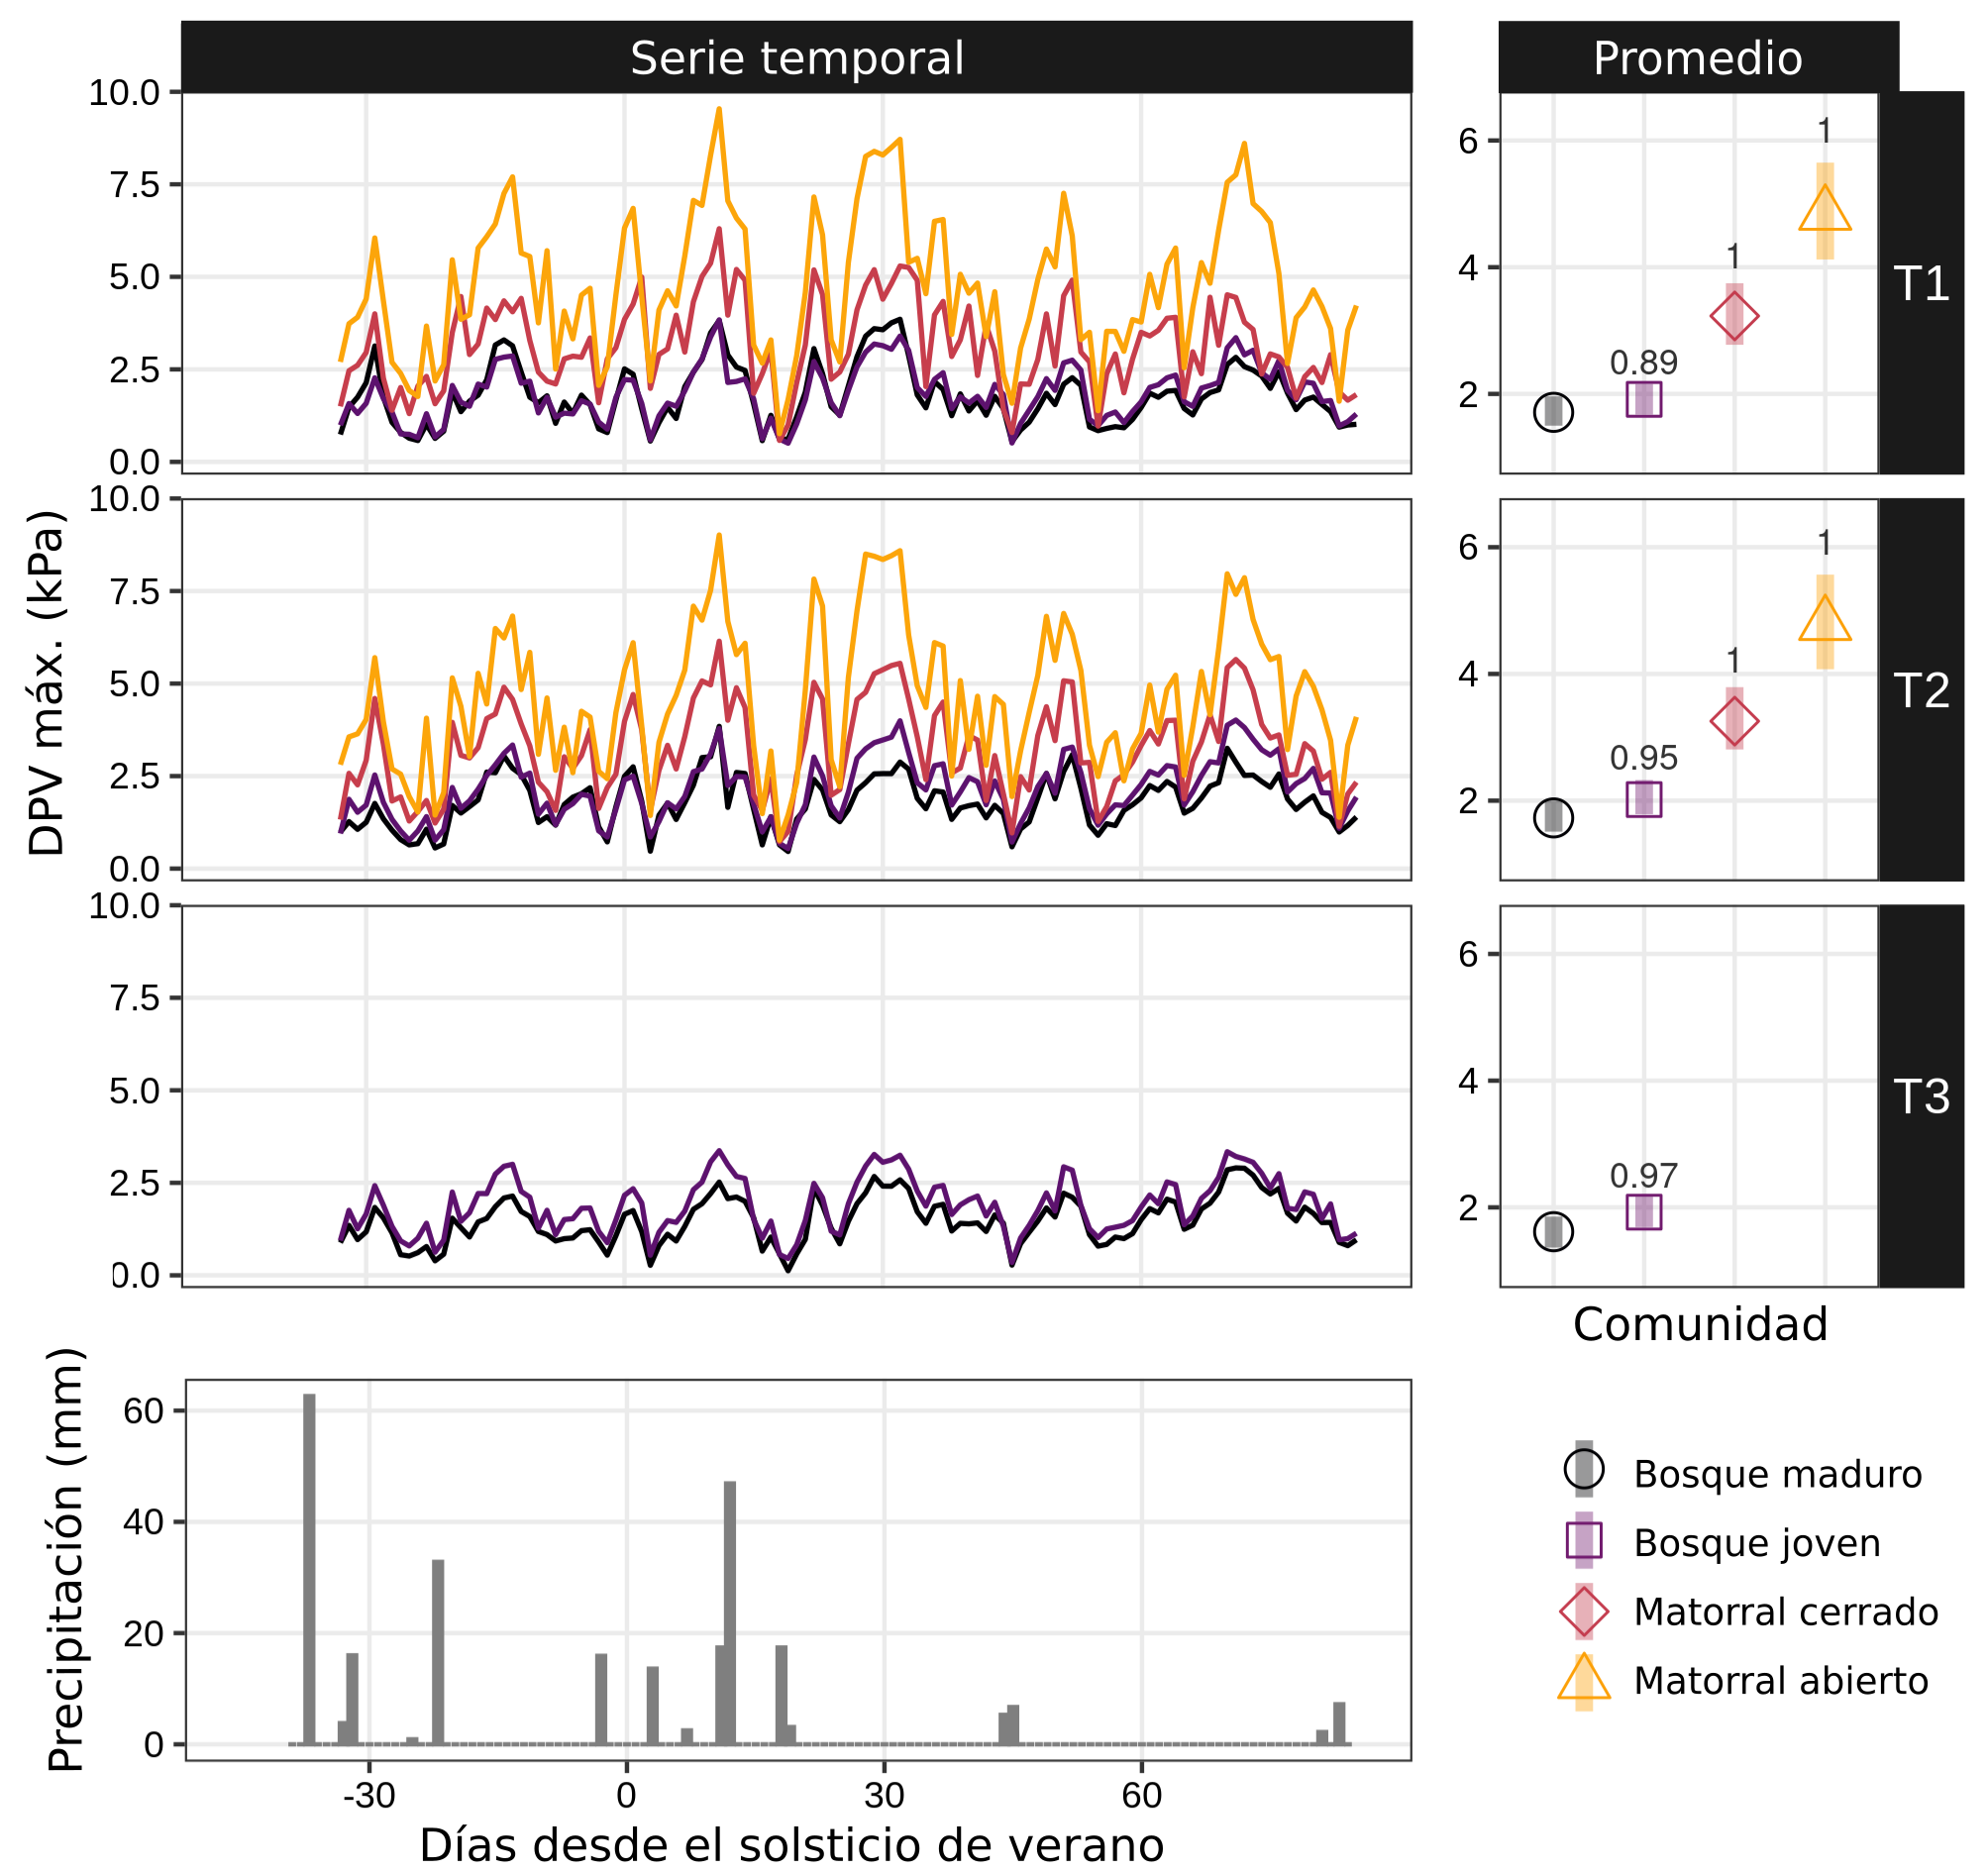
\includegraphics[width=16cm]{figuras/cap2/02) microclimate.png}
    \caption[Variación del microclima entre comunidades.]{Series temporales del Déficit de Presión de Vapor (DPV) máximo diario por comunidad y transecta (T), medido a $\approx$~50 cm sobre el suelo (paneles izquierdos). El día cero corresponde al 21 de diciembre de 2019. El panel inferior izquierdo muestra la precipitación diaria registrada en una estación meteorológica ubicada a 6 km del área de estudio. Los paneles derechos muestran el promedio estimado de DPV máximo por sitio (medias e intervalos de credibilidad del 95 \% de la distribución posterior), los cuales coinciden con los promedios observados. Los números sobre las barras indican la probabilidad posterior de que el promedio de DPV máximo en cada comunidad sea mayor que en el bosque maduro en su correspondiente transecta, estimada con el modelo de DPV. Los valores de probabilidad cercanos a 1 indican que una comunidad dada tiene un DPV mayor que el bosque maduro en su transecta (esperado), 0.5 indica que no hay diferencias, y valores cercanos a 0 indican un DPV mayor en el bosque maduro (no esperado).} 
    \label{fig:cap2-02}
\end{figure}

\subsection{Humedad del combustible}

\subsubsection{Combustibles muertos}

El contenido de humedad de la hojarasca (mezcla de combustibles) y el de las varillas de combustible (combustibles de composición similar) variaron entre comunidades de manera similar, pero de manera opuesta al DPV, siendo más bajo en los matorrales y mostrando una diferencia menor y más variable entre bosques jóvenes y maduros. Los matorrales abiertos presentaron un contenido de humedad ligeramente menor que los matorrales cerrados (Fig.~\ref{fig:cap2-03}a–\ref{fig:cap2-03}c). El contenido de humedad promedio por sitio mostró una relación negativa con el DPV máximo promedio del sitio (Fig.~\ref{fig:cap2-04}a–\ref{fig:cap2-04}c). El contenido de humedad de la hojarasca mostró mayor variabilidad que el de las varillas de combustible a todos los niveles (entre sitios, fechas y parcelas; Fig.~\ref{fig:cap2-03}a–\ref{fig:cap2-03}c y \ref{fig:cap2-S10}–\ref{fig:cap2-S12}).

\subsubsection{Combustibles vivos}

Los combustibles vivos de una sola especie (composición similar) mostraron un mayor contenido de humedad en los bosques maduros, con una relación negativa respecto al DPV, aunque esta relación no fue clara para todas las especies. En \textit{S. patagonicus}, este patrón fue consistente entre transectas, y el contenido de humedad mostró una clara relación negativa con el DPV (Fig.~\ref{fig:cap2-03}d y \ref{fig:cap2-04}d). En \textit{S. patagonicus}, al igual que en los combustibles muertos, los bosques jóvenes mostraron un contenido de humedad ligeramente menor que los bosques maduros, mientras que los matorrales presentaron valores mucho más bajos (Fig.~\ref{fig:cap2-03}d).

En \textit{N. dombeyi} y \textit{C. culeou}, las diferencias en el contenido de humedad entre comunidades fueron menores (Fig.~\ref{fig:cap2-03}e y \ref{fig:cap2-03}f). Para \textit{N. dombeyi}, el efecto del DPV fue despreciable, aunque con una tendencia negativa (Fig.~\ref{fig:cap2-04}e), y para \textit{C. culeou} encontramos un efecto negativo débil, pero su estimación fue bastante incierta debido al bajo número de sitios donde esta especie estuvo presente (Fig.~\ref{fig:cap2-04}f).

El contenido de humedad de la mezcla de combustibles vivos fue, en promedio, más alto en los matorrales, pero las diferencias entre comunidades variaron entre transectas: en la transecta 1, los matorrales abiertos y cerrados mostraron un mayor contenido de humedad que el bosque maduro, mientras que en la transecta 2 estas comunidades mostraron valores similares. Los bosques jóvenes tuvieron un menor contenido de humedad que los bosques maduros en las transectas 1 y 2, pero se observó lo contrario en la transecta 3 (Fig.~\ref{fig:cap2-03}g). En la transecta 1, los valores más altos de contenido de humedad se observaron al inicio del verano, y las comunidades mostraron valores más similares hacia el final (Fig. \ref{fig:cap2-S16}).

El contenido de humedad de la mezcla de combustibles vivos mostró una relación positiva con el DPV (Fig.~\ref{fig:cap2-04}g). El ordenamiento de los sitios con respecto a la composición de especies que conforman el combustibles vivo mostró que el eje principal de variación (eje 1, Fig.~\ref{fig:cap2-05}) estaba correlacionado con el contenido de humedad promedio (coeficiente de correlación de Pearson = -0.81), lo que indica que el contenido de humedad está asociado a la composición de especies.

\begin{figure}[htbp]
    \centering
    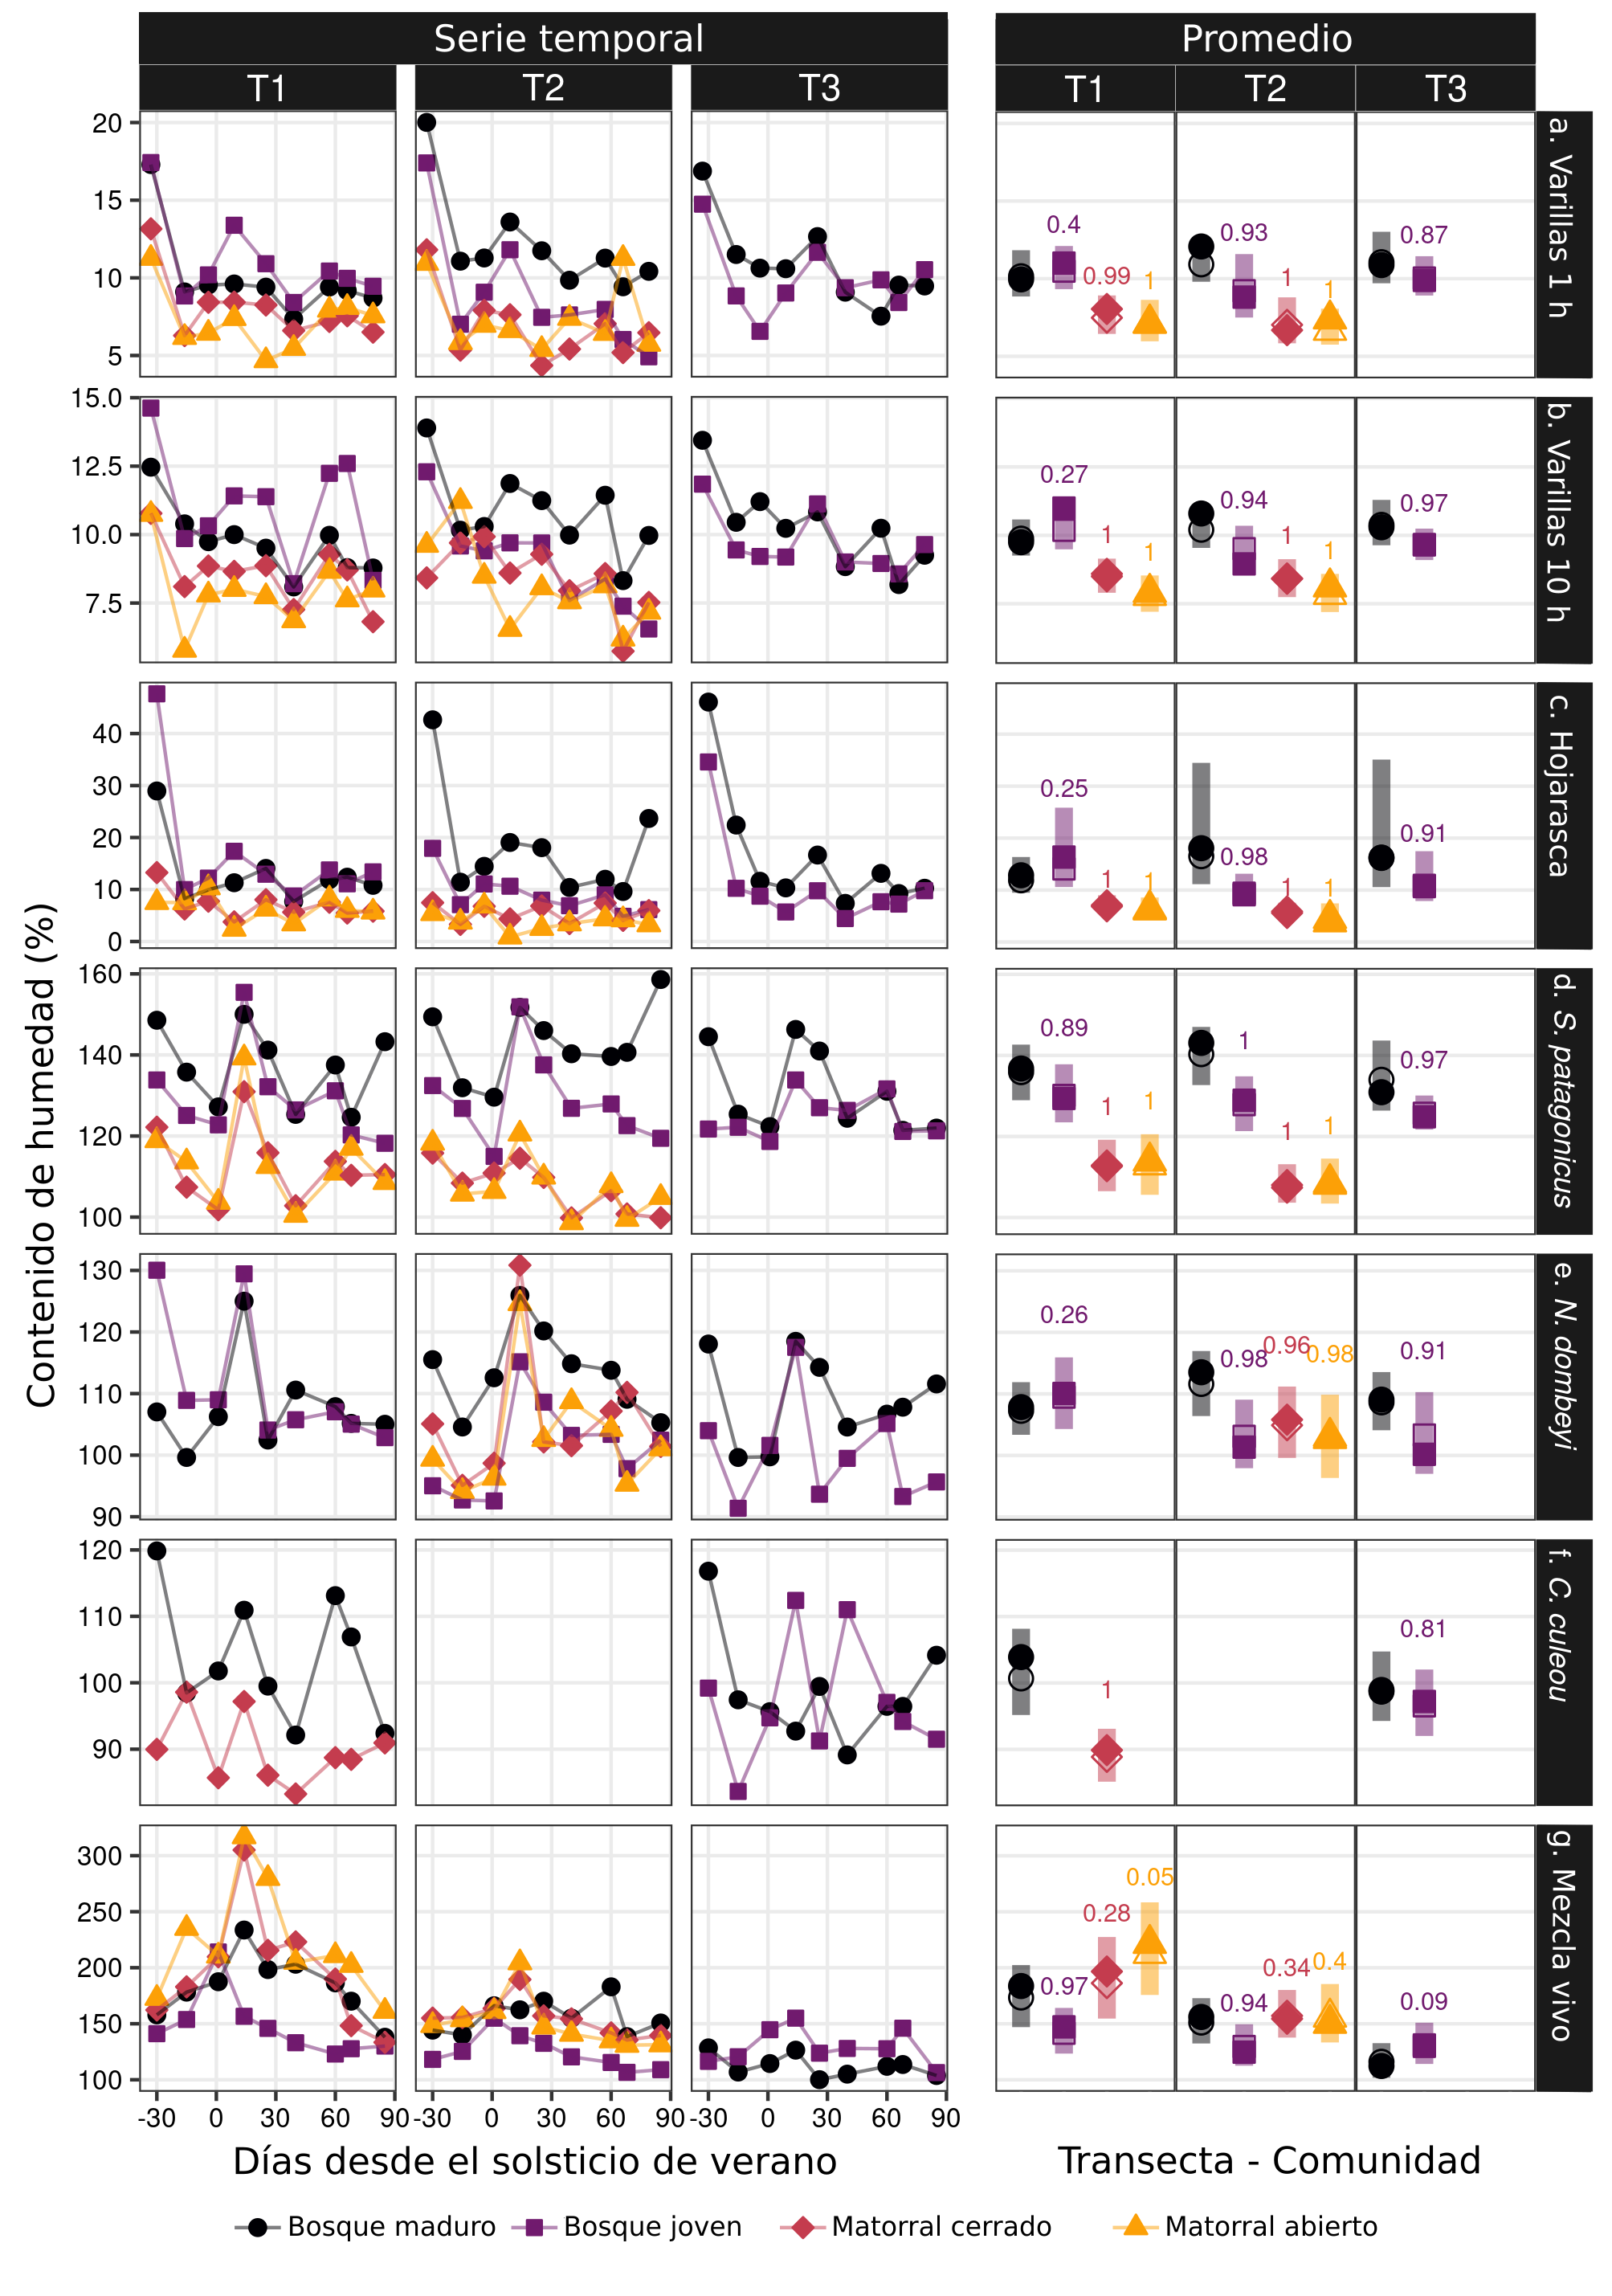
\includegraphics[width=15cm]{figuras/cap2/03) moisture ts.png}
    \caption[Variación del contenido de humedad del combustible entre comunidades.]{(Leyenda en la página siguiente.)}
    \label{fig:cap2-03}
\end{figure}

% leyenda en la página siguiente
\begin{figure}[p]
  \contcaption{(en la página anterior). Contenido de humedad del combustible por tipo de combustible, comunidad y transecta. Los valores para todas las fechas de muestreo se muestran en los paneles izquierdos, y los promedios de la temporada se presentan en los paneles derechos. El día cero corresponde al 21 de diciembre de 2019. En los paneles derechos, los símbolos abiertos y las barras muestran la media y el intervalo de credibilidad del 95 \% de la distribución posterior para el contenido de humedad promedio en cada sitio, estimados por los GLMMs, mientras que los símbolos llenos muestran las medias observadas. Los números sobre las barras indican la probabilidad posterior de que el contenido de humedad promedio en cada comunidad sea menor que en el bosque maduro de su correspondiente transecta. Los valores cercanos a 1 indican que una comunidad dada tiene un menor contenido de humedad que el bosque maduro en su transecta (esperado), 0.5 indica que no hay diferencias, y valores cercanos a 0 indican un menor contenido de humedad en el bosque maduro (no esperado).}
\end{figure}

\begin{figure}[htbp]
    \centering
    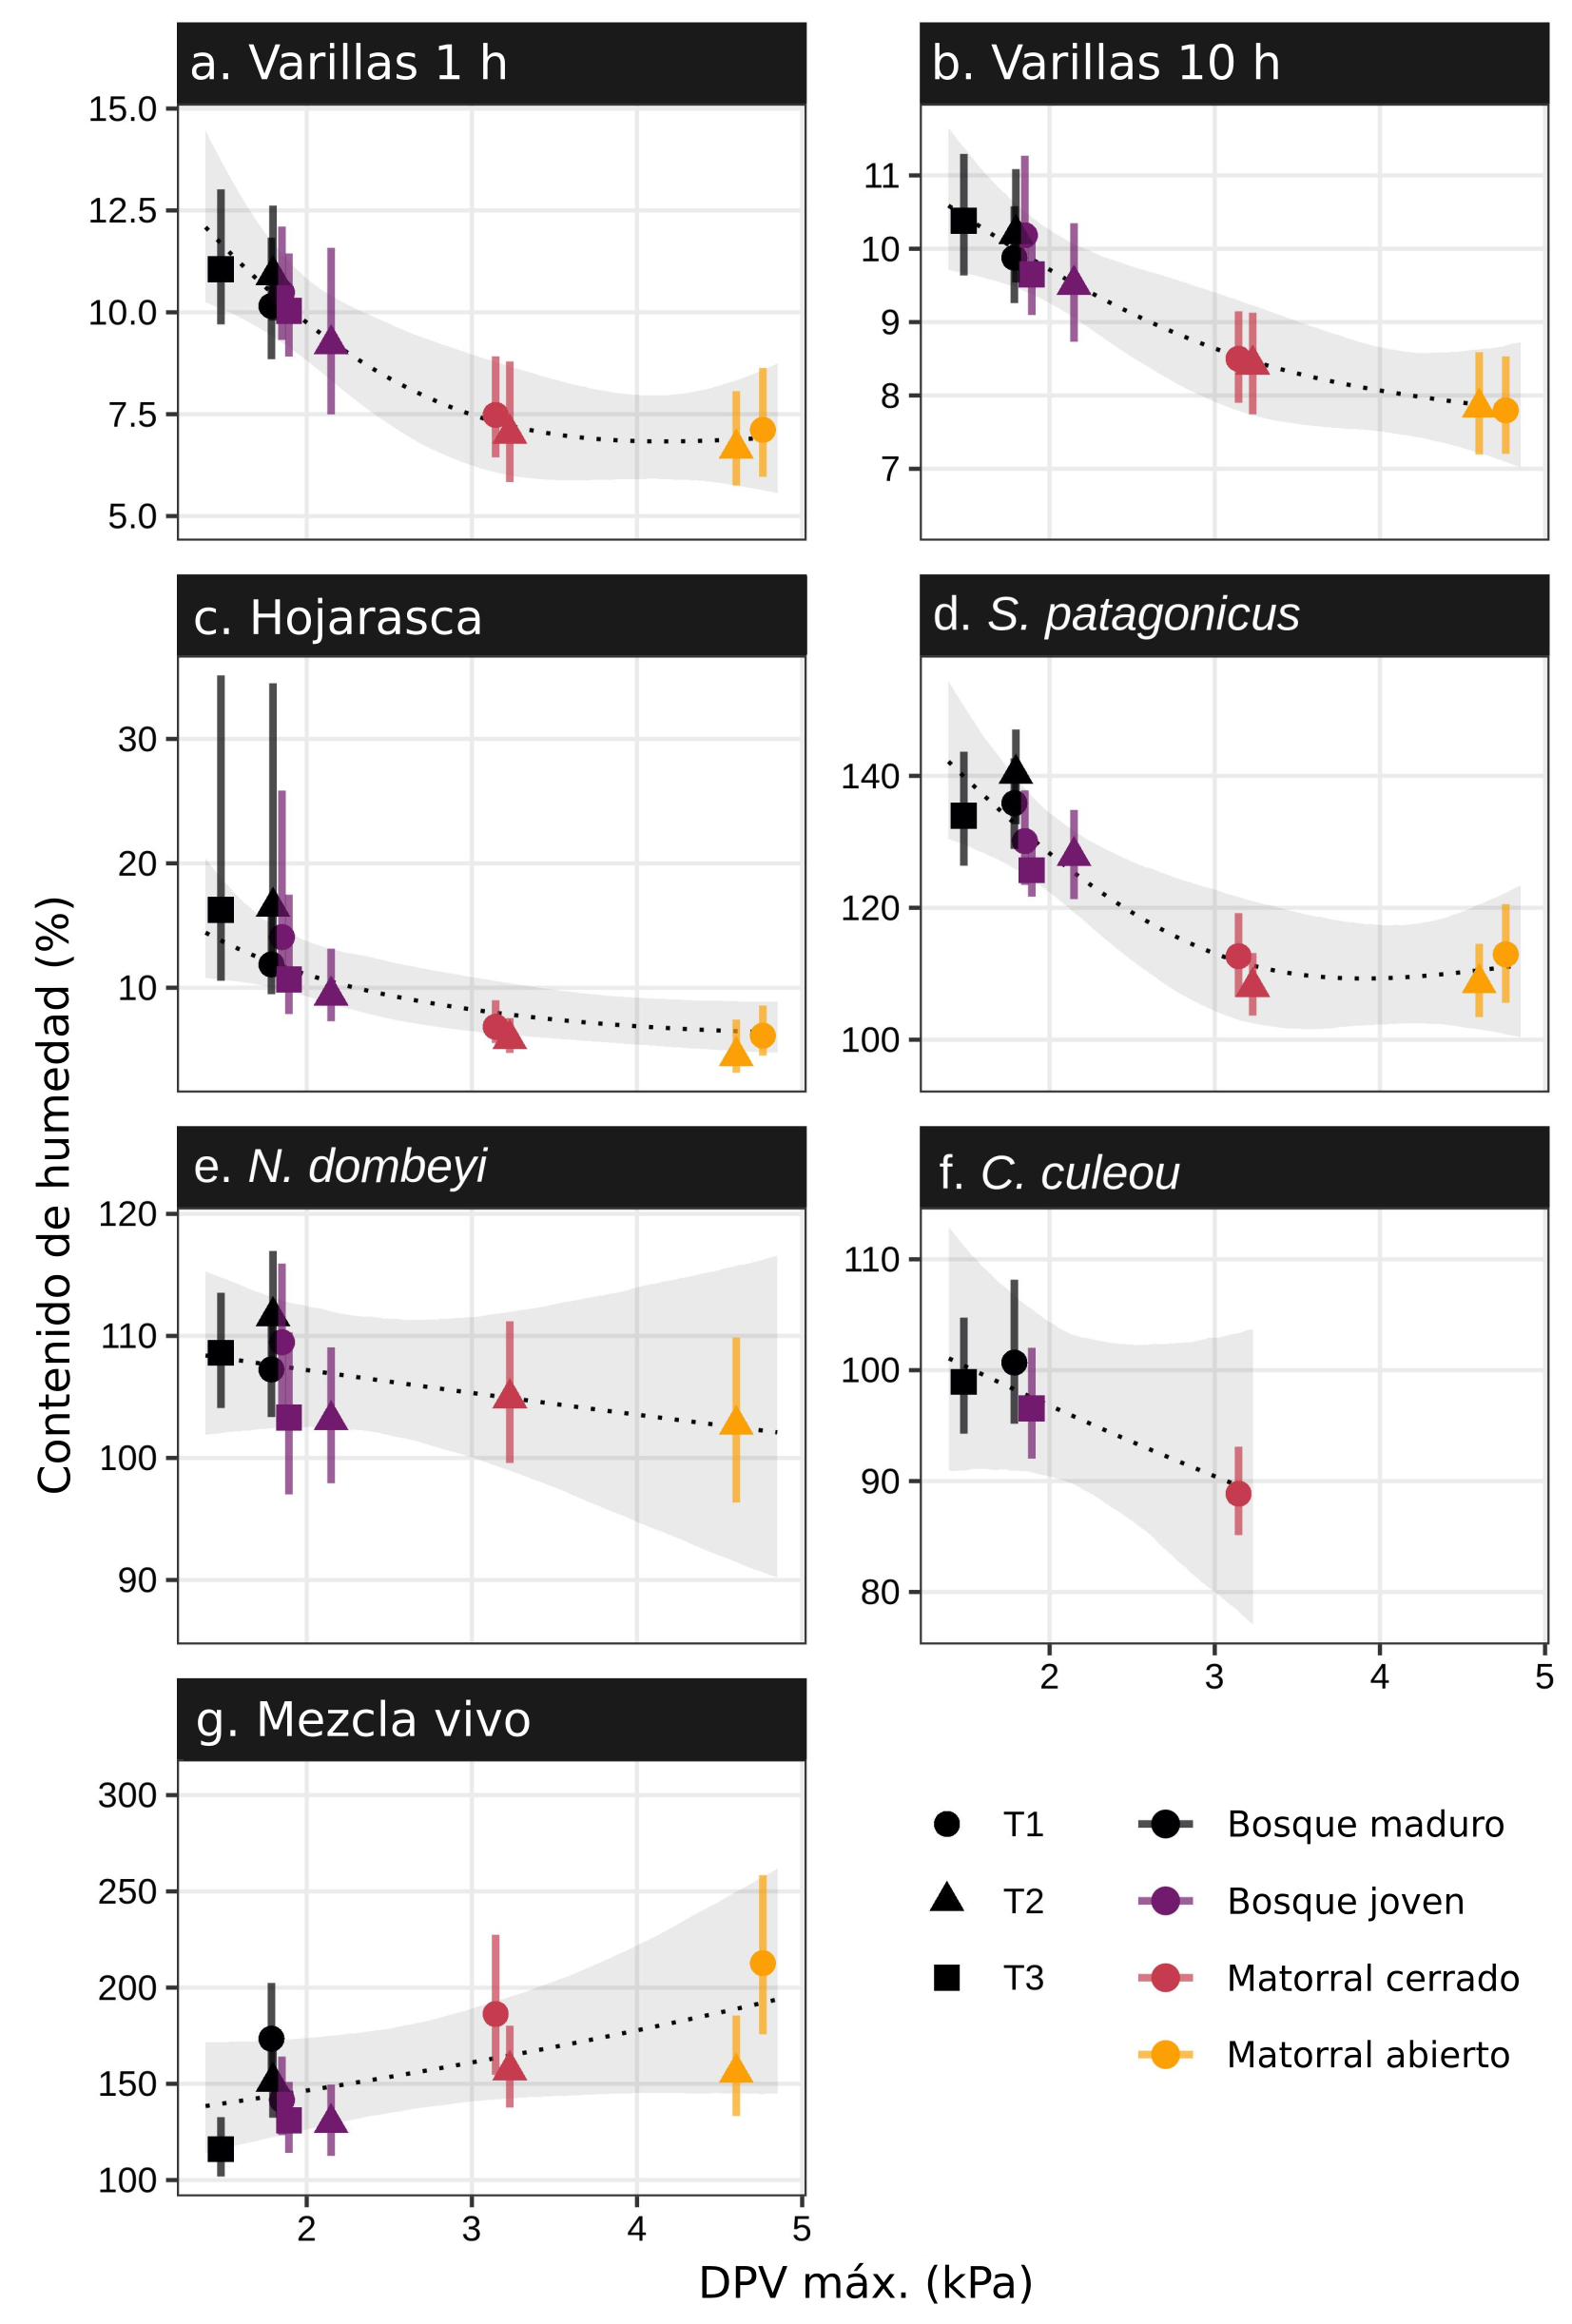
\includegraphics[width=13cm]{figuras/cap2/04) humedad - vpd.png}
    \caption[Contenido de humedad del combustible en función del Déficit de Presión de Vapor.]{Contenido de humedad promedio estimado en función del DPV máximo promedio por sitio. Los puntos representan la media de la distribución posterior para cada sitio, y las barras, los intervalos de credibilidad del 95 \% (mismos valores que en el panel derecho de la Fig.\ref{fig:cap2-03}). El efecto estimado del DPV se muestra con la línea punteada (media de la posterior) y la banda gris (IC del 95 \%).} 
    \label{fig:cap2-04}
\end{figure}

\begin{figure}[htbp]
    \centering
    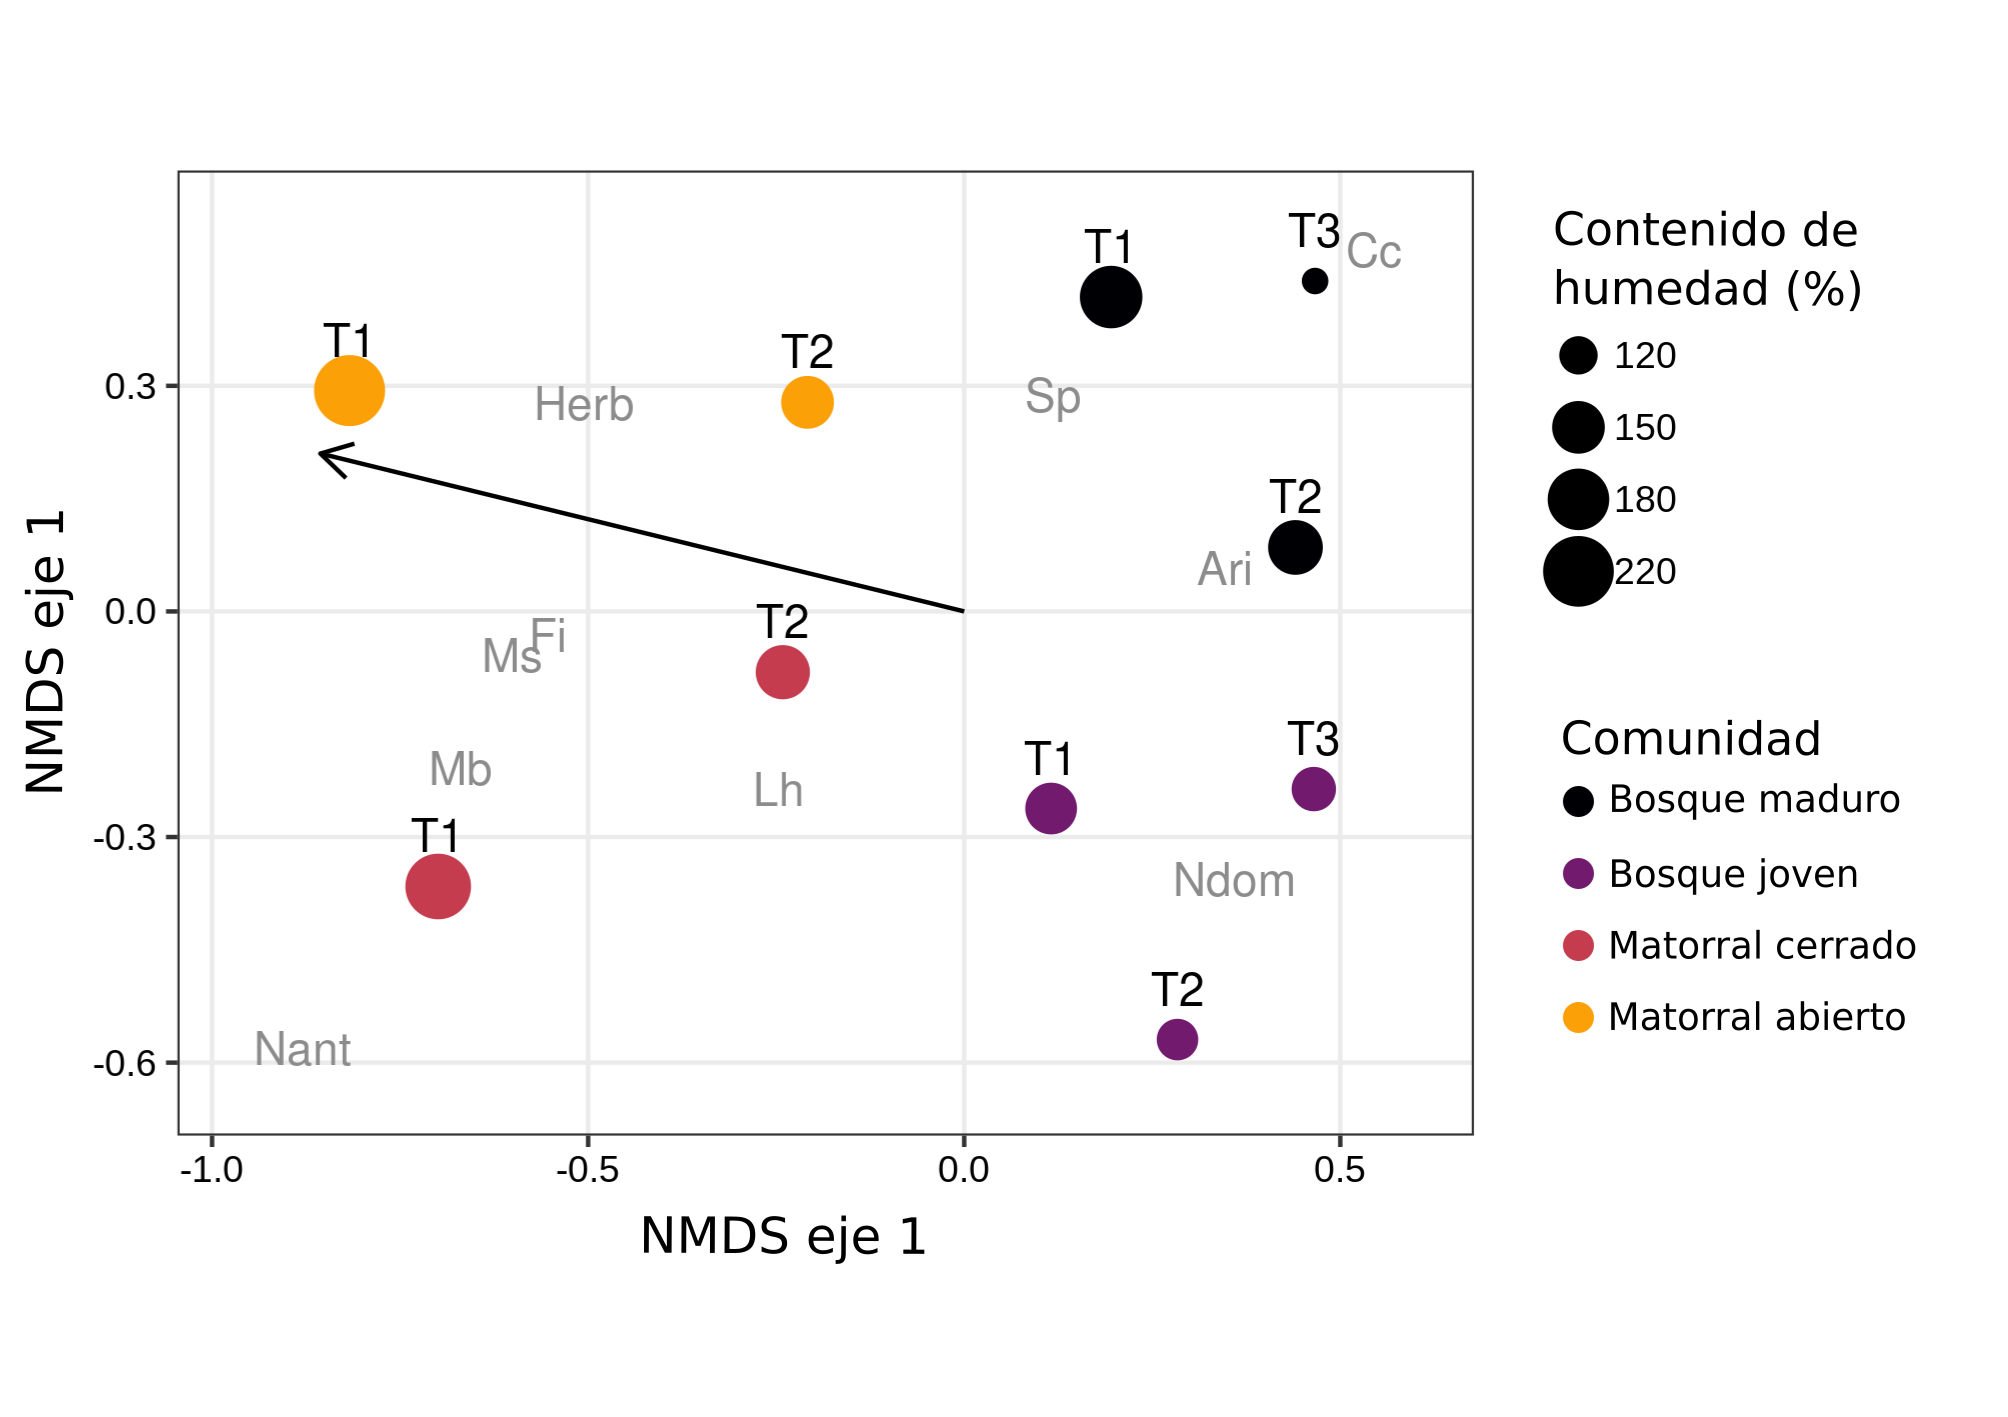
\includegraphics[width=15cm]{figuras/cap2/05) ordination.png}
    \caption[Ordenamiento de sitios según la composición de especies.]{Ordenamiento de sitios según la composición y abundancia de especies. Escalamiento Multidimensional No Métrico (NMDS) calculado a partir de los datos de intersección con varilla considerando solo combustibles vivos (\textit{stress} = 0.079; $\text{R}^2 \ \text{lineal} = 0.958$). Los sitios más cercanos en el gráfico son aquellos con una mayor similitud en la abundancia relativa de especies. Las coordenadas de la punta de la flecha muestran el coeficiente de correlación de Pearson entre los ejes y el contenido de humedad promedio de la mezcla de combustibles vivos por sitio (representado por el tamaño de los puntos). El texto en negro identifica las transectas, y el texto en gris, las coordenadas de las 10 especies más abundantes (Ndom: \textit{Nothofagus dombeyi}, Herb: especies herbáceas, Sp: \textit{Schinus patagonicus}, Cc: \textit{Chusquea culeou}, Ms: \textit{Mutisia spinosa}, Lh: \textit{Lomatia hirsuta}, Fi: \textit{Fabiana imbricata}, Ari: \textit{Aristotelia chilensis}, Nant: \textit{Nothofagus antarctica}, Mb: \textit{Maytenus boaria}).} 
    \label{fig:cap2-05}
\end{figure}

\FloatBarrier

\subsection{Probabilidad de ignición y disponibilidad del combustible}

Las diferencias en el contenido de humedad del combustible entre comunidades tuvieron un efecto claro en la probabilidad de ignición media, tanto para la hojarasca como para la mezcla de combustibles vivos. Para la hojarasca, la probabilidad de ignición en los bosques maduros estuvo mayormente por debajo de 0.9, mientras que en las demás comunidades tendió a ser más alta. En particular, los matorrales mostraron probabilidades de ignición superiores a 0.97 (Fig.~\ref{fig:cap2-06}, paneles superiores).

La probabilidad de ignición de la mezcla de combustibles vivos mostró un patrón variable entre transectas, al igual que su contenido de humedad. Los bosques jóvenes presentaron la mayor probabilidad de ignición, excepto en la transecta 3, donde fue mayor en el bosque maduro. Los matorrales mostraron una probabilidad de ignición menor que el bosque maduro en la transecta 1, y valores similares en la transecta 2 (Fig.~\ref{fig:cap2-06}, paneles inferiores).

La disponibilidad de combustible para la hojarasca mostró grandes diferencias entre comunidades, especialmente cuando se consideró el umbral de humedad para peligro de incendios extremo ($\le 9.85$ \%). En los bosques maduros, la humedad de la hojarasca cayó por debajo del umbral de 9.85 \% en solo 1 o 2 fechas de 9. En cambio, el contenido de humedad de los matorrales (abiertos o cerrados) estuvo por debajo de este umbral en la mitad o más de las fechas (Tabla~\ref{tab:fuel-availability}). Los bosques jóvenes mostraron una situación intermedia, cayendo por debajo del umbral crítico con mayor frecuencia que los bosques maduros, pero menor que los matorrales.

Todas las comunidades mostraron un contenido de humedad promedio de la hojarasca por debajo del umbral superior ($< 23.75$ \%) durante casi todas las fechas (8 o 9 de 9). Solo el 11 \% de las fechas mostraron simultáneamente humedad de la hojarasca en los matorrales $\le 9.85$ \%
y en los bosques maduros $> 23.75$ \% (Tabla~\ref{tab:fuel-availability}). Finalmente, el contenido de humedad promedio de la mezcla de combustibles vivos muy raramente cayó por debajo del 110 \%, con una tendencia a que esta condición ocurriera con mayor frecuencia en bosques maduros y jóvenes que en matorrales (Tabla~\ref{tab:fuel-availability}).

\begin{figure}[htbp]
    \centering
    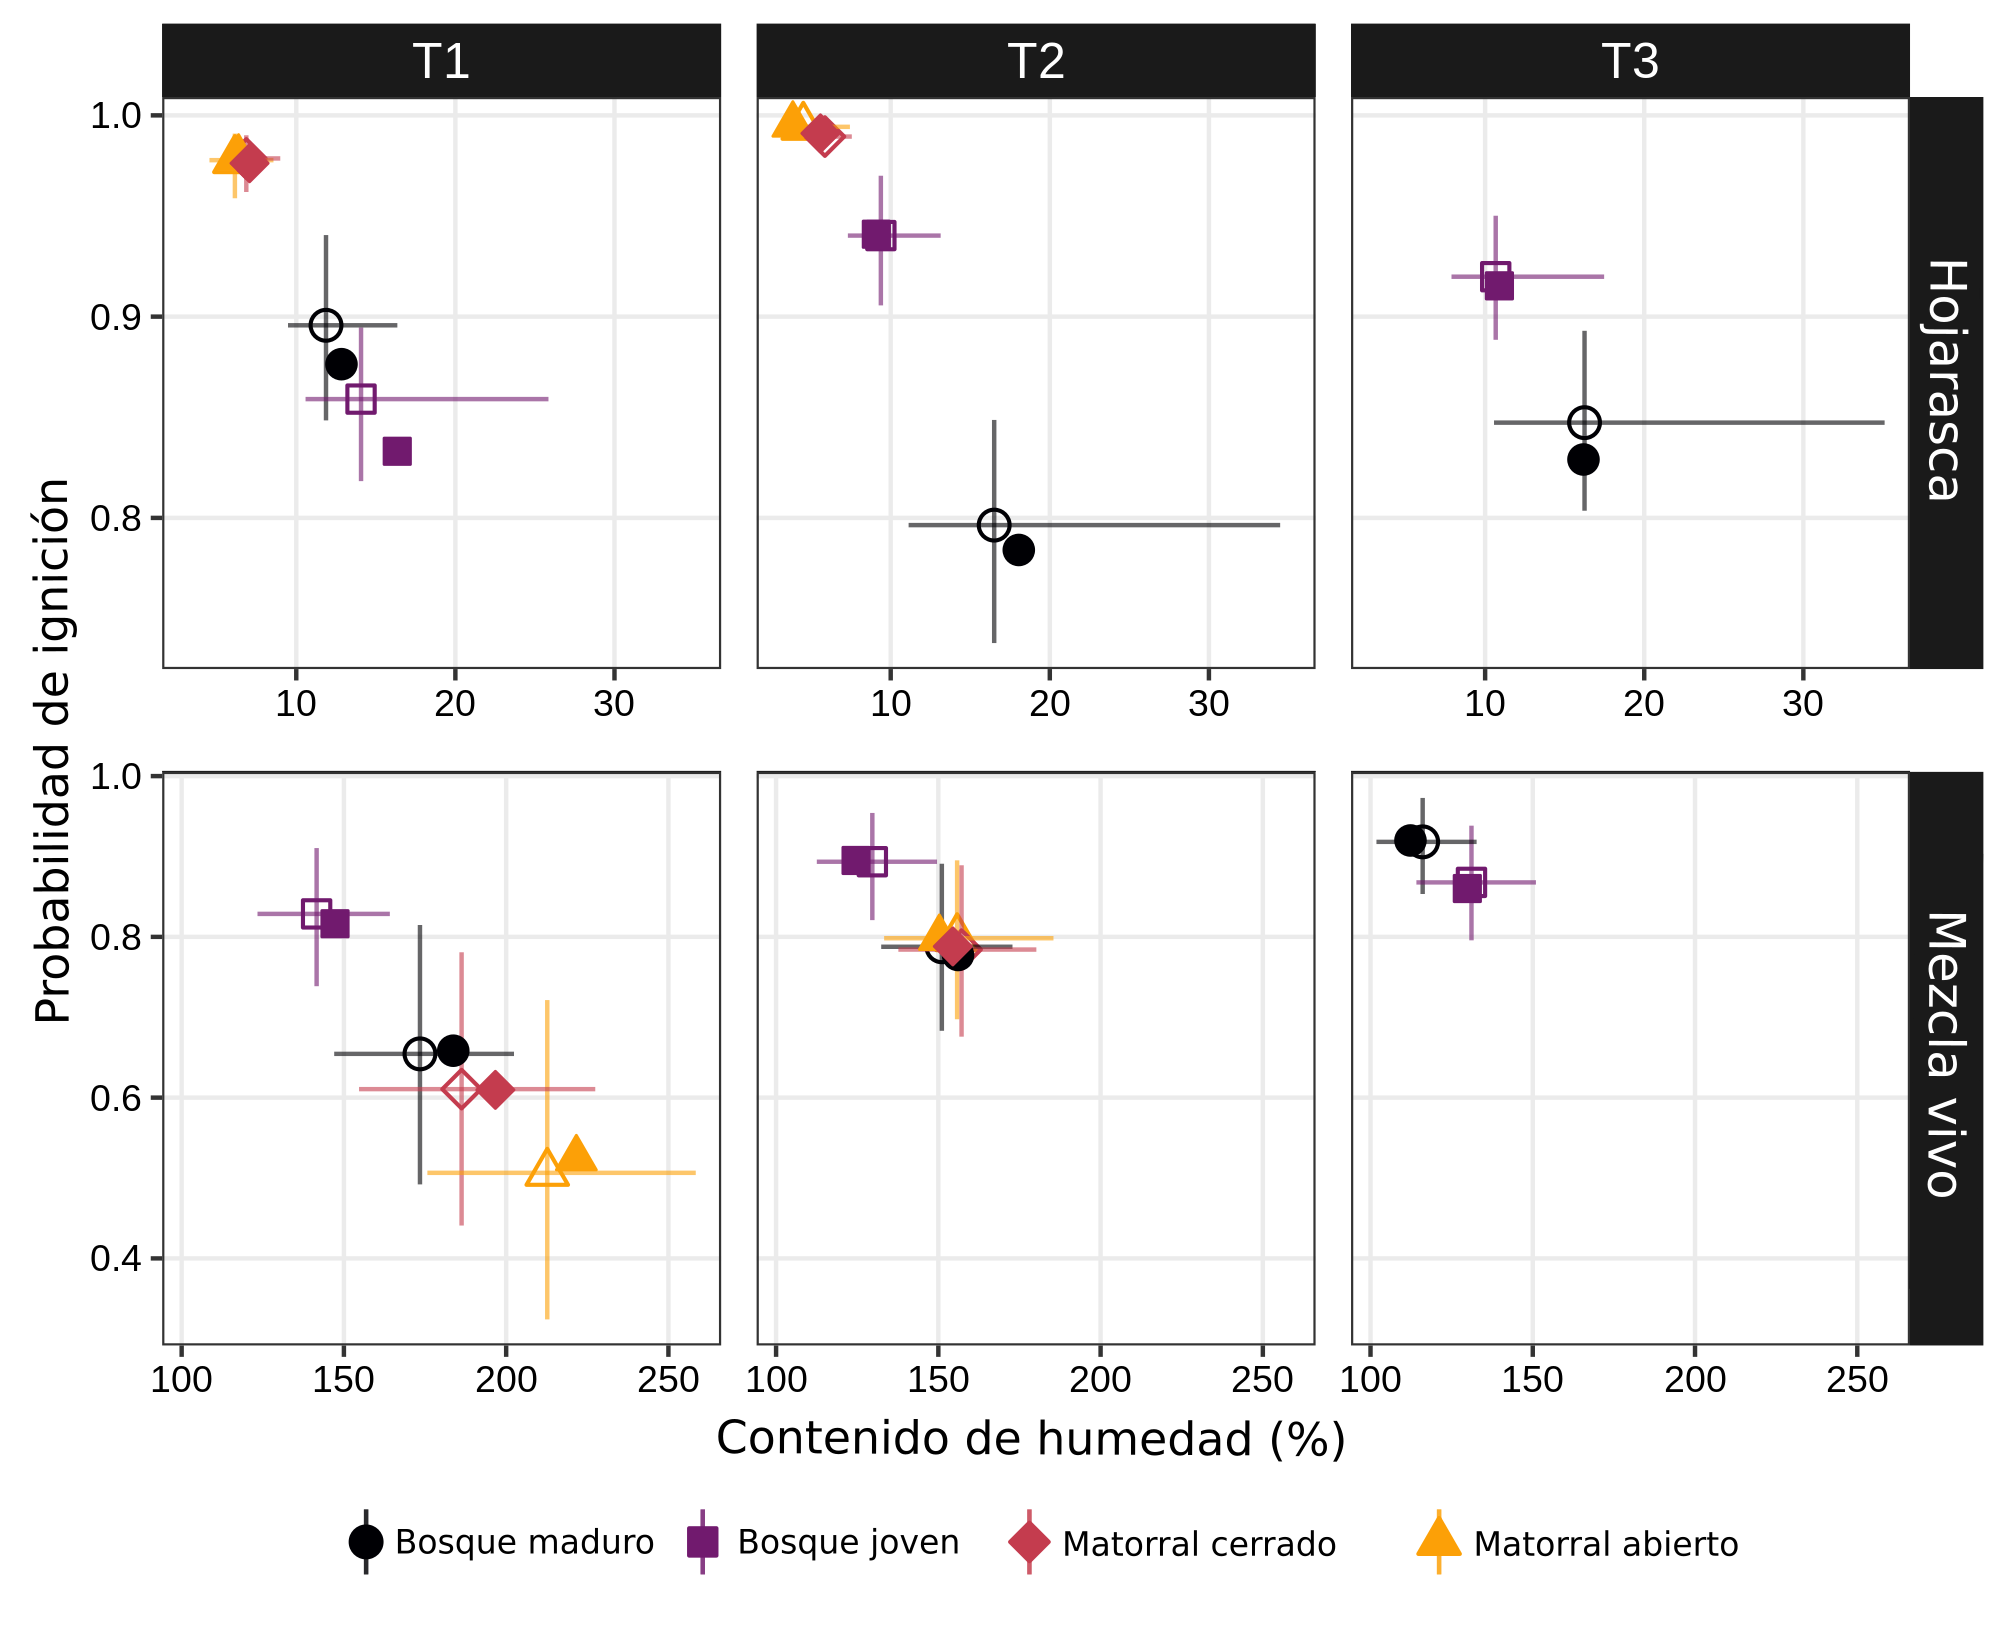
\includegraphics[width=16cm]{figuras/cap2/06) ig probability.png}
    \caption[Probabilidad de ignición.]{Probabilidad de ignición en función del contenido de humedad por comunidad, transecta y tipo de combustible. Los símbolos sólidos muestran la probabilidad de ignición y los promedios de contenido de humedad del combustible basados en los datos observados. Los símbolos abiertos y las barras muestran la media de la distribución posterior y los intervalos de mayor densidad del 95 \% basados en los valores de contenido de humedad del combustible simulados con los GLMMs.} 
    \label{fig:cap2-06}
\end{figure}

\begin{table}[ht]
\centering
\caption[Comparación de la disponibilidad de combustibles entre comunidades]{Comparación de la disponibilidad de combustibles entre comunidades. La disponibilidad de combustibles es el porcentaje de fechas (n = 9) en las que el contenido de humedad (CH) promedio estuvo por debajo de los umbrales críticos de peligro de incendios. Los umbrales de contenido de humedad de la hojarasca, 23.75 \% y 9.85 \%, son valores por debajo de los cuales la probabilidad de ignición de la hojarasca excede 0.5 y 0.98, respectivamente, según pruebas de ignición en laboratorio de \citet{bianchi_ignition_2014}. El umbral del 110 \% para la mezcla de combustibles vivos representa el contenido de humedad por debajo del cual se ha reportado la ocurrencia de incendios de gran magnitud en este sistema y otros similares \citep{chuvieco_prediction_2009, bianchi_live_2015, arganaraz_determining_2018}.}
\label{tab:fuel-availability}
\resizebox{16cm}{!}{%
\begin{tabular}{llccccc}
\toprule
\makecell{Tipo de\\combustible} & \makecell[c]{Umbral / comparación} & Transecta & \makecell{Bosque\\maduro} & \makecell{Bosque\\joven} & \makecell{Matorral\\cerrado} & \makecell{Matorral\\abierto} \\
\midrule
\multirow{9}{*}{Hojarasca} & \multirow{3}{*}{CH $\le$ 23.75 \%} & T1 & 88.89 & 88.89 & 100 & 100 \\
                        &  & T2 & 88.89 & 100 & 100 & 100 \\
                        &  & T3 & 88.89 & 88.89 & - & - \\
                        \cline{2-7}
                        & \multirow{3}{*}{CH $\le$ 9.85 \%} & T1 & 22.22 & 11.11 & 88.89 & 88.89 \\
                        & & T2 & 11.11 & 66.67 & 100 & 100 \\
                        & & T3 & 22.22 & 77.78 & - & - \\
                        \cline{2-7}
                        & \multirow{3}{*}{\makecell[l]{CH $>$ 23.75 \% en bosque maduro\\y $\le$ 9.85 \% en las demás}} & T1 & - & 0 & 0 & 11.11 \\
                        & & T2 & - & 0 & 11.11 & 11.11 \\
                        & & T3 & - & 0 & - & - \\
                        \cline{2-7}
\multirow{3}{*}{\makecell[l]{Mezcla de\\combustible vivo}} & \multirow{3}{*}{CH $\le$ 110 \%} & T1 & 0 & 0 & 0 & 0 \\
                                   & & T2 & 0 & 22.22 & 0 & 0 \\
                                   & & T3 & 44.44 & 11.11 & - & - \\
\bottomrule
\end{tabular}%
}
\end{table}

\FloatBarrier

\section{Discusión}

\subsection{Microclima}

Como se esperaba, encontramos un DPV máximo y una temperatura del aire más altos, junto con una humedad relativa mínima más baja en los sitios más abiertos en comparación con los bosques maduros. Esto concuerda con un estudio previo en bosques subalpinos de \textit{N. pumilio} \citep{paritsis_positive_2015} y con otros estudios en bosques templados y tropicales \citep{uhl_fire_1988, little_fire_2012, hoffmann_fuels_2012, jucker_canopy_2018, de_frenne_global_2019, kane_stand_2021, wolf_wildfire_2021}. Por el contrario, \citet{burton_shifting_2019} reportaron variaciones muy pequeñas en estas variables entre estados alternativos en bosques templados del sureste de Australia. Una posible razón para esta discrepancia podría ser que sus comunidades quemadas más recientemente tenían vegetación alta (10-15 m) y densa, probablemente albergando un microclima relativamente más fresco y húmedo que nuestros matorrales (con 1 a 4 m de altura).

Encontramos que los bosques jóvenes mostraron extremos de DPV, temperatura y humedad relativa similares a los bosques maduros. Esto podría explicarse por su alta densidad de vegetación desde el suelo hasta los 4 m de altura, que fue mucho menor en los matorrales cerrados y abiertos (Fig.~\ref{fig:cap2-S02} y \ref{fig:cap2-S03}). Sin embargo, las diferencias microclimáticas entre comunidades podrían variar si se consideran otras alturas \citep{pickering_darker_2021}. Por ejemplo, los bosques jóvenes, al carecer de un dosel alto, presentan menor cobertura de vegetación que los bosques maduros por encima de 1.5 m de altura (en lugar de 0.5 m, donde se instalaron los sensores; Fig.~\ref{fig:cap2-S04}). Por lo tanto, el DPV a 1.5 m probablemente sería más alto en los bosques jóvenes que en los maduros.

\subsection{Variación del contenido de humedad entre comunidades y su relación con el DPV}

Como esperábamos, el contenido de humedad de los combustibles muertos mostró una relación negativa con el DPV, probablemente reflejando el efecto del microclima sobre la tasa de evaporación, en concordancia con estudios previos \citep{uhl_fire_1988, hoffmann_fuels_2012, little_fire_2012, balch_susceptibility_2015, kane_stand_2021}. Nuestros resultados son consistentes con \citet{brown_sensitivity_2022}, quienes encontraron que el DPV en el sotobosque fue una de las variables microclimáticas más importantes controlando el contenido de humedad de varillas de combustible de 10 h en bosques templados del sureste de Australia. Sin embargo, dado que la estructura de la vegetación controla también otras variables microclimáticas, es probable que los sitios más abiertos (e.g., matorrales) no solo muestren un DPV más alto, sino también mayor radiación solar y mayor velocidad del viento \citep{little_fire_2012, jucker_canopy_2018, de_frenne_global_2019, wolf_wildfire_2021}. Por lo tanto, el efecto del DPV que observamos sobre el contenido de humedad de combustibles muertos probablemente refleja un efecto compuesto de todas estas variables microclimáticas correlacionadas.

La estructura de la vegetación también podría explicar las similitudes observadas en el DPV y, consecuentemente, en el contenido de humedad de combustibles muertos entre bosques jóvenes y maduros. Este resultado concuerda parcialmente con \citet{brown_forest_2021}, quienes encontraron una relación positiva entre el contenido de humedad de las varillas de combustible de 10 h y la densidad de la vegetación entre 0.5 y 2 m de altura en bosques templados del sureste de Australia. Tanto las mezclas como los combustibles muertos de composición similar (hojarasca y varillas de combustible) mostraron la misma relación entre el contenido de humedad y el DPV, lo que sugiere que la composición de especies no ejerce un control importante sobre el contenido de humedad de la hojarasca. Sin embargo, la mayor variabilidad en el contenido de humedad de la hojarasca entre sitios, fechas y parcelas, en comparación con las varillas de combustible, podría explicarse parcialmente por la composición de la hojarasca.

En cuanto a los combustibles vivos, encontramos que un microclima más húmedo y fresco promueve un mayor contenido de humedad dentro de una misma especie, pero el patrón opuesto se observó a nivel comunitario. Los combustibles vivos de una sola especie tendieron a mostrar mayor contenido de humedad en los sitios más frescos y húmedos, particularmente en el arbusto \textit{S. patagonicus}. Los efectos microclimáticos estimados mostraron una considerable incertidumbre en el caso de \textit{C. culeou} y \textit{N. dombeyi}, probablemente debido al reducido número de sitios (cuatro y seis, comparado con los 10 de \textit{S. patagonicus}), aunque este patrón coincide con los resultados de \citet{blackhall_is_2012} para un mayor número de sitios y especies. Las autoras reportaron que las plantas en comunidades posfuego usualmente tienen rasgos foliares más inflamables (incluyendo menor contenido de humedad) en comparación con las mismas especies en sitios no quemados. Como se mencionó para los combustibles muertos, el efecto del DPV sobre el contenido de humedad de combustibles vivos de una sola especie probablemente refleja un efecto compuesto de otras variables microclimáticas correlacionadas, como la radiación y la velocidad del viento, que actuarían durante la etapa de desarrollo del tejido foliar \citep{aroca_plant_2012}.

El contenido de humedad a nivel comunitario (mezclas de combustibles vivos) mostró un patrón opuesto al de los combustibles vivos de una sola especie, siendo mayor o similar en los sitios más desecantes. Esto sugiere que el microclima afecta los rasgos de las plantas dentro de una especie, pero no necesariamente promueve la dominancia de especies esclerófilas en los sitios más desecantes. La relación positiva entre el DPV y el contenido de humedad de las mezclas de combustibles vivos está influenciada por los altos valores encontrados en los matorrales de la transecta 1, mientras que los matorrales de la transecta 2 mostraron valores similares a los de las otras comunidades. Estas variaciones podrían explicarse parcialmente por la composición y abundancia de especies. Por ejemplo, el bajo contenido de humedad en los bosques maduros y jóvenes probablemente esté relacionado con su alta abundancia de \textit{N. dombeyi} y \textit{C. culeou} (Tabla~\ref{tab:sp-composition} y Fig.~\ref{fig:cap2-S05}), especies cuyo contenido de humedad medio es bajo y muy bajo, respectivamente \citep{bianchi_comparison_2018, blackhall_flammability_2019}. Además, el bajo contenido de humedad en el bosque maduro de la transecta 3 podría explicarse por su alta abundancia relativa de \textit{C. culeou} ($\approx$~60 \%, Tabla~\ref{tab:sp-composition} y Fig.~\ref{fig:cap2-S05}). Por otro lado, la presencia de pastos y otras plantas herbáceas (como \textit{Vicia} sp., observada en los matorrales estudiados) podría aumentar el contenido de humedad en los matorrales.

También encontramos que en la transecta 1 la variabilidad en el contenido de humedad entre comunidades fue grande a mediados del verano, pero pequeña al inicio y final de la estación seca (Fig.~\ref{fig:cap2-S16}). Estas dinámicas estacionales suelen resultar de cambios no solo en el contenido de agua, sino también en el contenido de materia seca \citep{jolly_-coupling_2014, qi_spectroscopic_2014}. Algunas especies, como \textit{N. dombeyi}, \textit{N. antarctica}, o plantas herbáceas, producen follaje nuevo hacia fines de la primavera, aumentando su contenido de humedad, mientras que otras alcanzan su contenido máximo de humedad a principios o finales del verano, probablemente cuando producen nuevas hojas (e.g., \textit{Lomatia hirsuta}, \textit{Austrocedrus chilensis} y \textit{Maytenus boaria}; Kitzberger, datos no publicados). Los cambios en la humedad del suelo relacionados con la lluvia también podrían haber contribuido a estas variaciones temporales en el contenido de humedad de las mezclas de combustibles vivos, pero el hecho de que solo en la transecta 1 se haya observado un pico en el contenido de humedad vuelve esta explicación poco plausible.

\subsection{Contribución de la humedad del combustible a las diferencias de inflamabilidad}

Nuestros resultados sugieren que el contenido de humedad de la hojarasca contribuye a la diferencia de inflamabilidad entre comunidades pirófilas y pirófobas. El menor contenido de humedad en la hojarasca de los matorrales en comparación con los bosques maduros resultó en una mayor probabilidad de ignición y disponibilidad de combustible en los primeros. Al comparar bosques maduros y jóvenes, la diferencia en la probabilidad de ignición y disponibilidad de combustible fue menor, lo que sugiere que el contenido de humedad de la hojarasca presenta una contribución pequeña a su diferencia en inflamabilidad.

La contribución del contenido de humedad de la hojarasca a las diferencias de inflamabilidad entre comunidades depende de cómo la estructura de la vegetación sobre la hojarasca controla el microclima cercano a la superficie. Aunque los bosques jóvenes carecen de un dosel alto, su alta densidad de árboles y arbustos jóvenes, de alrededor de 4 m de altura, genera un microclima sombreado cerca de la superficie. Nuestros resultados se asemejan a patrones descritos en bosques templados de eucaliptos (sureste de Australia), donde la edad del rodal y la estructura del dosel por sí solas no explican las variaciones en el contenido de humedad de la hojarasca \citep{cawson_fuel_2017, burton_shifting_2019, brown_forest_2021}. Por ejemplo, \citet{cawson_fuel_2017} reportaron mayor contenido de humedad en combustibles muertos en comunidades con regeneración vigorosa tras un incendio severo en comparación con bosques antiguos más abiertos o bosques tras incendios de baja severidad, donde la regeneración era escasa. Contrariamente, \citet{burton_shifting_2019} encontraron que los bosques no quemados por largos períodos albergan un elevado contenido de humedad en combustibles muertos, asociado a una densa capa de helechos cerca de la superficie. En nuestro estudio, los matorrales jóvenes cerrados, eran, aparentemente, lo suficientemente abiertos como para que la hojarasca mostrara un menor contenido de humedad que en los bosques. Sin embargo, matorrales más antiguos, con mayor densidad y altura de combustibles \citep{paritsis_positive_2015, tiribelli_changes_2018}, probablemente alberguen una capa de hojarasca más húmeda. De esta forma, el contenido de humedad de la hojarasca probablemente contribuiría poco a la diferencia de inflamabilidad entre bosques maduros y matorrales maduros. Sin embargo, la hojarasca es solo un componente del combustible en los ecosistemas del norte de la Patagonia Andina, y otros tipos de combustible también deben ser considerados.

Dado que la cobertura de vegetación sobre los combustibles muertos parece controlar su contenido de humedad, se deberían esperar resultados diferentes para combustibles muertos elevados en comparación con la hojarasca. En comunidades de baja estatura ($\approx$~4 m) que carecen de un dosel alto y cerrado, el contenido de humedad de la biomasa muerta en pie probablemente disminuya en función de la altura, siendo las hojas y ramas muertas más altas probablemente tan susceptibles a la desecación como la hojarasca en los matorrales abiertos. Esto es relevante porque algunas especies abundantes en los matorrales, como \textit{Lomatia hirsuta}, \textit{N. antarctica}, \textit{C. culeou}, \textit{Diostea juncea} y \textit{Mutisia} sp., forman densos paquetes de combustible fino muerto en pie \citep{blackhall_is_2012}. Dado que la profundidad de la hojarasca suele ser somera en los ecosistemas del norte de la Patagonia Andina ($\approx$~2 cm; Fig.~\ref{fig:cap2-S04} y \citealt{blackhall_effects_2017}) y que el fuego se propaga tanto a través de la biomasa superficial como en pie \citep{zylstra_biophysical_2016, ziegler_spatially_2017}, es importante considerar tanto los combustibles muertos como los vivos en pie al evaluar las variaciones de inflamabilidad entre comunidades.

Nuestros resultados sugieren que la contribución del contenido de humedad de los combustibles vivos a las diferencias de inflamabilidad entre comunidades depende en gran medida de la composición de especies y no necesariamente del microclima. La probabilidad de ignición estimada para las mezclas de combustibles vivos mostró una alta variabilidad entre comunidades, sugiriendo que los bosques maduros y jóvenes son los más inflamables a nivel de muestra foliar, mientras que los matorrales mostraron probabilidades de ignición similares o menores, dependiendo de la transecta. Las únicas comunidades donde el contenido de humedad de las mezclas de combustibles vivos cayó por debajo del valor crítico de 110 \% fueron los bosques jóvenes y maduros. Esto muestra que, según la composición de especies, la humedad de los combustibles vivos podría influir en la inflamabilidad en el sentido contrario a la carga, la continuidad del combustible y la humedad de la hojarasca. Claramente, en este caso, la humedad de los combustibles vivos juega un papel secundario en la determinación del peligro de incendios, como lo demuestran los patrones de actividad del fuego (frecuencia, área quemada) en estas comunidades \citep{mermoz_landscape_2005, morales_stochastic_2015, paritsis_positive_2015, tiribelli_non-additive_2019}.

El rol secundario de la humedad del combustible vivo sobre la inflamabilidad podría explicarse por la interacción de diferentes propiedades del combustible a nivel de rodal para determinar el comportamiento del fuego \citep{fernandes_plant_2012, zylstra_biophysical_2016}. La ignición del follaje vivo depende fuertemente del calor liberado por otras partículas de combustible en combustión y de la distancia entre ellas \citep{zylstra_biophysical_2016}. De esta forma, aunque los combustibles vivos podrían estar más húmedos (y, por ende, menos inflamables a nivel de hoja) en los matorrales que en los bosques, la alta carga y continuidad de combustibles en los primeros probablemente aumenta su probabilidad de ignición al exponer las hojas a un mayor flujo de calor. Otros estudios también han encontrado patrones contrastantes al evaluar la inflamabilidad de elementos de combustible separados (e.g., hojas) y estructuras más complejas, como plantas completas o camas de combustible \citep{fernandes_plant_2012}. Esto resalta la necesidad de evaluar la inflamabilidad considerando todas las propiedades del combustible (calidad, incluyendo composición química, carga y disposición) de forma conjunta como lo proponen \citet{zylstra_biophysical_2016}. Otra posible causa de una mayor inflamabilidad de matorrales a pesar de su elevado contenido de humedad de combustible vivo es que las especies que los componen presenten una composición química foliar que otorgue mayor inflamabilidad. Compuestos como terpenos, resinas, o metabolitos secundarios volátiles pueden facilitar la ignición y la propagación del fuego \citep{alessio_influence_2008, guerrero_unraveling_2024}. Estudios futuros podrían considerar este aspecto de la calidad del combustible, además de su humedad, carga y disposición.

\section{Conclusiones}

Encontramos que los bosques pirófobos del norte de la Patagonia Andina presentan sotobosques más húmedos y frescos, con un mayor contenido de humedad en los combustibles muertos, en comparación con los matorrales pirófilos, lo que probablemente contribuye a su menor inflamabilidad \citep{mermoz_landscape_2005, morales_stochastic_2015, paritsis_positive_2015, tiribelli_non-additive_2019}, junto con la mayor carga y continuidad de combustibles previamente reportadas \citep{paritsis_positive_2015, tiribelli_changes_2018}. Los combustibles vivos mostraron un patrón similar en el contenido de humedad que los combustibles muertos cuando se consideraron las especies por separado, pero el contenido de humedad a nivel comunitario de las mezclas de combustibles vivos fue mayor en los matorrales pirófilos. Esto demuestra que los cambios en la composición de especies y su abundancia relativa pueden anular el efecto del microclima sobre el contenido de humedad de los combustibles vivos observado dentro de las especies. Por lo tanto, el contenido de humedad de los combustibles vivos no contribuye significativamente a las diferencias de inflamabilidad entre comunidades, sino que solo las atenúa. Sin embargo, la mayor humedad de combustibles vivos encontrada en las comunidades más desecantes podría depender fuertemente de la composición de especies de las comunidades consideradas.

Aunque las evaluaciones de inflamabilidad a nivel de elementos de combustible deben interpretarse cuidadosamente en el contexto de las dinámicas fuego-vegetación \citep{fernandes_plant_2012}, este estudio ayuda a dilucidar posibles mecanismos que mantienen retroalimentaciones positivas entre fuego y vegetación. Nuestros resultados resaltan la necesidad de considerar la calidad, cantidad y continuidad del combustible de manera conjunta. En particular, evidencian la importancia de considerar cómo la humedad del combustible varía entre especies: al variar la composición de especies entre comunidades, también varía la humedad del combustible vivo. Esto puede resultar en patrones de variación entre comunidades distintos a los patrones de variación en cantidad y continuidad del combustible, ya que estos últimos están más determinados por la fisonomía vegetal y no tanto por la identidad de las especies.

\section*{Disponibilidad de datos y código}

Los datos y el código necesarios para reproducir los análisis y figuras están disponibles en GitHub (\url{https://github.com/barberaivan/fmc_alternative_states.git}).


\newpage{\ }
\cleardoublepage

\chapter[Capítulo 3. Controles bióticos y físicos del fuego en el norte de la Patagonia Andina]{Controles bióticos y físicos del fuego en el norte de la Patagonia Andina}\label{cap:patrones}

\noindent Este capítulo es la traducción al español y adaptación del artículo \textit{Biotic and physical drivers of fire in northwestern Patagonia} \citep{barbera_patterns}.

\section*{Resumen}

Entender los factores que influyen en los incendios es desafiante, ya que muchos interactúan entre sí. En particular, el tipo de vegetación ejerce un control importante de la incidencia del fuego, pero también responde a factores físicos y humanos que afectan los incendios, lo que confunde sus efectos. Desarrollamos un registro de incendios para el norte de la Patagonia Andina con una resolución de 30 m que abarca 24 años (julio de 1998 a junio de 2022) y presentamos una descripción actualizada de los patrones y controles del fuego. Analizamos la variación interanual en la actividad del fuego en relación con las variaciones climáticas y evaluamos cómo la topografía, las precipitaciones y los factores humanos determinan los patrones espaciales de incendios, ya sea directamente o mediante su efecto en la distribución de los tipos de vegetación a lo largo de gradientes físicos y de influencia humana.

Mapeamos 234 incendios $\ge 10$ ha ocurridos entre 1999 y 2022, que quemaron el 5,77 \% del área quemable, con un período de rotación de 378 años. La incidencia del fuego varió notablemente en el espacio: la región Centro-Sur del área de estudio (Comarca Andina) presentó un período de rotación de 129 años, mientras que en la región Norte fue de 1259 años. Tanto el área quemada anual como el número de incendios aumentaron en años cálidos y secos. Las variables climáticas mostraron una clara tendencia temporal hacia veranos más cálidos y secos. Sin embargo, el número de incendios y el área quemada anual aumentaron muy poco en el tiempo, con una señal estadísticamente débil (valor P alto).

Espacialmente, la probabilidad de quema disminuyó con la altitud y aumentó con la pendiente, independientemente del tipo de vegetación. La precipitación tuvo un efecto negativo sobre la probabilidad de quema, pero esto solo se observó analizando todos los tipos de vegetación a la vez. Dentro de cada tipo de vegetación, la precipitación prácticamente no afectó la probabilidad de quema. Al controlar por factores físicos, los bosques mostraron la menor probabilidad de quema (entre 2.5 y 9 \% en 20 años), mientras que los matorrales, la mayor (entre 8 y 15 \% en 20 años).

La variación climática interanual controla fuertemente la actividad del fuego en el norte de la Patagonia Andina, con mayor actividad en años más cálidos y secos. Este efecto climático también se evidencia espacialmente, con incendios que ocurren principalmente en áreas de baja altitud (alta temperatura) y precipitación baja a intermedias. Espacialmente, el efecto de la topografía sobre el fuego se debe a cómo afecta las condiciones del combustible dentro de los tipos de vegetación, y no tanto a cómo influye en la distribución de los tipos de vegetación. Por el contrario, el efecto de la precipitación se relaciona principalmente con la presencia de tipos de vegetación con propiedades de combustibles contrastantes a lo largo del gradiente: tipos de vegetación con mayor cantidad y continuidad de combustibles finos y menor humedad intrínseca se encuentran en áreas de precipitación baja e intermedia. Al cuantificar la variación en la probabilidad de quema entre tipos de vegetación, mientras se controlan los factores físicos, identificamos cuáles son intrínsecamente más o menos inflamables. Esto puede ayudar a orientar la gestión de combustibles.

\noindent \textbf{Palabras clave:} \textit{Factores correlacionados, clima, topografía, tipo de vegetación, probabilidad de quema.}

\section{Introducción}

El cambio climático está aumentando la incidencia del fuego en muchos bosques templados y boreales del mundo \citep{flannigan_implications_2009,jones_global_2022,yang2023characterization,Jones2024}, lo que resalta la necesidad de entender los factores y mecanismos que la controlan \citep{bowman_vegetation_2020, shuman_reimagine_2022}. Actualmente, hay dos factores que limitan nuestra comprensión sobre los incendios a escalas regionales (subcontinentales). Primero, la resolución baja o la falta de precisión de los conjuntos de datos globales de incendios, sistemáticos y espacialmente explícitos \citep{giglio_collection_2018, long2019, lizundia-loiola_spatio-temporal_2020}, dificulta la identificación de patrones a resoluciones más altas \citep{chuvieco_satellite_2020}. Segundo, los factores espaciales que controlan los incendios suelen estar correlacionados, ya que se influyen mutuamente, lo que dificulta una comprensión mecanística de dónde y por qué ocurren los incendios \citep{wood_firescape_2011}. En este contexto, los análisis detallados de patrones y controles de incendios basados en registros sistemáticos de incendios a resolución media ($\approx$ 30 m) pueden ayudar a superar estas limitaciones. Además, la descripción de los regímenes de incendios puede servir como una línea base para detectar futuros cambios en la incidencia del fuego.

La ocurrencia de incendios está determinada principalmente por las condiciones climáticas y la vegetación (combustibles). La hipótesis de restricciones variables (\textit{varying constraints}) propone que la ocurrencia de incendios sigue una relación unimodal con la productividad: en niveles bajos de productividad, los incendios están limitados por la escasa cantidad de combustible y su discontinuidad horizontal, mientras que en niveles altos de productividad están limitados por un elevado contenido de humedad \citep{krawchuk_global_2009, krawchuk_constraints_2011}. Por lo tanto, se considera que las condiciones de productividad intermedia son las más propensas a incendios \citep{pausas2012fuel, pausas_global_2013}. Este marco conceptual explica en gran medida la variación temporal y espacial de la actividad de incendios (e.g., \citealt{pricope2012spatio, fischer2015influence, kitzberger_projections_2022}).

La variación temporal en la ocurrencia de incendios a escalas cortas (de días a algunos años) está estrechamente relacionada con la variabilidad climática. En sistemas de baja productividad, los incendios ocurren cuando un período lluvioso o productivo, que permite la acumulación de combustibles, es seguido por un período seco y/o cálido que promueve la desecación del combustible \citep{kitzberger_climatic_1997, villagra_spatial_2024}. Por otro lado, en sistemas de alta productividad, donde la cantidad de combustible no es un factor limitante, los incendios ocurren durante períodos secos y/o cálidos, cuando disminuye la humedad del combustible \citep{sommerfeld_patterns_2018, gaboriau_drivers_2022, cawson_atmospheric_2024}. Pero el clima también impacta en los incendios a escalas temporales más largas, de siglos a milenios, al afectar la estructura y composición de la vegetación, que están estrechamente vinculadas a la productividad \citep{woodward_vegetation_1991, box_vegetation_2013}. Por lo tanto, las variaciones climáticas prolongadas pueden influir en la ocurrencia de incendios de manera similar a las variaciones espaciales del clima. De esta manera, los efectos del clima a largo plazo se pueden inferir mediante análisis de patrones espaciales de ocurrencia de incendios en relación con el clima.

La variación espacial del clima genera una variabilidad en la vegetación que es mucho mayor que la variación en la cantidad y humedad del combustible observada en escalas temporales cortas. A escalas espaciales grandes, el gradiente de productividad presenta una amplia gama de fisonomías, desde desiertos hasta selvas tropicales \citep{churkina_contrasting_1998, chen_effects_2007, bilgili_net_2020}. A escalas más pequeñas, dentro de un rango de productividad más estrecho, la vegetación puede mostrar cambios marcados en su composición y estructura, definiendo tipos de vegetación con inflamabilidad contrastante \citep{mitchell_ecological_2009}. Por ejemplo, una región de vegetación leñosa puede incluir bosques altos con dosel cerrado, que presentan una alta discontinuidad vertical de combustibles y un microclima que promueve alta humedad del combustible, o bosques de baja altura y matorrales, con alta continuidad vertical del combustible y menor contenido de humedad \citep{kitzberger_firevegetation_2016}. Así, la variación espacial del clima puede afectar la actividad de incendios de dos maneras. Primero, el clima puede controlar la cantidad, continuidad y humedad del combustible, independientemente de los tipos de vegetación (por ejemplo, los matorrales pueden ser más o menos abiertos según la productividad, pero manteniendo su estructura de matorral). Segundo, el clima puede determinar la distribución espacial de tipos de vegetación con inflamabilidad contrastante. Este doble efecto del clima y su correlación con los tipos de vegetación dificultan la comprensión de cómo la vegetación y el clima regulan los incendios. Esta misma limitación se aplica a cualquier otro control del fuego que afecte la distribución espacial de los tipos de vegetación, como es el caso de la topografía.

En regiones montañosas, la disponibilidad de agua y la temperatura varían a lo largo de los gradientes topográficos. La temperatura disminuye con la altitud y en laderas orientadas al polo, lo que reduce la evapotranspiración \citep{holden_modeling_2011, mendez-toribio_effects_2016, jucker_canopy_2018, simon_interior_2024}. La disponibilidad de agua es menor en laderas empinadas en comparación con planicies o fondos de valles, que suelen presentar suelos más profundos con mayor capacidad de retención de agua \citep{holden_modeling_2011, dobrowski_climatic_2011, jucker_canopy_2018}. Por lo tanto, la topografía, al afectar las condiciones climáticas locales y del suelo, también puede influir en la actividad de incendios al controlar la distribución espacial de los tipos de vegetación o al afectar la cantidad, continuidad y calidad del combustible dentro de ellos \citep{iniguez_topography_2008, holsinger_weather_2016, flatley_climatic_2011}. Además, la pendiente promueve la propagación del fuego cuesta arriba y la limita cuesta abajo \citep{rothermel_how_1983}, lo que constituye un efecto aún más directo de la topografía en la ocurrencia de incendios.

Además de estos controles biofísicos, los incendios y la vegetación también están influenciados por las actividades humanas. Los humanos causan igniciones y apagan incendios, pero también pueden ejercer un efecto indirecto al alterar la vegetación \citep{bowman_human_2011, bar-massada_biotic_2014}. En regiones de alta productividad, los bosques suelen ser talados o quemados para promover el crecimiento de pastos para la ganadería \citep{curtis_classifying_2018}. Si bien este cambio hacia bosques abiertos, matorrales, o pastizales, reduce la biomasa, también puede aumentar la inflamabilidad del sistema al reducir la humedad del combustible y aumentar la continuidad vertical y la densidad de combustibles finos \citep{pausas_global_2013}. Sin embargo, si la cantidad y continuidad del combustible se reducen significativamente, estas transiciones causadas por los humanos pueden disminuir la inflamabilidad del sistema en vez de aumentarla \citep{blackhall_effects_2017}.

Entender cómo el clima, la topografía y las actividades antrópicas influyen en los patrones espaciales de la ocurrencia de incendios, ya sea moldeando la vegetación o mediante efectos más directos, requiere evaluar colectivamente el efecto de estos factores en todos los tipos de vegetación del paisaje (e.g., \citealt{wood_firescape_2011}). Estas relaciones entre incendios, vegetación y controles del fuego que afectan la vegetación también pueden evaluarse desde la perspectiva del tipo de vegetación: una contrastante incidencia de incendios entre tipos de vegetación puede explicarse por el entorno físico-humano donde ocurren o por las propiedades intrínsecas de sus combustibles. Separar los efectos de la vegetación de los controles del fuego que también influyen en el tipo de vegetación es desafiante. Sin embargo, cuando la asociación entre ellos no es tan fuerte, esto podría lograrse comparando la incidencia de incendios entre tipos de vegetación bajo condiciones ambientales similares, así como comparando el mismo tipo de vegetación en diferentes condiciones ambientales.

El fuego juega un rol clave en la dinámica de los bosques templados del norte de la Patagonia Andina. Estos ecosistemas, caracterizados por especies de árboles con baja resiliencia al fuego, son vulnerables a retroalimentaciones positivas entre fuego y vegetación, lo que amplifica su susceptibilidad a las condiciones ambientales cambiantes \citep{kitzberger_decreases_2012, kitzberger_firevegetation_2016, kitzberger_projections_2022}. Aunque existe un entendimiento creciente de los patrones y factores que regulan el fuego a escala regional, la mayoría de los estudios previos se han basado en registros no sistemáticos de incendios (por ejemplo, grandes incendios bien documentados), realizados a menudo en unidades administrativas más pequeñas (como parques nacionales u otras áreas protegidas) y principalmente durante finales del siglo XX \citep{mermoz_landscape_2005, de_torres_curth_incendios_2008, holz_ecological_2012, mundo_environmental_2013, paritsis_habitat_2013}. Dado el marcado aumento de la temperatura y de la frecuencia de sequías en la región, es necesario comprender cómo estas condiciones están impactando la incidencia del fuego a nivel regional.

Solo en un estudio se han analizado los factores que influyeron en la ocurrencia de incendios durante el siglo XXI a escala regional, con el objetivo de proyectar la incidencia del fuego a futuro \citep{kitzberger_projections_2022}. Sin embargo, adoptando un enfoque predictivo más que explicativo, allí no evaluamos cómo los diferentes factores que afectan el fuego interactúan entre sí, lo que limita una comprensión mecanística más profunda de los controles espaciales de la actividad de incendios. Además, utilizamos principalmente datos de área quemada de resolución gruesa (MODIS, 500 m), lo que dificulta la detección de patrones a escala fina (por ejemplo, algunos efectos topográficos).

En el norte de la Patagonia Andina argentina, la incidencia del fuego es menor en los bosques que en los matorrales \citep{mermoz_landscape_2005, paritsis_positive_2015, morales_stochastic_2015, tiribelli_non-additive_2019, kitzberger_projections_2022}. Los bosques presentan menor cantidad de combustibles finos, menor continuidad vertical y combustibles muertos más húmedos en comparación con los matorrales \citep{paritsis_positive_2015, tiribelli_changes_2018, barbera_microclimate_2023}. Sin embargo, la mayoría de los bosques se encuentran en áreas de mayor precipitación y elevación en comparación con los matorrales. En estas condiciones, se espera que los combustibles sean más húmedos en comparación con áreas de menor precipitación y elevación, donde predominan los matorrales. Además, los matorrales son más abundantes cerca de los poblados, donde la mayor incidencia del fuego podría explicarse por una mayor tasa de ignición. Estos patrones sugieren que las diferencias en la incidencia del fuego entre tipos de vegetación pueden explicarse parcialmente por las condiciones físicas y humanas en las que se encuentran, y no solo por las diferencias en la cantidad y continuidad de los combustibles finos.

En este trabajo presentamos una descripción actualizada de los patrones temporales y espaciales de la ocurrencia de incendios en el norte de la Patagonia Andina argentina durante las primeras décadas del siglo XXI, con énfasis en comprender los efectos de los factores correlacionados que regulan el fuego y cómo interactúan entre sí. Para ello, desarrollamos un registro sistemático de incendios que abarca 24 años (julio de 1998 a junio de 2022), basado en imágenes Landsat (resolución de 30 m). Específicamente, nuestros objetivos fueron: (1) describir el régimen de incendios en términos de distribución de tamaños de incendios, período de rotación del fuego y estacionalidad; (2) describir la variabilidad interanual en la proporción de área quemada y el número de incendios en relación con la variabilidad climática; y (3) dilucidar el papel de la vegetación y los factores físicos y humanos en la determinación de los patrones espaciales de la ocurrencia de incendios.

\section{Materiales y métodos}

\subsection{Área de estudio}\label{cap3:study-area}

El área de estudio ($29214.4 \text{km}^2$) abarca las provincias fitogeográficas Altoandina y Subantártica en Argentina, basadas en el mapa de \citet{oyarzabal_vegetation_2018} (unidades de vegetación 36 y 50), limitada entre las latitudes -39.0° y -44.5°, cubriendo aproximadamente 600 km en sentido norte-sur y 50 km en sentido este-oeste. Esta región incluye casi todos los bosques y matorrales continuos del norte de la Patagonia Andina en Argentina (Fig.~\ref{fig:cap3-01}~y~\ref{fig:cap3-01-fotos}). Según el mapa de vegetación de \citet{lara_vegetacion_1999}, el 25 \% del área de estudio está cubierto por tipos de cobertura no combustibles, como lagos, áreas urbanas, glaciares y zonas altoandinas sin vegetación (Fig.~\ref{fig:cap3-01}C). Estas coberturas fueron excluidas de los análisis, resultando en un área quemable analizada de $21943.63\ \text{km}^2$.

La región presenta un marcado gradiente de precipitación, que disminuye de 3000-4000 mm/año en el oeste a aproximadamente 500 mm/año en el este \citep{villalba_large-scale_2003}. El clima se caracteriza por inviernos lluviosos y nevados y veranos secos. La temperatura media anual disminuye con la precipitación y la altitud. La altitud varía entre 200 y 3700 m s.n.m., pero las áreas combustibles están por debajo de los 1750 m s.n.m. (Fig.~\ref{fig:cap3-01}), donde la temperatura media anual varía de $\approx$~0 a 13 °C (datos de \citet{bianchi_atlas_2010}).

La vegetación varía con la altitud, la precipitación y la topografía local (ver Apéndice~\ref{append:veg} para un análisis detallado). Los bosques húmedos (Fig.~\ref{fig:cap3-01-fotos}A), dominados por el árbol perenne coihue (\textit{Nothofagus dombeyi} (Mirb.) Oerst.) y el bambú caña colihue (\textit{Chusquea culeou} E. Desv.), están asociados a zonas lluviosas de altitud intermedia y posición topográfica baja (por ejemplo, fondos de valles), con pendientes de inclinación intermedia. Las áreas de alta precipitación donde se encuentran estos bosques suelen estar lejos de poblados y caminos (Fig.~\ref{fig:cap3-01}C, \ref{fig:cap3-S01} y \ref{fig:cap3-S02}). Los bosques subalpinos (Fig.~\ref{fig:cap3-01-fotos}B), dominados por el árbol caducifolio lenga (\textit{Nothofagus pumilio} (Poepp. \& Endl.) Krasser), dominan el paisaje por encima de $\approx$~1200 m s.n.m. hasta el límite arbóreo (\textit{treeline}, 1700 m s.n.m.), ocupando pendientes pronunciadas en posiciones topográficas altas. Estos se encuentran en áreas de precipitación intermedia a alta, a una distancia intermedia de poblados y caminos (Fig.~\ref{fig:cap3-01}C, \ref{fig:cap3-S01} y \ref{fig:cap3-S02}). Los bosques secos (Fig.~\ref{fig:cap3-01-fotos}C), dominados por el ciprés de la cordillera (\textit{Austrocedrus chilensis} (D. Don) Pic.Serm. \& Bizzarri), ocupan áreas de baja altitud y precipitación intermedia, con preferencia por pendientes pronunciadas y posición topográfica alta (Fig.~\ref{fig:cap3-01}C, \ref{fig:cap3-S01} y \ref{fig:cap3-S02}). Los matorrales (Fig.~\ref{fig:cap3-01-fotos}D) están compuestos por árboles de baja altura o arbustos altos que rebrotan, como el ñire (\textit{Nothofagus antarctica} (G. Forst.) Oerst.), caña colihue, radal (\textit{Lomatia hirsuta} (Lam.) Diels ex J.F. Macbr.), laura (\textit{Schinus patagonicus} (Phil.) I.M. Johnst. ex Cabrera) y otros. Estos se encuentran en altitud y precipitación intermedias, principalmente en pendientes suaves orientadas al norte (Fig.~\ref{fig:cap3-01}C, \ref{fig:cap3-S01} y \ref{fig:cap3-S02}). Los distintos tipos de bosque y los matorrales frecuentemente presentan una notable abundancia de caña colihue. Esta especie presenta eventos de floración sincrónica seguida de mortalidad masiva, lo cual aumenta marcadamente la inflamabilidad del sistema por algunos años debido a la acumulación de combustible fino seco \citep{veblen_fire_2003}. Los pastizales están representados principalmente por la estepa patagónica (Fig.~\ref{fig:cap3-01-fotos}E), compuesta mayormente por gramíneas en mata de los géneros \textit{Pappostipa} y \textit{Festuca}, y el arbusto en cojín neneo (\textit{Mulinum spinosum} (Cav.) Pers.). Son el tipo de vegetación dominante en el rango de menor precipitación, ocurriendo en pendientes suaves en áreas de altitud baja a intermedia (Fig.~\ref{fig:cap3-01}C y \ref{fig:cap3-S01}). Los bosques secos, matorrales y pastizales se encuentran generalmente cerca de poblados y caminos (Fig.~\ref{fig:cap3-S01} y \ref{fig:cap3-S02}). Las praderas antrópicas se desarrollan en áreas deforestadas (Fig.~\ref{fig:cap3-01}C), mientras que las plantaciones de pino se encuentran en áreas de baja altitud y menos accidentadas (\textit{Pinus ponderosa} Douglas ex C. Lawson y \textit{Pinus radiata} D. Don).

La cantidad y continuidad del combustible varía marcadamente entre los tipos de vegetación. Los bosques húmedos y subalpinos presentan doseles altos (20-40 m), con una notable separación vertical de un sotobosque ralo y húmedo. En contraste, los matorrales no presentan separación vertical de combustibles y tienen una mayor proporción de combustibles finos muertos con menor contenido de humedad en comparación con los bosques \citep{paritsis_positive_2015, tiribelli_changes_2018, barbera_microclimate_2023}. Los bosques secos son más abiertos que los bosques húmedos y subalpinos, con mayor abundancia de arbustos y árboles bajos, mostrando una continuidad vertical de combustibles relativamente alta. Los pastizales presentan una baja continuidad horizontal de combustibles, que aumenta en períodos de alta precipitación o en áreas con alta disponibilidad de agua \citep{kitzberger_climatic_1997, oddi_fire_2016}. 

La herbivoría puede afectar la vegetación con importantes consecuencias para el fuego. En los pastizales (estepa patagónica), la oveja es el principal herbívoro, criada extensivamente con densidades variables según el manejo y la productividad del sitio \citep{veblen_fire_2003}. En matorrales y praderas antrópicas del ecotono, la herbivoría está dominada por ganado bovino, en sistemas de pastoreo extensivo \citep{Echevarria2017}. En las zonas boscosas, además del ganado vacuno en baja densidad —tanto manejado como asilvestrado (baguales)—, se encuentran especies invasoras como el ciervo colorado (\textit{Cervus elaphus}) y el jabalí (\textit{Sus scrofa}; \citealt{dePaz2013,barriosgarcia2023impact}). Si bien en los parques nacionales la carga ganadera es baja, la presencia de herbívoros no es nula. En general, la herbivoría puede reducir la carga de combustibles finos \citep{paritsis_positive_2015}, lo cual puede disminuir la inflamabilidad del sistema. Pero a la vez, limita la regeneración de especies arbóreas de gran porte, ya que las mismas no son rebrotantes. Esto favorece la persistencia de matorrales o pastizales y, particularmente, la transición de bosque a matorral o pastizal tras el paso del fuego \citep{veblen_adapting_2011,blackhall_effects_2017}. Por otro lado, en esta región, las especies de plantas con mayor palatabilidad son las que presentan menor inflamabilidad, por lo que una alta presión de herbivoría puede promover la dominancia de especies más inflamables \citep{veblen_adapting_2011,gowdaPalaflamabilidad}. Debido a la ausencia de datos espaciales y sistemáticos sobre presión de herbivoría en el área de estudio, no consideramos esta variable en nuestro análisis. Sin embargo, algunos efectos de la herbivoría pueden reflejarse, al menos parcialmente, en variaciones en productividad (aproximada aquí mediante un índice de verdor).

En el área de estudio la mayoría de los incendios ocurren a fines de la primavera y durante el verano (octubre-marzo), cuando los combustibles están lo suficientemente secos, y las igniciones son provocadas tanto por rayos como por humanos \citep{kitzberger_climatic_1997}. Aunque las igniciones humanas son la causa más frecuente de incendios (82.5 \%), los incendios iniciados por rayos representaron aproximadamente el 42.7 \% del área quemada en los parques nacionales del norte de la Patagonia Andina \citep{bruno_incendios_1982}. Los rayos, históricamente raros, han aumentado desde finales del siglo XX \citep{veblen_fire_2003}. Los años con mayor incidencia de incendios son aquellos con veranos cálidos, precedidos por primaveras secas \citep{kitzberger_projections_2022}. Estas condiciones están relacionadas con anomalías positivas en el Modo Anular del Sur y con la alternancia de las fases La Niña-El Niño de la Oscilación del Sur durante el invierno-verano, respectivamente \citep{kitzberger_influences_1997, holz_ecological_2012}.

Los incendios provocados por humanos datan del uso cultural del fuego por los pueblos originarios, ocurriendo principalmente en el ecotono bosque-estepa \citep{kitzberger_influences_1997}. La incidencia de incendios aumentó a principios del siglo XX, cuando los colonos euro-argentinos quemaron grandes extensiones de bosques húmedos para crear pastizales en áreas altamente productivas para la cría de ganado \citep{kitzberger_influences_1997}. Desde aproximadamente 1930, las políticas de supresión de incendios redujeron la ocurrencia de los mismos, pero las igniciones humanas siguen siendo mucho más abundantes que las naturales \citep{bruno_incendios_1982, de_torres_curth_incendios_2008, mundo_environmental_2013}.

\begin{figure}[H]
    \centering
    \includegraphics[width=16cm]{figuras/cap3/01) study_area_v2.png}
    \caption[Área de estudio, Capítulo~\ref{cap:patrones}.]{(A) Mapa del área de estudio mostrando los lagos y los incendios $\ge 10$ ha ocurridos en 24 años, desde julio de 1998 hasta junio de 2022. Las líneas horizontales discontinuas violetas separan cuatro regiones sobre las cuales se calculó la incidencia del fuego (Norte, Centro-Norte, Centro-Sur y Sur). (B) Altitud y lagos. (C) Tipos de vegetación, modificado de \citet{lara_vegetacion_1999}.} 
    \label{fig:cap3-01}
\end{figure}

\begin{figure}[H]
    \centering
    \includegraphics[width=16cm]{figuras/cap3/01) x_fotos_veg.png}
    \caption[Fotografías de los tipos de vegetación.]{Fotografías de los tipos de vegetación. (A) Bosque húmedo, (B) bosque subalpino, (C) bosque seco, (D) matorral, (E) pastizal (estepa), (F) ladera con distintos tipos de vegetación: 1 = matorral, 2 = pastizal, 3 = bosque subalpino, 4 = altoandino (no quemable), 5 = bosque seco. Fotografías de Thomas Kitzberger (A, B, C, D y F) y Sofía Cingolani (E).}
    \label{fig:cap3-01-fotos}
\end{figure}

\FloatBarrier

\subsection{Mapeo de incendios}

Mapeamos todos los incendios $\ge 10$ ha ocurridos entre julio de 1998 y junio de 2022 (24 años; Fig.~\ref{fig:cap3-01}A). El procedimiento de mapeo fue semiautomático: primero, generamos polígonos de áreas quemadas con un enfoque automático utilizando Google Earth Engine \citep{gorelick_google_2017}, siguiendo un enfoque similar al de \citet{long2019}. Usamos el Índice de Vegetación de Diferencia Normalizada (NDVI, de \textit{Normalized Difference Vegetation Index} y la Razón de Quema Normalizada (NBR, de \textit{Normalized Burn Ratio}), calculados a partir de imágenes Landsat (resolución de 30 m). Luego, editamos manualmente los polígonos de incendios para corregir errores (ver Apéndice~\ref{append:mapeo-manual}). Retuvimos solo polígonos $\ge 10$ ha, ya que los más pequeños eran difíciles de distinguir de otros disturbios. Para cada polígono de incendio, obtuvimos la fecha de ocurrencia utilizando imágenes satelitales o registros de agencias de manejo de incendios y noticias, cuando estaban disponibles. En incendios bien conocidos usamos la fecha en que la mayor parte del área fue quemada, y cuando esta información no estaba disponible, utilizamos la fecha media entre las primeras y últimas fechas en las que podrían haber ocurrido los incendios, basándonos en las imágenes (Apéndice~\ref{append:fire-dating}). Utilizando puntos de prueba identificados con Google Earth en 22 incendios, estimamos una precisión de mapeo del 98.06 \% (\ref{append:mapeo-error}). Los métodos de mapeo de incendios se explican detalladamente en el Apéndice~\ref{append:mapeo}.

En 1999, había pocas imágenes disponibles para el área de estudio, por lo que algunos incendios no pudieron ser mapeados con la precisión deseada. Para superar este problema, incluimos en nuestra base de datos tres incendios de 1999 mapeados por la Administración de Parques Nacionales, Argentina \citep{mermoz_deteccion_2002}.

Dado que la mayor parte de los incendios en nuestra área de estudio ocurren entre diciembre y marzo (verano austral), no utilizamos años calendario, sino que consideramos períodos que van de julio a junio, nombrándolos con el año correspondiente al mes en que terminan, para simplificar.

\subsection{Análisis de datos}

\subsubsection{Régimen de incendios: período de rotación, distribución de tamaños, estacionalidad, y variación espacial}

Estimamos el período de rotación del fuego ($PRF$) en el área de estudio, como 

\begin{equation}
    PRF = \frac{24}{\frac{1}{N}\sum_i^N C_i},
\end{equation}

\noindent donde 24 es la duración del estudio (años), $N$ es el número de píxeles quemables en el área de estudio y $C_i$ es la cantidad de años en que se quemó cada pixel $i \in \{1, ..., N\}$ durante el período. 

Describimos la distribución de tamaños de los incendios mapeados evaluando: (1) la proporción acumulada del área quemada en función de la proporción acumulada de incendios, ordenados de mayor a menor tamaño, y (2) la frecuencia de los incendios en función de clases de tamaño, con ambas variables transformadas con $\text{log}_{10}$ \citep{pueyo_testing_2010}. Para (2) definimos 10 clases de tamaño en $\text{log}_{10}$ con intervalos de 0.5, desde 1 hasta 4.5 ($\text{log}_{10}$ ha), y en cada clase calculamos el tamaño medio previamente transformado a $\text{log}_{10}$ de los incendios y el $\text{log}_{10}$ de la proporción de incendios incluidos de esa clase sobre el total.

Para caracterizar la estacionalidad de los incendios (variación intraanual), ajustamos dos Modelos Aditivos Generalizados (GAMs, por sus siglas en inglés; \citealt{wood_generalized_2017}), utilizando como variables respuesta el tamaño de los incendios y el número de incendios. En el modelo de tamaño, cada incendio fue una observación (233 tras descartar algunos con fecha incierta), y en el modelo de número de incendios, las observaciones fueron meses-años (24 años $\times$ 12 meses). En ambos modelos incluimos el mes del año como predictora continua (1 a 12, de julio a junio) y el año como efecto aleatorio sobre el intercepto. El efecto del mes fue modelado con una \textit{spline} cúbica cíclica de 11 funciones base además del intercepto (\texttt{k = 12} en el paquete de R \texttt{mgcv}; \citealt{wood_generalized_2017}). También presentamos un diagrama climático, usando la temperatura media anual de WorldClim \citep{hijmans_very_2005} y la precipitación media anual del Atlas Climático Argentino \citep{bianchi_atlas_2010}. Los datos climáticos fueron resumidos para la porción quemable del área de estudio mediante su media y percentiles 5 y 95 \%.

Tras notar que la incidencia del fuego presentaba una notable variación espacial en el área de estudio (Fig.~\ref{fig:cap3-01}A), calculamos la el período de rotación y la probabilidad de quema anual dividiéndola en cuatro regiones, de Norte a Sur: Norte, Centro-Norte, Centro-Sur, y Sur. El período de rotación se calculó como se describe arriba, y la probabilidad de quema anual, como su inversa ($PRF^{-1} \times 100$).

\subsubsection{Patrones temporales interanuales: incidencia del fuego en función de la variación climática}

Para explorar los efectos de la variabilidad climática interanual en la incidencia del fuego, analizamos cómo la proporción quemada anual (área quemada sobre el área combustible) y el número de incendios $\ge 10$ ha (en adelante, número de incendios) en toda el área de estudio variaron en función de las variables climáticas del período estival (diciembre-marzo), promediadas en el área de estudio: temperatura máxima media, precipitación, déficit de presión de vapor y Fire Weather Index (FWI), que es un índice de peligro de incendios calculado a partir de precipitación, velocidad del viento, temperatura y humedad relativa \citep{van_wagner_development_1987}.

Obtuvimos datos mensuales de precipitación, temperatura máxima media y déficit de presión de vapor medio a una resolución de $\approx$~4600 m de TerraClimate \citep{abatzoglou_terraclimate_2018}, y datos diarios de FWI a $0.25\ ^\circ \times 0.25\ ^\circ$ de resolución del Servicio de Gestión de Emergencias Copernicus \citep{vitolo_era5-based_2020}. Los datos de TerraClimate se procesaron y descargaron utilizando Google Earth Engine \citep{gorelick_google_2017}, y se utilizó ClimateEngine para descargar los datos de FWI \citep{huntington_climate_2017}. Usamos el período diciembre-marzo porque la mayor parte de los incendios ocurren en esos meses y porque en \citet{kitzberger_projections_2022} encontramos que era el período más adecuado para predecir la probabilidad de quema en comparación con períodos más largos.

Analizamos cómo la proporción quemada anual y el número de incendios variaron en función de las variables climáticas ajustando un GAM monotónico univariado para cada variable respuesta y predictora. Para la proporción quemada aplicamos una transformación $\text{log}_{10}$ a la respuesta y asumimos una distribución Normal, y para el número de incendios asumimos una distribución Binomial Negativa con enlace logarítmico. No ajustamos regresiones múltiples porque las variables climáticas estaban altamente correlacionadas (coeficiente de correlación de Pearson absoluto $> 0.65$ para la mayoría de los pares).

También evaluamos si la proporción quemada, el número de incendios y las variables climáticas mostraban una tendencia temporal, ajustando un Modelo Lineal Generalizado (GLM, por sus siglas en inglés) para cada variable con el año como única predictora. Para la proporción quemada anual asumimos una distribución Gama y para el número de incendios, una Binomial Negativa, ambas con enlace logarítmico. Para las variables climáticas asumimos una distribución Normal con enlace identidad. No separamos los incendios causados por humanos de los provocados por rayos, ya que esta información solo está disponible para una pequeña fracción de los incendios.

Los residuos no mostraron correlación temporal en ningún modelo, por lo que asumimos independencia entre las observaciones.

\subsubsection{Patrones espaciales: efectos de la vegetación, topografía, precipitación e influencia humana}\label{cap3:spat-analyses}

Para evaluar cómo los factores bióticos, físicos y humanos afectan la ocurrencia de incendios, analizamos cómo la probabilidad de que un punto dado del área de estudio se quemara al menos una vez durante el período de estudio variaba en función del tipo de vegetación anterior al período de estudio, la topografía (altitud, pendiente, orientación y posición topográfica -valle vs. filo-), la precipitación, el NDVI y la distancia a poblados y caminos, utilizando GAMs. Construimos una pila de capas ráster (\textit{raster stack}) de 30 m de resolución con todas las variables predictoras y la respuesta. La capa binaria de quema (0: no quemado, 1: quemado al menos una vez durante el período de estudio) se obtuvo fusionando todos los polígonos de incendios y luego rasterizando el resultado.

El tipo de vegetación se obtuvo de \citet{lara_vegetacion_1999}, y se reclasificó como se muestra en la figura~\ref{fig:cap3-01}B (detallado en Apéndice~\ref{append:veg}). La altitud, orientación, pendiente y posición topográfica se obtuvieron del Modelo Digital de Elevación (DEM) de la Shuttle Radar Topography Mission (resolución de 30 m; \citealt{farr_shuttle_2007}) y se calcularon en Google Earth Engine \citep{gorelick_google_2017}. La posición topográfica se aproximó escalando la altitud de los píxeles entre los valores mínimo y máximo en un radio de 2 km. Este valor se acerca a 0 en los fondos de los valles y a 1 en las cumbres o filos de montañas. Definimos esta variable inspirándonos en \citet{holsinger_weather_2016}, quienes utilizaron la diferencia con respecto a la altitud media \citep{gallant2000}, pero la modificamos para evitar un exceso de suavizado en áreas con menor variación altitudinal, como la porción oriental del área de estudio (Fig.~\ref{fig:cap3-01}B).

No utilizamos la temperatura como predictora porque estaba altamente correlacionada con la altitud y la precipitación (coeficiente de Pearson: $\rho = \{−0.67; -0.72\}$, respectivamente; datos de \citealt{bianchi_atlas_2010}), mientras que la altitud y la precipitación no estaban correlacionadas entre sí ($\rho = 0.18$), lo que permitió estimar efectos separados. Como indicador de la productividad, utilizamos el valor máximo promedio del NDVI de verano (en adelante, NDVI) calculado a partir de todas las imágenes Landsat entre 1999 y 2022 ($\text{NDVI}_{\lambda,\mu}$ en el Apéndice~\ref{append:mapeo}). La precipitación media anual se obtuvo del Atlas Climático Argentino ($\approx$~600 m de resolución; \citealt{bianchi_atlas_2010}). Como indicadores de la influencia humana, calculamos la distancia al poblado y al camino más cercanos utilizando Open Street Map \citep{openstreetmap2015}.

Para ajustar los modelos de probabilidad de quema, muestreamos puntos al azar en el área combustible con una distancia mínima entre ellos de 400 m, obteniendo un total de 8228 puntos. A partir de estos puntos, extrajimos los valores de la pila ráster con todas las variables predictoras y la variable respuesta. No analizamos el tiempo transcurrido desde el último incendio porque solo el 2.58 \% del área quemada se incendió más de una vez durante el período de estudio, y los incendios ocurridos antes de 1999 solo fueron documentados para una pequeña fracción del paisaje (analizado en \citealt{tiribelli_non-additive_2019}).

Para comprender cómo el tipo de vegetación y las variables ambientales (topografía, precipitación y distancia a poblados y caminos) controlan la ocurrencia de incendios, comparamos las predicciones de tres modelos de probabilidad de quema:

\begin{enumerate}
    \item Modelo de vegetación: incluye únicamente el tipo de vegetación como predictora categórica, representando la probabilidad de quema de cada tipo bajo las condiciones ambientales donde ocurre (Fig.~\ref{fig:cap3-06}A).
    \item Modelo ambiental: incluye solo las predictoras ambientales, sin el tipo de vegetación, para representar el efecto general de estas variables sobre los incendios, considerando tanto su efecto directo como el mediado por el tipo de vegetación (Fig.~\ref{fig:cap3-04}.1 y \ref{fig:cap3-05}.1).
    \item Modelo conjunto: incluye los efectos de las variables ambientales, el tipo de vegetación y la interacción entre vegetación y ambiente (Fig.~\ref{fig:cap3-04}.2-6, \ref{fig:cap3-05}.2-6 y Fig.~\ref{fig:cap3-06}C).
\end{enumerate}
    
\noindent Comparar las predicciones de estos modelos permite identificar cómo los factores ambientales y de vegetación controlan la ocurrencia de incendios. Por ejemplo, al comparar los modelos ambiental y conjunto, podemos evaluar si el efecto de una variable ambiental sobre la probabilidad de quema se explica por los cambios en el tipo de vegetación a lo largo de su gradiente. Si el modelo ambiental muestra un efecto fuerte de la altitud, pero este desaparece en el modelo conjunto, es probable que el efecto de la altitud sea causado por la vegetación y no por la altitud en sí. De manera similar, comparar las probabilidades de quema del modelo de vegetación con las del modelo conjunto, usando los mismos valores de variables ambientales entre tipos de vegetación, permite detectar si las condiciones ambientales donde cada tipo de vegetación ocurre confunden el efecto de las propiedades intrínsecas de la vegetación sobre el fuego. Por ejemplo, si un tipo de vegetación se encuentra en áreas cálidas propensas a incendios, podría mostrar una probabilidad de quema muy alta (Fig.~\ref{fig:cap3-06}A); pero podría tomar valores más moderados en relación con otros tipos si se compara bajo el mismo entorno (Fig.~\ref{fig:cap3-06}C). Aunque separar los efectos de la vegetación y el ambiente sobre los incendios es complejo, se puede lograr con datos observacionales porque los tipos de vegetación se superponen parcialmente a lo largo de los gradientes ambientales y existe una gran variación ambiental dentro de cada tipo (ver Apéndice~\ref{append:veg}). 

Los tres modelos de probabilidad de quema se definieron como GAMs con respuesta Bernoulli (0: no quemado, 1: quemado). Los efectos de las variables ambientales en los modelos ambiental y conjunto se modelaron con \textit{splines} cúbicas de tres funciones base (\texttt{k = 4} en el paquete \texttt{mgcv}), excepto para la orientación, donde se utilizó una \textit{spline} cúbica cíclica (Apéndice~\ref{append:gams}). En el modelo conjunto solo se incluyeron los tipos de vegetación más abundantes (bosque húmedo, bosque subalpino, bosque seco, matorral y pastizal) para contar con datos suficientes para estimar los efectos de las variables ambientales dentro de cada tipo. En los modelos ambiental y conjunto también incluimos el NDVI para comprender mejor las relaciones entre el fuego, las variables ambientales, el tipo de vegetación y la productividad. Sin embargo, esta predictora se analizó de manera diferente a las variables ambientales, ya que el NDVI no es un control causal del tipo de vegetación; en cambio, refleja las características del tipo de vegetación.

Para comparar la probabilidad de quema entre tipos de vegetación bajo las mismas condiciones ambientales (utilizando el modelo conjunto), realizamos un gráfico de dependencia parcial (PDP, de \textit{Partial Dependence Plot}; \citealt{greenwell2017pdp}) en cuatro particiones del espacio ambiental: baja y alta altitud ([500; 900) y [900; 1300) m s.n.m.) combinadas con baja y alta precipitación ([750; 1000) y [1000; 1500) mm / año; Apéndice~\ref{append:veg-comparison}). Usamos dos rangos de valores para estas predictoras porque tenían un gran efecto sobre el tipo de vegetación, y calcular predicciones basadas en toda su distribución en el conjunto de datos resultaba en condiciones poco realistas, donde algunos tipos de vegetación probablemente no ocurrirían (por ejemplo, bosques húmedos en baja precipitación o bosques subalpinos a baja altitud; Fig.~\ref{fig:cap3-S01}). Para más detalles, ver el Apéndice~\ref{append:veg-comparison}.

Para mostrar los efectos parciales de las predictoras ambientales, covariamos sus predictoras correlacionadas para evitar crear condiciones no plausibles (Apéndice~\ref{append:cov}). Para resumir el efecto de las predictoras, calculamos los tamaños de efecto para todas las variables explicativas en todos los modelos basándonos en las predicciones del modelo, cuantificando la desviación de la probabilidad de quema predicha con respecto a la predicción promedio a lo largo de una curva de predicción parcial, o entre tipos de vegetación (ver detalles en el Apéndice~\ref{append:effsize}). Los tamaños de efecto se muestran como porcentajes dentro de los paneles de las figuras \ref{fig:cap3-04} a \ref{fig:cap3-06}.

Dado que la correlación espacial conduce a una subestimación de la incertidumbre, en lugar de calcular intervalos de confianza, evaluamos la incertidumbre comparando nuestros resultados con los obtenidos a partir de incendios aleatorizados que presentaban una correlación espacial similar. A partir de ellos, calculamos predicciones parciales aleatorizadas y valores P (Apéndice~\ref{append:pvalues}).

\subsubsection{Software}

Los datos se procesaron y descargaron utilizando Google Earth Engine, y los análisis se realizaron en R 4.2.0 \citep{R}. Los GAMs se ajustaron con el paquete \texttt{mgcv} \citep{wood_generalized_2017}, y los GAMs monotónicos, con el paquete \texttt{scam} \citep{pya_scam_2024}. Los datos y el código para reproducir todos los análisis y figuras se encuentran disponibles en GitHub (\url{https://github.com/barberaivan/patagonian_fires.git}).

\section{Resultados}

\subsection{Régimen de incendios}\label{cap3:patrones-regimen}

Durante los 24 años de estudio (1999-2022), ocurrieron 234 incendios que quemaron el 5.77 \% del área quemable ($1265.94\ \text{km}^2$ de $21943.63\ \text{km}^2$), con un promedio anual de 0.25 \%. Dentro del área quemada, el 97.41 \% se quemó solo una vez ($1233.15\ \text{km}^2$), el 2.57 \% se quemó dos veces ($32.54\  \text{km}^2$) y el 0.01 \% ($12.66\  \text{km}^2$) se quemó tres veces. El período de rotación del fuego fue de 378 años. La proporción acumulada quemada, considerando las requemadas, fue del 5.92 \% ($1299.06\  \text{km}^2$).

La distribución de tamaños de incendios se caracterizó por unos pocos incendios muy grandes y muchos incendios pequeños, con los 24 incendios más grandes (10.08 \% del total) representando el 78.97 \% del área quemada acumulada (Fig.~\ref{fig:cap3-02}A). Estos incendios grandes ocurrieron en 12 de los 24 años. Los ocho incendios más grandes (3.35 \% del total) representaron un poco más de la mitad del área quemada (54.14 \%) y ocurrieron en solo cuatro de los 24 años: 1999, 2015, 2021 y 2022. La frecuencia de incendios por clase de tamaño en $\text{log}_{10}$ disminuyó linealmente en función del tamaño del incendio en $\text{log}_{10}$ (Fig.~\ref{fig:cap3-02}B).

La incidencia de incendios fue casi nula durante el invierno, aumentando a aproximadamente un incendio por mes en primavera (octubre-diciembre) y dos incendios por mes en verano (enero-marzo; Fig.~\ref{fig:cap3-02}C). El tamaño promedio de los incendios por mes no coincidió con el patrón del número de incendios: en primavera, los incendios fueron relativamente pequeños ($\approx$~200 ha), aumentando ligeramente al inicio del verano (enero) y alcanzando los tamaños más grandes en febrero ($\approx$~1300 ha). En otoño (comenzando en abril), tanto el número promedio de incendios como el tamaño promedio de los incendios disminuyeron abruptamente (Fig.~\ref{fig:cap3-02}C), siguiendo el patrón de aumento en las precipitaciones (Fig.~\ref{fig:cap3-02}D).

La incidencia del fuego varió notablemente entre regiones: la región Centro-Sur, correspondiente a la Comarca Andina, presentó el período de rotación más corto, con 129 años; las regiones Centro-Sur y Centro-Norte, presentaron períodos más largos, de 557 y 722 años, respectivamente, y la región Norte presentó el período de rotación más largo, con 1259 años (Tabla~\ref{tab:cap3-spatvar}).

\begin{table}[ht]
\caption[Incidencia del fuego por región]{Incidencia del fuego por región.}
\centering
\begin{tabular}[t]{lcc}
\toprule
Región & Período de rotación (años) & Probabilidad de quema anual (\%) \\
\midrule
Norte & 1259 & 0.08\\
Centro-Norte & 722 & 0.14\\
Centro-Sur & 129 & 0.78\\
Sur & 557 & 0.18\\
\bottomrule
\label{tab:cap3-spatvar}
\end{tabular}
\end{table}

\begin{figure}[htbp]
    \centering
    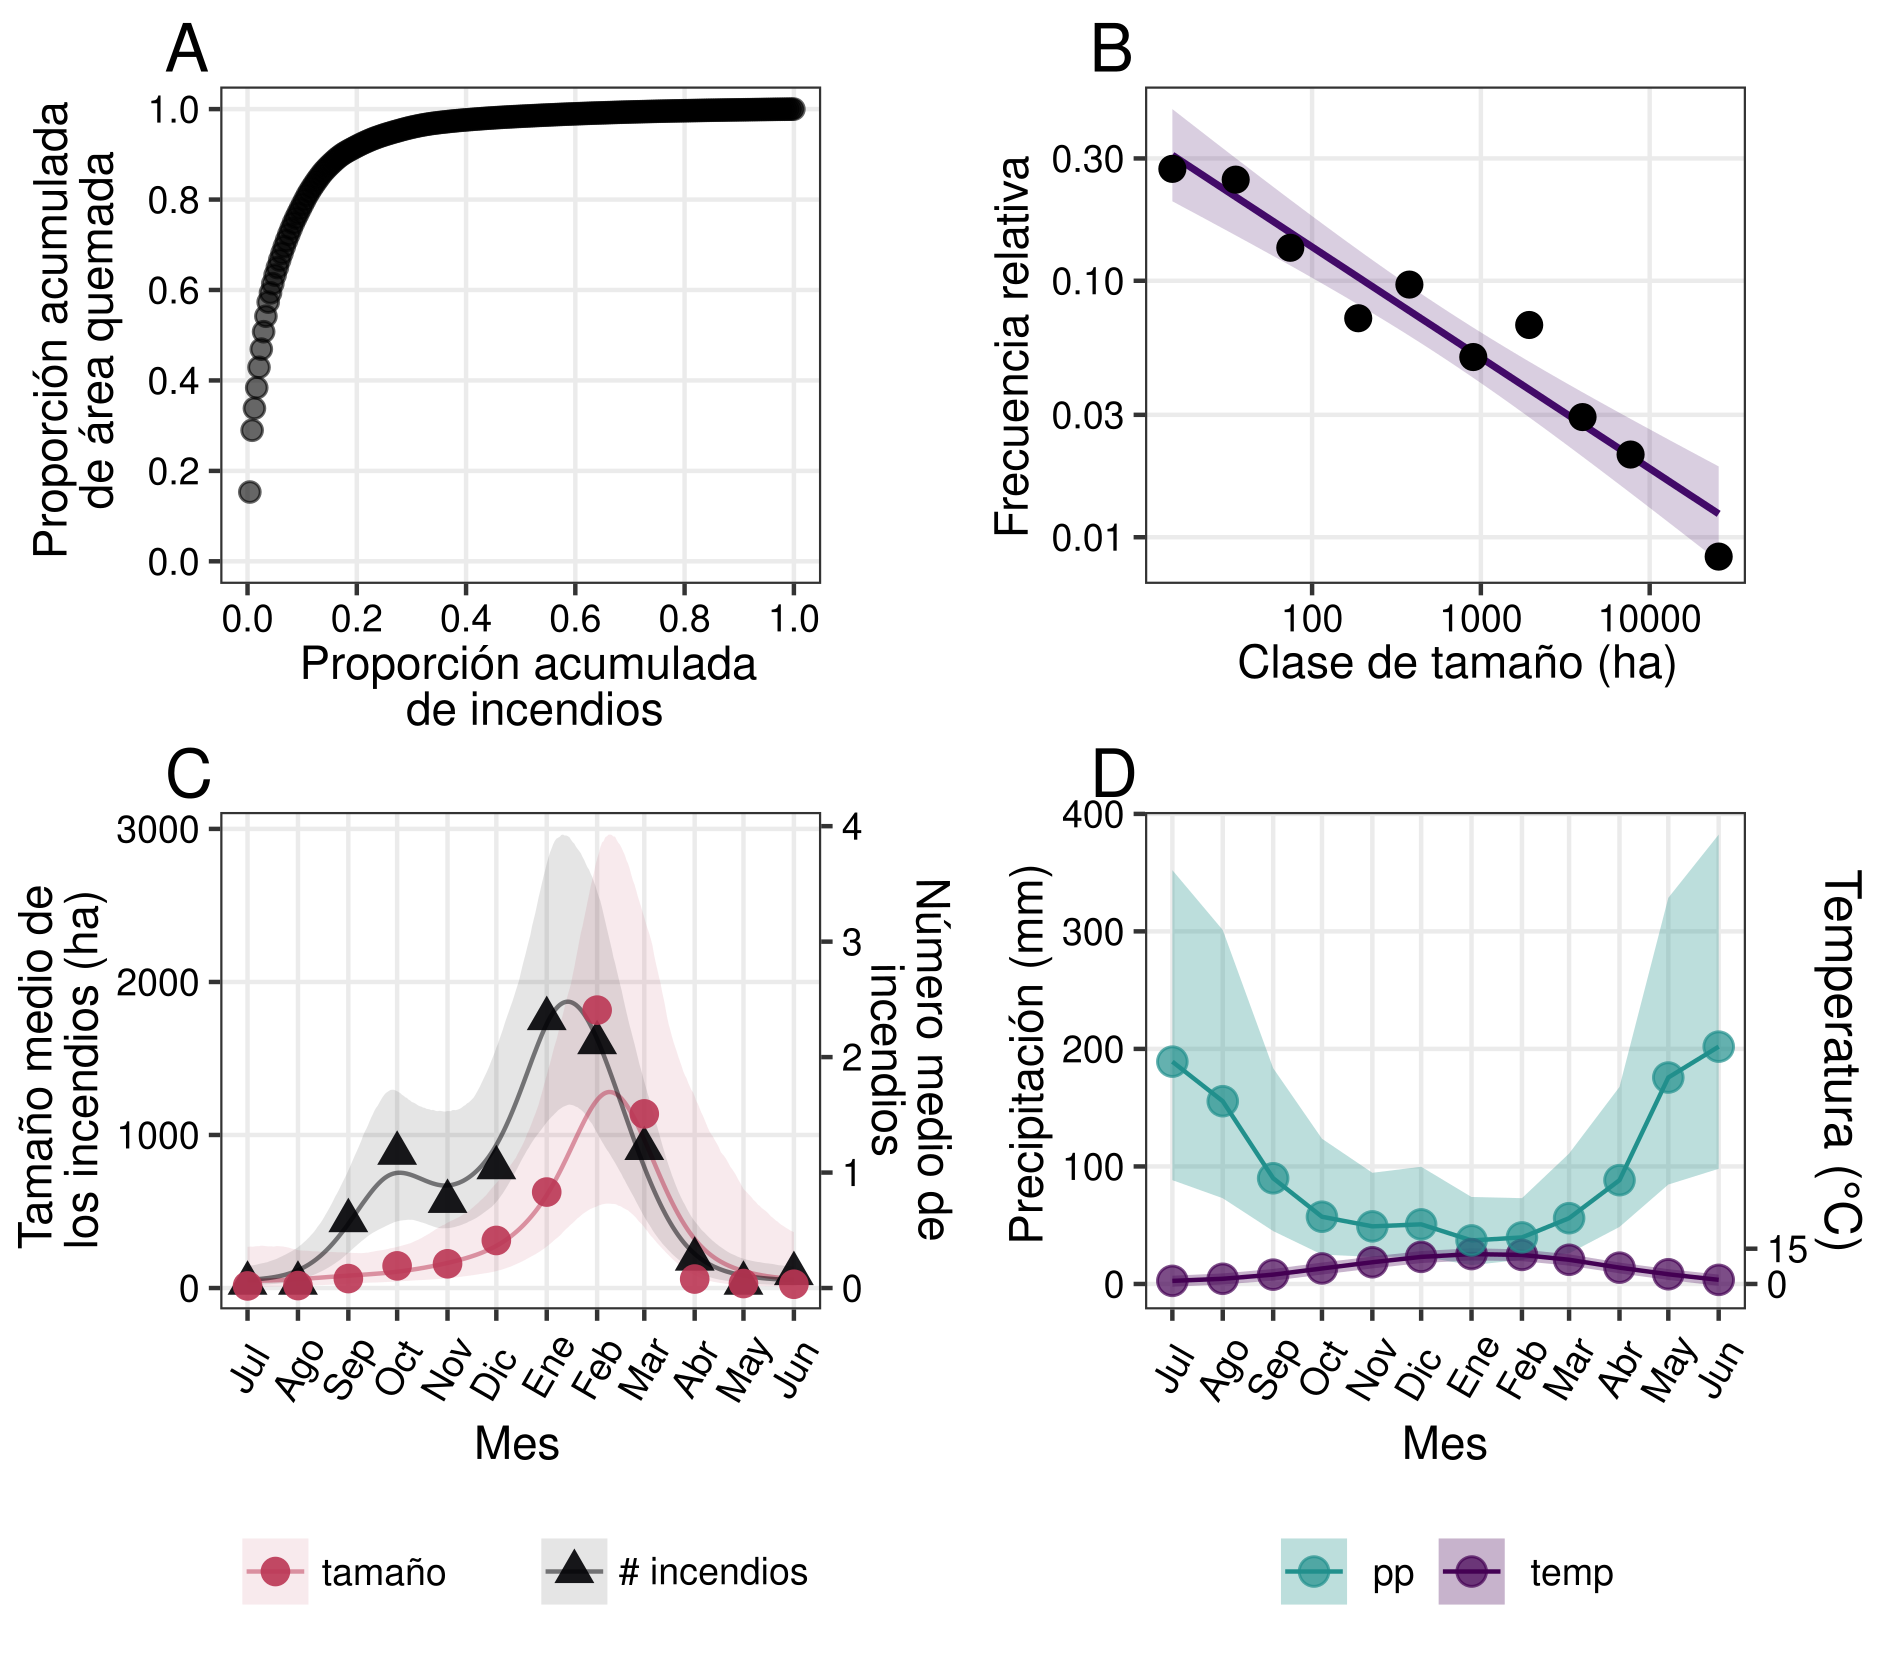
\includegraphics[width=16cm]{figuras/cap3/02) fire_regime.png}
    \caption[Distribución de tamaños y estacionalidad de incendios.]{(A) Proporción acumulada del área quemada en función de la proporción acumulada de incendios, ordenados de mayor a menor. (B) Frecuencia relativa de incendios por clase de tamaño (ambas variables en escala $\text{log}_{10}$). La línea y la banda muestran la media y el intervalo de confianza (IC) del 95 \% de una regresión lineal. (C) Tamaño promedio de los incendios y número de incendios por año y mes, promediados en los 24 años. Las curvas y bandas muestran la media y el IC del 95 \% estimados por los GAM, para un año promedio. (D) Precipitación y temperatura mensuales promedio, resumidas en todo el área de estudio con la media (puntos) y los percentiles 5 \% y 95 \% (bandas). Las líneas conectan los puntos solo para mejorar la visibilidad.} 
    \label{fig:cap3-02}
\end{figure}

\FloatBarrier

\subsection{Patrones temporales interanuales: incidencia del fuego en función de las variaciones climáticas}

Entre 1999 y 2022, la proporción anual promedio quemada en relación al área quemable fue del 0.25 \% (5400 ha), variando mayormente entre el 0.001 \% (21.24 ha) y el 0.78 \% (17144 ha), con un valor extremo del 2.04 \% (44578 ha) en 2015 (Fig.~\ref{fig:cap3-03}A). El número anual de incendios varió entre 1 y 28, con una media de 9.92. La proporción quemada anual y el número de incendios mostraron una ligera tendencia creciente con el tiempo, aunque con alta incertidumbre y elevados valores P (0.34 y 0.63, respectivamente; Tabla~\ref{tab:climate-ts}). Por el contrario, las variables climáticas mostraron claras tendencias hacia veranos más secos y cálidos, generalmente con valores P bajos (Tabla~\ref{tab:climate-ts}).

La proporción quemada anual y el número de incendios mostraron una variación clara en función de las variables climáticas, con valores de $\text{R}^2$ que oscilaron entre el 32 \% y el 60 \% (Fig.~\ref{fig:cap3-03}B). Ambas variables aumentaron con la temperatura, el déficit de presión de vapor y el FWI, y disminuyeron con la precipitación (Fig.~\ref{fig:cap3-03}B). La proporción quemada anual mostró una respuesta lineal a la temperatura, la precipitación y el FWI en escala logarítmica (lo que implica una respuesta exponencial en la escala original), pero el déficit de presión de vapor mostró un efecto de saturación (Fig.~\ref{fig:cap3-03}B). El número de incendios mostró una respuesta de saturación a todas las predictoras, excepto para el FWI, que produjo un efecto aproximadamente exponencial (Fig.~\ref{fig:cap3-03}B). Sin embargo, los efectos de saturación del déficit de presión de vapor sobre la proporción quemada anual (en $\text{log}_{10}$) y el número de incendios estuvieron fuertemente influenciados por el año 2022, que mostró el déficit de presión de vapor más alto, escasos incendios y una proporción quemada moderada (Fig.~\ref{fig:cap3-03}B).

\begin{figure}[htbp]
    \centering
    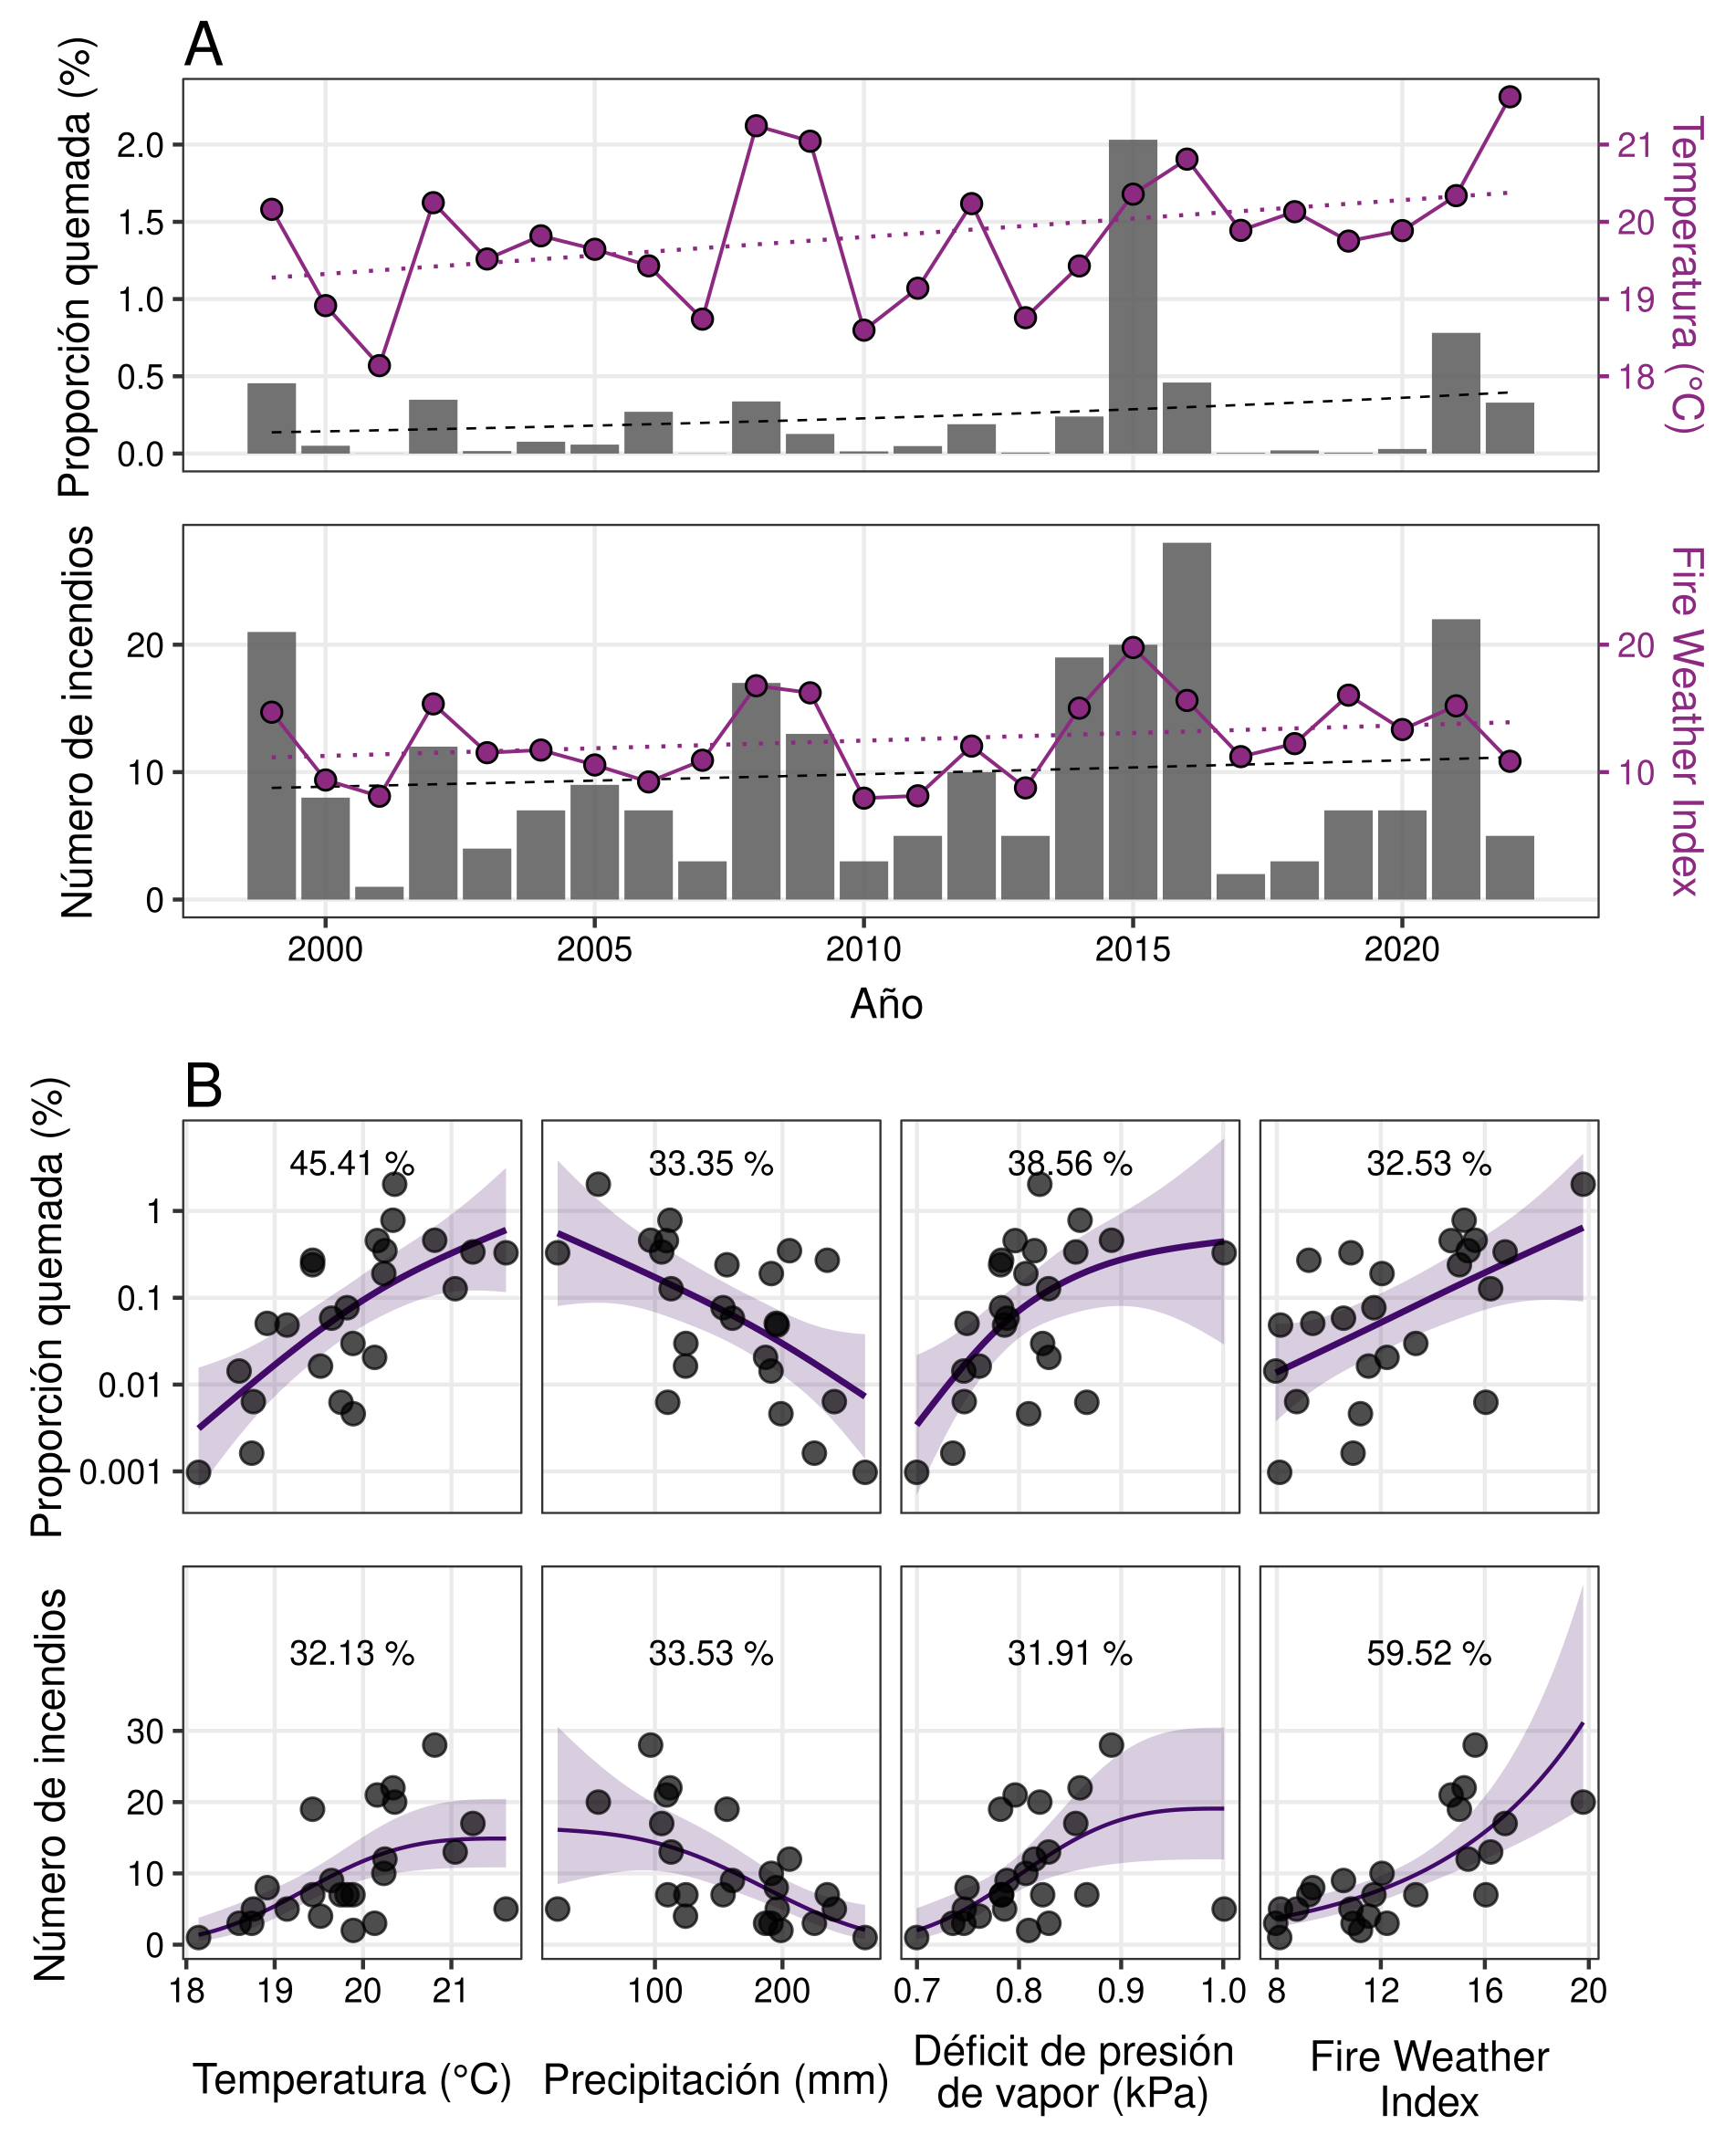
\includegraphics[width=16cm]{figuras/cap3/03) temporal_trends.png}
    \caption[Patrones temporales interanuales en la incidencia del fuego.]{(A) Proporción quemada anual del paisaje (arriba) y número de incendios $\ge 10$ ha (abajo) por año (barras), junto con la serie temporal de la variable climática con mayor efecto (temperatura y Fire Weather Index, respectivamente; puntos y línea). Las líneas punteadas y discontinuas muestran la media predicha de los modelos de tendencia interanual ajustados a cada variable. (B) Proporción quemada anual (arriba, en escala $\text{log}_{10}$) y número de incendios $\ge 10$ ha (abajo) en función de variables climáticas por año, promediadas entre diciembre y marzo. Las curvas y bandas muestran las medias estimadas por los GAM con restricciones de forma y sus IC del 95 \%. Los números dentro de los paneles muestran los valores de $\text{R}^2$ bayesiano (\%;  \citealt{gelman_r-squared_2019}).} 
    \label{fig:cap3-03}
\end{figure}

\begin{table}[ht]
\centering
\caption[Tendencias temporales en incidencia del fuego y variables climáticas.]{Proporción quemada y número de incendios por año y variables climáticas (promediadas durante la temporada de incendios) en función del tiempo (con el año como única predictora). Los modelos de proporción quemada y número de incendios fueron ajustados con un enlace logarítmico, por lo que $\exp{(\beta)}$ representa el factor de aumento anual. Las pendientes restantes son las tasas de cambio anual en la escala de la respuesta (enlace identidad). Los valores de $\text{R}^2$ bayesiano se muestran en la última columna \citep{gelman_r-squared_2019}.}
\label{tab:climate-ts}
\begin{tabular}{lccccc}
\toprule
Variable respuesta & $\beta$ & Error estándar & t & P & $\text{R}^2$ (\%) \\
\midrule
Proporción quemada (\%)           & 0.046   & 0.047 & 0.976  & 0.340 & 8.616  \\
Número de incendios               & 0.011   & 0.022 & 0.491  & 0.624 & 1.032  \\
Temperatura ($^\circ$C)           & 0.048   & 0.024 & 1.992  & 0.059 & 14.716 \\
Precipitación (mm)                & -3.635  & 1.658 & -2.192 & 0.039 & 17.286 \\
Déficit de presión de vapor (kPa) & 0.006   & 0.001 & 3.924  & 0.001 & 40.098 \\
Fire Weather Index                & 0.120   & 0.094 & 1.273  & 0.216 & 6.582  \\
\bottomrule
\end{tabular}
\end{table}

\FloatBarrier

\subsection{Patrones espaciales: efectos de la vegetación, topografía, precipitación e influencia humana}

En el modelo ambiental, donde no se consideró el tipo de vegetación, la altitud y la precipitación fueron los controles físicos más fuertes sobre la probabilidad de quema, que fue mayor en áreas de baja altitud y precipitación (Fig.~\ref{fig:cap3-04}A.1 y \ref{fig:cap3-05}A.1). La probabilidad de quema también aumentó en pendientes pronunciadas orientadas al norte y disminuyó ligeramente con la posición topográfica (Fig.~\ref{fig:cap3-04}.1). Sin embargo, estas variables mostraron efectos menores. El NDVI mostró un efecto unimodal, con la mayor probabilidad de quema en valores intermedios (Fig.~\ref{fig:cap3-05}B.1). Las distancias a poblados y a caminos aumentaron considerablemente la probabilidad de quema, aunque sus efectos no se diferenciaron del azar (Fig.~\ref{fig:cap3-05}D.1).

En el modelo conjunto, que permite predecir los efectos de las variables ambientales por separado para cada tipo de vegetación, los efectos de la altitud y la pendiente se mantuvieron cualitativamente similares a los del modelo ambiental, pero variaron en magnitud. En la mayoría de los casos, el modelo ambiental mostró un tamaño de efecto intermedio. Esto sugiere que los efectos de la altitud y la pendiente se mantienen dentro de los tipos de vegetación, indicando que afectan el fuego directamente y no por su asociación con los tipos de vegetación. En los bosques húmedos y secos, la altitud mostró los mayores efectos sobre la probabilidad de quema, aunque con incertidumbre considerable en los bosques secos (P = 0.386). En los bosques subalpinos y matorrales, la altitud mostró efectos menores y esperables por azar (P = 0.776; Fig.~\ref{fig:cap3-04}A). El efecto positivo de la pendiente fue mayor en los matorrales y casi nulo en los pastizales (Fig.~\ref{fig:cap3-04}B). A diferencia de la altitud y la pendiente, el efecto de la orientación fue mayor en el modelo ambiental que dentro de los tipos de vegetación (modelo conjunto, Fig.~\ref{fig:cap3-04}C), lo que indica que la orientación afecta la probabilidad de quema al controlar la distribución de los tipos de vegetación (Fig.~\ref{fig:cap3-S01}). El efecto de la posición topográfica varió considerablemente entre los tipos de vegetación. Fue grande y positivo en los bosques húmedos y secos, aunque esperable por azar (P = 0.258). En los bosques subalpinos y pastizales, el efecto de la posición topográfica fue insignificante, y en los matorrales, fue pequeño y negativo (Fig.~\ref{fig:cap3-04}D).

La precipitación mostró un patrón similar al de la orientación: la disminución en la probabilidad de quema con la precipitación observada en el modelo ambiental se desdibujó en el modelo conjunto, donde se incluyeron los tipos de vegetación (Fig.~\ref{fig:cap3-05}A). Esto indica que el efecto de la precipitación observado cuando no se considera el tipo de vegetación se debe principalmente al recambio del  tipo de vegetación a lo largo del gradiente de precipitación (Fig.~\ref{fig:cap3-S01}). Dentro de los tipos de vegetación, el efecto de la precipitación solo fue claro en los bosques subalpinos, pero mostró una magnitud pequeña. En los bosques secos, el efecto fue mayor que en el modelo ambiental, pero esperable por azar. El NDVI mostró un efecto unimodal, evidente tanto en el modelo ambiental como dentro de la mayoría de los tipos de vegetación en el modelo conjunto (Fig.~\ref{fig:cap3-05}B). Este efecto fue mayor en los bosques húmedos, intermedio en los bosques subalpinos y menor en los pastizales y matorrales. En los bosques secos, el efecto del NDVI fue grande y negativo, pero esperable por azar (P = 0.424).

En el modelo conjunto, la distancia a caminos y a poblados mostró efectos positivos y de gran magnitud en algunos tipos de vegetación. Sin embargo, al igual que en el modelo ambiental, en ningún caso estos efectos se diferenciaron
estadísticamente del azar (Fig.~\ref{fig:cap3-05}D).

Los tipos de vegetación mostraron claras diferencias en la probabilidad de quema en el modelo de vegetación, que no incluyó variables ambientales (Fig.~\ref{fig:cap3-06}A). La probabilidad de quema fue mayor en los bosques secos, matorrales y plantaciones, y menor en los bosques subalpinos y praderas antrópicas. Sin embargo, las altas y bajas probabilidades de quema de las plantaciones y praderas antrópicas no se diferenciaron claramente del azar. Los bosques húmedos y pastizales mostraron probabilidades de quema intermedias (Fig.~\ref{fig:cap3-06}A).

Cuando se compararon los tipos de vegetación bajo las mismas condiciones ambientales utilizando el modelo conjunto, aún mostraron variaciones en la probabilidad de quema, pero con patrones diferentes respecto al modelo de vegetación, y con tamaños de efecto más pequeños y con mayor incertidumbre (comparar Fig.~\ref{fig:cap3-06}A con \ref{fig:cap3-06}C). Esto indica que las probabilidades de quema estimadas por el modelo de vegetación están influenciadas parcialmente por las condiciones ambientales contrastantes donde cada tipo de vegetación es más frecuente. Aunque los bosques subalpinos mostraron la menor probabilidad de quema cuando no se consideraron las variables ambientales (Fig.~\ref{fig:cap3-06}A), presentaron valores más cercanos al promedio cuando se compararon a iguales condiciones. Su probabilidad de quema fue mayor que en los bosques húmedos, similar a la de los pastizales y menor que en los matorrales (Fig.~\ref{fig:cap3-06}C.1 y \ref{fig:cap3-06}C.2). Los bosques secos, con la mayor probabilidad de quema en el modelo de vegetación, mostraron valores más bajos que los matorrales y similares a los pastizales cuando se compararon a iguales condiciones (Fig.~\ref{fig:cap3-06}C.3 y \ref{fig:cap3-06}C.4). Los bosques húmedos, con una probabilidad intermedia en el modelo de vegetación, mostraron el valor más bajo cuando se compararon a alta altitud, y un valor intermedio a baja altitud (Fig.~\ref{fig:cap3-06}C.2 y \ref{fig:cap3-06}C.4). Los matorrales mostraron la mayor probabilidad de quema bajo todas las condiciones, aunque con baja precipitación y altitud, los bosques secos y pastizales presentaron valores similares (Fig.~\ref{fig:cap3-06}C.3). Además, sus diferencias respecto al promedio mostraron valores P mayores que en el modelo de vegetación.

El modelo conjunto mostró el mayor poder explicativo ($\text{R}^2 = 12.73$ \%), seguido por el modelo ambiental ($\text{R}^2 = 8.36$ \%) y el modelo de vegetación ($\text{R}^2 = 1.51$ \%; Tabla~\ref{tab:cap3-spat-models}).

\begin{figure}[htbp]
    \centering
    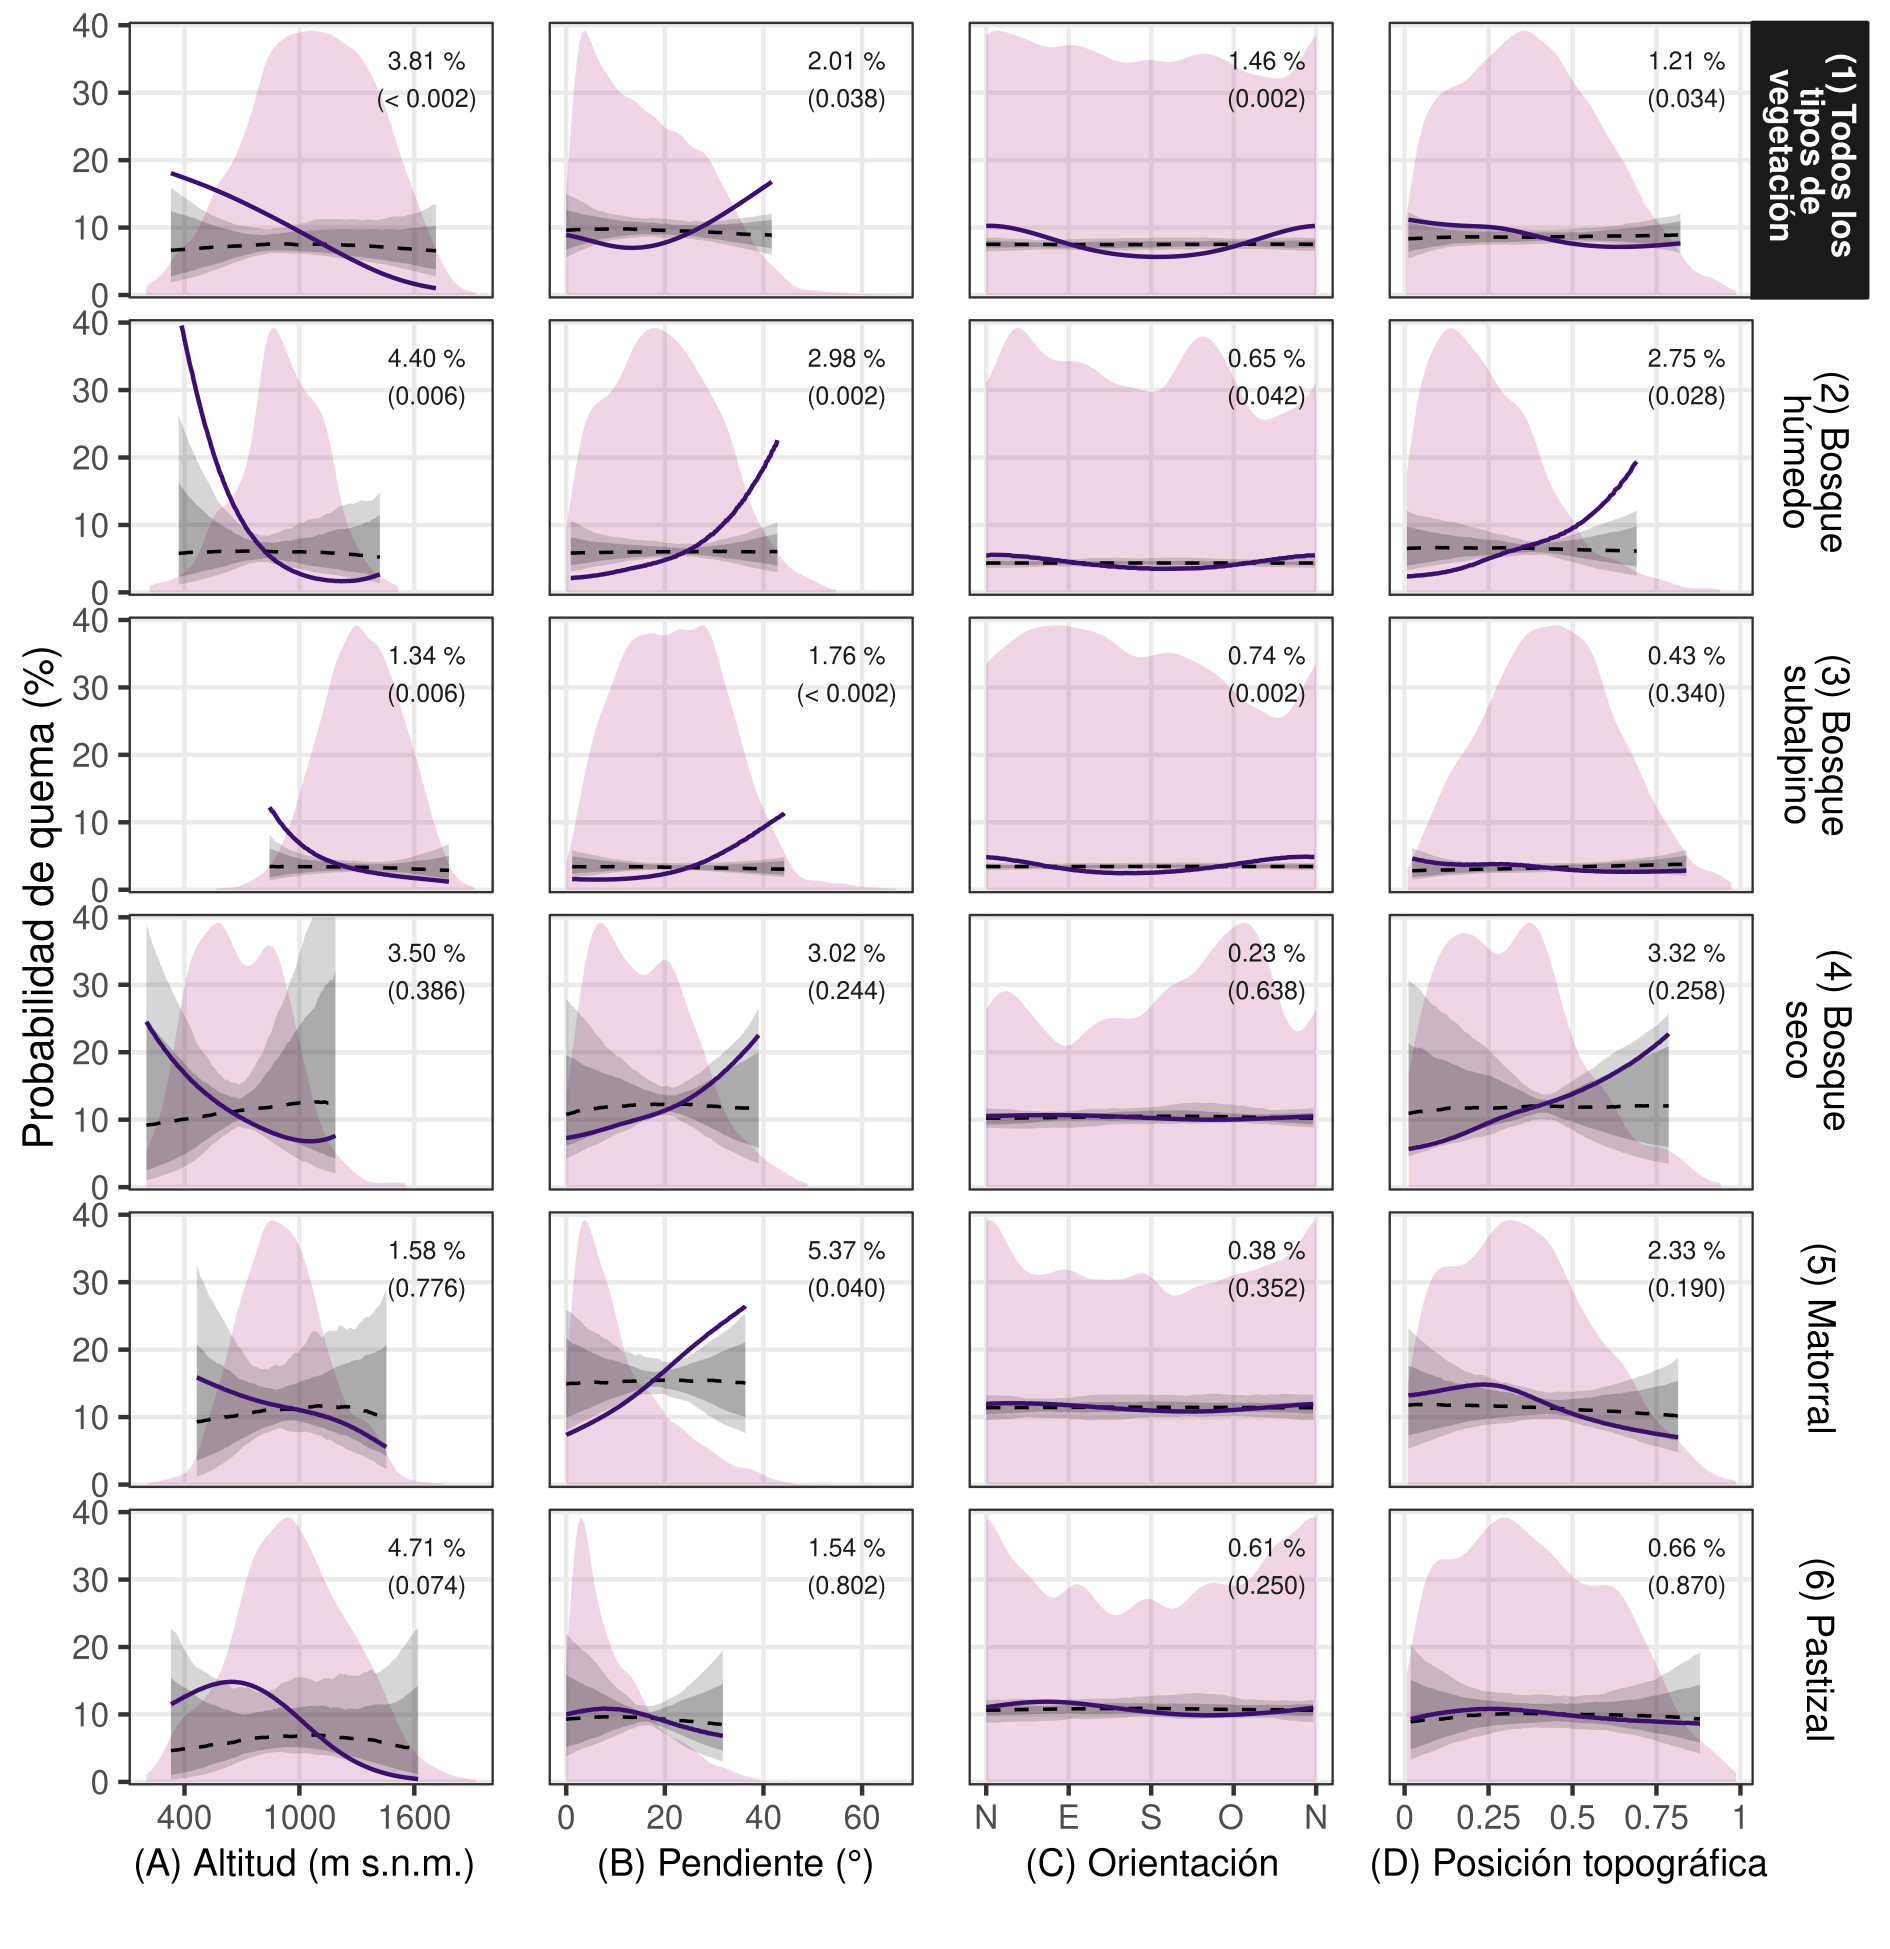
\includegraphics[width=16cm]{figuras/cap3/04) env_topo.png}
    \caption[Probabilidad de quema en función de variables topográficas.]{Probabilidad de quema en función de variables topográficas, predicha por el modelo ambiental, donde no se incluyó el tipo de vegetación (primera fila), y por el modelo conjunto, que incluye el tipo de vegetación (filas dos a seis). La línea sólida muestra la predicción de los modelos ajustados a los datos observados, mientras que las bandas grises y la línea discontinua muestran la distribución de la misma predicción obtenida a partir de modelos ajustados a datos aleatorizados (mediana e intervalos centrales de colas iguales con 80 \% y 95 \% de probabilidad). Las predicciones fueron calculadas a lo largo del intervalo de máxima densidad del 98 \% de cada predictora. Las sombras rosas muestran la distribución de la variable predictora. Los porcentajes dentro de los paneles indican el tamaño del efecto de cada predictora, con su correspondiente valor P.} 
    \label{fig:cap3-04}
\end{figure}

\begin{figure}[htbp]
    \centering
    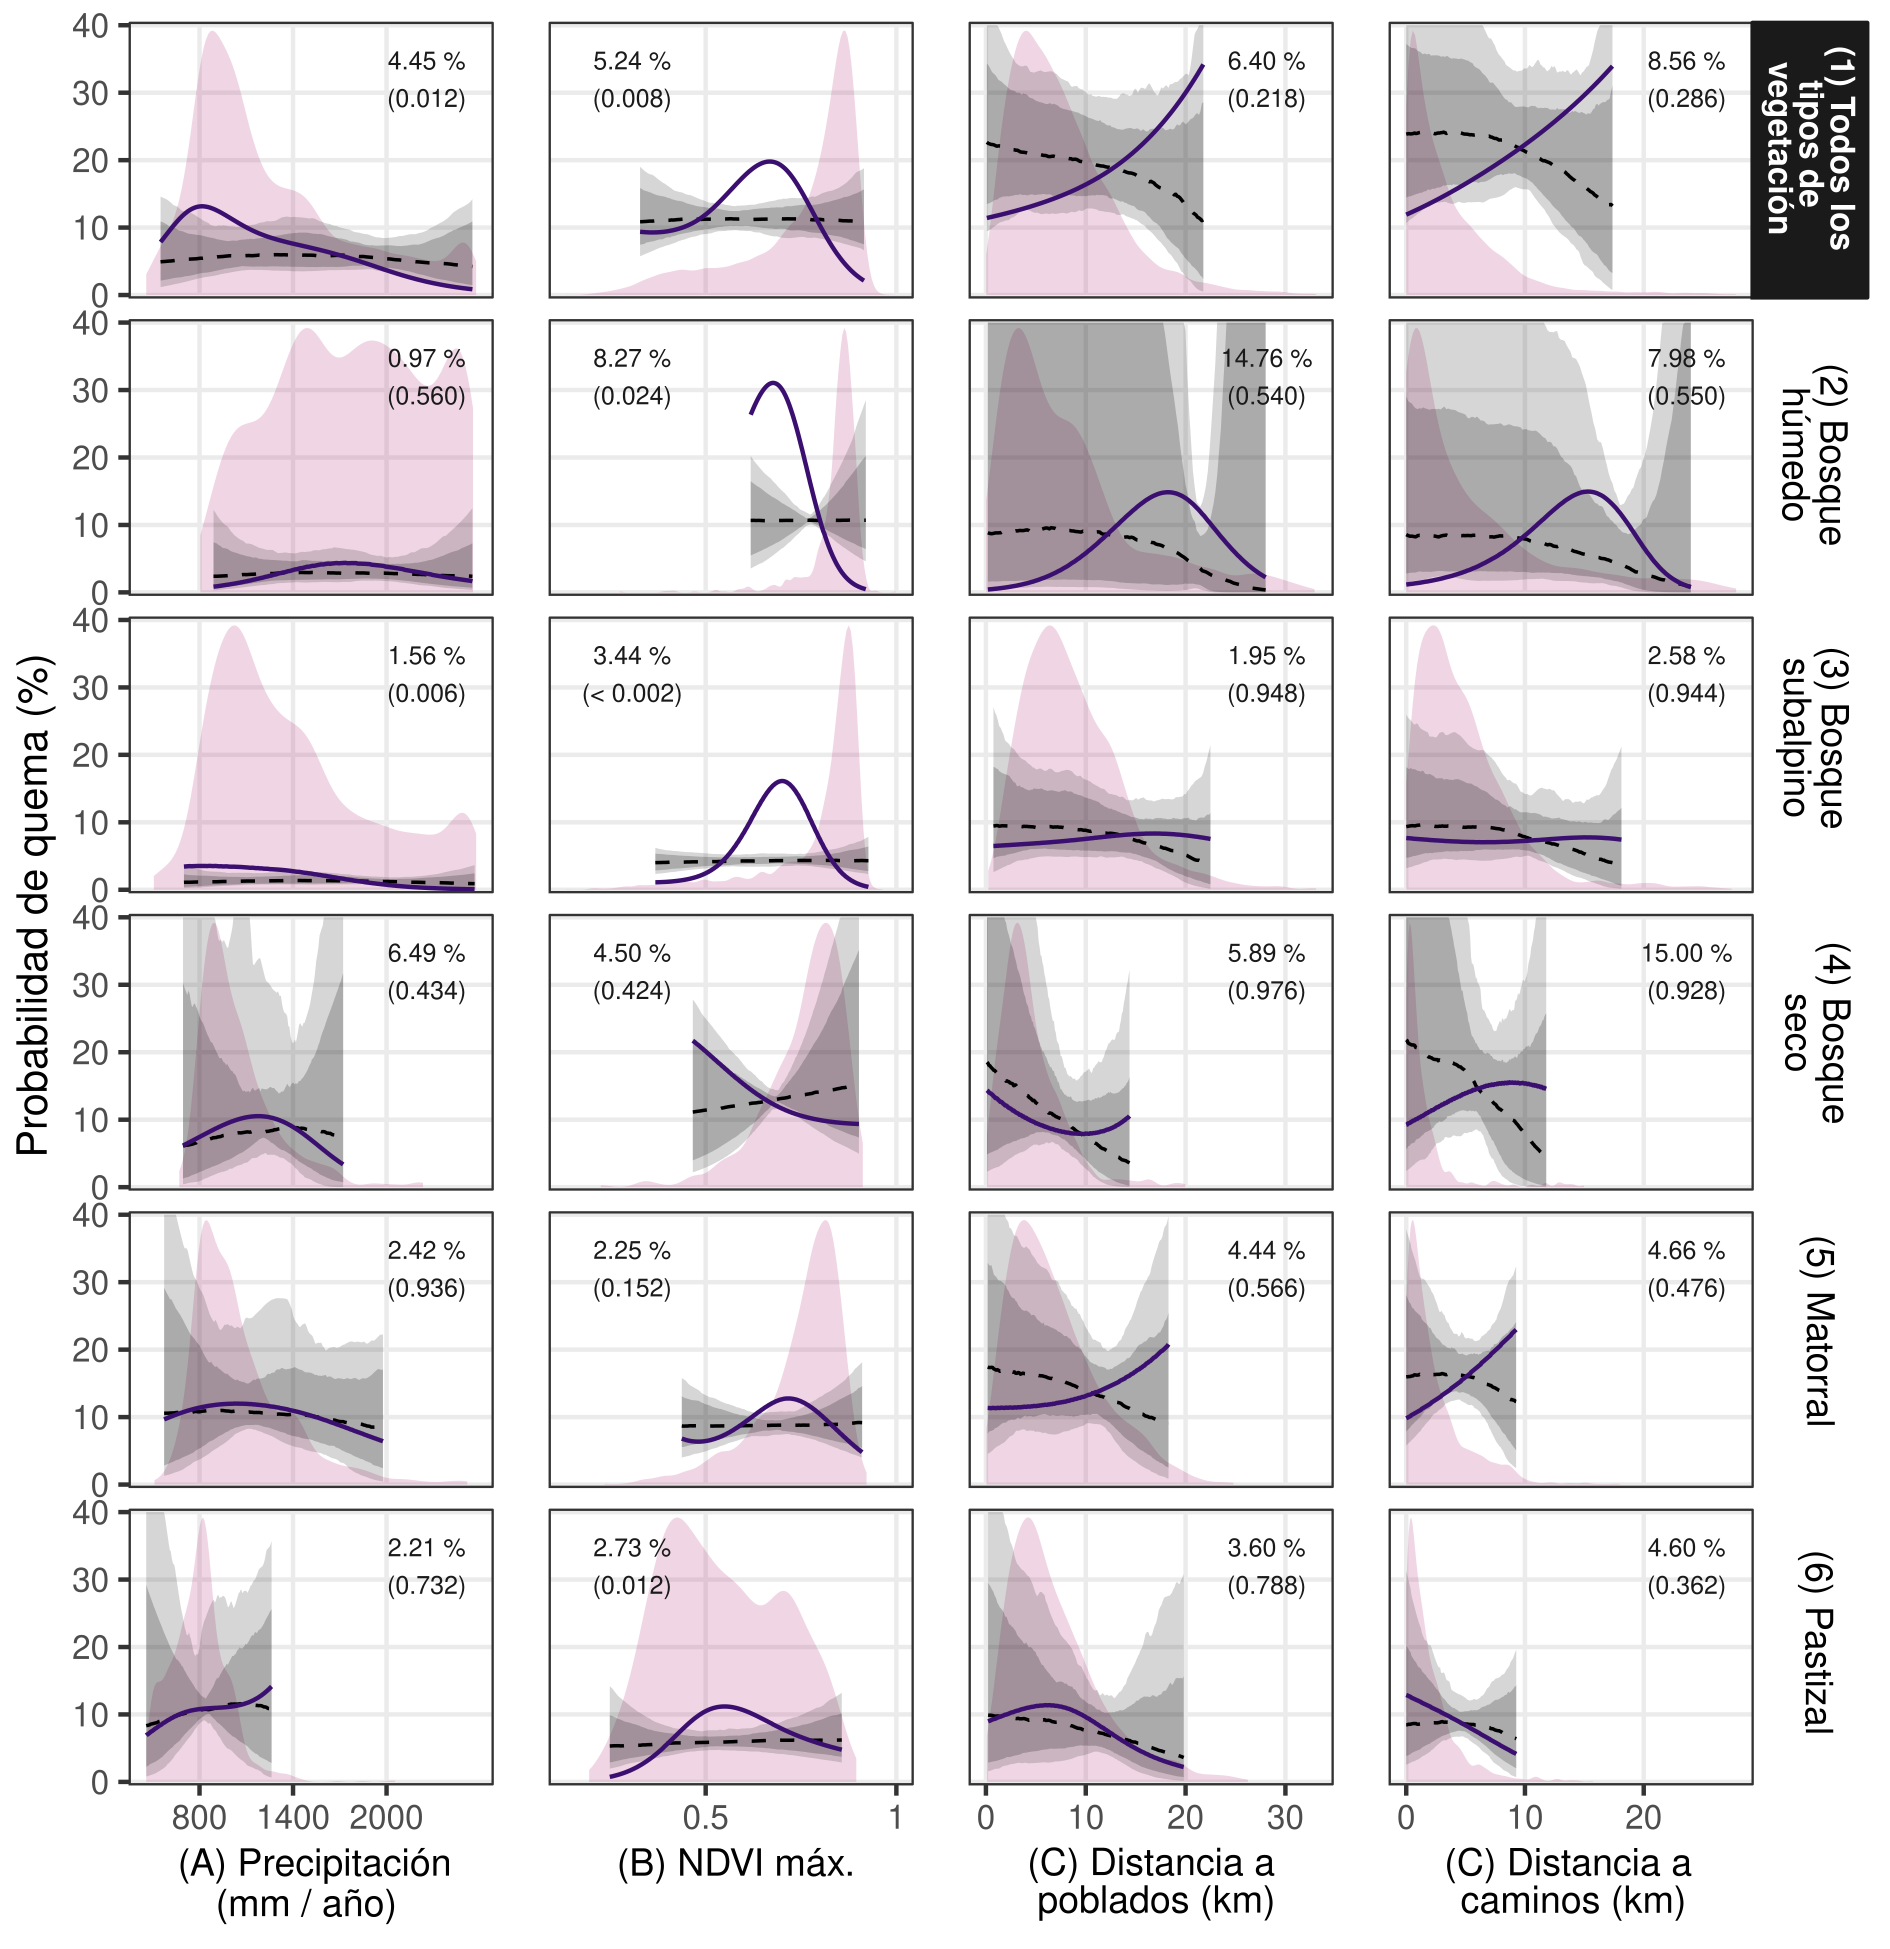
\includegraphics[width=16cm]{figuras/cap3/05) env_pp.png}
    \caption[Probabilidad de quema en función de la precipitación, el NDVI y la distancia a caminos y a poblados.]{Probabilidad de quema en función de la precipitación, el NDVI y la distancia a caminos y a poblados, predicha por el modelo ambiental, donde no se incluyó el tipo de vegetación (primera fila), y por el modelo conjunto, que incluye el tipo de vegetación (filas dos a seis). La línea sólida muestra la predicción de los modelos ajustados a los datos observados, mientras que las bandas grises y la línea discontinua muestran la distribución de la misma predicción obtenida a partir de modelos ajustados a datos aleatorizados (mediana e intervalos centrales de colas iguales con 80 \% y 95 \% de probabilidad). Las predicciones fueron calculadas a lo largo del intervalo de máxima densidad del 98 \% de cada predictora. Las sombras rosas muestran la distribución de la variable predictora. Los porcentajes dentro de los paneles indican el tamaño del efecto de cada predictora, con su correspondiente valor P.} 
    \label{fig:cap3-05}
\end{figure}

\begin{figure}[htbp]
    \centering
    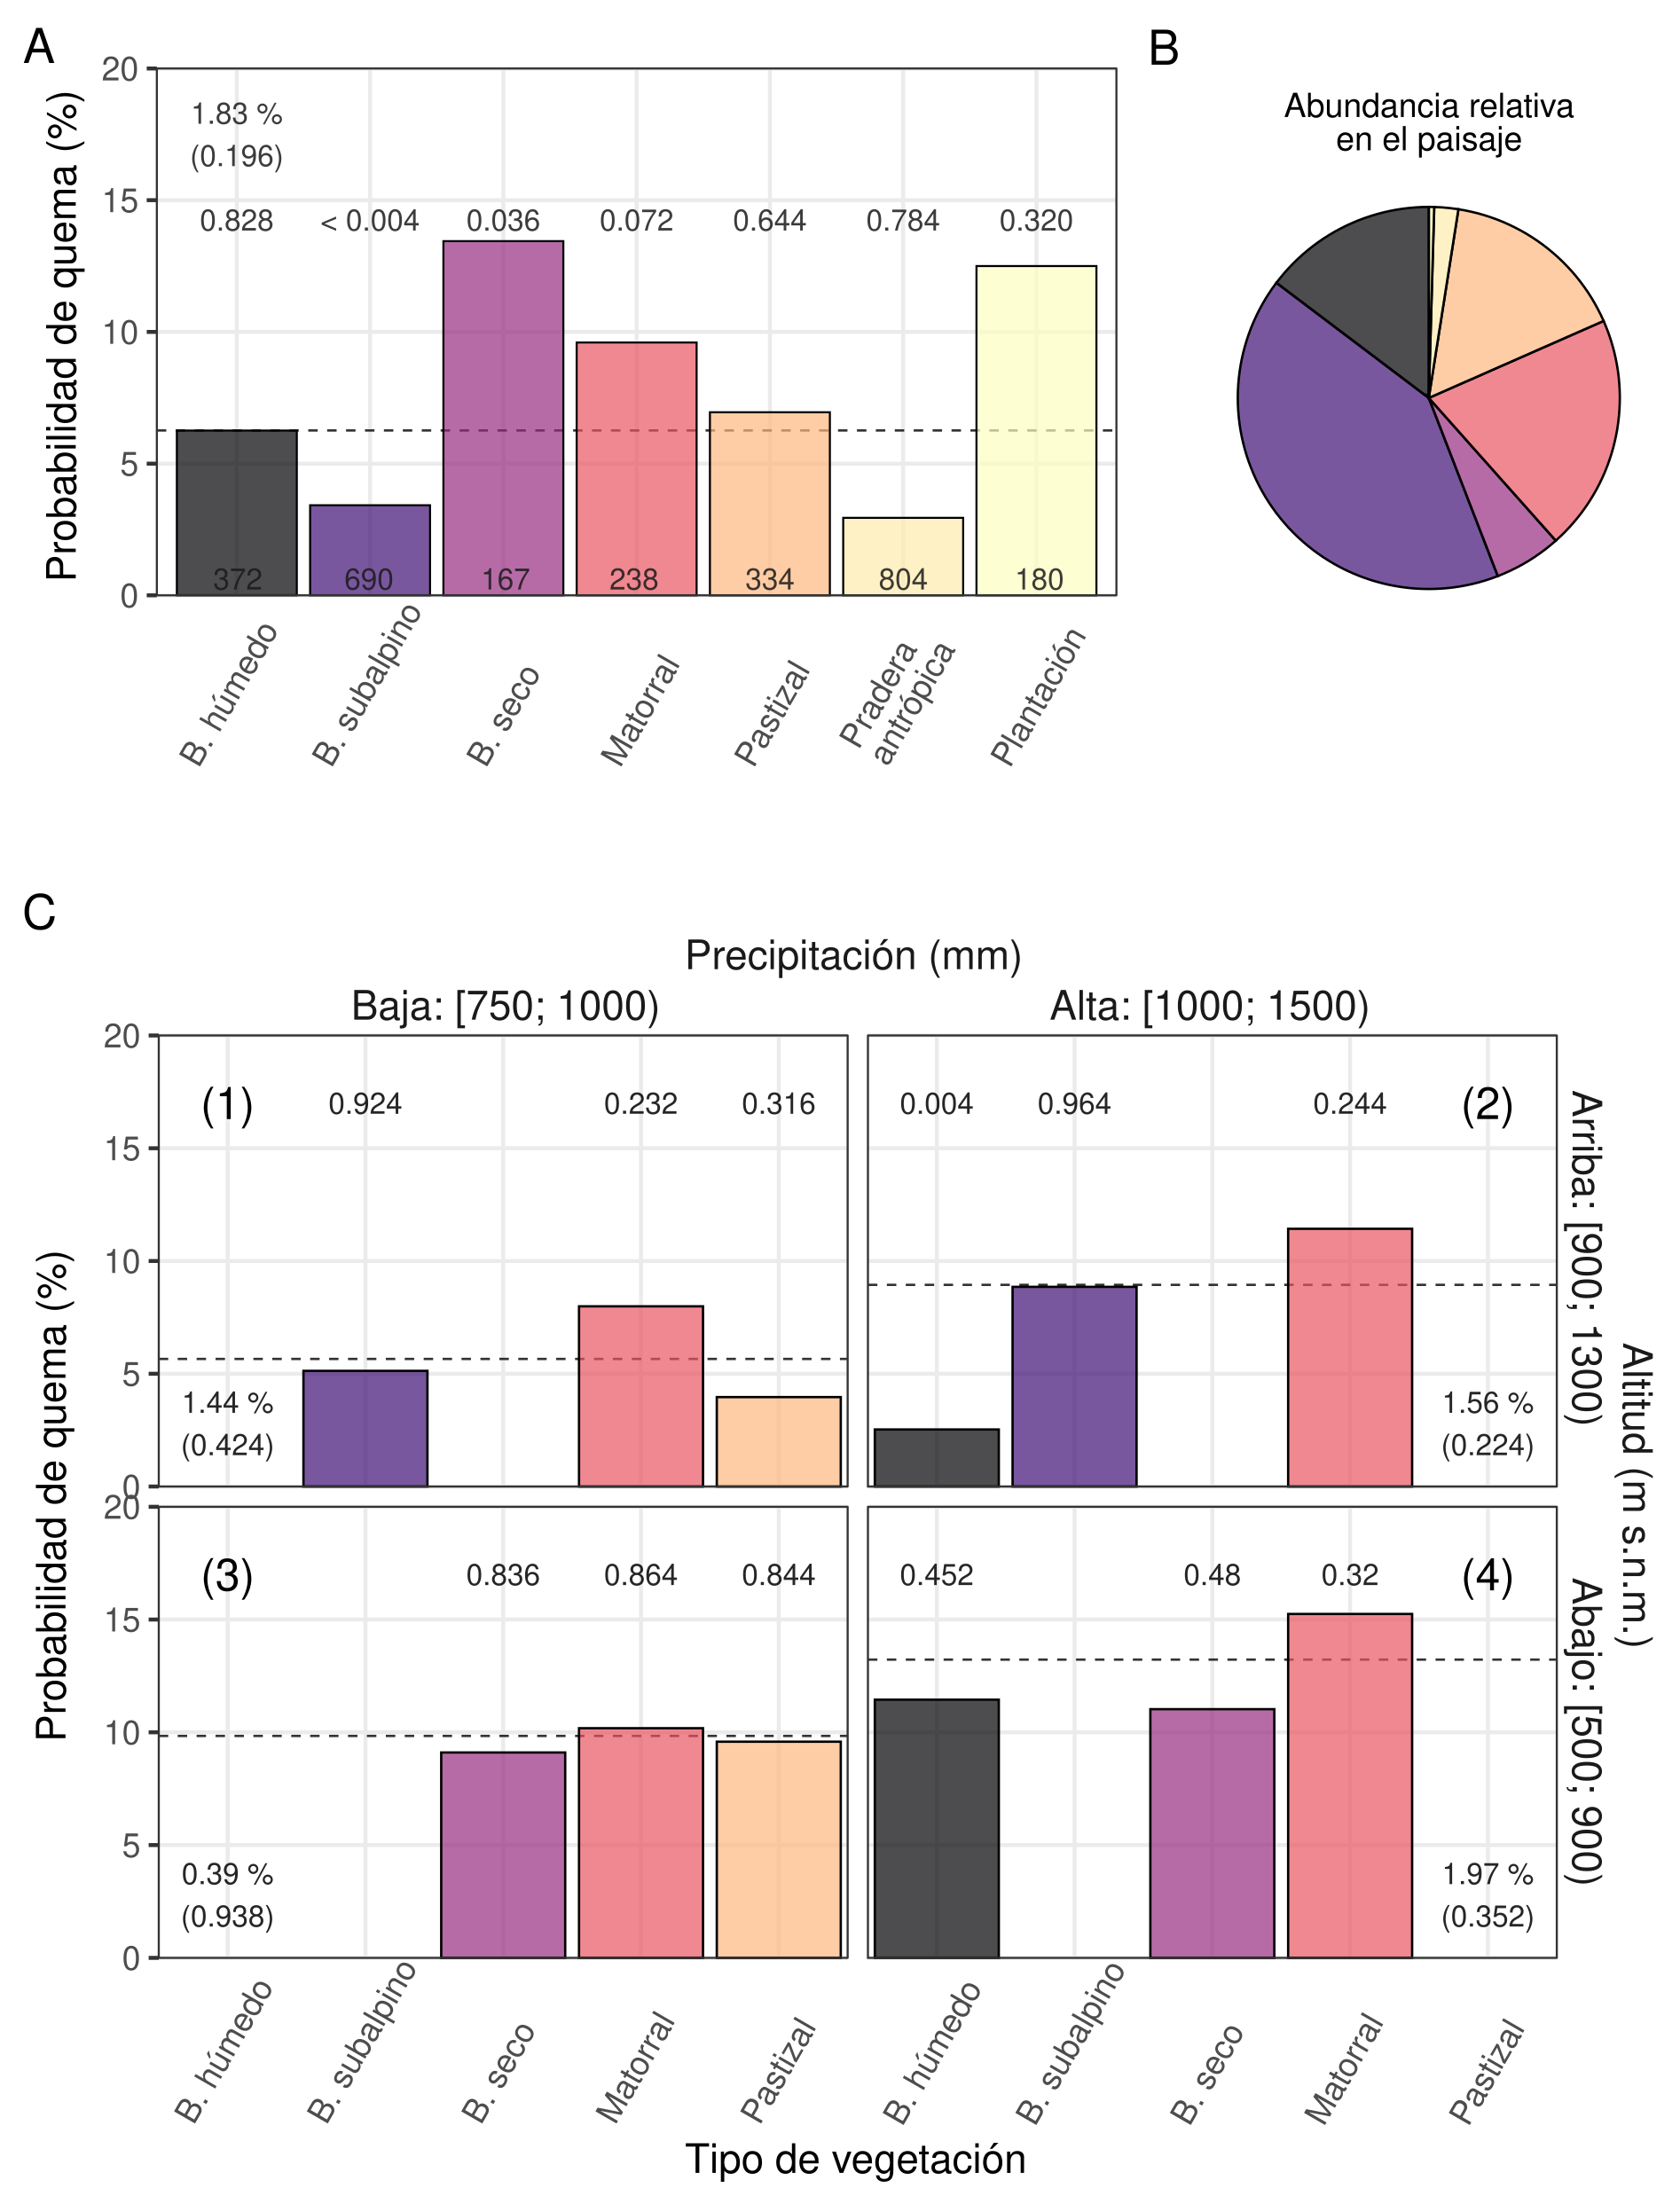
\includegraphics[width=16cm]{figuras/cap3/06) vegetation_v2.png}
    \caption[Probabilidad de quema en función del tipo de vegetación.]{(Leyenda en la página siguiente.)} 
    \label{fig:cap3-06}
\end{figure}

% leyenda en la página siguiente
\begin{figure}[p]
  \contcaption{(en la página anterior). (A) Probabilidad de quema en función del tipo de vegetación, predicha por el modelo de vegetación. En la base de las barras se indica el período de rotación ($PRF$, años), calculado a partir de la probabilidad de quema anual ($p_a$): $PRF = p_a^{-1}$. Dado que modelamos la probabilidad de que las celdas se quemaran al menos una vez en 24 años ($p_{24}$), obtuvimos la probabilidad de quema anual de la siguiente manera: $p_a = 1 - (1 - p_{24}) ^ {1/24}$. (B) Abundancia relativa de cada tipo de vegetación en el área quemable (las plantaciones casi no se distinguen por su baja representatividad en el paisaje). (C) Probabilidad de quema en función del tipo de vegetación, predicha por el modelo conjunto en cuatro condiciones ambientales, como un gráfico de dependencia parcial particionado (Apéndice~\ref{append:veg-comparison}). Algunos tipos no fueron graficados en condiciones ambientales donde es poco probable encontrarlos. En A y C, la línea horizontal discontinua muestra la probabilidad promedio de quema entre los tipos de vegetación ponderada por la abundancia relativa. Los números sobre las barras muestran los valores P a dos colas para las probabilidades de quema (Apéndice~\ref{append:pvalues}), y el porcentaje dentro de cada panel muestra el tamaño del efecto del tipo de vegetación con su correspondiente valor P (Apéndice~\ref{append:effsize}).} 
\end{figure}

% \FloatBarrier

\begin{table}[H]
\centering
\caption[$\text{R}^2$ de los modelos espaciales de probabilidad de quema.]{Valores de $\text{R}^2$ bayesiano \citep{gelman_r-squared_2019} para los tres modelos de probabilidad de quema y métricas de pruebas de razón de verosimilitud que comparan los modelos de vegetación y ambiental con el modelo conjunto. GL: grados de libertad.}
\label{tab:cap3-spat-models}
\begin{tabular}{lcccc}
\toprule
Modelo & $\text{R}^2$ (\%) & $\chi^2$ & GL & P \\
\midrule
Vegetación    & 1.51  & 677.65  & 67.532 & $<$ 2.2E-16 \\
Ambiental     & 8.36  & 249.01  & 56.583 & $<$ 2.2E-16 \\
Conjunto      & 12.73 & -       & -      & -           \\
\bottomrule
\end{tabular}
\end{table}


\FloatBarrier

\section{Discusión}

\subsection{Régimen de incendios}

La proporción quemada anual media, 0.25 \%, presenta una magnitud semejante a la reportada por estudios previos en la región, aunque es ligeramente superior: \citet{paritsis_habitat_2013} reportaron un 0.08 \% para el período 1984-2010, y los parques nacionales en nuestra área de estudio informan un 0.13 \% para el período 1938-1998 (\citealt{bruno_incendios_1982}; APN, datos no publicados). Aunque aparentemente alta y notablemente mayor a lo registrado para mediados del S. XX \citep{Gowda2012}, estos valores son notablemente menores a los estimados para fines del S. XIX y comienzos del S. XX, período en que los colonos euroamericanos usaban el fuego para abrir tierras para la cría de ganado \citep{veblen_historical_2008}. Según el análisis de Veblen et al. \citealt{veblen_historical_2008}, se estima que para el Parque Nacional Nahuel Huapi, entre 1890 y 1914 la tasa media de quema anual fue del 0.92 \%, en base a mapas de \citet{Willis1914}. A su vez, según mapas de \citet{Rothkugel1916}, en las provincias de Neuquén, Río Negro y Chubut, las zonas boscosas se quemaron en una tasa media de 1.48 \% anual en el mismo período. 

En relación a otras regiones, la proporción quemada anual media en nuestra área de estudio entre 1999 y 2022 es aproximadamente un orden de magnitud inferior a la reportada para las sierras del centro de Argentina (1.3-3.2 \%; \citealt{arganaraz_incidencia_2020}), para el Chaco Seco argentino (2.65 \%; \citeauthor{FerroChaco}, en revisión) y para áreas dominadas por coníferas en América del Norte (por ejemplo, 1.7 \%; \citealt{riddle2023wildfire}). La tasa de quema comparativamente baja que encontramos en esta región se asemeja a lo reportado en bosques de especies latifoliadas en el hemisferio norte, que presentan tasas de quema mucho más bajas que los bosques de coníferas \citep{marchal_turning_2020, foster_bottom-up_2022}.

La variación intraanual de la ocurrencia de incendios muestra que, aunque el área quemada alcanza su máximo durante el verano (enero-marzo), los incendios ocurren desde la primavera y aumentan su frecuencia en el verano. Los incendios frecuentes de mediados de verano (enero y febrero), iniciados por humanos o rayos, pueden eventualmente volverse grandes debido a la presencia de combustibles listos para arder (bajo contenido de humedad) combinados con condiciones climáticas que favorecen la propagación del fuego (máximo número de días consecutivos con alta temperatura, baja humedad y/o ausencia de lluvia). Los incendios de primavera, en su mayoría iniciados accidentalmente por humanos, tienden a permanecer pequeños debido a los altos niveles de humedad en la vegetación y condiciones climáticas menos favorables para la propagación del fuego \citep{barbera_microclimate_2023}. En nuestra área de estudio, el área quemada y el número de incendios disminuyen drásticamente cuando comienza el otoño, a pesar de la alta abundancia de especies caducifolias. Al parecer, la abundante precipitación en abril contrarresta los efectos del secado de los combustibles relacionado con la senescencia, lo que contrasta con otros bosques caducifolios que reciben menos precipitación en otoño (e.g., \citealt{tian_wildfires_2011}).

\subsection{Patrones temporales interanuales: incidencia del fuego en función de las variaciones climáticas}

Además del claro patrón estacional, también encontramos efectos marcados de la variabilidad climática interanual sobre la proporción quemada y el número de incendios, mostrando que la actividad del fuego aumenta en años con veranos más secos y cálidos \citep{kitzberger_climatic_1997, kitzberger_influences_1997, holz_ecological_2012, de_torres_curth_incendios_2008, kitzberger_projections_2022}. Otros estudios indican que este efecto se intensifica cuando las sequías comienzan desde el invierno anterior a la temporada de incendios, lo que sugiere un efecto acumulativo del déficit hídrico sobre la humedad del combustible \citep{kitzberger_climatic_1997, kitzberger_influences_1997, de_torres_curth_incendios_2008, kitzberger_projections_2022}. La mayor área quemada durante los veranos cálidos y secos se explica claramente por la humedad de los combustibles, pero dado que la incidencia de rayos aumenta bajo estas condiciones, una mayor tasa de ignición también podría contribuir a este patrón \citep{kitzberger_climatic_1997}. La variabilidad climática interanual también explica en gran medida los patrones de área quemada en otros bosques boreales y templados \citep{gill_top-down_2009, whitlock_past_2015, sommerfeld_patterns_2018, seidl_globally_2020, gaboriau_drivers_2022}.

A pesar del registro relativamente corto, encontramos una tenue tendencia al aumento en la proporción quemada y el número de incendios, similar al patrón encontrado en una serie temporal más larga. Aunque esta tendencia presentó un valor P alto, el aumento en la proporción quemada y el número de incendios coincide con una fase positiva proyectada para la Oscilación Antártica durante el siglo XXI \citep{thompson_signatures_2011}, lo que indica un cambio hacia un clima más favorable para los incendios, evidente también en nuestra serie climática, con una clara tendencia hacia veranos más cálidos y secos. Además, se espera que la probabilidad de incendios bajo escenarios de calentamiento global en el norte de la Patagonia Andina aumente entre 3 y 8 veces respecto a los valores actuales para fines de siglo, dependiendo del escenario climático \citep{kitzberger_projections_2022}. Asimismo, los efectos y tendencias climáticas encontrados en nuestro estudio coinciden con observaciones a nivel global, que asocian una mayor incidencia de incendios con el cambio climático \citep{wang_increasing_2015, robinne_global_2018, ellis_global_2022, lund_influence_2023}. Por lo tanto, la alta incertidumbre en la tendencia creciente de la proporción quemada anual probablemente sea resultado de un bajo poder estadístico. Esta tendencia probablemente se volverá estadísticamente más clara cuando se analicen más años. En particular, los análisis separados de las tendencias del área quemada por incendios causados por rayos y por humanos podrían ayudar a proyectar la incidencia del fuego, ya que ambas causas pueden responder de manera diferente al cambio climático y presentar desafíos contrastantes para el manejo. Se espera que la incidencia de rayos aumente en el norte de la Patagonia Andina con el cambio climático \citep{veblen_historical_2008} y, por lo tanto, la mayor parte del área quemada en el futuro podría ser causa de incendios por rayos, como se ha reportado en otras regiones \citep{miller2012trends, cattau2020anthropogenic}.

\subsection{Patrones espaciales: efectos de la vegetación, topografía, precipitación e influencia humana}

El tipo de vegetación y el entorno físico afectan la ocurrencia de incendios, pero comprender su influencia es desafiante porque el tipo de vegetación varía a lo largo de gradientes ambientales. Aunque estos efectos no pueden aislarse completamente con datos observacionales, nuestro estudio mejoró la comprensión de sus efectos separados sobre los incendios. Encontramos que, aunque la topografía determina en gran medida el tipo de vegetación en el norte de la Patagonia Andina, sus efectos más importantes sobre la actividad de incendios no pueden explicarse únicamente por la variación de los tipos de vegetación a lo largo de los gradientes topográficos. En cambio, la mayoría de sus efectos son evidentes dentro de los distintos tipos de vegetación. Por el contrario, la disminución de la ocurrencia de incendios en zonas de mayor precipitación y en laderas orientadas al sur se explica principalmente por cómo varían los tipos de vegetación con diferente cantidad y continuidad de combustible a lo largo de estos gradientes.

La marcada disminución de la probabilidad de quema con la altitud probablemente resulte de la reducción de la temperatura, lo que disminuye la evapotranspiración y retrasa el secado de los combustibles. De manera similar, la reducción de la probabilidad de quema en áreas con pendientes suaves y ubicadas en posiciones topográficas bajas puede explicarse por la mayor acumulación de agua y menor escorrentía en esos sitios. Dado que estas condiciones promueven una alta humedad de los combustibles, se espera que efectos similares de la topografía se encuentren en todos los tipos de vegetación. Además, las pendientes pronunciadas pueden quemarse más que las áreas planas porque favorecen la propagación del fuego cuesta arriba. Aunque las pendientes empinadas también podrían dificultar la propagación cuesta abajo, ese efecto parece ser menor que la facilitación de la propagación cuesta arriba, lo que explicaría por qué las áreas con mayor pendiente tienden a quemarse más. Este efecto también se espera que opere en todos los tipos de vegetación. Sin embargo, los efectos de la topografía mostraron cierta variación entre los tipos de vegetación. En algunos casos, esta variación se explica por el peso relativo de otras predictoras que covarían con la altitud, pero tienen efectos opuestos. Por ejemplo, en los pastizales, la pendiente y la posición topográfica no afectan la probabilidad de quema porque, al aumentar, también aumenta la altitud, contrarrestando sus efectos por disminuir la temperatura. Pero al controlar por altitud, la pendiente y la posición topográfica más alta aumentan la probabilidad de quema (Apéndice~\ref{append:cov}, Fig.~\ref{fig:cap3-S08}). Un fenómeno similar explica la baja importancia relativa de la altitud en los bosques subalpinos. A mayor altitud, las pendientes se vuelven más pronunciadas y el NDVI disminuye (Fig.~\ref{fig:cap3-S04} y \ref{fig:cap3-S07}A.3), contrarrestando el efecto de la menor temperatura sobre la probabilidad de quema. Nuevamente, al controlar por pendiente y NDVI, la altitud muestra un efecto importante en los bosques subalpinos (Fig.~\ref{fig:cap3-S08}). Sin embargo, en el caso de los matorrales, la baja importancia de la altitud no se explica por efectos contrapuestos de otras predictoras, sino probablemente por su fisonomía. Dado que presentan elevada cantidad y continuidad de combustible fino y un microclima que favorece el secado del combustible \citep{paritsis_positive_2015, tiribelli_changes_2018, barbera_microclimate_2023}, la menor temperatura a mayor altitud probablemente no reduzca tanto su inflamabilidad. Finalmente, los elevados valores P obtenidos para los efectos de la altitud en los bosques secos y matorrales probablemente resulten de la baja abundancia del primero y de la pequeña magnitud de efecto en el segundo, situaciones que reducen el poder estadístico.

A diferencia de los controles topográficos más importantes sobre el fuego, el efecto de la precipitación observado cuando no se consideraron los tipos de vegetación (en el modelo ambiental) parece explicarse principalmente por la variación en los tipos de vegetación a lo largo del gradiente de precipitación (Fig.~\ref{fig:cap3-S01}), y no tanto por cómo la precipitación afecta las condiciones del combustible dentro de los tipos de vegetación. La menor probabilidad de quema encontrada en áreas con alta precipitación probablemente se explique por la alta abundancia de bosques húmedos y subalpinos (Fig.~\ref{fig:cap3-S01}), que tienen baja continuidad vertical del combustible y un sotobosque con humedad intrínsecamente alta \citep{paritsis_positive_2015, tiribelli_changes_2018, barbera_microclimate_2023}. A medida que disminuye la precipitación, el aumento en la cobertura de matorrales parece incrementar la inflamabilidad, ya que presentan mayor cantidad y continuidad de combustible y menor humedad debido a la falta de un dosel cerrado. Sin embargo, en el rango más bajo de precipitación, por debajo de 800 mm / año, la precipitación parece afectar el fuego al controlar los combustibles dentro de los tipos de vegetación. En este rango, donde los pastizales son el tipo de vegetación dominante (Fig.~\ref{fig:cap3-S01}), la probabilidad de quema decae con la disminución de la precipitación (Fig.~\ref{fig:cap3-05}A.1). Por lo tanto, esa disminución en la probabilidad de quema ocurre porque los pastizales presentan menor productividad a baja precipitación (Fig.~\ref{fig:cap3-S07}E.6), y el fuego está limitado por la continuidad del combustible.

Encontramos que las diferencias en la probabilidad de quema entre los tipos de vegetación se explican tanto por su cantidad y continuidad de combustible contrastantes como por las condiciones topográficas donde cada uno es más abundante. La baja y alta probabilidad de quema encontradas en los bosques subalpinos y secos, respectivamente, cuando no se consideraron las predictoras ambientales, se explican en gran medida porque ocurren en los rangos de altitud más altos y más bajos. Al compararlos con otros tipos de vegetación a iguales condiciones, los bosques secos mostraron una probabilidad de quema relativamente baja, y los bosques subalpinos, valores intermedios. Para los bosques subalpinos esperábamos encontrar una probabilidad de quema similar a la de los bosques húmedos, debido a su similitud estructural, pero mostraron una probabilidad mayor. Esto podría explicarse por que las lengas presentan menor altura que los coihues, confiriendo una mayor continuidad vertical del combustible a los bosques subalpinos en comparación con los húmedos.

Nuestros resultados coinciden con la hipótesis de restricciones variables, donde las áreas de productividad intermedia muestran la mayor probabilidad de quema \citep{pausas_global_2013, krawchuk_constraints_2011}, en concordancia con \citet{kitzberger_projections_2022}. Este patrón también fue evidente dentro de los tipos de vegetación, y nuestros resultados sugieren que los bosques húmedos y subalpinos de baja productividad podrían presentar incluso mayor probabilidad de quema que los matorrales. Estos bosques con NDVI relativamente bajo ($\approx$~0.7) probablemente sean aquellos con doseles abiertos, donde la cantidad de combustible es alta y la humedad del combustible es baja. En los matorrales, el NDVI mostró efectos menores sobre la probabilidad de quema en comparación con la mayoría de los otros tipos de vegetación, lo que sugiere que, a pesar de presentar variabilidad en la cantidad y continuidad de combustible, rara vez alcanzan condiciones que reduzcan marcadamente la probabilidad de quema, ya que rara vez presentan doseles cerrados y altos. 

Dada la notable importancia de la productividad sobre la inflamabilidad de bosques y pastizales, será necesario evaluar cómo el cambio climático puede alterarla. En algunas regiones, el cambio climático aumenta la productividad debido a la mayor concentración de $\text{CO}_2$ atmosférico \citep{silva2013probing,sperlich2020gains}. Sin embargo, en esta región, es probable que el aumento de la temperatura y la disminución de la precipitación sobrecompense este efecto \citep{gutierrez2014increased}. Ante estas condiciones sería esperable que los bosques presenten mayor muerte parcial de copa, mortalidad, y que se vuelvan más abiertos  \citep{suarez2004factors,rodriguez2016influence,molowny2017changes}, lo que aumentaría su inflamabilidad. En caso de que el mismo proceso disminuya la productividad de los pastizales o de los bosques actualmente poco productivos, la inflamabilidad podría disminuir asociada a una menor continuidad del combustible.

A diferencia de los claros efectos de la vegetación y la topografía sobre la ocurrencia de incendios, encontramos un efecto poco claro de la distancia a poblados y a caminos. Sin embargo, el aumento en la probabilidad de quema a mayores distancias, aunque altamente esperado por azar, también podría resultar de incendios causados por rayos, que, al originarse lejos de poblados y caminos, presentan menor probabilidad de ser detectados y controlados. Estudios que analicen por separado las igniciones y la propagación del fuego, considerando la fuente de ignición (rayos vs. humanos), son necesarios para comprender mejor los efectos humanos sobre el fuego (e.g., \citealt{mundo_environmental_2013, morales_stochastic_2015, godoy_forty_2022}).

Nuestro análisis mejoró la comprensión de los efectos separados de la vegetación y las variables ambientales sobre el fuego, aunque reconocemos que este enfoque observacional no puede aislarlos completamente. Específicamente, nuestros resultados destacaron diferencias en la probabilidad de quema entre tipos de vegetación que probablemente sean el resultado de propiedades contrastantes del combustible (Fig.~\ref{fig:cap3-06}C) más que de la variación ambiental. Sin embargo, las diferencias observadas entre tipos de vegetación, incluso cuando se controlan los factores ambientales (Fig.~\ref{fig:cap3-06}C), podrían estar parcialmente influenciadas por variables ambientales no observadas (e.g., humedad del suelo). En general, nuestro estudio proporciona una base para investigaciones de campo más detalladas que permitan refinar nuestra comprensión de los controles del fuego relacionados con la vegetación y variables ambientales.

Los modelos de probabilidad de quema (de vegetación, ambiental y conjunto) presentaron valores de $R^2$ de muy bajos a bajos, lo cual resulta esperable considerando que sólo se utilizaron variables espaciales y no dinámicas. Que un píxel se queme o no depende fuertemente de que ocurra una ignición relativamente cerca o que el fuego propague desde un punto de ignición. Todo este proceso es altamente estocástico, dependiendo de variables meteorológicas y relaciones espaciales (e.g., dirección del viento en relación a las celdas receptora y dadora de fuego) que se resuelven a una escala espacial y temporal fina. Aún así, notamos que existe una marcada variabilidad espacial en la incidencia del fuego que podría ser explicada por variables espaciales asociadas al uso antrópico del territorio. La región Centro-Sur mostró la probabilidad de quema más alta, y la Norte, la más baja (Fig.~\ref{fig:cap3-01}A, Tabla~\ref{tab:cap3-spatvar}). Este patrón podrían ser explicado por diferencias en el manejo del fuego. Por ejemplo, las regiones Centro-Norte y Norte incluyen extensos parques nacionales (Nahuel Huapi y Lanín), en donde la menor incidencia del fuego podría explicarse por mayores esfuerzos de prevención y control. Futuros estudios considerando aspectos de manejo del fuego y otras variables de índole antrópico, como la densidad poblacional, contribuirán a entender mejor esta variabilidad regional. 

Otro aspecto a resaltar en relación a la variabilidad espacial en la incidencia del fuego es que nuestros resultados en cuanto a patrones espaciales pueden estar fuertemente influenciados por las zonas de mayor incidencia del fuego. En este trabajo suponemos los controles espaciales del fuego son similares entre regiones, ya que no tenemos evidencia para suponer diferencias muy marcadas entre ellas. A su vez, decidimos no analizar por separado cada región porque en nuestra área de estudio la incidencia del fuego es baja, y nuestro registro es relativamente acotado en el tiempo. En este contexto, pocos incendios pueden determinar los patrones obtenidos, por lo que se requiere compensar la baja incidencia del fuego y la corta serie temporal analizando grandes áreas. En caso de subdividir el análisis, los patrones se volverían menos confiables. La misma lógica aplica al análisis de la variabilidad interanual en la incidencia del fuego. Puede ocurrir que la tendencia no sea homogénea en el área de estudio, pero con las características de nuestra base de datos no resulta confiable analizar su variación espacial. A futuro, contando con series más largas, podremos analizar en mayor detalle cómo los controles del fuego y su tendencia temporal varían entre regiones.

\subsection{Implicancias para el manejo del fuego}

En ecosistemas donde la inflamabilidad aumenta con el tiempo desde el último incendio, como en los bosques de coníferas del hemisferio norte, los incendios frecuentes y de baja severidad limitan la ocurrencia de incendios extremadamente grandes y severos \citep{ryan_prescribed_2013}. Sin embargo, si (1) la inflamabilidad es mayor en los estadios sucesionales tempranos que en los tardíos, o (2) los tipos de vegetación resilientes al fuego son más inflamables que los sensibles al fuego, agregar fuego al sistema puede promover aún más incendios \citep{kitzberger_decreases_2012, tiribelli_non-additive_2019}. La vegetación del norte de la Patagonia Andina cumple con ambas condiciones. Los bosques, que en promedio son la comunidad menos inflamable, presentan mayor inflamabilidad en su estado sucesional temprano, y esta disminuye desde los 30 años luego de un incendio \citep{tiribelli_changes_2018, tiribelli_non-additive_2019, barbera_microclimate_2023}. A su vez, su regeneración posfuego es limitada \citep{cuevas_tree_2000, kitzberger_effects_2005, tercero-bucardo_field_2007, landesmann_importance_2018}. Los matorrales, más inflamables, persisten después del fuego y frecuentemente reemplazan a los bosques quemados \citep{kitzberger_firevegetation_2016, landesmann_increased_2021}. Estas dinámicas resultan en un ciclo donde el fuego frecuente promueve vegetación más inflamable, lo que a su vez promueve más incendios. Por lo tanto, para reducir los impactos del fuego en la sociedad y los ecosistemas, que se espera que aumenten con el cambio climático, es necesario limitar la ocurrencia de incendios tanto como sea posible.

Encontramos que las comunidades leñosas más productivas tienden a quemarse menos. Aunque la baja probabilidad de quema en áreas de alto NDVI puede deberse a la alta disponibilidad de agua relacionada con condiciones físicas a pequeña escala (e.g., alta humedad del suelo, menor insolación), esto también podría reflejar una estructura particular de la vegetación. Las áreas de alta productividad usualmente presentan doseles altos y cerrados, con sotobosques de escasa biomasa, baja continuidad vertical del combustible y/o alta humedad del combustible. Por lo tanto, promover el crecimiento de árboles altos para crear doseles cerrados que aumenten la humedad del combustible y reducir la cantidad y continuidad de los combustibles en los sotobosques podría reducir significativamente la inflamabilidad. Los doseles altos y cerrados pueden inducirse mediante prácticas de manejo de matorrales, como podar árboles cortos de múltiples tallos (como radales o ñires) para que tengan un solo fuste y así promover el crecimiento vertical, o plantar árboles de coihue, lenga y ciprés en la matriz de matorrales. Los combustibles en el sotobosque podrían reducirse combinando la extracción de leña y madera con la cría de ganado, que muestra un valor económico prometedor \citep{peri_review_2016, goldenberg_efecto_2018, goldenberg_shrubland_2021}. Sin embargo, dado que la humedad del combustible fino también puede disminuir con la cosecha, se necesitan estrategias cuidadosas para disminuir efectivamente la inflamabilidad \citep{goldenberg_effects_2020}. 

% Plantaciones: quitado por sugerencia de Grau, pero mencionar en Cap 5

%Otro aspecto a tener en cuenta en relación al manejo de la vegetación son las plantaciones e invasiones de coníferas exóticas. En la región, numerosas plantaciones de coníferas (\textit{Pinus ponderosa}, \textit{Pinus contorta}, \textit{Pseudotsuga menziesii} y \textit{Pinus radiata}) fueron establecidas desde la década de 1950, y careciendo de un manejo adecuado han acumulado una gran cantidad de combustible, volviéndose altamente inflamables \citep{SAGPyA2017}. A su vez, estas plantaciones son focos de invasión de ecosistemas nativos. Dada la mayor inflamabilidad de las plantaciones de coníferas y los sitios que invaden en comparación con las comunidades nativas \citep{paritsis_pine_2018, franzese_legacy_2022, cingolani2023enrichment}, realizar un manejo adecuado de las mismas mediante raleo y poda, y controlar las invasiones, es de gran importancia para reducir la inflamabilidad del paisaje \citep{gomez-gonzalez2024afforestation}. 

Pero más allá de las estrategias de manejo que pueden disminuir la inflamabilidad del paisaje, se espera que el clima futuro genere incendios que probablemente se propaguen incluso en estos entornos menos inflamables \citep{cawson_atmospheric_2024}, lo que pone en duda la eficacia de la gestión de combustibles como única estrategia. Por lo tanto, reducir las igniciones humanas y generar sistemas más efectivos de detección temprana de incendios podría ser la estrategia más efectiva para reducir la vulnerabilidad al fuego en esta región. Finalmente, las predicciones de modelos de propagación de incendios pueden ser útiles durante el proceso de supresión. Este estudio señala direcciones para mejorar el desempeño de los modelos de propagación recientemente desarrollados en la región \citep{morales_stochastic_2015, laneri_first_2020}, incorporando variables como altitud, NDVI y tipo de vegetación.

\subsection{Conclusiones}

Nuestros resultados confirman el fuerte efecto de la variación climática interanual en la ocurrencia de incendios en el norte de la Patagonia Andina, y también sugieren que el cambio climático aumentará la actividad de incendios, en concordancia con investigaciones previas \citep{kitzberger_projections_2022}. Espacialmente, encontramos que el efecto de la topografía en la ocurrencia de incendios no puede explicarse por la variación en los tipos de vegetación a lo largo de los gradientes topográficos. En cambio, la topografía probablemente afecta el fuego principalmente a través de su efecto en el balance hídrico y, por ende, en el contenido de humedad del combustible, con un efecto similar en todos los tipos de vegetación. Por el contrario, el efecto de la precipitación anual media en la incidencia del fuego se explica por la ocurrencia de tipos de vegetación con cantidad, continuidad y humedad de combustibles finos contrastantes a lo largo del gradiente.

Nuestra descripción de los patrones de área quemada para el inicio del siglo XXI puede servir como un punto de referencia para detectar cambios en el régimen de incendios en la región, y nuestro algoritmo de mapeo de incendios puede usarse para mantener este registro actualizado. Además, una mejor comprensión de cómo el fuego responde a factores biofísicos y humanos podría lograrse estudiando por separado la ignición y la propagación del fuego, para lo cual nuestros resultados y base de datos proporcionan un valioso punto de partida.

\section*{Disponibilidad de datos}

Los datos y el código para reproducir todos los análisis y figuras están alojados en GitHub (\url{https://github.com/barberaivan/patagonian_fires.git}).
\newpage{\ }
\cleardoublepage

\chapter[Capítulo 4. Modelando y proyectando el régimen de incendios en el norte de la Patagonia Andina]{Modelando y proyectando el régimen de incendios en el norte de la Patagonia Andina}\label{cap:modelos}

\section*{Resumen}

Con el clima volviéndose más propicio para la ocurrencia de grandes incendios, resulta fundamental desarrollar herramientas para proyectar cambios en el régimen de incendios a escala de paisaje. Sin embargo, la experimentación directa es impracticable en grandes extensiones y períodos prolongados, lo que hace que los modelos de simulación sean esenciales para explorar posibles trayectorias de los ecosistemas. 

En este capítulo desarrollamos un simulador del régimen de incendios para el norte de la Patagonia Andina, compuesto por tres modelos espacialmente explícitos: ignición, escape (comienzo de la propagación) y propagación. Los modelos fueron definidos en tiempo y espacio discretos, con resolución espacial de 30 m y temporal de 14 días. Las igniciones pueden ser causadas por rayos o por actividad humana; una vez iniciadas, pueden expandirse dependiendo de factores ambientales y espaciales. El modelo de propagación regula cómo el fuego se transmite entre celdas. En todos los modelos consideramos efectos de la topografía, la vegetación, el viento y las condiciones atmosféricas (mediante el Fire Weather Index). Los modelos de ignición y escape fueron ajustados con registros de focos ocurridos en el Parque Nacional Nahuel Huapi, y el de propagación, con los 235 incendios mapeados en un área más grande. 

Encontramos que el clima tiene un efecto determinante: mayores valores del Fire Weather Index aumentaron la probabilidad de ignición, escape y propagación. Integrando estos tres modelos proyectamos la incidencia del fuego en el Parque Nacional Nahuel Huapi para los períodos 2040-2049 y 2090-2099 bajo escenarios climáticos contrastantes. Las proyecciones indican que, para 2040-2049, la probabilidad de quema anual media aumentará en un factor de entre 2.07 y 2.61, subiendo desde el 0.1 \% actual a 0.2-0.25 \%. Para 2090-2099, se esperan aumentos en un factor de entre 1.36 y 31.17, dependiendo del escenario climático, lo que implica una probabilidad de quema anual de entre 0.13 y 2.97 \%.

\noindent \textbf{Palabras clave:} \textit{Ignición, escape, propagación, modelos, cambio climático.}

\section{Introducción}

Con el clima volviéndose más propicio para la ocurrencia de grandes incendios en muchas partes del mundo, resulta de gran importancia desarrollar herramientas que nos permitan predecir o proyectar cambios en el régimen de incendios a escala de paisaje \citep{senande2022spatial,bowman_vegetation_2020}. Sin embargo, predecir o proyectar procesos a escalas espaciales y temporales grandes es impracticable si pretendemos basarnos en datos experimentales, ya que no podemos manipular variables en grandes extensiones (e.g., miles de $\text{km}^2$) o por largos períodos de tiempo (e.g., décadas o siglos). Una herramienta clave para sortear esta limitación son los modelos de simulación. Representando un sistema de interés mediante modelos de simulación podemos explorar posibles trayectorias del mismo ante cambios en sus forzantes, a pesar de no poder evaluar dichos efectos experimentalmente \citep{brown2006landscape}. En ecología del paisaje se utilizan frecuentemente modelos dinámicos de vegetación, que representan la dinámica de la vegetación en interacción con disturbios, herbivoría, invasiones biológicas, manejo humano, y otros procesos de interés \citep{mladenoff2004landis, hartig2012connecting, turner2015landscape}. Integrando módulos de simulación de incendios en dichos modelos se pueden explorar posibles trayectorias de los ecosistemas ante un régimen de incendios alterado por cambio climático \citep{parisien2019applications}. Sin embargo, el desarrollo de modelos de simulación de incendios es desafiante, ya que existe un compromiso entre el detalle o precisión con que se representan los procesos y la disponibilidad de información para definir sus parámetros \citep{finney2005challenge}. 

Los modelos de simulación de incendios pueden ordenarse a lo largo de un gradiente de complejidad o detalle con el cual se representan los procesos \citep{sullivan2009wildland,papadopoulos2011comparative}. En el extremo más sencillo se sitúan modelos que no consideran explícitamente la ignición y propagación del fuego, sino que simplemente definen qué celdas del paisaje se queman, sin tomar información del vecindario. Un ejemplo de este tipo de modelo es el desarrollado por \citet{kitzberger_projections_2022}, o el modelo conjunto expuesto en el Capítulo~\ref{cap:patrones}, Sección~\ref{cap3:spat-analyses} \citep{barbera_patterns}. En general, cualquier modelo que devuelva una probabilidad o tasa de quema por unidad de tiempo para cada celda del paisaje puede utilizarse como un simulador de incendios rudimentario. En el otro extremo del gradiente se sitúan modelos con un elevado nivel de detalle, en donde se separan explícitamente la ignición y propagación del fuego, que en general requieren detallada información de los combustibles y las condiciones atmosféricas, ocurriendo a una resolución temporal subdiaria y cuya formulación busca representar procesos físicos al mayor detalle que sea manejable. Ejemplos de este tipo de modelos son FARSITE \citep{finney1998farsite}, FlamMap \citep{finney2006overview}, Phoenix \citep{tolhurst2008phoenix}, o Prometheus \citep{tymstra2010development}. Dónde uno se sitúa a lo largo de este gradiente depende principalmente de la disponibilidad de información para representar matemáticamente los procesos y definir los parámetros, y de la resolución espacial y/o temporal deseada \citep{sullivan2009wildland,papadopoulos2011comparative}. Cuando el objetivo es simular el avance de incendios reales para informar el combate, los modelos más detallados pueden ser de gran utilidad. Sin embargo, cuando el objetivo es evaluar potenciales trayectorias del ecosistema a una escala temporal de décadas, simuladores más simples y de menor costo computacional pueden resultar más convenientes. Por otro lado, a pesar de existir modelos muy detallados con gran eficiencia computacional \citep{finney2011method}, estos modelos requieren de información costosa de obtener, como carga y humedad de distintos tipos de combustible, o datos meteorológicos a escala horaria, ambos en grandes extensiones \citep{papadopoulos2011comparative}. Por estas limitaciones a veces resulta conveniente desarrollar modelos más sencillos que puedan utilizarse con la escasa información disponible en el sistema de interés (como mapas de vegetación e índices derivados de imágenes satelitales).

Debido a la baja resiliencia al fuego que presentan los bosques andino-patagónicos \citep{kitzberger_firevegetation_2016}, resulta de gran interés proyectar cambios en el régimen de incendios, y consecuentemente, en la representatividad de los bosques en el paisaje ante escenarios de cambio climático. En trabajos previos se han desarrollado modelos de simulación de incendios \citep{morales_stochastic_2015, laneri_first_2020}, algunos de los cuales fueron integrados en un modelo dinámico de vegetación (ver apéndices de \citealt{tiribelli_non-additive_2019} y \citealt{kitzberger_projections_2022}). El modelo de vegetación y los módulos de incendios están formulados en espacio y tiempo discretos, donde el paisaje se representa con una grilla de 60 m de resolución y las variables se actualizan en pasos anuales. Hasta el momento, el módulo de incendios consta de dos procesos con sus correspondientes modelos: un simulador de igniciones y un propagador de incendios \citep{morales_stochastic_2015}. El modelo de igniciones simula el número de igniciones por año y unidad de área, permitiendo considerar igniciones por rayos, con distribución espacial aleatoria, e igniciones humanas, con mayor probabilidad en cercanías de caminos y poblados. El modelo de propagación es un autómata celular, que simula el contagio de fuego entre celdas vecinas (vecindario de 8 celdas), donde la probabilidad de contagio depende del tipo de vegetación (bosque-matorral), la pendiente, la orientación de la ladera y la dirección del viento \citep{morales_stochastic_2015}. La variabilidad climática afecta únicamente al número de igniciones, pero no la propagación.

El objetivo de este trabajo fue avanzar el desarrollo de los modelos de simulación de incendios, e ilustrar su potencialidad proyectando el régimen de incendios bajo distintos escenarios de cambio climático para los períodos 2040-2049 y 2090-2099. En este contexto, nuestro objetivo no fue desarrollar un modelo para predecir con precisión incendios puntuales, sino explorar posibles cambios en el régimen de incendios, basándonos en numerosas simulaciones. Con respecto a las versiones anteriores, uno de los mayores cambios fue considerar el efecto de la variabilidad climática en todos los submodelos, y utilizar una resolución temporal sub-anual, de 14 días (quincena de ahora en más), que permite considerar dicha variabilidad de forma más realista. A su vez, integramos en la formulación de los modelos lo aprendido en el estudio de patrones de área quemada (Capítulo~\ref{cap:patrones}; \citealt{barbera_patterns}), representando los efectos de la vegetación y de variables físicas de una forma más adecuada a la vez que manteníamos un modesto número de parámetros a estimar. Desde un aspecto técnico, el mayor avance de este trabajo consta de la mejora del modelo de propagación, el cual presentó los mayores desafíos en términos estadísticos. Mientras que \citet{morales_stochastic_2015} estimaron dicho modelo utilizando sólo nueve incendios, en este caso utilizamos 57 incendios para estimar la mayor parte de los parámetros, y 235 incendios para un subconjunto menor. Esto fue posible gracias al mapeo sistemático de incendios realizado en el Capítulo~\ref{cap:patrones} (Apéndice~\ref{append:mapeo}) y la recopilación de puntos de ignición. 

\section{Métodos}

\subsection{Descripción general del enfoque de modelado}

El simulador de incendios fue definido mediante tres submodelos: ignición, escape, y propagación \citep{marchal_turning_2020}.  Este modelo (incluyendo sus tres submodelos) está diseñado para evaluar potenciales trayectorias del régimen de incendios a escalas temporales y espaciales grandes (décadas, algunos miles de km$^2$). En general, modelos como estos son llamados \textit{modelos de probabilidad de quema} \citep{parisien2019applications}. Estos modelos no buscan predecir al detalle incendios particulares, sino que intentan representar su potencial ocurrencia bajo una amplia variedad de condiciones, basándose en numerosas simulaciones \citep{parisien2020commentary}.

Formulamos los submodelos asumiendo tiempo y espacio discretos, representando el paisaje con una grilla rectangular con celdas de 30 m $\times$ 30 m, e intervalos de tiempo de 14 días. La ignición se define como el proceso por el cual el fuego comienza en una celda; el escape implica que dicha celda se queme por completo, pudiendo contagiar a las vecinas, y a partir de ahí, el contagio a las vecinas se rige por el modelo de propagación \citep{marchal_turning_2020}. Los módulos de fuego requieren de una capa de vegetación como entrada, pero no simulan la dinámica de la vegetación; únicamente pueden cambiar el estado de celdas quemables a quemadas. Para considerar retroalimentaciones entre fuego y vegetación, los simuladores de fuego deben acoplarse a un modelo dinámico de vegetación, que simule regeneración y sucesión. En el grupo de trabajo está previsto realizar esta integración como siguiente paso de modelado, pero en el presente trabajo nos limitamos a considerar una capa de vegetación estática; es decir, que se reinicia al estado inicial (quemable) cada año. Los años se centran en el verano, corriendo desde el primero de julio hasta el 30 de junio del siguiente año calendario, y son nombrados en base al mes en que terminan (e.g., el año 2014 corre desde el 01/07/2013 al 30/06/2014). Cada año consta de 26 quincenas, donde las primeras 13 transcurren desde el 31 de diciembre hacia atrás, y las 13 últimas, desde el 1 de enero hacia adelante (inclusive). Como los días de un año no son múltiplo de 14, los días restantes se agregan en la primera y última quincena. Como estas quincenas más largas se ubican en la estación húmeda, donde prácticamente no ocurren incendios, su mayor duración no afecta los procesos simulados. Las simulaciones de fuego fueron realizadas sobre el paisaje del Parque Nacional Nahuel Huapi (PNNH, Fig.~\ref{fig:pnnh_landscape}). 

En base a la limitada información que contenían los datos en relación a la complejidad de los procesos a modelar, optamos por formular modelos relativamente sencillos, procurando utilizar una baja cantidad de parámetros. Esto era particularmente necesario en el caso del modelo de propagación, ya que careciendo de datos sobre propagación requeríamos usar técnicas de alto costo computacional. A su vez, aportamos considerable información previa a los modelos, tanto a través de las funciones escogidas para modelar los procesos como restringiendo los valores de los parámetros. Con esta estrategia de modelado se requiere cierto cuidado a la hora de interpretar los resultados, ya que gran parte de ellos simplemente refleja supuestos previos, no información provista por de los datos. Por ejemplo, muchos parámetros están restringidos en su signo (e.g., sólo pueden tomar valores positivos), con lo cual, los datos informan únicamente su magnitud. Para estimar los modelos utilizamos inferencia Bayesiana, que permite incorporar información previa con gran flexibilidad y caracterizar la incertidumbre de los parámetros estimados mediante una distribución de probabilidad (distribución posterior; \citealt{gelman2013bayesian}). 

\subsection{Fuentes de datos}\label{cap4:data}

Para estimar los modelos de ignición y escape utilizamos la base de datos de focos del Parque Nacional Nahuel Huapi (PNNH), confeccionada por el equipo técnico del Departamento de Incendios, Comunicaciones y Emergencias (ICE), provista por Marcelo Bari. Esta base de datos registra las coordenadas y fecha de todos los focos registrados en el parque entre 1998 y 2021. Además, completamos este registro con la base de datos de incendios causados por rayos de \citeauthor{kitzbergerLightning} (en revisión), que abarca el período 1999-2023. Además de las coordenadas y fecha de cada foco, estas bases definen la causa (humana vs. rayo) y el tamaño final del incendio (incluyendo focos que no propagaron; Fig.~\ref{fig:pnnh_landscape}).

Para estimar el modelo de propagación utilizamos los incendios mapeados en el Capítulo~\ref{cap:patrones} (\ref{append:mapeo}). En este caso se requería conocer el punto de ignición de los incendios, y pudimos obtenerlo para 57 casos, que fueron provistos, en su mayoría, por Marcelo Bari (ICE-PNNH), otros, por personal de la Brigada de Puerto Patriada del Servicio Provincial de Manejo del Fuego (Chubut): Jorge Bonansea y Sandro Lobos, y algunos puntos fueron obtenidos de la base de datos de \citeauthor{kitzbergerLightning} (en revisión). Además, algunos parámetros del modelo de propagación fueron informados usando todos los incendios mapeados (235 casos: 57 con punto de ignición conocido y 178 con punto de ignición desconocido).

Las variables predictoras que controlan los distintos procesos pueden agruparse en variables de vegetación, topografía, viento, condiciones atmosféricas e indicadores de influencia humana. A continuación se describe cada variable y sus fuentes, pero más detalles serán provistos en la descripción de cada modelo.

\begin{itemize}
    \item Tipo de vegetación, categorizada en cinco clases: bosque húmedo, bosque subalpino, bosque de ciprés, matorral y pastizal. Derivadas de una reclasificación el mapa de vegetación producido por el CIEFAP y MADyS (\citealt{mapa_ciefap}; Fig.~\ref{fig:pnnh_landscape}). Para áreas que se quemaron antes de la confección de dicho mapa, utilizamos el mapa de \citealt{lara_vegetacion_1999}. Para más detalles, ver la Sección~\ref{cap3:study-area}.
    \item NDVI (\textit{Normalized Difference Vegetation Index}) promedio del verano previo al año de simulación. Esta variable se calcula a partir de la todas las imágenes Landsat disponibles entre diciembre y marzo (incluidos), a 30 m de resolución (Fig.~\ref{fig:pnnh_landscape}).
    \item Altitud, pendiente y orientación, derivadas a partir del Modelo Digital de Elevación a 30 m SRTM V3 (\citealt{DEMfarr2007}; Fig.~\ref{fig:pnnh_landscape}). A partir de la orientación calculamos la orientación norte como $\cos(\text{orientación})$, que toma 1 en laderas norte y -1 en laderas sur.
    \item Dirección y velocidad del viento: careciendo de datos climáticos con adecuada cobertura espacial y por la incertidumbre de fecha de propagación para muchos incendios, asumimos que el viento no cambia durante un evento de propagación de fuego. Si bien esta aproximación es grosera, es frecuente que los incendios de esta región se propaguen principalmente en una dirección, asociada al viento dominante. A partir de la dirección dominante del viento, generamos capas de dirección y velocidad a 30 m de resolución a través de WindNinja \citep{forthofer2007windNinja}, utilizando el modelo de conservación de masa, una malla de 90 m, y fijando la velocidad regional en 14.4 km/h. Para simular incendios conocidos y así estimar el modelo de propagación, la dirección del viento en cada uno fue obtenida del reanálisis ERA5 \citep{hersbach2020era5} y corregida manualmente cuando la forma del incendio no concordaba. Si bien la velocidad regional se asume constante, el modelo de propagación estima un parámetro para cada incendio que representa la variabilidad en velocidad del viento entre incendios con respecto al valor regional. Para simular el régimen de incendios en el PNNH se fijó una dirección regional de 293~° (ONO), ya que en la región la dirección del viento varía poco, y porque utilizar una única capa de viento disminuye considerablemente el tiempo de cómputo. 
    \item Condiciones atmosféricas: utilizamos el índice de peligro de incendios Fire Weather Index (FWI; \citealt{van_wagner_development_1987}) como única variable atmosférica, ya que integra los principales factores que afectan el fuego (humedad relativa del aire, temperatura, precipitación y velocidad del viento), minimizando el número de parámetros a estimar. Como este índice presenta una notable variación en el gradiente de precipitación pero no contábamos con datos para estimar adecuadamente su efecto en todo el rango, calculamos anomalías diarias a nivel de píxel, en base a la media y el desvío estándar de la serie entre 1998 y 2023 (01/07/1997 a 30/06/2023, 25 años). De esta manera, esta variable representa variabilidad climática en el tiempo, y no en el espacio, mientras que los efectos del clima a largo plazo en el espacio son captados por las variables de vegetación (ver Capítulo~\ref{cap:patrones}). Para el ajuste de modelos utilizamos los índices calculados en base al reanálisis climático ERA5 \citep{vitolo_era5-based_2020}, a 24 km de resolución, y para las proyecciones a futuro, la base de datos de \citet{quilcaille2023FWI}. Luego de estandarizar los datos diarios a nivel de pixel, los promediamos por quincena. Los modelos utilizan un promedio ponderado del FWI en la quincena focal y las 10 anteriores, donde el peso decae hacia el pasado con una forma exponencial cuadrática.
    \item Como indicadores de influencia humana utilizamos la distancia al camino y al poblado más cercano \citep{openstreetmap2015}.    
\end{itemize}

\begin{figure}[htbp]
    \centering
    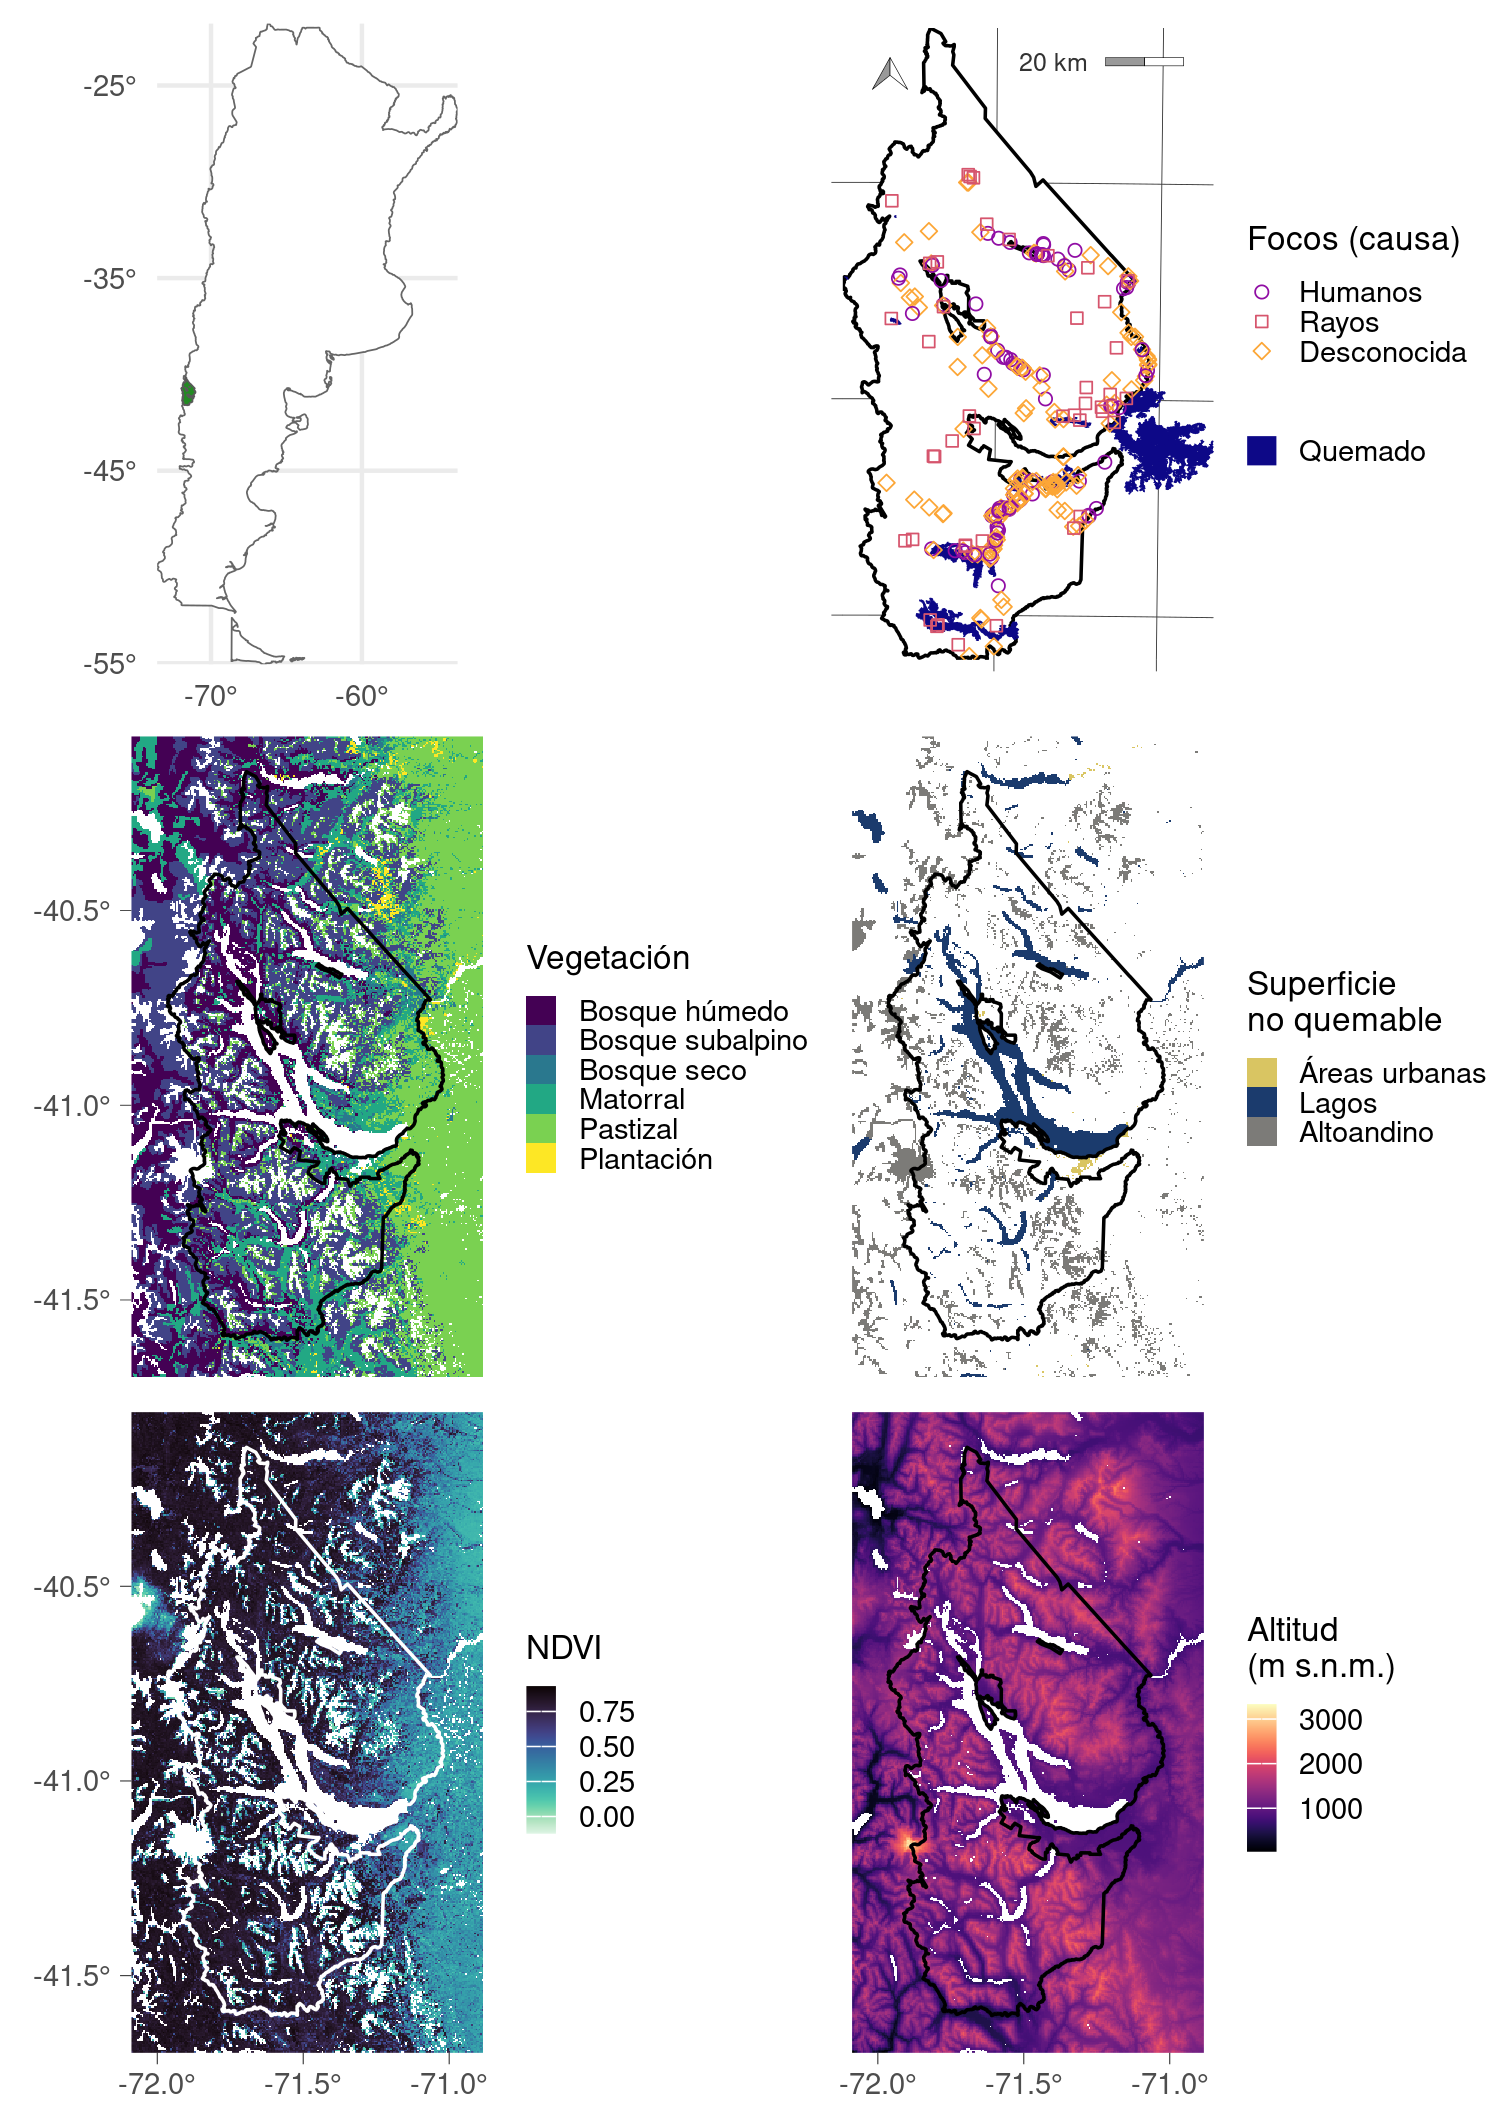
\includegraphics[width=1\textwidth]{figuras/cap4/projections/pnnh_landscape.png}
    \caption[Área de estudio, Capítulo~\ref{cap:modelos}.]{Mapas del Parque Nacional Nahuel Huapi destacando la base de datos de igniciones con el área quemada (1999-2022, mapeo del Capítulo~\ref{cap:patrones}), y algunas de las predictoras utilizadas en los modelos. Para una descripción del área de estudio, ver Sección~\ref{cap3:study-area}.} 
    \label{fig:pnnh_landscape}
\end{figure}

\subsection{Representación de los efectos de la vegetación y la topografía}

Considerar los efectos del tipo de vegetación, la productividad y la topografía sobre la inflamabilidad requería de muchos parámetros (ver Capítulo~\ref{cap:patrones}), cuya estimación presentaba un gran desafío con la información disponible. Para reducir el número de parámetros resumimos las predictoras mencionadas con dos índices: Índice de Inflamabilidad de la Vegetación (IIV), e Índice de Inflamabilidad por Topografía (IIT). En ecología es frecuente el uso de índices para resumir numerosas predictoras, y generalmente se obtienen mediante un ordenamiento de los datos según las variables a resumir (e.g., Análisis de Componentes Principales). En este caso, el enfoque fue similar, pero en vez de un ordenamiento, utilizamos los términos del predictor lineal de una regresión logística que define la probabilidad de ocurrencia de incendios a escala regional en función de las variables de interés. Este modelo fue una simplificación del modelo conjunto desarrollado en el Capítulo~\ref{cap:patrones} (ver Apéndice~\ref{append:FI}), y tomando la media de la distribución posterior de sus parámetros definimos los índices de la siguiente manera:  

\begin{equation}
\label{eq:FI}
\begin{aligned}
    IIV &= \{[\alpha_v + \beta_v \ (NDVI - \omega_v)] + 3.487888\} \ \frac{1}{1.225364} \\
    IIT &= [(-0.002407865 \ E + 0.2937129 \ N) + 2.691936] \ \frac{1}{0.852505} \\
    N & = \cos \left(L \  \frac{\pi}{180}\right) \ \frac{1}{1 + \exp(-5 + 35 \ P)},
\end{aligned}
\end{equation}

\noindent con $\alpha_v$, $\beta_v$ y $\omega_v$ definidos en la Tabla~\ref{tab:fi_params_veg} y variando por tipo de vegetación ($v$). $E$ es la altitud en m s.n.m., $N$ es el componente norte de la orientación de la ladera ($L$, en grados), y $P$ es la pendiente de la ladera (°). De esta manera, $N$ está ponderado por la pendiente, tomando valores cercanos a cero cuando la pendiente es baja. Ambos índices están escalados para tener media 0 y desvı́o 1 sobre el área de estudio del Capı́tulo~\ref{cap:patrones}. Las tablas~\ref{tab:IIV-values} y \ref{tab:IIT-values} muestran valores de estos índices para condiciones contrastantes de vegetación y topografía, y la figura~\ref{fig:FI} muestra cómo varı́an los ı́ndices en función de cada una de las variables que los definen.

\begin{table}[h]
    \centering
    \caption[Parámetros que definen el índice de inflamabilidad de la  vegetación.]{Parámetros que definen el índice de inflamabilidad de la  vegetación (IIV).}
    \label{tab:fi_params_veg}
    \begin{tabular}{l|c|c|c}
    \toprule
    Parámetro        & $\alpha$  & $\beta$    & $\omega$  \\
    \midrule
    Bosque húmedo    & -2.550628 & -44.552187 & 0.6624889 \\
    Bosque subalpino & -2.502559 & -52.508023 & 0.6988966 \\
    Bosque seco      & -2.707386 &  -3.716391 & 0.6537689 \\
    Matorral         & -2.603914 &  -4.409584 & 0.6669274 \\
    Pastizal         & -2.625388 & -10.730352 & 0.6233552 \\
    \bottomrule
    \end{tabular}
\end{table}

\begin{table}[h]
    \centering
    \caption[Índice de Inflamabilidad de la Vegetación en función del tipo de vegetación.]{Índice de Inflamabilidad de la Vegetación (IIV) en función del tipo de vegetación, para valores esperados de NDVI a 900 m s.n.m., en laderas con orientación este y con pendiente de 10°. El NDVI esperado fue predicho en base al modelo descripto en el Apéndice~\ref{append:spread-veg-effects}.}
    \label{tab:IIV-values}
    \begin{tabular}{l|rr}
    \toprule
    Tipo de vegetación & NDVI & IIV \\
    \hline
    Bosque húmedo & 0.823 & -0.176 \\
    Bosque subalpino & 0.817 & 0.209 \\
    Bosque seco & 0.664 & 0.637 \\
    Matorral & 0.703 & 0.717 \\
    Pastizal & 0.469 & 0.494 \\
    \bottomrule
    \end{tabular}
\end{table}

\begin{table}[h]
    \centering
    \caption[Índice de Inflamabilidad por Topografía para valores contrastantes de altitud y orientación.]{Índice de Inflamabilidad por Topografía (IIT) para valores contrastantes de altitud y orientación, fijando la pendiente en 10°.}
    \label{tab:IIT-values}
    \begin{tabular}{ccc}
    \toprule
    Altitud (m s.n.m.) & Orientación & IIT \\
    \hline
    500 & N & 1.808\\
    1000 & N & 0.396\\
    1500 & N & -1.016\\
    500 & E/O & 1.746\\
    1000 & E/O & 0.333\\
    1500 & E/O & -1.079\\
    500 & S & 1.683\\
    1000 & S & 0.270\\
    1500 & S & -1.142\\
    \bottomrule
    \end{tabular}
\end{table}

\FloatBarrier

\subsection{Definición y estimación de modelos}

\subsubsection{Modelo de ignición}

Definimos la ignición como la ocurrencia de un foco en una celda con vegetación con un tamaño y duración suficientes como para que el ICE del PNNH fuera notificado, excluyendo de la base de datos los focos en infraestructura humana. Separamos el proceso de ignición en dos submodelos: temporal y espacial (Fig.~\ref{fig:esquema}A). Por un lado, modelamos el número total de igniciones en toda el área de estudio (el PNNH) por quincena, separando igniciones humanas de aquellas causadas por rayos, y considerando como única predictora el FWI. Por otro lado, modelamos la ubicación de las igniciones como una regresión logística condicional, sorteando en qué celdas ocurrían las igniciones según variables espaciales de resolución media-alta (vegetación, topografía, e influencia humana; Fig.~\ref{fig:esquema}A). Si bien modelar directamente la probabilidad de ignición por celda y quincena sería más flexible, esto implicaría un alto costo computacional, ya que se requería calcular la probabilidad de ignición en todas las celdas del paisaje en cada quincena y simular un proceso de Bernoulli. Dado que el FWI tiene muy baja resolución espacial (24 km) comparado con las demás predictoras (30 m) y que la utilizamos como anomalía (i.e., sin patrón espacial en promedio), simulamos el número de igniciones en toda el área, utilizando el promedio espacial del FWI por quincena. De esta manera, sólo se debe sortear qué celdas se queman cuando las igniciones ocurren. Además, la regresión logística condicional permite aproximar el proceso simulando la ignición en un pequeño subconjunto de celdas seleccionadas al azar, en vez de calcular la probabilidad en todo el paisaje.

El modelo temporal de igniciones para el PNNH se define así:

\begin{equation}
\label{eq:igrate}
\begin{aligned}
    N_{tc} &\sim \text{Binomial Negativa}(\lambda_{tc}, \phi_{tc}) \\
    \lambda_{tc} &= \frac{\upsilon_c}{1 + \exp{(-\eta_{tc})}} \ A\\
    \eta_{tc} &= \beta_{0,c} + \beta_{1,c} \ x_t \\
    x_t &= \sum_{l=0}^{10} FWI_{t-l} \ \frac{w_l}{\sum_{j=0}^{10} w_j}\\
    w_l &= e^{-\left(\frac{l}{\tau}\right)^2}\\
    \phi_{tc} &= \gamma_{0c} + \gamma_{1c} \ \lambda_{tc} \\ 
    \\
    \upsilon_c &\sim \text{Normal}(14/A, 14/A)\text{T}[0, ] \\ 
    \beta_{0c} &\sim \text{Normal}(0, 10) \\
    \beta_{1c} &\sim \text{Normal}(0, 5)\text{T}[0, ] \\
    \gamma_{0c} &\sim \text{Normal}(0, 50)\text{T}[0, ] \\
    \gamma_{1c} &\sim \text{Normal}(0, 10)\text{T}[0, ] \\
    \tau &\sim \text{Normal}(0, 8.25)\text{T}[0, ]. 
\end{aligned}
\end{equation}
\addcontentsline{equations}{subsection}{\ref{eq:igrate} Modelo de tasa de ignición.}

\noindent $N_{tc}$ es el número de igniciones de la quincena $t$ con causa $c \in \{\text{humanos, rayos}\}$ en todo el PNNH. La distribución Binomial Negativa se parametriza con media ($\lambda$) y precisión ($\phi$), con $\text{Var}(N) = \lambda + \lambda^2 / \phi$. $\upsilon$ es el máximo que puede alcanzar la tasa de ignición por quincena y por $\text{km}^2$. En la definición de la media ($\lambda$) se incluye el factor $A$ (el área del PNNH, $7161.577\ \text{km}^2$), para escalarla al número de igniciones esperado para todo el parque. $x$ es un promedio ponderado del FWI desde la quincena focal ($t$) hasta 10 quincenas atrás ($t-10$), con los pesos decayendo de forma exponencial cuadrática hacia el pasado. La rapidez de este decaimiento es controlada por el parámetro $\tau$. La distribución Normal es parametrizada con media y desvío, con $\text{T}[0, ]$ indicando si la distribución fue truncada ([límite inferior, límite superior]), donde la omisión de un límite indica $\pm\infty$. Modelamos $\lambda$ con una función logística para evitar que las predicciones tomaran valores extremadamente altos al predecir valores fuera del rango observado de $x$. Con el mismo espíritu, definimos $\phi$ como una función lineal creciente de $\lambda$, evitando que el modelo simulara valores extremos de $N$, lo cual podía ocurrir incluso si $\lambda$ presentaba un límite superior.

El modelo espacial de igniciones ubica en el paisaje todas las igniciones simuladas por el modelo temporal en cada quincena, evaluando por separado igniciones humanas y por rayos. Este proceso se simula como un muestreo de celdas quemables sin reemplazo, en donde cada celda tiene una probabilidad inicial $\theta_i$, que depende de características del paisaje, de las cuales, sólo el índice de inflamabilidad de la vegetación (IIV) varía entre años, y ninguno varía entre quincenas. Estrictamente, la distribución de la identidad de las celdas quemadas por cada causa se podría describir como una hipergeométrica multivariada, en donde se ofrece sólo un elemento de cada ítem (celda; \citealt{fog2008calculation}). Sin embargo, dado que el número de celdas quemadas es notablemente menor al número de celdas quemables, la verosimilitud se puede aproximar usando la distribución categórica, tratando por separado cada ignición, lo que equivale a suponer $N_{tc} = 1$ bajo la formulación hipergeométrica:

\begin{equation}
\label{eq:igspat}
\begin{aligned}
    i_{tc} &\sim \text{Categórica}(\boldsymbol{\theta}_{tc}) \\
    \theta_{itc} &= \frac{\exp{(\eta_{itc})}}{\sum_{j=0}^{C_t} \exp{(\eta_{jtc})}} \\
    \eta_{itc} &= \beta_{1c} \ IIV_{it} + \beta_{2c} \ IIT_i + \beta_{3c} \ DP_i + \beta_{4c} \ DC_i\\
    \\
    \beta_{kc} &\sim \text{Normal}(0, 10)T[0, ] \  \text{para} \ k \in \{1, 2\} \\
    \beta_{kc} &\sim \text{Normal}(0, 10)T[, 0] \  \text{para} \ k \in \{3, 4\} \ \text{y}\  c = \text{humanos} \\
    \beta_{kc} &= 0 \  \text{para} \ k \in \{3, 4\} \ \text{y}\  c = \text{rayos}.
\end{aligned}
\end{equation}

\noindent $i_{tc} \in \{1, ..., C_t\}$ identifica cada celda quemable del PNNH en la quincena $t$, mientras que $C_t$ es el número total de celdas quemables. $\boldsymbol{\theta}$ es un vector de probabilidades de largo $C_t$ que suma 1, y se calcula a partir de los predictores lineales, $\eta_i$. $IIV$ e $IIT$ son los índices de inflamabilidad de la vegetación y por topografía, respectivamente, definidos en \eqref{eq:FI}; $DP$ y $DC$ representan la distancia al poblado y al camino más cercano, respectivamente. Nótese que los coeficientes que multiplican dichas distancias están restringidos a ser negativos en el caso de igniciones humanas (mayor distancia, menor probabilidad relativa de ignición), y son fijados en cero para las igniciones por rayos. A su vez, los coeficientes de los índices de inflamabilidad están restringidos a ser positivos (mayor inflamabilidad, mayor probabilidad relativa de ignición). Cabe remarcar que para estimar estos modelos sólo contábamos con datos de focos, sin poder separar el proceso de ocurrencia de rayos u ocurrencia de una fuente de calor generada por humanos (e.g., una brasa que vuela desde una fogata) de la subsiguiente propagación a pequeña escala que genera un foco detectable. Por este motivo, consideramos que la vegetación y la topografía pueden afectar la ocurrencia de focos, tanto naturales como antrópicos, no por determinar dónde se producen rayos o fuentes de calor antrópicas, sino por regular la propagación inicial que define si la fuente de calor se llega a convertir en un foco. 

Incluso utilizando la aproximación categórica, calcular los $\theta_{itc}$ para todas las celdas del paisaje es altamente costoso, tanto para realizar simulaciones como para ajustar el modelo. Por lo tanto, utilizamos una segunda aproximación. Para estimar el modelo representamos el conjunto de celdas quemables del paisaje con una muestra al azar de 10000 celdas. Como la única predictora que varía en el tiempo es el IIV, este se calcula para todos los años en que tenemos datos (focos) para esas 10000 celdas. De esta manera, al ajustar el modelo calculamos únicamente 10000 $\times$ años valores de $\eta_i$ para cada causa (los coeficientes varían entre causa humana o por rayos). Así, los $\theta_{itc}$ asociados a cada ignición observada se calculan sobre una muestra compuesta por la celda en donde se observó la ignición y las 10000 celdas potenciales. Para simular el proceso, tomamos una muestra de 2000 celdas para cada causa, a modo de reducir aún más el costo computacional, ya que las simulaciones requieren repetir esto en cada quincena. 

El modelo fue estimado con enfoque bayesiano, usando Stan para muestrear la distribución posterior de los parámetros \citep{stan_development_team_rstan_2022}. Corrimos 8 cadenas markovianas de Monte Carlo, por 2500 iteraciones cada una, dejando 1500 para \textit{warm-up}. El muestreo convergió ($\hat{R}_{\text{max}} = 1.002096$) y se obtuvo un número efectivo de muestras suficiente (mínimo = $2478.018$).

\subsubsection{Modelo de escape}

Dado que una gran proporción de focos no llega a extenderse por más de una celda de 30 m, definimos como escape al hecho de que un foco propagara fuera de la celda en que se originó \citep{marchal_turning_2020}. El modelo de escape es una regresión logística que determina la probabilidad de que el fuego escape de la celda en que se inició (Fig.~\ref{fig:esquema}B). Entre las predictoras se incluyen la vegetación, la topografía, la influencia humana y el tiempo atmosférico, y los parámetros no varían entre igniciones causadas por humanos o por rayos:

\begin{equation}
\label{eq:escape}
\begin{aligned}
    y_{it} &\sim \text{Bernoulli}(\theta_{it}) \\
    \theta_{itc} &= \frac{1}{1 + \exp{(-\eta_{it})}} \\
    \eta_{it} &= \beta_0 + \beta_1 \ IIV_{it} + \beta_2 \ IIT_i + \beta_3 \ DP_i + \beta_4 \ DC_i + \beta_5 \ x_{it} \\
    x_{it} &= \sum_{l=0}^{10} FWI_{i,t-l} \ \frac{w_l}{\sum_{j=0}^{10} w_j} \\
    w_l &= e^{-\left(\frac{l}{\tau}\right)^2}\\
    \
    \\
    \beta_0 &\sim \text{Normal}(0, 3) \\ 
    \beta_k &\sim \text{Normal}(0, 5)\text{T}[0, ] \  \text{para} \ k \in \{1, 2, 5\} \\
    \beta_k &\sim \text{Normal}(0, 5) \  \text{para} \ k \in \{3, 4\} \\
    \tau &\sim \text{Normal}(0, 8.25)\text{T}[0, ]. 
\end{aligned}
\end{equation}

\noindent $y_{it} \in \{0, 1\}$ indica si la ignición ocurrida en la celda $i$ en la quincena $t$ propagó fuego a sus vecinas. Nuevamente, el IIV varía entre años, por lo que en todas las quincenas del mismo año toma el mismo valor. El efecto de dicha variable, así como los efectos del IIT y del FWI fueron restringidos a tomar valores positivos. 

El modelo fue estimado con enfoque bayesiano, usando Stan \citep{stan_development_team_rstan_2022}. Corrimos 8 cadenas markovianas de Monte Carlo, por 2500 iteraciones cada una, dejando 1500 para \textit{warm-up}. El muestreo convergió ($\hat{R}_{\text{max}} = 1.0032$) y se obtuvo un número efectivo de muestras suficiente (mínimo = $1998.468$).

\subsubsection{Modelo de propagación}\label{cap4:spread-model}

El modelo de propagación simula el contagio del fuego desde celdas encendidas a sus 8 vecinas, con una estructura muy similar al propuesto por Morales et al. (\citealt{morales_stochastic_2015}; Fig.~\ref{fig:esquema}C). Si bien la simulación es un proceso iterativo, se asume que los incendios transcurren enteramente en una quincena, es decir, el modelo es atemporal dentro de ese período. Las celdas tienen tres estados posibles: encendida, quemable, y no quemable. Las celdas encendidas sólo pueden mantenerse así durante una iteración (paso de ahora en más), luego de la cual se vuelven no quemables (quemadas). Algunas celdas pueden ser no quemables desde el comienzo, como aquellas ubicadas sobre cuerpos de agua o zonas no vegetadas, o quemadas en una quincena previa en el mismo año. La simulación comienza con al menos una celda quemada, y en cada paso, se simula la propagación desde cada celda encendida a sus vecinas quemables como un proceso Bernoulli. El paso se completa una vez que se simuló propagación desde todas las celdas encendidas. La probabilidad de propagación se define como una función logística de las variables ambientales. Los términos de esta función corresponden al IIV e IIT de la celda receptora y a efectos direccionales del viento y la pendiente, los cuales se calculan a partir de variables correspondientes a las celdas dadora y receptora. Se asume que la distancia a caminos y poblados no afectan la probabilidad de propagación. Las celdas receptoras con más de una vecina encendida pueden recibir fuego de todas ellas; es decir, si la primera vecina no la quema, puede ser quemada por la segunda, y así sucesivamente hasta completar la revisión de sus vecinas encendidas (máximo 8). En ese proceso, el orden en que se simula la propagación desde sus vecinas es indistinto. La simulación termina cuando se alcanza el máximo número de pasos, pero puede terminar antes si, por azar, ninguna celda encendida logra propagar fuego a sus vecinas. 
La propagación $y \in \{0, 1\}$ desde la celda $i$ hacia una celda vecina quemable $j$ en el paso $k$ se define de la siguiente manera:

\begin{equation}
\label{eq:datamodel}
\begin{aligned}
    y_{ijk} &\sim \ \text{Bernoulli}(\theta_{ijk}) \\
    \theta_{ijk} &= \frac{\mathbb{I}_{k \le \kappa}}{1 + \exp{(-\eta_{ij})}} \\
    \eta_{it} &= \beta_0 + \beta_1 \ IIV_j + \beta_2 \ IIT_j + \beta_3 \ S_{ij} + \beta_4 \ W_{ij} \\
    S_{ij} &= \sin\left[ \tan^{-1} \left( \frac{E_j - E_i}{G_{ij}} \right) \right] \, \mathbb{I}_{E_j - E_i > 0}, \\
    W_{ij} &= \cos(A_{ij} - D_i) \ V_i
\end{aligned}
\end{equation}

\noindent $\theta$ es la probabilidad de propagación, y $\mathbb{I}_{k \le \kappa}$ es una variable indicadora que toma 1 si el número de pasos, $\kappa$, no ha sido superado, y 0 en caso contrario. $S_{ij}$ y $W_{ij}$ son términos que representan los efectos direccionales de la pendiente y el viento, respectivamente. $E$ es la altitud sobre el nivel del mar de cada celda (m), $G_{ij}$ es la distancia (m) entre celdas, $A_{ij}$ es la dirección desde donde llegaría el fuego, es decir, la posición de la celda dadora vista desde la receptora (radianes), $D_i$ es la dirección desde donde sopla el viento en la celda dadora (radianes), y $V_i$ es la velocidad del viento en la celda dadora (m/s). El primer factor en $S_{ij}$ es el seno de la pendiente entre las celdas, de tal forma que toma 1 si la celda receptora se encuentra exactamente arriba de la dadora, -1 si está exactamente debajo, y 0 si están a la misma altitud. Pero como las celdas no se solapan, su valor no suele superar $0.7101 = \sin{(45\ \text{°})}$. La variable indicadora $\mathbb{I}_{E_j - E_i > 0}$ anula este término en caso de que la propagación ocurra cuesta abajo. El primer factor en $W_{ij}$ toma 1 cuando el viento sopla en la misma dirección y sentido que la propagación, -1 si sopla en la misma dirección pero sentido opuesto, y 0 si sopla perpendicular a la dirección de las celdas dadora y receptora. La velocidad $V_i$ le da magnitud a este término. Dado que el vecindario está conformado por las 8 celdas vecinas de la celda dadora, las distancias entre celdas $G_{ij}$ y las direcciones $A_{ij}$ (en ángulos) pueden representarse mediante los siguientes esquemas:

\[
    G =
    \begin{bmatrix}
        30 \ \sqrt{2} & 30 & 30 \ \sqrt{2} \\
        30 & \cdot & 30 \\
        30 \ \sqrt{2} & 30 & 30 \ \sqrt{2}
    \end{bmatrix}, \quad
    A =
    \begin{bmatrix}
        135 & 180 & 225 \\
        90 & \cdot & 270 \\
        45 & 0 & 315
    \end{bmatrix},
\]

\noindent donde $\cdot$ representa la posición de la celda dadora, y 30 m es el tamaño de las celdas. Finalmente, los parámetros $\beta$ y $\kappa$ son cantidades desconocidas, y deben ser estimados. De ahora en más, los denominaremos conjuntamente como el vector $\boldsymbol{\beta}$:

\begin{equation}\label{eq:spread_params}
    \boldsymbol{\beta} = \{\beta_1, \beta_2, \beta_3, \beta_4, \beta_5, \kappa\}.
\end{equation}

Uno de nuestros principales objetivos era modelar los efectos de las condiciones atmosféricas sobre la propagación. Sin embargo, en la región hay una densidad muy baja de estaciones meteorológicas como para obtener datos con adecuada resolución espacial y temporal en grandes extensiones y para muchos años. Por lo tanto, obtuvimos el FWI de \citet{vitolo_era5-based_2020}, que se basa en el reanálisis climático del ERA5 \citep{hersbach2020era5}, con resolución temporal diaria y espacial de aproximadamente 24 km (0.25°). A partir de los datos diarios estandarizados a nivel de píxel, calculamos los promedios por quincena, y luego utilizamos su valor acumulado, como un promedio ponderado de la quincena focal y las anteriores, tal como en los modelos de ignición y escape. Con una resolución espacial gruesa para el FWI y con una baja variabilidad espacial (debido a la estandarización), optamos por asumir que el clima es constante en cada incendio, tomando su valor interpolado en la celda de ignición. De esta manera, incluimos el efecto de la meteorología en el modelo, modelando los parámetros de propagación ($\boldsymbol{\beta}$) como una función del FWI estandarizado, promediado y acumulado por quincena. Pero aún incluyendo esta variación, el modelo seguía siendo una representación demasiado simple de la propagación del fuego, en gran parte porque, a falta de datos, se asume que la dirección y velocidad regional del viento son constantes durante toda la simulación y no se consideran los efectos del combate del fuego en la propagación. Por lo tanto, para representar mejor la variabilidad de proceso no contemplada en el modelo especificamos un modelo estadístico para los parámetros, es decir, le dimos estructura jerárquica (i.e., modelo mixto o multinivel). Esto significa que el FWI no define de forma determinística los parámetros de propagación, sino que define la media de una distribución de parámetros. De esta manera, incendios con el mismo valor de FWI pueden presentar distintos parámetros. Esta estrategia de modelado permite representar variabilidad entre incendios en muchas variables no contempladas por el modelo (meteorología, combate del fuego, particularidades del terreno como humedad del suelo, etc.). El modelo de parámetros (para $\boldsymbol{\beta}$) fue definido de la siguiente manera:

\begin{equation}
\label{eq:hier1}
\begin{aligned}
    \boldsymbol{\beta}_{ft} &= \textbf{L} + \frac{\textbf{U} - \textbf{L}}{1 + \exp{(\boldsymbol{\eta}_{ft}})} \\
    \boldsymbol{\eta}_{ft} &\sim \ \text{Normal Multivariada}(\boldsymbol{\mu}_{ft}, \boldsymbol{\Sigma}) \\
    \boldsymbol{\mu}_{ft} &= \boldsymbol{\gamma}_0 + \boldsymbol{\gamma}_1 \ x_{ft} \\
    x_{ft} &= \sum_{l=0}^{10} FWI_{f,t-l} \ \frac{w_l}{\sum_{j=0}^{10} w_j} \\
    w_l &= e^{-\left(\frac{l}{\tau}\right)^2},
\end{aligned}
\end{equation}

\noindent donde $\boldsymbol{\beta}_{ft}$ es el vector de parámetros asociado al fuego $f$, ocurrido en la quincena $t$. $\textbf{L}$ y $\textbf{U}$ son los vectores con los límites inferiores y superiores, respectivamente, para cada parámetro que conforma el vector $\boldsymbol{\beta}_{ft}$. Restringir los parámetros permitió simplificar el proceso de estimación y facilitó aplicar restricciones de signo. De esta manera, los $\boldsymbol{\beta}_{ft}$ siguen una distribución Logit-Normal Multivariada, escalada entre $\textbf{L}$ y $\textbf{U}$. La Normal Multivariada está parametrizada por su vector de medias $\boldsymbol{\mu}$ y la matriz de varianza-covarianza $\boldsymbol{\Sigma}$. Para simplificar la estimación, el parámetro $\tau$ fue obtenido de un modelo de tamaño de incendios en función del FWI acumulado ($x$), y fijado en el modo de la posterior conjunta: $2.82$. Los límites de los parámetros fueron definidos de la siguiente manera:

\begin{equation}
\label{eq:limits}
\begin{aligned}
    \textbf{L} &= \{-50, 0, 0, 0, 0, 2\} \\
    \textbf{U} &= \{-50, 30, 30, 158.6232, 30, \psi\} \\ 
    \psi &\sim \ \text{Uniforme}(1150, 2000), \\
\end{aligned}
\end{equation}

\noindent estimando el límite superior de los pasos de simulación ($\text{U}_6 = \psi$). El límite superior en la previa de $\psi$ se fijó en 2000 porque eso implica que el fuego puede recorrer como máximo 60 km ($2000 \ \text{pasos} \times 30 \ \text{m} = 60000 \ \text{m}$), lo cual abarca la extensión oeste-este de los bosques andino-patagónicos en Argentina. Si bien podrían ocurrir incendios más grandes, se escaparían de nuestra área de estudio, y carecemos de datos para informar la probabilidad de propagación en la estepa. El límite inferior de $\psi$ se definió como el máximo valor que presentaba buen ajuste para los incendios utilizados en la estimación. 

La predictora $x$ fue estandarizada previo a la estimación, y utilicé las siguientes previas para los coeficientes de la regresión de la media ($\boldsymbol{\mu}$, en escala logit):

\begin{equation}
\begin{aligned}
    \gamma_{0p} &\sim 
    \begin{cases} 
        \text{Normal}(0, 10), & \text{para } p \in \{1, \ldots, 5\}, \\
        \text{Normal}(-3.80, 10), & \text{para } p = 6.
    \end{cases} \\
    \boldsymbol{\gamma_{1}} &\sim \ \text{Normal}(0, 10),
\end{aligned}
\end{equation}

\noindent donde el subíndice $p \in \{1, ..., 6\}$ identifica los hiperparámetros asociados a cada parámetros de propagación ($\boldsymbol{\beta}$).
 
La matriz $\boldsymbol{\Sigma}$ fue descompuesta en un vector de desvíos estándar ($\boldsymbol{\sigma}$) y una matriz de correlación ($\boldsymbol{\Omega}$) para asignarle una previa más flexible: 

\begin{equation}
\label{eq:hier2}
\begin{aligned}
    \boldsymbol{\Sigma} &= \text{diag}(\boldsymbol{\sigma}) \ \boldsymbol{\Omega} \ \text{diag}(\boldsymbol{\sigma}) \\
    \sigma_p^2 &\sim \ \text{Gama Inversa}(\alpha = 1, \beta = 0.001) \\
    \boldsymbol{\Omega} &= \text{diag}(\boldsymbol{V})^{-\frac{1}{2}} \, \boldsymbol{V} \, \text{diag}(\boldsymbol{V})^{-\frac{1}{2}}  \\
    \boldsymbol{V} &\sim \ \text{Wishart Inversa}(\nu = 7, \boldsymbol{\Sigma} = \boldsymbol{I}).    
\end{aligned}
\end{equation}

\noindent La matriz de varianza-covarianza $\boldsymbol{V}$ es una variable accesoria, utilizada únicamente para asignarle una previa Wishart Inversa a la matriz de correlación, sin que los parámetros de dicha previa afecten a los desvíos estándar ($\boldsymbol{\sigma}$). Los parámetros de la Wishart-Inversa generan una distribución aproximadamente uniforme entre -1 y 1 para los coeficientes de correlación. La densidad de la distribución Gama Inversa se define como $f(x) = \alpha^\beta/\Gamma(\beta) x^{(-1-\beta)} e^{(-\alpha/x)}$. $\boldsymbol{I}$ representa la matriz identidad.

Dado que modelamos una distribución de probabilidad (la Normal Multivariada) para los parámetros de propagación ($\boldsymbol{\beta}$), los incendios ya ocurridos y con punto de ignición conocido pueden ser simulados utilizando nuevos parámetros $\boldsymbol{\beta}$ simulados a partir de dicha distribución, en base al FWI asociado a dicho incendio, o pueden ser simulados utilizando el vector $\boldsymbol{\beta}$ estimado específicamente para ese incendio. A estos dos casos les llamamos, respectivamente, \textit{parámetros simulados} y \textit{parámetros ajustados} (ver Fig.~\ref{fig:spread-ov} y \ref{fig:spread-q}). 

Para estimar la mayor parte de los parámetros de propagación utilizamos 57 incendios con punto de ignición conocido, simulando incendios con el modelo bajo las mismas condiciones (ver detalles abajo). Sin embargo, estos incendios representaban un subconjunto de mayor tamaño en relación a los 235 incendios $\ge10$ ha mapeados (\cref{cap:patrones}), lo cual habría sesgado la estimación de los parámetros que controlan el tamaño del incendio simulado, a saber, el número de pasos ($\kappa_f$, Ecuación~\ref{eq:datamodel}) y sus hiperparámetros ($\gamma_{0,6}$, $\gamma_{1, 6}$, y $\sigma_6$; ver Ecuación~\ref{eq:hier1}). Para corregir este sesgo estimamos un modelo accesorio, que relacionando los pasos estimados de 57 incendios con su tamaño permitía inferir los pasos requeridos para los 178 incendios con punto de ignición desconocido que no se podían simular: 

\begin{equation}
\begin{aligned}
    \log(a_f) &\sim \ \text{Normal}(\mu_f, \sigma_a)\text{T}[\log(10), ] \\
    \mu_f &= \alpha_0 + \alpha_1 \ \log(\kappa_f) \\
    \alpha_0 &\sim \ \text{Normal}(-1.52, 10) \\
    \alpha_1 &\sim \ \text{Normal}(0, 10), \\
\end{aligned}
\end{equation}

\noindent donde $a_f$ es el área del incendio $f$ (ha). La previa sobre $\alpha_0$ fue centrada en la media de $\log(a)$ sobre los 235 incendios para no sesgar su estimación.

Estimar el modelo de propagación presentó un desafío considerable porque no contaba con datos de propagación celda a celda ($y_{ijk}$ en Ecuación~\ref{eq:datamodel}). Es decir, en el mejor caso, se conoce el punto de ignición y el polígono final de un incendio, pero no se sabe cómo el fuego propagó celda a celda (y tampoco sería posible registrarlo, ya que el fuego avanza de forma continua en el tiempo y en el espacio). Sin datos sobre el contagio celda a celda, no podíamos evaluar la función de verosimilitud, por lo que utilizamos Computación Bayesiana Aproximada (ABC, por sus siglas en inglés; \citealt{sisson2018handbook,beaumont2010approximate}), también usado para este fin por \citet{morales_stochastic_2015}. Este enfoque se aplica en casos donde tenemos un modelo capaz de simular datos pero no podemos evaluar de forma directa la función de verosimilitud. Básicamente consta en seleccionar los valores de los parámetros que simulen datos similares a los observados. En este caso, eso implica escoger valores de parámetros que simulen incendios similares a los observados, siempre utilizando los datos bajo los cuales sucedió cada incendio (variables espaciales, condiciones atmosféricas y punto de ignición). En el enfoque bayesiano tradicional, la distribución posterior de los parámetros ($\theta$), condicionada en los datos ($y$) se define como $p(\theta | y_{\text{obs}}) = p(y_{\text{obs}} | \theta) \ p(\theta) \ C$, donde $p(\theta | y_{\text{obs}})$ es la densidad posterior de los parámetros, $p(y_{\text{obs}} | \theta)$ es la verosimilitud, $p(\theta)$ es la densidad previa de los parámetros, y $C$ es una constante normalizadora que generalmente puede ignorarse al momento de la estimación. En ABC, la posterior no condiciona en los datos directamente sino en una medida de resumen de los mismos ($s_{\text{obs}}$):

$$p_{ABC}(\theta | s_{\text{obs}}) \propto \int K(||s_{\text{obs}} - s||) \ p(s | \theta) \ p(\theta) \ ds,$$

\noindent donde $s_{\text{obs}}$ es una medida de resumen de los datos observados, y $s$, de datos simulados por el modelo. $K()$ es una función que mapea de distancias a densidades o probabilidades, usualmente aumentando a menor distancia (\textit{kernel}), y $||\cdot||$ es alguna medida de distancia o disimilitud. $p(s | \theta)$ es una función de verosimilitud para la medida de resumen $s$ que no se puede evaluar, derivada de $p(y | \theta)$ y de $s = S(y)$. En casi todas las aplicaciones, la integración sobre $s$ se logra mediante simulación. 

En nuestro caso, $y_{\text{obs}}$ sería un vector binario (no observado), para cada incendio, indicando si el fuego propagó o no desde cada celda quemada a sus vecinas quemables, y $s_{\text{obs}} = S(y_{\text{obs}})$ es el conjunto de celdas quemadas por el incendio. Nuestra métrica de disimilitud es $||s_i - s_j|| = 1 - O_{ij}$, donde $O_{ij}$ es el solapamiento espacial entre el incendio observado y un incendio simulado: 

\begin{equation}
\label{eq:overlap}
O_{ij} = \frac{|A_i \cap A_j|}{|A_i \cup A_j|}.
\end{equation}

\noindent $O_{ij} \in [0, 1]$ toma 1 si los incendios son exactamente iguales y 0 si no comparten ni una celda quemada. $A$ indica el conjunto de celdas quemadas por cada incendio, de forma que el numerador es el número de celdas quemadas por ambos incendios, y el denominador, el número de celdas quemadas por al menos uno de los dos. Para obtener una densidad no normalizada a partir de esta métrica definimos un \textit{kernel} exponencial cuadrático:

\[
\begin{aligned}
    K[O_f(\boldsymbol{\beta})] &= \exp\{-[d_f(\boldsymbol{\beta}) / 0.025]^2\} \\
    d_f(\boldsymbol{\beta}) &= 1 - \text{min}\left[1, \frac{O_f(\boldsymbol{\beta})} {T_f}\right],
\end{aligned}
\]

\noindent donde $d_f(\boldsymbol{\beta})$ es una medida de disimilitud entre el incendio observado $f$ y un incendio simulado bajo el vector de parámetros $\boldsymbol{\beta}$, que controla la probabilidad de propagación según~\eqref{eq:datamodel}. $O_f(\boldsymbol{\beta})$ es su correspondiente valor de solapamiento espacial (Ecuación~\ref{eq:overlap}), y $T_f$ es un valor de solapamiento alto para el incendio $f$. Nótese que aquí las variables varían entre incendios porque definimos un modelo jerárquico, estimando un vector de parámetros $\boldsymbol{\beta}$ para cada incendio observado (Ecuación~\ref{eq:hier1}). Para definir $T_f$ exploramos el espacio de parámetros para cada incendio con un esquema estocástico que aseguraba encontrar regiones de alto solapamiento, simulando 50000 incendios con distintas combinaciones de parámetros. Posteriormente, $T_f$ fue definido como el mínimo solapamiento de los mejores 500 valores obtenidos (percentil 99 \%). Tanto para esta exploración como para muestrear la distribución posterior, los parámetros fueron restringidos entre $\boldsymbol{L}$ y $\boldsymbol{U}$ definidos en Ecuación~\ref{eq:limits}. Sin embargo, para reducir el costo computacional, variamos el máximo número de pasos de simulación ($U_6$, el límite para $\kappa$ en Ecuación~\ref{eq:datamodel}) entre incendios, de forma tal que su valor más alto permitiera simular fuegos tanto más grandes que el observado como para obtener un solapamiento de $\approx 0.05$, lo cual es un valor muy bajo que fácilmente se mejora utilizando menos pasos.

Debido al gran número de parámetros que presentaba el modelo, a la naturaleza estocástica de $K()$ y probablemente a sus abruptas variaciones en función de $\boldsymbol{\beta}$, las técnicas convencionales de muestreo, como cadenas markovianas de Monte Carlo (MCMC por sus siglas en inglés), presentaban un costo computacional prohibitivo. Resolvimos esto combinando dos estrategias poco comunes: por un lado, utilizamos el método de \citet{lunn2013fully}, que consiste en estimar modelos jerárquicos en (al menos) dos pasos. En el primer paso se estima la distribución posterior de los parámetros a nivel de datos ($\boldsymbol{\beta}_f$ en nuestro caso, Ecuación~\ref{eq:datamodel}) de forma separada para cada grupo (incendio, $f$), y luego se combinan las muestras de dichas distribuciones para estimar los hiperparámetros ($\boldsymbol{\gamma}_0$, $\boldsymbol{\gamma}_1$, $\psi$, $\boldsymbol{\sigma}$, y $\boldsymbol{\Omega}$; ver Ecuaciones~\ref{eq:hier1},~\ref{eq:limits}, y~\ref{eq:hier2}). Al separar el modelo en dos partes, pudimos tratar el paso dificultoso de estimar los $\boldsymbol{\beta}_f$ con mayor flexibilidad. El método de Lunn requiere que en el primer paso se defina una distribución previa sustituta para cada $\boldsymbol{\beta}_f$, cuya influencia es descontada en el segundo paso, al estimarse los hiperparámetros que constituyen la verdadera previa de los primeros. La segunda estrategia fue explotar la sustitución de la previa para generar una que aumentara la eficiencia de un muestreo por rechazo. Utilizamos lo que llamamos \textit{previas redundantes} para los $\boldsymbol{\beta}_f$ y distribuciones de propuestas con forma similar a $K(\boldsymbol{\beta_f})$. Estas estrategias lograron una eficiencia aceptable del muestreo por rechazo. Para definir las previas redundantes y la distribución de propuestas utilizamos las 50000 simulaciones del período de exploración del espacio de parámetros. Para cada simulación calculamos $K()$ y remuestreamos 10000 vectores de parámetros con reemplazo, con probabilidad proporcional a $K()$. Como distribución previa redundante utilizamos una Normal Multivariada ajustada a esas muestras incrementando los desvíos estándar por un factor de 5. Como distribución de propuesta utilizamos una distribución Normal Multivariada Asimétrica ajustada a las muestras. Para que estas distribuciones fueran medianamente razonables, trabajamos en el espacio de parámetros no restringido ($\boldsymbol{\eta}$, ver~\ref{eq:hier1}). En este paso utilizamos un muestreo por rechazo adaptado a simuladores costosos (ver sección 4.2.3.4 en \citep{sisson2018handbook}) hasta obtener un número efectivo de muestras $\ge 10000$. En el paso 2, corrimos un MCMC sobre todos los parámetros, pero utilizando las muestras del paso 1 como distribución de propuestas para los $\boldsymbol{\beta}_f$, descontando el efecto de las previas sustitutas (redundantes) del paso 1, y utilizando actualizaciones Gibbs para la mayor parte de los hiperparámetros \citep{lunn2013fully}.

Escribimos el simulador de incendios en \cpp con la colaboración de Iván Renison, quien lo estructuró en el paquete de R \texttt{FireSpread} (\url{http://github.com/barberaivan/FireSpread.git}), a través de \texttt{Rcpp} \citep{Rcpp}. Tanto para el modelo de propagación como para los anteriores utilizamos R 4.2.0 \citep{R}. El código se encuentra disponible en GitHub (\url{https://github.com/barberaivan/fire_spread}). Para manejar datos espaciales utilizamos el paquete \texttt{terra} \citep{terra}.

\subsubsection{Simulador del régimen de incendios}



Este modelo integra los procesos de ignición, escape y propagación, simulándolos en todas las quincenas de un año (Fig.~\ref{fig:esquema}). La capa de vegetación se fija utilizando el NDVI promedio del verano anterior para calcular el IIV. Las celdas quemadas en cada quincena no pueden ser quemadas nuevamente en las sucesivas quincenas. Para calibrar este modelo al PNNH, disminuimos el intercepto de la regresión de pasos ($\gamma_{0,6}^* = \gamma_{0,6} - 0.95$) para que la probabilidad de quema anual se asemejara a la registrada en el parque de acuerdo a los datos del Capítulo~\ref{cap:patrones} (período 1999-2022). Esta corrección fue necesaria porque el modelo de propagación fue ajustado a incendios $\ge 10$ ha, no a la distribución completa del tamaño de incendios, ya que no contábamos con suficientes datos para tal fin. 

Este modelo toma como entrada un ráster de FWI quincenal para todo un año en el PNNH, y devuelve un ráster binario indicando qué celdas se quemaron, a 30 m de resolución. Simulando este proceso por muchas iteraciones se puede obtener un mapa de probabilidad de quema anual calculando en qué fracción de los años simulados (iteraciones) se quemó cada celda del paisaje. A su vez, también se pueden calcular la proporción del área quemable del PNNH que se quema cada año y la proporción del área quemada correspondiente a igniciones por rayos.

\begin{figure}[H]
    \centering
    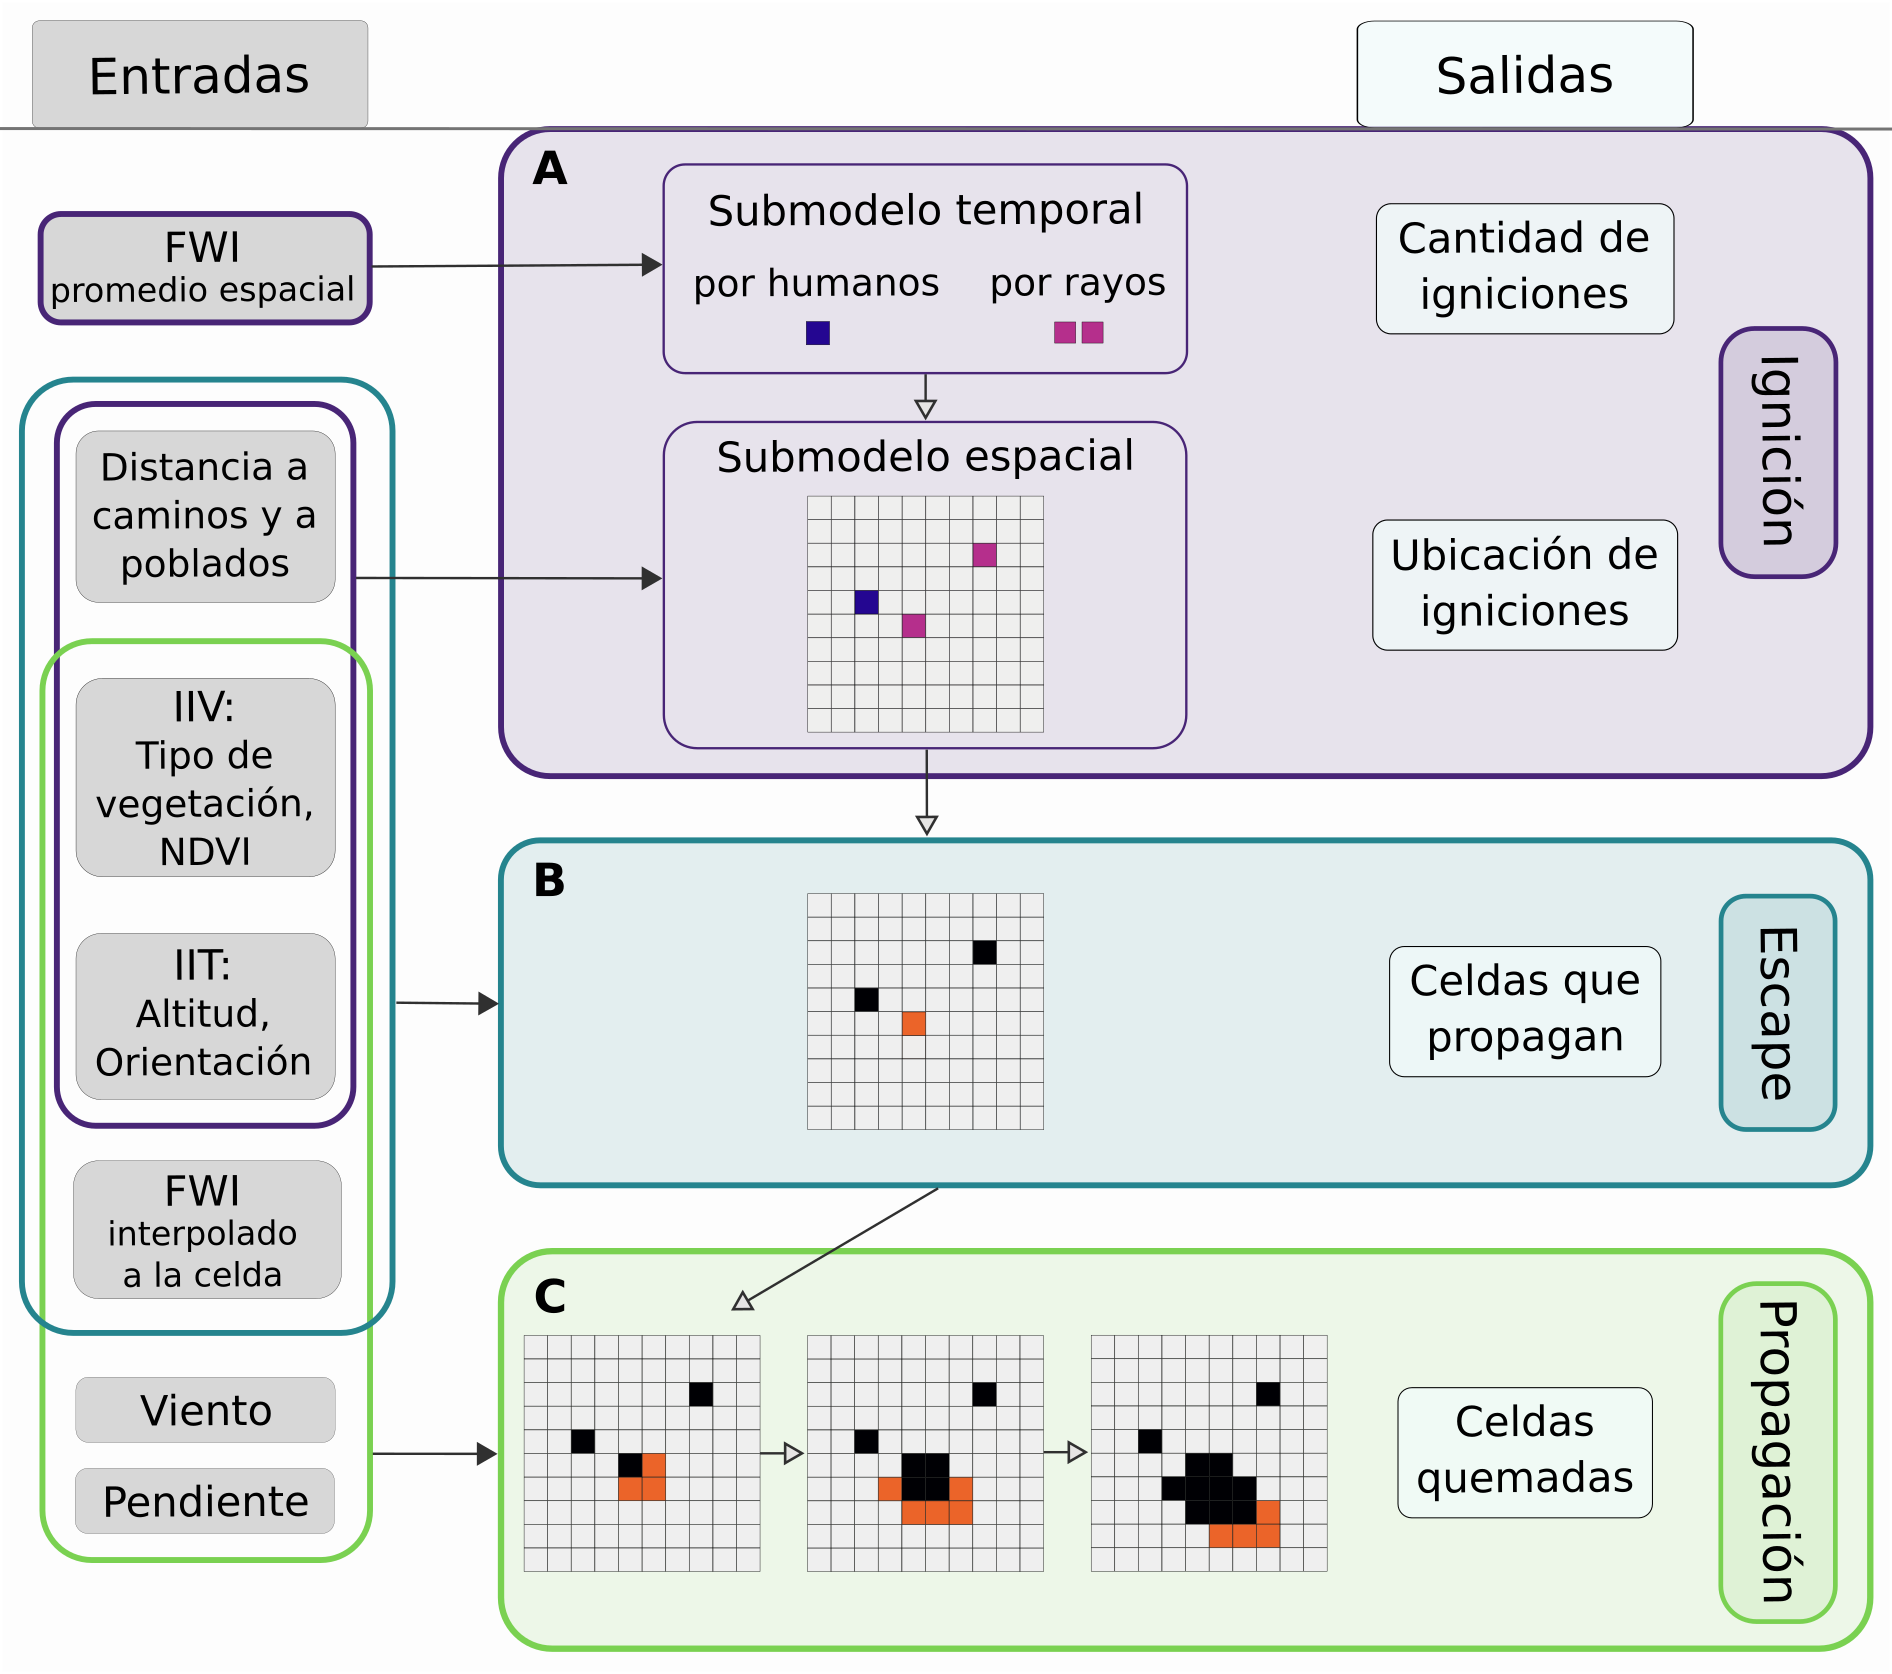
\includegraphics[width=13cm]{figuras/cap4/spread/esquema_modelos_fig2.png}
    \caption[Esquema de modelos de simulación.]{Esquema de los modelos de simulación. (A) El modelo de ignición está compuesto por dos submodelos: el temporal, que simula cuántas igniciones ocurren en toda el área de estudio por causa, en función del FWI promedio del área de estudio; y el espacial, que simula en qué celdas del paisaje ocurren dichas igniciones, en función de variables espaciales. La distancia a caminos y a poblados sólo regula la ubicación de igniciones humanas. El esquema ilustra un ejemplo con una ignición por humanos y dos por rayos. (B) El modelo de escape simula cuáles de las celdas en donde ocurrió ignición propagan fuego, sin importar su causa, en base a variables espaciales y al FWI interpolado a nivel de celda. En el esquema las celdas sin escape se representan en negro, y en naranja, una celda con escape. (C) El modelo de propagación simula el contagio desde las celdas en donde el fuego escapó, en función de variables espaciales y del FWI interpolado en cada celda. El esquema ilustra tres pasos de simulación, en donde el naranja representa las celdas encendidas en cada paso, que pasan a estar quemadas (negro) en el paso siguiente. La ignición, el escape, y la propagación se concatenan en cada quincena de simulación. Al simular el régimen de incendios, toda la rutina se repite a lo largo de todas las quincenas de un año, conformando una iteración. Dentro de una iteración, las celdas quemadas no pueden volver a quemarse. El NDVI se fija en el promedio del verano (dic-mar) en el año anterior al focal, por lo que no varía entre quincenas. El FWI varía entre quincenas pero tiene resolución espacial gruesa (24 km) comparado con las demás variables (30 m). IIV: Índice de Inflamabilidad de la Vegetación; IIT: Índice de Inflamabilidad por Topografía.}
    \label{fig:esquema}
\end{figure}


\FloatBarrier

\subsection{Proyecciones de la probabilidad de quema anual bajo escenarios de cambio climático}

Utilizando el simulador del régimen de incendios comparamos la probabilidad anual de quema en el PNNH para los períodos moderno (1998-2022) y las décadas de los 2040s (2040-2049) y 2090s (2090-2099). Para los períodos futuros utilizamos los escenarios SSP1-2.6, SSP2-4.5, SSP3-7.0 y SSP5-8.5 \citep{IPCC2023}. Estos escenarios representan trayectorias contrastantes de desarrollo socioeconómico y emisiones de gases de efecto invernadero. En el extremo más benévolo, el escenario SSP1-2.6 asume fuerte cooperación internacional, desarrollo sostenible y bajas emisiones. En el extremo más pesimista, el SSP5-8.5 representa un futuro con alta dependencia de combustibles fósiles y emisiones muy elevadas. Los escenarios intermedios (SSP2-4.5 y SSP3-7.0) reflejan trayectorias con esfuerzos de mitigación limitados o desigualdad regional acentuada. La elección de estos cuatro escenarios nos permitió capturar extremos y puntos intermedios del rango de proyecciones climáticas disponibles para el siglo XXI.

En total, simulamos el régimen de incendios bajo 9 condiciones climáticas (de ahora en más, experimentos): período moderno + 4 escenarios climáticos futuros $\times$ 2 décadas. Para calcular el IIV utilicé la capa de NDVI medio de 2021 (diciembre-marzo). Para disminuir el efecto borde simulamos las igniciones en un polígono extendido del PNNH, mediante un \textit{buffer} de 10 km (ver contornos en Fig.~\ref{fig:bp_models}E, \ref{fig:proj-2040}, y \ref{fig:proj-2090}), escalando la tasa de ignición a esa área. El área \textit{buffer} no fue tenida en cuenta a la hora de calcular la probabilidad de quema o la proporción quemada del paisaje, ya que esta presenta efecto borde.

En cada experimento caracterizamos el régimen de incendios utilizando el clima de varios años: 24 años en el período moderno y 10 años en los escenarios futuros. Para cada condición corrimos 2000 iteraciones del simulador anual, seleccionando el año al azar dentro del período de interés para extraer el raster de FWI. En los períodos futuros, para extraer el FWI del año sorteado, también seleccionamos el modelo climático y su realización. Para ello, en cada iteración sorteamos qué modelo climático usar en base a sus pesos, y una vez escogido el modelo seleccionamos al azar una de sus realizaciones. Los pesos de los modelos fueron determinados en función de su adecuación para representar el clima moderno en el PNNH (Apéndice~\ref{append:proj}). Utilizamos los modelos climáticos del CMIP6 y sus correspondientes realizaciones que presentaban proyecciones para los 4 escenarios (Tabla~\ref{tab:climtable}). Las proyecciones de FWI diarias fueron provistas por Fulden Batibeniz y Yann Quillcaille \citep{quilcaille2023FWI}. El procedimiento para calcular las anomalías de FWI quincenales a partir de proyecciones diarias se detalla en el Apéndice~\ref{append:proj}. 

Comparamos la probabilidad de quema anual simulada entre cada experimento de dos maneras. Primero, calculamos la proporción de celdas quemadas sobre el número de celdas quemables en el PNNH por iteración (año), y estimamos la proporción media a lo largo de las simulaciones por experimento. Para esto ajustamos un modelo Beta-Binomial, en donde la media y la dispersión variaron por experimento, a través del paquete \texttt{brms} \citep{brms}, utilizando las previas débilmente informativas definidas por defecto. Segundo, realizamos un mapa de probabilidad de quema anual por experimento, calculando la proporción de iteraciones en que se quemó cada celda del paisaje. Adicionalmente, evaluamos qué proporción del área quemada anual en el PNNH fue quemada por igniciones causadas por rayos. Para ello, utilizamos el conteo de celdas quemadas por rayos sobre el total de celdas quemadas (ignorando las simulaciones en donde no hubo incendios) para ajustar un modelo Beta-Binomial y así estimar la proporción por experimento.  

\section{Resultados}

\subsection{Ignición}

La tasa de ignición por quincena y km$^2$ aumentó de forma exponencial con el FWI, siendo este efecto ligeramente mayor para las igniciones por rayo que para las humanas (\cref{fig:igrate}). A su vez, las igniciones por rayo presentaron una tasa media más baja que las humanas y mayor dispersión.

\begin{figure}[htbp]
    \centering
    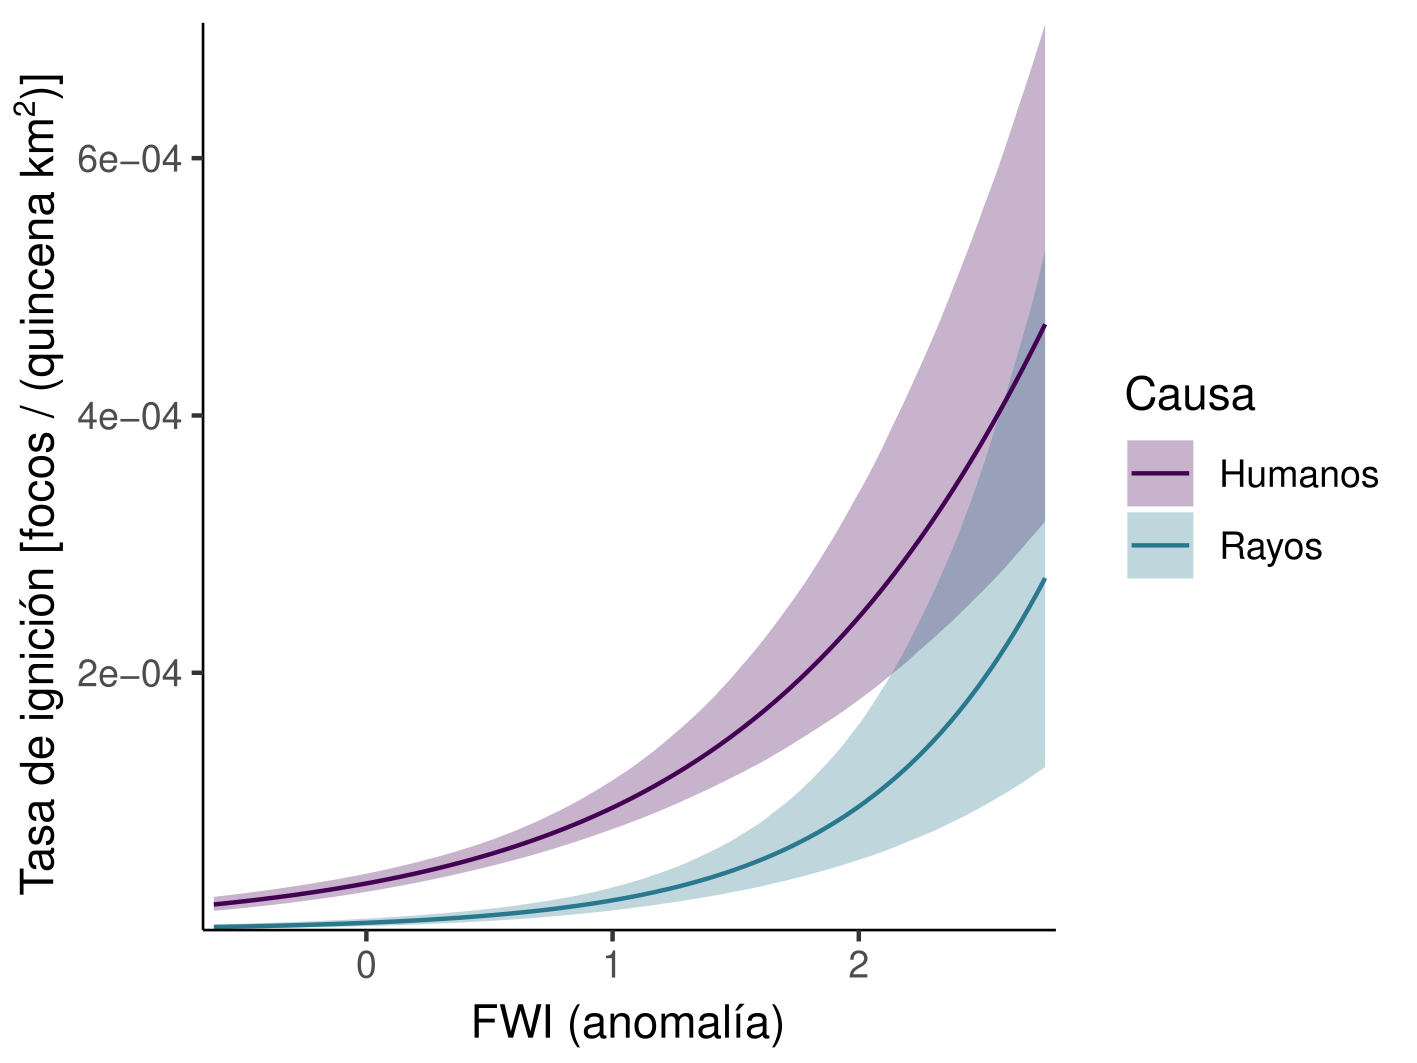
\includegraphics[width=12cm]{figuras/cap4/ignition/ignition_rate_fwi.png}
    \caption[Tasa de ignición en función del FWI.]{Tasa de ignición por quincena y km$^2$ en función de la anomalía de FWI para ambos tipos de causa. La línea y las bandas muestran la predicción de $\lambda$ (ver Ecuación~\ref{eq:igrate}), como la media y el intervalo de credibilidad del 95 \% de la distribución posterior.} 
    \label{fig:igrate}
\end{figure}

El submodelo espacial de ignición mostró un efecto considerable de la vegetación sobre la probabilidad relativa de ignición, siendo más marcado en las igniciones humanas (\cref{fig:ig_spat_veg}). De manera contraria, la topografía presentó un mayor efecto sobre las igniciones por rayos que sobre las humanas (\cref{fig:ig_spat_env}). En las igniciones humanas, las distancias a caminos y poblados presentaron efectos tan grandes que prácticamente dejaron sin efecto a las demás predictoras (Fig.~\ref{fig:ig_spat_env}, \ref{fig:bp_models}A). 

\begin{figure}[htbp]
    \centering
    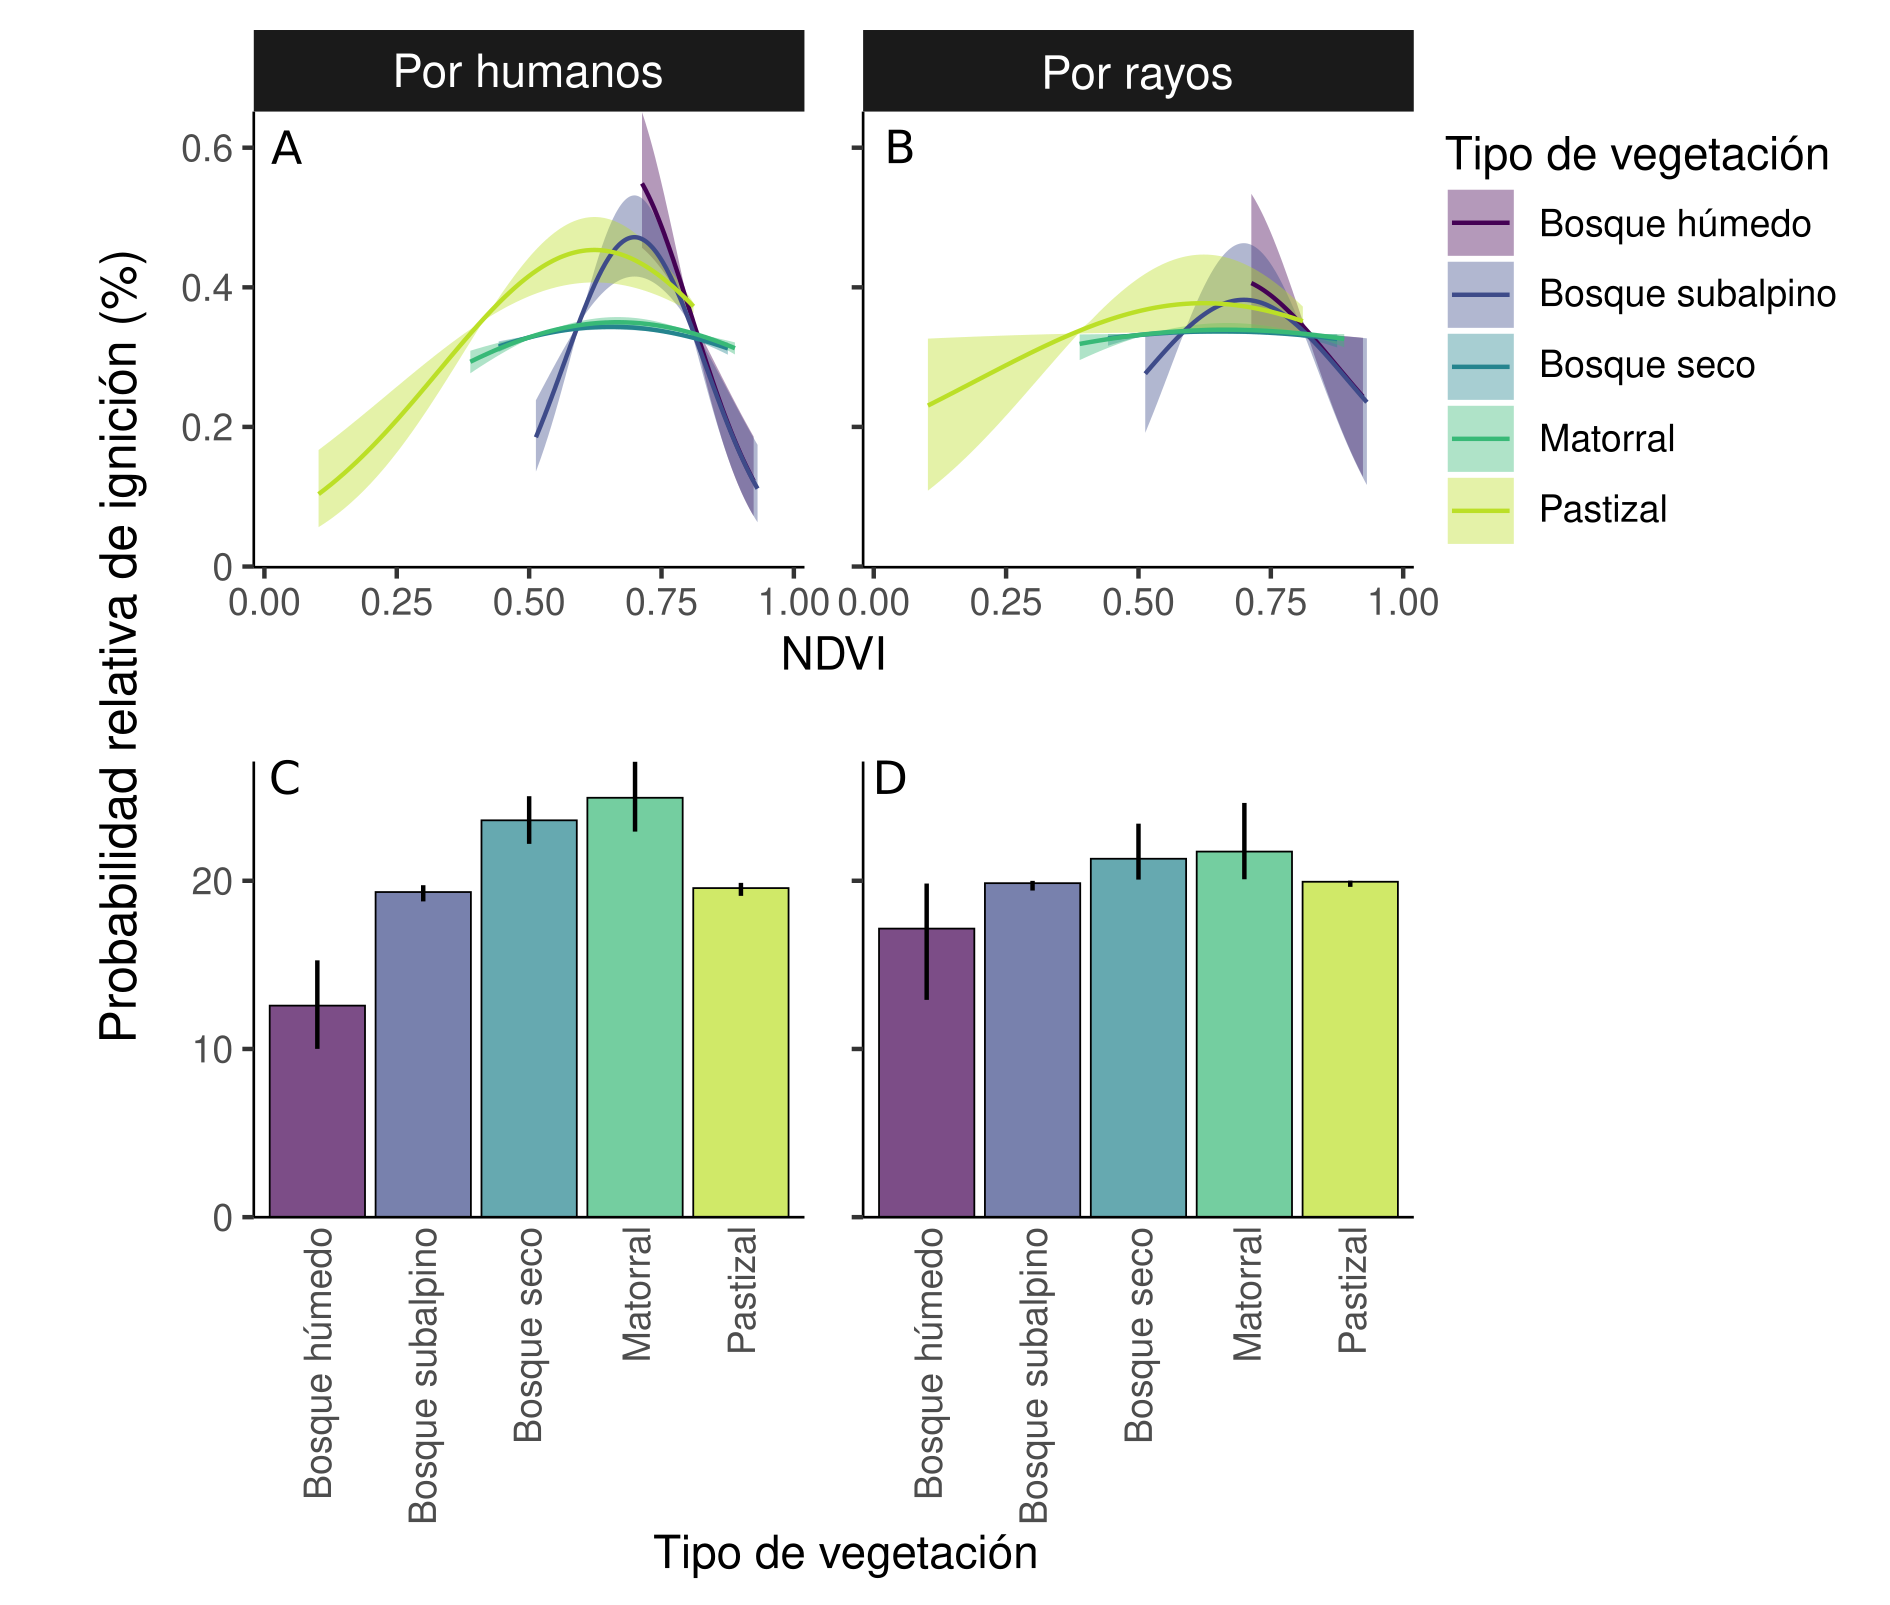
\includegraphics[width=16cm]{figuras/cap4/ignition/ignition_conditional_prob_veg.png}
    \caption[Probabilidad relativa de ignición en función de la vegetación.]{Probabilidad relativa de ignición función del NDVI por tipo de vegetación (A, B) y en función del tipo de vegetación (C, D), separando por causa, según el submodelo espacial de ignición. Las curvas fueron calculadas utilizando una secuencia regular de 300 valores de NDVI por tipo de vegetación, de forma tal que la suma de sus valores es 100 \%. Los valores de las demás predictoras fueron fijadas en sus medias. En los paneles de arriba, los valores son sólo comparables dentro de cada tipo de vegetación. Los paneles de abajo permiten comparar entre tipos de vegetación; en este caso el NDVI fue fijado en la media para cada tipo de vegetación. Las curvas (arriba) y barras (abajo) representan la media de la distribución posterior de $\theta$ (Ecuación \ref{eq:igspat}), con sus respectivos intervalos de credibilidad del 95 \% a modo de bandas o líneas verticales.} 
    \label{fig:ig_spat_veg}
\end{figure}

% Figura grande ocupando 2 páginas (figura y leyenda)
\begin{figure}[b!]
  \centering 
  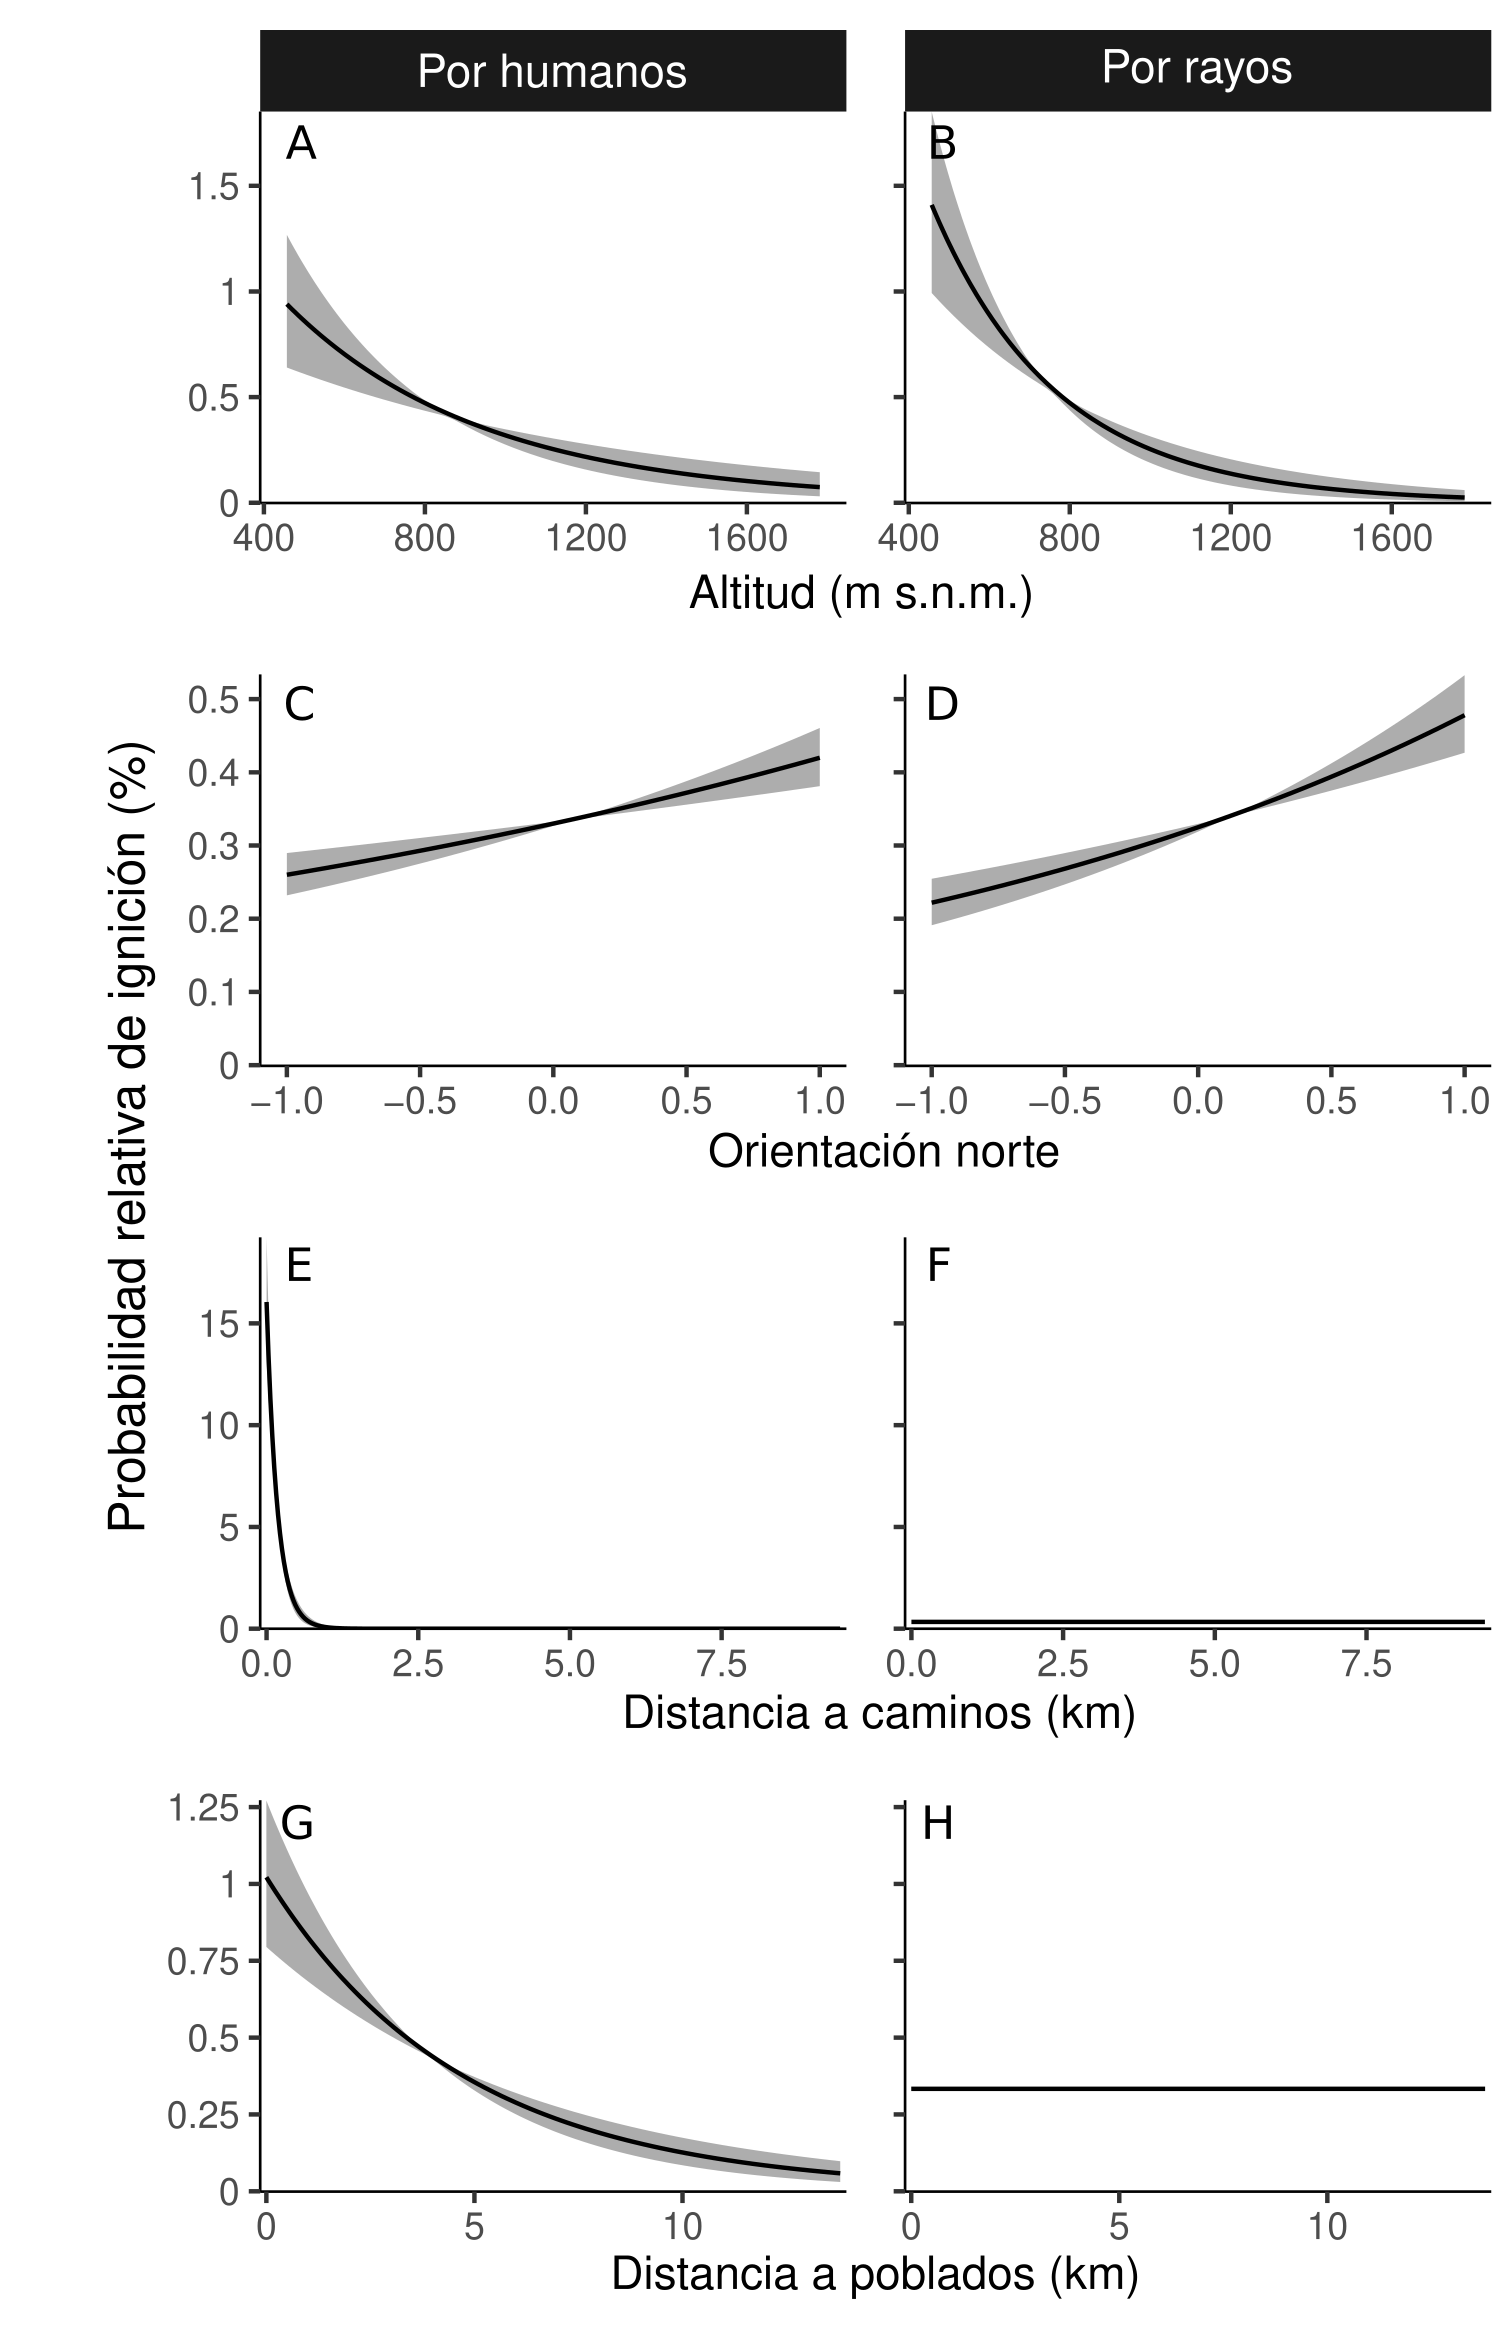
\includegraphics[width=0.8\textwidth]{figuras/cap4/ignition/ignition_conditional_prob_environment.png}
  \caption[Probabilidad relativa de ignición en función de variables ambientales.]{Probabilidad relativa de ignición en función de variables topográfias e indicadoras de influencia humana, separando por causa, según el submodelo espacial de ignición. Las curvas fueron calculadas utilizando una secuencia regular de 300 valores de cada predictora, de forma tal que la suma de sus valores es 100 \%, y las covariables no focales fueron fijadas en sus medias. Las líneas y bandas representan la media de la distribución posterior de $\theta$ (Ecuación \ref{eq:igspat}) y su intervalo de credibilidad del 95 \%, respectivamente.}
  \label{fig:ig_spat_env}
\end{figure}

\FloatBarrier % no ignition images below

\subsection{Escape}

La probabilidad de escape presentó variaciones relativamente pequeñas en función de la mayor parte de las predictoras, a excepción de las distancias a caminos y a poblados, las cuales aumentaron la probabilidad de escape (Fig.~\ref{fig:escape}). Dado que estas dos variables están correlacionadas en el paisaje (pero no en el set de datos de igniciones), su efecto conjunto puede ser considerable (Fig.~\ref{fig:bp_models}C).

% Figura grande ocupando página entera, para ubicar leyenda en la pág siguiente
\begin{figure}[b!]
  \centering 
  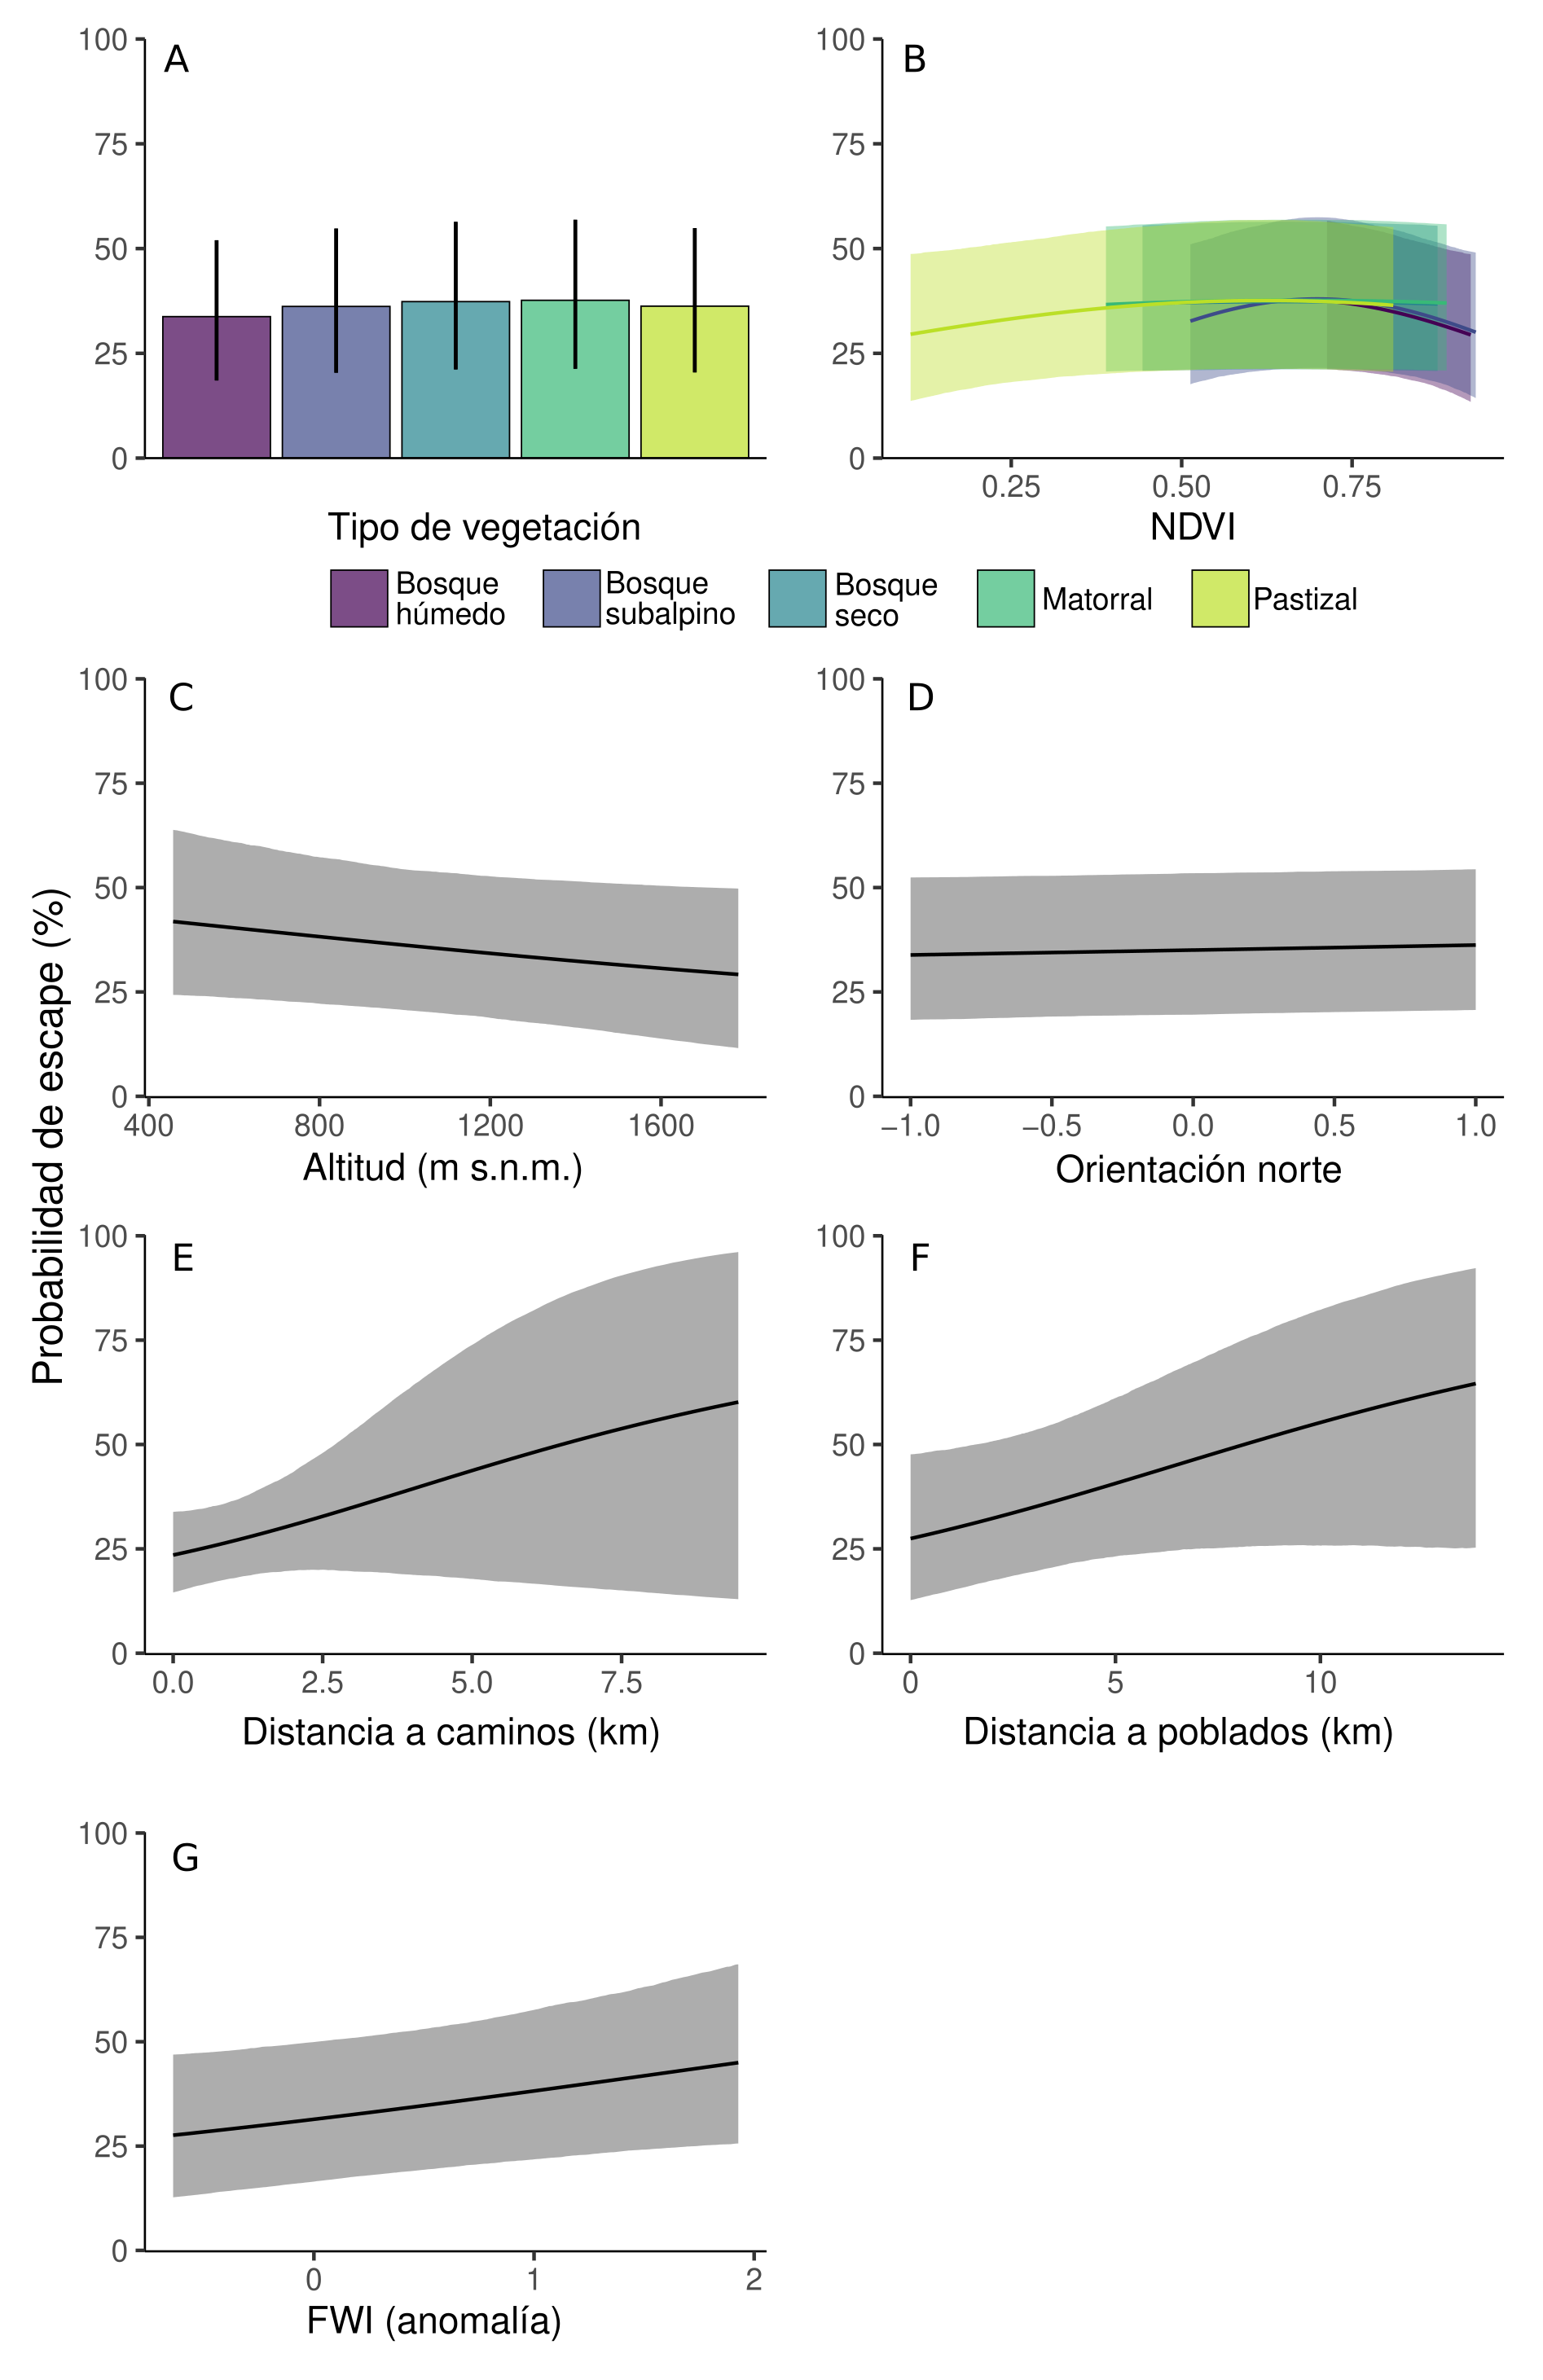
\includegraphics[height=0.95\textheight]{figuras/cap4/escape/escape_effects.png}
  \caption[Probabilidad de escape en función de las variables predictoras.]{(Leyenda en la página siguiente.)}
  \label{fig:escape}
\end{figure}

% leyenda en la página siguiente
\begin{figure}[p]
  \contcaption{(en la página anterior). Probabilidad de escape en función de las predictoras. Todas las predictoras no focales fueron fijadas en sus medias para calcular predicciones parciales. En el caso del FWI utilizamos la media acumulada en los datos de ignición (0.57). Las líneas y bandas representan la media de la distribución posterior de $\theta$ (Ecuación \ref{eq:escape}) y su intervalo de credibilidad del 95 \%, respectivamente.} 
\end{figure}

\FloatBarrier % no escape images below

\subsection{Propagación}

La probabilidad de propagación varió principalmente en función del viento y la pendiente, con los índices de inflamabilidad (vegetación y topografía) presentando efectos moderados (Fig.~\ref{fig:spread-curves} y \ref{fig:spread-curves-x}). Los parámetros de propagación presentaron una notable variabilidad no explicada entre incendios; sin embargo, algunos de ellos también variaron notablemente en función del FWI. A mayor FWI disminuyó el efecto de la pendiente y aumentó el efecto del viento (\cref{fig:spread-params}). Además de estos efectos contrapuestos del FWI sobre los efectos medios de la pendiente y el viento, el modelo estimó una correlación negativa entre estos efectos ($\beta_3$ y $\beta_4$ en la Ecuación~\ref{eq:datamodel}), reflejando que los incendios tienden a ser dominados por pendiente o por viento (\cref{fig:spread-corr}). Por otro lado, los pasos de simulación aumentaron considerablemente con el FWI, y mostraron una correlación positiva con el efecto del viento (Fig.~\ref{fig:spread-curves} y \ref{fig:spread-corr}). El efecto de la topografía (efecto no direccional de altitud y orientación; IIT) presentó un pequeño aumento en función del FWI, mientras que el efecto de la vegetación (IIV) no varió con el FWI (Fig.~\ref{fig:spread-curves} y \ref{fig:spread-veg-effects}, Apéndice~\ref{append:spread-veg-effects}).

Utilizando los parámetros estimados para cada incendio, los fuegos simulados tuvieron un solapamiento relativamente alto con los observados (\cref{fig:spread-ov}), pero este valor decreció al usar parámetros simulados desde la distribución estimada. Esto indica que la parte determinística del modelo de propagación no puede representar bien las particularidades de cada incendio, sino que gran parte de la variación se asocia a aspectos no considerados (e.g., condiciones atmosféricas a escala temporal fina, o particularidades del combate del fuego). Además, sin contar con datos de velocidad del viento para cada incendio, el modelo estima su efecto, que representa la velocidad promedio. Entonces, para poder simular fuegos similares a los ocurridos, necesitamos usar la velocidad estimada ($\beta_4$ en la Ecuación~\ref{eq:datamodel}); si simulamos velocidades a partir de la distribución estimada, los incendios simulados difieren del observado. Esto resulta esperable, ya que el viento es un factor determinante de la propagación \citep{rothermel_mathematical_1972}. El tamaño de los incendios simulados con los parámetros ajustados fue similar al tamaño observado (\cref{fig:spread-q}A), pero utilizando parámetros simulados, la discrepancia fue considerable (\cref{fig:spread-q}B). Pero a pesar de que el modelo de propagación no puede reproducir fuegos particulares salvo que se utilicen parámetros ajustados a cada incendio, el mismo puede simular incendios con una distribución de tamaño similar. Es decir, puede simular incendios con características similares a los observados. Aún así, utilizando parámetros simulados el modelo subestima la variación en tamaño de los incendios observados (nótese cómo el cociente decrece desde valores $>1$ a $<1$ en la Fig.~\ref{fig:spread-q}B).

\begin{figure}[htbp]
  \centering 
  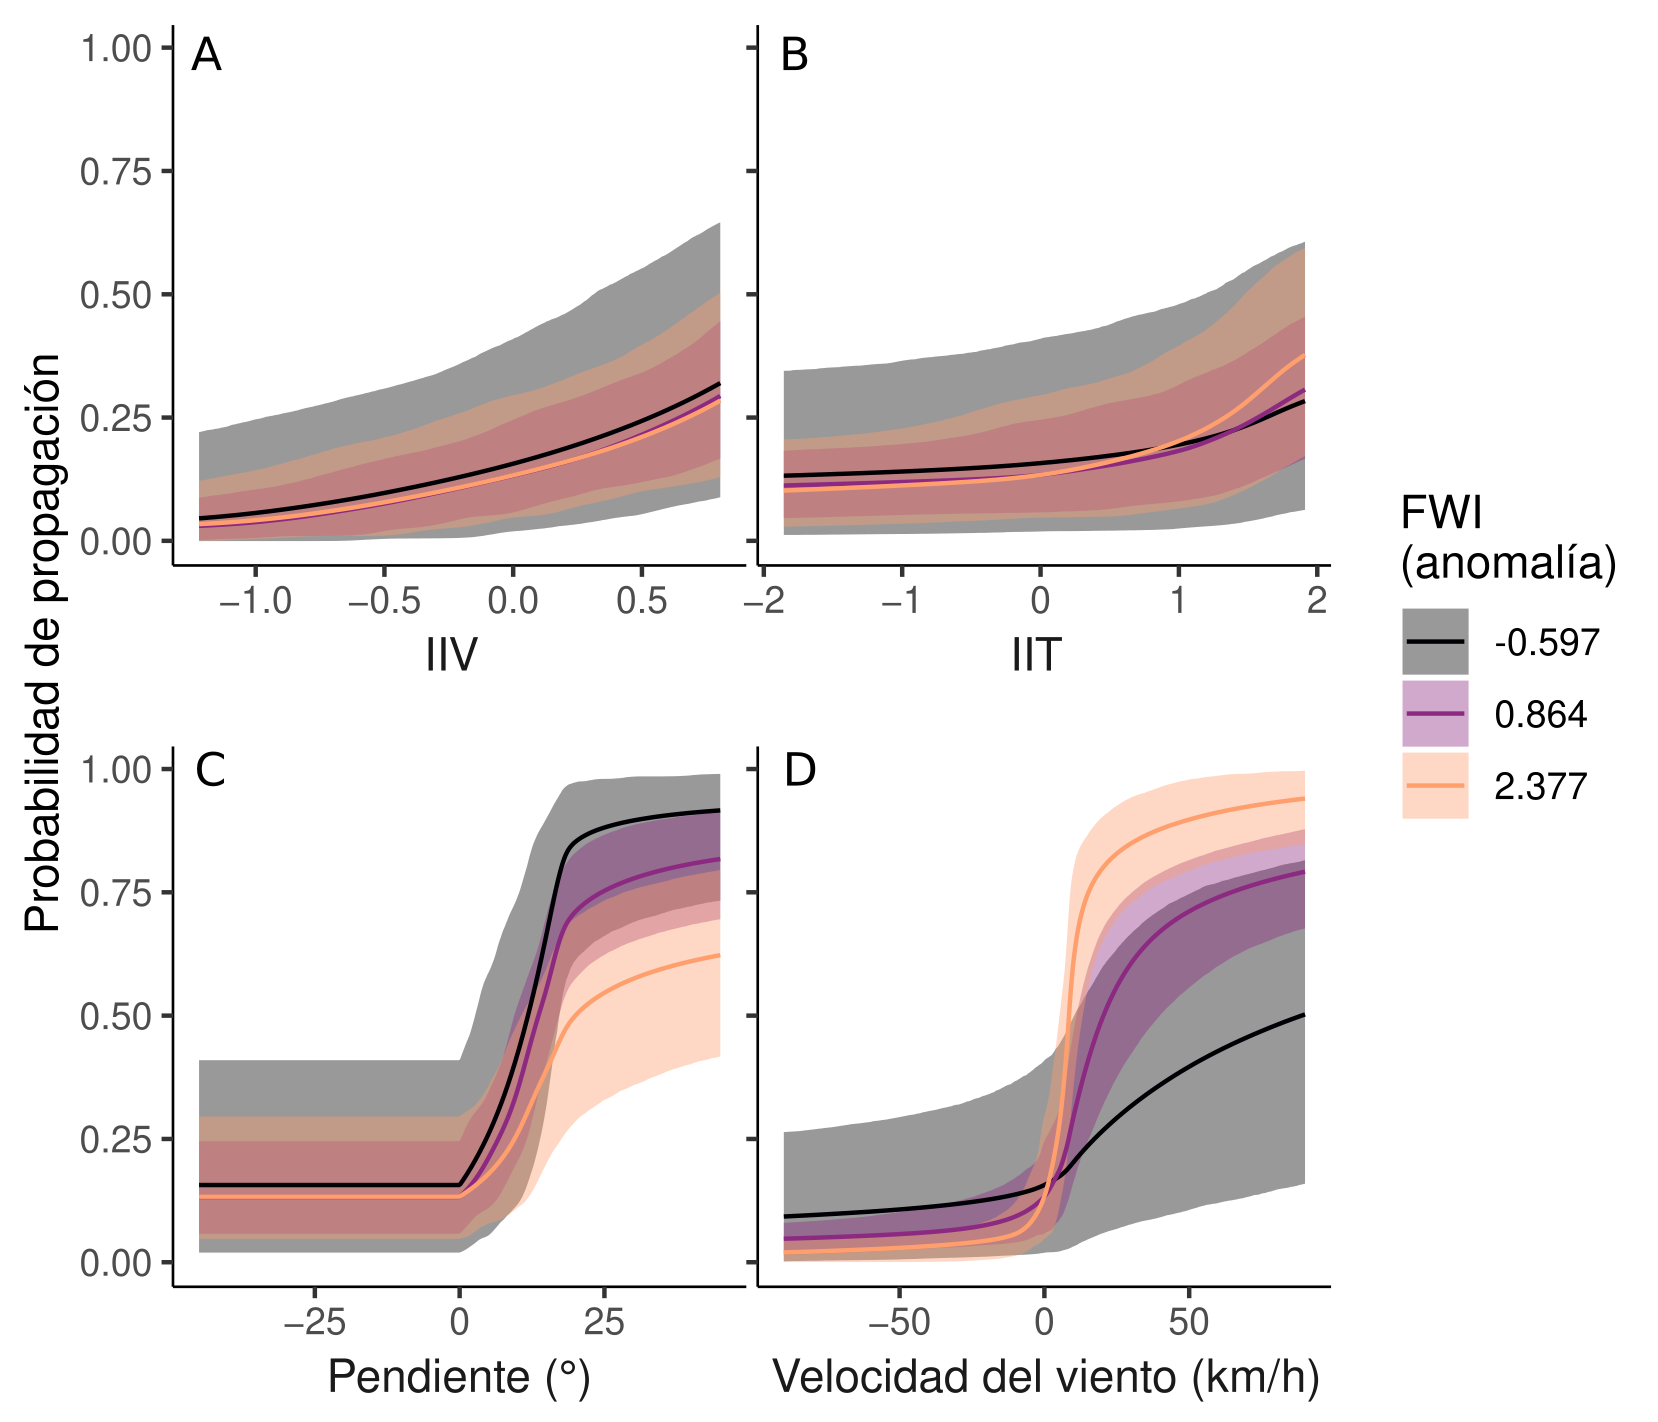
\includegraphics[width=14cm]{figuras/cap4/spread/spread_prob_curves.png}
  \caption[Probabilidad de propagación en función de la vegetación, topografía, pendiente y velocidad del viento.]{Probabilidad de propagación en función las predictoras, para tres valores contrastantes de FWI acumulado (media y percentiles 2.5 y 97.5 \% de los incendios mapeados en el Capítulo~\ref{cap:patrones}). Cada curva representa el promedio de la distribución de parámetros, calculados mediante simulación. Las líneas y bandas representan la media y el intervalo de credibilidad del 95 \% de la distribución posterior. IIV: Índice de Inflamabilidad de la Vegetación; IIT: Índice de Inflamabilidad por Topografía. Estos índices son adimensionales, y valores más altos indican mayor inflamabilidad. (Ver sus definiciones en la Ecuación~\ref{eq:FI}).}
  \label{fig:spread-curves}
\end{figure}

\begin{figure}[htbp]
  \centering 
  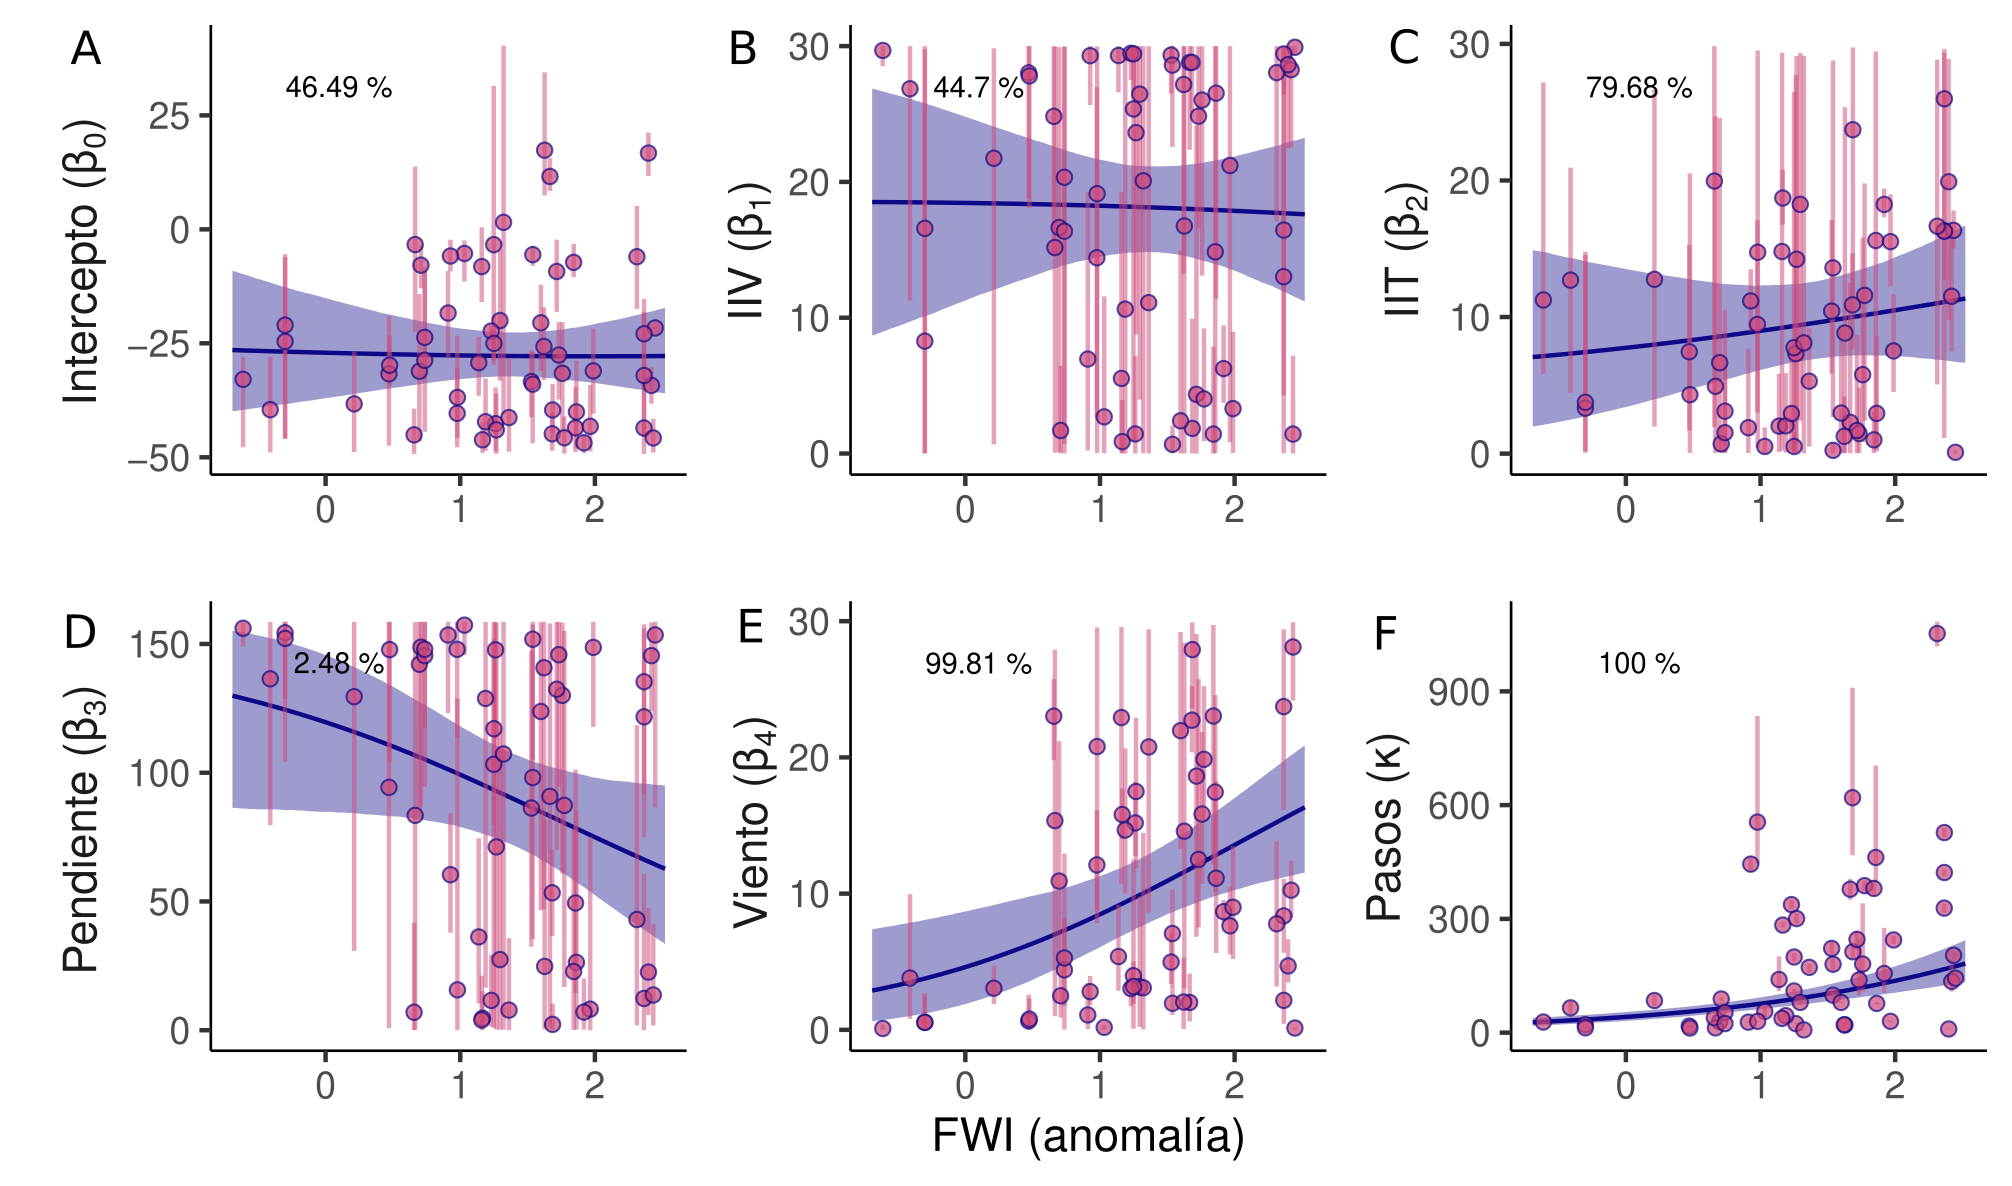
\includegraphics[width=\textwidth]{figuras/cap4/spread/params_fwi_regression.png}
  \caption[Parámetros de propagación en función del FWI.]{Parámetros de propagación en función del FWI. Las curvas y bandas muestran la media de los efectos aleatorios (como media e intervalo del 95 \% de su distribución posterior), mientas que los puntos y líneas verticales muestran el parámetro estimado para cada incendio. Los porcentajes dentro de cada panel indican la probabilidad de que la media aumente en función del FWI (0 \% indica completa certeza sobre un efecto negativo; 50 \% indica incertidumbre total sobre el signo del efecto, y 100 \% indica certeza completa de un efecto positivo). Los pasos ($\kappa$) indican el número máximo de pasos de simulación (ver Ecuación~\ref{eq:datamodel}).}
  \label{fig:spread-params}
\end{figure}

\begin{figure}[htbp]
  \centering 
  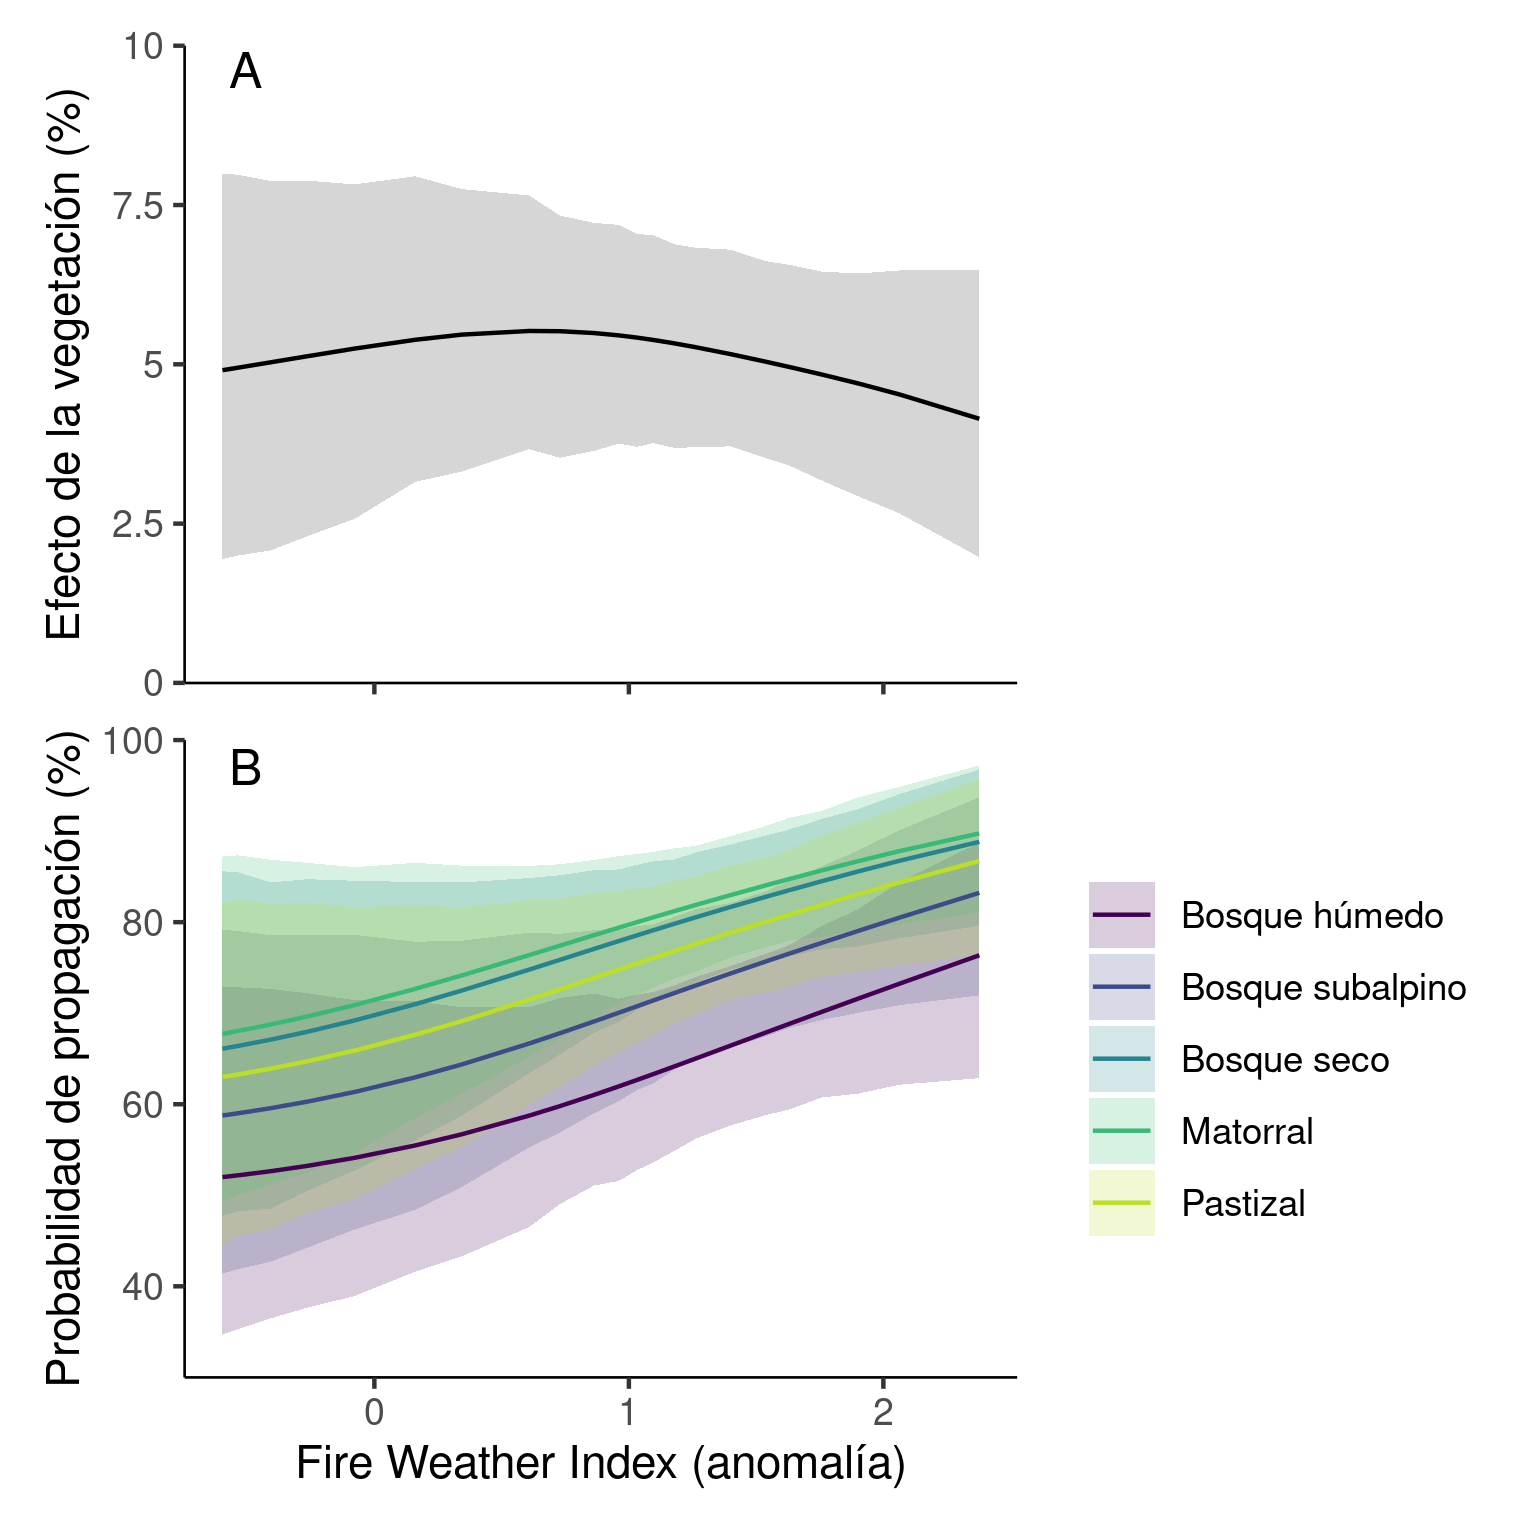
\includegraphics[width=13cm]{figuras/cap4/spread/vegetation_effects_fwi.png}
  \caption[Efecto de la vegetación sobre la probabilidad de propagación en función del FWI.]{(A) Efecto del tipo de vegetación sobre la probabilidad de propagación en función del FWI, calculado como el desvío absoluto medio entre las probabilidades estimadas para los cinco tipos de vegetación, mostradas en (B). (B) Probabilidad de propagación en función del FWI por tipo de vegetación. Para comparar la probabilidad de propagación entre tipos de vegetación, fijamos la altitud en 900 m s.n.m., la orientación en 90° (componente norte = 0), y marginalizamos sobre la distribución de NDVI, pendiente y velocidad del viento en el PNNH (detalles en el Apéndice~\ref{append:spread-veg-effects}).}
  \label{fig:spread-veg-effects}
\end{figure}

% agrandar márgenes de página
\newgeometry{top=0.5cm, bottom=0.5cm, left=1cm, right=1cm}

% Figura grande ocupando página entera, para ubicar leyenda en la pág siguiente
\begin{figure}[b!]
  \centering 
  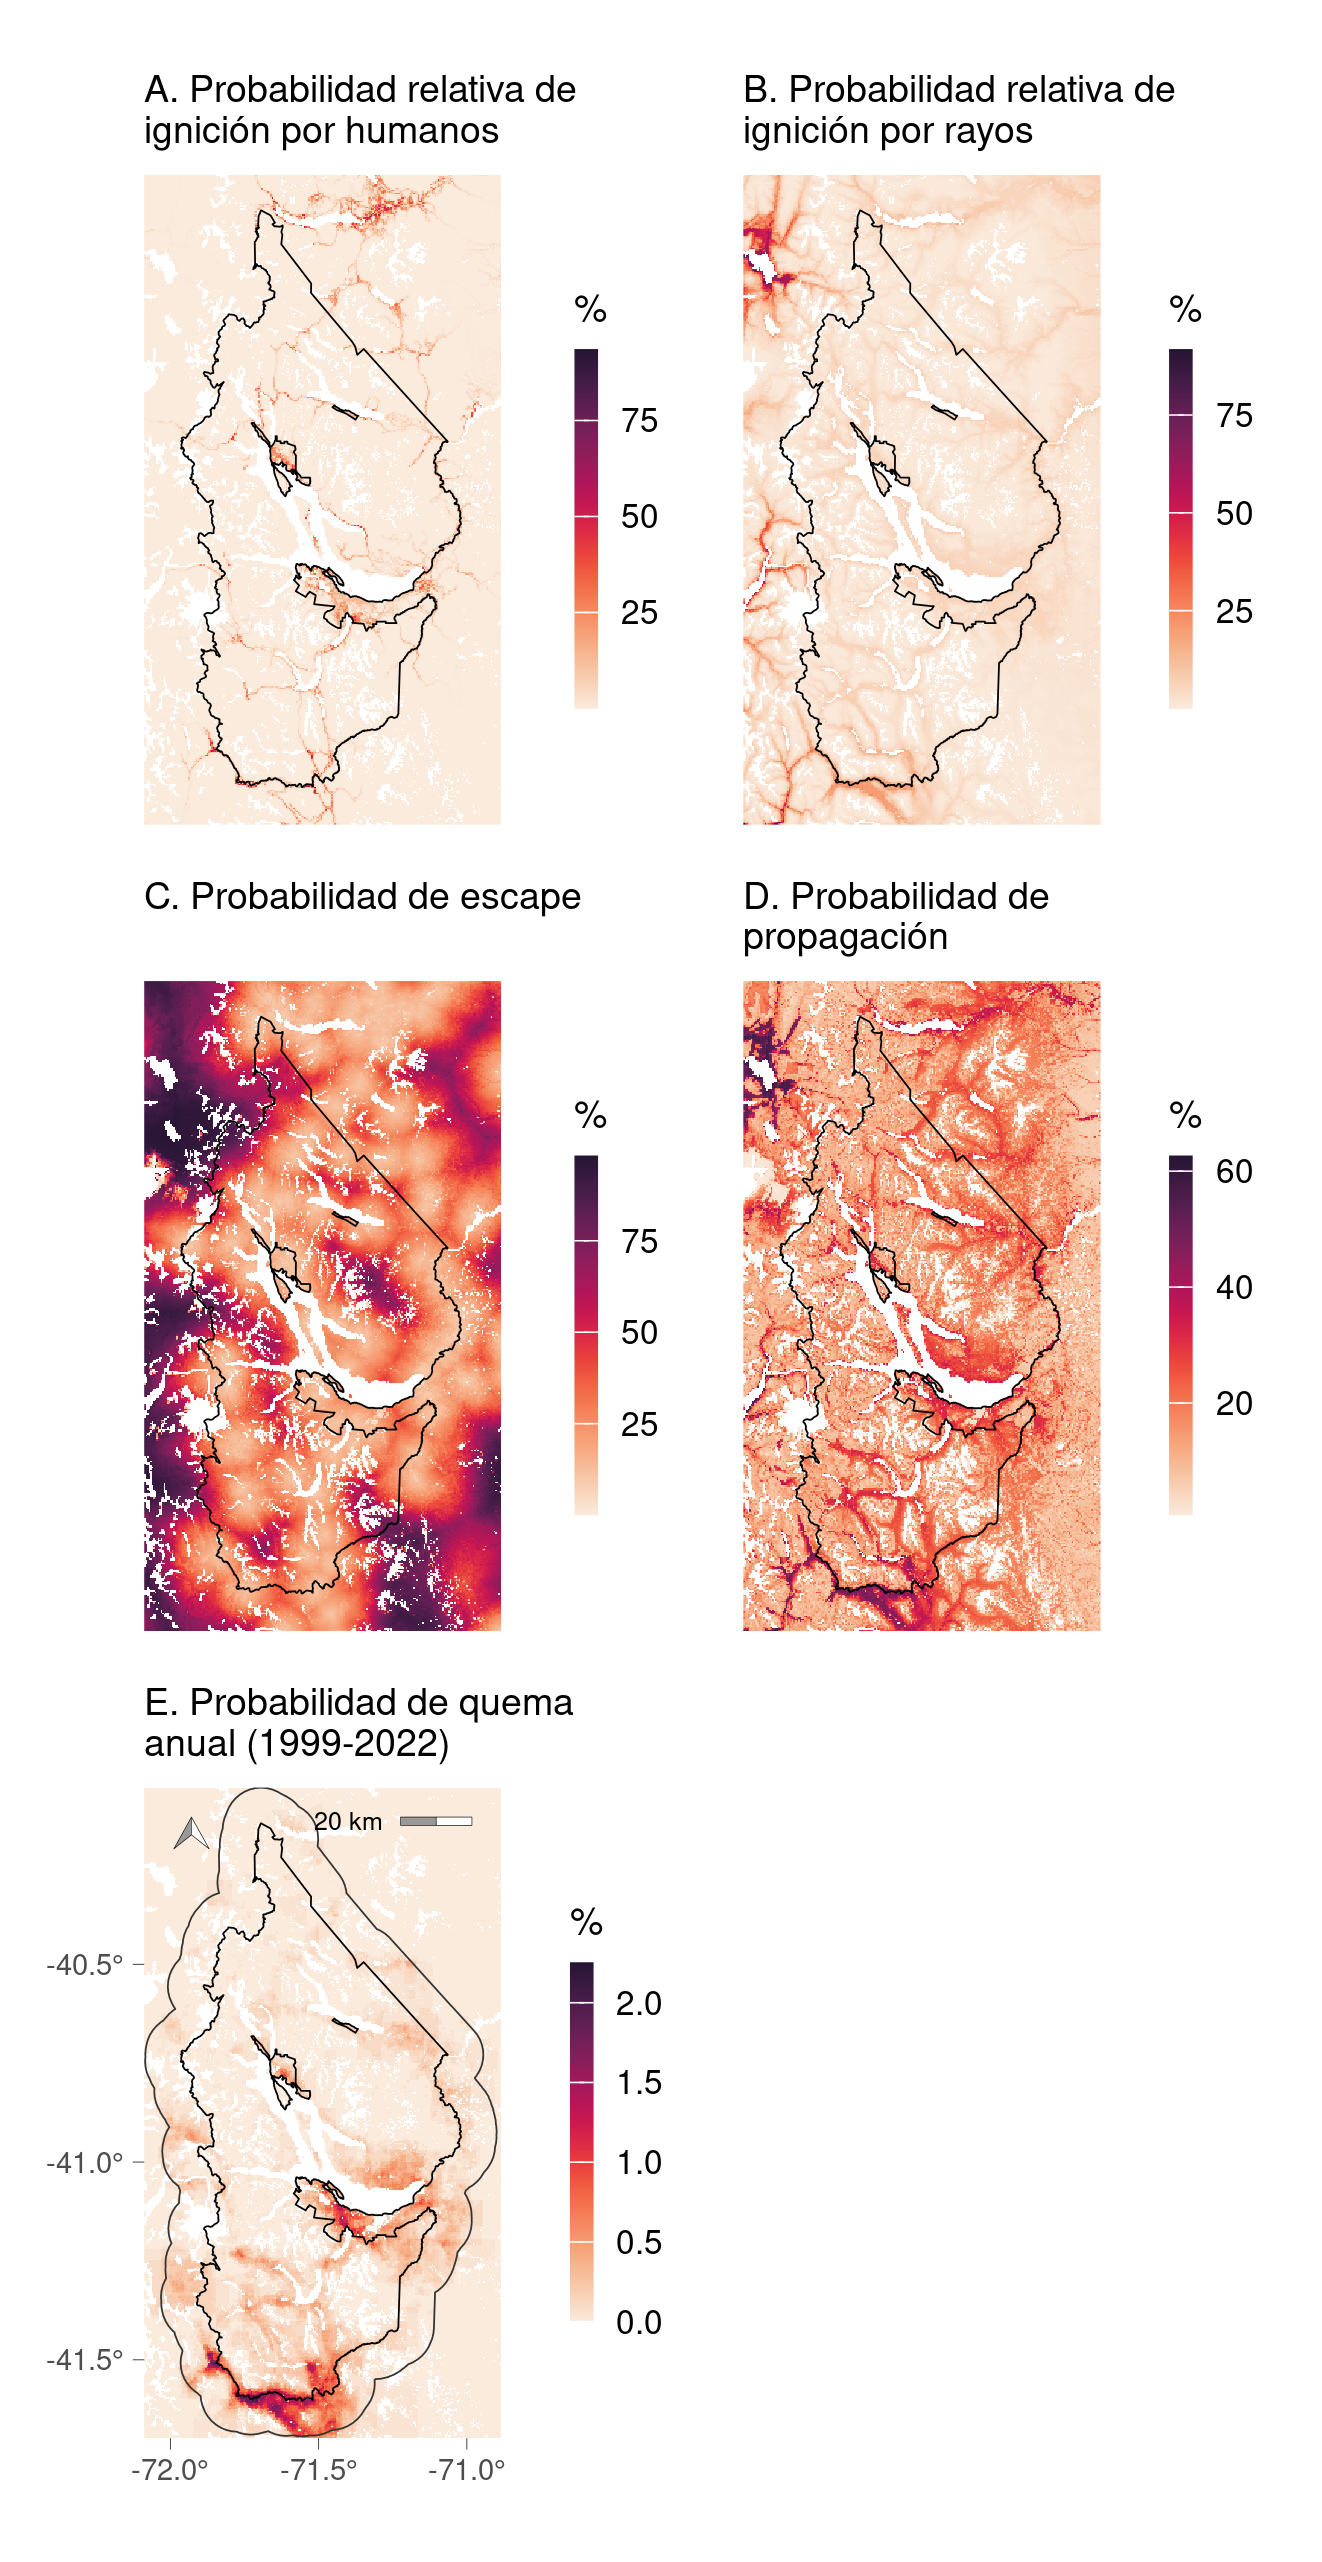
\includegraphics[width=13.8cm]{figuras/cap4/projections/burn_prob_models_modern.png}
  \caption[Probabilidad de ignición, escape, propagación y quema en el PNNH.]{(Leyenda en la página siguiente.)}
  \label{fig:bp_models}
\end{figure}

% restaurar márgenes de página
\restoregeometry


% leyenda en la página siguiente
\begin{figure}[p]
  \contcaption{(en la página anterior). Probabilidad de ignición, escape, propagación y quema en el PNNH. Las probabilidades de ignición (A, B), escape (C) y propagación (D) son predicciones de sus respectivos modelos, tomando el promedio de la distribución posterior, y fueron calculadas fijando el FWI en el promedio de la base de datos de focos. Para calcular la probabilidad de propagación se fijó la velocidad del viento en 14.4 km/h. La probabilidad de quema anual (E) se obtuvo simulando el régimen de incendios por 2000 iteraciones, integrando los tres modelos. El contorno alrededor del parque señala el área donde se simularon las igniciones, para evitar subestimar la probabilidad de quema en los bordes del PNNH.} 
\end{figure}

\FloatBarrier % no spread images below

\subsection{Proyecciones de la probabilidad de quema anual bajo escenarios de cambio climático}

La proporción quemada anual en el PNNH presentó una notable variación entre períodos y escenarios climáticos (Fig.~\ref{fig:proj-means}A, Tabla~\ref{tab:burn-prob-means}). Para los 2040s se espera que la proporción aumente en un factor de entre $\approx$ 2 y $\approx$ 2.6 con respecto al período 1999-2022, alcanzando valores entre el 0.2 y el 0.25 \% anual, según el escenario. Nótese que este valor es el mismo que encontramos para 1999-2022 en una región más amplia (Sección~\ref{cap3:patrones-regimen}), que incluye zonas con mayor incidencia del fuego que el PNNH. Para los 2090s se esperan aumentos mucho mayores en general y mucho más variables entre escenarios, con la proporción quemada anual variando entre 0.13 y 2.97 \%, lo cual representa aumentos en factores de entre 1.36 y 31.17 para los escenarios más optimista y pesimista, respectivamente (SSP1-2.6 vs. SSP5-8.5). En ambos períodos futuros y bajo todos los escenarios climáticos se espera que la proporción quemada anual media aumente, y únicamente para el escenario SSP1-2.6 en 2090-2099 se espera un aumento menor al doble con respecto al período 1999-2022 (Fig.~\ref{fig:proj-means}, Tabla~\ref{tab:burn-prob-means}). 

Más allá de las diferencias en proporción quemada anual media entre experimentos, cabe destacar que la proporción quemada varió notablemente entre años simulados, y a su vez, distintos experimentos presentaron contrastante variabilidad (Fig.~\ref{fig:proj-cdf}). Los percentiles del 95 \% de la distribución de proporción quemada anual variaron entre 0.45 \% para 1999-2022 y 14.47 \% para 2090-2099 bajo SSP5-8.5, y los máximos, entre 8.08 \% y 60.29 \%, respectivamente. 

La proporción quemada por rayos sobre el total quemado anualmente en el PNNH presentó variaciones mucho menores que la proporción quemada del paisaje, presentando aumentos marcados únicamente para el período 2090-2099 en los escenarios más pesimistas (SSP3-7.0 y SSP5-8.5, Fig.~\ref{fig:proj-means}B, Tabla~\ref{tab:burn-prob-means}). Bajo esas condiciones, se esperaría que la contribución relativa de los rayos al área quemada aumente al $\approx$ 34 \%, comparado con el $\approx$ 25 \% estimado para 1999-2022. 

Si bien la proporción quemada anual varió notablemente entre escenarios, la probabilidad de quema anual a nivel de píxel mantuvo un patrón espacial similar entre experimentos (Fig.~\ref{fig:bp_models}E, \ref{fig:proj-2040}, y \ref{fig:proj-2090}). Esto indica que la mayor incidencia del fuego no afectaría cualitativamente la disposición espacial de zonas con mayor y menor incidencia de fuego. La zona de mayor probabilidad de quema fue el valle del Manso Inferior, al sur del PNNH, debido a su baja altitud ($\approx$ 400 m s.n.m.) y a la presencia de caminos y poblados. Otras zonas de alta probabilidad de quema son los alrededores de Bariloche y Dina Huapi, que también presentan altitud relativamente baja y presencia humana. Más allá de estas zonas, se evidenció un notable efecto de la altitud, con los valles más extensos y profundos mostrando una relativamente alta probabilidad de quema luego de las zonas arriba mencionadas.

\begin{figure}[htbp]
  \centering 
  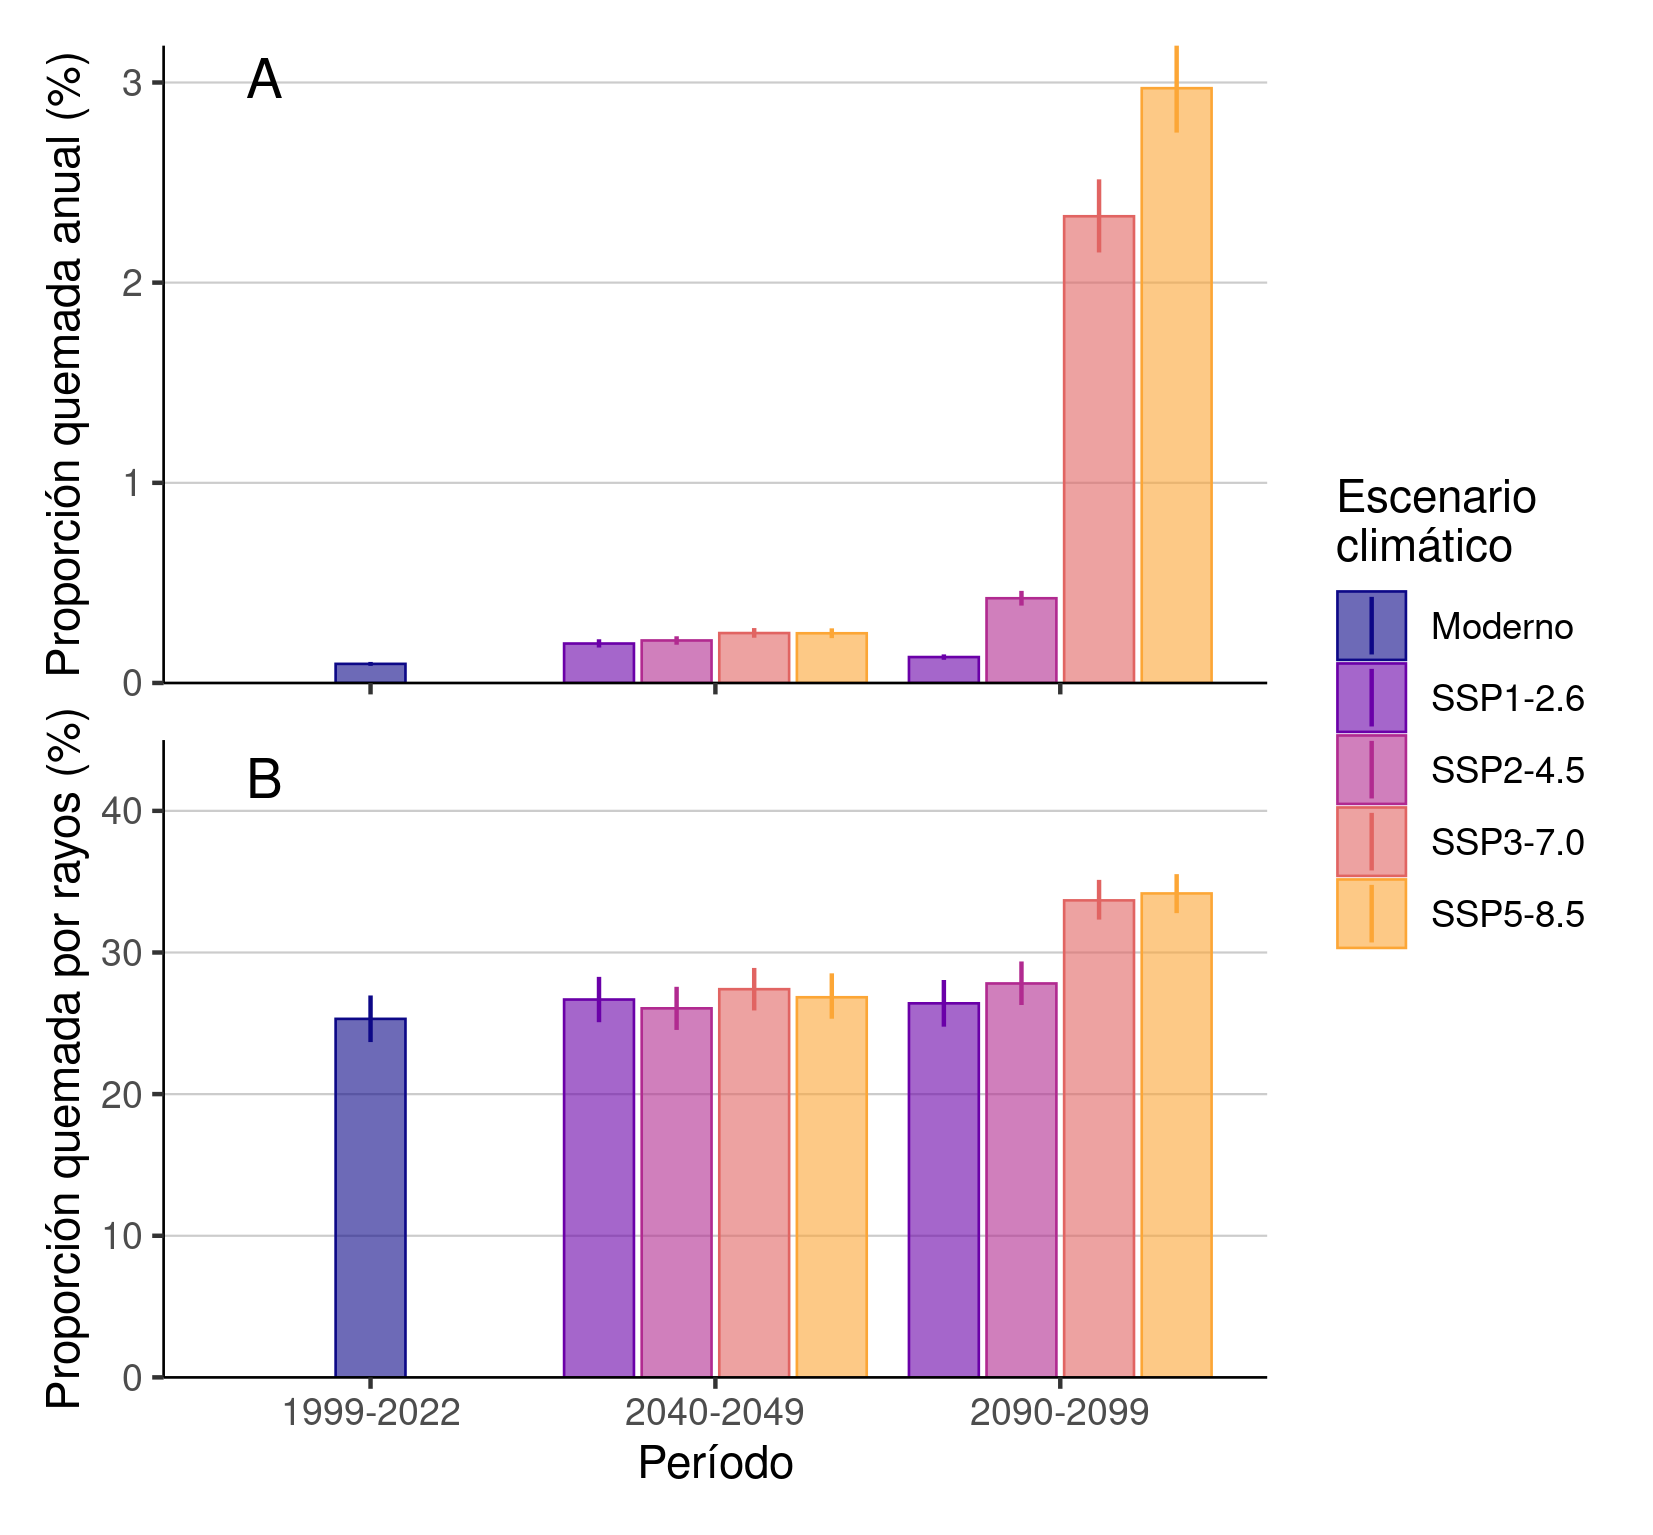
\includegraphics[width=14cm]{figuras/cap4/projections/burn_prob_light_mean_comparison.png}
  \caption[Proporción quemada del PNNH bajo escenarios de clima actual y futuro.]{(A) Proporción quemada de la superficie quemable del PNNH por experimento, y (B) fracción quemada por rayos de la superficie quemada en el PNNH. Las barras muestran la media de la distribución posterior, y las líneas, el intervalo de máxima densidad del 95 \%. Los escenarios climáticos corresponden a trayectorias socioeconómicas compartidas (SSP, por sus siglas en inglés), que representan futuros contrastantes en emisiones y desarrollo socioeconómico, con emisiones de carbono crecientes del SSP1-2.6 al SSP5-8.5 \citep{IPCC2023}.}
  \label{fig:proj-means}
\end{figure}

\begin{figure}[htbp]
  \centering 
  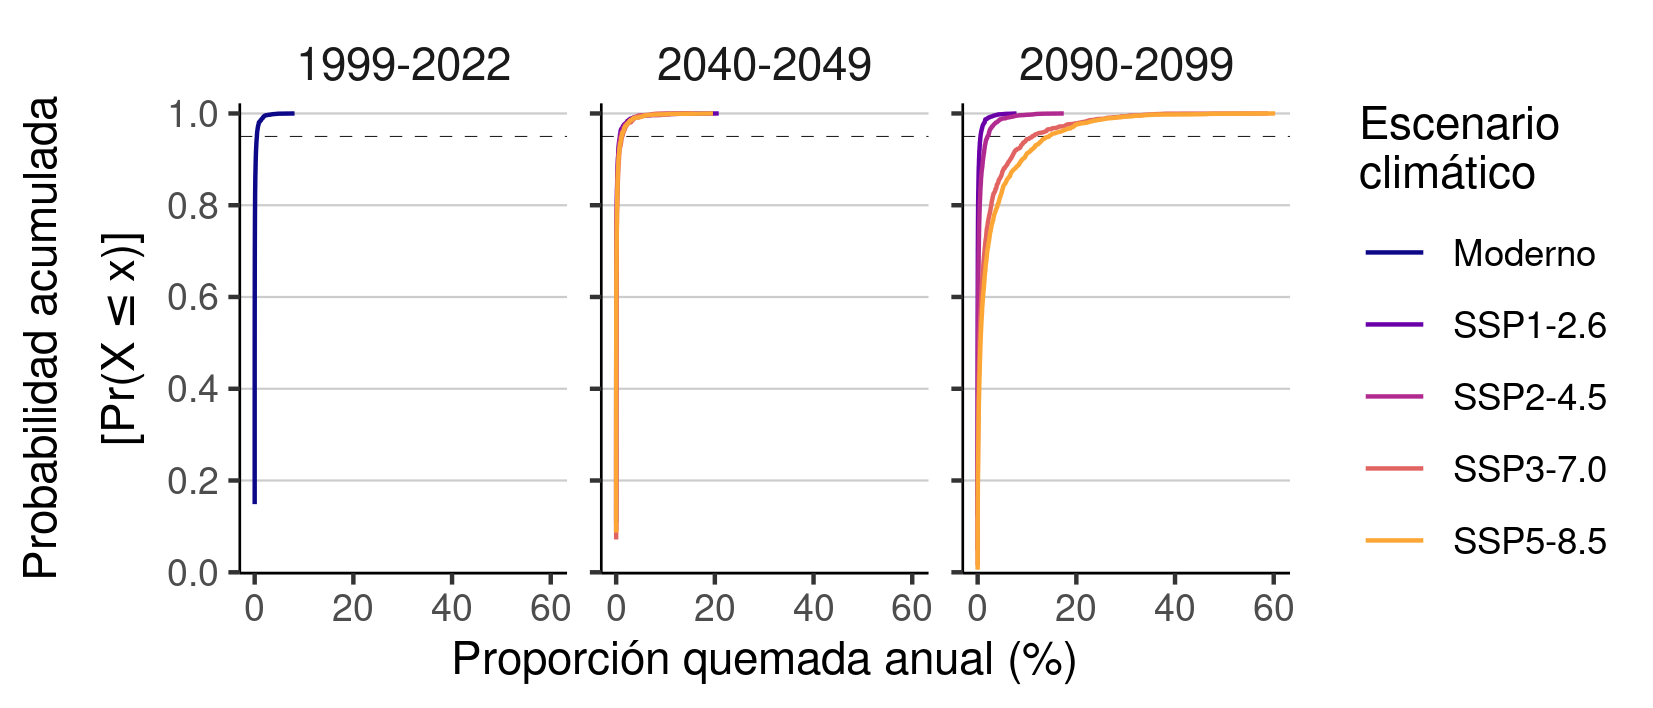
\includegraphics[width=14cm]{figuras/cap4/projections/burn_prob_cdf.png}
  \caption[Distribución de proporción quemada del PNNH bajo escenarios de clima actual y futuro.]{Función de distribución acumulada empírica para la proporción quemada anual del PNNH por experimento. El eje Y indica la probabilidad de que en una simulación la proporción quemada sea menor o igual al valor indicado en el eje X, con la línea discontinua indicando Pr = 0.95. Las curvas se extienden a lo largo del eje X entre el rango observado de proporción quemada. El valor en Y en donde comienzan las curvas indica la proporción de simulaciones sin fuego por experimento.}
  \label{fig:proj-cdf}
\end{figure}


\begin{table}[ht]
\centering
\caption[Proporción quemada del PNNH bajo escenarios de clima actual y futuro.]{Proporción del PNNH quemada anualmente y proporción quemada por rayos sobre el total quemado por experimento. Los factores de cambio son el cociente de la media estimada sobre la media en el período 1999-2022. Los valores representan la media de la distribución posterior, con el intervalo de máxima densidad del 95 \% entre corchetes.}
\label{tab:burn-prob-means}
%\scriptsize % Reduce el tamaño de la fuente
\begin{adjustbox}{max width=\textwidth}
\begin{tabular}{cc|cc|cc}
\toprule
Período & Escenario & \makecell{Proporción quemada\\anual (\%)} & Factor de cambio & \makecell{Fracción quemada\\por rayos (\%)} & Factor de cambio \\
\midrule
1999-2022 & Moderno & 0.1 [0.09; 0.11] & 1 & 25.31 [23.68; 26.96] & 1\\
\addlinespace
\multirow{4}{*}{2040-2049} & SSP1-2.6 & 0.2 [0.18; 0.22] & 2.07 [1.74; 2.35] & 26.68 [25.08; 28.28] & 1.06 [0.96; 1.15]\\
 & SSP2-4.5 & 0.21 [0.19; 0.23] & 2.23 [1.92; 2.55] & 26.06 [24.53; 27.58] & 1.03 [0.94; 1.12]\\
 & SSP3-7.0 & 0.25 [0.23; 0.27] & 2.61 [2.25; 2.98] & 27.41 [25.91; 28.91] & 1.08 [0.99; 1.18]\\
 & SSP5-8.5 & 0.25 [0.22; 0.27] & 2.61 [2.23; 2.98] & 26.84 [25.32; 28.53] & 1.06 [0.97; 1.16]\\
\addlinespace
\multirow{4}{*}{2090-2099} & SSP1-2.6 & 0.13 [0.12; 0.14] & 1.36 [1.17; 1.56] & 26.41 [24.76; 28.06] & 1.04 [0.94; 1.13]\\
 & SSP2-4.5 & 0.42 [0.39; 0.46] & 4.44 [3.87; 5.05] & 27.81 [26.29; 29.37] & 1.1 [1.01; 1.19]\\
 & SSP3-7.0 & 2.33 [2.15; 2.52] & 24.46 [21.44; 27.87] & 33.68 [32.32; 35.13] & 1.33 [1.23; 1.44]\\
 & SSP5-8.5 & 2.97 [2.75; 3.18] & 31.17 [27.53; 35.39] & 34.17 [32.78; 35.53] & 1.35 [1.25; 1.46]\\
\bottomrule
\end{tabular}
\end{adjustbox}
\end{table}

\begin{figure}[htbp]
  \centering 
  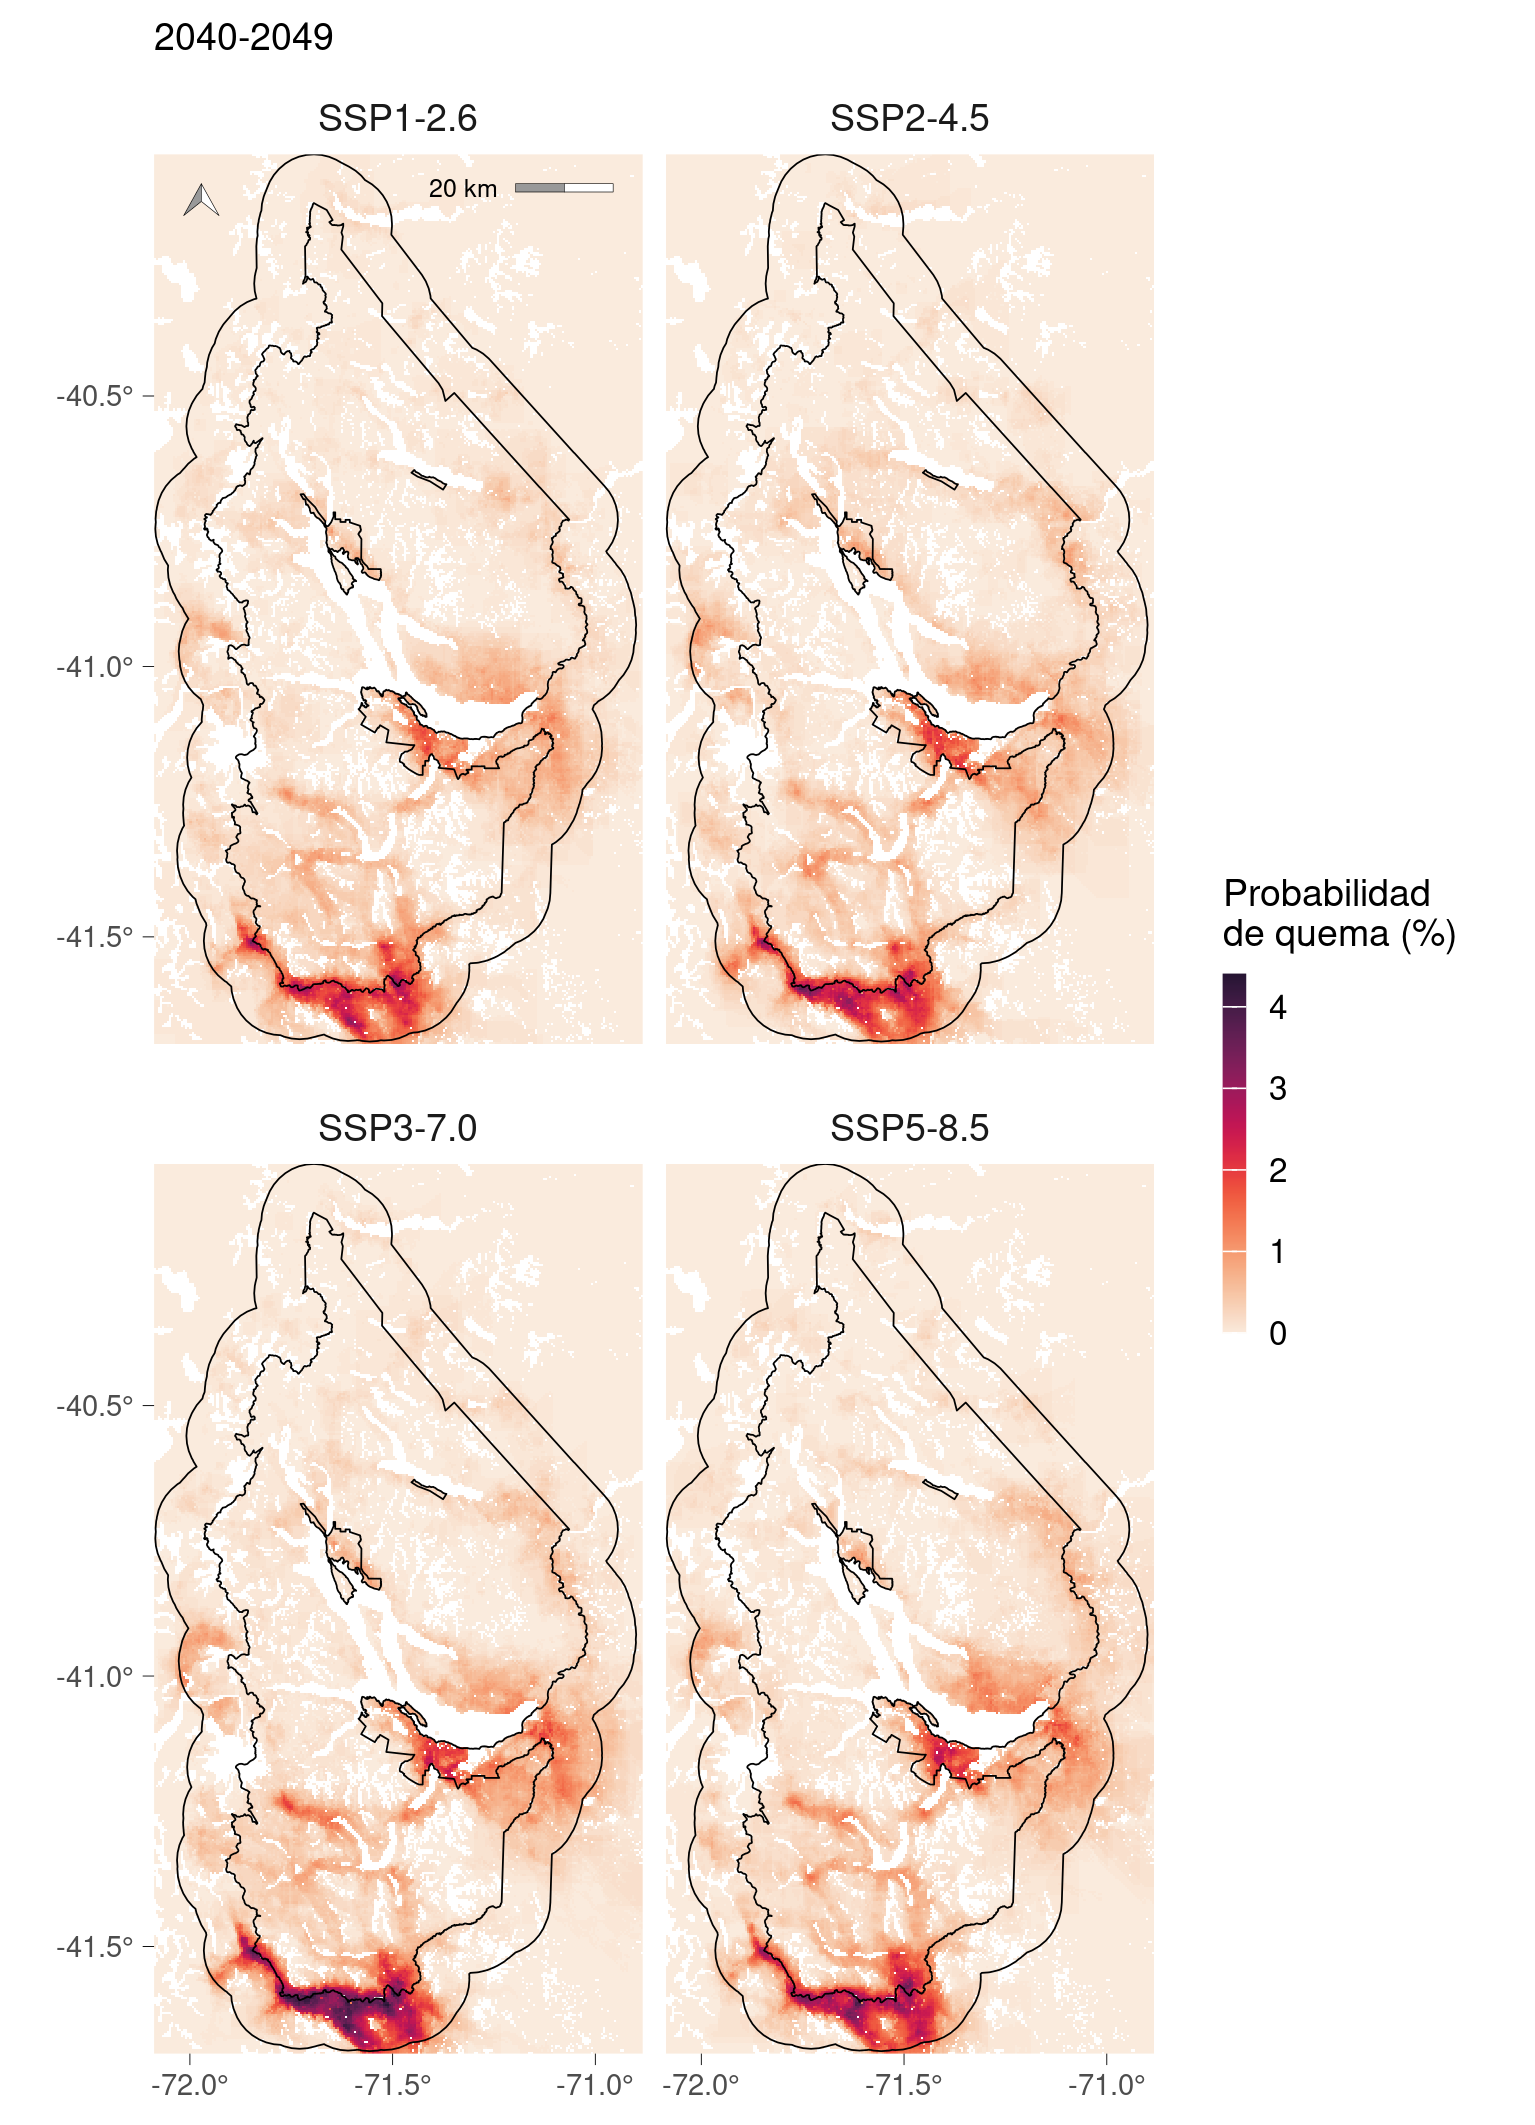
\includegraphics[width=1\textwidth]{figuras/cap4/projections/burn_prob_2040.png}
  \caption[Probabilidad de quema anual en el PNNH proyectada para el período 2040-2049 bajo distintos escenarios climáticos.]{Probabilidad de quema anual en el PNNH proyectada para el período 2040-2049 bajo distintos escenarios climáticos. El contorno exterior indica el área en donde se simularon las igniciones para reducir el efecto borde.}
  \label{fig:proj-2040}
\end{figure}

\begin{figure}[htbp]
  \centering 
  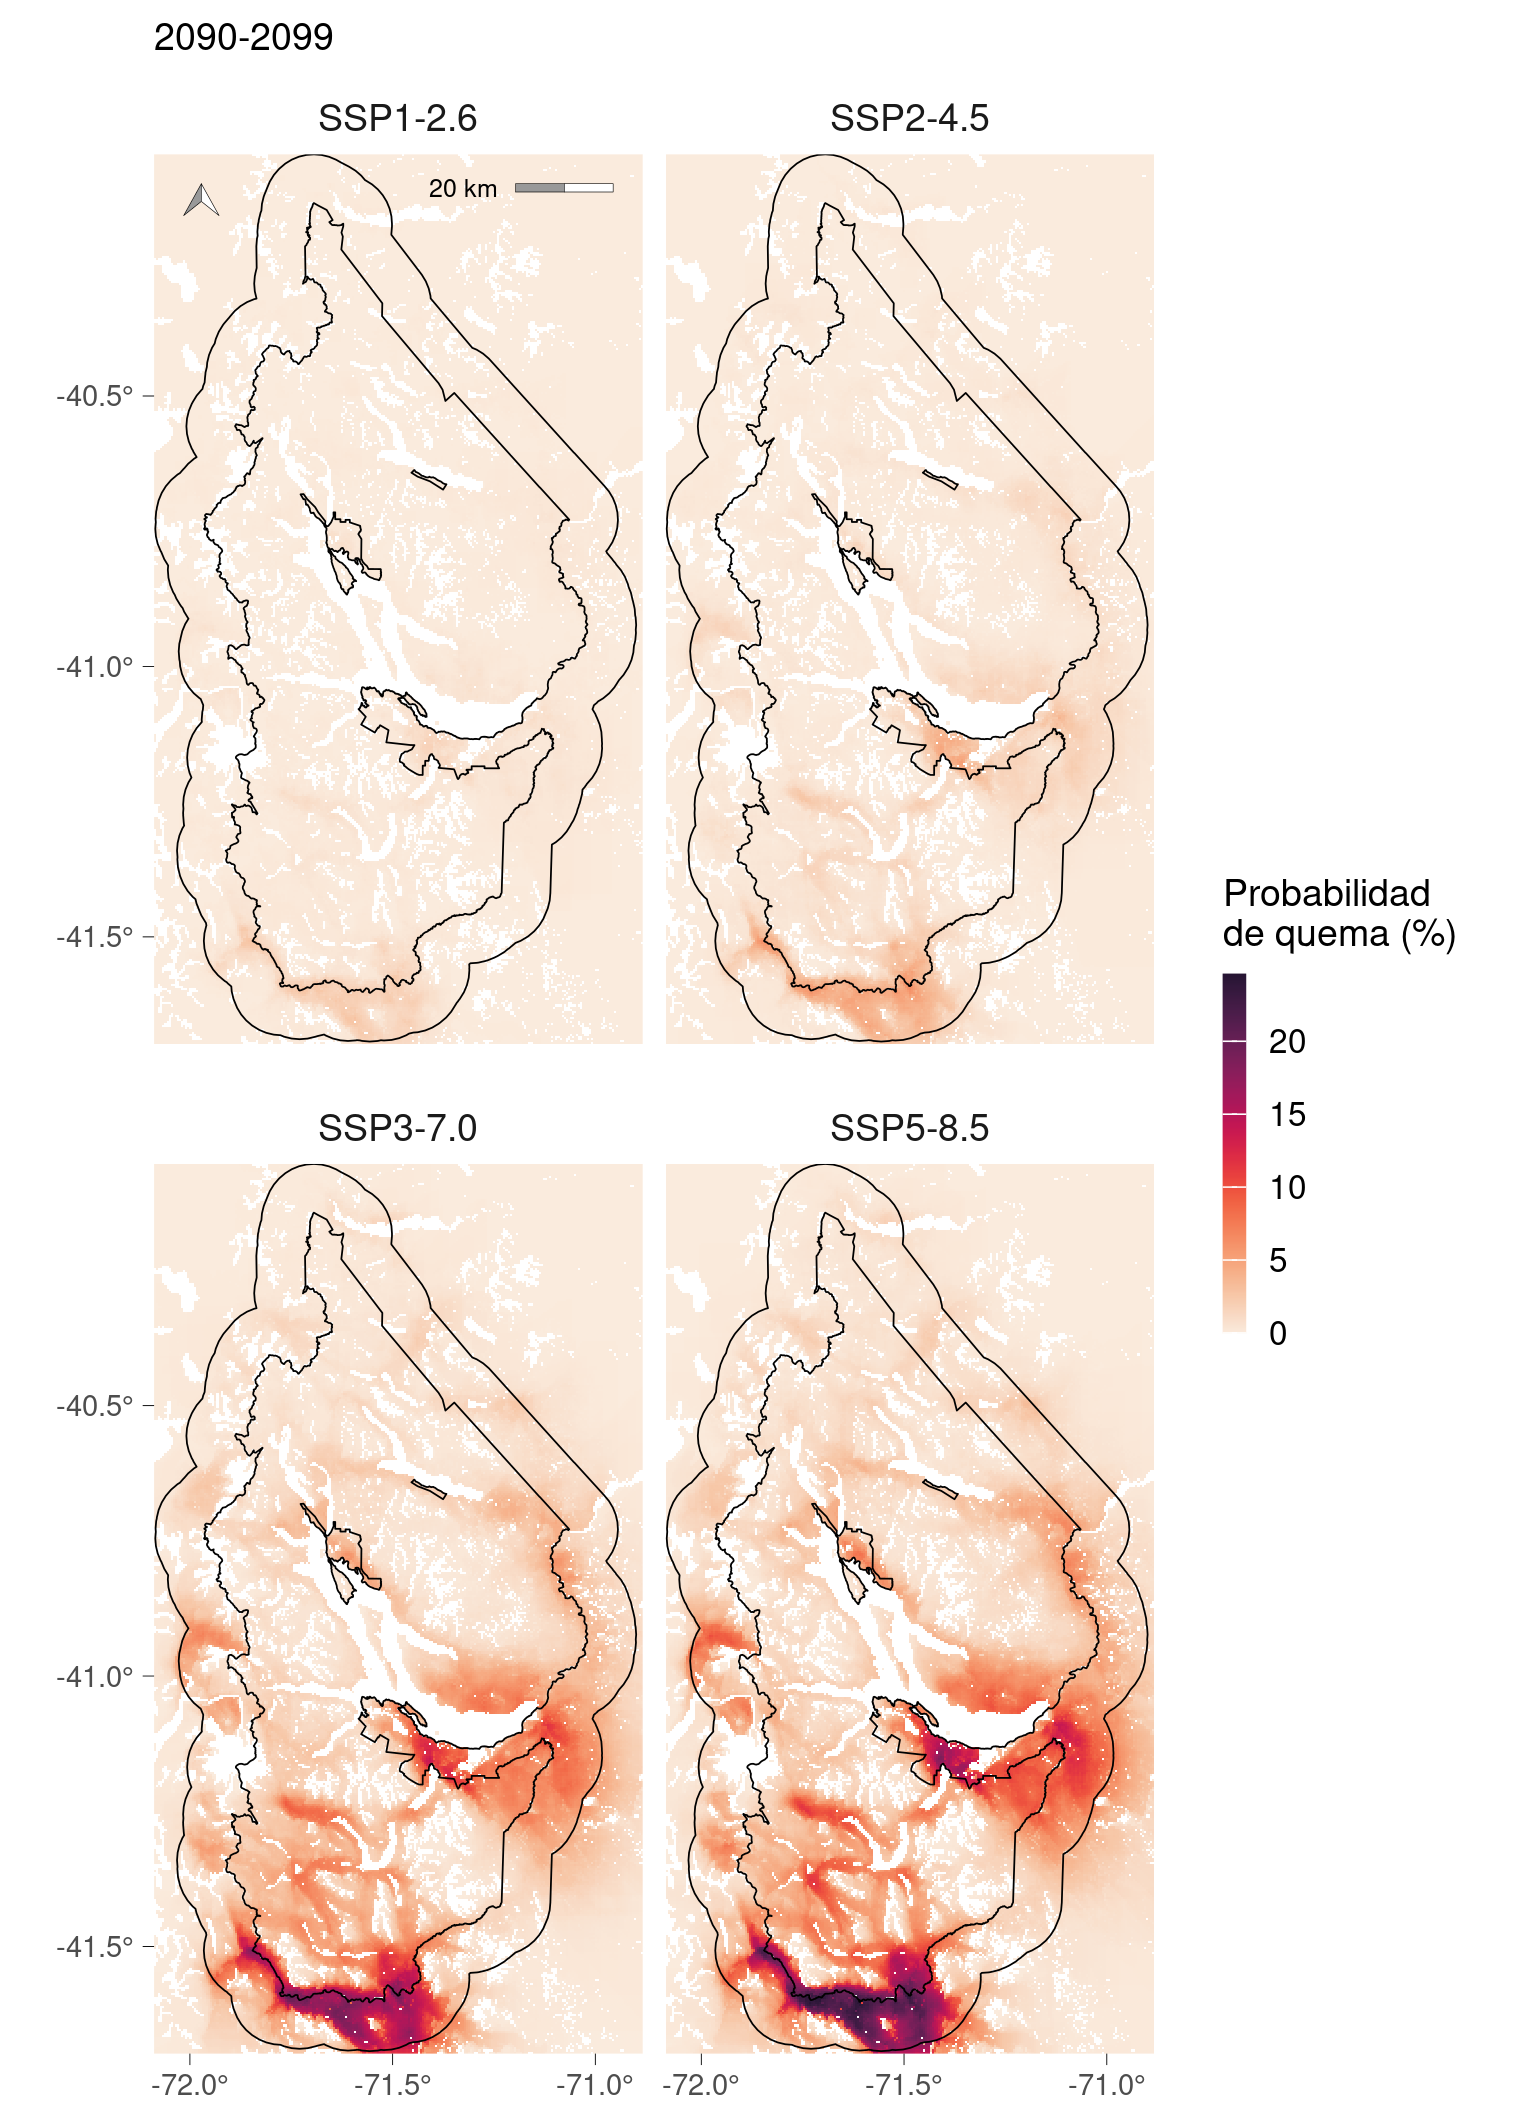
\includegraphics[width=1\textwidth]{figuras/cap4/projections/burn_prob_2090.png}
  \caption[Probabilidad de quema anual en el PNNH proyectada para el período 2090-2099 bajo distintos escenarios climáticos.]{Probabilidad de quema anual en el PNNH proyectada para el período 2090-2099 bajo distintos escenarios climáticos. El contorno exterior indica el área en donde se simularon las igniciones para reducir el efecto borde.}
  \label{fig:proj-2090}
\end{figure}

\FloatBarrier % no projection images below

\section{Discusión}

% overview
En este trabajo desarrollamos modelos de simulación de incendios espacialmente explícitos tomando en cuenta sus principales controles a escala de paisaje, y con ellos estimamos la probabilidad de quema en el PNNH bajo escenarios climáticos futuros. Los resultados sugieren que la incidencia del fuego en esta región se duplicará (2 x) para los 2040s, mientras que para fines de siglo se esperan aumentos menores (1.3 x) o notablemente mayores (31 x), dependiendo del escenario climático.

% discusión modelos puntuales
Los modelos de ignición, escape y propagación reflejaron de forma razonable muchos aspectos conocidos sobre el comportamiento del fuego. Por ejemplo, la tasa de ignición por rayos mostró un aumento más marcado con el FWI que la tasa de ignición por humanos. Esto resulta sensato considerando que, si bien la ocurrencia de focos por ambas causas se relaciona con la meteorología porque dependen de la humedad del combustible, los focos causados por rayos requieren, además, condiciones atmosféricas propicias para la actividad eléctrica \citep{shmuel2024lightning}. En cambio, los focos causados por humanos dependen de la actividad humana, que no necesariamente está tan asociada a condiciones atmosféricas como la ocurrencia de rayos \citep{deDiego2023examining}. A su vez, el aumento en la probabilidad de escape en función de la distancia a caminos y poblados refleja la dificultad para controlar focos remotos \citep{thompson2021forest,kolkos2025evaluation}. 

Quizás los aspectos más llamativos de los modelos desarrollados se encuentren en el modelo de propagación, que al haberse ajustado sin datos de contagio celda a celda, presentaba mayor dificultad para representar la propagación, en comparación con los modelos de ignición y escape. Una de las características más importantes de este modelo es que la probabilidad de propagación depende principalmente de los efectos direccionales del viento y la pendiente, con la vegetación y la topografía (altitud y orientación) tomando roles secundarios \citep{rothermel_mathematical_1972}. Además, la correlación negativa entre los efectos del viento y la pendiente refleja el hecho de que la propagación del fuego tiende a estar dominada por un factor u otro (\citealt{laneri_first_2020}; \cref{fig:spread-corr}). A su vez, el efecto del viento, que representa la velocidad del viento en cada incendio (variable no observada), aumentó con el FWI (Fig.~\ref{fig:spread-params}E); lo cual es coherente con el FWI estando definido como una función creciente de la velocidad del viento, además de la temperatura, humedad del aire, y precipitación. Otro aspecto a destacar fue la correlación positiva entre los pasos de simulación ($\kappa$, ver Ecuación~\ref{eq:datamodel}) y el efecto del viento ($\beta_4$; \cref{fig:spread-corr}): en condiciones de mayor velocidad del viento, los incendios requieren más pasos de simulación, lo que les permite extenderse en la dirección del viento. Esta correlación positiva limita las simulaciones en que el fuego propaga en cualquier dirección durante muchos pasos, lo que generaría incendios extremadamente grandes. 

Si bien el modelo de propagación representó de forma razonable muchos aspectos conocidos sobre la propagación del fuego, su limitada capacidad para simular incendios similares a los ocurridos (utilizando parámetros simulados, Fig.~\ref{fig:spread-ov} y \ref{fig:spread-q}) demuestra que el polígono final y el punto de ignición de los incendios aportan limitada información sobre la propagación. En los últimos años, algunas instituciones encargadas del combate de incendios, como el ICE del PNNH, comenzaron a elaborar polígonos de avance diario de los incendios. A su vez, recientemente se han instalado numerosas estaciones meteorológicas en la región. Con estas nuevas fuentes de datos podremos desarrollar y estimar modelos de propagación más realistas, modelando los efectos del viento y la pendiente sobre la propagación del fuego a mayor resolución temporal y espacial, lo que permitirá cuantificar en forma más detallada el efecto de variables con efectos menos marcados, como la vegetación y la topografía. 

% vegetación

A pesar de la simpleza del modelo de propagación, aportó evidencia relevante desde un punto de vista ecológico: el efecto de la vegetación (IIV) no varió a lo largo de un amplio rango de FWI (Fig.~\ref{fig:spread-curves}A, \ref{fig:spread-params}A y \ref{fig:spread-veg-effects}). Numerosos estudios reportan que los controles locales del fuego (\textit{bottom-up}), como la vegetación y la topografía, tienden a atenuarse bajo condiciones atmosféricas extremas: tipos de combustible o condiciones topográficas que que normalmente limitan la propagación del fuego, pueden dejar de ser una barrera efectiva y permitir una mayor propagación bajo condiciones atmosféricas extremas \citep{Podur2009, Parks2015, Collins2019, jones_extreme_2023}. Sin embargo, encontramos que el efecto de la vegetación, a pesar de ser un control secundario de la probabilidad de propagación, se mantuvo para valores altos de FWI. Esto podría reflejar que, si bien todos los tipos de vegetación pueden arder cuando las condiciones atmosféricas lo permiten, la velocidad de propagación del fuego aún es menor en comunidades boscosas cerradas, debido al mayor contenido de humedad del combustible, su menor continuidad, y la mayor carga de combustibles gruesos que actúan como sumideros de calor \citep{zylstra_biophysical_2016}. Si bien sería esperable que a valores de FWI mayores a los observados en el período de los datos (1998-2022) la probabilidad de propagación tienda a 1 para todos los tipos de vegetación, anulando su efecto, la vegetación aún presenta un control importante para el fuego ante un FWI elevado. Esto resulta relevante a la hora de considerar estrategias de manejo: conservar comunidades boscosas con dosel alto y cerrado podría disminuir la velocidad de propagación del fuego en el paisaje, lo cual disminuiría el área quemada en comparación con paisajes dominados por matorrales \citep{tiribelli_non-additive_2019}. 

% performance

Evaluar el desempeño de modelos de probabilidad de quema (como nuestro simulador del régimen de incendios) es desafiante porque producen salidas a escalas temporales y espaciales amplias (e.g., probabilidad de quema en un área extensa y sobre muchos años), por lo que es dificultoso imposible contar con datos para evaluarlos \citep{parisien2020commentary}. En nuestro caso, utilizamos toda la (escasa) información disponible para ajustarlos, y prácticamente no tenemos información independiente para juzgarlos. A su vez, estos modelos no buscan predecir con precisión eventos puntuales, como dónde se quemará en un año en particular, sino representar posibles características del régimen de incendios ante distintos escenarios. Debido a estas particularidades, este tipo de modelos se evalúa juzgando su solidez conceptual y su utilidad para la toma de decisiones, más que por su capacidad para reproducir incendios observados durante períodos cortos \citep{parisien2020commentary}. Aún así, podemos evaluar si el simulador del régimen de incendios recupera patrones generales observados en los datos.

Siguiendo esta lógica, observamos que la probabilidad de quema anual en el PNNH para el período de los datos (1999-2022) presenta un patrón espacial similar a los resultados del Capítulo~\ref{cap:patrones}, donde la altitud fue uno de los factores más importantes regulando la probabilidad de quema. Sin embargo, algunos aspectos de las simulaciones no parecen tener una buena adecuación a los datos. Por un lado, es probable que la contribución relativa de las igniciones por rayos al área quemada esté subestimada. Para 1999-2022 los modelos estimaron un $\approx$ 25 \% (Fig.~\ref{fig:proj-means}B, Tabla~\ref{tab:burn-prob-means}). Este valor se encuentra dentro del rango registrado para las últimas tres décadas en cuatro parques nacionales de la zona (PNNH, Los Alerces, Lago Puelo y Lanín), con 17 \%, 25 \% y 50 \% en las décadas centradas en 2000, 2010 y 2020, respectivamente (\citeauthor{kitzbergerLightning}, en revisión). Para 1999-2022 pero en el área más extensa estudiada en el Capítulo~\ref{cap:patrones}, no contamos con datos de causa para todos los incendios, pero los dos más grandes, que acumulan casi el 30 \% del área quemada, fueron causados por rayos (San Ramón 1999 y Cholila 2015), sin contar otros de gran extensión también causados por rayos. En el PNNH y en el mismo período no contamos con la causa de algunos de los fuegos más grandes, pero la contribución relativa de rayos sería de al menos 46.83 \%. Sin embargo, este valor fue altamente influido por el fuego más grande registrado en el período (Complejo Steffen-Martin 2022). A su vez, el reciente incendio de Los Manzanos (sur del PNNH, verano de 2025), causado por un rayo, constituye uno de los más grandes registrados en el PNNH, aumentando aún más la contribución relativa de los rayos. Si bien la contribución al área quemada de cada fuente de igniciones (rayos-humanos) requiere muchos años de datos porque depende fuertemente de eventos extremos, los modelos aquí desarrollados parecen subestimar la importancia de los rayos en el área quemada total. Esto probablemente se deba a que los incendios generados por rayos, ocurriendo lejos de caminos y poblados, presentan una alta dificultad para el combate no sólo en su momento inicial, sino en todo su desarrollo \citep{thompson2021forest,kolkos2025evaluation}. Nuestros modelos sólo consideran esta mayor dificultad aumentando su probabilidad de escape. Una forma de mejorar este aspecto sería incluir la distancia a caminos y a poblados como predictoras del número de pasos de simulación ($\kappa$) en el modelo de propagación. A su vez, más allá de nuestra posible subestimación de la contribución de relativa de los rayos al área quemada para el período 1999-2022, los aumentos bajo clima futuro parecen presentar problemas mayores. Las condiciones atmosféricas de verano se están volviendo más favorables para la ocurrencia de tormentas eléctricas y para las igniciones por rayos (\citeauthor{kitzbergerLightning}, en revisión), con lo cual, los aumentos proyectados, en factores de $1.06$ y $1.3$ para mediados y fines de siglo, respectivamente (Table~\ref{tab:burn-prob-means}), resultan poco probables, salvo que esperemos un notable aumento en los recursos invertidos en prevención, detección y combate del fuego.

Otro aspecto en que los modelos discrepan de los datos es en la elevada probabilidad de quema predicha en el valle del Manso Inferior, al sur del PNNH. En el periodo de estudio no registramos incendios en esa zona, lo que puede reflejar particularidades de uso humano que resultan en una tasa de ignición por humanos mucho menor que la esperada a esa altitud. Sin embargo, como mencionamos arriba, 24 años de datos en una región con baja incidencia de fuego es poco para juzgar las predicciones de este tipo de modelos \citep{parisien2020commentary}; la ausencia de incendios en esa zona podría ser simplemente azar. De hecho, en el verano de 2025 el incendio de Los Manzanos, generó un foco secundario que llegó a la zona del Valle del Manso Inferior (incendio El Manso).

% proyecciones 

Nuestras proyecciones de proporción quemada y probabilidad de quema anual se asemejan cualitativamente a los resultados de \citet{kitzberger_projections_2022} para un área más extensa (similar al área de estudio del Capítulo~\ref{cap:patrones}; Fig.~\ref{fig:cap3-01}). En dicho trabajo ajustamos un Random Forest para predecir la probabilidad de quema anual de cada celda en el paisaje en función de variables topográficas, de vegetación, climáticas, indicadores de influencia humana y variables atmosféricas, basado en el producto de área quemada de MODIS \citep{giglio_collection_2018}. Si bien los patrones son similares, en dicho trabajo encontramos mayor variación entre escenarios climáticos para el período 2041-2050. Además, para el período 2091-2100, en \citet{kitzberger_projections_2022} reportamos aumentos notablemente menores, alcanzando un valor de 8 x en algunas partes del paisaje bajo el escenario RCP 8.5 (equivalente a SSP5-8.5), comparado con el aumento máximo de 31 x que encontramos en este trabajo. Aunque parte de la discrepancia puede deberse a diferencias en las bases de datos utilizadas, probablemente se explique principalmente por el modelo utilizado en \citet{kitzberger_projections_2022}. Proyectar probabilidad de quema bajo clima futuro es una tarea de extrapolación, y los Random Forests no son una herramienta adecuada para tal fin, ya que en su formulación clásica sólo pueden predecir valores tan altos como el máximo predicho en el set de datos de entrenamiento (\citealt{zhang2019_RF_enhanced}). Sin habernos percatado de la dificultad de extrapolar, nuestros modelos de simulación inicialmente presentaban el problema opuesto: utilizando funciones exponenciales, el clima futuro quemaba todo el paisaje con facilidad, lo que nos llevó a utilizar funciones sigmoideas (Ecuaciones~\ref{eq:igrate} y \ref{eq:hier1}) para obtener proyecciones razonables. Estos aspectos resaltan los desafíos de realizar proyecciones bajo condiciones climáticas que no fueron previamente observadas \citep{fitzpatrick2018will}. 

Si bien nuestro enfoque de modelado contrasta con el empleado en \citet{kitzberger_projections_2022} porque descompusimos en más subprocesos la ocurrencia del fuego (ignición, escape y propagación), las proyecciones bajo clima futuro de ambos trabajos comparten una limitación: en ambos casos proyectamos el régimen de incendios ignorando la retroalimentación entre fuego y vegetación. En nuestras simulaciones, e implícitamente en las proyecciones de \citet{kitzberger_projections_2022} suponemos que la vegetación se mantiene intacta luego de ser quemada, pudiendo quemarse nuevamente al año siguiente, sin considerar regeneración, sucesión, ni transiciones hacia otros tipos de vegetación. Nuestros modelos de simulación fueron concebidos con el objetivo de ser integrados en un modelo dinámico de vegetación que permita modelar explícitamente esta retroalimentación, pero hasta que dicho modelo sea implementado, debemos evaluar con cautela las proyecciones basadas en una capa de vegetación que se reinicia en cada simulación. En esta región, ignorar los efectos de la vegetación puede tener dos efectos opuestos. Primero, si cada año de simulación utiliza vegetación en su mayoría no quemada y, por lo tanto, quemable, la probabilidad de quema se puede sobrestimar, ya que la vegetación puede tardar entre 2 y 20 años en recuperarse y poder propagar fuego con facilidad \citep{tiribelli_changes_2018, tiribelli_non-additive_2019}. Pero esto sería problemático únicamente en zonas o escenarios climáticos en donde el intervalo de retorno del fuego es corto. Bajo clima actual, la zona con mayor probabilidad de quema anual (Manso Inferior) alcanza el 2 \%, lo que implica un retorno medio de 50 años ($1/0.02$); para 2040-2049, en esa zona se proyecta una probabilidad de quema del 4 \%, implicando un intervalo de retorno de 25 años, y para 2090-2099, el tiempo de retorno sería de 4 años. En casos como los últimos dos, la probabilidad de quema probablemente esté ligeramente sobrestimada, pero no en el resto del paisaje, donde la probabilidad de quema es notablemente menor. El otro efecto de asumir vegetación estática es que se ignoran las transiciones hacia otros tipos de vegetación tras el paso del fuego \citep{kitzberger_firevegetation_2016}. Los bosques tienden a ser reemplazados por matorrales si el fuego no deja semilleros vivos a cortas distancias \citep{landesmann_importance_2018,landesmann_increased_2021}, lo cual es frecuente \citep{tiribelli2024spatial}, y si las precipitaciones son escasas \citep{cuevas_tree_2000,kitzberger_effects_2005,tercero-bucardo_field_2007}, que, a su vez, están disminuyendo con el cambio climático (Tabla~\ref{tab:climate-ts}). De esta manera, es probable que nuestras proyecciones sean conservativas, ya que la transición de bosques a matorrales aumentaría la inflamabilidad del paisaje (\citealt{mermoz_landscape_2005,paritsis_positive_2015,morales_stochastic_2015,tiribelli_changes_2018,tiribelli_non-additive_2019}; Capítulo~\ref{cap:patrones}). A su vez, más allá de las transiciones de bosque a matorral causadas por fuego, el cambio climático podría aumentar la inflamabilidad de los bosques a través de los efectos a mediano y largo plazo de las sequías. La mayor frecuencia y severidad de sequías puede aumentar la mortalidad de los árboles que conforman el dosel y la mortalidad parcial de copa \citep{suarez2004factors,rodriguez2016influence,molowny2017changes}. Esto disminuiría la cobertura del dosel, pudiendo resultar en menor humedad de combustible \citep{barbera_microclimate_2023} y promoviendo el desarrollo de la vegetación del sotobosque, lo que aumentaría la continuidad del combustible. Además, esto aumentaría la cantidad de combustible muerto en pie. Pero estos aspectos deben ser analizados con modelos dinámicos de vegetación, ya que también se debe considerar cómo el aumento en la concentración de $\text{CO}_2$ atmosférico puede aumetar la eficiencia fotosintética de las plantas, haciéndolas más tolerantes a las altas temperaturas y a las sequías \citep{silva2013probing,sperlich2020gains}. Este proceso, podría atenuar la mayor mortalidad de árboles que se espera bajo clima futuro \citep{gutierrez2014increased,sperlich2020gains}.

% implicancias-manejo

Si bien nuestras proyecciones ofrecen un escenario posible bajo ciertas condiciones climáticas y sociales, es importante remarcar que en este trabajo suponemos que la tasa de ignición humana y la eficiencia de la prevención y control del fuego se mantienen como en el período 1999-2022). Esto podría implicar una notable sobreestimación de la incidencia del fuego si, en las próximas décadas, se lograran avances significativos en la reducción de igniciones humanas, en la detección temprana de incendios causados por rayos y en el combate. Sin embargo, también es necesario considerar que nuestras proyecciones no incorporan el probable aumento en la frecuencia de tormentas eléctricas (\citeauthor{kitzbergerLightning}, en revisión), lo que volvería aún más improbable un escenario optimista si no se contrarresta con mejoras sustanciales en el combate del fuego. En este contexto, disminuir las igniciones por humanos debería ser una de las estrategias más convenientes. Sin embargo, las igniciones humanas están asociadas a condiciones socioeconómicas desfavorables (e.g., alta tasa de desempleo) y a una alta densidad poblacional \citep{buhler2013demography}, por lo que se requerirían políticas de largo plazo para reducirlas, no sólo campañas de prevención en la estación seca en formato de propaganda. Un ejemplo cercano que ilustra la dificultad de reducir las igniciones antrópicas son las sierras de Córdoba. En dicha región se quema entre un 1.3 y un 3.2 \% del paisaje anualmente (\citealt{arganaraz_incidencia_2020}; cercano a los peores escenarios climáticos para PNNH en los 2090s), y la gran mayoría de los incendios son causados por humanos.

% (párrafo viejo :)

% Una mayor incidencia de incendios generaría mayor gasto en minimizar los daños a la vida humana y la infraestructura, y probablemente generaría una transformación del bosque andino-patagónico, perdiendo representatividad de comunidades boscosas a favor de una mayor abundancia de matorrales \citep{kitzberger_firevegetation_2016,kitzberger_projections_2022}. Las igniciones por rayos aumentarán con el cambio climático (\citealt{perez2023variation}, \citeauthor{kitzbergerLightning}, en revisión) y no pueden ser evitadas, con lo cual se debería invertir en su rápida detección y en aumentar la efectividad del combate inicial para reducir sus impactos. En comparación, disminuir las igniciones por humanos debería ser más factible. Sin embargo, las igniciones humanas están asociadas a condiciones socioeconómicas desfavorables (e.g., alta tasa de desempleo) y a una alta densidad poblacional \citep{buhler2013demography}, por lo que se requerirían políticas de largo plazo para reducirlas, no sólo campañas de prevención en la estación seca en formato de propaganda. Un ejemplo cercano que ilustra la dificultad de reducir las igniciones antrópicas son las sierras de Córdoba. En dicha región se quema entre un 1.3 y un 3.2 \% del paisaje anualmente (\citealt{arganaraz_incidencia_2020}; cercano a los peores escenarios climáticos para PNNH en los 2090s), y la gran mayoría de los incendios son causados por humanos.

% fin

Este trabajo presenta un avance considerable en los esfuerzos de modelado para predecir y proyectar la incidencia del fuego y los patrones de vegetación en el norte de la Patagonia Andina. En el futuro podremos integrar distintos modelos en una plataforma que permita su continua actualización y validación (e.g., \texttt{SpaDES}; \citealt{barros2023empowering, SpaDES}). Para generar proyecciones confiables, será necesario avanzar en el entendimiento de la relación entre condiciones atmosféricas y la incidencia de rayos, los factores que regulan las igniciones humanas, y las respuestas de la vegetación al cambio climático, tanto mediadas por fuego como por otros factores. 
\newpage{\ }
\cleardoublepage

\chapter[Capítulo 5. Discusión general]{Discusión general}\label{cap:discu}

En esta tesis avanzamos el entendimiento de los factores que controlan el fuego en el norte de la Patagonia Andina argentina a diversas escalas temporales y espaciales, aportando evidencia a partir de un estudio de campo y del análisis de la ocurrencia de incendios a escala de paisaje. En particular, pudimos separar efectos del tipo de vegetación de factores ambientales asociados. Finalmente, integramos lo aprendido en modelos de simulación de incendios, que permitieron proyectar la incidencia del fuego en la región bajo escenarios climáticos futuros. 

Un factor común a lo largo de esta tesis fue la contrastante inflamabilidad entre bosques y matorrales, observada a distintas escalas. A escala de sitio, los matorrales presentaron mayor probabilidad de ignición de combustibles muertos debido a su menor contenido de humedad comparado con los bosques (Fig.~\ref{fig:cap2-06}); a escala de paisaje, los matorrales mostraron mayor probabilidad de quema comparados con comunidades boscosas, incluso controlando por factores ambientales correlacionados (Fig.~\ref{fig:cap3-06}C). Estas diferencias también emergieron al modelar por separado la ignición, escape y propagación del fuego: los matorrales presentaron mayor probabilidad de ignición y de propagación que los bosques (Fig.~\ref{fig:ig_spat_veg} y ~\ref{fig:spread-veg-effects}). Estudios previos ya habían reportado diferencias estructurales que harían a los matorrales más inflamables que los bosques \citep{paritsis_positive_2015, blackhall_effects_2017, tiribelli_changes_2018}, y a escala de paisaje, los matorrales mostraban mayor probabilidad de quema \citep{mermoz_landscape_2005, paritsis_habitat_2013, morales_stochastic_2015}. Sin embargo, estos estudios presentaban algunas limitaciones para evaluar diferencias en inflamabilidad entre estos tipos de vegetación. Por un lado, las diferencias estructurales entre matorrales y bosques podrían perder relevancia bajo condiciones atmosféricas extremas \citep{Podur2009, Parks2015, Collins2019, jones_extreme_2023}, y por otro lado, la mayor probabilidad de quema de los matorrales observada a escala de paisaje podría estar explicada, al menos en parte, por otros factores correlacionados con el tipo de vegetación, como altitud -que influye en la temperatura-, precipitación, y uso humano. En esta tesis evaluamos estos aspectos, y encontramos que (1) los tipos de vegetación presentan inflamabilidad contrastante incluso bajo condiciones atmosféricas extremas (Fig.~\ref{fig:ig_spat_veg}), y (2) aún controlando por factores físicos o de uso humano a escala de paisaje, los matorrales sobresalen como una de las comunidades más inflamables (Fig.~\ref{fig:cap3-06}C). A su vez, encontramos que los bosques pueden presentar inflamabilidad similar a la de los matorrales cuando tienen baja productividad (bajo NDVI; Fig.~\ref{fig:cap3-05}B y \ref{fig:FI}A), probablemente porque presentan doseles abiertos, lo que les confiere características similares a las de los matorrales en cuanto a humedad y continuidad del combustible. 

La mayor inflamabilidad de los matorrales y bosques de baja productividad tiene implicancias relevantes para el fuego si consideramos los efectos del cambio climático sobre la vegetación. Ante un clima más cálido y seco, la regeneración posfuego de los bosques se verá limitada \citep{tercero-bucardo_field_2007}, aumentando la probabilidad de que sean reemplazados por matorrales a altitud baja e intermedia y por pastizales en la franja altitudinal superior \citep{kitzberger_firevegetation_2016, kitzberger_projections_2022}. A su vez, estas condiciones climáticas promueven el decaimiento y la mortalidad de árboles (ya sea parcial o total; \citealt{suarez2004factors,gutierrez2014increased,rodriguez2016influence,molowny2017changes}), con lo cual, los bosques pueden volverse más abiertos. Esto aumentaría la tasa de desecación de combustibles muertos y la continuidad de combustibles finos en el sotobosque, aumentando la inflamabilidad. Además, aumentaría la cantidad de combustible muerto en pie. De esta manera, sería esperable que el paisaje se vuelva más inflamable. Sin embargo, hay que tener en cuenta que con el cambio climático el aumento de $\text{CO}_2$ atmosférica podría aumentar la eficiencia hídrica de las plantas, pudiendo atenuar, los efectos del clima sobre la mortalidad \citep{silva2013probing,sperlich2020gains}.

El notable efecto de la vegetación sobre el fuego sugiere que, en las zonas accesibles, se podrían aplicar estrategias de manejo para reducir la inflamabilidad del paisaje. En particular, promover la formación de doseles altos y cerrados podría contribuir a mantener una mayor humedad del combustible  y reducir su continuidad en el sotobosque, disminuyendo así la probabilidad de ignición y propagación del fuego. Esto podría lograrse a través del manejo de matorrales, promoviendo el desarrollo de árboles de un solo fuste, y plantando individuos de especies de gran porte, como coihue, lenga y ciprés, u otras de menor porte pero con elevado contenido de humedad, como maitén. A su vez, la reducción de la biomasa del sotobosque mediante la extracción controlada de leña y madera, en combinación con el pastoreo de ganado, podría contribuir a disminuir la carga de combustible fino. Sin embargo, se deben seguir desarrollando e investigando estrategias de manejo para compatibilizar objetivos de disminución del peligro de incendios y rentabilidad económica \citep{peri_review_2016, goldenberg_efecto_2018, goldenberg_effects_2020, goldenberg_shrubland_2021}. Por otro lado, la elevada inflamabilidad de las plantaciones de coníferas exóticas y de los sitios que estas invaden resalta la necesidad de manejar los combustibles de las plantaciones y controlar las invasiones para disminuir la inflamabilidad del paisaje \citep{paritsis_pine_2018, cingolani2023enrichment, franzese_legacy_2022}.

Más allá del notable control del fuego por parte de la vegetación, las condiciones atmosféricas resultaron ser uno de los factores más influyente en la ocurrencia de incendios (Fig.~\ref{fig:cap3-03}, \ref{fig:igrate}, \ref{fig:spread-params}, y \ref{fig:proj-means}). Con el cambio climático, las condiciones atmosféricas propicias para el fuego serán cada vez más frecuentes y severas. A su vez, esto se agravará con la creciente incidencia de rayos, los cuales generan focos en zonas remotas que resultan muy difíciles de controlar (\citeauthor{kitzbergerLightning}, en revisión). Ante este escenario, será necesario invertir en estrategias de detección y supresión temprana de focos generados por rayos antes de que las condiciones atmosféricas generen incendios de gran tamaño e intensidad que limiten su control. A su vez, reducir considerablemente las igniciones humanas sería altamente beneficioso, para que los recursos destinados a la supresión del fuego puedan destinarse principalmente a los inevitables incendios generados por rayos. Estudios en otras regiones sugieren que las igniciones por humanos pueden ser reducidas notablemente mediante campañas educativas \citep{hesseln_wildland_2018}. Sin embargo, algunos incendios intencionales ocurren bajo condiciones atmosféricas extremas buscadas por sus perpetradores con el fin de generar un gran impacto. Esto sugiere que las tensiones entre distintos actores sociales deberían ser consideradas a la hora de buscar reducir las igniciones por humanos \citep{buhler2013demography}.

Además del fuerte control climático sobre la incidencia del fuego, en el Capítulo~\ref{cap:patrones} encontramos una marcada variabilidad espacial espacial en la incidencia del fuego (Tabla~\ref{tab:cap3-spatvar}). Estas diferencias tan grandes en la proporción del paisaje quemada en las distintas regiones probablemente no se explique únicamente por sus diferencias en topografía y vegetación, sino que podrían estar asociadas a diferencias en el manejo del fuego. De ser así, evaluar en detalle por qué algunas regiones se queman más que otras, en relación a los recursos destinados a la prevención y control del fuego, y al uso intencional del fuego por parte de las personas podría informar estrategias relevantes para disminuir la incidencia del fuego. 

Pero incluso considerando mejores estrategias para prevenir y controlar el fuego, el aumento previsto en la incidencia del fuego a causa del cambio climático y la dificultad para disminuir las igniciones humanas sugiere que estas estrategias probablemente no sean suficientes. Además, se requerirán estrategias para atenuar el inevitable impacto del fuego sobre las sociedades. En particular, esto podría lograrse implementando estrategias de evacuación ante incendios \citep{cova2002microsimulation}, promoviendo la construcción de infraestructura poco inflamable \citep{quarles2010home} y manejando la vegetación en las cercanías de la infraestructura humana, disminuyendo la biomasa de combustibles y plantando especies con un alto contenido de humedad \citep{reinhardt2008objectives, syphard2014role, blackhall_flammability_2019}. A su vez, a una escala temporal mayor, se podría diseñar un paisaje en donde las viviendas se acumulen en zonas poco vegetadas en vez de seguir desarrollando una amplia interfaz urbano-forestal en donde las viviendas se encuentran altamente expuestas al fuego \citep{syphard2013land, moritz2014learning, barrett2019reducing}. Sin embargo, políticas de este tipo probablemente sean más difíciles de implementar, requiriendo una fuerte presencia del Estado.   

El estudio del fuego y la vegetación con un enfoque de modelado espacialmente explícito puede realizar importantes contribuciones al manejo de los ecosistemas del norte de la Patagonia Andina argentina. En particular, las proyecciones de la dinámica de la vegetación y el fuego en esta región probablemente sean más atinadas avanzando nuestro entendimiento de los siguientes aspectos: 

\begin{itemize}
    \item factores que controlan la incidencia de rayos y cómo la misma se verá afectada por el cambio climático;
    \item efectos de la sequía sobre la inflamabilidad de los bosques;
    \item dinámica de la vegetación (incluyendo regeneración posfuego) ante un clima más cálido y seco;
    \item dinámica de floración de la caña \textit{Chusquea culeou}, cuyos eventos de floración y seguida mortalidad sincronizada aumentan la inflamabilidad del paisaje dramáticamente;
    \item dinámica de invasión de coníferas exóticas y sus impactos en la inflamabilidad a escala de paisaje;
    \item herbivoría por grandes mamíferos (ganado y especies invasoras), que puede disminuir la carga combustible pero también limitar la regeneración posfuego de los bosques;
    \item factores que regulan la marcada variabilidad espacial en la incidencia del fuego, probablemente asociados a aspectos del uso humano del territorio, y
    \item factores que regulan la tasa de ignición humana, y la efectividad de políticas para reducirlas.
\end{itemize}

\noindent Integrando estos conocimientos en modelos espacialmente explícitos podremos explorar estrategias de manejo que contribuyan a generar paisajes más resilientes al fuego. Los modelos de simulación de incendios elaborados en esta tesis presentan un buen punto de partida, habiéndose desarrollado en un lenguaje de código abierto que facilita su continuo desarrollo.

% Bibliografía
\newpage
\chapter*{Bibliografía} % Título sin numeración
\addcontentsline{toc}{chapter}{Bibliografía} % Agregar a la TOC sin número

% Anular numeración de la bibliografía
\begingroup
\renewcommand{\chapter}[2]{} % Evita numeración de capítulos en la bibliografía
\begin{singlespace}
\bibliographystyle{apalike-ejor-custom}
\bibliography{bibliografia}
\end{singlespace}
\endgroup

% Agradecimientos
\newpage{\ }
\cleardoublepage

\thispagestyle{empty}
\chapter*{Agradecimientos}
\addcontentsline{toc}{chapter}{Agradecimientos} % Agregar a la TOC sin número

Esta tesis fue financiada por el Ministerio de Ciencia, Tecnología e Innovación Productiva (Argentina) y la Agencia Nacional de Promoción de la Investigación, el Desarrollo Tecnológico y la Innovación, mediante el subsidio PICT-2017-2142 otorgado a Thomas Kitzberger. 

Agradezco al Consejo Nacional de Investigaciones Científicas y Técnicas (CONICET, Argentina) por haberme otorgado una beca doctoral, a la Universidad Nacional del Comahue (UNCo) por permitirme estudiar esta carrera, y al Instituto de Investigaciones en Biodiversidad y Medioambiente (INIBIOMA, CONICET-UNCo) por brindarme el lugar de trabajo y la infraestructura necesaria.

Al Parque Nacional Nahuel Huapi (Administración de Parques Nacionales, Argentina) por permitirme realizar el estudio de campo correspondiente al capítulo 2 (permiso nro. 1680). 

A las personas e instituciones que desarrollan bases de datos y software de libre acceso. En particular, agradezco a los desarrolladores de Google Earth Engine, R, Stan, brms, mgcv, terra, y Rcpp. A todas las personas e instituciones que generan contenido educativo de libre acceso: autores de libros o artículos científicos, bloggers, youtubers, las generosas almas que responden preguntas en foros, y quienes se dedican a liberar contenido protegido por licencias. Gracias a su existencia pude aprender las herramientas necesarias para llevar a cabo esta tesis.  

A quienes participaron en los artículos que conforman los Capítulos 2 y 3 de esta tesis: Ana Cingolani, Juan Paritsis, Florencia Tiribelli, Mónica Mermoz y Luciana Ammassari, así como a las revisoras anónimas y al editor, Stacy Druri, que contribuyeron a mejorarlos. 

A Iván Renison, por revisar el Capítulo 4, por su ayuda con el paquete \texttt{FireSpread}, y por su paciencia para lidiar con mi código desprolijo para sus elevados estándares.

A Marcelo Bari, Sandro Lobos y Jorge Bonansea, quienes señalaron los puntos de ignición de muchos incendios, lo que permitió estimar el modelo de propagación. En particular, agradezco a Marcelo Bari por proveer la base de datos de focos confeccionada por el ICE del PNNH y por recordarme que el fuego no es sólo lo que vemos con satélites. A Fulden Batibeniz y Yann Quillcaille, quienes compartieron sus proyecciones diarias de FWI utilizadas en el Capítulo 4.

A Florencia Tiribelli, que en los comienzos de la tesis ofició de mentora y guía espiritual.

A Sofía Cingolani, quien colaboró con el trabajo de campo del Capítulo 2, revisó partes de la tesis, y tantas veces me ayudó a desenredar ideas.

A Ana Cingolani, mi codirectora latente, por su entusiasmo para discutir hasta el más mínimo detalle de las disquisiciones que le planteara. 

Al jurado, conformado por Sofía González, Ricardo Grau y Pablo Aceñolaza. Agradezco su lectura detenida; sus comentarios ayudaron a dejar el texto más claro, y aprecio que me hayan instado a resaltar aspectos relevantes de los resultados que había pasado por alto.

Y a mis directores, Thomas Kitzberger y Pájaro Morales (alias Juan Manuel), por brindarme la oportunidad de trabajar en este proyecto, propiciando un trato horizontal que fomenta la discusión. Y en particular, por su confianza; por darme la libertad de explorar mis intereses académicos a pesar de que no siempre se alinearan con los objetivos específicos de la tesis.

% Apéndices
\appendix % Cambia a numeración con letras
\clearpage
\thispagestyle{empty} % Página vacía sin encabezado ni pie
\phantomsection % Marca correctamente la página en los bookmarks del PDF
\addcontentsline{toc}{chapter}{Apéndices} % Agrega "Apéndices" al índice
\begin{center}
    \vspace*{\fill} % Centrado vertical
    {\huge \textbf{Apéndices}} % Texto grande y en negrita
    \vspace*{\fill} % Centrado vertical
\end{center}
\clearpage % Asegura que el siguiente apéndice comience en una nueva página

\newpage{\ }
\cleardoublepage

\chapter{Apéndice Capítulo 2}\label{append_02}

\section{Condiciones atmosféricas en el período de estudio}

\begin{figure}[H]
    \centering
    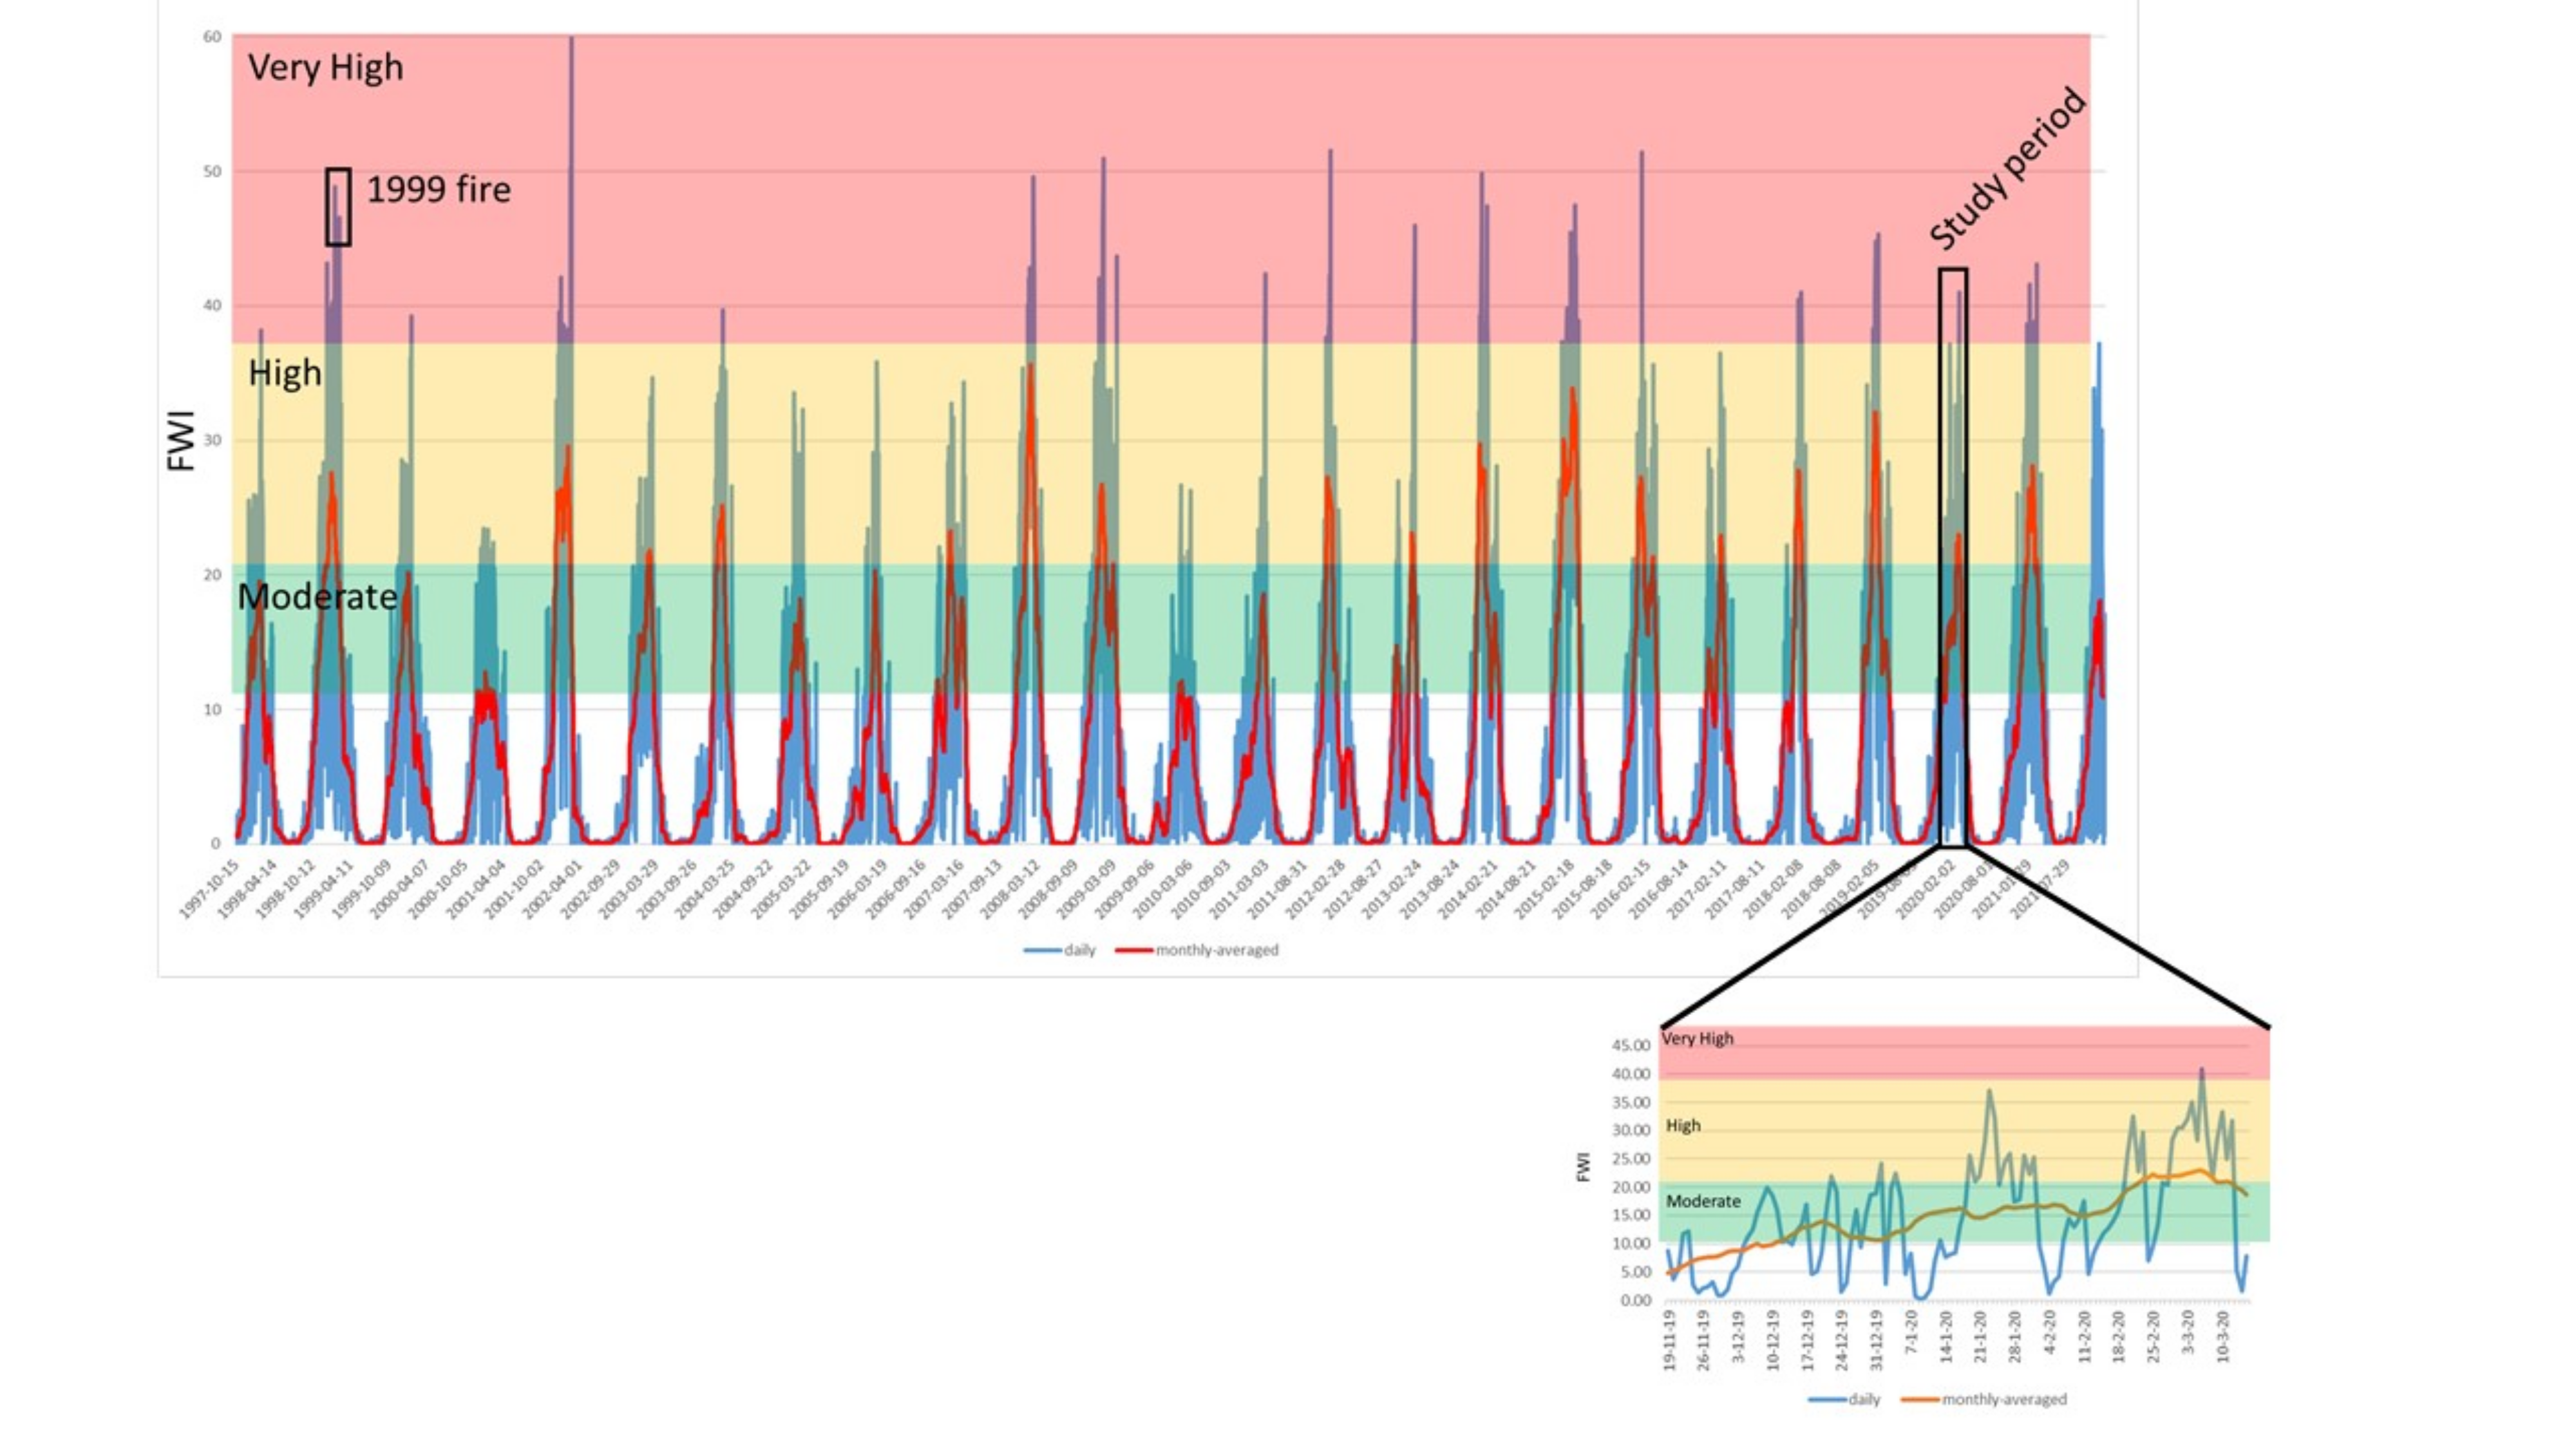
\includegraphics[width=16cm]{figuras/cap2/S01) fwi ts.png}
    \caption[FWI en el período de estudio.]{Fire Weather Index (FWI) diario (línea azul) y promedio mensual (línea roja) calculado a largo plazo (1998-2022) (arriba, izquierda) y entre el 19 de noviembre de 2019 y el 15 de marzo de 2020 (abajo, derecha) basados en el reanálisis de ERA5 del ECMWF (European Centre for Medium-Range Weather Forecasts/Copernicus Emergency Management Service; \citealt{vitolo_era5-based_2020}). Los colores de fondo indican las clases de peligro de incendio según el Sistema Europeo de Información sobre Incendios Forestales (EFFIS; \citealt{san-miguel-ayanz_comprehensive_2012}): moderado (11.2 a 21.3; verde), alto (21.3 a 38; amarillo) y muy alto (38 a 50; rojo). Los rectángulos negros señalan los valores del FWI durante el incendio de 1999 (rectángulo izquierdo) y durante el período de estudio (rectángulo derecho).}
    \label{fig:cap2-S01}
\end{figure}

\FloatBarrier

\section{Estructura de la vegetación}\label{append:veg-structure}

Evaluamos la composición de especies para explorar sus efectos sobre el contenido de humedad del combustible y caracterizamos la estructura del combustible para evaluar si nuestros sitios mostraban los mismos patrones descritos por \citet{paritsis_positive_2015} y \citet{tiribelli_changes_2018}, quienes analizaron tamaños de muestra y áreas de estudio más grandes. Construimos perfiles verticales de combustible utilizando el método de intersección con varilla \citet{paritsis_positive_2015, tiribelli_changes_2018}. En 30-60 puntos ubicados en cuadrículas rectangulares (con al menos 2 m entre puntos) en cada sitio, colocamos una varilla de 4 m de altura dividida en 16 segmentos de 25 cm y registramos la presencia de combustible fino (hojas o ramas finas $< 6$ mm) en un radio de 10 cm alrededor de la varilla en cada segmento, identificando las especies leñosas y si se trataba de material vivo o muerto. También medimos la profundidad de la capa de hojarasca, estimamos visualmente su cobertura (proporción) en cuadrantes de 1 m$^2$ en cada punto donde se colocó la varilla, y estimamos la cobertura del dosel a 1.5 m de altura en 30 puntos por sitio utilizando un \textit{smartphone} y la aplicación HabitApp. En general, los patrones de estructura de la vegetación coincidieron con los reportados por \citet{paritsis_positive_2015} y \citet{tiribelli_changes_2018}, aunque los sitios de matorral cerrado podrían tener una menor cantidad de combustible que el promedio estimado por \citet{tiribelli_changes_2018}.

Los combustibles finos estaban compuestos principalmente por combustible vivo (hojas y ramas finas de $< 6$ mm de diámetro), y la proporción de combustible vivo (número de segmentos con combustible sobre el número total de segmentos) fue más alta en los bosques jóvenes, seguida por los bosques maduros o los matorrales cerrados, alcanzando su mínimo en los matorrales abiertos. Considerando solo los combustibles muertos, no se observó un patrón claro de variación entre comunidades. Sin distinguir entre combustibles vivos y muertos, encontramos el mismo patrón que en los combustibles vivos, dado que estos eran los más abundantes (Fig.~\ref{fig:cap2-S02}).

\begin{figure}
    \centering
    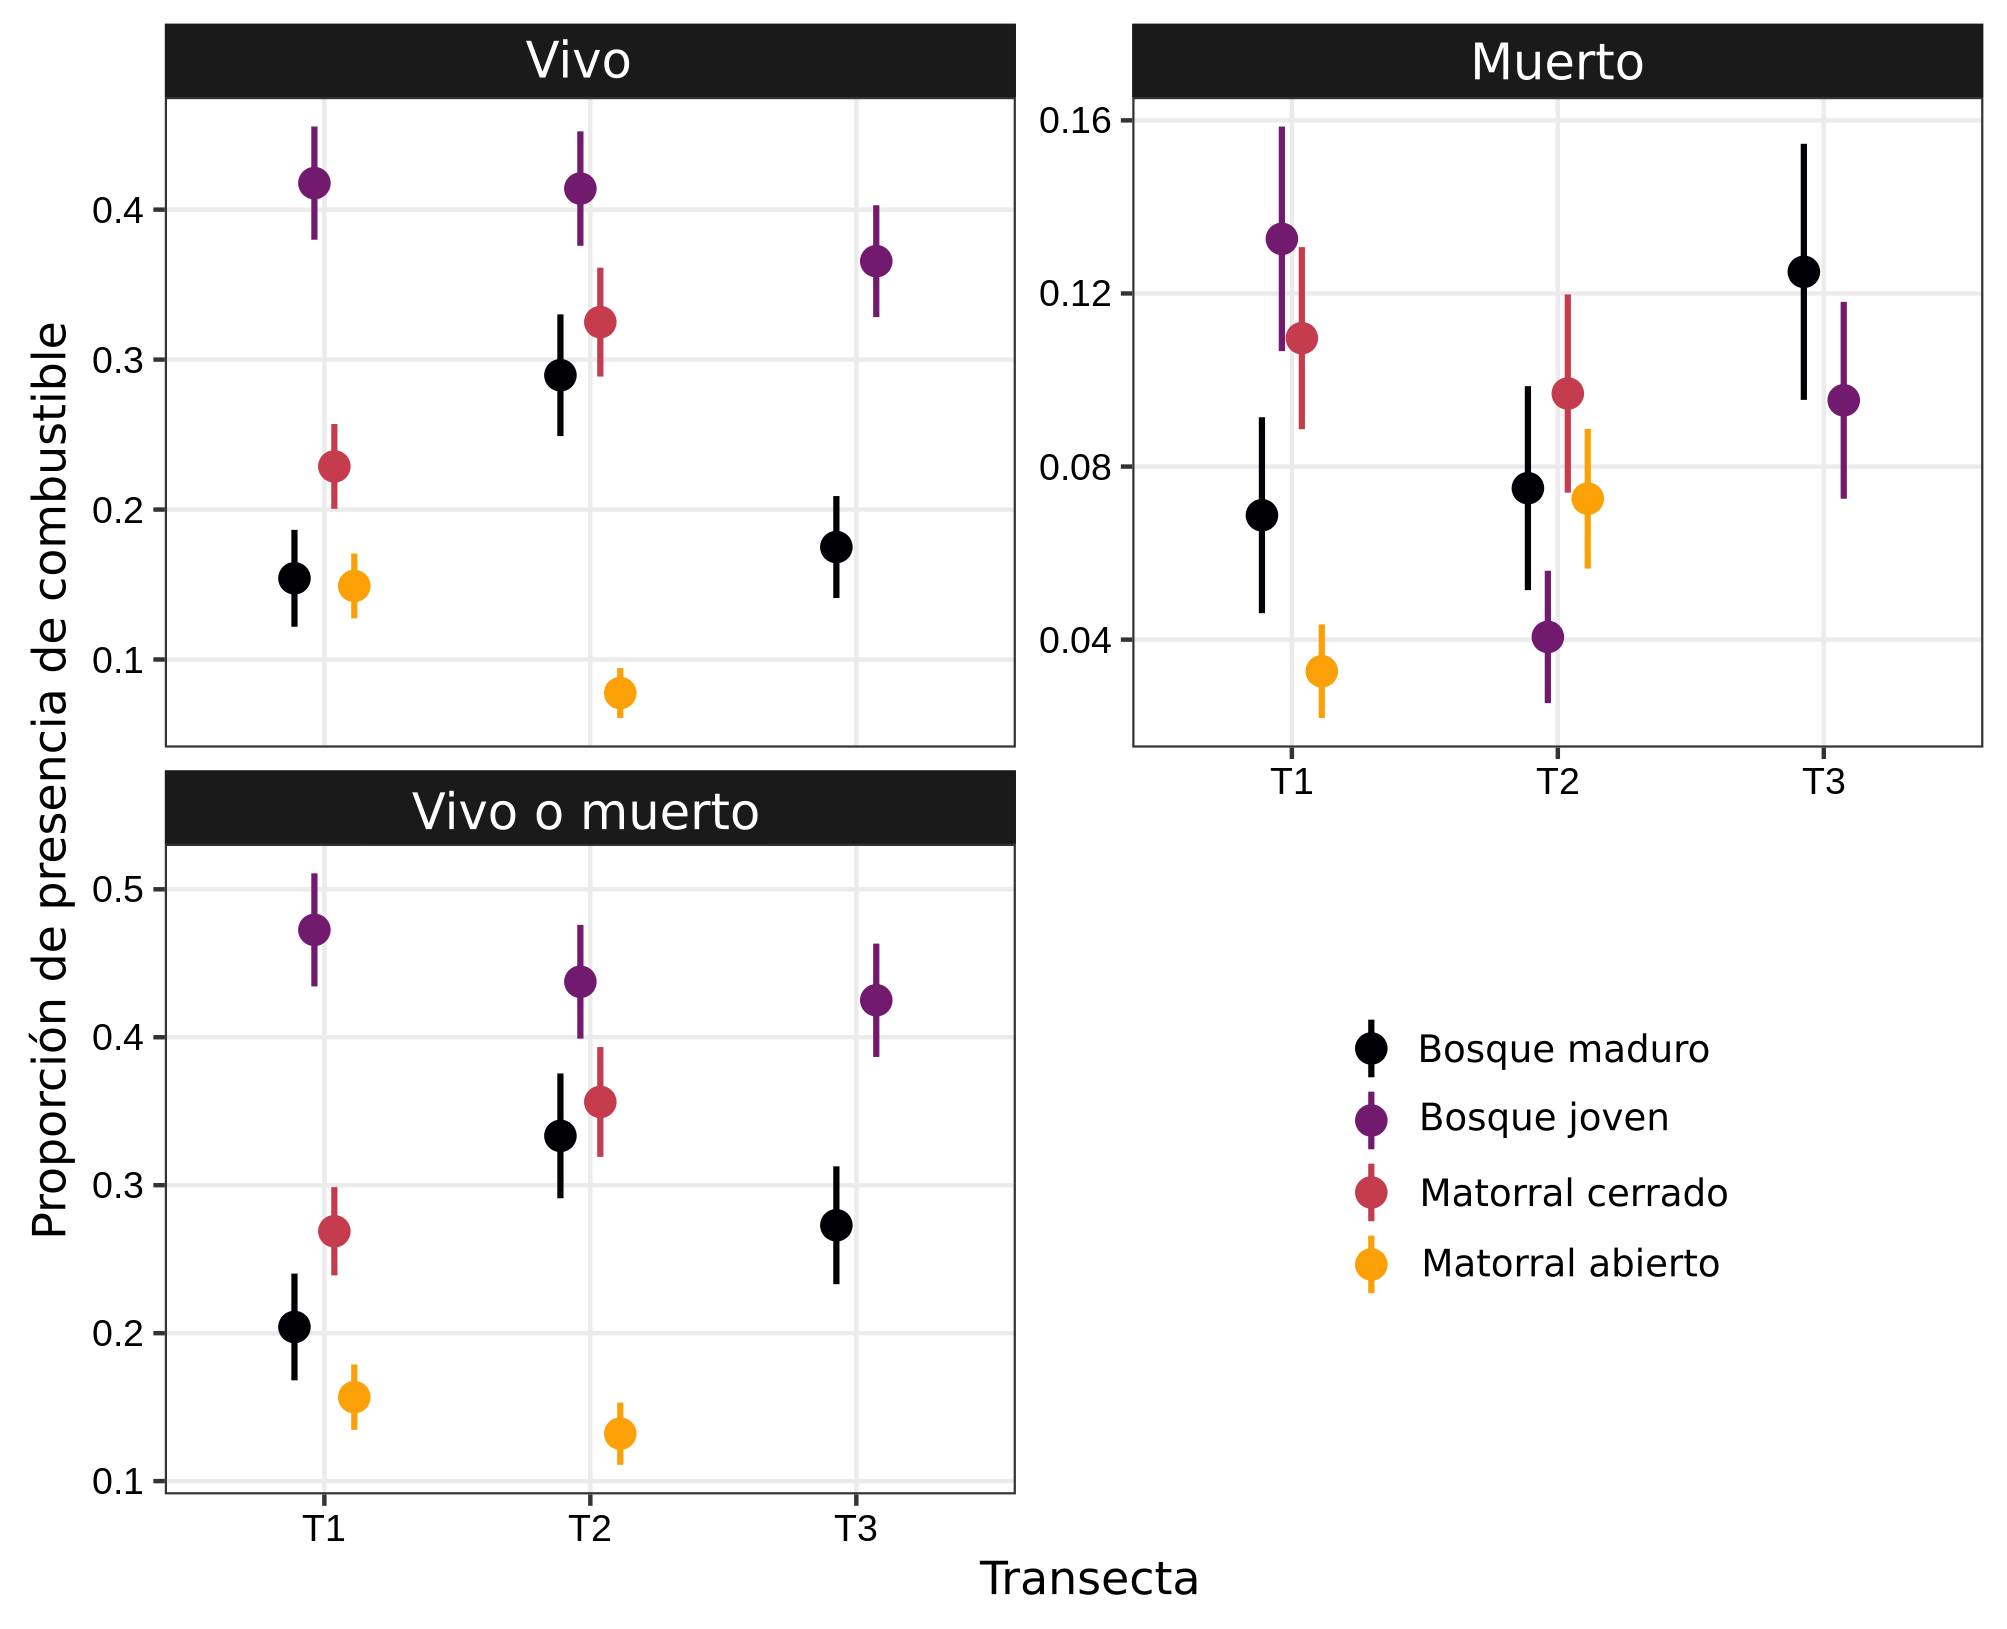
\includegraphics[width=16cm]{figuras/cap2/S02) prop fine fuel.png}
    \caption[Proporción de presencia de combustible por comunidad y transecta.]{Proporción de presencia de combustible por comunidad y transecta. Los puntos muestran la proporción de segmentos de la varilla con presencia de combustible, sin distinguir altura ni punto de muestreo. Dado que cada punto tenía 16 segmentos (varilla de 4 m, 25 cm por segmento), un sitio con 30 puntos tendría 30 $\times$ 16 = 480 segmentos. Las barras muestran $\pm 2$ desvíos estándar para las proporciones, calculadas según \citet[página 17]{GelmanHill2006}.}
    \label{fig:cap2-S02}
\end{figure}

Para analizar la continuidad vertical del combustible, ajustamos un Modelo Aditivo Generalizado (GAM) Binomial en el que la probabilidad de presencia de combustible varió como una función no lineal suave de la altura, la cual varió entre tipos de combustible (vivo, muerto y vivo o muerto), transectas y comunidades. Utilizamos splines cúbicas con 11 funciones base y ajustamos el modelo con el paquete de R \texttt{mgcv} \citep{wood_generalized_2017}. Los perfiles verticales de combustible muestran que los bosques jóvenes presentan la mayor probabilidad de presencia de combustible en todas las alturas, seguidos por los bosques maduros o los matorrales cerrados. Los matorrales abiertos muestran la menor probabilidad de presencia de combustible, excepto a baja altura, donde es alta debido a la presencia de la capa de pastos. Los matorrales cerrados presentan una menor probabilidad de presencia de combustible a mayor altura (4 m) porque la altura de los arbustos/árboles alcanza aproximadamente los 3 m, pero la continuidad del combustible es alta hasta esa altura (Fig.~\ref{fig:cap2-S03}).

\begin{figure}
    \centering
    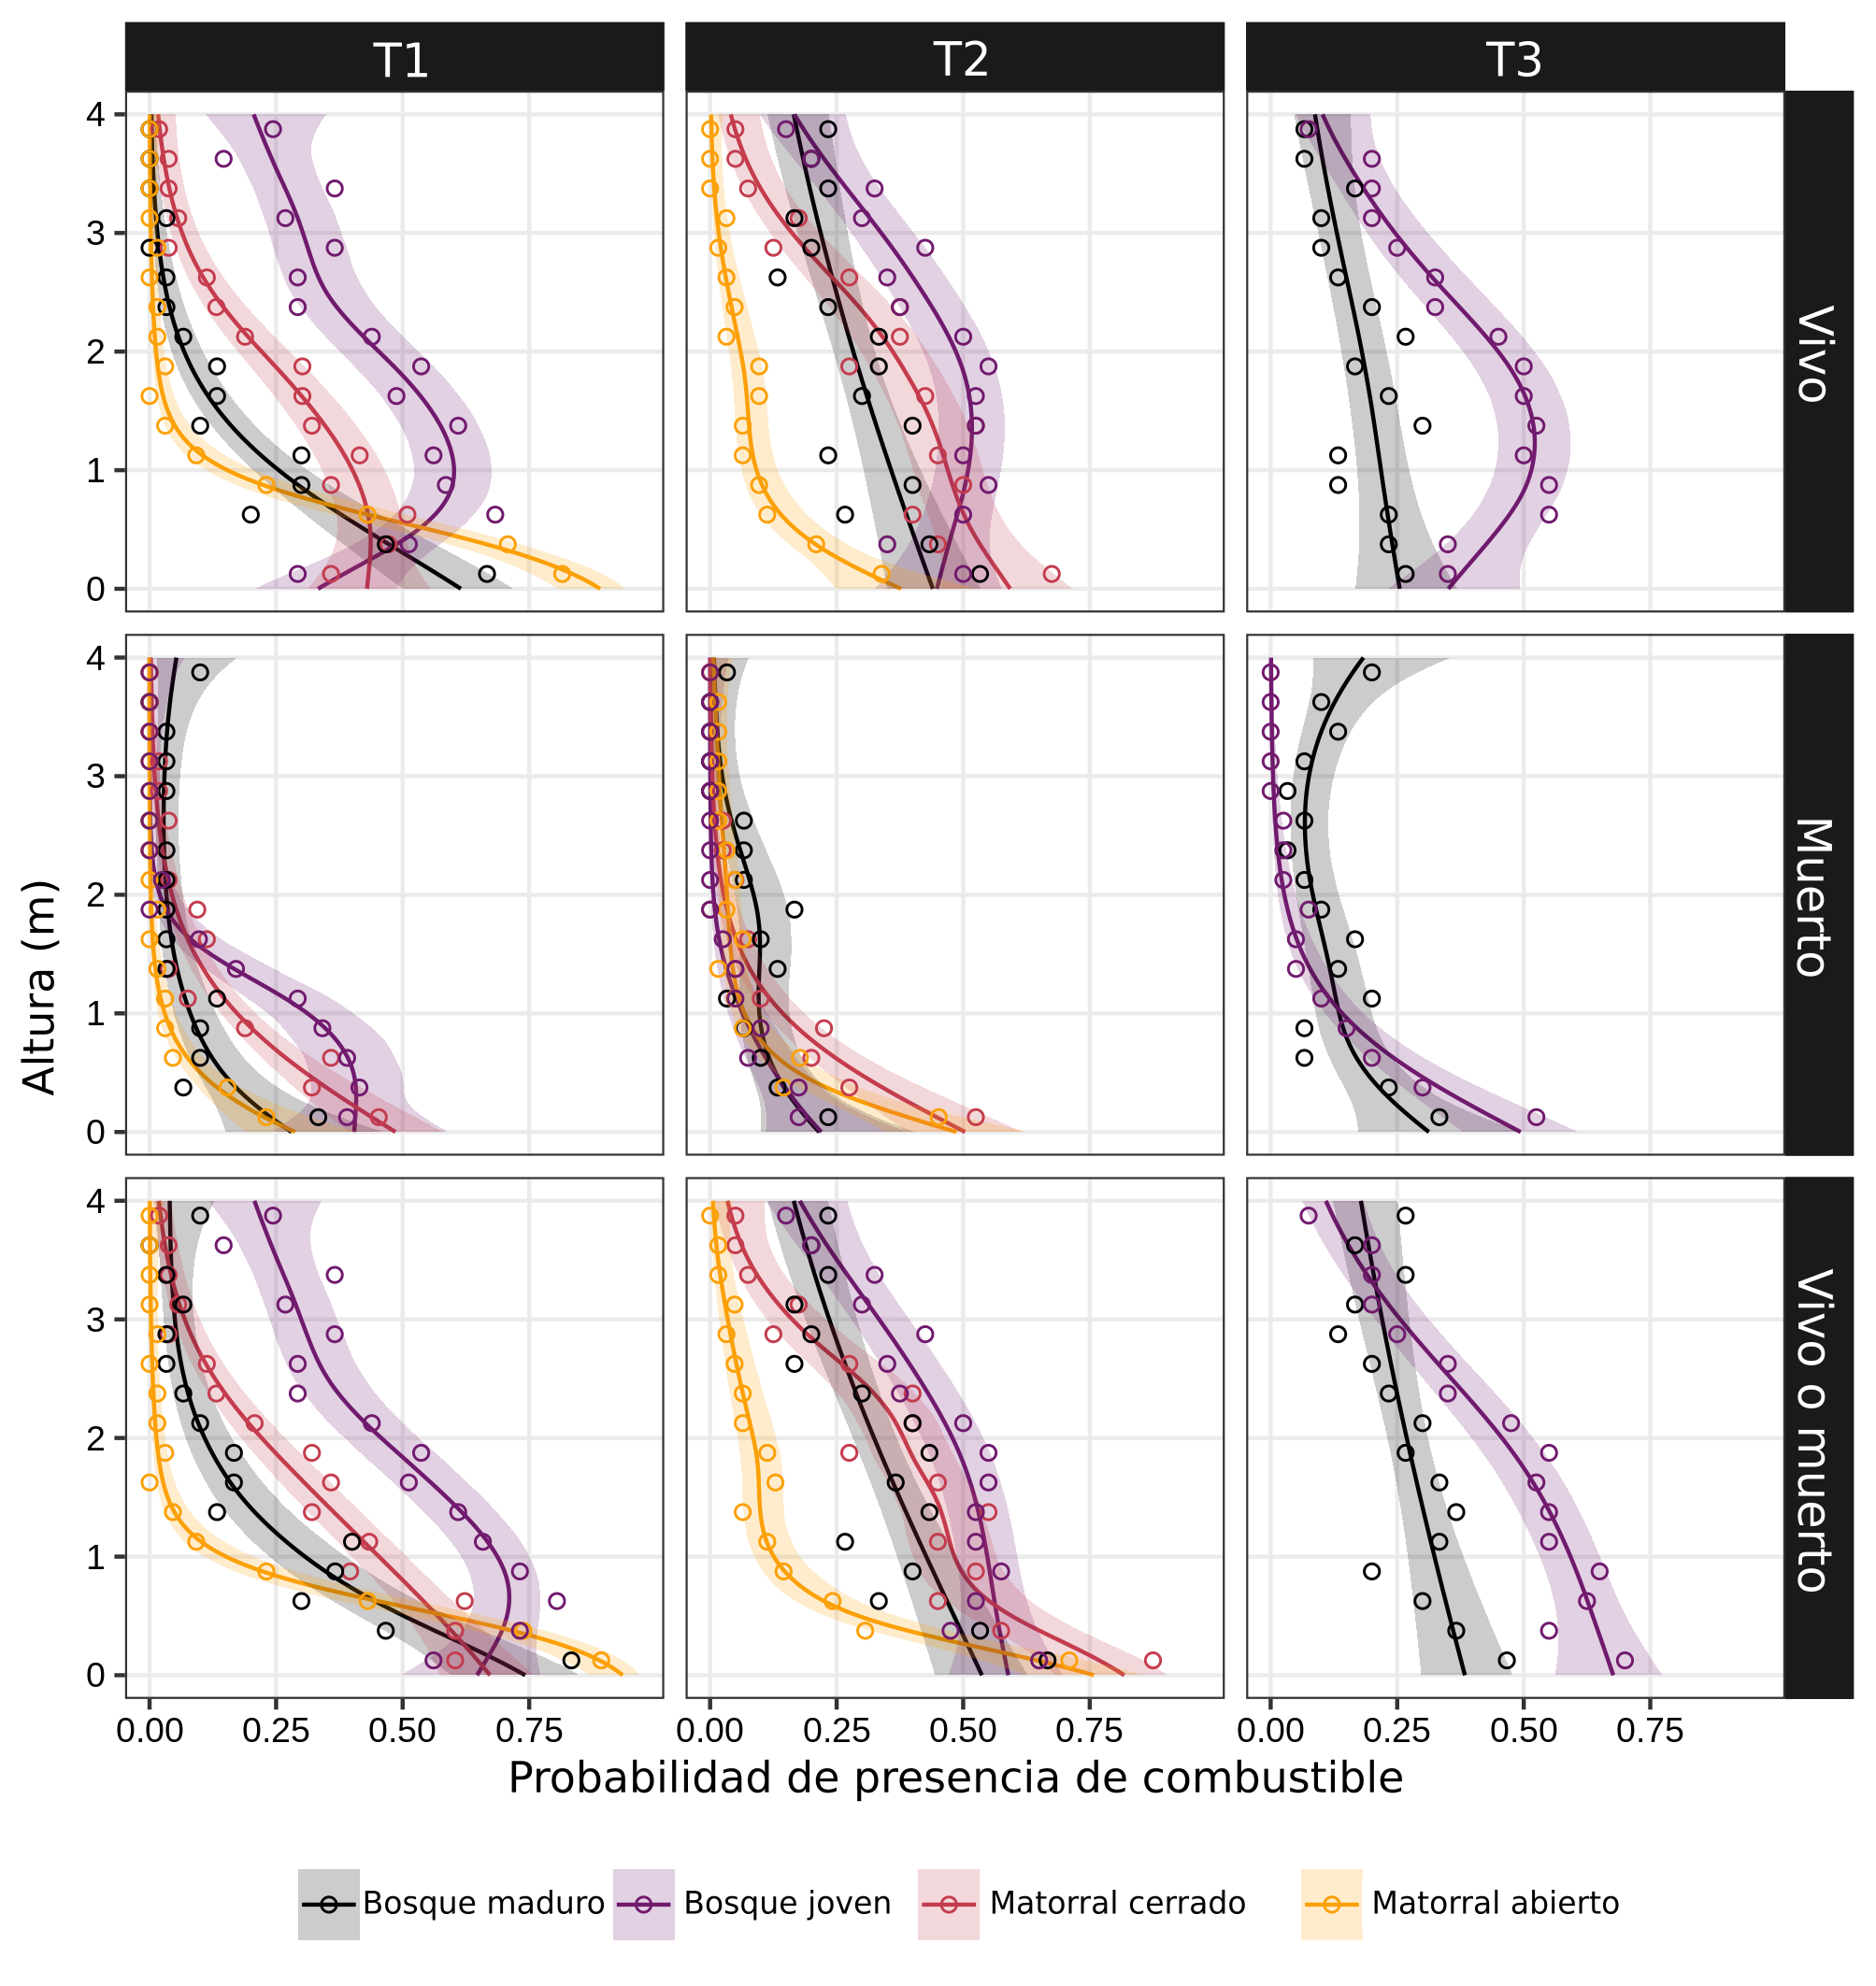
\includegraphics[width=16cm]{figuras/cap2/S03) fine fuel profile.png}
    \caption[Perfil vertical de combustible.]{Probabilidad de presencia de combustible (líneas) o proporción observada (puntos) en función de la altura, transecta y comunidad. Las líneas muestran la predicción del GAM ajustado, y las bandas sombreadas representan los intervalos de confianza del 95 \%. La variable predictora (altura) se muestra en el eje y para destacar que estos son perfiles verticales de combustible. Dado nuestro método de muestreo, la probabilidad de presencia de combustible se interpreta como la probabilidad de encontrar combustible fino en un segmento de 25 cm de altura centrado en un valor específico de altura.}
    \label{fig:cap2-S03}
\end{figure}

\citet{paritsis_positive_2015} estudiaron bosques alpinos de \textit{Nothofagus pumilio} y matorrales cercanos, mientras que \citet{tiribelli_changes_2018} estudiaron bosques de \textit{Nothofagus dombeyi} y matorrales, como hicimos nosotros. Ambos estudios encontraron patrones similares en general. \citet{tiribelli_changes_2018} estimaron una mayor proporción de combustible fino en los matorrales cerrados que en los bosques jóvenes 20 años después del incendio, por lo que la diferencia opuesta que encontramos probablemente no sea un patrón general. Además, el matorral cerrado en la transecta 1 tuvo una proporción de combustible baja en comparación con las predicciones de \citet{tiribelli_changes_2018}.
Cabe destacar que, dado que consideramos un radio de 10 cm para definir la presencia de combustible con el método de intersección con varilla, es razonable encontrar valores ligeramente más altos que los reportados por \citet{tiribelli_changes_2018}.

La profundidad de la hojarasca en los bosques maduros tendió a ser menor que en los bosques jóvenes y los matorrales cerrados, pero similar o mayor que en los matorrales abiertos. La cobertura de hojarasca fue más baja en los matorrales abiertos, mientras que las diferencias entre las demás comunidades fueron pequeñas y variables entre transectas (Fig.~\ref{fig:cap2-S04}).

\begin{figure}
    \centering
    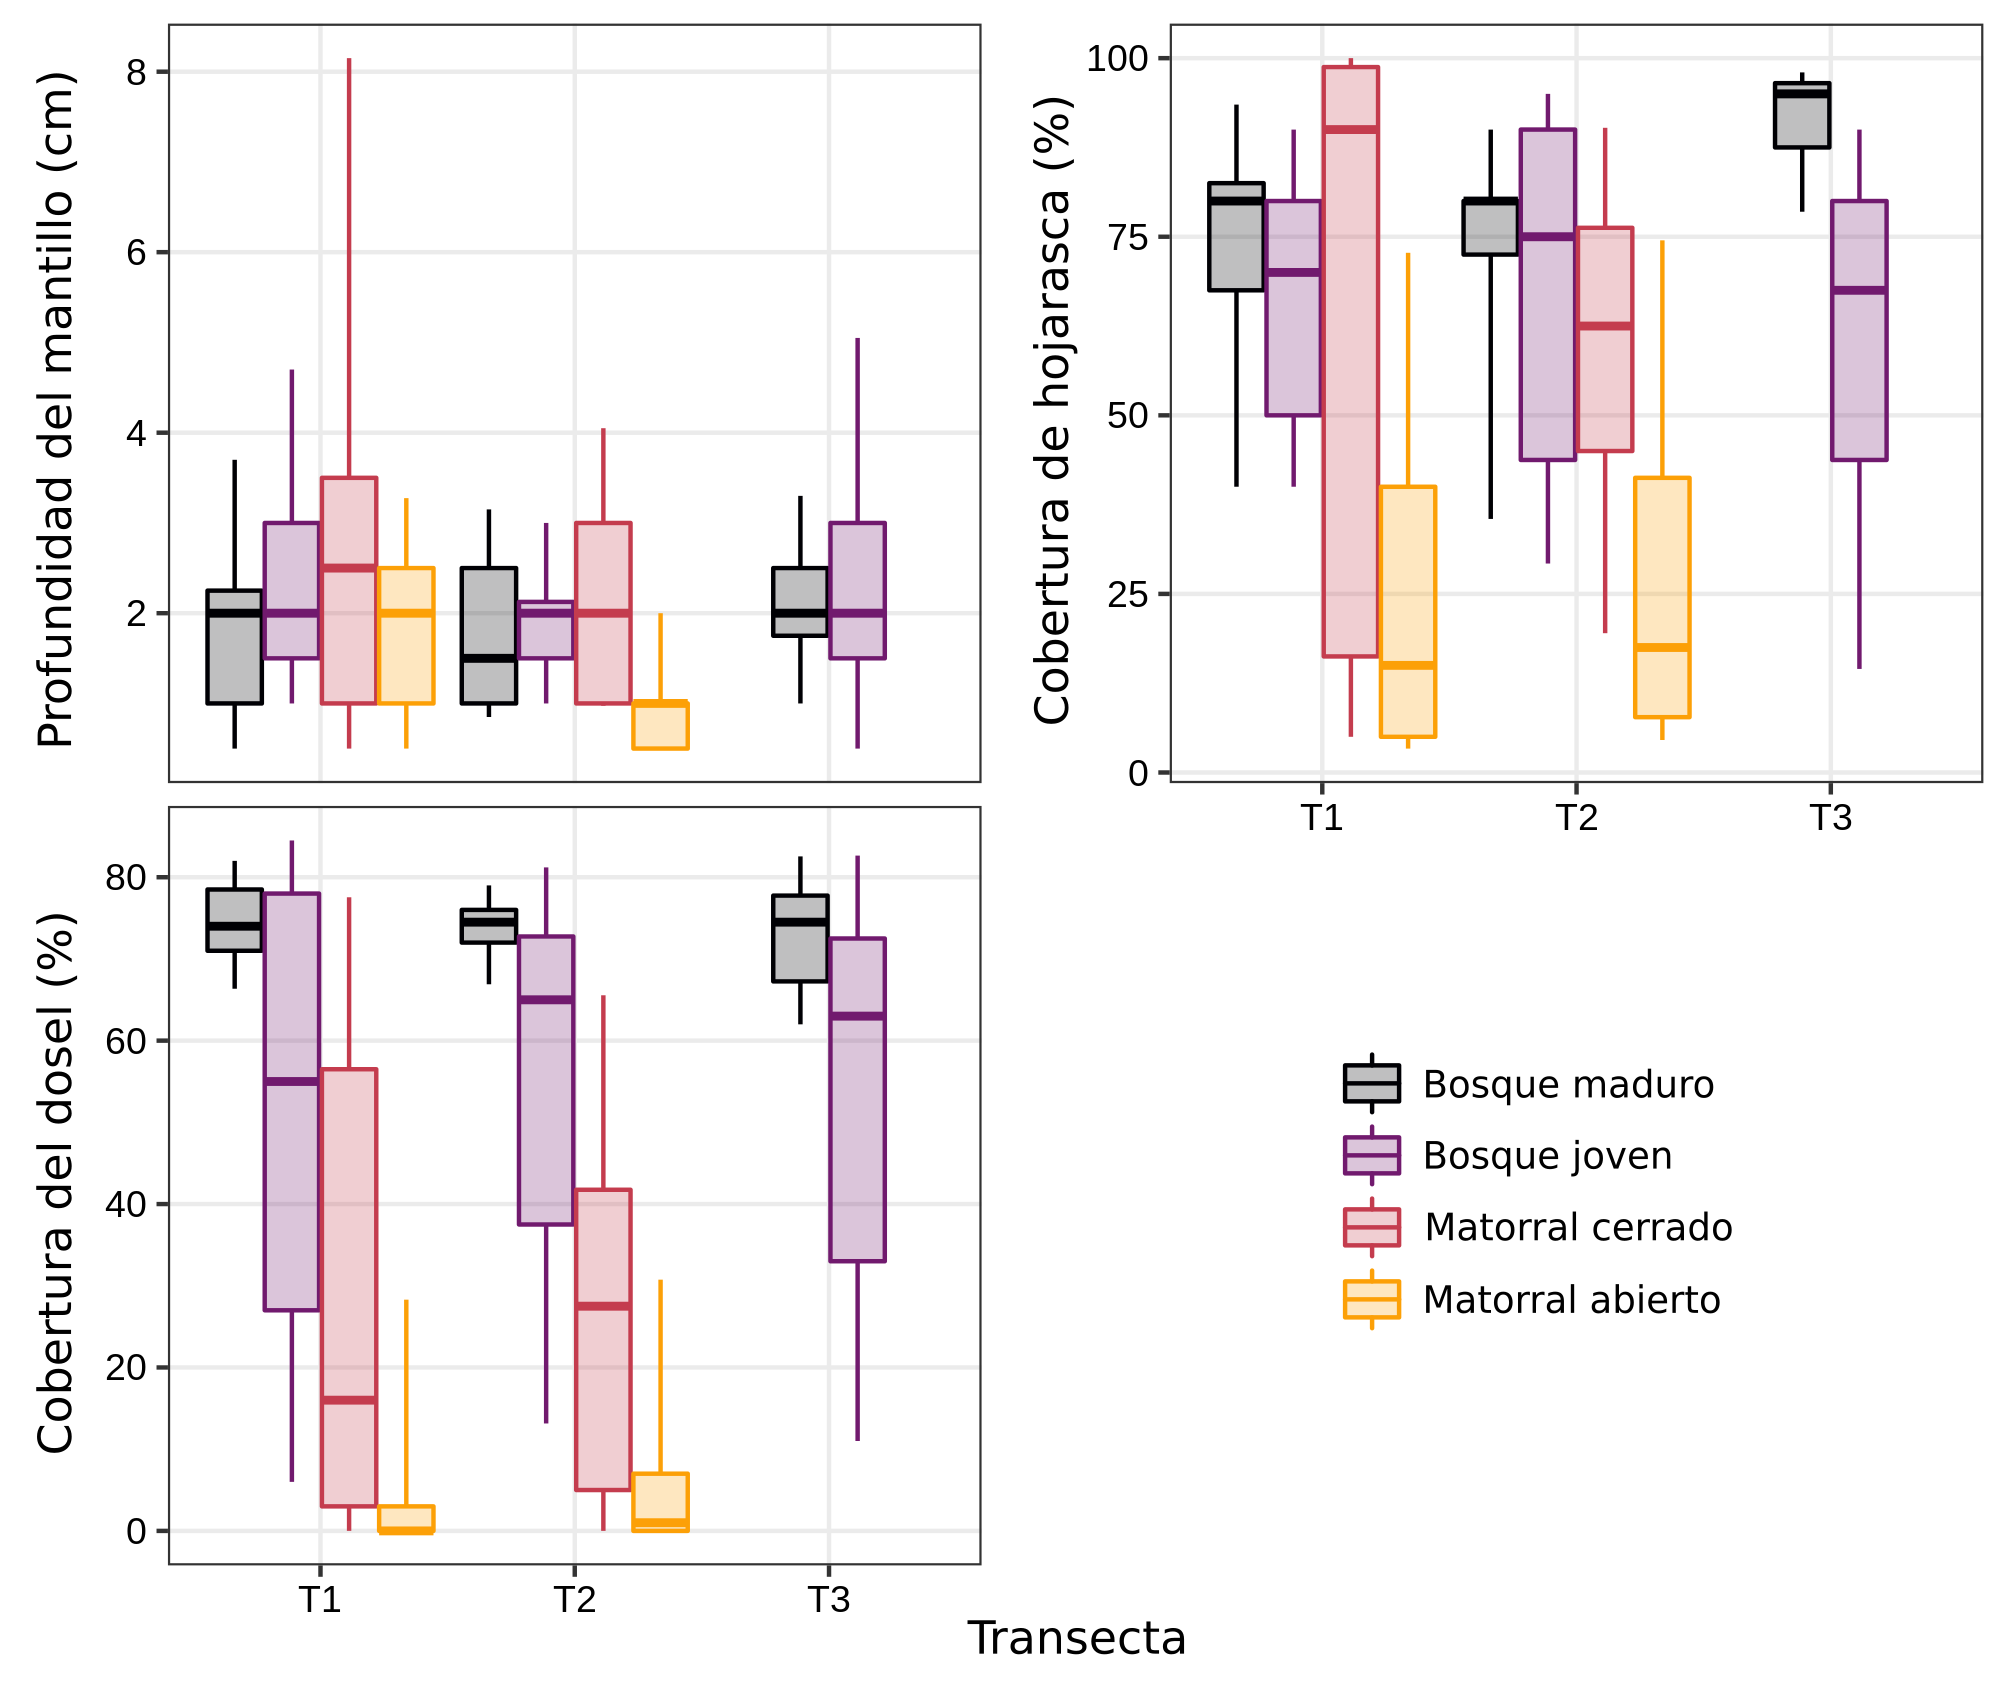
\includegraphics[width=16cm]{figuras/cap2/S04) fuel structure others.png}
    \caption[Profundidad y cobertura del mantillo y cobertura del dosel.]{Diagramas de caja para la profundidad de la hojarasca, la cobertura de la hojarasca y la cobertura del dosel por encima de 1.5 m de altura, agrupados por comunidad y transecta (percentiles 5 \%, 25 \%, 50 \%, 75 \% y 95 \%).}
    \label{fig:cap2-S04}
\end{figure}

La cobertura del dosel mostró una notable variación entre comunidades. Fue más alta en los bosques maduros y más baja en los matorrales abiertos, y estas comunidades mostraron poca variabilidad. Los bosques jóvenes y los matorrales cerrados mostraron valores intermedios, siendo más altos en los bosques jóvenes, y ambas comunidades mostraron alta variabilidad. Estos patrones fueron consistentes entre transectas (Fig.~\ref{fig:cap2-S04}).

\FloatBarrier

\section{Composición de especies}\label{append:sp-comp}

\begin{table}[ht]
\centering
\caption[Abundancia relativa de especies por comunidad y transecta.]{Abundancia relativa (\%) de especies por comunidad y transecta considerando únicamente el combustible vivo. Las especies están ordenadas de mayor a menor abundancia, considerando todos los sitios en conjunto. La abundancia relativa se derivó de los datos de intersección con varilla, describiendo la vegetación hasta 4 m de altura.}
\resizebox{\textwidth}{!}{%
\begin{tabular}{l|cccc|cccc|cc}
\toprule
Transecta & \multicolumn{4}{c}{T1} & \multicolumn{4}{c}{T2} & \multicolumn{2}{c}{T3} \\
Especie/Comunidad & BM & BJ & MC & MA & BM & BJ & MC & MA & BM & BJ \\
\hline
\textit{Nothofagus dombeyi} &  12.7 & 45.4 & 0 & 0 & 36.4 & 79.1 & 19.2 & 15.4 & 9.3 & 70.4 \\
Herbáceas &  12.7 & 5.4 & 8 & 62.6 & 6 & 3.9 & 12.9 & 29.5 & 1.2 & 7.4 \\
\textit{Schinus patagonicus} &  29.1 & 8.6 & 2.2 & 3.7 & 21.2 & 3.9 & 18.8 & 26.9 & 16.3 & 3.7 \\
\textit{Chusquea culeou} &  25.3 & 3.2 & 0 & 0 & 23.2 & 0.4 & 0 & 0 & 60.5 & 14.4 \\
\textit{Mutisia spinosa} &  0 & 14.6 & 8.8 & 27.8 & 0 & 4.6 & 7.1 & 0 & 0 & 0 \\
\textit{Lomatia hirsuta} &  0 & 14.3 & 16.8 & 0 & 0 & 0 & 21 & 0 & 8.1 & 0.8 \\
\textit{Fabiana imbricata} &  0 & 0 & 19.5 & 2.7 & 0 & 0 & 14.3 & 23.1 & 0 & 0 \\
\textit{Aristotelia chilensis} &  11.4 & 7 & 0 & 0 & 6.6 & 3.9 & 0 & 0 & 0 & 1.2 \\
\textit{Nothofagus antarctica} &  0 & 0 & 19 & 0 & 0 & 0 & 2.7 & 0 & 0 & 0 \\
\textit{Maytenus boaria} &  1.3 & 0 & 7.1 & 1.6 & 0 & 0 & 0 & 1.3 & 0 & 0.8 \\
\textit{Austrocedrus chilensis} &  7.6 & 0.6 & 0 & 0 & 0 & 0 & 0 & 0 & 0 & 0 \\
\textit{Berberis microphylla} &  0 & 0 & 2.7 & 0 & 0.7 & 1.4 & 0.9 & 0 & 1.2 & 0 \\
\textit{Diostea juncea} &  0 & 0 & 4.4 & 1.6 & 0 & 0 & 0 & 0 & 0 & 0 \\
\textit{Embothrium coccineum} &  0 & 0 & 2.2 & 0 & 3.3 & 0 & 0 & 0 & 0 & 0 \\
\textit{Discaria chacaye} &  0 & 0 & 4.4 & 0 & 0 & 0.4 & 0.4 & 0 & 0 & 0 \\
\textit{Baccharis sp.} &  0 & 0 & 3.5 & 0 & 0 & 0.4 & 0 & 0 & 0 & 0 \\
\textit{Ribes magellanicum} &  0 & 1 & 0 & 0 & 0 & 1.1 & 0.4 & 0 & 0 & 1.2 \\
\textit{Gaultheria mucronata} &  0 & 0 & 0 & 0 & 0 & 1.1 & 1.3 & 1.3 & 0 & 0 \\
\textit{Maytenus chubutensis} &  0 & 0 & 0 & 0 & 0 & 0 & 0.9 & 0 & 2.3 & 0 \\
\textit{Adesmia sp.} &  0 & 0 & 0 & 0 & 0 & 0 & 0 & 2.6 & 0 & 0 \\
\textit{Berberis serratodentata} &  0 & 0 & 0 & 0 & 2 & 0 & 0 & 0 & 0 & 0 \\
\textit{Myoschilos oblongum} &  0 & 0 & 1.3 & 0 & 0 & 0 & 0 & 0 & 0 & 0 \\
\textit{Maytenus magellanica} &  0 & 0 & 0 & 0 & 0 & 0 & 0 & 0 & 1.2 & 0 \\
\textit{Rosa rubiginosa} &  0 & 0 & 0 & 0 & 0.7 & 0 & 0 & 0 & 0 & 0 \\
\bottomrule
\end{tabular}%
}
\label{tab:sp-composition}
\end{table}


\begin{figure}
    \centering
    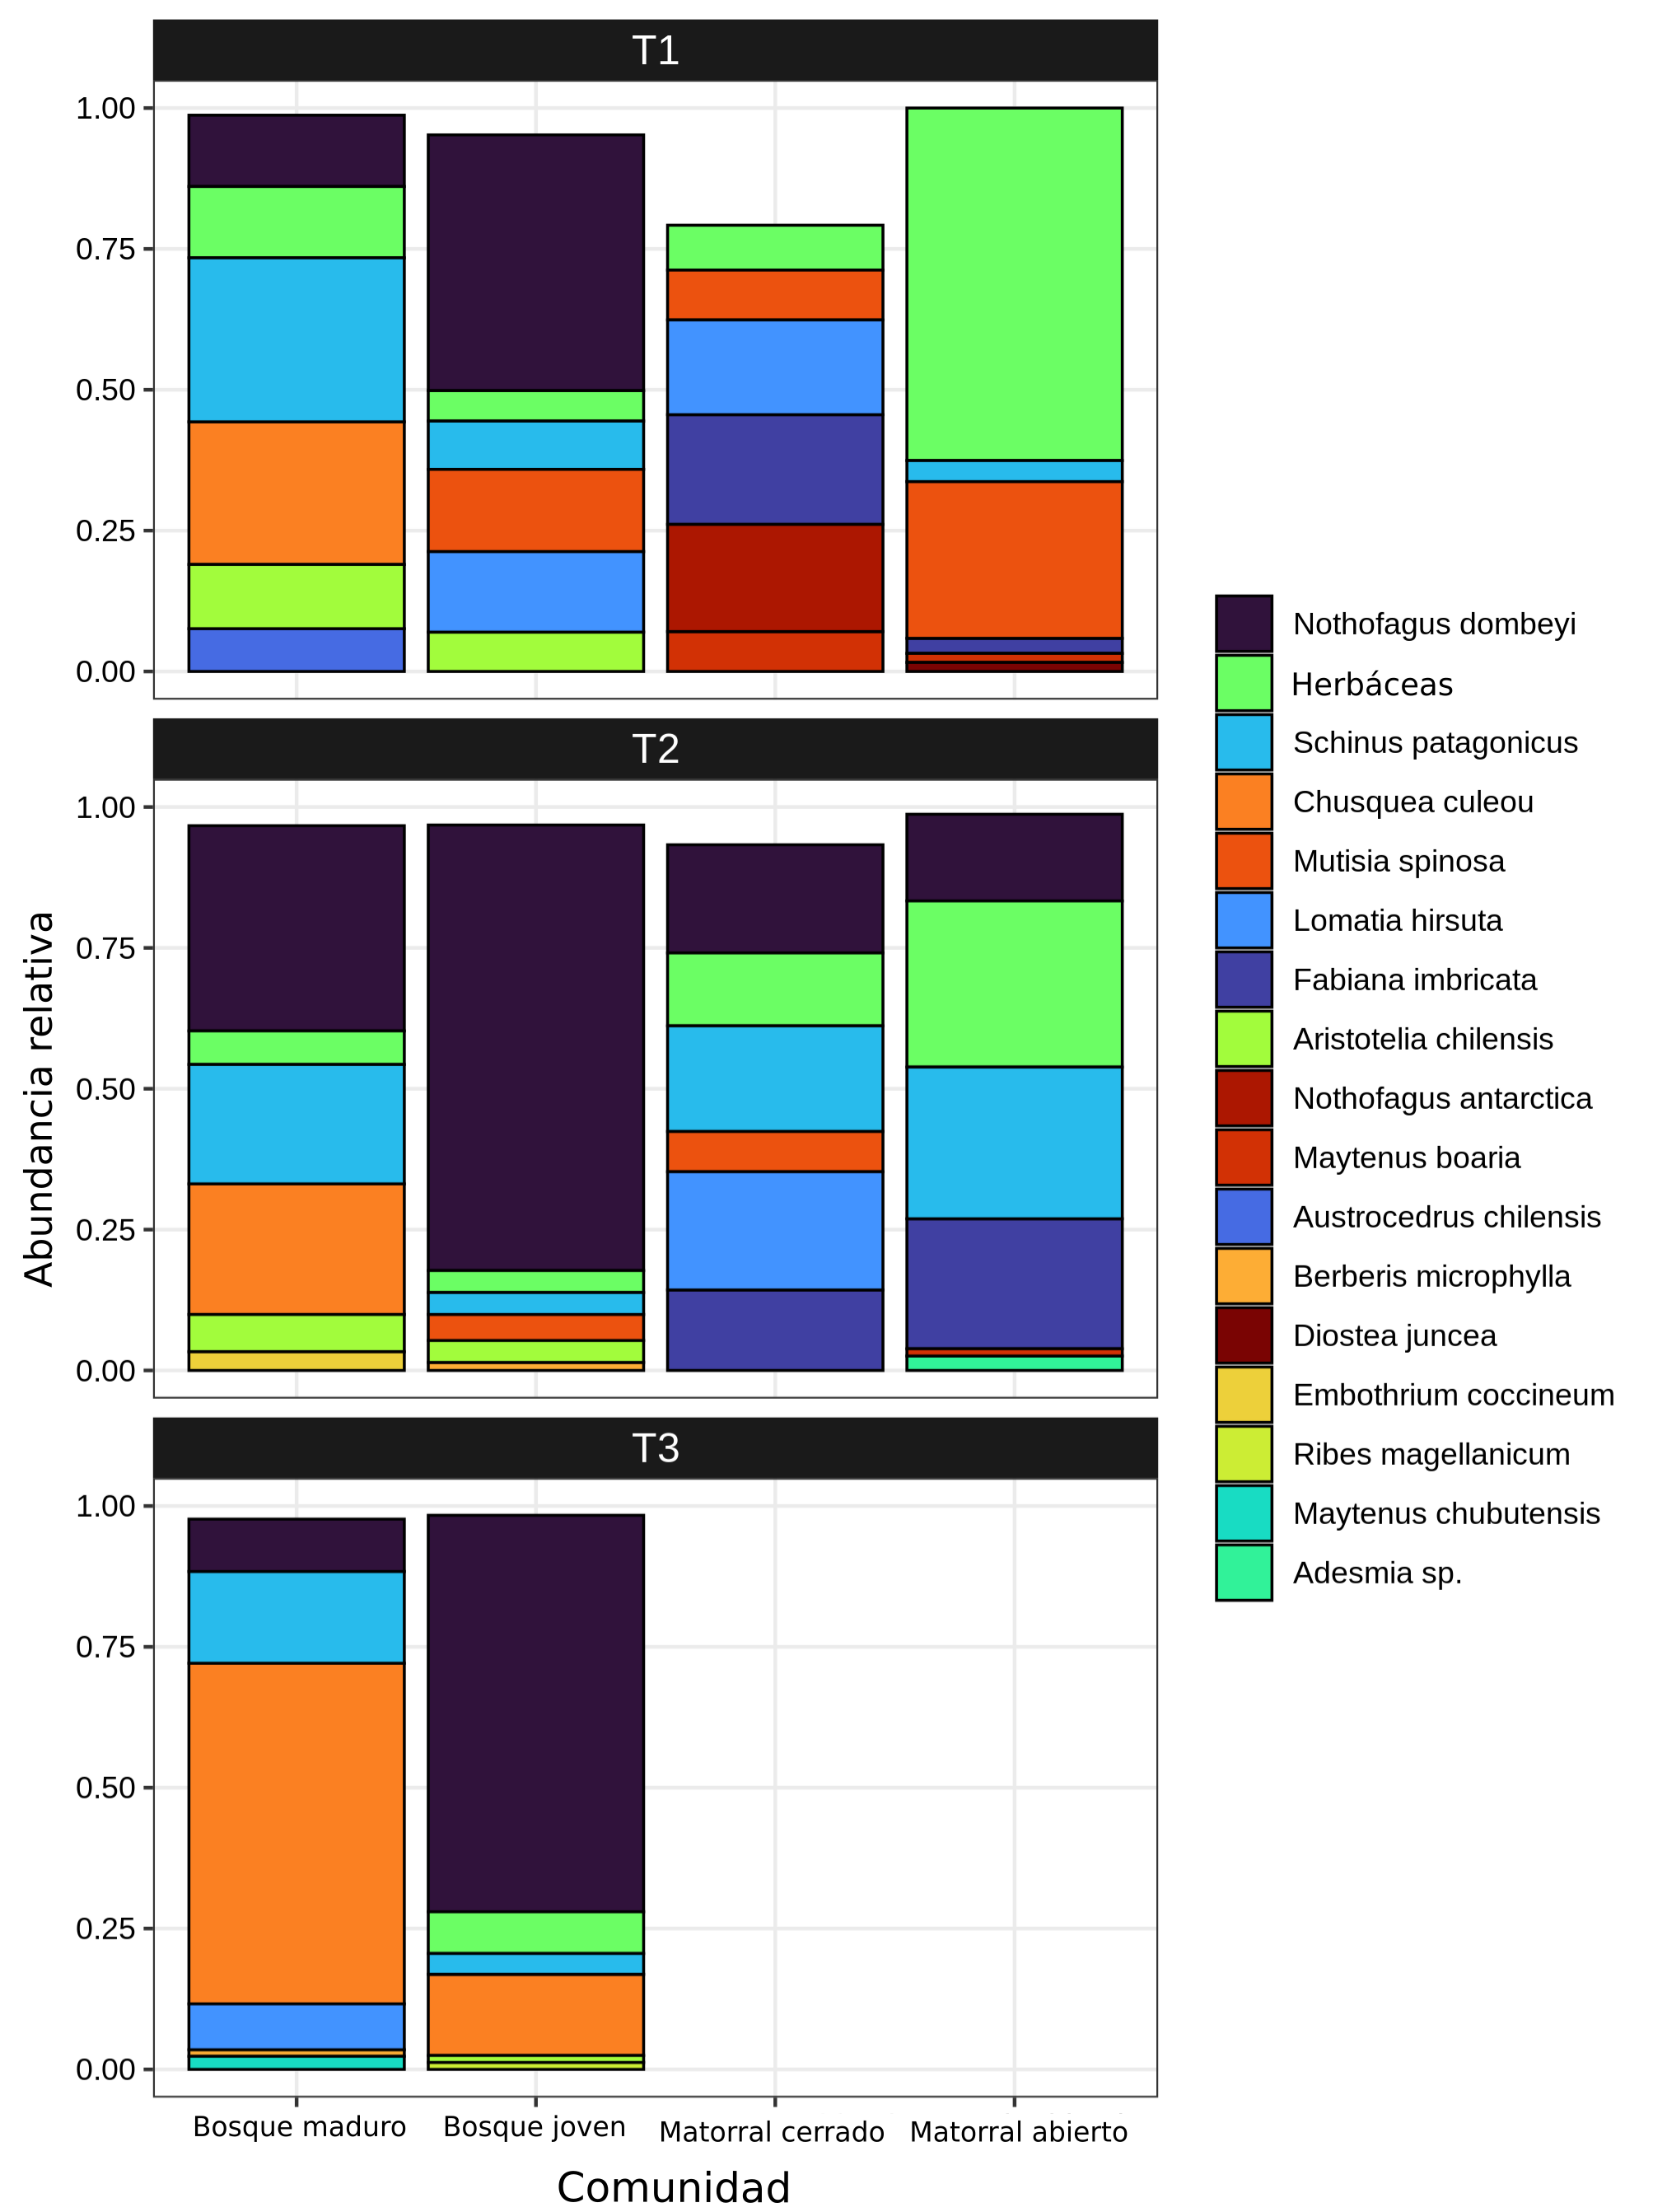
\includegraphics[width=16cm]{figuras/cap2/S05) composition.png}
    \caption[Composición de especies.]{Abundancia relativa de especies por comunidad y transecta para el combustible vivo. Solo se muestran las seis especies más abundantes en cada sitio para facilitar la visualización. La abundancia relativa se derivó de los datos de intersección con varilla, describiendo la vegetación hasta 4 m de altura.}
    \label{fig:cap2-S05}
\end{figure}

\FloatBarrier

\section{Figuras adicionales: datos y modelos de humedad del combustible}

\begin{figure}[H]
    \centering
    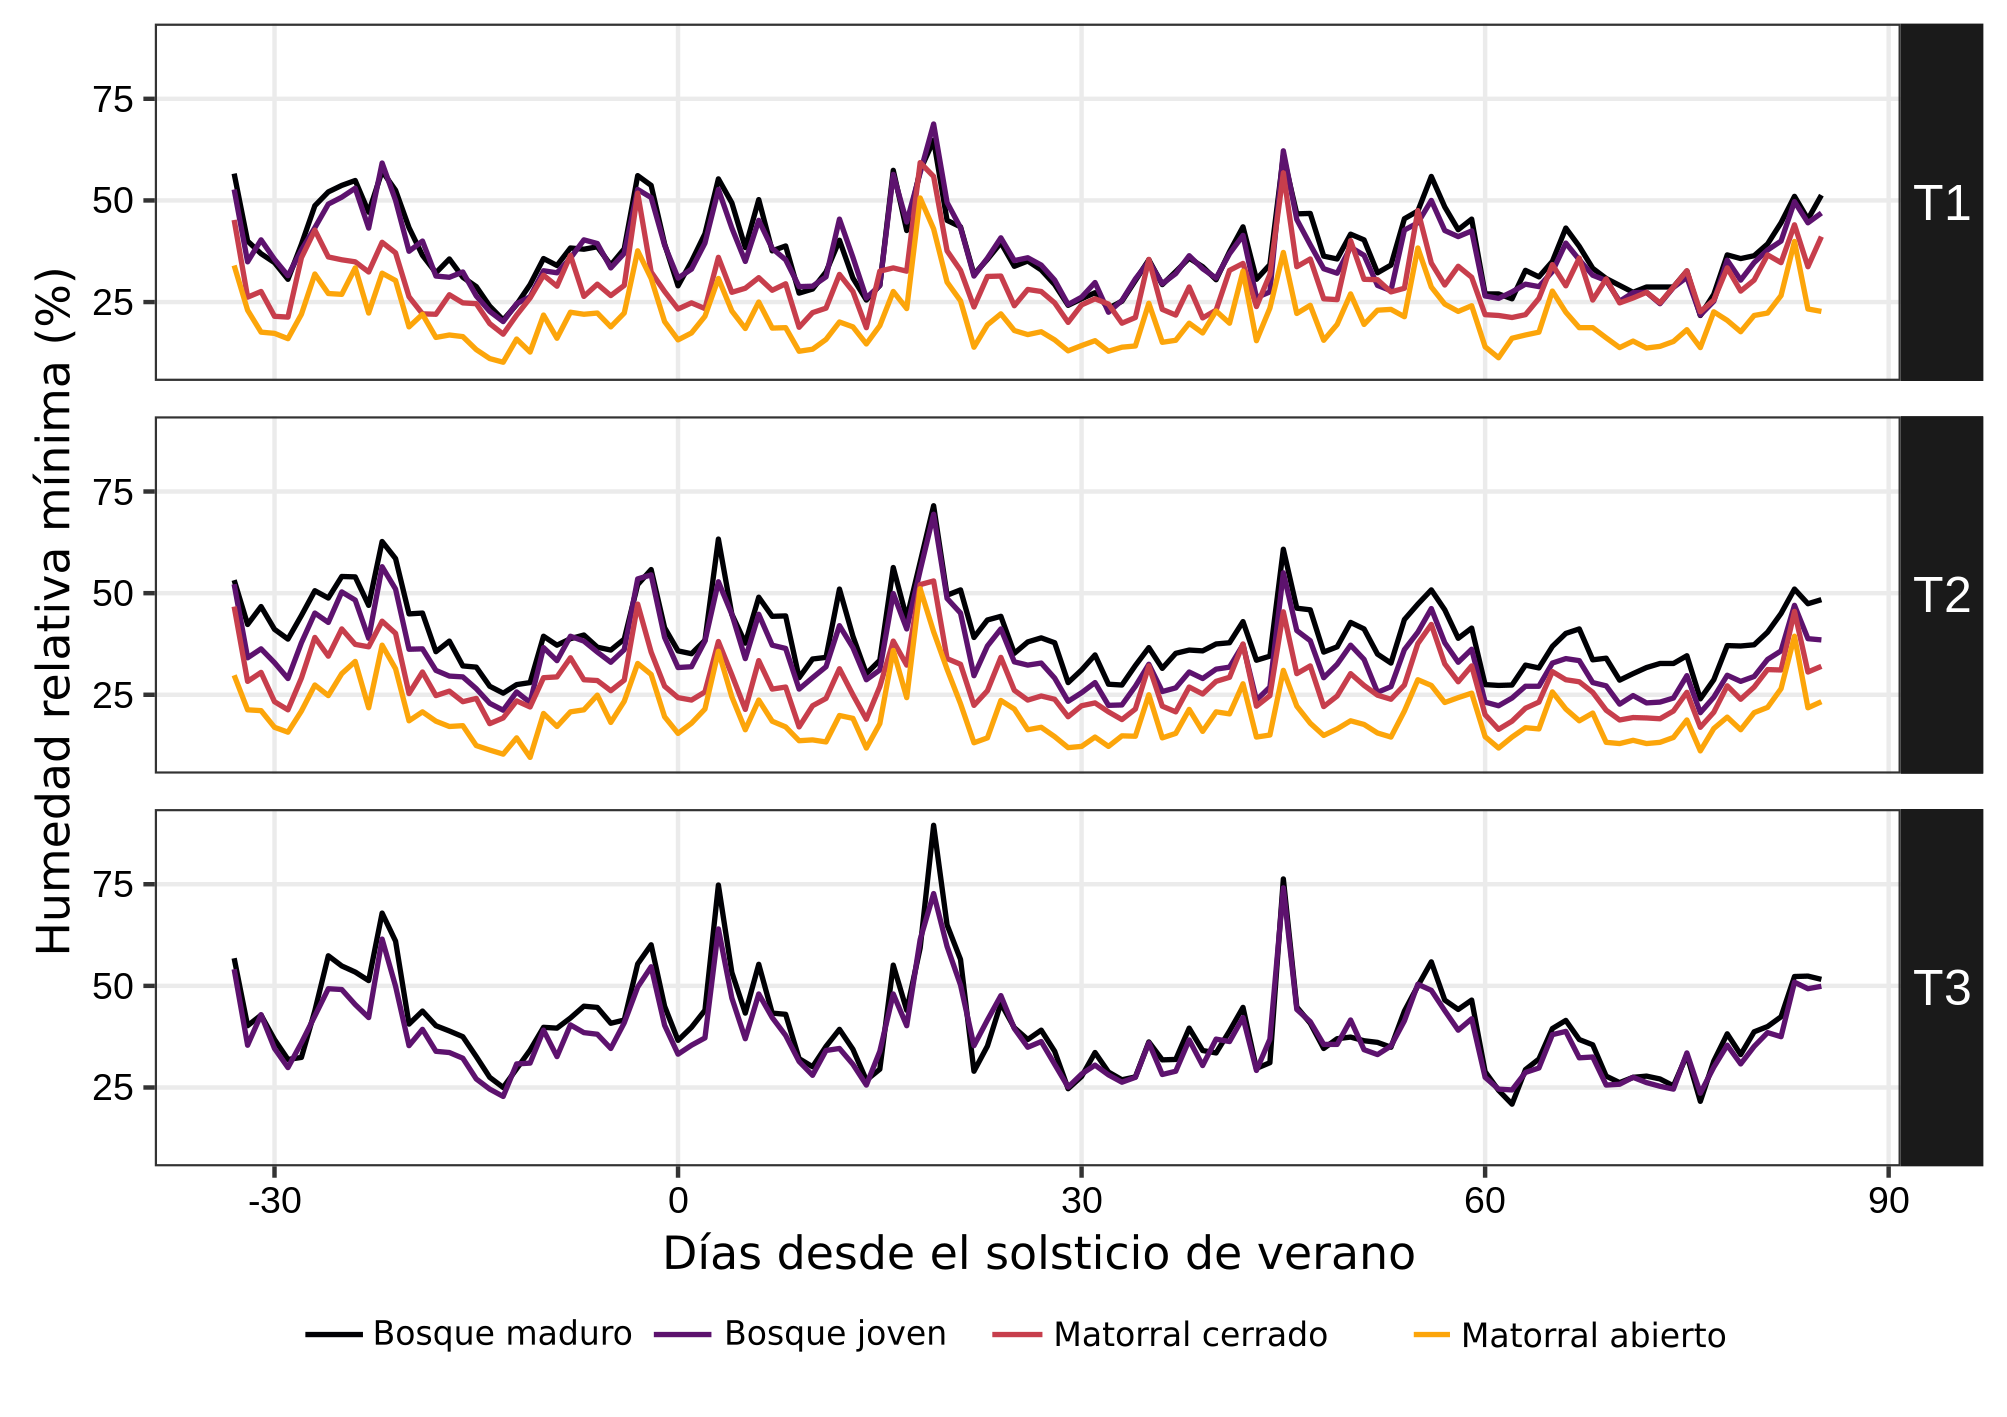
\includegraphics[width=16cm]{figuras/cap2/S06) air moisture ts.png}
    \caption[Humedad relativa del aire, series temporales.]{Humedad relativa mínima diaria (\%) a lo largo de la estación seca. El día cero corresponde al 21 de diciembre de 2019.}
    \label{fig:cap2-S06}
\end{figure}

\begin{figure}
    \centering
    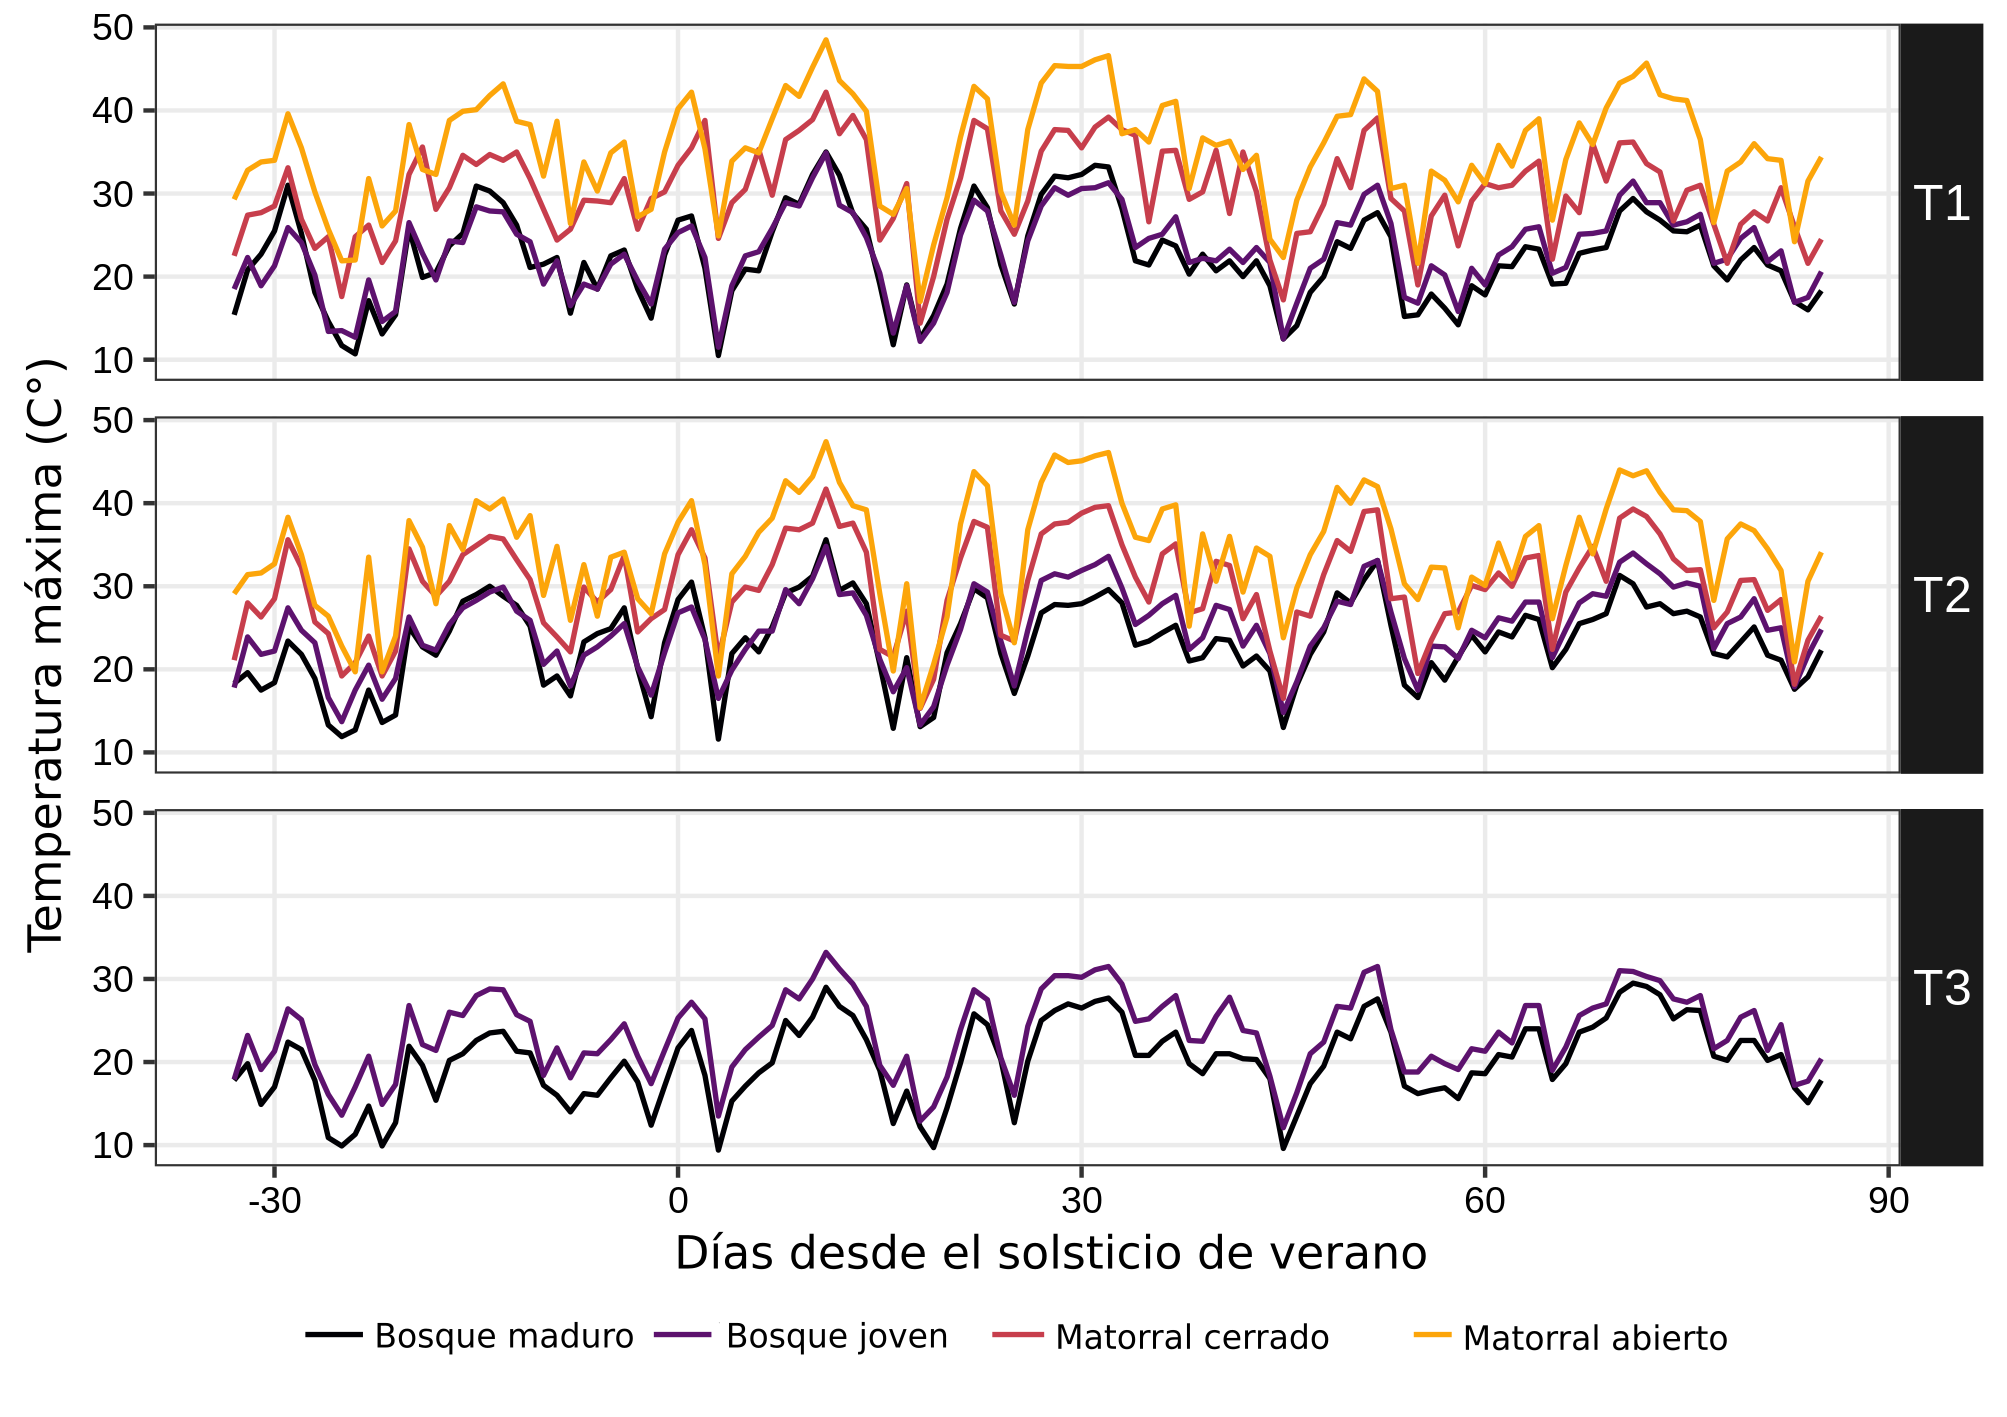
\includegraphics[width=16cm]{figuras/cap2/S07) air temperature ts.png}
    \caption[Temperatura del aire, series temporales.]{Temperatura máxima diaria (°C) a lo largo de la estación seca. El día cero corresponde al 21 de diciembre de 2019.}
    \label{fig:cap2-S07}
\end{figure}

\begin{figure}
    \centering
    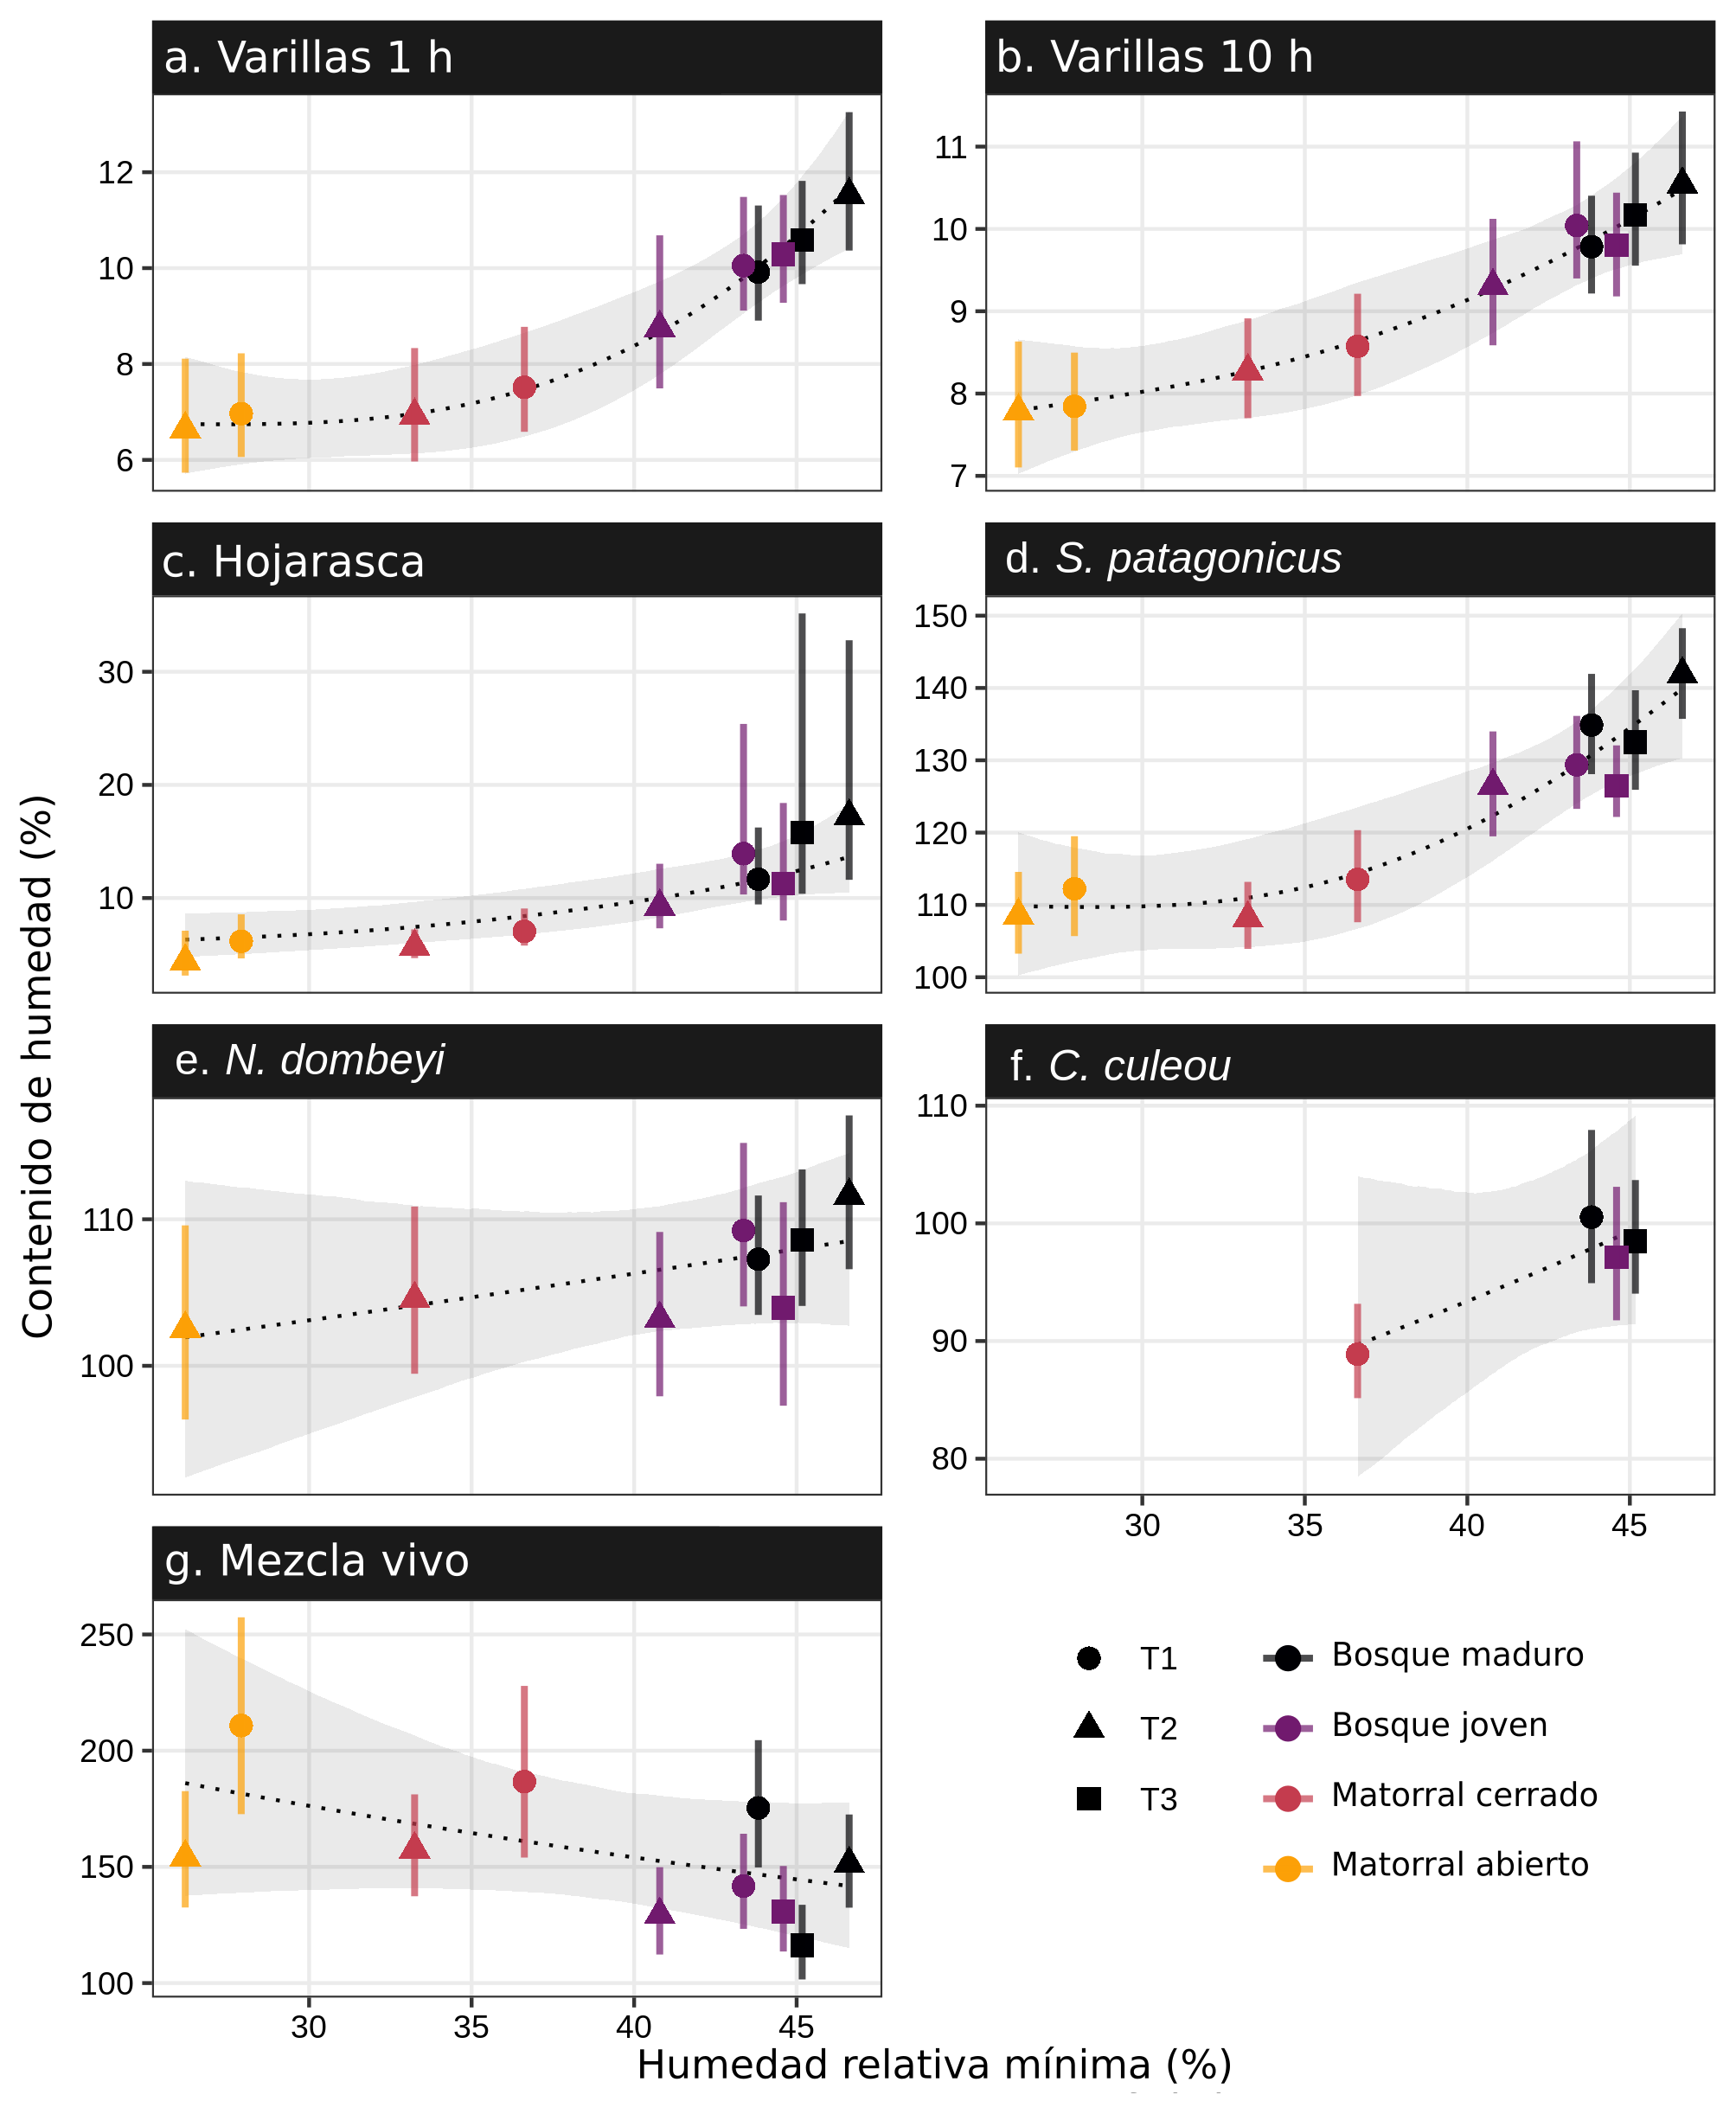
\includegraphics[width=16cm]{figuras/cap2/S08) fmc_humidity.png}
    \caption[Humedad del combustible en función de la humedad relativa del aire.]{Contenido de humedad promedio estimado en función de la humedad relativa mínima diaria promediada durante el período de estudio por sitio. Los puntos representan la media posterior para cada sitio, y las barras, los intervalos de confianza del 95\% (mismos valores que en la figura~\ref{fig:cap2-03}, panel derecho). El efecto ajustado de la temperatura se muestra con la línea discontinua (media posterior) y la banda gris (IC del 95 \%). Los modelos tuvieron la misma estructura y las mismas previas que los ajustados utilizando el DPV máximo, descritos en la Sección~\ref{cap2:humedad-methods} y en el Apéndice~\ref{append:moisture-models}.}
    \label{fig:cap2-S08}
\end{figure}

\begin{figure}
    \centering
    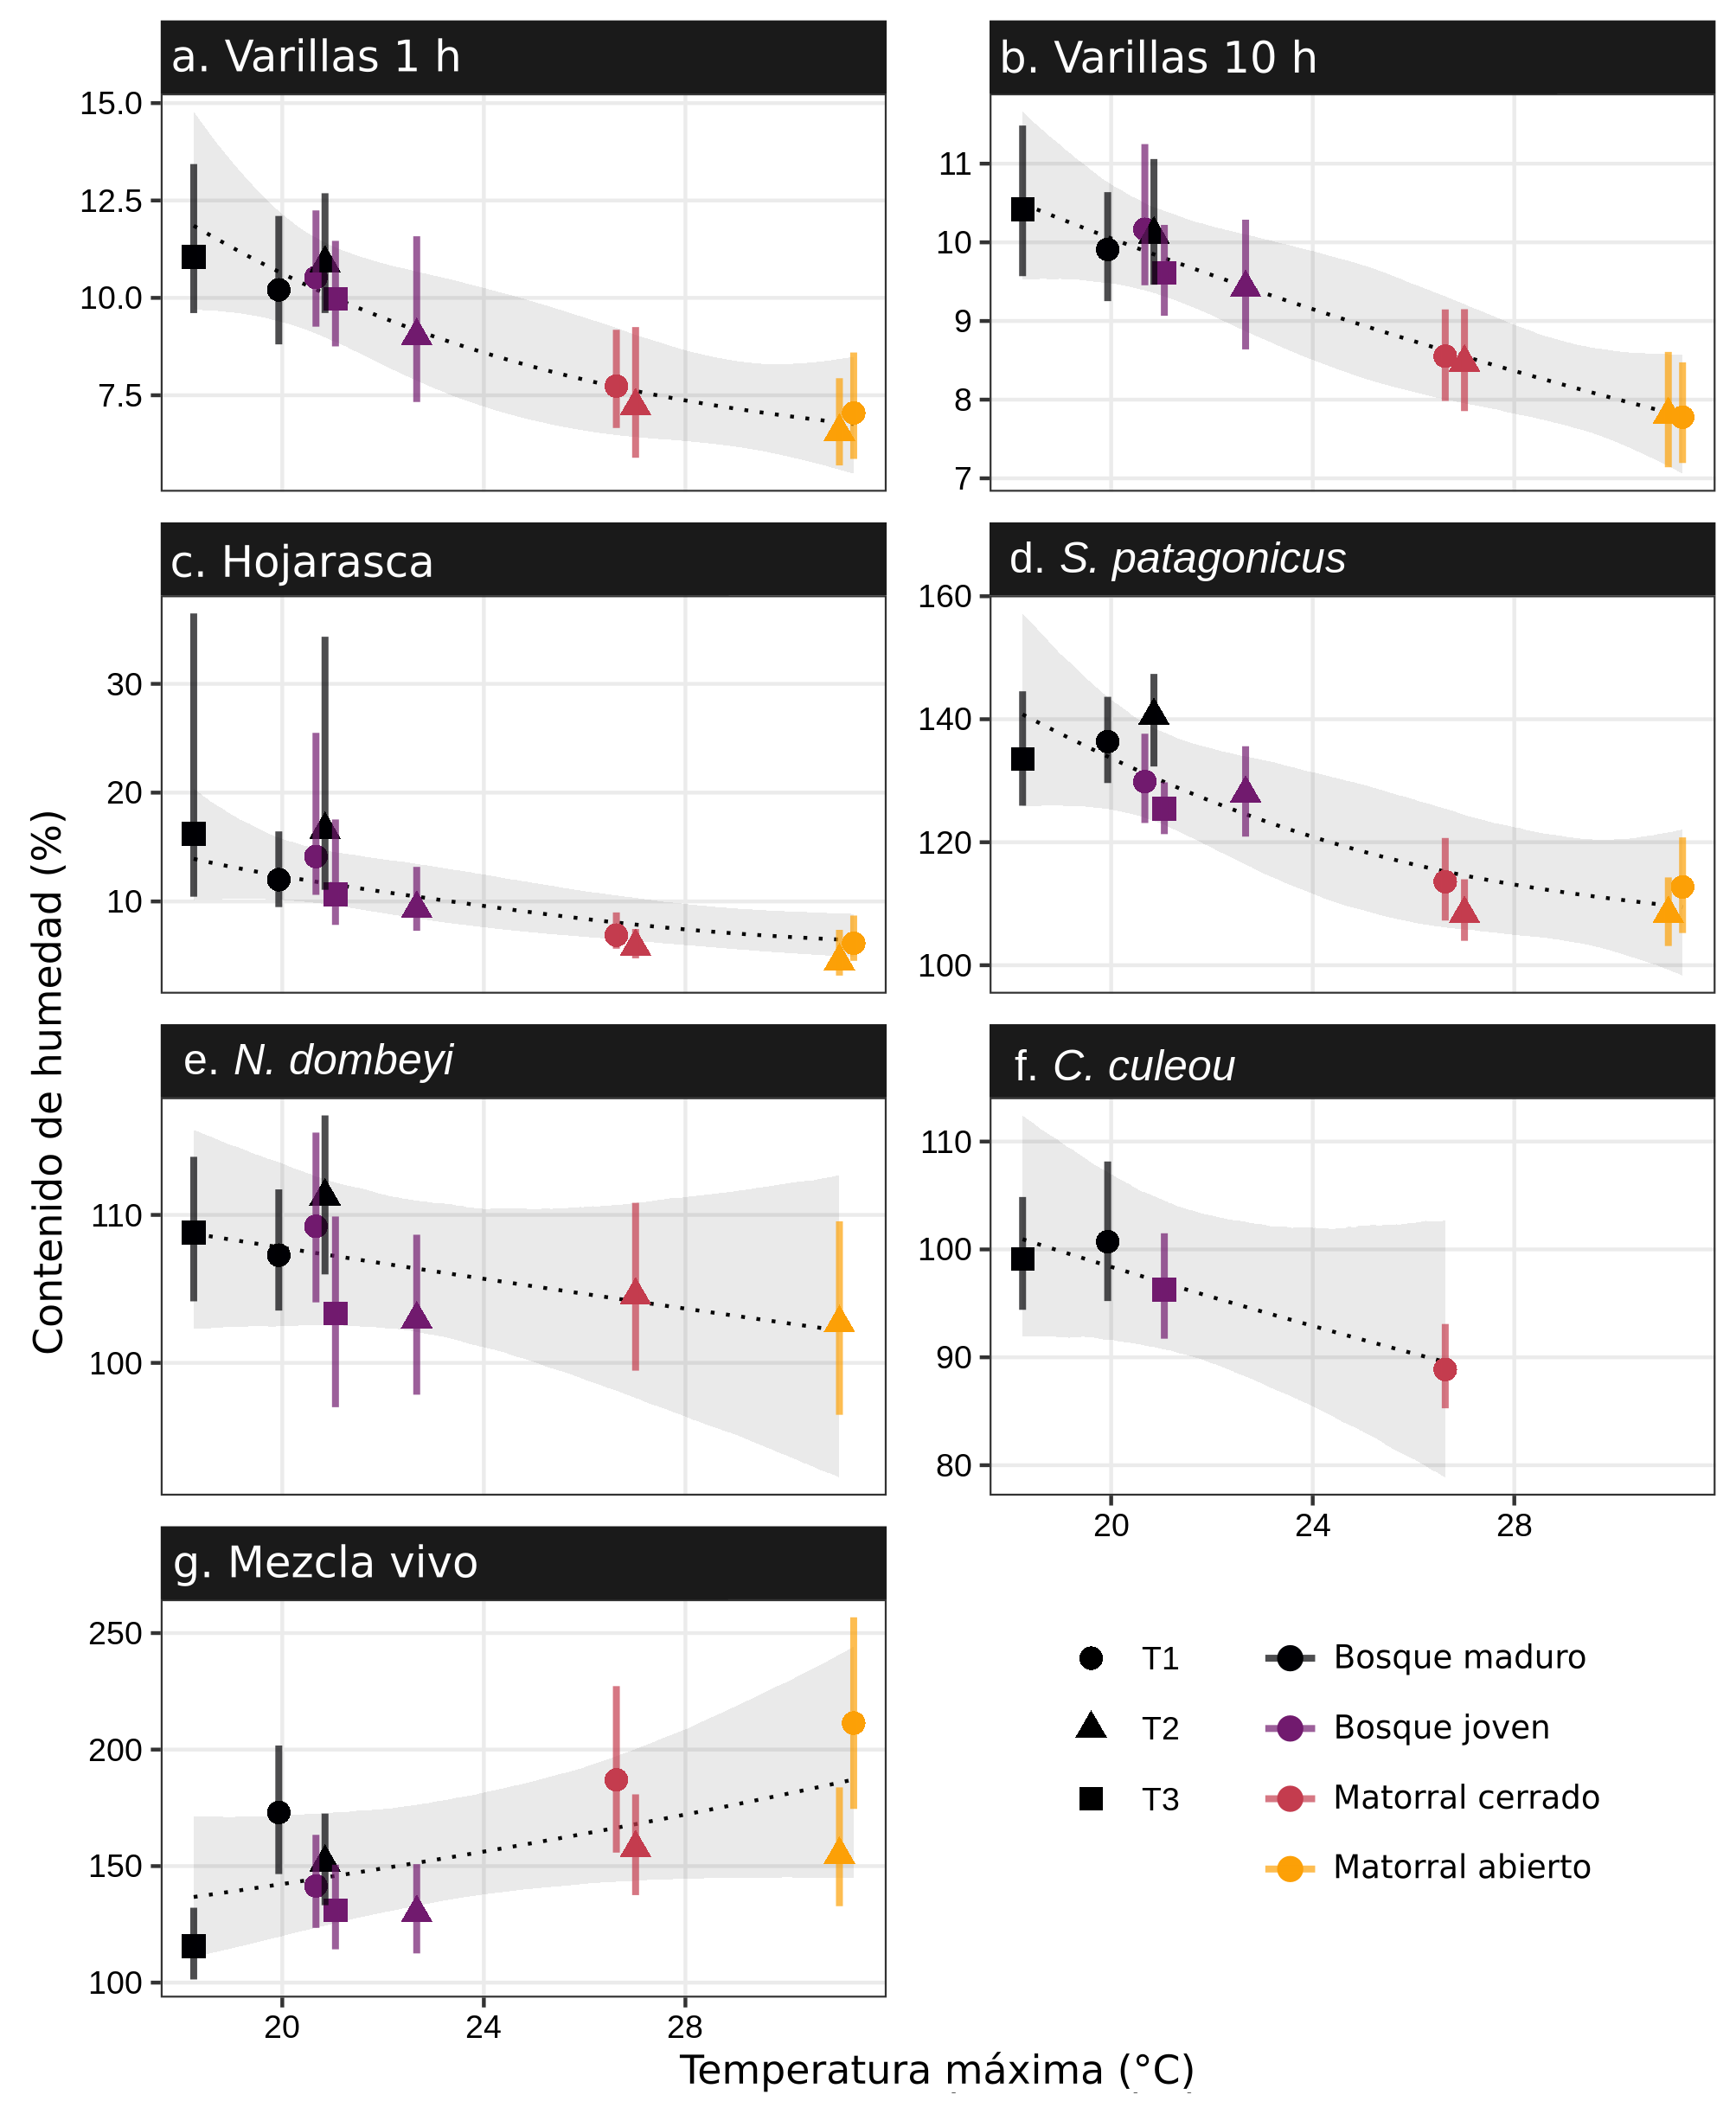
\includegraphics[width=16cm]{figuras/cap2/S09) fmc_temperature.png}
    \caption[Humedad del combustible en función de la temperatura del aire.]{Contenido de humedad promedio estimado en función de la temperatura máxima diaria promediada durante el período de estudio por sitio. Los puntos representan la media posterior para cada sitio, y las barras, los intervalos de confianza del 95 \% (mismos valores que en la figura~\ref{fig:cap2-03}, panel derecho). El efecto ajustado de la temperatura se muestra con la línea discontinua (media posterior) y la banda gris (IC del 95\%). Los modelos tuvieron la misma estructura y las mismas previas que los ajustados utilizando el DPV máximo, descritos en la Sección~\ref{cap2:humedad-methods} y en el Apéndice~\ref{append:moisture-models}.}
    \label{fig:cap2-S09}
\end{figure}

\begin{figure}
    \centering
    \caption[Humedad del combustible en función del tiempo.]{Contenido de humedad del combustible a lo largo de la estación seca por comunidad, transecta y tipo de combustible. La línea muestra el contenido de humedad promedio estimado por los GLMMs (medias posteriores), y la banda más oscura representa el intervalo de confianza del 95 \% para estas medias. Los puntos muestran los datos observados, y la banda más amplia y clara muestra el intervalo de mayor densidad del 95 \% para los datos (donde aproximadamente debería encontrarse el 95 \% de los puntos). Tratamos las fechas como un efecto aleatorio (variable categórica), pero las predicciones están conectadas con líneas para mejorar la visibilidad. (Ver figuras en las siguientes páginas).}
    \label{fig:cap2-S10-legend}
\end{figure}

\addtocounter{figure}{-1}

\begin{figure}
    \centering
    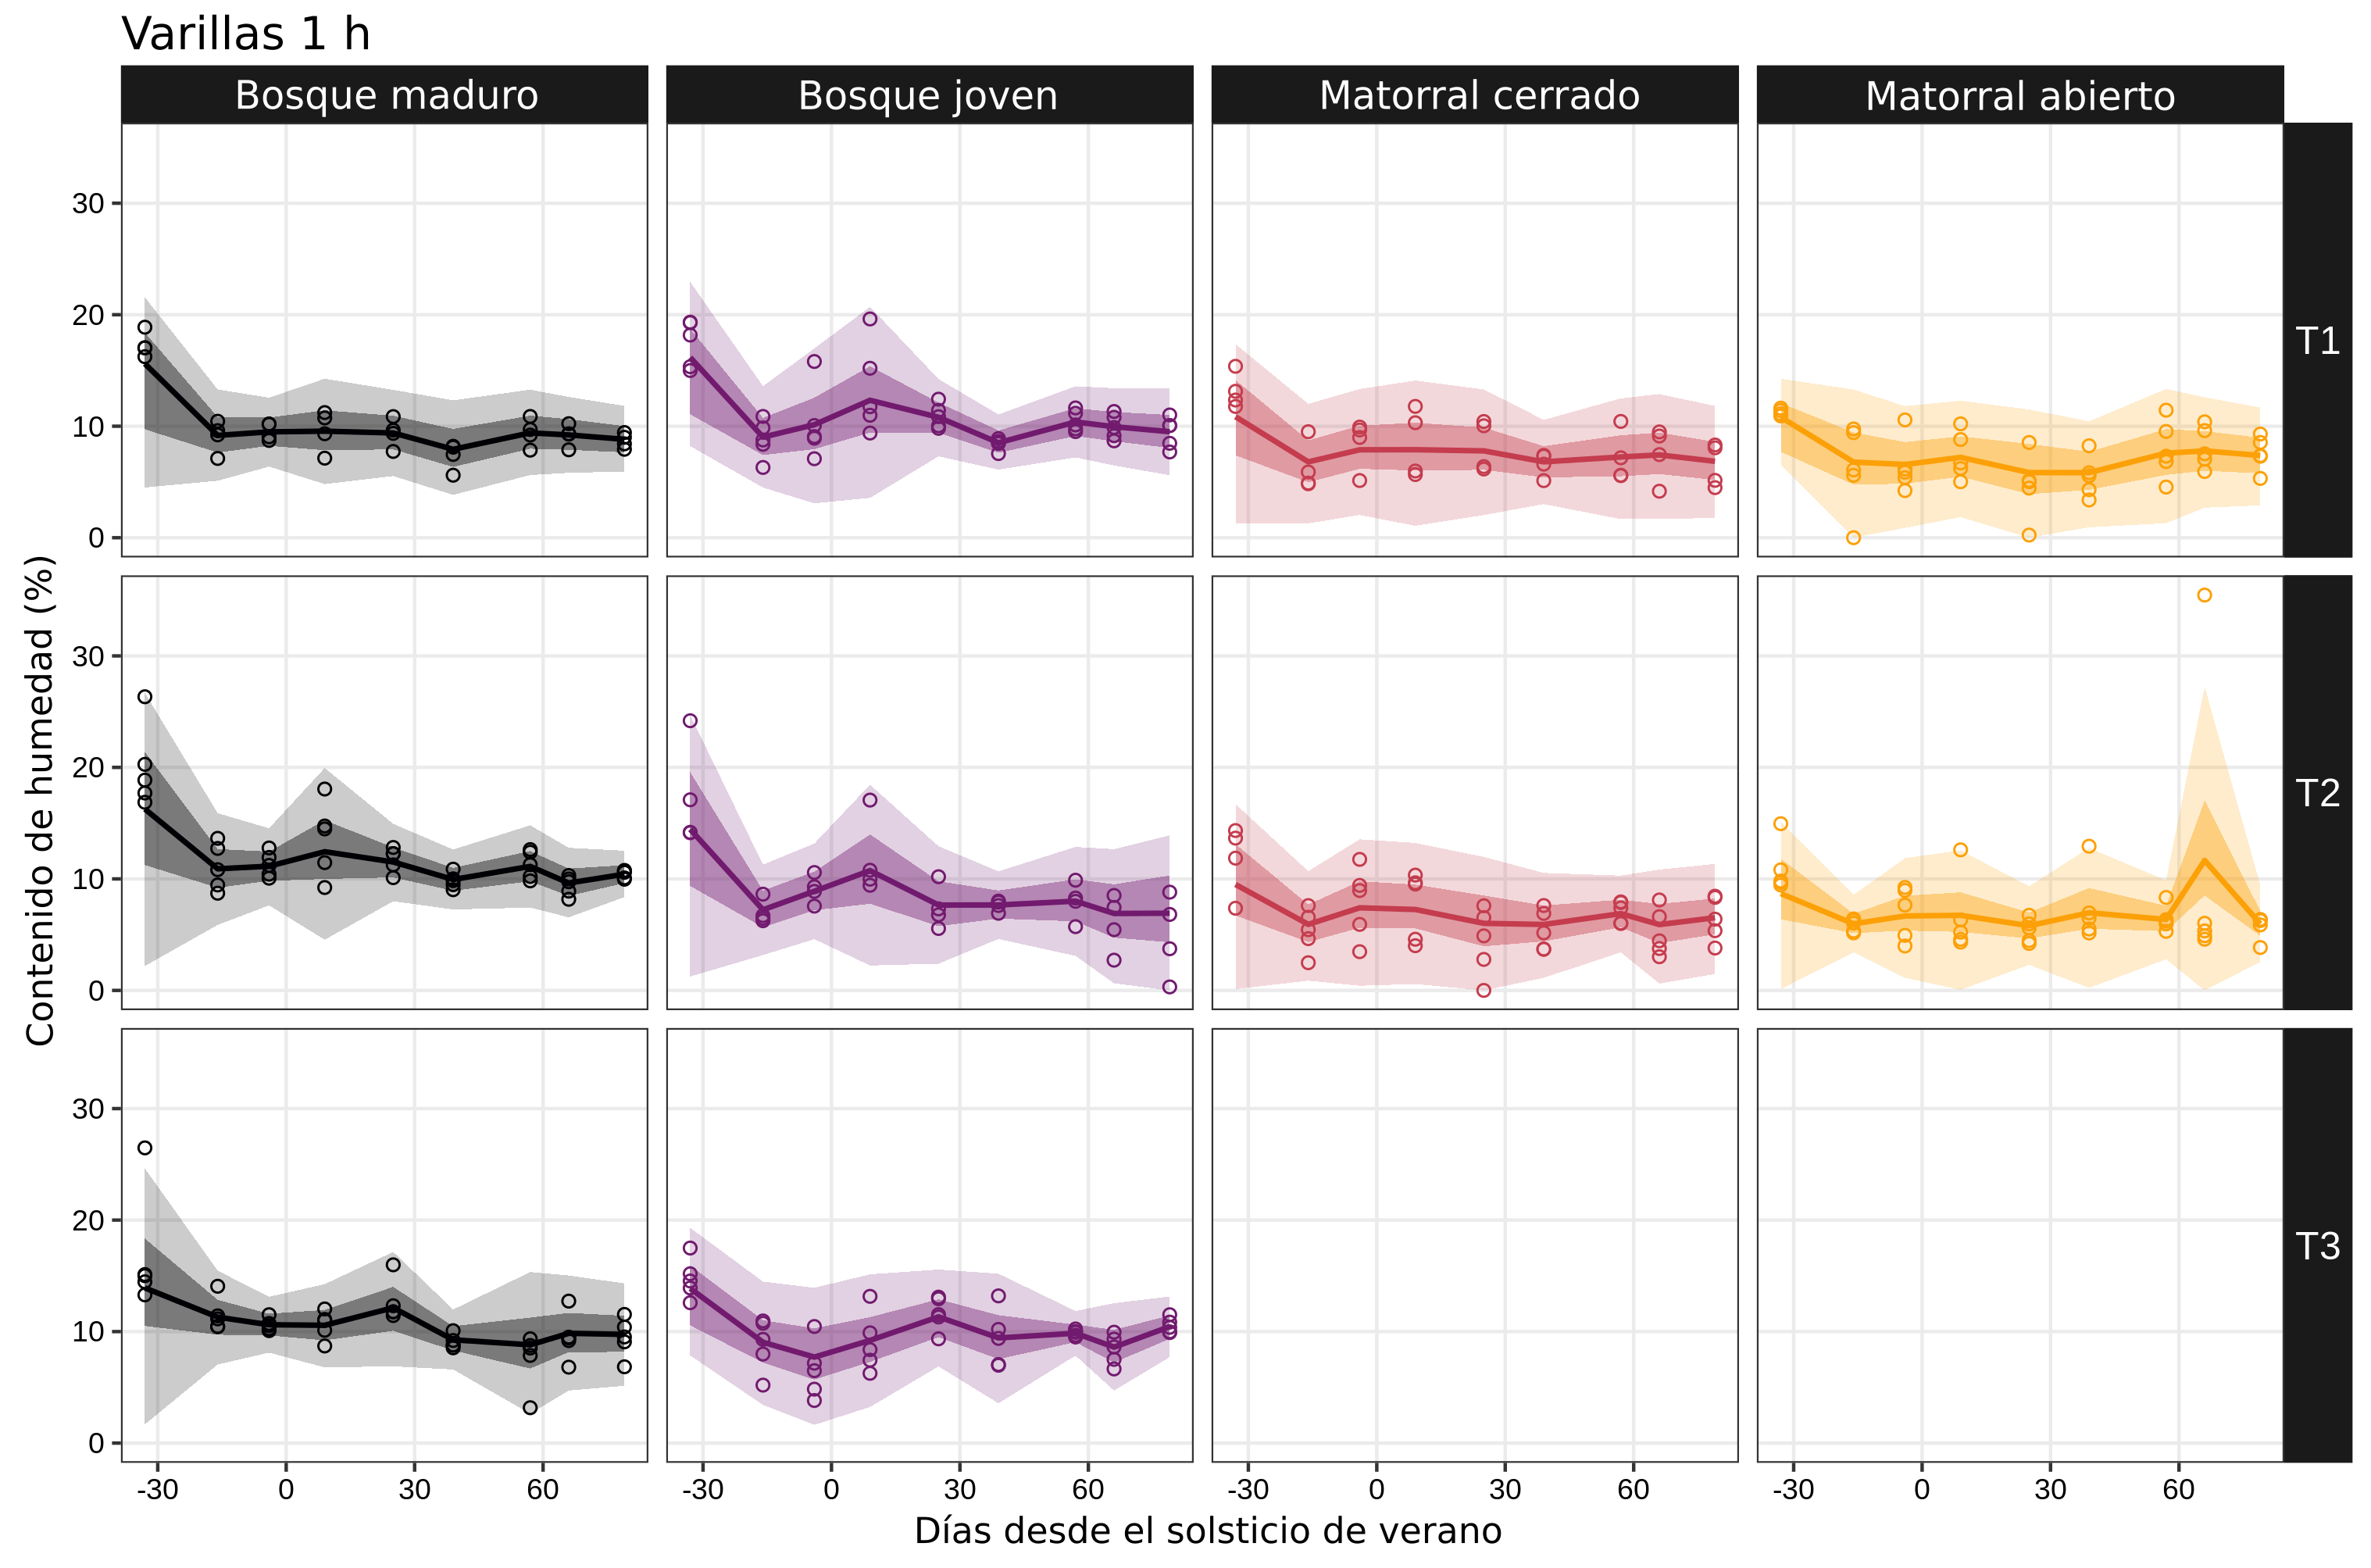
\includegraphics[width=16cm]{figuras/cap2/S10) 1h.png}
    \captionsetup{list=no}
    \caption{Ver leyenda arriba.}
    \label{fig:cap2-S10}
\end{figure}

\begin{figure}
    \centering
    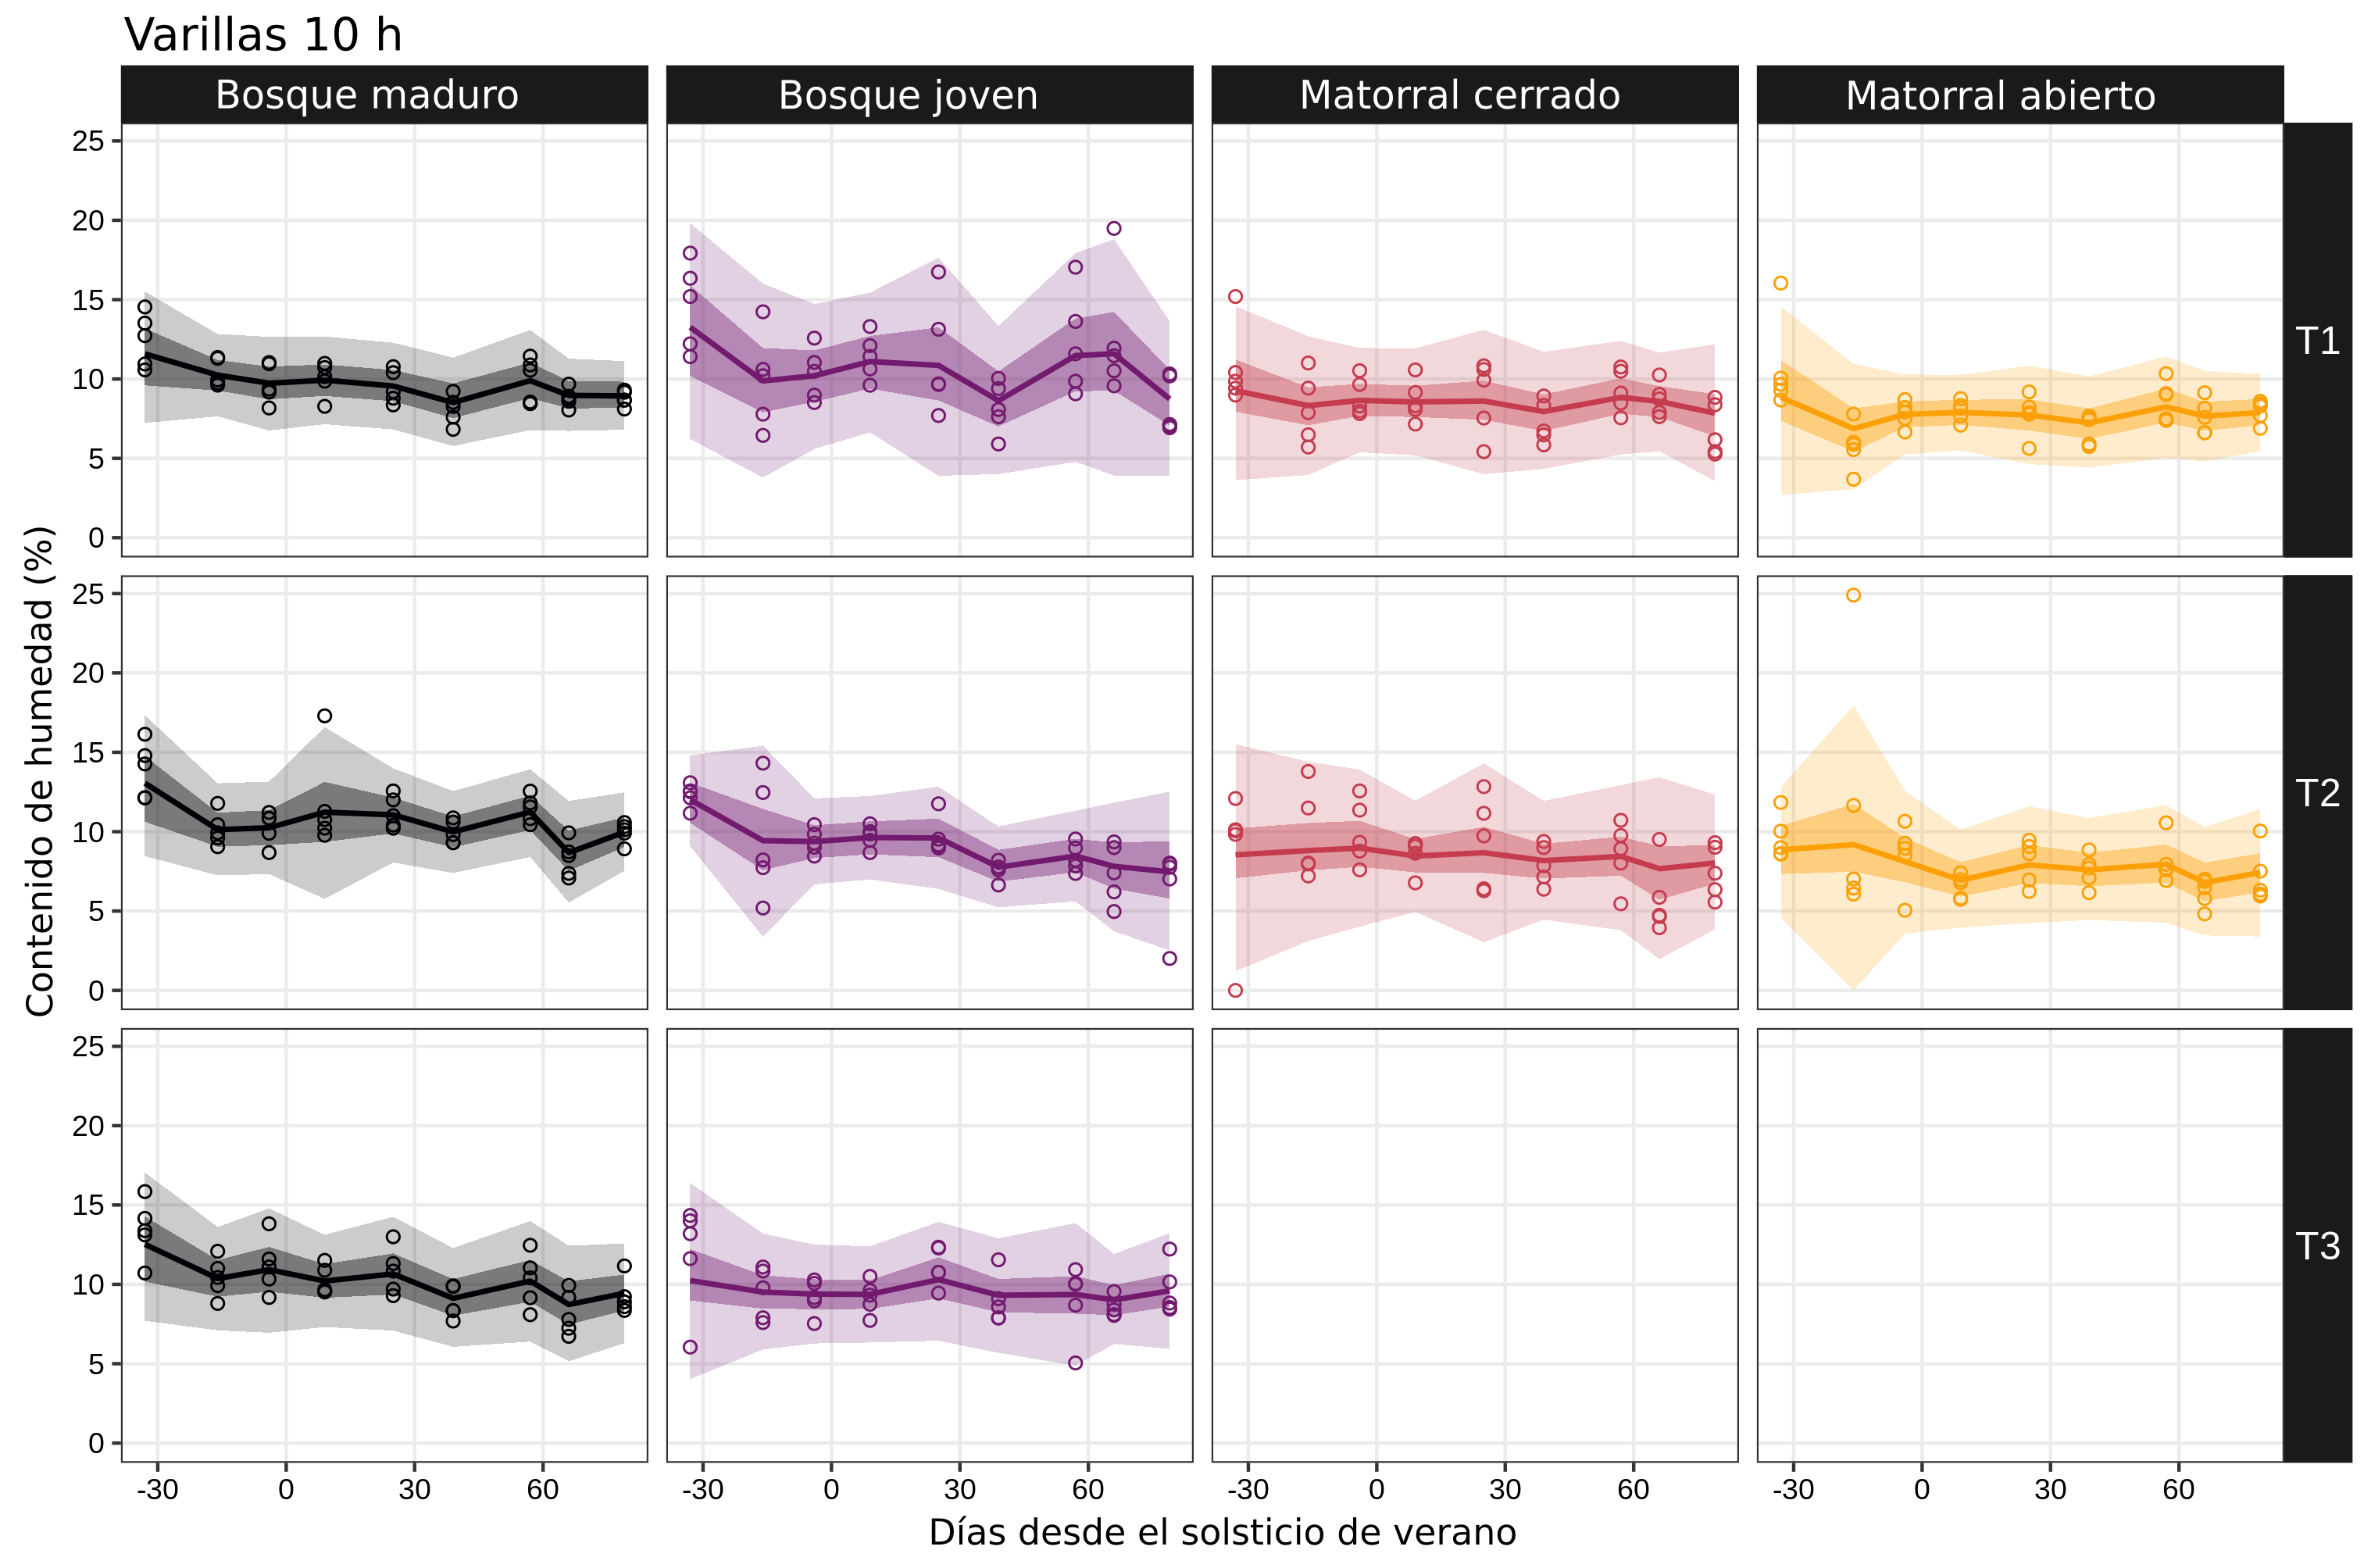
\includegraphics[width=16cm]{figuras/cap2/S11) 10 h.png}
    \captionsetup{list=no}
    \caption{Ver~\ref{fig:cap2-S10-legend}}
    \label{fig:cap2-S11}
\end{figure}

\begin{figure}
    \centering
    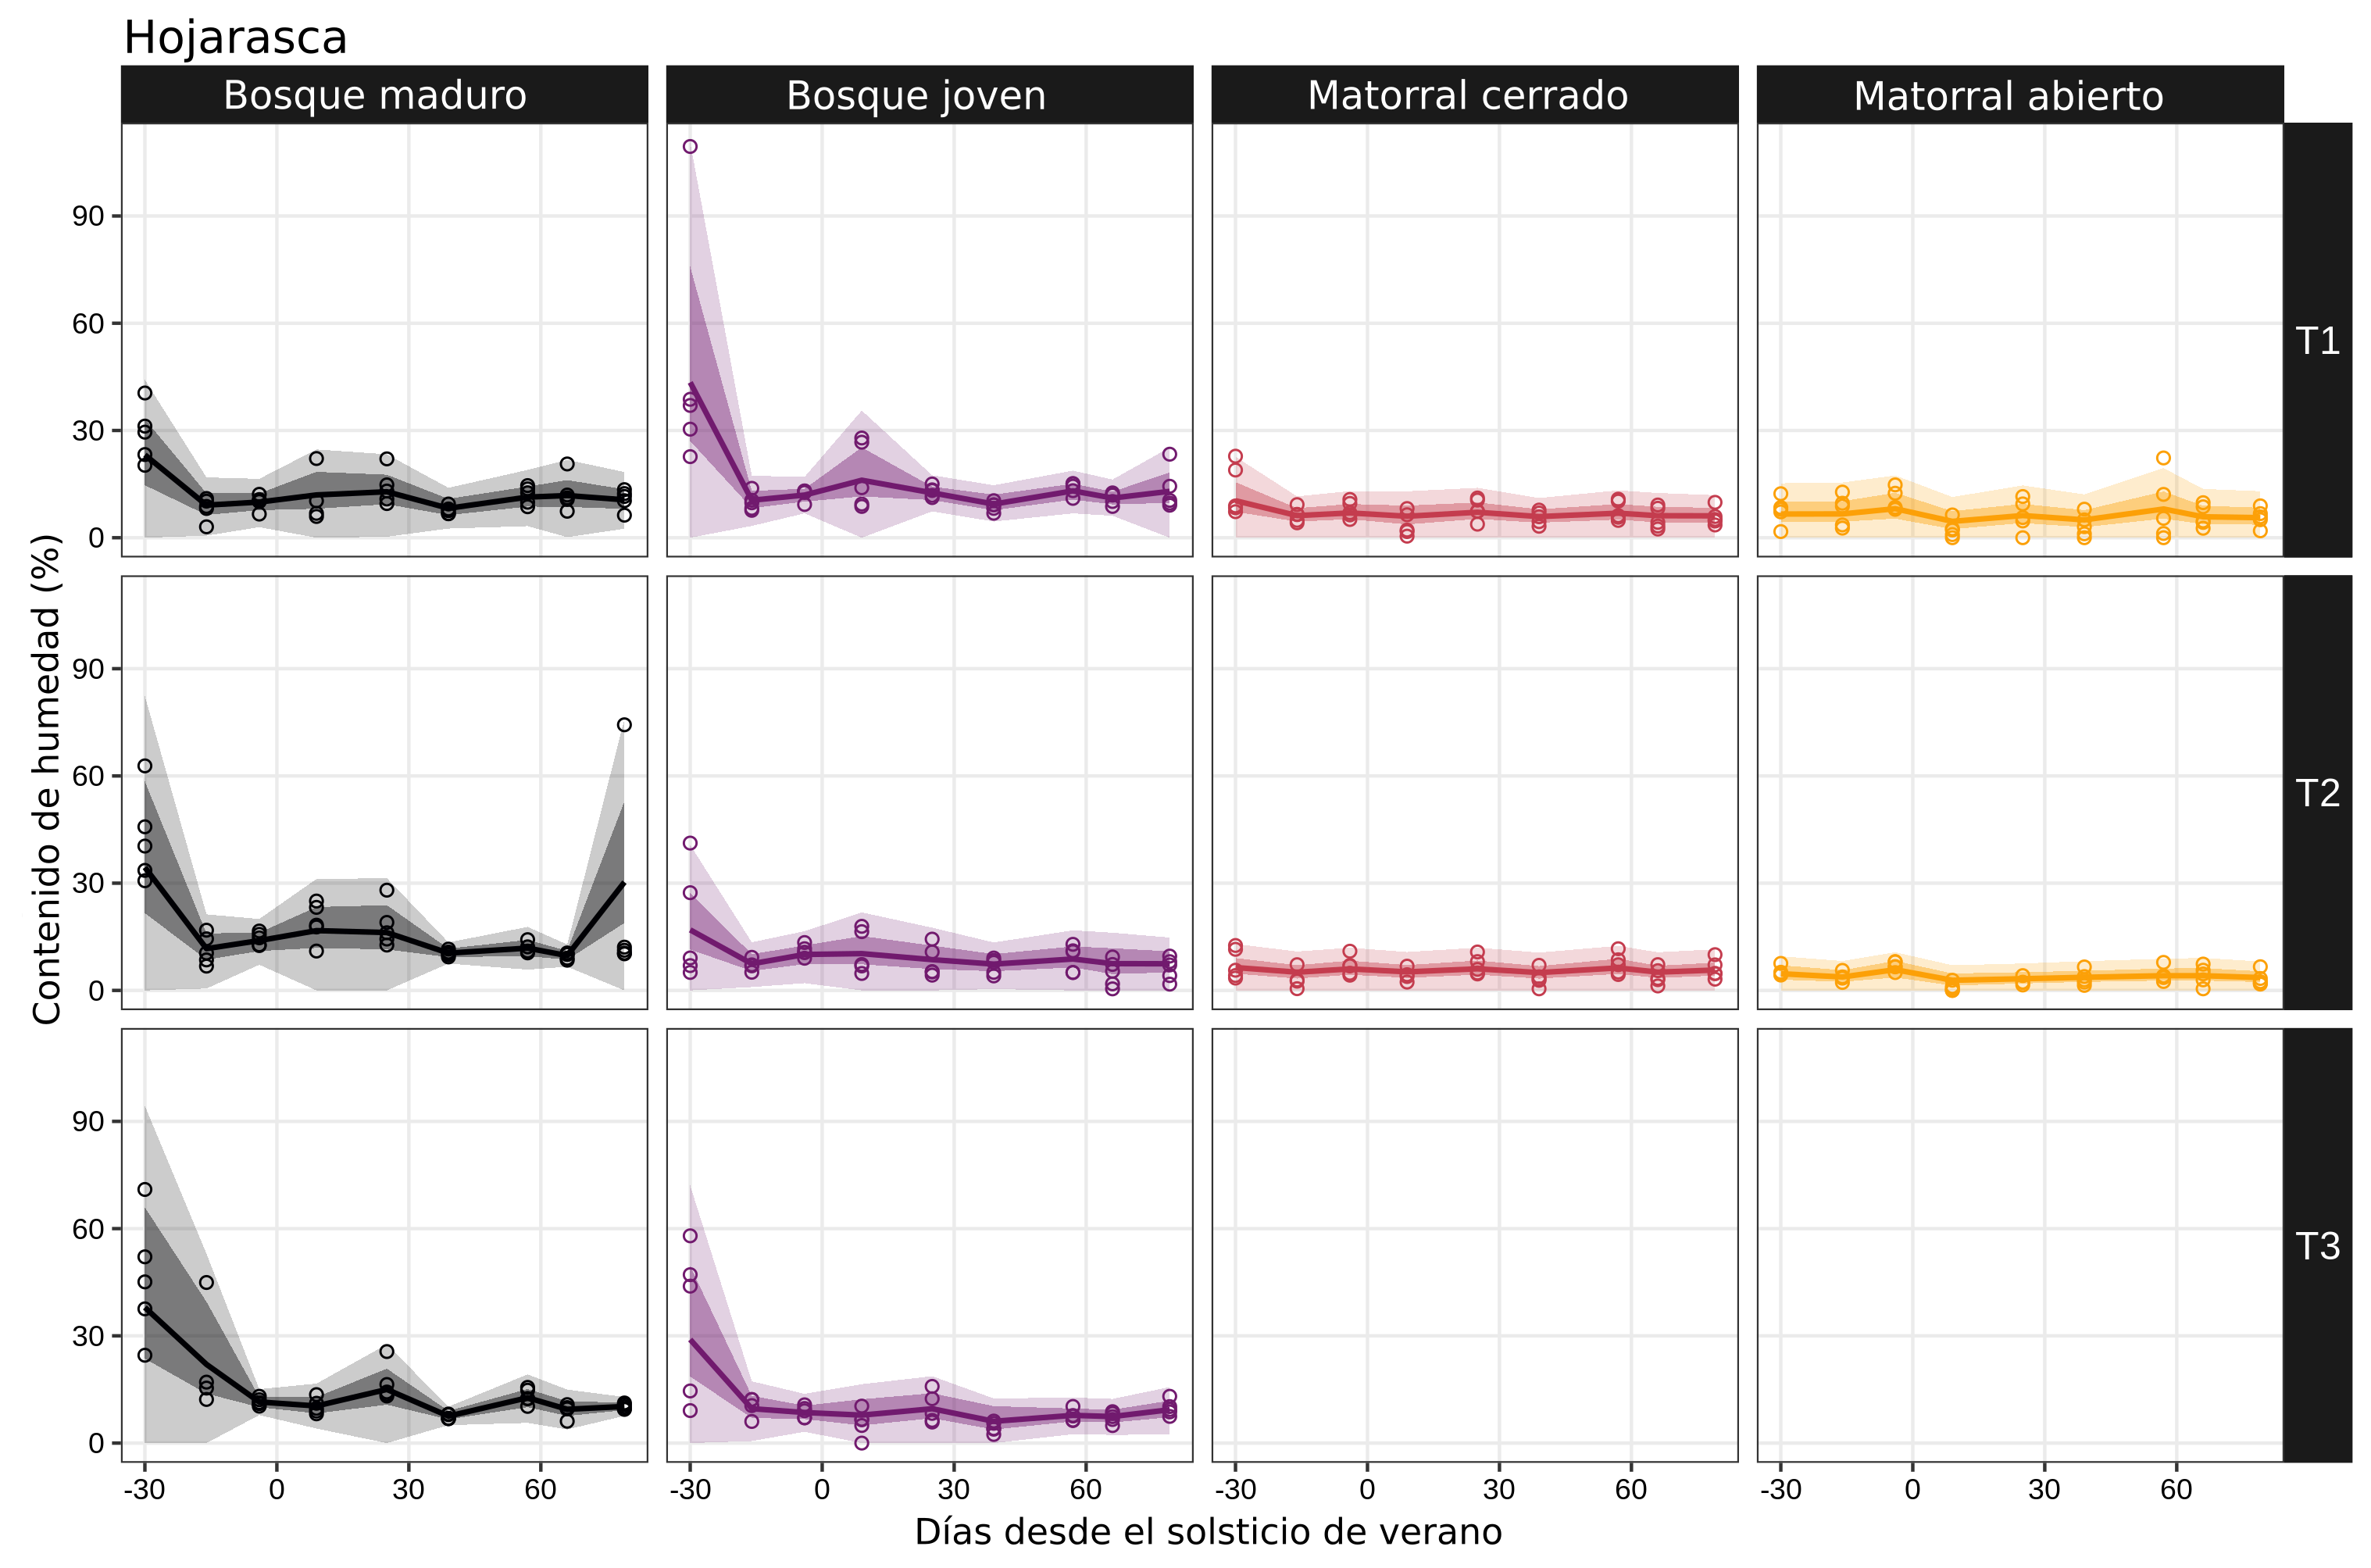
\includegraphics[width=16cm]{figuras/cap2/S12) litter.png}
    \captionsetup{list=no}
    \caption{Ver~\ref{fig:cap2-S10-legend}}
    \label{fig:cap2-S12}
\end{figure}

\begin{figure}
    \centering
    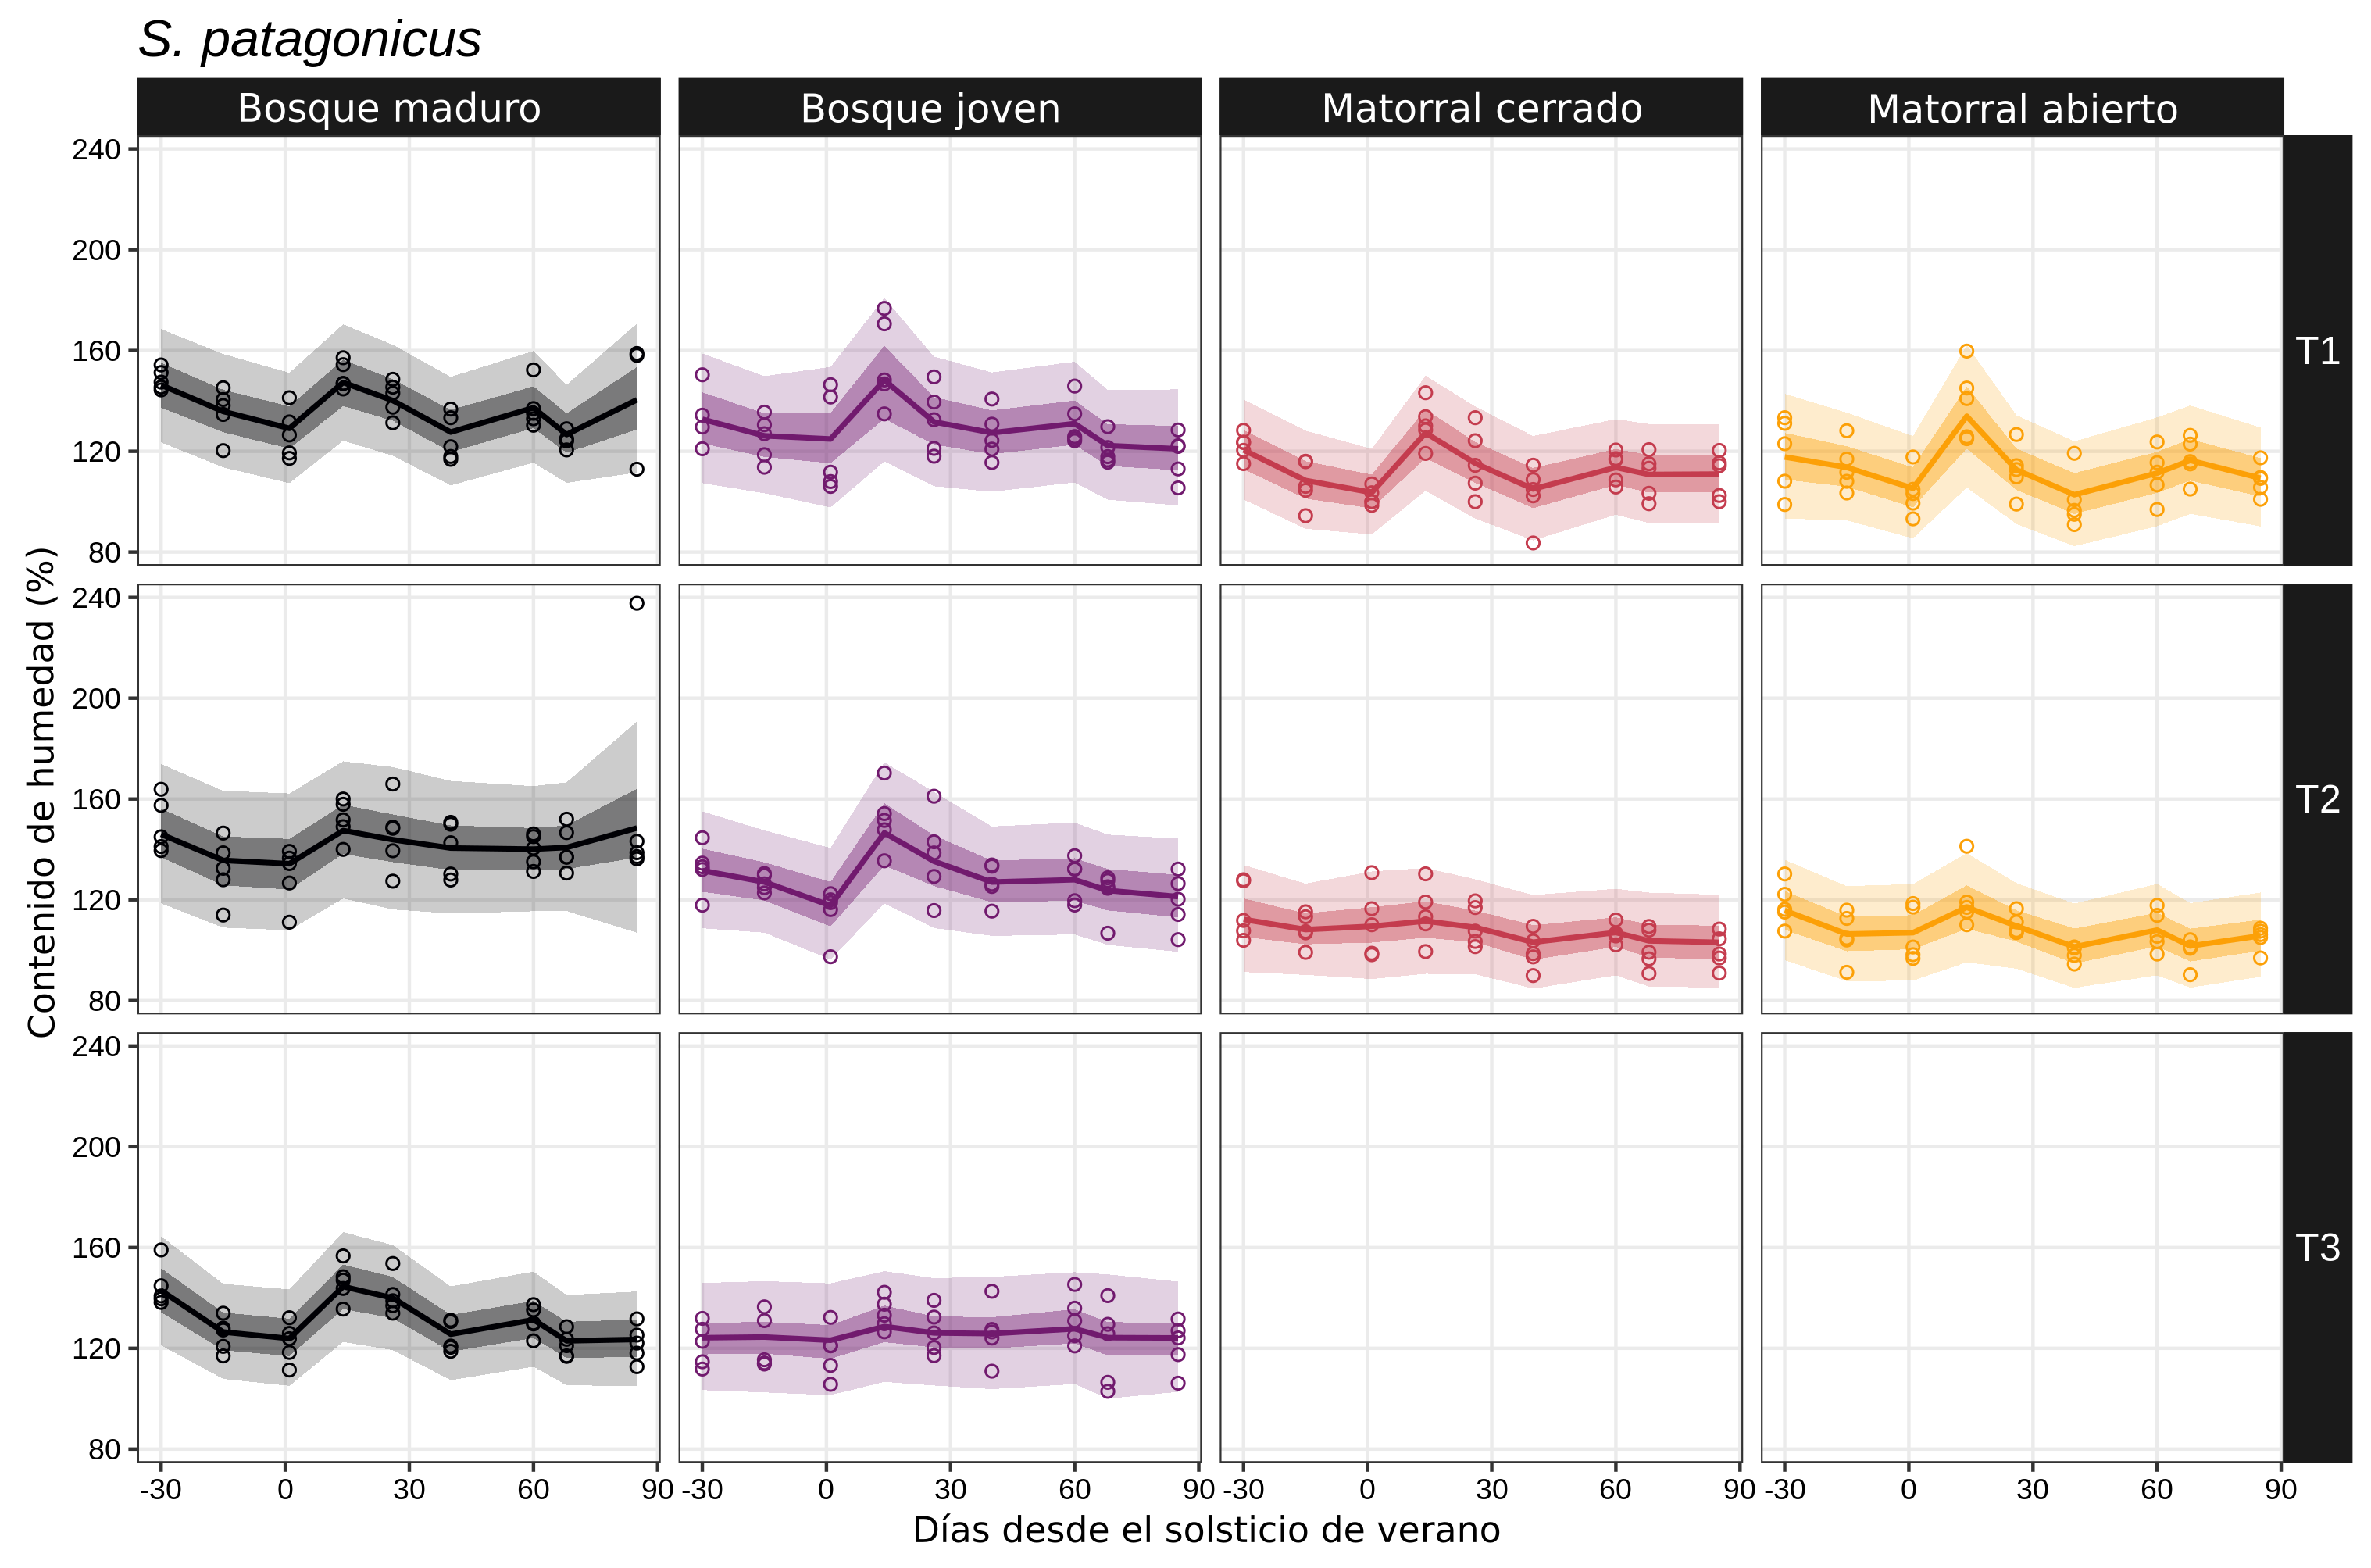
\includegraphics[width=16cm]{figuras/cap2/S13) laura.png}
    \captionsetup{list=no}
    \caption{Ver~\ref{fig:cap2-S10-legend}}
    \label{fig:cap2-S13}
\end{figure}

\begin{figure}
    \centering
    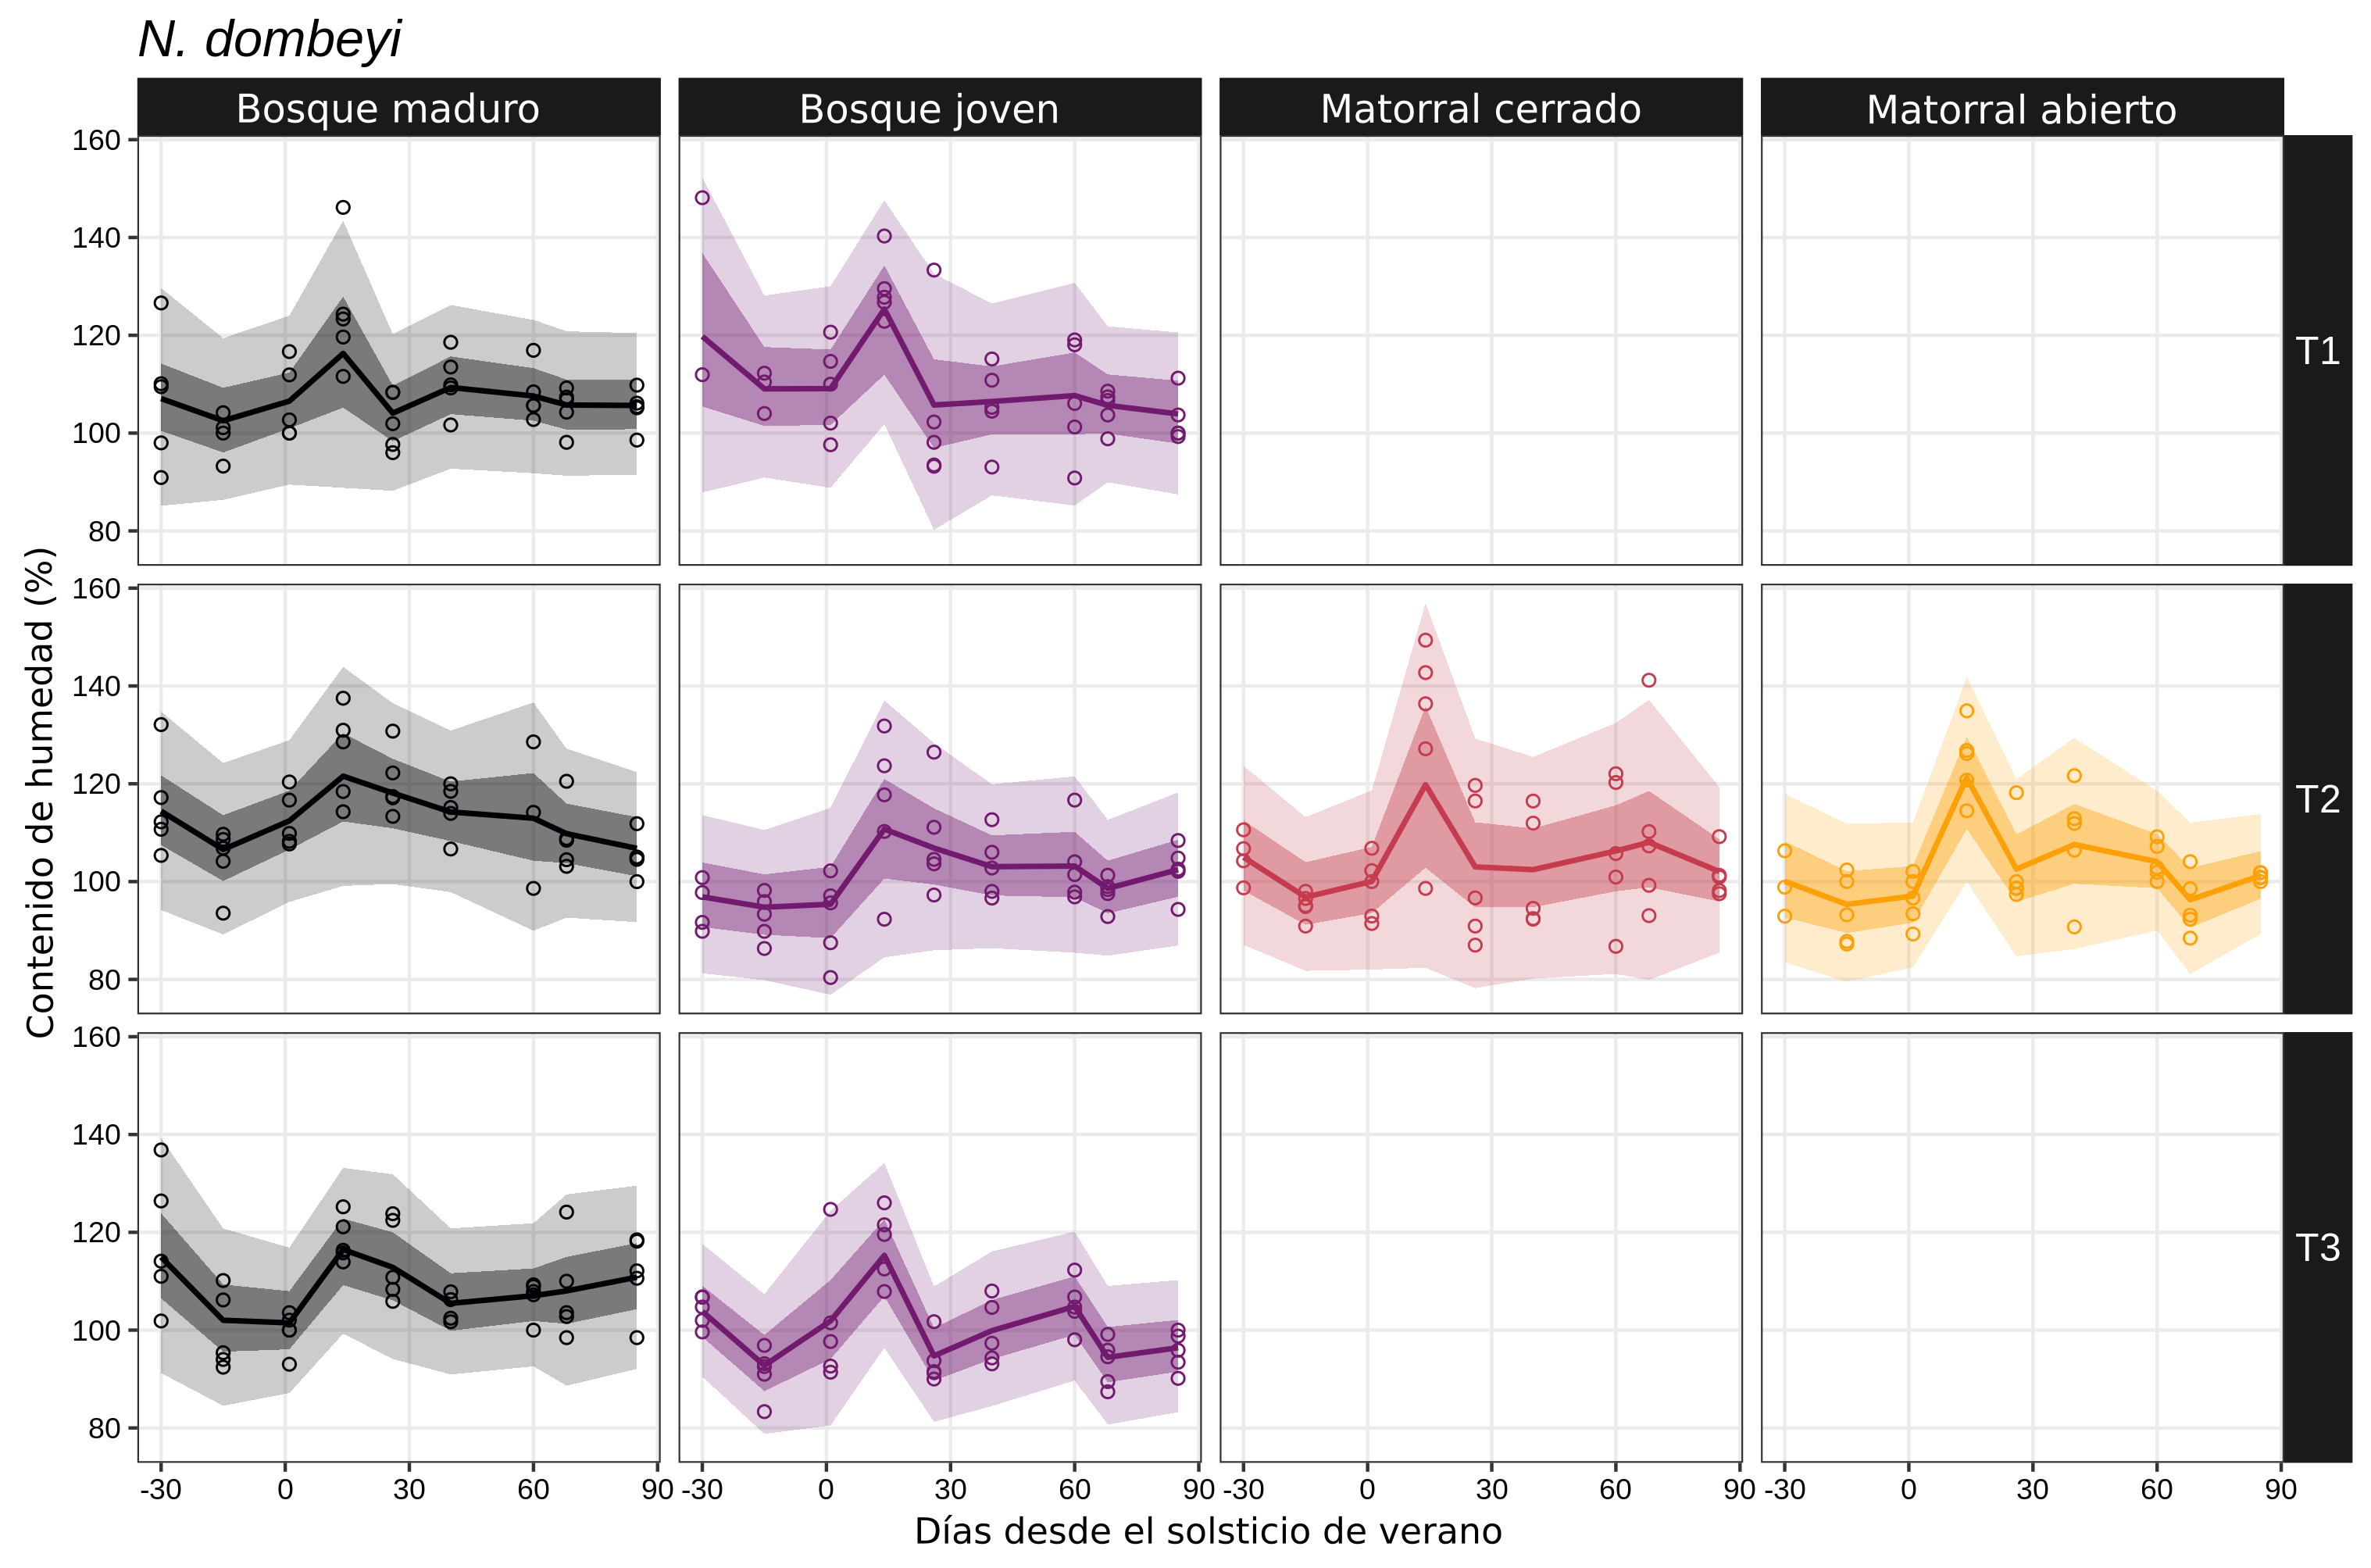
\includegraphics[width=16cm]{figuras/cap2/S14) coihue.png}
    \captionsetup{list=no}
    \caption{Ver~\ref{fig:cap2-S10-legend}}
    \label{fig:cap2-S14}
\end{figure}

\begin{figure}
    \centering
    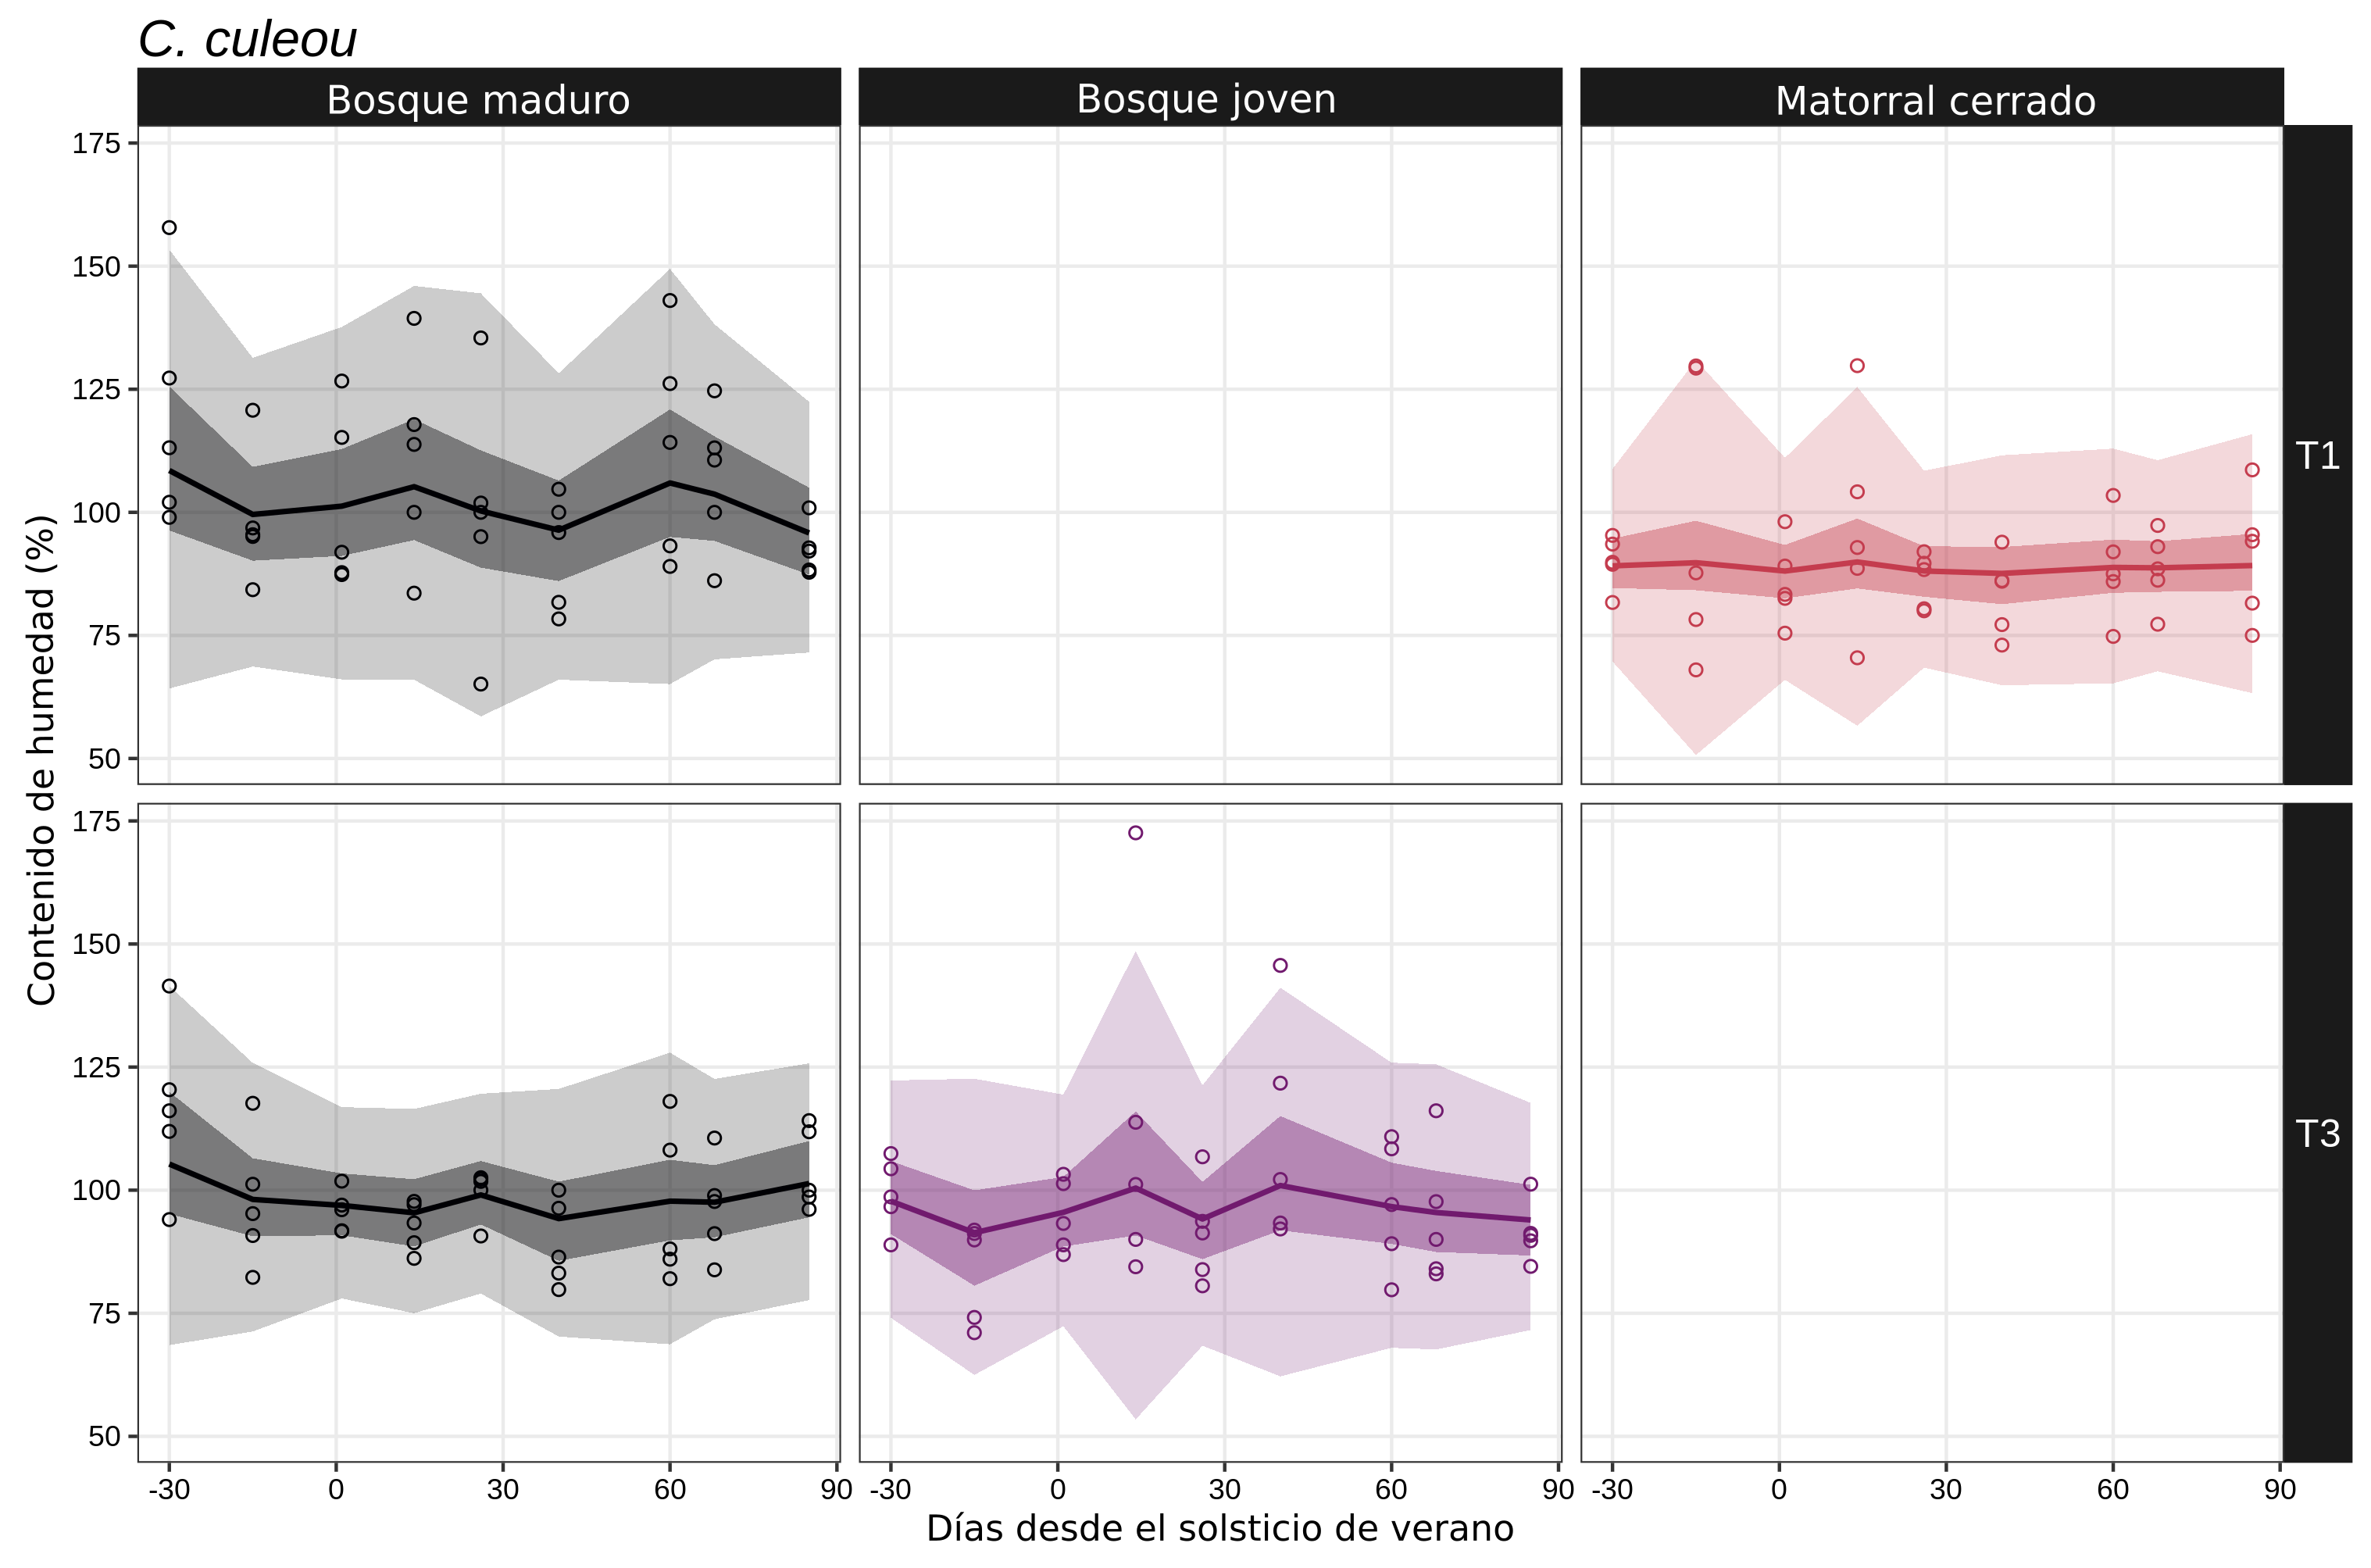
\includegraphics[width=16cm]{figuras/cap2/S15) cania.png}
    \captionsetup{list=no}
    \caption{Ver~\ref{fig:cap2-S10-legend}}
    \label{fig:cap2-S15}
\end{figure}


\begin{figure}
    \centering
    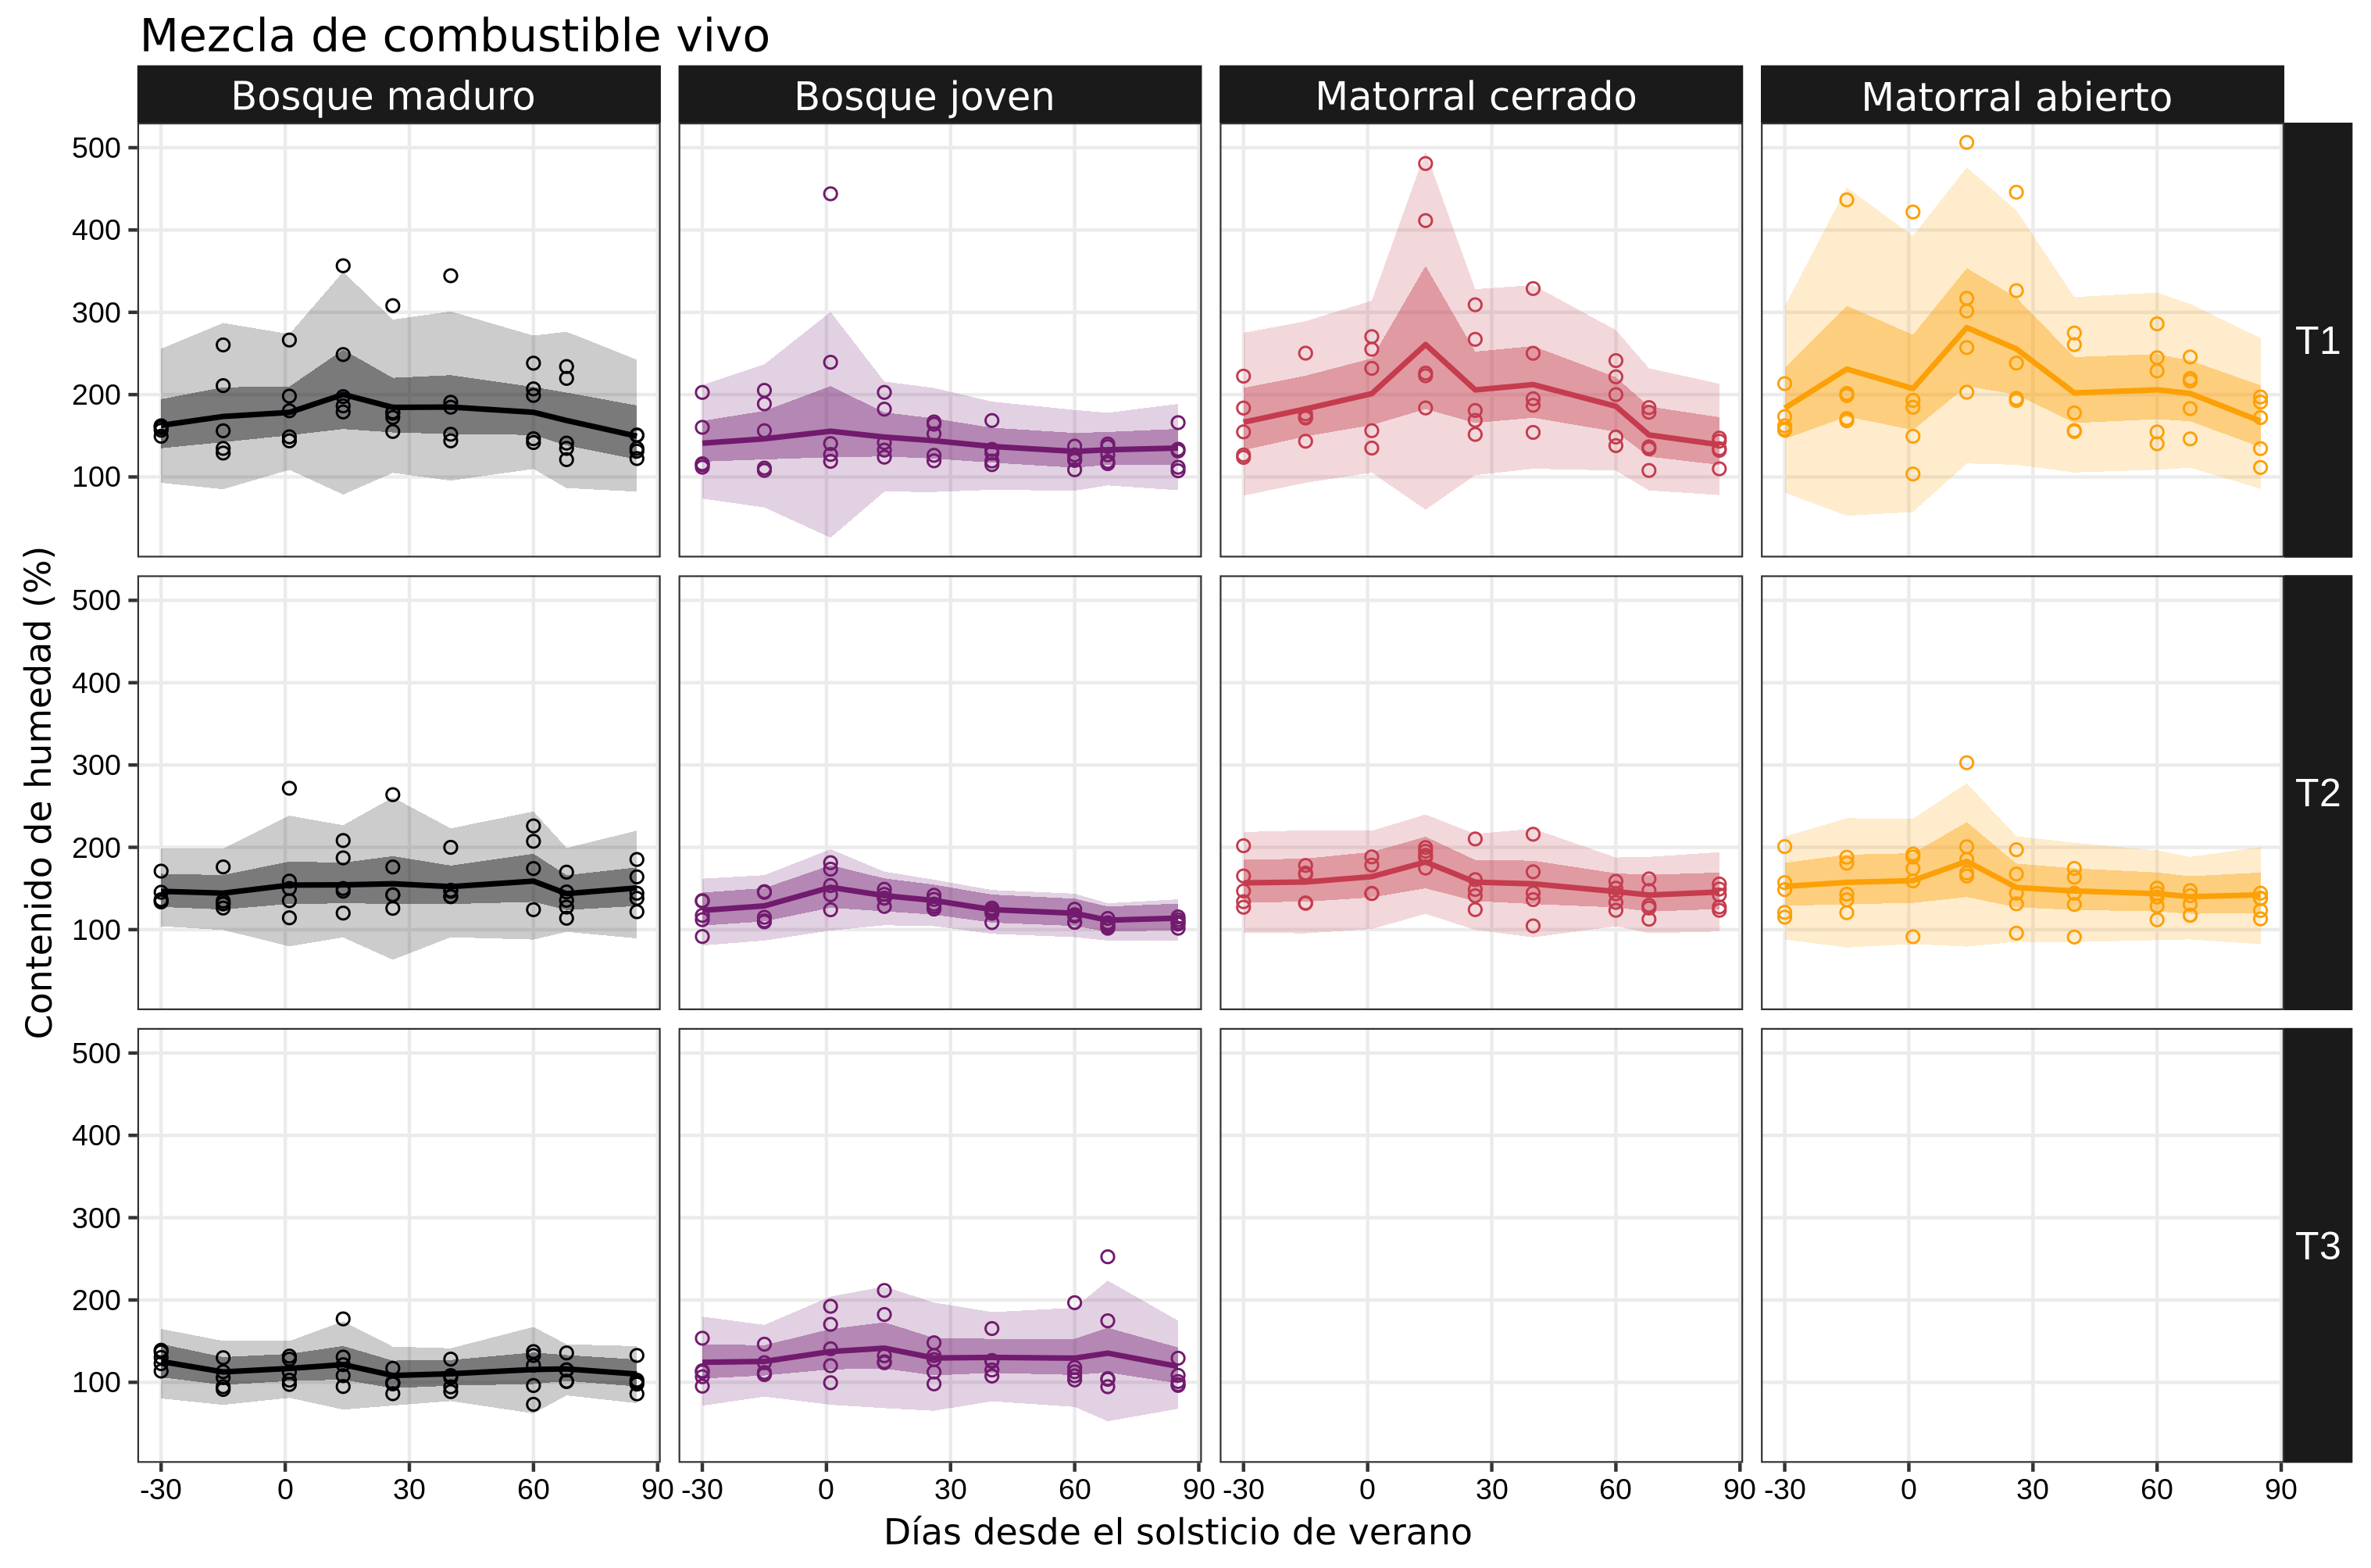
\includegraphics[width=16cm]{figuras/cap2/S16) vivos.png}
    \captionsetup{list=no}
    \caption{Ver~\ref{fig:cap2-S10-legend}}
    \label{fig:cap2-S16}
\end{figure}

\FloatBarrier

\section{Especificación completa de modelos}


\subsection{Modelo de déficit de presión de vapor}\label{append:microclimate-models}

Para comparar el DPV (Déficit de Presión de Vapor) entre comunidades dentro de cada transecta, ajustamos un modelo jerárquico asumiendo una distribución Log-Normal para las series temporales diarias de DPV y considerando la correlación temporal entre observaciones mediante una función de correlación autorregresiva de orden 1 (\texttt{corAR1}). Incluimos efectos fijos de la comunidad sobre la media ($\mu$) y el desvío estándar ($\sigma$) en la escala logarítmica, y un efecto aleatorio del sitio sobre $\mu$. 

\begin{equation}
    \begin{aligned}
    \text{log}(\textbf{y}_{cs}) &\sim \text{NMV}(\boldsymbol{\mu}_{cs}, \boldsymbol{\Sigma}_{c}) \\
    \Sigma_{c,ij} &= \sigma_{c}^{2} \ \rho^{\text{k}_{ij}} \\
    \\
    \mu_{cs} &= \eta_{c} + \delta_{s} \\
    \eta_{c} &\sim \text{Normal}(0, 5) \\
    \delta_{s} &\sim \text{Normal}(0, \tau) \\
    \tau &\sim \text{Normal}(0, 1)\text{T}[0, ] \\
    \\
    \sigma_{c} &\sim \text{Normal}(0, 1.5)\text{T}[0, ] \\
    \rho &\sim \ \text{Uniforme}(0, 1). \\
    \end{aligned}
\end{equation}
  
\noindent $\textbf{y}_{cs}$ es el vector de longitud $N = 119$ con los valores diarios máximos de DPV (entre el 18/11/2019 y el 15/03/2020) para la comunidad $c \in \{1, ..., 4\}$ y el sitio $s \in \{1, ..., 10\}$. $\text{k}_{ij}$ es la distancia temporal (en días) entre las observaciones $i$ y $j$, donde $i$ y $j \in \{1, ..., N\}$.  
$\boldsymbol{\mu}_{cs}$ es un vector que repite $\mu_{cs}$ $N$ veces, lo cual representa la mediana del DPV en la comunidad $c$ y el sitio $s$ en la escala logarítmica.  
$\sigma_{cs}$ es la desviación estándar de $\text{log}(\textbf{y}_{cs})$,  
$\rho_{cs}$ es el coeficiente de correlación temporal entre observaciones consecutivas en la escala logarítmica,  
y NMV denota una distribución Normal Multivariada.  
$\eta$ son los efectos fijos para $\mu$, que varían entre comunidades, mientras que $\delta$ son efectos aleatorios a nivel de sitio. 
  
La distribución Normal está parametrizada con media y desvío estándar. T[,] indica distribuciones truncadas en los valores indicados por el intervalo, donde un valor faltante indica $\pm \ \infty$. Como la respuesta asume Log-Normal, su media se calcula como:

\[
\text{E}(\textbf{y}_{cs}) = \text{exp}\left(\mu_{cs} + \frac{\sigma_{cs}^2}{2}\right),
\]

mientras que:

\[
\text{exp}(\mu_{cs}) = \text{mediana}(\textbf{y}_{cs}).
\]

Corrimos 10 cadenas markovianas durante 2000 iteraciones, dejando 1000 para la fase de calentamiento. Considerando todos los parámetros y cantidades derivadas calculadas en Stan (e.g., medias), el valor máximo de $\hat{\text{R}}$ fue 1.003, lo que indica convergencia, y el tamaño efectivo de muestra más pequeño fue 2408.  

\subsection{Modelos de humedad del combustible}\label{append:moisture-models}

Dado que nos interesaba la variación en el contenido de humedad entre comunidades mediada por el microclima, ajustamos un Modelo Lineal Generalizado Mixto (GLMM, por sus siglas en inglés) para cada tipo de combustible, especificando una regresión del contenido de humedad en función del DPV (Déficit de Presión de Vapor) a nivel de sitio, utilizando como predictora el promedio diario máximo de DPV de cada sitio. Modelamos la media de la respuesta con un enlace log, incluyendo efectos aleatorios de sitio (combinaciones de comunidad y transecta), fecha y su combinación. Inicialmente intentamos ajustar una estructura de correlación temporal para los efectos aleatorios de la fecha, pero con solo nueve fechas no pudimos estimar el parámetro de correlación, por lo que asumimos efectos independientes. No incluimos el factor comunidad en los modelos porque suponíamos que el mayor efecto de la comunidad sobre el contenido de humedad estaría mediado por el microclima y porque la comunidad y el DPV están altamente correlacionados, lo que habría dificultado la estimación del efecto del DPV y la interpretación de los resultados.  

Para los combustibles vivos asumimos una distribución Gamma, ya que su asimetría permitió un buen ajuste a los datos. En el caso de los combustibles muertos, se observaron valores extremos del contenido de humedad cercanos a cero, lo que llevaba a la distribución Gamma a estimar una varianza alta para acomodar estos valores bajos, implicando también una alta densidad en valores de contenido de humedad elevados que no eran compatibles con los datos. Esto nos llevó a preferir distribuciones Normales truncadas en 0 para el contenido de humedad de los combustibles muertos, lo que permite una mayor densidad en valores cercanos a cero sin ajustar una varianza extrema.  

A continuación especificamos completamente el modelo para la mezcla de combustibles vivos, que fue el más complejo, y mencionamos las diferencias para otros tipos de combustible más abajo.  

\[
\begin{aligned}
    \text{y}_{dsp} &\sim \text{Gamma}(\alpha_{ds}, \beta_{dsp})\\
    \alpha_{ds} &= \frac{1}{\phi_{ds}}\\
    \beta_{dsp} &= \frac{1}{\mu_{dsp} \ \phi_{ds}}.\\
\end{aligned}
\]

\noindent Aquí, $\text{y}_{dsp}$ es el contenido de humedad en la fecha $d \in \{1, ..., 9\}$, sitio $s \in \{1, ..., 10\}$ y parcela de muestreo $p \in \{1, ..., 50\}$ (había 5 parcelas de muestreo por sitio). $\alpha$ y $\beta$ son los parámetros de forma y tasa, donde $\mu = \text{E}(\text{y})$, y $\phi$ es un parámetro de dispersión. Modelamos tanto $\mu$ como $\phi$ con una función de enlace log.  

Modelo para $\mu$:
  
\begin{equation}
    \begin{aligned}
    \text{log}(\mu_{dsp}) &= \eta_\mu + \lambda \ \text{DPV}_s + \varepsilon_{\mu \text{S}, s} + \varepsilon_{\mu \text{DS}, ds} + \varepsilon_{\mu \text{P}, p}\\
    \\
    \eta_{\mu} &\sim \text{Normal}(\text{log}(\text{media previa}_{\eta \mu}), 1) \\
    \lambda &\sim \text{Normal}(0, 1) \\
    \\
    \varepsilon_{\mu \text{S}, s} &\sim \text{Normal}(0, \sigma_{\mu \text{S}}) \\ 
    \sigma_{\mu \text{S}} &\sim \text{Normal(0, 1)\text{T}[0, ]} \\
    \\
    \varepsilon_{\mu \text{DS}, ds} &\sim \text{Normal}(0, \sigma_{\mu \text{DS,s}}) \\
    \sigma_{\mu \text{DS,s}} &\sim \text{Normal}(0, 0.7)\text{T}[0, ] \\
    \end{aligned}
\end{equation}

\noindent El sufijo $\mu$ indica que estos parámetros modelan $\mu$ y no $\phi$. Los subíndices en minúscula ($d,\ s$ y $p$) son variables, mientras que los subíndices en mayúscula (S, DS y P) se usan para nombrar los efectos aleatorios y los desvíos estándar correspondientes al sitio, fecha $\times$ sitio y parcela, respectivamente. $\varepsilon_{\mu \text{DS}, ds}$ es un efecto aleatorio para la fecha dentro de cada sitio, donde cada sitio tiene su propio desvío estándar entre fechas: $\sigma_{\mu \text{DS},s}$.  
$\text{DPV}_s$ es el promedio diario máximo de DPV en cada sitio. El valor de $\text{media previa}_{\eta \mu}$ varió entre tipos de combustible (ver Tabla~\ref{tab:cap2-S02}).  
  
El modelo para $\phi$ fue similar, excluyendo únicamente el efecto del DPV y estimando solo un $\sigma_{\phi \text{DS}}$ (este parámetro varió por sitio solo en el modelo de hojarasca):  

\begin{equation}
    \begin{aligned}
    \text{log}(\phi_{dsp}) &= \eta_\phi + \varepsilon_{\phi \text{S}, s} + \varepsilon_{\phi \text{DS}, ds}\\
    \\
    \eta_{\phi} &\sim \text{Normal}(\text{log}(\text{media previa}_{\eta \phi}), 1) \\
    \\
    \varepsilon_{\phi \text{S}, s} &\sim \text{Normal}(0, \sigma_{\phi \text{S}}) \\ 
    \sigma_{\phi \text{S}} &\sim \text{Normal}(0, 1)\text{T}[0, ] \\
    \\
    \varepsilon_{\phi \text{DS}, ds} &\sim \text{Normal}(0, \sigma_{\phi \text{DS}}) \\
    \sigma_{\phi \text{DS}} &\sim \text{Normal}(0, 1)\text{T}[0, ]
    \end{aligned}    
\end{equation}

El efecto aleatorio para las parcelas de muestreo se incluyó únicamente para la mezcla de combustibles vivos, ya que los modelos de combustibles muertos no convergieron cuando se agregó este término, probablemente porque el efecto de la parcela era demasiado pequeño para los combustibles muertos, como lo mostró el análisis de residuos. En el caso de los combustibles vivos de una sola especie, no registramos los individuos muestreados, por lo que no contamos con una variable análoga a la parcela de muestreo. El valor de $\text{media previa}_{\eta \phi}$ varió entre tipos de combustible (ver Tabla~\ref{tab:cap2-S02}).

En el caso de los combustibles muertos, la verosimilitud fue una distribución Normal truncada por abajo en cero y desvío estándar $\phi$:  

\[
\text{y}_{dsi} \sim \text{Normal}(\mu_{ds}, \phi_{ds})\text{T}[0, ],
\]

\noindent y los modelos para $\text{log}(\mu)$ y $\text{log}(\phi)$ se especificaron de manera similar a los de la mezcla de combustibles vivos. (Aquí no hay parcelas de muestreo, pero hay alrededor de 5 observaciones por fecha y sitio, representadas por el subíndice $i$).

Para los combustibles muertos y \textit{Schinus patagonicus}, notamos que el DPV mostró un efecto ligeramente no lineal (en escala log), por lo que lo modelamos con una \textit{thin plate spline} de dos funciones base (excluyendo el intercepto). Esta configuración permite ajustar funciones con forma cuadrática que son más suaves que una función polinómica (incluyendo $\text{DPV}^2$ en el modelo). Para estos tipos de combustibles, el término $\lambda \ \text{VPD}_s$ se reemplazó por $\textbf{X}_s \ \boldsymbol{\lambda}$, donde $\boldsymbol{\lambda}$ es un vector de longitud 2, y $\text{x}_{sb}$ es la base de \textit{spline} $b \in \{1, 2\}$ evaluada en $\text{DPV}_s$. La matriz $\textbf{X}$ tiene dimensión 10 (sitios) $\times$ 2 (funciones base). Construimos las funciones base de la \textit{thin plate spline} con el paquete de R \texttt{mgcv} \citep{wood_generalized_2017}, y como estas fueron parametrizadas para tener una matriz de penalización diagonal, especificamos la siguiente distribución previa para sus coeficientes: $\lambda_b \sim \text{Normal}(0, 2.5)$.

\begin{table}
\begin{center}
\caption[Previas de los modelos de humedad.]{Algunos parámetros de las previas de los modelos de humedad.}
\label{tab:cap2-S02}
\begin{tabular}{c c c} 
 \hline
 Tipo de combustible & $\text{media previa}_{\eta \mu}$ & $\text{media previa}_{\eta \phi}$ \\ [0.5ex] 
 \hline
 Varillas de 1 h & 50 & 15 \\
 Varillas de 10 h & 50 & 15 \\
 Laura & 150 & 0.05 \\
 Coihue & 150 & 0.05 \\
 Caña & 100 & 0.05 \\
 Hojarasca & 50 & 15 \\
 Mezcla de combustibles vivos & 150 & 0.05 \\ [1ex] 
 \hline
\end{tabular}
\end{center}
\end{table}

Las distribuciones previas se eligieron utilizando simulaciones y considerando los valores de contenido de humedad reportados por \citet{bianchi_ignition_2014, bianchi_comparison_2018, blackhall_is_2012, blackhall_flammability_2019}. Escogimos distribuciones previas más amplias de lo que sugerían los datos anteriores, manteniendo los valores de respuesta dentro de rangos razonables. $\text{media previa}_{\eta \phi}$ toma valores más pequeños para los combustibles vivos porque estos son parámetros de dispersión para distribuciones Gamma (ver Ecuaciones anteriores), mientras que en el caso de los combustibles muertos, $\text{media previa}_{\eta \phi}$ controla la distribución previa para el $\sigma$ de una distribución Normal truncada (que no es exactamente su desvío estándar debido al truncamiento, pero controla la dispersión).

En el modelo para \textit{Chusquea culeou}, los parámetros $\sigma_{\mu \text{S}}$ y $\sigma_{\phi \text{S}}$ fueron difíciles de estimar porque esta especie solo se encontró en cuatro sitios. Con las distribuciones previas relativamente amplias definidas anteriormente, las distribuciones posteriores copiaron las previas y las cadenas mostraron numerosas transiciones divergentes. Para resolver este problema, informamos las distribuciones previas de estos parámetros basándonos en las posteriores estimadas para \textit{Schinus patagonicus} y \textit{Nothofagus dombeyi}, definiendo las siguientes distribuciones previas:

\[
\begin{aligned}
\sigma_{\mu \text{S}} &\sim \text{Normal}(0, 0.1)\text{T}[0, ] \\
\sigma_{\phi \text{S}} &\sim \text{Normal}(0, 0.5)\text{T}[0, ] \\
\end{aligned}
\]

Las densidades posteriores para estos parámetros y la distribución previa utilizada para \textit{C. culeou} se muestran en la siguiente figura.

\begin{figure}
\begin{center}
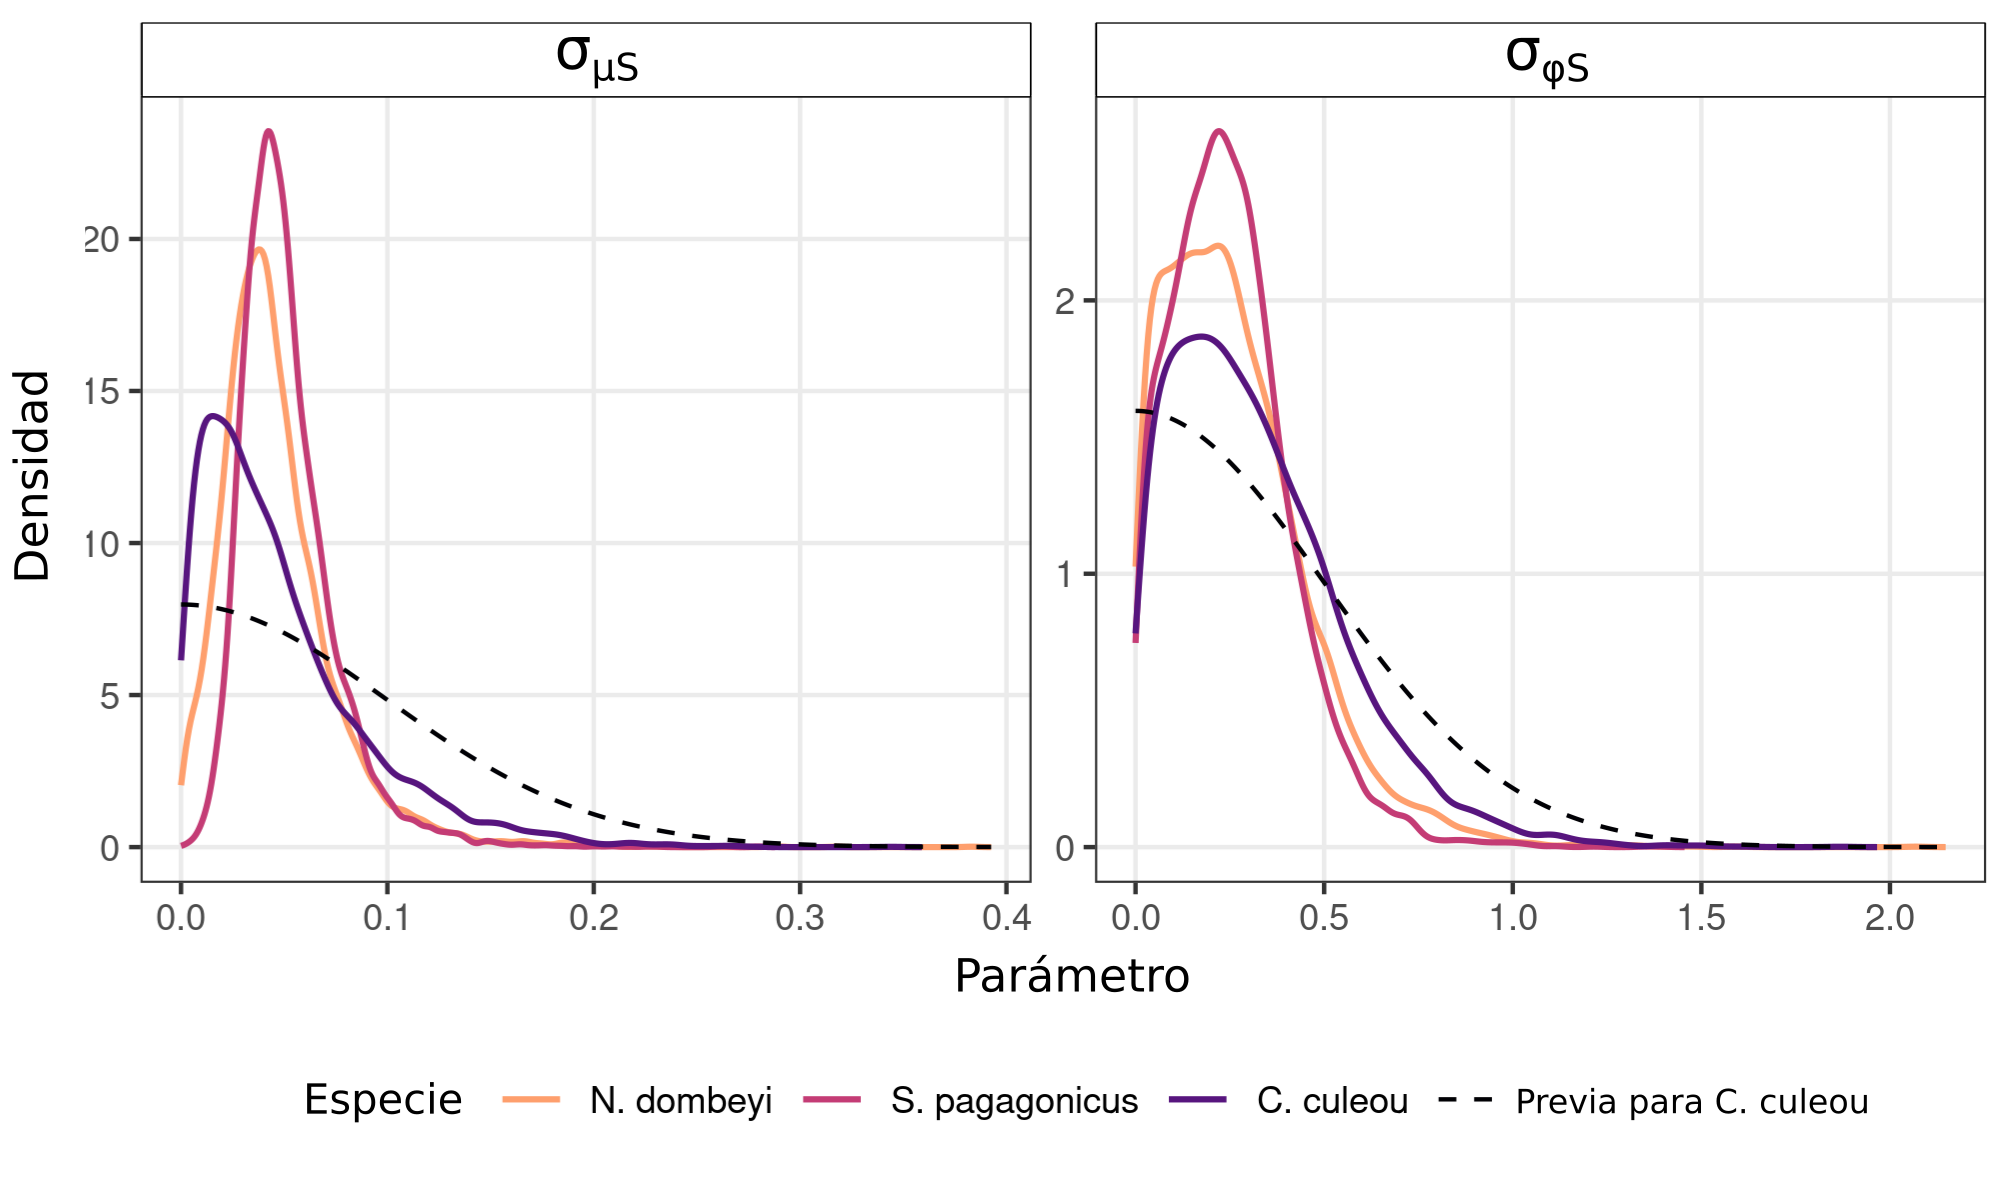
\includegraphics{figuras/cap2/S17) priors.png}
\end{center}
\end{figure}

Para todos los modelos de humedad de combustible, corrimos 10 cadenas durante 1000 iteraciones después de la fase de calentamiento (1500 para la mezcla de combustibles vivos, 2500 para las varillas de combustible de 1 h), y el número de iteraciones de calentamiento por cadena varió según el tipo de combustible: 12000 para \textit{C. culeou}, 1500 para la mezcla de combustibles vivos y 1000 para los demás tipos de combustible. El calentamiento más largo para algunos modelos fue necesario para evitar transiciones divergentes durante la fase de muestreo, y el mayor número de muestras en algunos tipos de combustible fue necesario para alcanzar un tamaño efectivo de muestra alto. A lo largo de todos los modelos de humedad de combustible y parámetros (incluyendo cantidades derivadas calculadas en Stan), el valor máximo de $\hat{\text{R}}$ fue 1.0086, lo que indica convergencia, y el tamaño efectivo de muestra más pequeño fue 826.7.
\newpage{\ }
\cleardoublepage

\chapter{Apéndice Capítulo 3}\label{append_03}

\section{Variación del tipo de vegetación en función de variables ambientales}\label{append:veg}

Para entender mejor cómo el fuego se ve afectado por la interacción entre el tipo de vegetación y los factores físicos y humanos (variables ambientales), realizamos un análisis cuantitativo de cómo el tipo de vegetación responde a la topografía, la precipitación y la distancia a poblados y caminos. Basamos este análisis en el mapa de vegetación de la Ecorregión Valdiviana de WWF \citep{lara_vegetacion_1999}, reclasificado en 8 categorías siguiendo a \citet{kitzberger_projections_2022}, que se muestran en la figura~\ref{fig:cap3-01}B: bosque húmedo (clases originales 01, 03, 05, 06, 07 y 11), bosque subalpino (clases 08 y 02), bosque seco (clase 04), matorral (clase 09), pastizal (clases 13 y 14), plantaciones (clase 17) y praderas antrópicas (clases 16 y 18) y la clase no quemable (15, 19, 20, 21 y 22), que fue excluida de nuestro análisis. La clase 02 en el mapa original comprendía principalmente bosques subalpinos dominados por \textit{N. pumilio}, con presencia de \textit{Araucaria araucana}, pero \citet{lara_vegetacion_1999} etiquetaron esta comunidad como bosque de \textit{A. araucana}. La clasificamos como bosques subalpinos porque la vegetación dominante es la más importante para la ocurrencia del fuego. Usamos la misma base de datos que en el análisis de patrones espaciales de fuego, que consistió en datos ambientales muestreados en 8278 puntos en el área quemable (ver la Sección~\ref{cap3:spat-analyses}). Se ajustaron Modelos Aditivos Generalizados (GAMs) asumiendo una distribución categórica del tipo de vegetación, con variables topográficas, precipitación y distancia a poblados y caminos como predictoras. Se utilizaron modelos univariados y múltiples (es decir, incluyendo sólo uno o todos las predictoras a la vez). En todos los casos modelamos el efecto de las predictoras con splines cúbicos de tres funciones de base (\texttt{k = 4} en \texttt{mgcv}), pero para la orientación especificamos \textit{splines} cúbicas cíclicas. No incluimos el NDVI como predictora porque no es una causa del tipo de vegetación, sino más bien una consecuencia. Al igual que con los modelos de probabilidad de quema, no analizamos la temperatura porque estaba altamente correlacionada con la altitud ($\rho = - 0.77$), y esta última tenía una resolución mucho más fina ($\approx$~930 m frente a 30 m). En estos modelos no se incluyeron las clases de vegetación plantación y pradera antrópica debido a su escasa abundancia en el paisaje.

Los modelos univariados permiten evaluar el efecto global de una predictora sobre la vegetación a escala regional; mientras que el modelo multivariado permite una descripción a escala más fina de cómo afectan las predictoras a la vegetación, dado que se incluyen las predictoras más importantes a escala regional. Esto se debe a que en el modelo multivariado los efectos parciales pueden evaluarse en los valores de las predictoras más importantes donde se da cada tipo de vegetación. Por ejemplo, podemos evaluar las preferencias topográficas de los pastizales en el rango de baja altitud y precipitación, donde son más abundantes. Además, el modelo múltiple permite identificar cuáles son las predictoras más relevantes cuando están correlacionadas (siempre que las correlaciones no sean demasiado altas). 

Los modelos univariados mostraron que el tipo de vegetación variaba principalmente en función de la altitud, la precipitación y la pendiente (Fig.~\ref{fig:cap3-S01}, Tabla~\ref{tab:cap3-S01}). A lo largo del gradiente altitudinal, los bosques secos ocuparon la porción más baja junto con los pastizales ($<$ 500 m s.n.m.), que se extendieron hasta la porción media del gradiente. Los matorrales y bosques húmedos fueron más abundantes entre los 500 y 1200 m s.n.m., y los bosques subalpinos dominaron por encima de los 1200 m s.n.m. y hasta el límite arbóreo (\textit{treeline}; Fig.~\ref{fig:cap3-S01}A). Las áreas con pendientes por debajo de 10° estaban dominadas por matorrales y pastizales; en pendientes más pronunciadas, los bosques subalpinos eran el tipo dominante, y los bosques húmedos eran más abundantes en áreas de pendientes intermedias (10 a 40°; Fig.~\ref{fig:cap3-S01}B). A lo largo del gradiente de precipitación, los bosques húmedos ocuparon el extremo más húmedo, seguidos por los matorrales y los bosques subalpinos, y después por los bosques secos. Finalmente, las estepas ocuparon la porción más seca del gradiente (Fig.~\ref{fig:cap3-S01}E). La orientación sólo mostró influencia en los bosques subalpinos, que tendían a localizarse en las laderas sureste, donde los pastizales y matorrales eran menos abundantes (Fig.~\ref{fig:cap3-S01}C). Los matorrales, bosques húmedos y secos fueron más abundantes en posición topográfica baja, mientras que los bosques subalpinos dominaron las laderas medias y altas, con los pastizales asociados a la posición topográfica alta (Fig.~\ref{fig:cap3-S01}D). En áreas cercanas a poblados y caminos los tipos más abundantes fueron pastizales, matorrales y bosques secos; los bosques subalpinos mostraron la mayor cobertura esperada a distancia intermedia, y los bosques húmedos, a gran distancia (Fig.~\ref{fig:cap3-S01}F y \ref{fig:cap3-S01}G).

En el modelo de regresión múltiple, en el que se incluyeron todas las predictoras a la vez, los efectos de la altitud y la precipitación permanecieron inalterados, los efectos de la orientación fueron más claros, y el resto de las predictoras mostraron efectos más leves (Fig.~\ref{fig:cap3-S02}). Una vez considerada la altitud, la pendiente y la posición topográfica perdieron importancia, ya que presentaban una correlación positiva con la altitud (Fig.~\ref{fig:cap3-S04}). En este modelo, los bosques secos y los matorrales presentaron mayor cobertura en posición topográfica alta, y los bosques subalpinos mostraron una ligera preferencia por una posición topográfica baja (Fig.~\ref{fig:cap3-S02}D). Además, los bosques secos se vieron claramente asociados a pendientes pronunciadas (Fig.~\ref{fig:cap3-S02}B). En cuanto al orientación, los bosques subalpinos ocurrieron mayormente en las laderas del sur, mientras que los bosques húmedos, matorrales y pastizales, en laderas norte (Fig.~\ref{fig:cap3-S02}C). En cuanto a la distancia a poblados y caminos, los bosques húmedos mostraron su mayor cobertura esperada a corta distancia, lo opuesto al modelo univariado (Fig.~\ref{fig:cap3-S02}F y \ref{fig:cap3-S02}G). Esto ocurrió porque las áreas con mayor precipitación son también las más alejadas de poblados y caminos (Fig.~\ref{fig:cap3-S04}).


\begin{figure}[htbp]
    \centering
    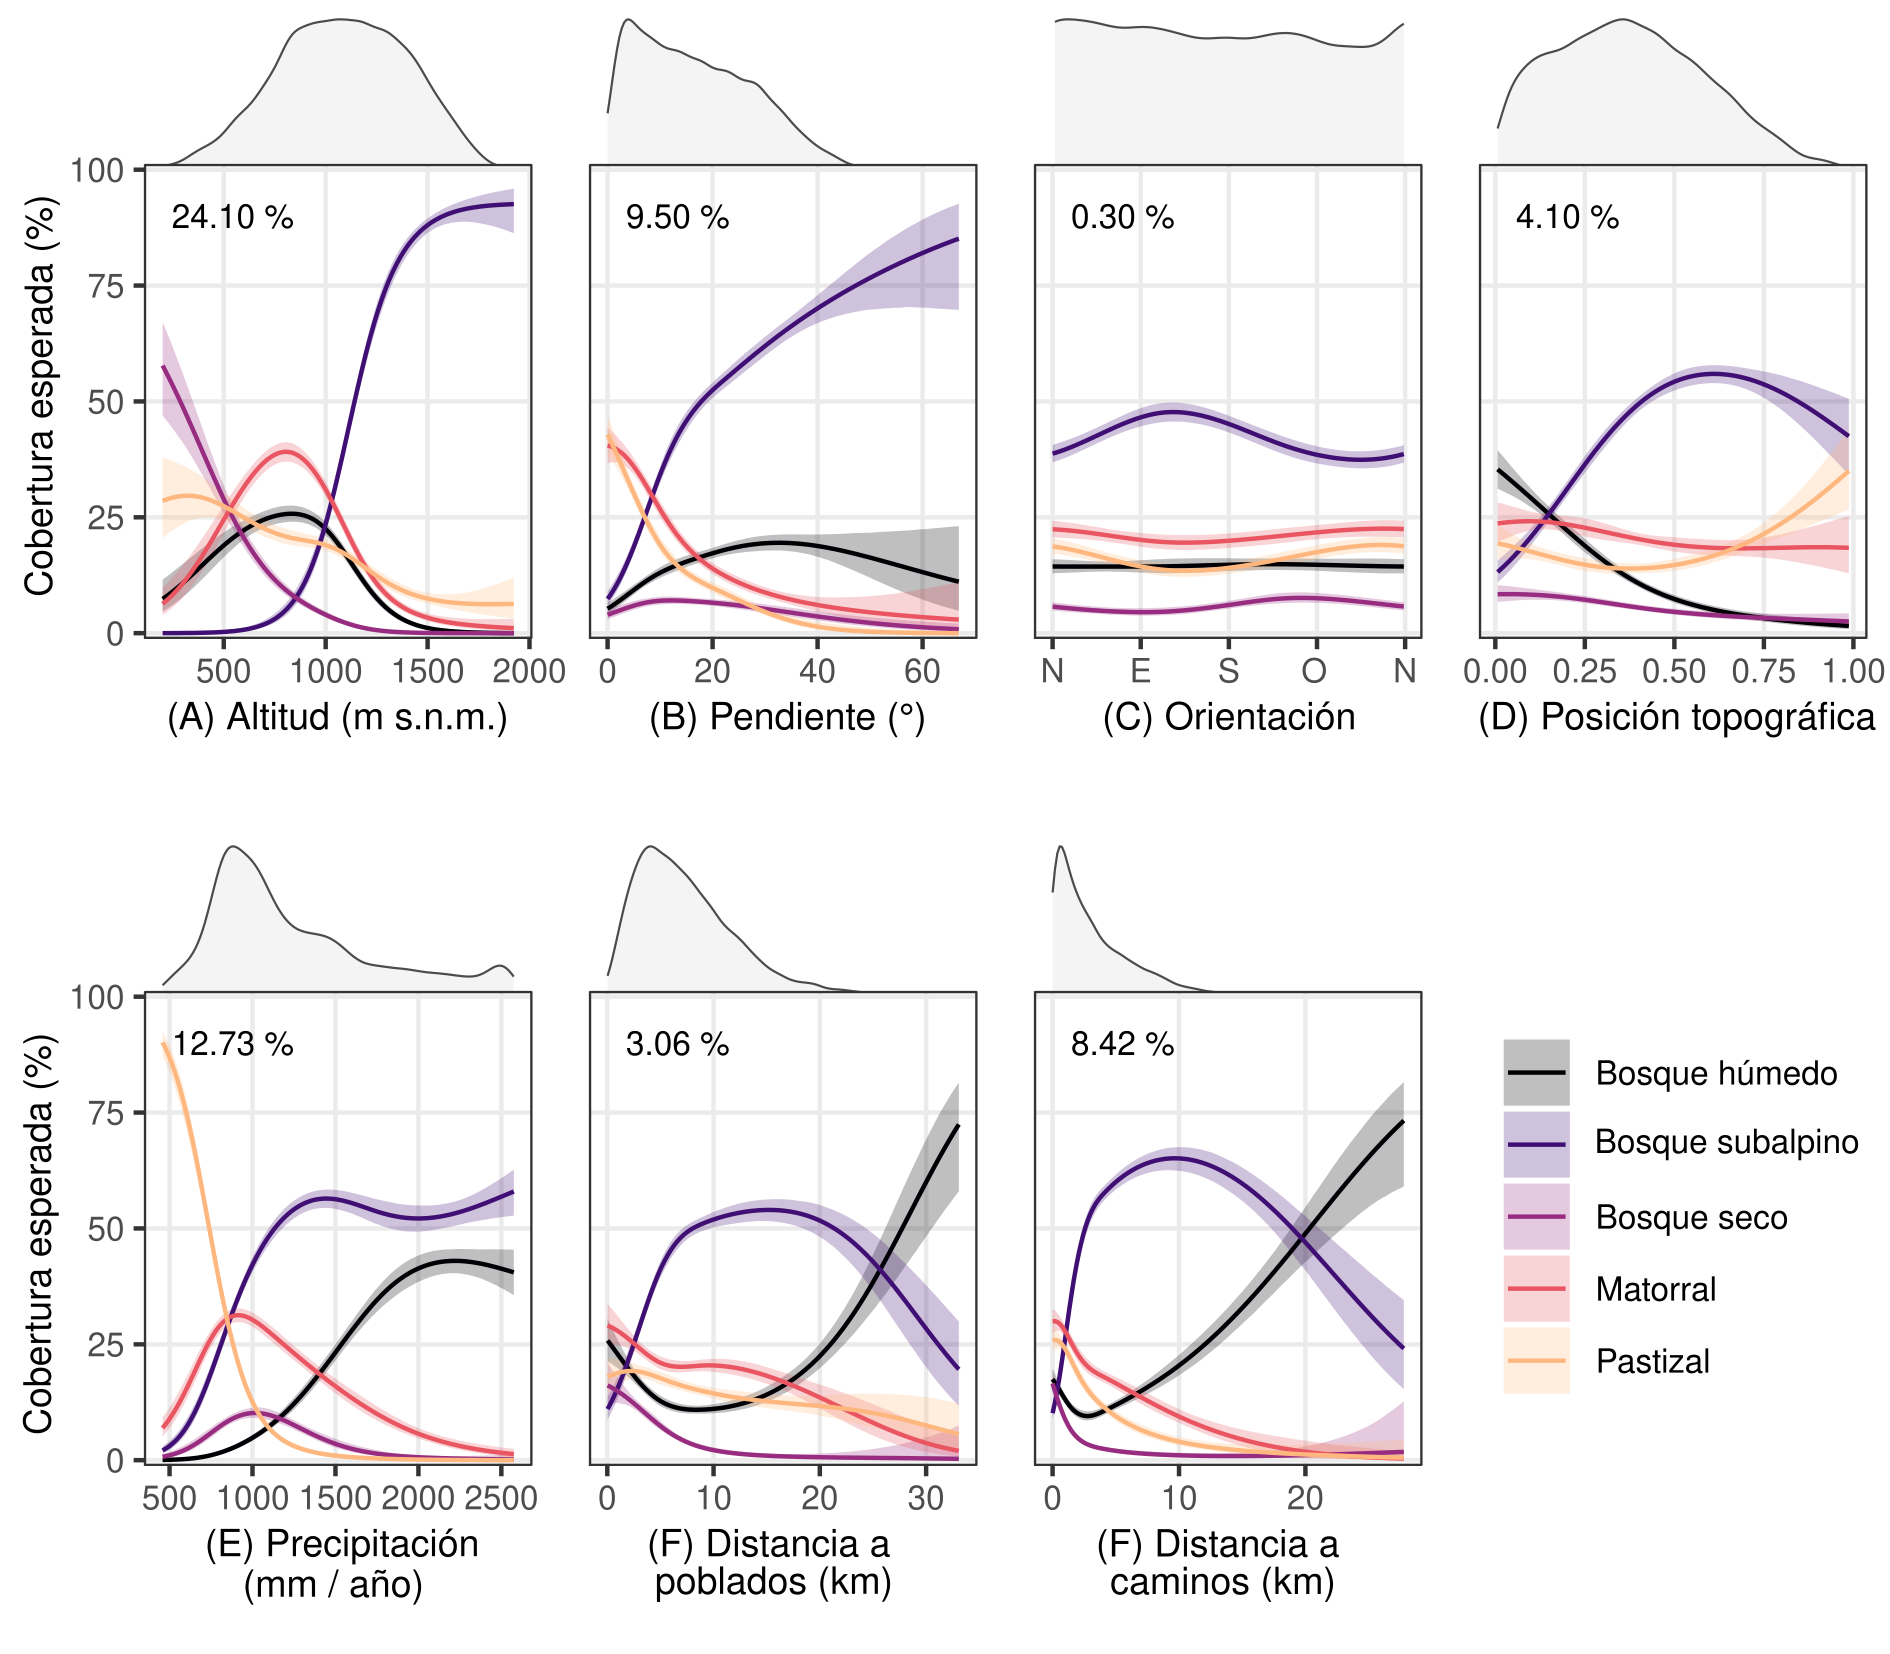
\includegraphics[width=16cm]{figuras/cap3/S01) vegetation_environment_marginal.png}
    \caption[Tipo de vegetación en función de variables ambientales, modelos univariados.]{Cobertura esperada (\%) de cada tipo de vegetación en función de las variables ambientales. Las líneas muestran la probabilidad estimada a partir de GAMs categóricos univariados con sus intervalos de confianza del 95 \%. Nótese que para cada valor de las predictoras todos los tipos suman 100 \%. Los números dentro de los paneles muestran el $\text{R}^2$ bayesiano de cada modelo, calculado como la media ponderada por abundancia del $\text{R}^2$ de cada tipo de vegetación, asumiendo una distribución Bernoulli de cada tipo. Las curvas grises arriba de los paneles muestran la distribución de cada variable predictora.} 
    \label{fig:cap3-S01}
\end{figure}


\begin{figure}
    \centering
    \rotatebox[origin=c]{90}{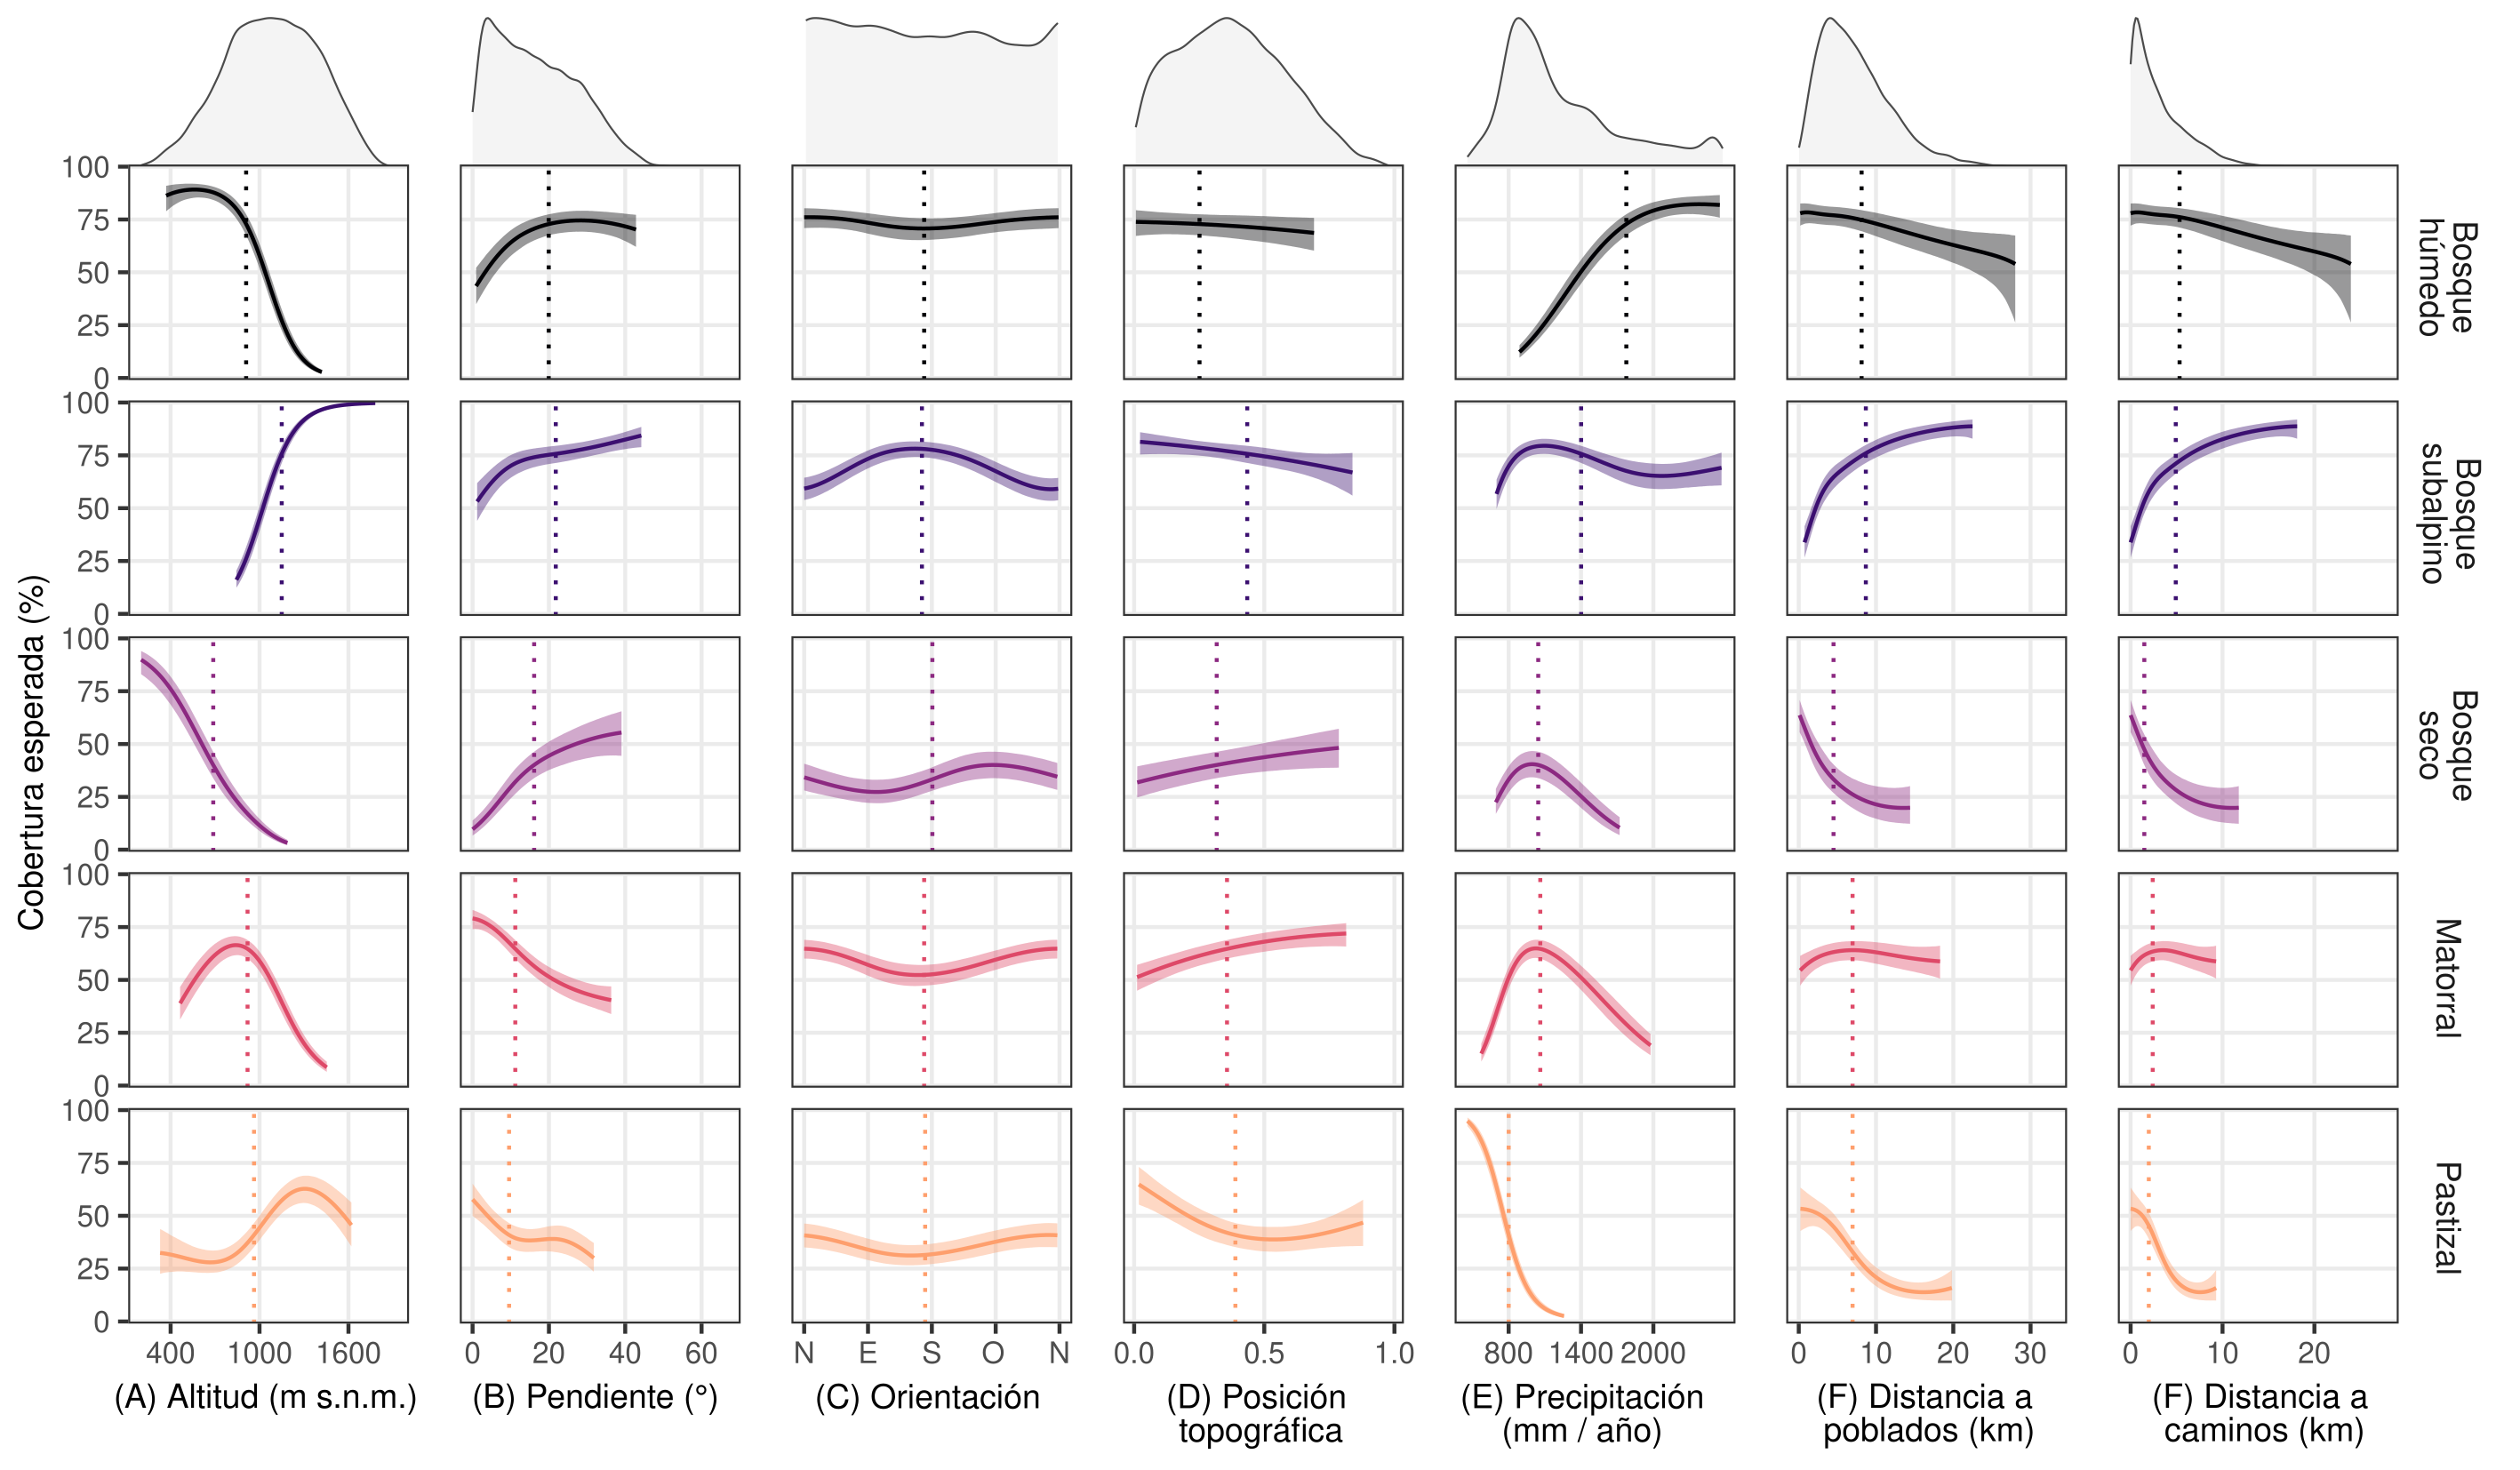
\includegraphics[width=0.95\textheight]{figuras/cap3/S02) vegetation_environment_conditional.png}}
    \caption[Tipo de vegetación en función de variables ambientales, modelo multivariado.]{(Leyenda en la página siguiente.)} 
    \label{fig:cap3-S02}
\end{figure}

% leyenda en la página siguiente
\begin{figure}[p]
  \contcaption{(en la página anterior). Cobertura esperada de cada tipo de vegetación en función de las variables ambientales, calculada a partir del GAM categórico de regresión múltiple. En cada panel se varía la predictora en el rango de cada tipo de vegetación, con el resto de las predictoras fijadas en la media correspondiente a cada tipo de vegetación (indicado con líneas verticales). En el caso del bosque subalpino, la altitud se fijó en 1150, en lugar de 1322 m s.n.m., para evitar que la cobertura esperada fuera cercana al 100 \%, ya que en este valor no se podían detectar efectos de otras predictoras. Las curvas grises arriba de los paneles muestran la distribución de cada variable predictora. Las predicciones abarcan el intervalo de mayor densidad del 98 \% de cada predictora en cada tipo de vegetación.} 
\end{figure}


\begin{table}
\caption[$\text{R}^2$ para los modelos de vegetación.]{$\text{R}^2$ (\%) para los modelos de tipo de vegetación, tanto univariado como multivariado (última inferior). El $\text{R}^2$ se calculó para cada tipo por separado como el $\text{R}^2$ bayesiano para una variable con distribución Bernoulli. En la figura~\ref{fig:cap3-S01} se muestra la media de $\text{R}^2$ ponderada por abundancia para cada modelo univariado. Las predicciones del modelo de regresión múltiple se muestran en la figura~\ref{fig:cap3-S02}.}
\label{tab:cap3-S01}
\resizebox{16cm}{!}{%
\begin{tabular}{l|ccccc}
\toprule
Variable & Bosque húmedo & Bosque subalpino & Bosque seco & Matorral & Pastizal \\
\midrule
Altitud & 7.16 & 46.11 & 13.98 & 10.79 & 2.75\\
Pendiente & 1.46 & 14.34 & 0.19 & 7.79 & 9.72\\
Orientación & 0.00 & 0.53 & 0.21 & 0.07 & 0.28\\
Posición topográfica & 6.76 & 6.95 & 0.53 & 0.28 & 0.55\\
Precipitación & 17.61 & 8.84 & 2.30 & 5.86 & 31.31\\
Distancia a poblados & 2.44 & 5.41 & 3.41 & 0.69 & 0.44\\
Distancia a caminos & 4.20 & 14.44 & 4.18 & 3.28 & 4.73\\
\midrule
Regresión múltiple & 43.04 & 56.77 & 27.72 & 24.87 & 40.67\\
\bottomrule
\end{tabular}
}
\end{table}

Estos patrones indican que a pesar de que las variables ambientales están asociadas al tipo de vegetación, la relación no es demasiado estrecha, lo que permite separar aproximadamente los efectos del tipo de vegetación y las variables ambientales sobre el fuego. Esto es posible por dos razones. La primera es que con un considerable solapamiento entre tipos de vegetación a lo largo de gradientes ambientales podemos comparar la probabilidad de quema estimada entre tipos de vegetación bajo las mismas condiciones ambientales, representando efectos más puros de la vegetación sobre el fuego. Esto permite comparar cómo cambia el patrón de probabilidad de quema entre tipos de vegetación si se controlan o no las variables ambientales (Fig.~\ref{fig:cap3-06}C vs. \ref{fig:cap3-06}A, respectivamente). La segunda razón es la gran variación ambiental dentro de los tipos de vegetación (ver densidades rosas en Fig.~\ref{fig:cap3-04} y \ref{fig:cap3-05}, filas 2 a 6), que permiten estimar el efecto de las variables ambientales dentro de los tipos de vegetación, para compararlo con su efecto global, que ignora el tipo de vegetación (primera fila en Fig.~\ref{fig:cap3-04} y \ref{fig:cap3-05}). Estos aspectos de los datos están representados por los modelos que predicen el tipo de vegetación (Fig.~\ref{fig:cap3-S01} y \ref{fig:cap3-S02}) y por la distribución de las variables ambientales dentro de los tipos de vegetación (Fig.~\ref{fig:cap3-04} y \ref{fig:cap3-05}, filas 2 a 6). Pero a su vez, puede notarse de forma más compacta identificando los tipos de vegetación en un ordenamiento de los puntos muestreados según las variables ambientales (Fig.~\ref{fig:cap3-S03}). Las regiones de mayor densidad para las coordenadas del Análisis de Componentes Principales por tipo de vegetación muestran un solapamiento considerable, y también reflejan una notable variación ambiental dentro de cada tipo.

\begin{figure}[htbp]
    \centering
    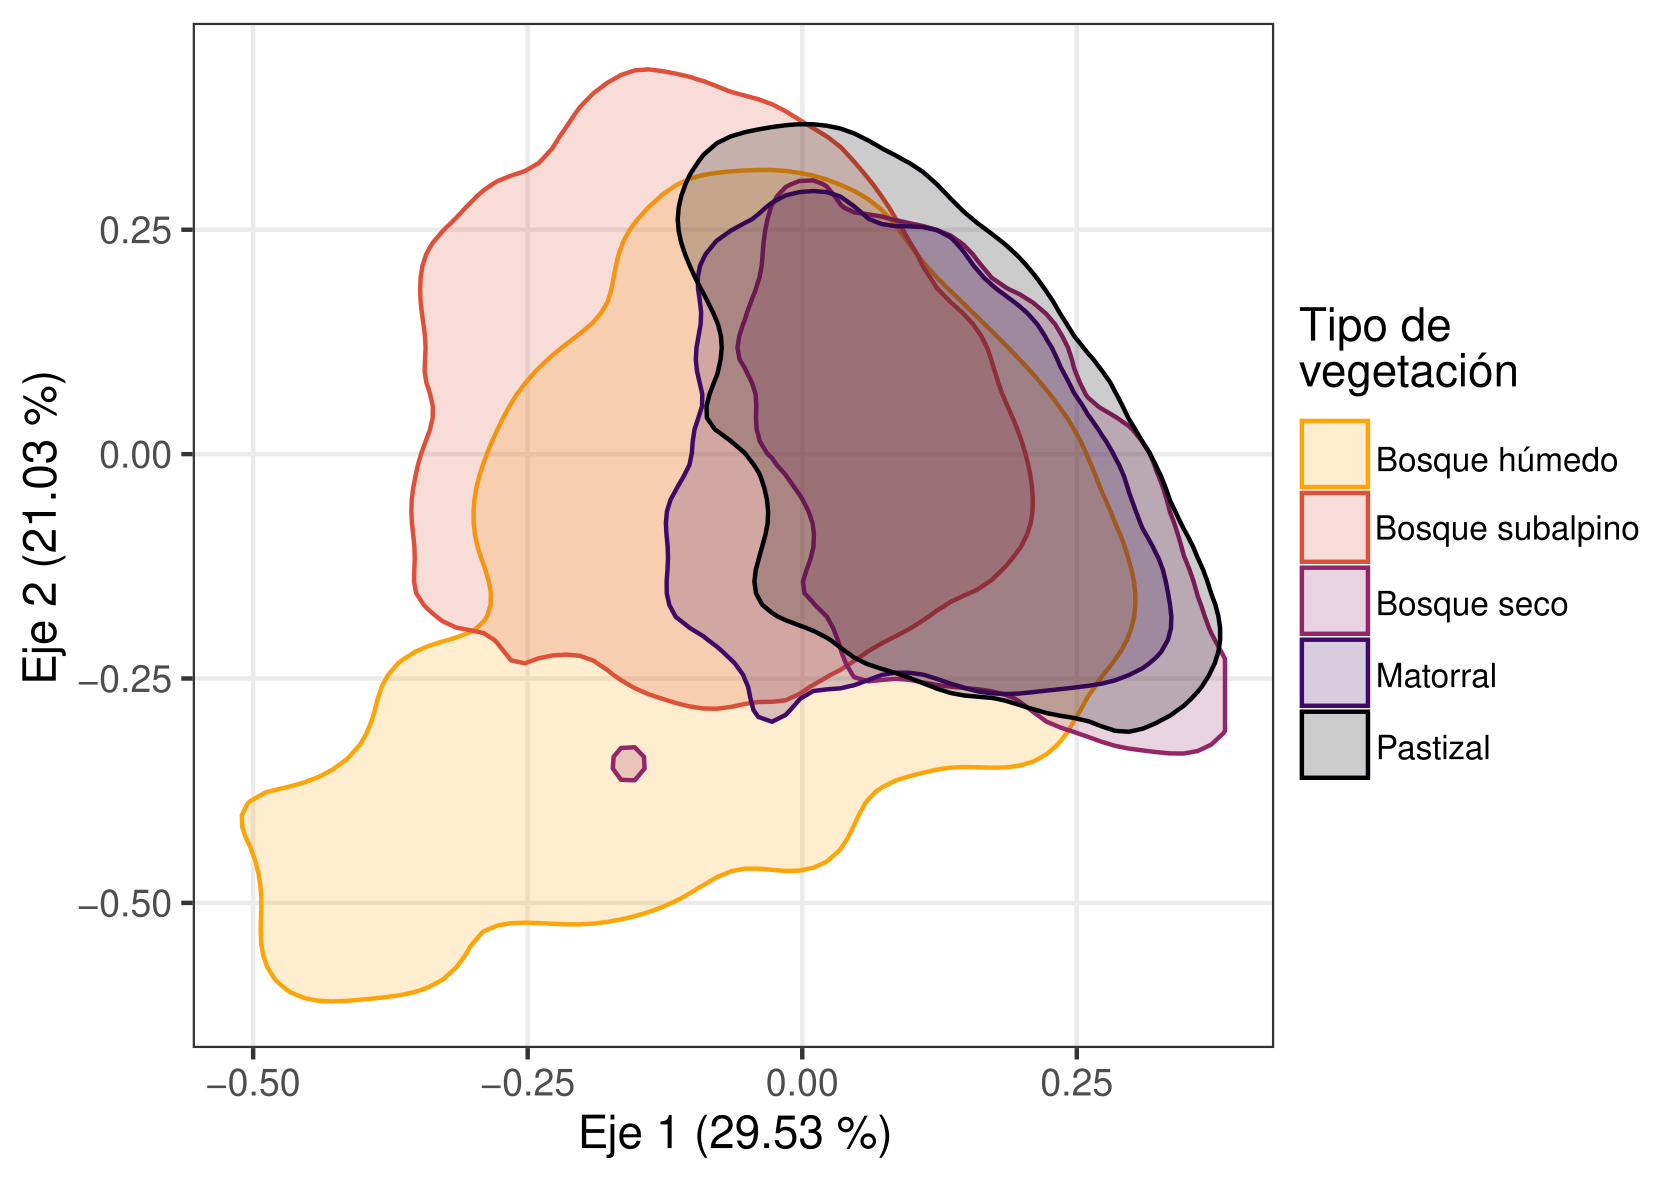
\includegraphics[width=14cm]{figuras/cap3/S03) ordination.png}
    \caption[Ubicación de tipos de vegetación en un ordenamiento basado en variables ambientales.]{Primeros dos ejes de un Análisis de Componentes Principales (ACP) realizado con las 7 predictoras ambientales: altitud, pendiente, orientación [transformado a su componente norte como cos(orientación)], posición topográfica, precipitación, distancia a poblados y distancia a caminos. Como teníamos demasiados puntos de datos para visualizarlos correctamente (N = 8018), sólo mostramos las regiones de mayor densidad del 90 \% para las coordenadas del ACP de cada tipo de vegetación. Los datos se agruparon por tipo de vegetación luego de correr el ACP. Los porcentajes indican la parte de la varianza explicada por cada eje.} 
    \label{fig:cap3-S03}
\end{figure}

\begin{figure}[htbp]
    \centering
    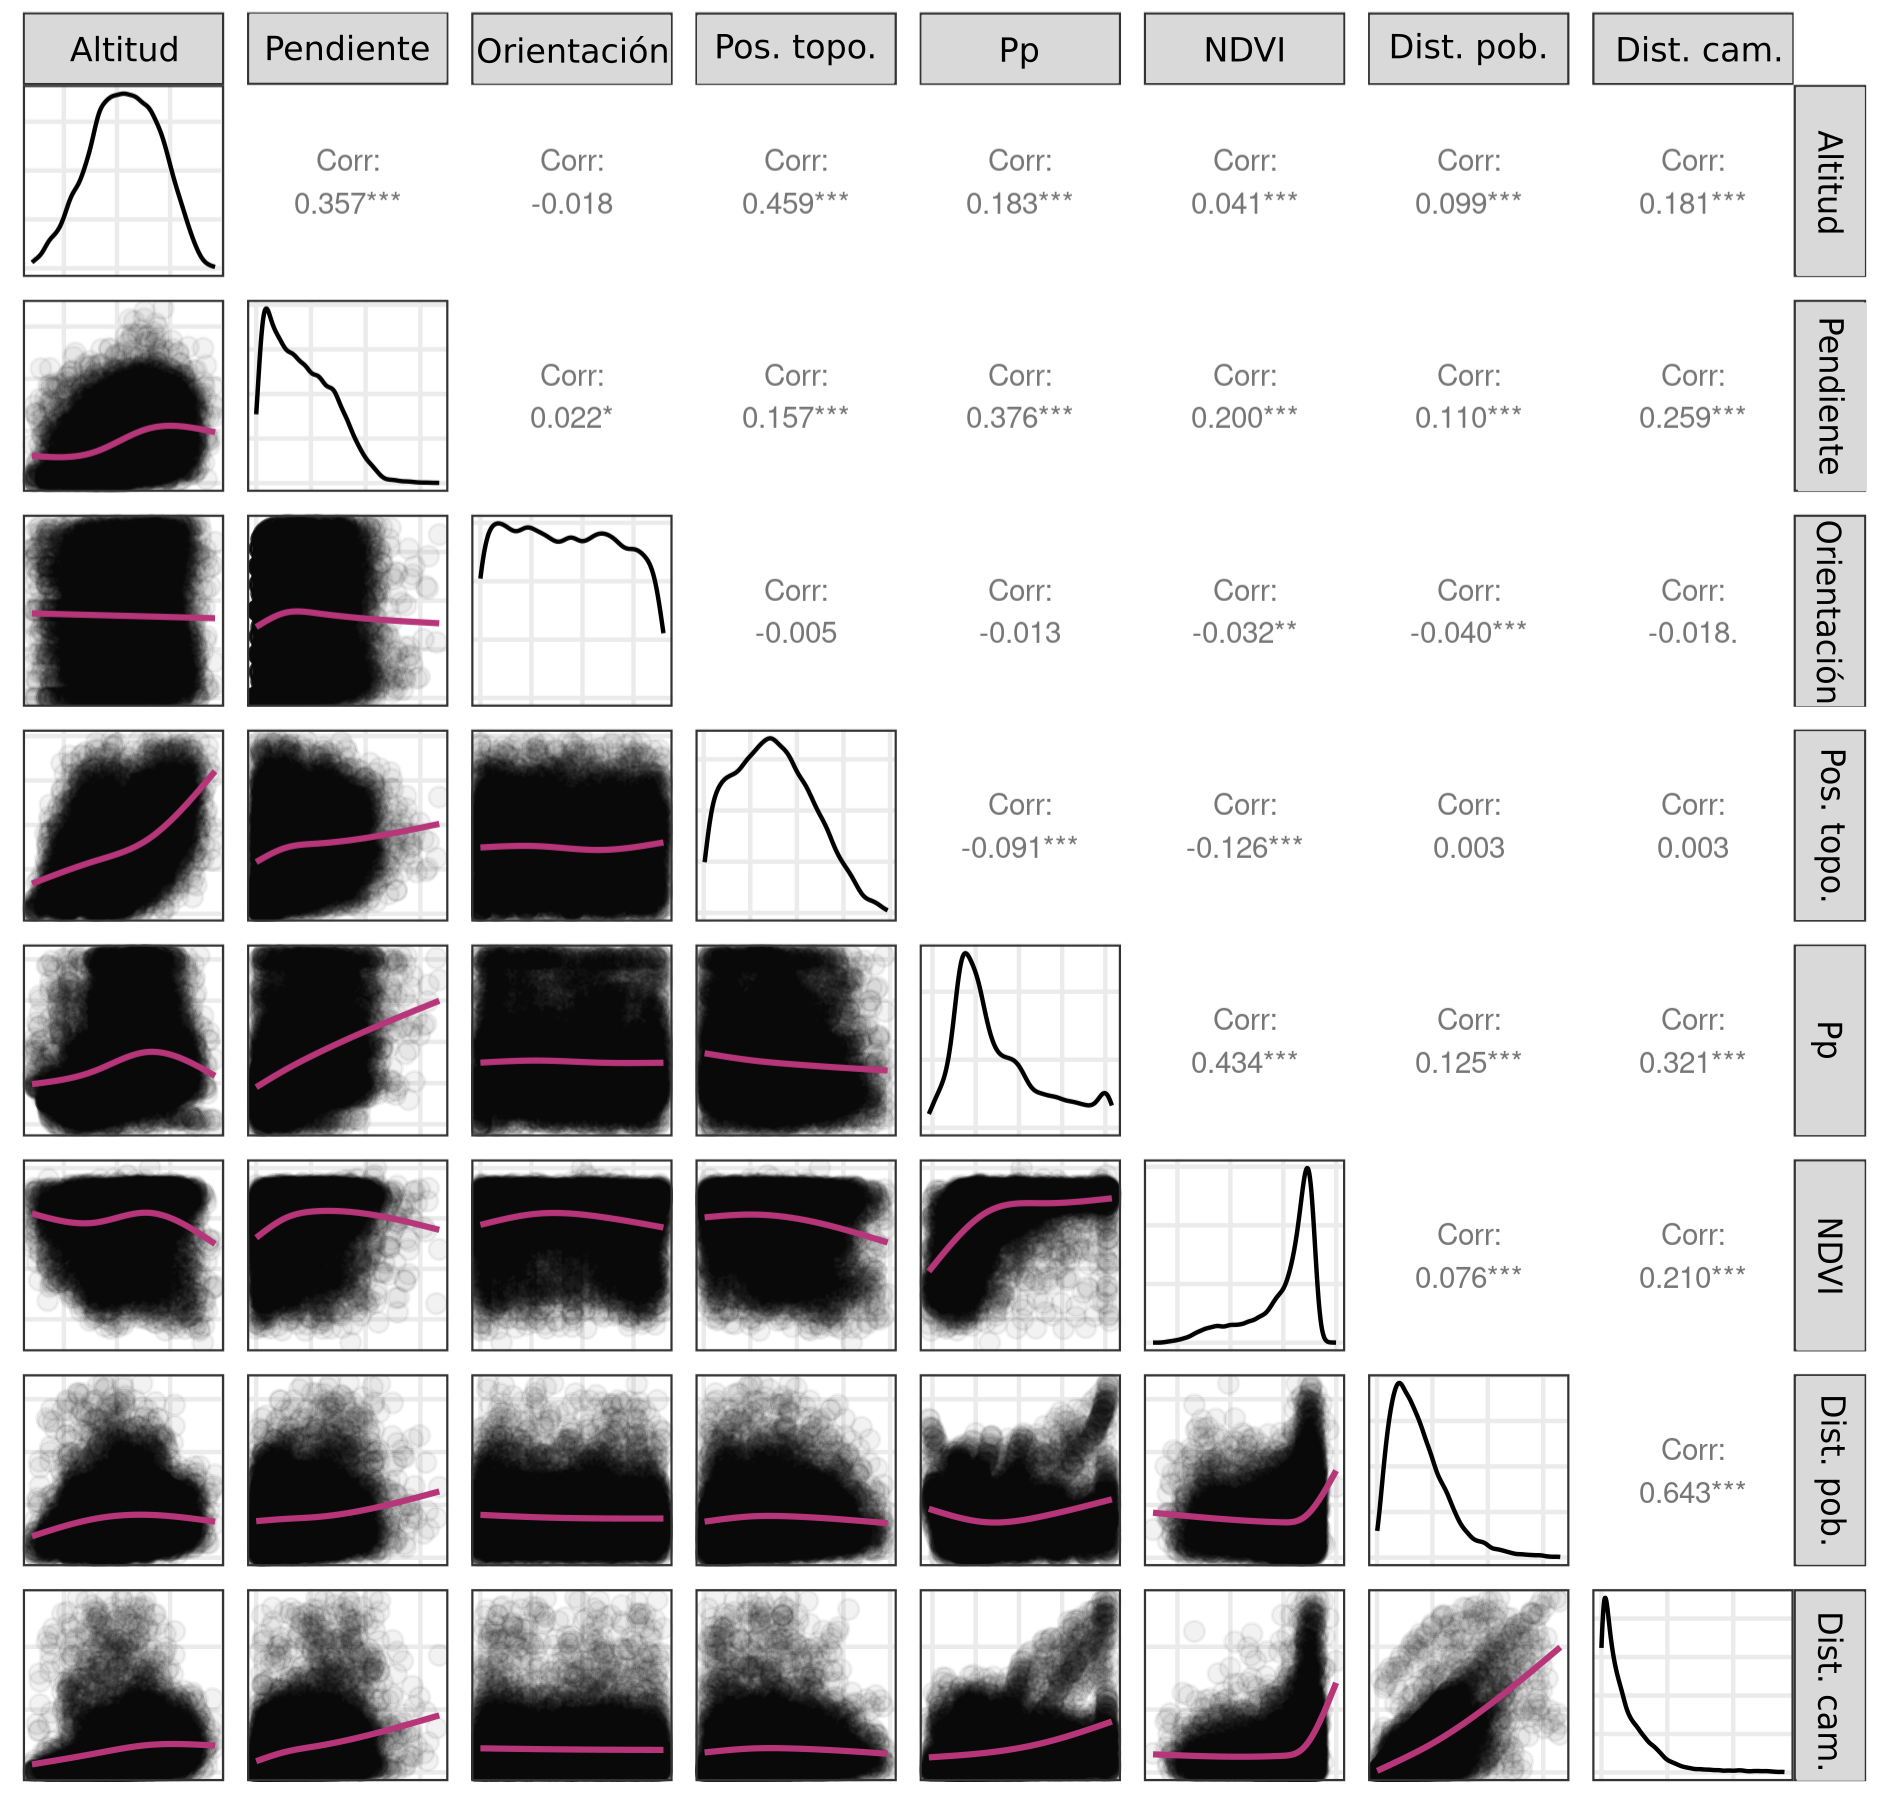
\includegraphics[width=16cm]{figuras/cap3/S04) correlations_env.png}
    \caption[Correlación entre predictoras ambientales.]{Diagramas de dispersión de todas las predictoras de probabilidad de quema, utilizando los 8228 puntos muestreados en el área quemable. Las líneas muestran el ajuste de un GAM con \textit{splines} cúbicas de tres funciones base (\texttt{k = 4} en \texttt{mgcv}), asumiendo una distribución normal de la respuesta. En los paneles diagonales se muestra la distribución de cada variable, y los números de los paneles superiores muestran el coeficiente de correlación de Pearson. Abreviaturas: Pos. topo: posición topográfica; Pp: precipitación; Dist. pob.: distancia a poblados; Dist. cam.: distancia a caminos.} 
    \label{fig:cap3-S04}
\end{figure}

\FloatBarrier

\section{Mapeo de incendios}\label{append:mapeo}

El procedimiento de mapeo fue semiautomático: en primer lugar, produjimos polígonos de áreas quemadas con un enfoque automático en Google Earth Engine \citep{gorelick_google_2017} utilizando índices de quema y de vegetación (NDVI: Índice de Vegetación de Diferencia Normalizada y NBR: Razón de Quema Normalizado), y luego editamos manualmente los polígonos de incendios para corregir errores (Fig.~\ref{fig:cap3-S05}). El enfoque automático resultó confiable para detectar la ubicación de los incendios, pero como la señal de quema (reducciones de NBR y NDVI) permanece al menos un año después del incendio, muchos incendios o partes de ellos se asignaban incorrectamente a años adyacentes. Además, las zonas quemadas muestran propiedades espectrales similares a las zonas afectadas por otros disturbios, como talas y defoliaciones por insectos, lo que hace que el procedimiento automático genere cierto grado de error de comisión. La revisión manual permitió superar estos problemas. La base de datos está disponible públicamente en GitHub (\url{https://github.com/barberaivan/patagonian_fires.git}).

Realizamos el mapeo de incendios en pasos anuales, pero como la mayor parte de ellos ocurren entre diciembre y marzo en nuestra área de estudio, consideramos los años corriendo de julio a junio, etiquetándolos con el año del mes final para simplificar. Por ejemplo, un incendio ocurrido en octubre de 1998 se asigna al año de fuego 1999.

\begin{figure}[htbp]
    \centering
    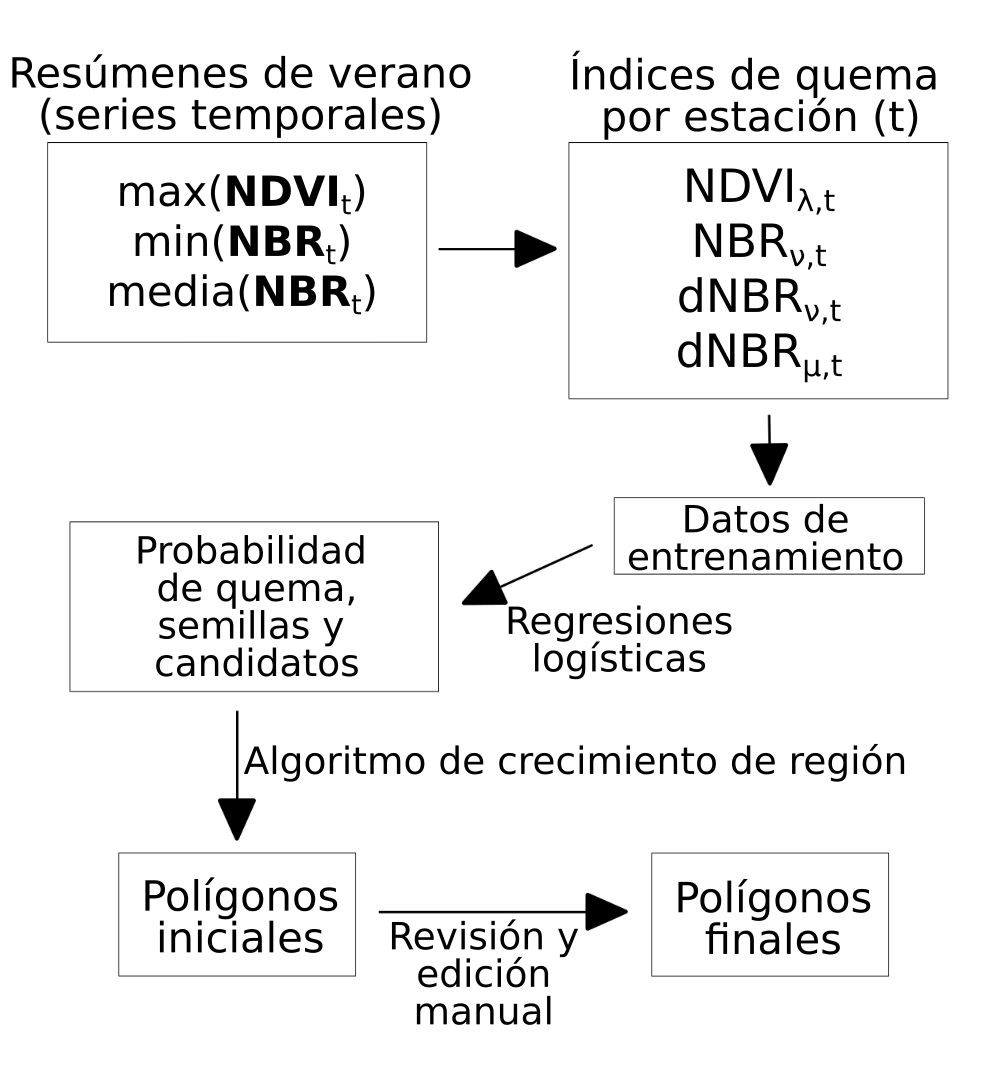
\includegraphics[width=9cm]{figuras/cap3/S05) mapping_algorithm.png}
    \caption[Algoritmo de mapeo de incendios.]{Esquema del algoritmo de mapeo de incendios. La mayor parte del procedimiento se llevó a cabo en Google Earth Engine \citep{gorelick_google_2017}, mientras que las regresiones logísticas se ajustaron en R \citep{R}, y para la revisión y edición manual utilizamos ambos software combinados con QGIS \citep{qgis326}. Los índices de vegetación brutos utilizados fueron el NDVI y el NBR; los índices de quema por estación se definen en la Ecuación~\ref{eq:cap3-burnindex}. El sufijo $t$ indica cada año, incluyendo imágenes sólo de diciembre a abril y tomando la etiqueta del año final.} 
    \label{fig:cap3-S05}
\end{figure}

\subsection{Fase automática}

La etapa de mapeo automático fue similar a la descrita por \citet{long2019}, basada en un algoritmo de crecimiento de región: para cada año desde 1999 hasta 2022 (incluido) definimos por separado los píxeles con alta probabilidad de ser quemados, llamados semillas, y los píxeles con probabilidad baja o media, llamados candidatos. El algoritmo de crecimiento de región genera grupos de píxeles quemados a partir de las semillas, se y extiende hasta incluir todos los píxeles candidatos vecinos (8 píxeles) (algoritmo SNIC en Google Earth Engine; \citealt{AchantaSNIC}). La probabilidad de quema a nivel de píxel utilizada para definir semillas y candidatos se definió mediante tres modelos de regresión logística, utilizando índices basados en NDVI y NBR como predictoras (Fig.~\ref{fig:cap3-S06}A). Para cada año, calculamos el NDVI y el NBR a partir de todas las imágenes Landsat disponibles (producto de \textit{Surface Reflectance}, Colecciones 1 y 2) que intersecaban el área de estudio, tomadas entre diciembre y abril (incluidos), ya que este periodo tiene baja nubosidad. A partir de estas variables, calculamos cuatro índices derivados por año ($t$):

\begin{equation}
\begin{aligned}
    \text{NDVI}_{\lambda,t} &= \text{max}(\{\textbf{NDVI}_t, \textbf{NDVI}_{t-1}\}) \\  
    \text{dNBR}_{\mu,t} &= \text{media}(\textbf{NBR}_{t-1}) - \text{media}(\textbf{NBR}_{t+1})  \\
    \text{dNBR}_{\nu,t} &= \text{min}(\textbf{NBR}_{t-1}) - \text{min}(\textbf{NBR}_{t}) \\
    \text{NBR}_{\nu,t} &= \text{min}(\textbf{NBR}_t),
\end{aligned}
\label{eq:cap3-burnindex}
\end{equation}

\noindent y el máximo de los promedios de NDVI por año (verano):

\[
\text{NDVI}_{\lambda,\mu} = \text{max}[\{\text{media}(\textbf{NDVI}_{1999}), ..., \text{media}(\textbf{NDVI}_{2022})\}].
\]

\noindent Las variables en negrita representan vectores con todos los valores disponibles de los índices espectrales correspondientes entre diciembre y abril del año $t$, para cada píxel (ejemplo: para 1999 se utilizan imágenes de diciembre de 1998 a abril de 1999). A partir de los cuatro índices dinámicos (con el sufijo $t$) ajustamos tres regresiones logísticas para modelar la probabilidad de quema a nivel de píxel, definidas de la siguiente manera: 

\begin{equation}
\begin{aligned}
\text{logit}(p_{1,t}) &=  \alpha_1 + \beta_1 \ \text{dNBR}_{\mu,t}  +  \gamma_1 \ \text{NDVI}_{\lambda,t} + \delta_1 \ \text{dNBR}_{\mu,t} \ \text{NDVI}_{\lambda,t} \\
\text{logit}(p_{2,t}) &=  \alpha_2 + \beta_2 \ \text{dNBR}_{\nu,t}  +  \gamma_2 \ \text{NDVI}_{\lambda,t} + \delta_2 \ \text{dNBR}_{\nu,t} \ \text{NDVI}_{\lambda,t} \\
\text{logit}(p_{3,t}) &=  \alpha_3 + \beta_3 \ \text{NBR}_{\nu,t}  +  \gamma_3 \ \text{NDVI}_{\lambda,t} + \delta_3 \ \text{NBR}_{\nu,t} \ \text{NDVI}_{\lambda,t}.
\end{aligned}
\label{eq:cap3-burnmap}
\end{equation}

Ajustamos los modelos utilizando píxeles seleccionados en incendios conocidos y sus alrededores. Elegimos cinco incendios grandes bien documentados y seleccionamos visualmente aproximadamente 300 píxeles quemados y unos 300 no quemados por incendio, basándonos en la composición RGB de las imágenes Landsat poco después del fuego. Aprendimos a distinguir entre píxeles quemados y no quemados basándonos en el color de la imagen, evaluando si la serie temporal de NBR mostraba un descenso, e inspeccionando las imágenes de Google Earth en las que las zonas quemadas eran evidentes. El $\text{NDVI}_{\lambda,t}$ se incluyó para permitir que los umbrales basados en índices basados en NBR variaran en función de la productividad del píxel, ya que las áreas de baja productividad, como los pastizales, presentan una menor disminución de NBR cuando se queman comparado con las áreas de alta productividad, como los bosques (Fig.~\ref{fig:cap3-S06}A). Esta estrategia es similar al uso de índices de quema relativizados, como RdNBR \citep{miller2007rdNBR}, pero análisis exploratorios sugirieron que nuestro enfoque sería más preciso. También probamos Random Forests y Support Vector Machines, incluyendo como predictoras las bandas Landsat sin procesar y varios índices de vegetación. Como no encontramos mejoras en la precisión, optamos por los métodos de regresión más sencillos e interpretables.

Definimos las semillas como píxeles con probabilidad de quema $\ge 0.98$ para los tres modelos que también mostraban alta productividad ($\text{NDVI}_{\lambda,\mu} \ge 0.7$) o baja altitud ($<$ 1300 m s.n.m.). Con estas restricciones adicionales se evitaron falsos positivos que aparecían en zonas altoandinas, frecuentemente cubiertas de nieve. Los candidatos se definieron por separado en función de la productividad de los píxeles:

\begin{enumerate}
    \item $p_1 \ge 0.20$ si $\text{NDVI}_{\lambda,t} > 0.5$, y
    \item $\{p_2, p_3\} \ge 0.25$ si $\text{NDVI}_{\lambda,t} \le 0.7$. 
\end{enumerate}    

\noindent De este modo, los índices utilizados para definir la probabilidad de quema de los píxeles de baja productividad ($\text{NDVI}_{\lambda,t} \le 0.7$) no utilizan el NBR del año siguiente ($t+1$), lo que resultaba conveniente porque los pastizales se recuperan rápidamente, por lo que $p_1$ no detecta correctamente los pastizales quemados. Por el contrario, las zonas boscosas $\text{NDVI}_{\lambda,t} > 0.5$ muestran una disminución prolongada del NBR cuando se queman, por lo que el uso de $p_1$ es mejor para clasificar esos píxeles. La figura~\ref{fig:cap3-S06}B muestra las tasas de error por comisión y omisión de cada modelo.
A los polígonos de incendios del mismo año se les asignó el mismo ID de incendio si estaban separados por menos de 85 m (más cerca que dos píxeles diagonales de 30 m).

\begin{figure}[htbp]
    \centering
    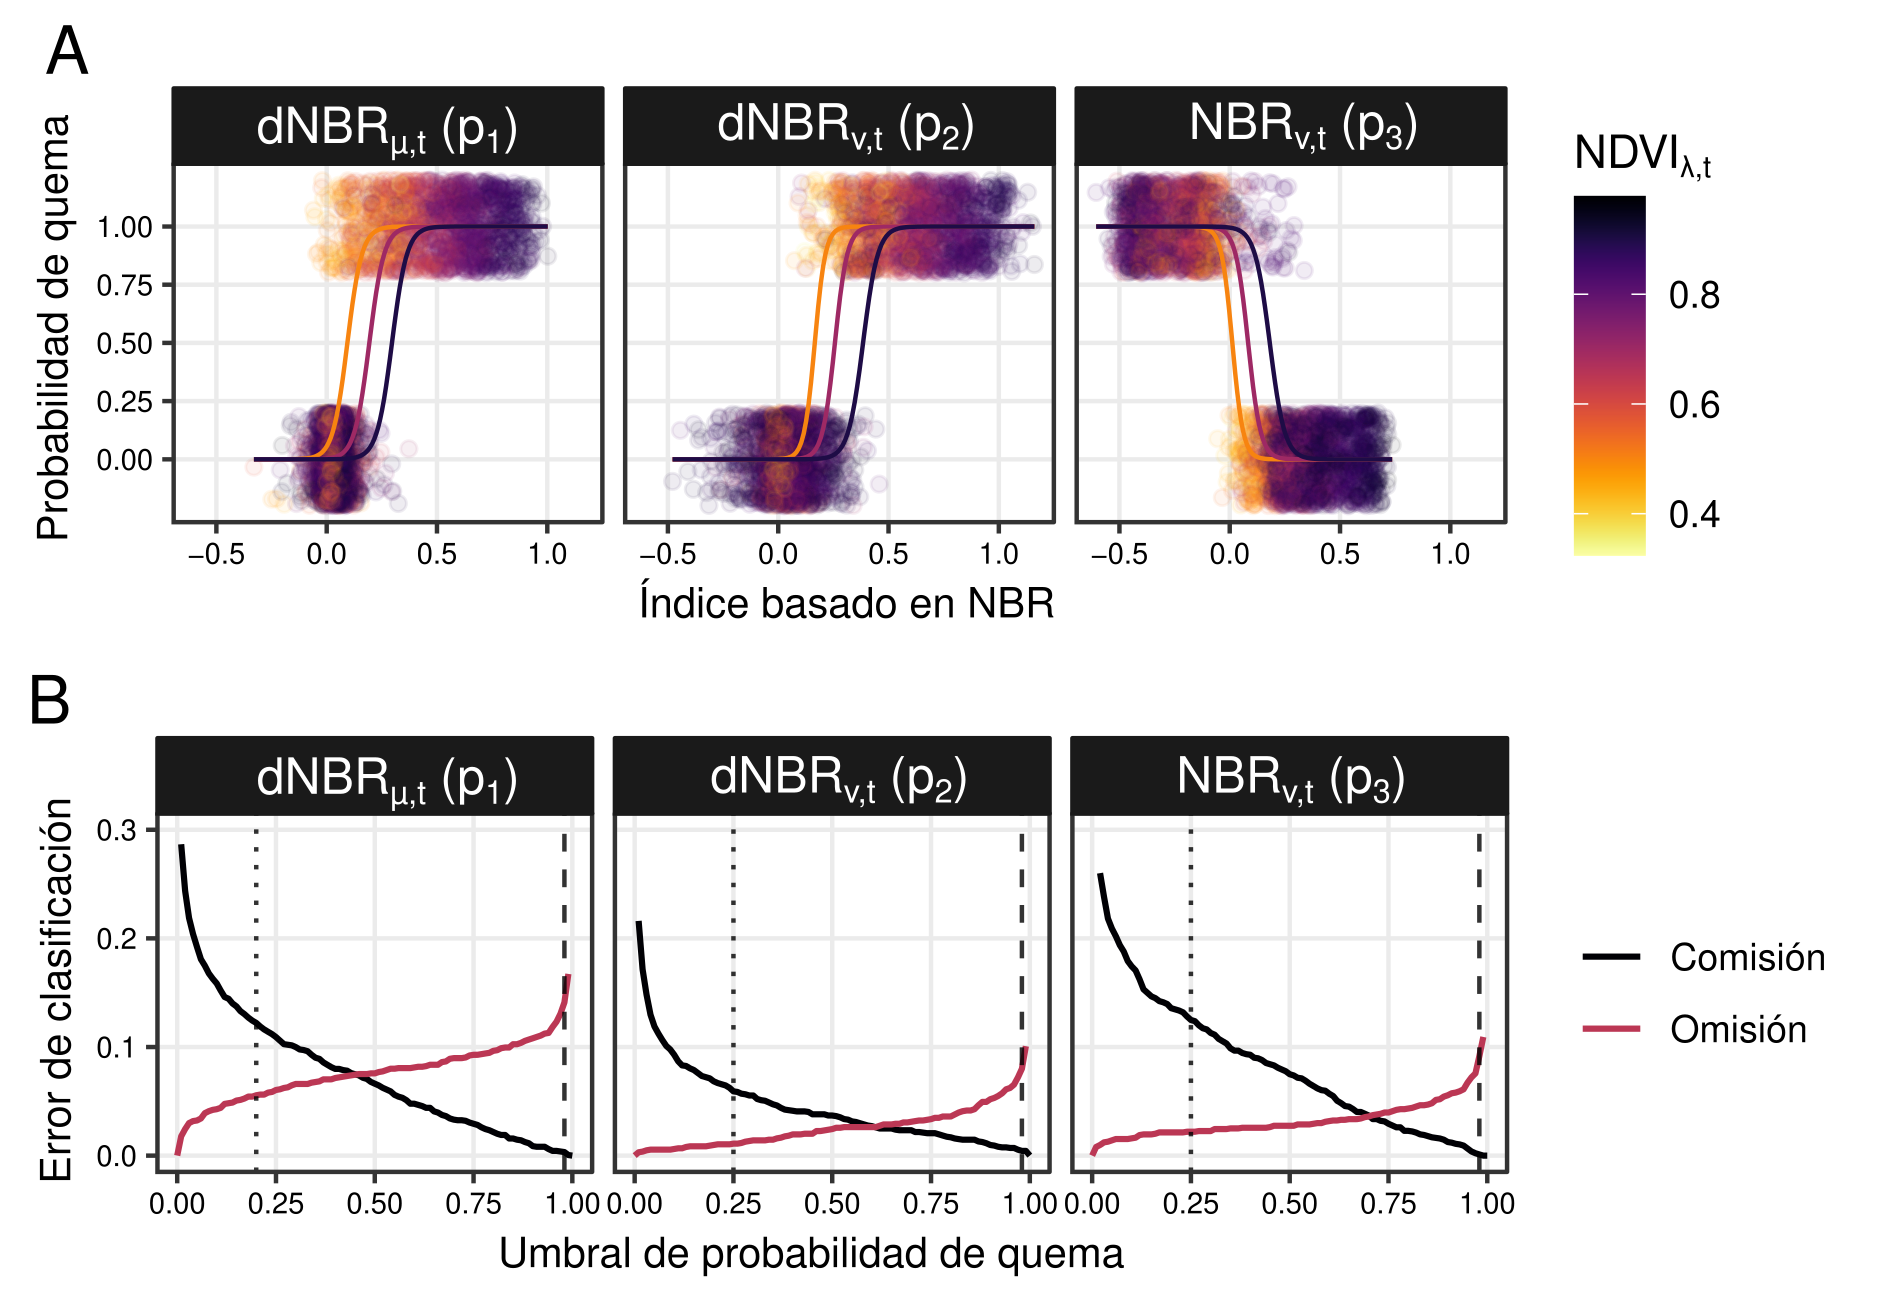
\includegraphics[width=16cm]{figuras/cap3/S06) mapping_error.png}
    \caption[Modelos de probabilidad de quema utilizados en el mapeo de incendios.]{(A) Funciones de probabilidad de quema utilizadas para clasificar los píxeles quemados, definidas por índices espectrales calculados a partir de imágenes Landsat (ver Ecuación~\ref{eq:cap3-burnmap}). Las líneas muestran la probabilidad de quema predicha para cada modelo en diferentes valores de $\text{NDVI}_{\lambda,t}$ (0.5, 0.7 y 0.9). Los puntos muestran los datos de entrenamiento (quemado = 1, no quemado = 0) con un \textit{jitter} en el eje $y$ para mejorar la visibilidad. Los modelos se entrenaron con 3480 píxeles pertenecientes a cinco incendios. (B) Tasas de error de comisión y omisión en función del umbral de probabilidad de quema, calculado con una validación cruzada tomando los datos de cada incendio como particiones. El error de comisión es la proporción de píxeles no quemados en el conjunto de prueba clasificados como quemados, y el error de omisión es la proporción de píxeles quemados clasificados como no quemados. Las líneas verticales discontinuas muestran los umbrales de probabilidad de quema utilizados para los candidatos (0.20 o 0.25, según el modelo) y las líneas discontinuas muestran el umbral utilizado para las semillas (0.98) en el algoritmo de crecimiento de región. Con estos umbrales se obtuvo un error de omisión bajo para los candidatos y un error de comisión bajo para las semillas.} 
    \label{fig:cap3-S06}
\end{figure}

\subsection{Fase manual}\label{append:mapeo-manual}

Revisamos todos los polígonos de incendios $\ge$ 10 ha y eliminamos aquellos confundidos con urbanización, zonas cultivadas, deforestación, nieve o hielo, zonas inundadas o incendios ocurridos en años adyacentes. Además, unimos (dividimos) polígonos de incendios cercanos pertenecientes al mismo (distinto) incendio, basándonos en el conocimiento local o en las fechas de quema. 
Algunos polígonos que presentaban un mapeo deficiente, detectado visualizando la serie temporal de NBR, fueron editados en base a la diferencia en NBR de fechas pre y post incentdio.
En 1999 se disponía de pocas imágenes en la zona de estudio, por lo que algunos incendios no pudieron mapearse con la precisión deseada, por lo que incluimos en nuestra base de datos tres incendios de 1999 mapeados por la Administración de Parques Nacionales de Argentina \citep{mermoz_deteccion_2002}.

\subsection{Definición de la fecha del incendio}\label{append:fire-dating}

Algunos incendios estaban bien documentados, y la fecha de inicio se obtuvo de instituciones de gestión de incendios o de noticias. Si se conocía el periodo en el que el fuego quemó la mayor área, la fecha del incendio se definía como la fecha central del periodo. Si no se disponía del periodo, se fijaba la fecha de inicio. En el caso de los grandes incendios, complementamos esta información con el producto diario de área quemada de MODIS (MCD64A1) y los puntos calientes (MCD14DL), que ayudaron a definir el periodo en el que ardió la mayor parte de la superficie. Para los incendios de los que no se disponía de información y que no fueron detectados por MODIS, ya sea porque ocurrieron antes de 2001 o porque eran demasiado pequeños, definimos la fecha del incendio basándonos en las series temporales de NBR calculadas a partir de todas las imágenes Landsat disponibles. Inspeccionamos visualmente las series temporales dentro de los tres años anteriores y posteriores al supuesto año de quema para detectar una caída abrupta del NBR relacionada con el fuego. La fecha del incendio se definió como la fecha central entre el último día en que el NBR fue alto antes de la caída (más un día) y el primer día después de la caída en que el NBR fue bajo.

\subsection{Evaluación del error de mapeo}\label{append:mapeo-error}

Para cuantificar el error del procedimiento completo (automático + manual) evaluamos 22 incendios que podían identificarse claramente en Google Earth. Para cada incendio seleccionamos visualmente puntos quemados y no quemados utilizando Google Earth, y luego evaluamos si estaban dentro o fuera de su correspondiente polígono. El número de puntos tomados para cada incendio varió entre 28 y 289 (considerando por separado los quemados y los no quemados), dependiendo del tamaño del incendio y de la disponibilidad de imágenes claras en Google Earth para identificarlos correctamente (Tabla~\ref{tab:cap3-S02}). Para estimar el error medio de comisión y omisión entre incendios a partir de los conteos de puntos clasificados incorrectamente sobre el total en cada uno de los 22 conjuntos de datos de prueba, ajustamos un modelo Beta-Binomial para cada tipo de error. Este modelo estima la probabilidad de error en cada incendio como un efecto aleatorio, que sigue una distribución Beta, cuya media estimada representa el error medio entre incendios. El error de comisión medio fue del 0.64 \% (intervalo de confianza del 95 \%, IC = [0.32 \%; 1.30 \%]), y el error de omisión fue del 3.36 \% (IC del 95 \% = [2.02 \%; 5.52 \%]). La Tabla~\ref{tab:cap3-S02} muestra la tasa de error y la cantidad de puntos por fuego. La precisión se estimó de la misma manera, en un 98.06 \% (95 \% CI = [96.92 \%; 98.78 \%]).

\begin{table}[h!]
\centering
\caption[Precisión del mapeo de incendios.]{Error de omisión y comisión y precisión global del procedimiento de mapeo de incendios para 22 incendios. Los números entre paréntesis muestran la cantidad de puntos clasificados como no quemados que en realidad estaban quemados sobre el número de puntos de prueba quemados (omisión), la cantidad de puntos clasificados como quemados que en realidad no estaban quemados sobre el número de puntos de prueba no quemados (comisión), y el número de puntos -quemados o no quemados- clasificados correctamente sobre el total (precisión).}
\label{tab:cap3-S02}
\resizebox{16cm}{!}{%
\begin{tabular}{c|ccc}
\toprule
Incendio (ID) & Error de omisión (\%) & Error de comisión (\%) & Precisión (\%) \\
\midrule
2008\_1379405717 & 0 (0/133) & 0 (0/116) & 100 (249/249) \\
2008\_3 & 0 (0/59) & 1.32 (1/76) & 99.26 (134/135) \\
2008\_5 & 0 (0/62) & 0 (0/179) & 100 (241/241) \\
2012\_57 & 1.96 (2/102) & 0 (0/117) & 99.09 (217/219) \\
2012\_58 & 0 (0/91) & 0 (0/120) & 100 (211/211) \\
2014\_3 & 2.75 (3/109) & 0 (0/157) & 98.87 (263/266) \\
2014\_4 & 2.94 (2/68) & 0 (0/159) & 99.12 (225/227) \\
2015\_16 & 0 (0/59) & 0 (0/56) & 100 (115/115) \\
2015\_40 & 4 (6/150) & 5 (7/140) & 95.52 (277/290) \\
2015\_53 & 0.86 (1/116) & 0 (0/170) & 99.65 (285/286) \\
2016\_-665619614 & 0.84 (1/119) & 2.02 (2/99) & 98.62 (215/218) \\
2016\_47j & 0.63 (1/160) & 0.63 (1/159) & 99.37 (317/319) \\
2016\_83N & 3.92 (6/153) & 0 (0/146) & 97.99 (293/299) \\
2016\_91 & 8.11 (3/37) & 0 (0/90) & 97.64 (124/127) \\
2018\_44 & 0 (0/87) & 0.8 (1/125) & 99.53 (211/212) \\
2020\_2089476162 & 3.13 (1/32) & 0 (0/34) & 98.48 (65/66) \\
2021\_1229 & 1.31 (2/153) & 1.52 (3/198) & 98.58 (346/351) \\
2021\_2146405150\_E & 4.24 (7/165) & 0.79 (1/127) & 97.26 (284/292) \\
2021\_2146405150\_W & 10.55 (25/237) & 0.4 (1/248) & 94.64 (459/485) \\
2021\_865 & 16.26 (47/289) & 0.97 (2/207) & 90.12 (447/496) \\
2021\_936 & 7.14 (2/28) & 0 (0/30) & 96.55 (56/58) \\
2022\_2125136700\_r & 3.81 (8/210) & 0 (0/231) & 98.19 (433/441) \\
\bottomrule
\end{tabular}
}
\end{table}

\FloatBarrier

\section{Métodos ampliados para el análisis de patrones espaciales}

\subsection{Modelos aditivos generalizados para la probabilidad de quema}\label{append:gams}

En los modelos ambiental y conjunto de probabilidad de quema especificamos inicialmente tres funciones base por predictora (y por tipo de vegetación, \texttt{k = 4} en \texttt{mgcv}). Sin embargo, la altitud y la precipitación mostraron curvas demasiado onduladas en algunos tipos de vegetación, que no considerábamos ecológicamente plausibles, por lo que utilizamos sólo dos funciones base para todos sus términos asociados (\texttt{k = 3} en \texttt{mgcv}). Además, en el modelo conjunto, que incluía el efecto del tipo de vegetación y sus interacciones, forzamos a los términos de suavizado a compartir el mismo parámetro de suavizado a través de los tipos de vegetación, permitiendo que variaran sólo a través de las predictoras ambientales. Esto también ayudó a reducir la excesiva ondulación observada inicialmente en algunos tipos de vegetación.

\subsection{Comparación de la probabilidad de quema entre tipos de vegetación a igualdad de condiciones}\label{append:veg-comparison}

El modelo conjunto (vegetación $\times$ ambiente) permite comparar la probabilidad de quema predicha entre los distintos tipos de vegetación mientras se fijan las predictoras ambientales en un valor común. Esto permite explorar las diferencias en la probabilidad de quema no relacionadas con la variabilidad ambiental, lo que probablemente refleja propiedades del combustible contrastantes entre los tipos de vegetación. La práctica habitual para realizar esta comparación es fijar las predictoras ambientales en un valor común (normalmente sus medias) y comparar la probabilidad de quema predicha entre los tipos de vegetación condicionada a ese valor; este enfoque se denomina predicción parcial. Pero como la altitud y la precipitación tienen un gran efecto sobre el tipo de vegetación, sus valores medios son raros para algunos tipos de vegetación, y las predicciones del modelo no son fiables porque hay pocos datos en torno a esos valores. Concretamente, los bosques secos y subalpinos ocurren en el rango de altitud más bajo y más alto, respectivamente, y los bosques húmedos y los pastizales ocurren en los rangos de precipitación más húmedos y más secos, respectivamente. Para resolver este problema, comparamos la probabilidad de quema entre los distintos tipos de vegetación en cuatro condiciones ambientales: baja y alta altitud combinadas con baja y alta precipitación. 
Otro aspecto a tener en cuenta es que en el modelo conjunto permitimos que el efecto de las variables ambientales sobre la probabilidad de quema variara entre tipos de vegetación (incluyendo interacciones vegetación $\times$ ambiente). Esto puede hacer que la predicción en un punto dado del espacio ambiental no sea representativa de las diferencias globales entre tipos de vegetación. Por lo tanto, calculamos una versión particionada de un gráfico de dependencia parcial (PDP; \citealt{greenwell2017pdp}) para la probabilidad de quema en función del tipo de vegetación. El PDP es conceptualmente similar a una predicción parcial, pero en lugar de fijar las covariables no focales en un único valor para calcular una predicción, promedia sobre las predicciones de todos sus valores disponibles en el conjunto de datos. En un PDP clásico para el tipo de vegetación, la probabilidad de quema de cada tipo se obtiene del siguiente modo: se calcula la probabilidad de quema predicha sobre todas las observaciones, fijando el tipo de vegetación en el nivel focal para todas pero dejando el resto de las predictoras en su valor observado (sin cambios); después, se promedia la probabilidad de quema predicha sobre todas las observaciones. Este procedimiento evita el problema de fijar los restantes predictoras en un único valor, pero sigue creando combinaciones no realistas de tipo de vegetación y variables ambientales, suponiendo que son independientes. Por lo tanto, realizamos un PDP particionado para el tipo de vegetación, donde el PDP se calculó por separado para cuatro subconjuntos de los datos, divididos en cuatro combinaciones de rangos de altitud y precipitación:

\begin{table}[h!]
\centering
\begin{tabular}{c|cc}
  & Baja & Alta \\
\hline
Altitud (m s.n.m.) & [500; 900) & [900; 1300) \\
Precipitación (mm / año) & [750; 1000) & [1000; 1500) \\
\end{tabular}
\end{table}

Para evitar predicciones poco realistas en las que los modelos no eran fiables, el PDP se calculó en cada subconjunto considerando sólo los tipos de vegetación con alta probabilidad de ocurrir en esa condición (Fig.~\ref{fig:cap3-S01}): bosque seco ausente a alta altitud; bosque subalpino ausente a baja altitud; bosque húmedo ausente en baja precipitación, y pastizal ausente en alta precipitación (nótese las barras ausentes en la figura~\ref{fig:cap3-06}C).
Una última consideración es que el NDVI no debe tratarse como una variable ambiental. A pesar de que responde al ambiente, está estrechamente relacionado con el tipo de vegetación. Para evitar utilizar combinaciones no realistas de NDVI y tipos de vegetación en el PDP particionado, dentro de cada partición de los datos predijimos el NDVI para cada observación correspondiente a cada tipo de vegetación, utilizando un modelo en el que el NDVI es la variable de respuesta, en función de variables ambientales que interactúan con el tipo de vegetación (ver detalles en la siguiente sección).

\subsection{Tratamiento de predictoras correlacionadas}\label{append:cov}

Los resultados de los modelos de regresión múltiple, pueden ser engañosos si las predictoras muestran una correlación considerable, incluso cuando los coeficientes de correlación no son demasiado altos (por ejemplo, $< 0.7$). Para sortear este problema, tuvimos en cuenta la correlación entre las predictoras correlacionadas a la hora de evaluar sus efectos, ya que ignorar las correlaciones conducía a patrones poco realistas. A pesar de que los modelos de regresión múltiple como los que utilizamos pueden identificar efectos separados de cada predictora cuando la correlación entre ellos es moderada, algunos efectos separados pueden ser menos significativos ecológicamente que los efectos totales, es decir, los que consideran la covariación entre predictoras. 
En nuestra zona de estudio, la pendiente y la posición topográfica aumentan con la altitud. Sin embargo, mostraron el efecto contrario sobre la probabilidad de quema con respecto a la altitud. Esto condujo a una estimación de grandes efectos de estas tres predictoras, pero se compensaron cuando todos ellos se consideraron al mismo tiempo. Por lo tanto, preferimos mostrar su efecto conjunto, evaluando el cambio en la probabilidad de quema a medida que estas predictoras covarían.

El análisis de los efectos de la topografía, la precipitación y la productividad en la probabilidad de quema también presentó un desafío, ya que se espera que los efectos de la topografía y la precipitación afecten a la probabilidad de quema en parte afectando a la productividad (aproximada aquí con el NDVI). Por lo tanto, al analizar el efecto de las variables topográficas y la precipitación, covariamos el NDVI. Sin embargo, no covariamos las variables topográficas y la precipitación para calcular la predicción parcial del NDVI, porque el NDVI es en parte una consecuencia de estas variables físicas, no una causa.

Por último, la distancia a poblados estaba altamente correlacionada con la distancia a caminos, por lo que covariamos sus valores al evaluar sus efectos. 
Los efectos de las variables ambientales y del NDVI se analizaron calculando curvas de predicción parcial, calculando la probabilidad de quema esperada en una secuencia de cada predictora fijando los restantes en sus medias. Para tener en cuenta las correlaciones, covariamos las predictoras correlacionadas al realizar estas predicciones (por lo que las predicciones parciales no fueron estrictamente parciales). Para ello, ajustamos tres grupos de modelos, en los que algunas predictoras eran las variables respuesta y otras, las variables explicativas:

\begin{enumerate}
    \item Modelos topográficos: modelos univariados en los que la altitud, la pendiente y la posición topográfica eran respuesta o predictora.
    \item Modelos de distancia: dos modelos, para predecir la distancia a caminos en función de la distancia a los poblados y viceversa.
    \item Modelos de NDVI, donde el NDVI era la variable respuesta y todas las variables topográficas y la precipitación eran las predictoras. Este modelo también se utilizó para calcular el PDP particionado para el tipo de vegetación (véase la sección~\ref{append:veg-comparison}).
\end{enumerate}
    
Todos estos modelos de variables predictoras tenían dos variantes, equivalentes a los modelos de probabilidad de quema ambiental y conjunto. En el primero no se incluía el tipo de vegetación, pero sí en el segundo, incluyendo términos de interacción. Así, los dos modelos de probabilidad de quema tenían sus correspondientes modelos de variables predictoras. Para la altitud se asumió una distribución normal, gamma para la pendiente y las distancias, y beta para la posición topográfica y el NDVI. Los modelos topográficos fueron GAMs, en donde utilizamos \textit{splines} cúbicas de tres funciones base. Los modelos para las distancias fueron GLMs (sólo efectos lineales a escala logarítmica), y los modelos de NDVI tenían exactamente la misma estructura que los modelos de probabilidad de quema (ver sección~\ref{append:gams}).

A continuación ilustramos el método de predicción con algunos ejemplos. Para calcular la curva de predicción -no tan- parcial de la altitud, creamos inicialmente una secuencia de valores de altitud. A partir de esta secuencia predijimos la pendiente y la posición topográfica utilizando los modelos en los que la altitud es la variable explicativa. La orientación, la precipitación y la distancia a los poblados y a las caminos se fijaron en sus medias y, a continuación, se predijo el NDVI utilizando la precipitación y todas las variables topográficas (pendiente y posición topográfica covariando con la altitud, y la orientación fijada en su media). A continuación, se predijo la probabilidad de quema. Para calcular la curva de predicción parcial de la distancia a poblados, se partió de una secuencia y se predijo únicamente la distancia a caminos. El resto de las predictoras se fijaron en sus medias y después se predijo la probabilidad de quema. Si la probabilidad de quema se predecía sin tener en cuenta los tipos de vegetación, se utilizan los modelos ambientales; en caso contrario, se utilizan los modelos conjuntos, que tienen en cuenta la vegetación.

La figura~\ref{fig:cap3-S07} muestra las predicciones de los modelos NDVI, y la figura~\ref{fig:cap3-S08} compara las curvas de predicción estrictamente parciales para la probabilidad de quema (``fijas''), que ignoran la correlación entre predictoras, con las curvas de predicción no tan parciales, que consideran la correlación (``co-variando''). En el Capítulo~\ref{cap:patrones}, las figuras~\ref{fig:cap3-04} y \ref{fig:cap3-05} muestran estas últimas.

\begin{figure}[htbp]
    \centering
    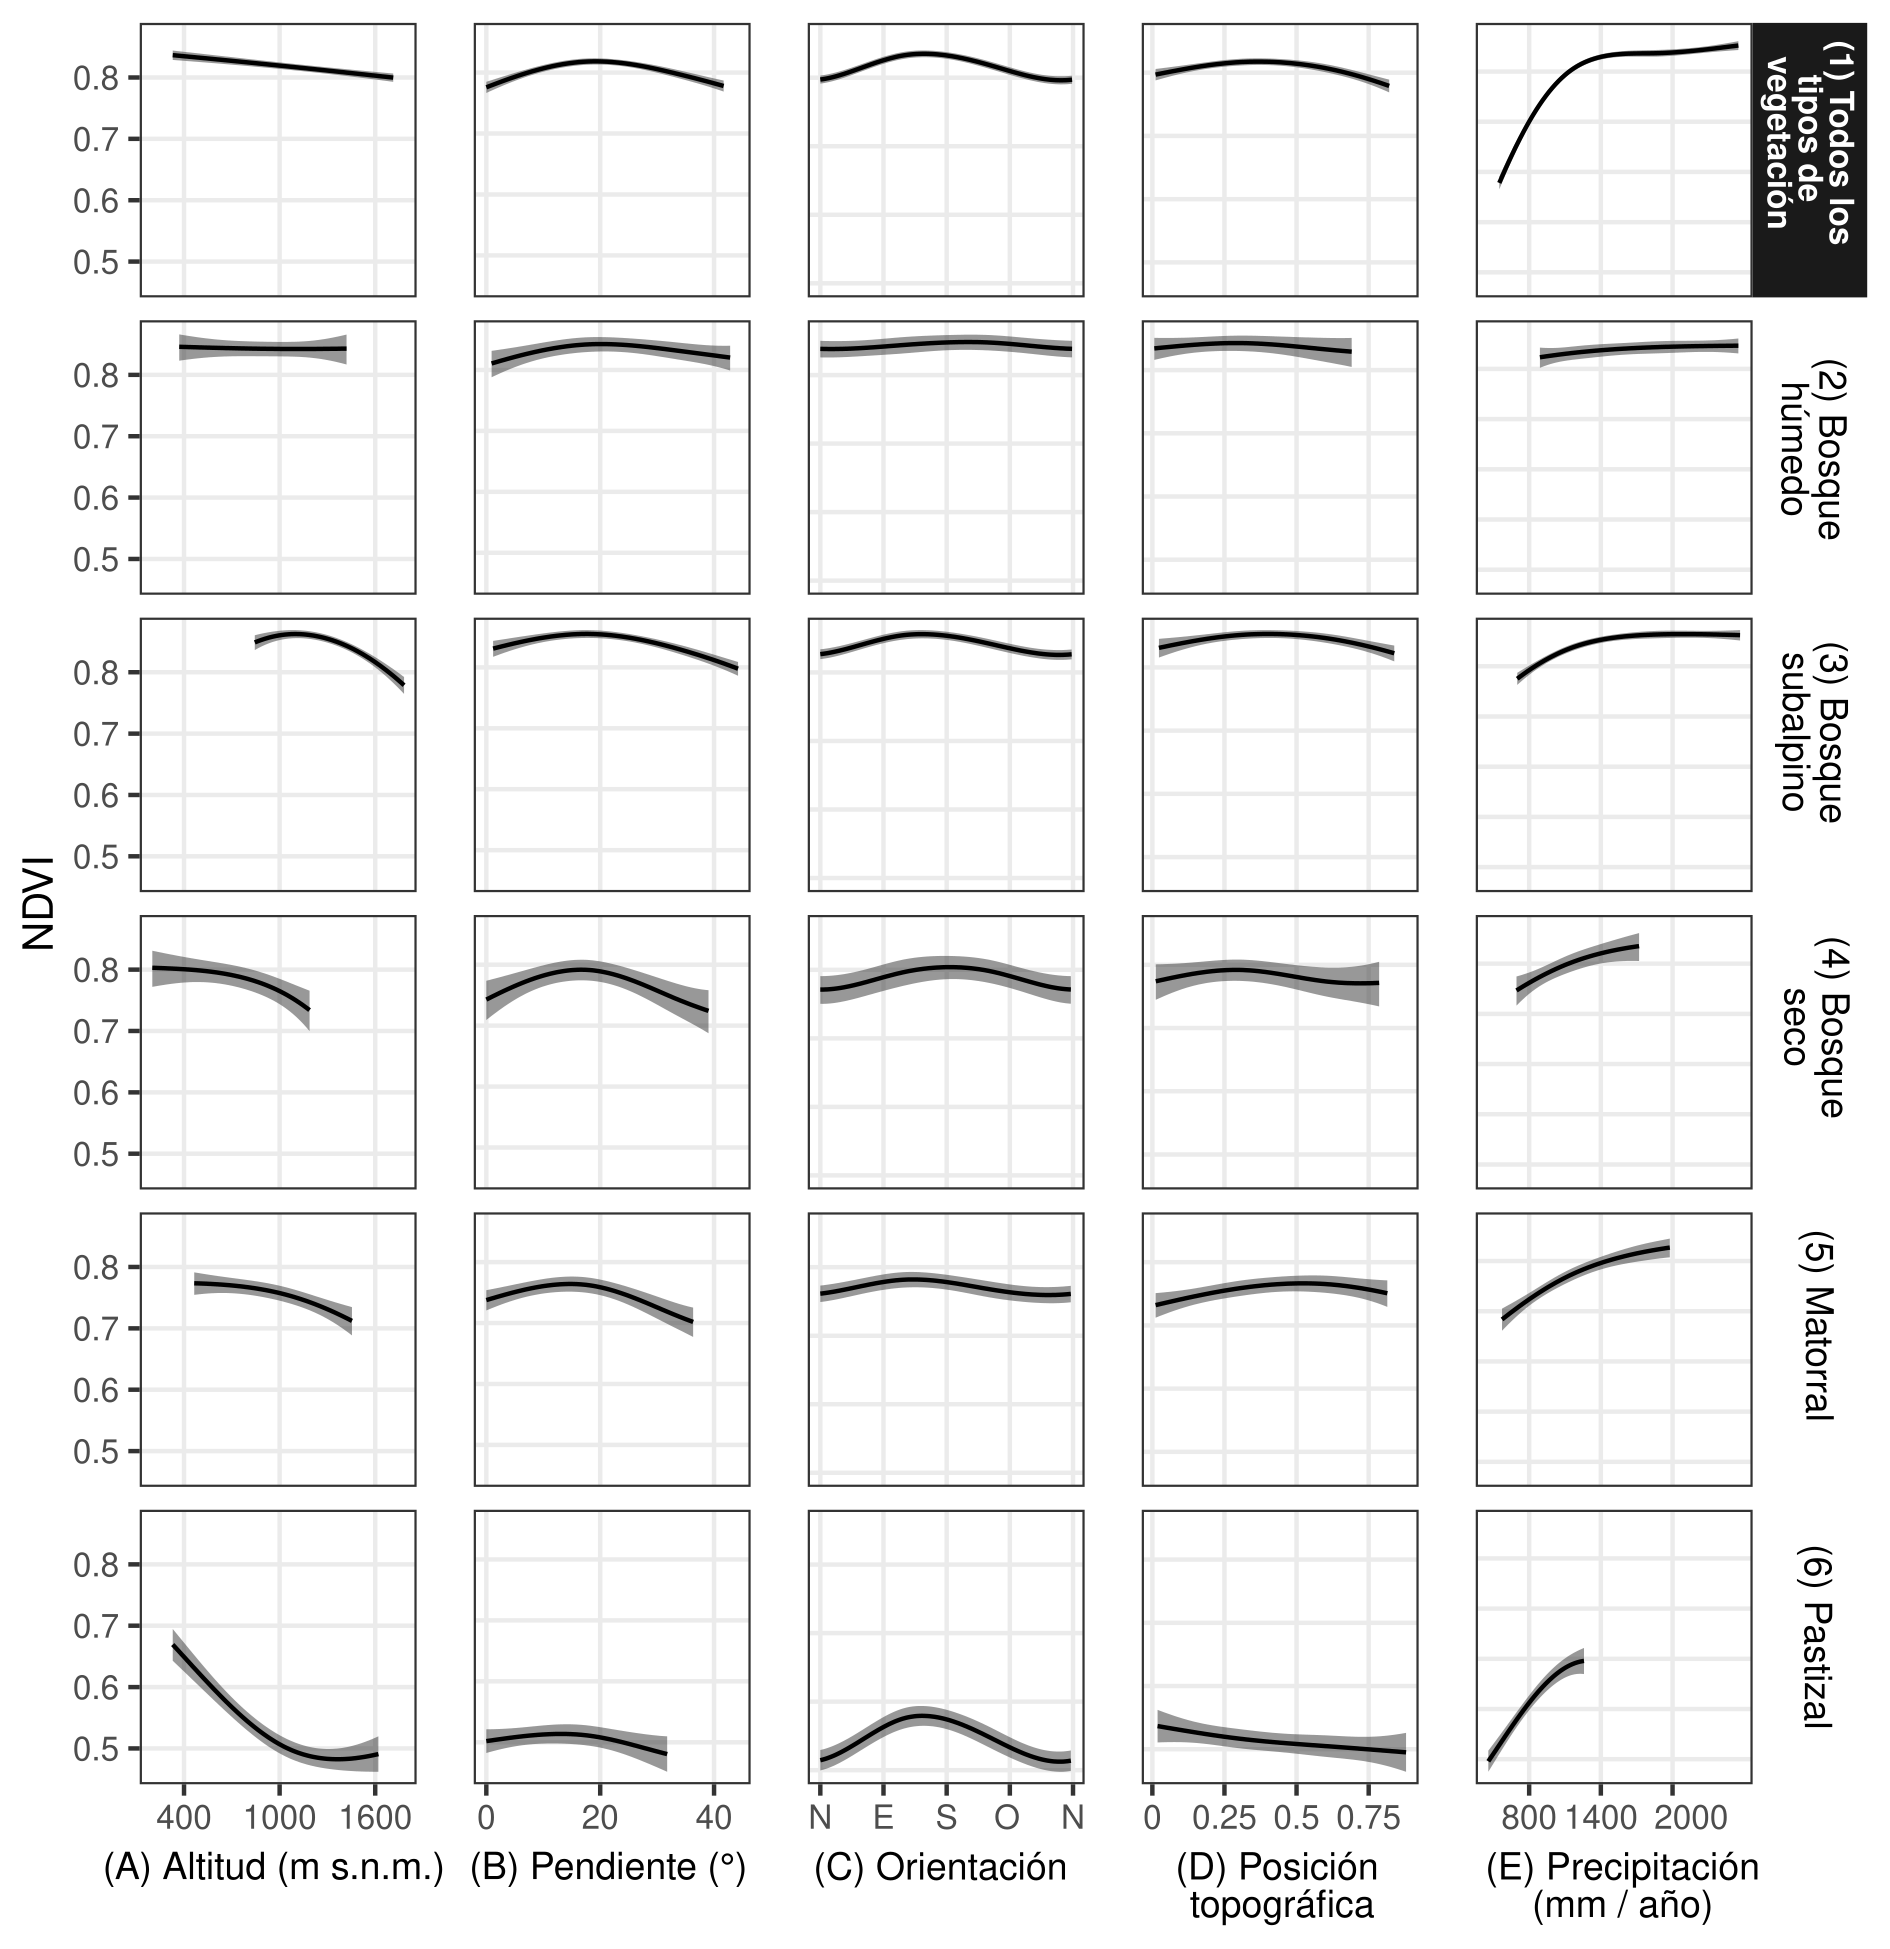
\includegraphics[width=16cm]{figuras/cap3/S07) ndvi_model_predictions.png}
    \caption[NDVI en función de variables ambientales.]{NDVI en función de variables topográficas y precipitación, calculado a lo largo del intervalo de máxima densidad del 98 \% en cada tipo de vegetación. Las líneas muestran la predicción a partir de la estimación de máxima verosimilitud, y las bandas, el intervalo de confianza del 95 \%.} 
    \label{fig:cap3-S07}
\end{figure}

\begin{figure}
    \centering
    \rotatebox[origin=c]{90}{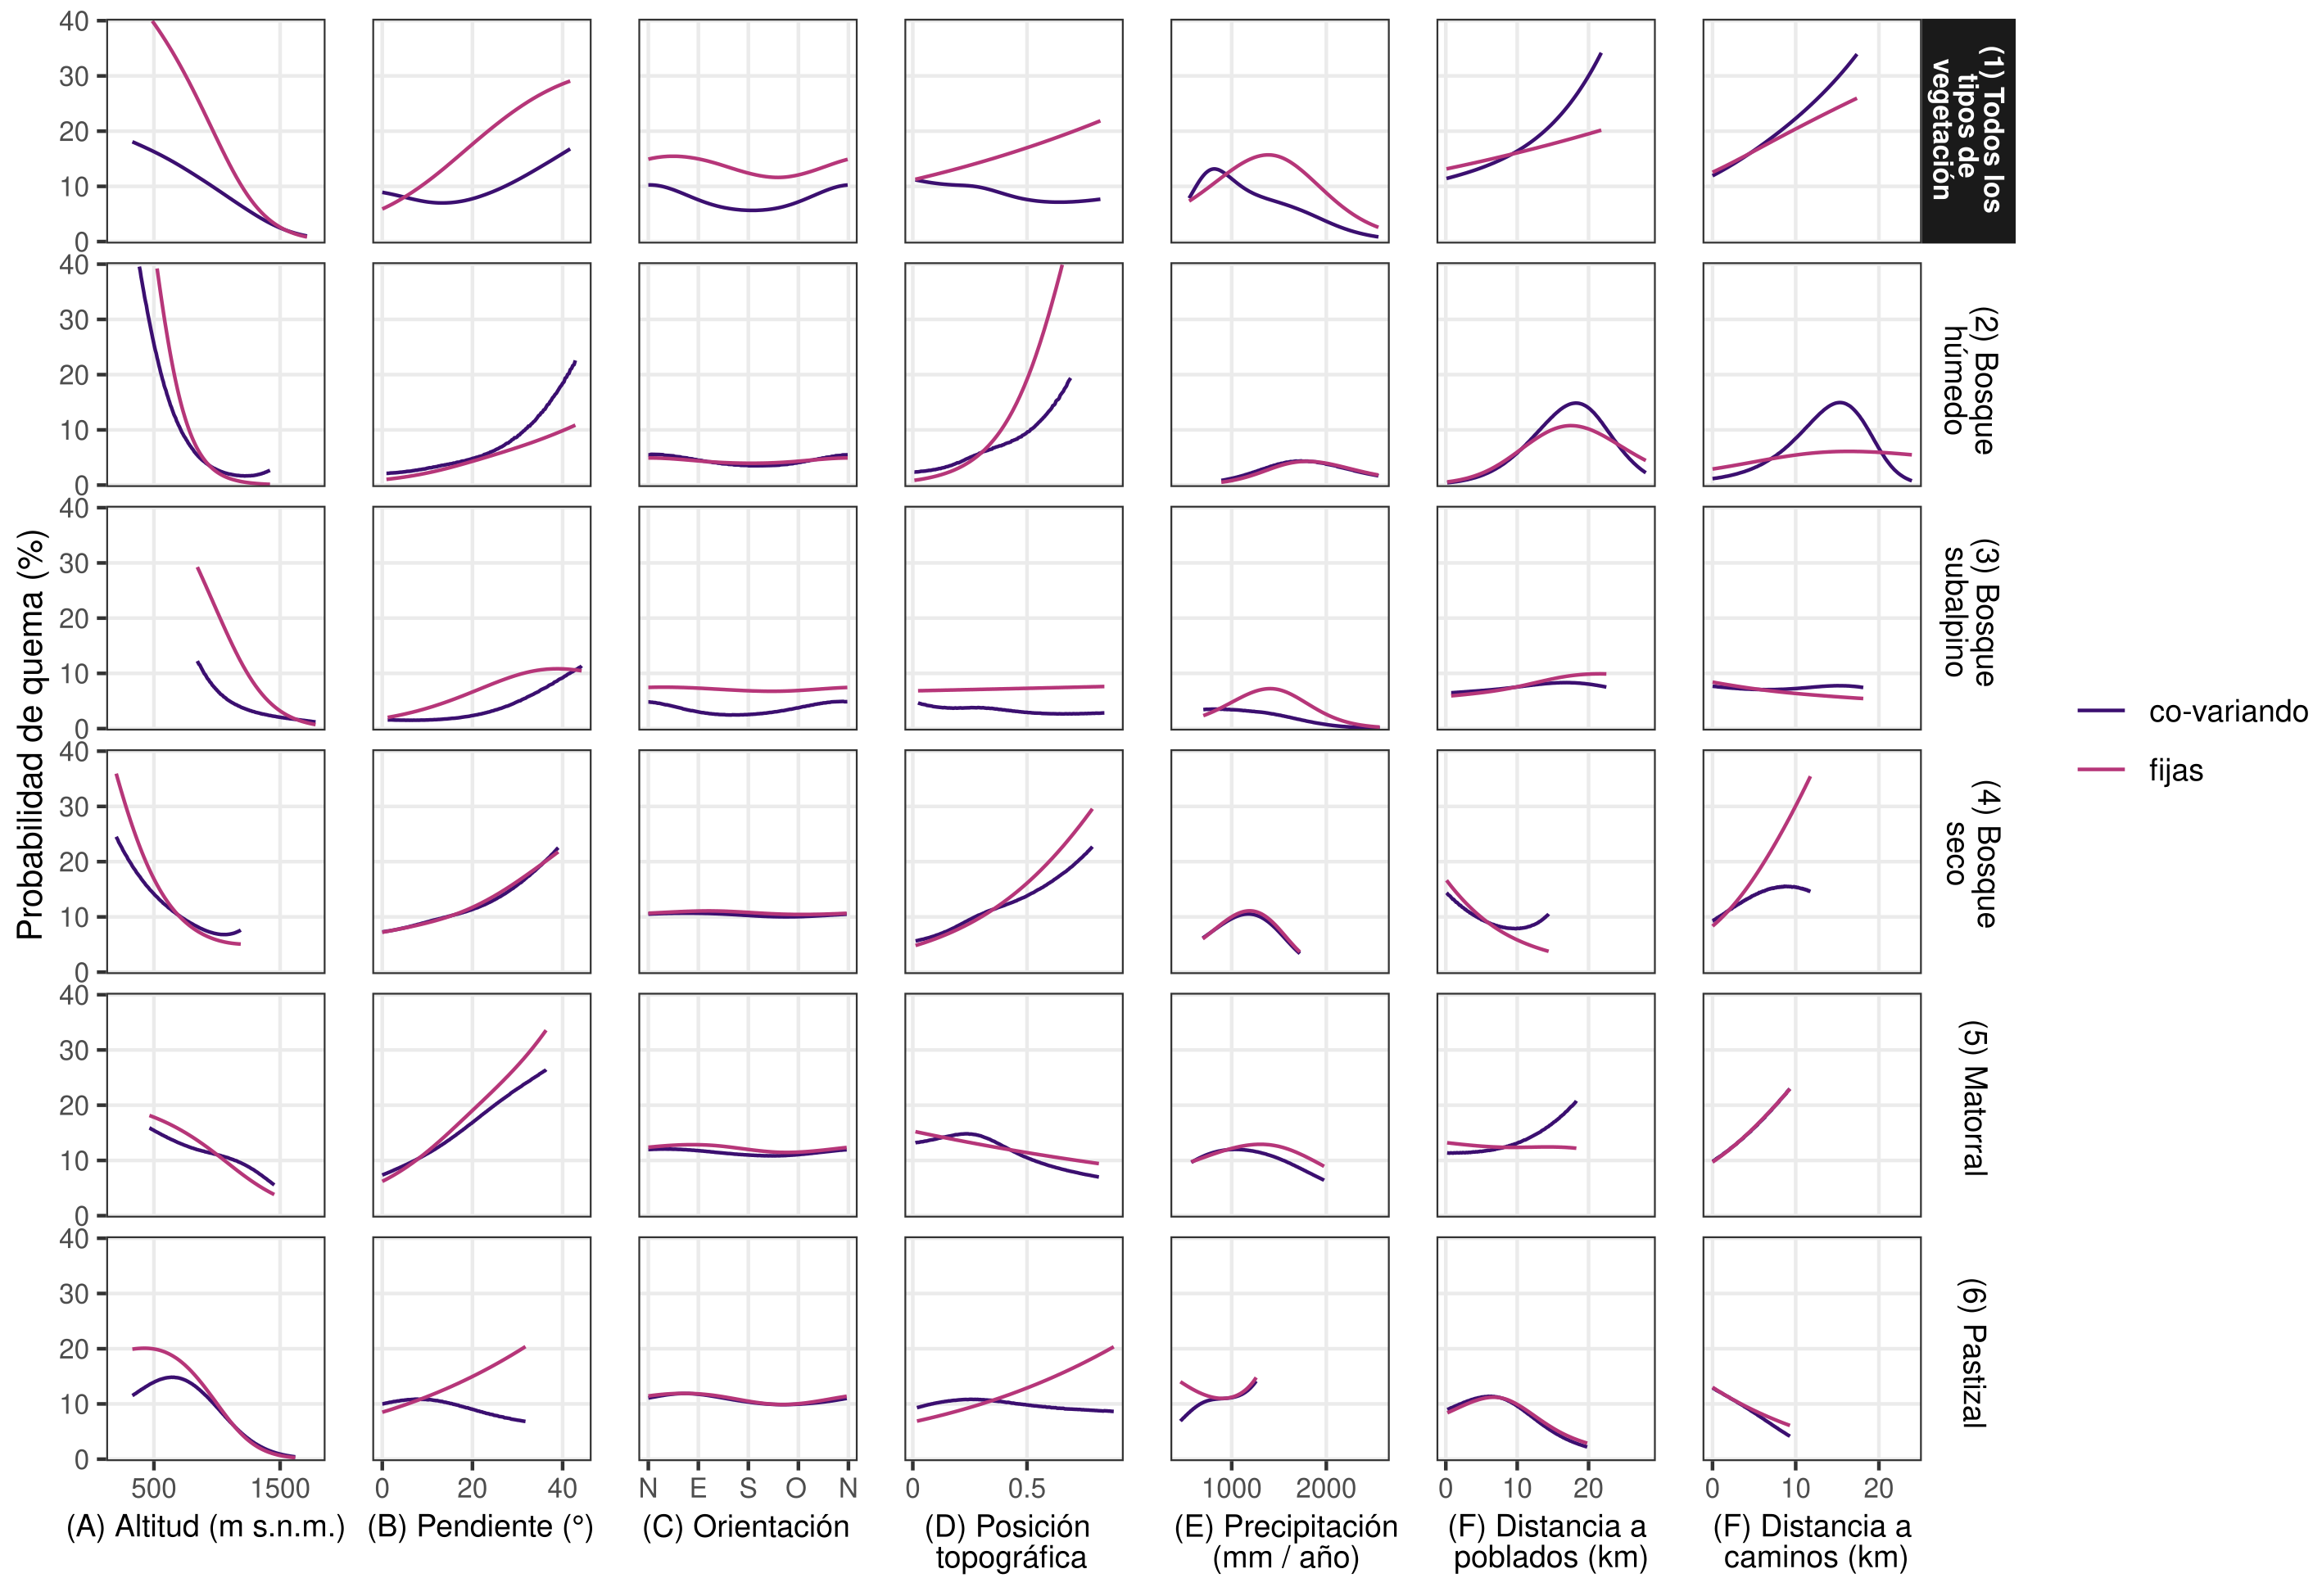
\includegraphics[width=0.95\textheight]{figuras/cap3/S08) burnprob_co-varying_fixed.png}}
    \caption[Probabilidad de quema covariando o fijando predictoras correlacionadas.]{(Leyenda en la página siguiente.)} 
    \label{fig:cap3-S08}
\end{figure}

% leyenda en la página siguiente
\begin{figure}[p]
  \contcaption{(en la página anterior). Probabilidad de quema en función de la topografía, la precipitación y la distancia a poblados y caminos, predicha considerando la covariación entre predictoras o no (predicciones fijas, estrictamente parciales). Las líneas más oscuras muestran las mismas predicciones que las Fig.~\ref{fig:cap3-04} y \ref{fig:cap3-05} del Capítulo~\ref{cap:patrones}.}
\end{figure}

\FloatBarrier

\subsection{Métrica de tamaño de efecto}\label{append:effsize}

Para las variables ambientales y el NDVI (predictoras continuas), el tamaño del efecto se definió como la desviación absoluta media de la curva de predicción no tan parcial, ponderando cada valor de la predictora por su densidad empírica, tanto para calcular la media a lo largo de la curva como para promediar la diferencia absoluta con respecto a la media. En el caso del tipo de vegetación, el cálculo fue similar, pero en lugar de utilizar una curva de predicción utilizamos la probabilidad de quema predicha para todos los tipos de vegetación, ya fuera a partir del modelo de vegetación, o a partir del PDP particionado calculado en base al modelo conjunto (sección~\ref{append:veg-comparison}). Para el modelo de vegetación, los pesos de cada tipo de vegetación se definieron como sus abundancias relativas en el paisaje. Cuando se compararon los tipos de vegetación en condiciones ambientales comunes con el modelo conjunto (PDP particionado), se calculó el tamaño del efecto del tipo de vegetación en cada partición. En ese caso, los pesos se definieron en base a la abundancia relativa de los tipos de vegetación comparados dentro de cada partición del conjunto de datos.

\subsection{Detección de patrones bajo correlación espacial}\label{append:pvalues}

Dado que la correlación espacial conduce a una subestimación de la incertidumbre, en lugar de calcular intervalos de confianza, evaluamos la incertidumbre comparando nuestros resultados con los de conjuntos de datos de incendios aleatorizados que presentaban una correlación similar. Simulamos 500 capas de ocurrencia de incendios, convirtiendo cada incendio observado en un círculo de la misma área y reubicando sus centroides al azar dentro del área quemable, permitiendo que los incendios se solaparan. Estas capas de incendios se rasterizaron y se muestrearon en los mismos 8228 puntos de los que se extrajeron los datos observados. A continuación, todos los análisis realizados con los datos observados se repitieron para cada de quema aleatorizada. Para los efectos de las predictoras continuas, calculamos los valores P a una cola como $1 - \pi$, donde $\pi$ es el percentil correspondiente al efecto observado en la distribución de efectos de los conjuntos de datos aleatorizados. Para las probabilidades de quema por tipo de vegetación, calculamos los valores P a dos colas de la siguiente manera: 

\begin{equation}
    \text{P} = 
    \begin{cases}
        \pi \ 2, & \text{para } \pi < 0.5 \\
        (1-\pi) \ 2 & \text{para } \pi \ge 0.5 
    \end{cases}
\label{eq:p-value}
\end{equation}

Donde $\pi$ es el percentil de la probabilidad de quema observada en la distribución de incendios aleatorios. Además, al graficar predicciones parciales para las predictoras continuas, calculamos los intervalos centrales de colas equiprobables (\textit{equal-tailed intervals}) del 80 \% y el 95 \% de todas las curvas de predicción parcial aleatorizadas (basadas en la estimación de máxima verosimilitud) y evaluamos visualmente en qué medida la curva obtenida con los datos observados se alejaba de esos intervalos.
\newpage{\ }
\cleardoublepage

\chapter{Apéndice Capítulo 4}\label{append_04}

\section{Índices de inflamabilidad}\label{append:FI}

Con el fin de parametrizar los índices de inflamabilidad, modelamos la probabilidad de que una celda se haya quemado al menos una vez en el período y área de estudio definidos en el Capítulo~\ref{cap:patrones} (1999-2022, 24 años). Extrajimos los datos de una muestra al azar de 9194 puntos tomados en la porción quemable del área de estudio, restringidos a tener una distancia mínima entre ellos de 800 m. El modelo fue definido de la siguiente manera:

\begin{equation}
\begin{aligned}
    y_i &\sim \ \text{Bernoulli}(\theta_i) \\
    \text{logit}(\theta_i) &= \alpha_{v[i]} + \beta_{v[i]} \ (NDVI_i - \omega_{v[i]}) \ +\gamma_1\ E_i + \gamma_2 \ N_i + \gamma_3 \ S_i \\
    \\
    \alpha_v &\sim \ \text{Normal}(\mu_{\alpha}, \sigma_{\alpha}) \\ 
    \log(-\beta_v) &\sim \ \text{Normal}(\mu_{\beta}, \sigma_{\beta}) \\
    \text{logit}(\omega_v) &\sim \ \text{Normal}(\mu_{\omega}, \sigma_{\omega}) \\
    \\
    \mu_{\alpha} &\sim \ \text{Normal}(0, 10) \\ 
    \sigma_{\alpha} &\sim \ \text{Normal}(0, 5)\text{T}[0, ] \\ 
    \\
    \mu_{\beta} &\sim \ \text{Normal}(\log(100), 2) \\ 
    \sigma_{\beta} &\sim \ \text{Normal}(0, 2)\text{T}[0, ] \\ 
    \\
    \mu_{\omega} &\sim \ \text{Normal}(0, 5) \\ 
    \sigma_{\omega} &\sim \ \text{Normal}(0, 3)\text{T}[0, ] \\ 
    \\
    \gamma_k &\sim \ \text{Normal}(0, 10),\ \text{con } k \in \{1, 2, 3\}.
\end{aligned}
\end{equation}

\noindent $y_i \in \{0, 1\}$ indica si la celda $i$ se quemó o no en el período de estudio, $\theta_i$ es su probabilidad de quema, $E$ es la altitud, $N$ es el componente norte de la orientación ponderado por la pendiente (orientación norte, ver~\eqref{eq:FI}), y $S$ es la pendiente de la ladera. Las tres variables topográficas fueron estandarizadas para el ajuste, pero luego sus parámetros fueron transformados a la escala original de las variables. El subíndice $v[i]$ indica el tipo de vegetación $\in \{1, ..., 5\}$ correspondiente a la celda $i$, y numerados de acuerdo a la Tabla~\ref{tab:fi_params_veg}. Los parámetros asociados a los efectos de la vegetación ($\alpha$, $\beta$, y $\omega$) fueron estimados con previas jerárquicas para facilitar la estimación de los tipos de vegetación con pocos datos, como el bosque seco. Nótese que se forzó a que $\beta$ fuera negativo para que el efecto del NDVI fuera unimodal. El efecto de la pendiente ($\gamma_3$) no era de interés para calcular el índice de inflamabilidad por topografía (IIT), pero se incluyó para mejorar la estimación de los demás parámetros. El efecto de la pendiente se toma en cuenta de forma separada en el modelo de propagación, pero en ese caso, es un efecto direccional, ya que varía según la propagación ocurra cuesta arriba o cuesta abajo. En \eqref{eq:FI} los índices son escalados para que tengan media 0 y desvío 1 en el conjunto de datos usado para ajustar este modelo.

\begin{figure}[htbp]
  \centering 
  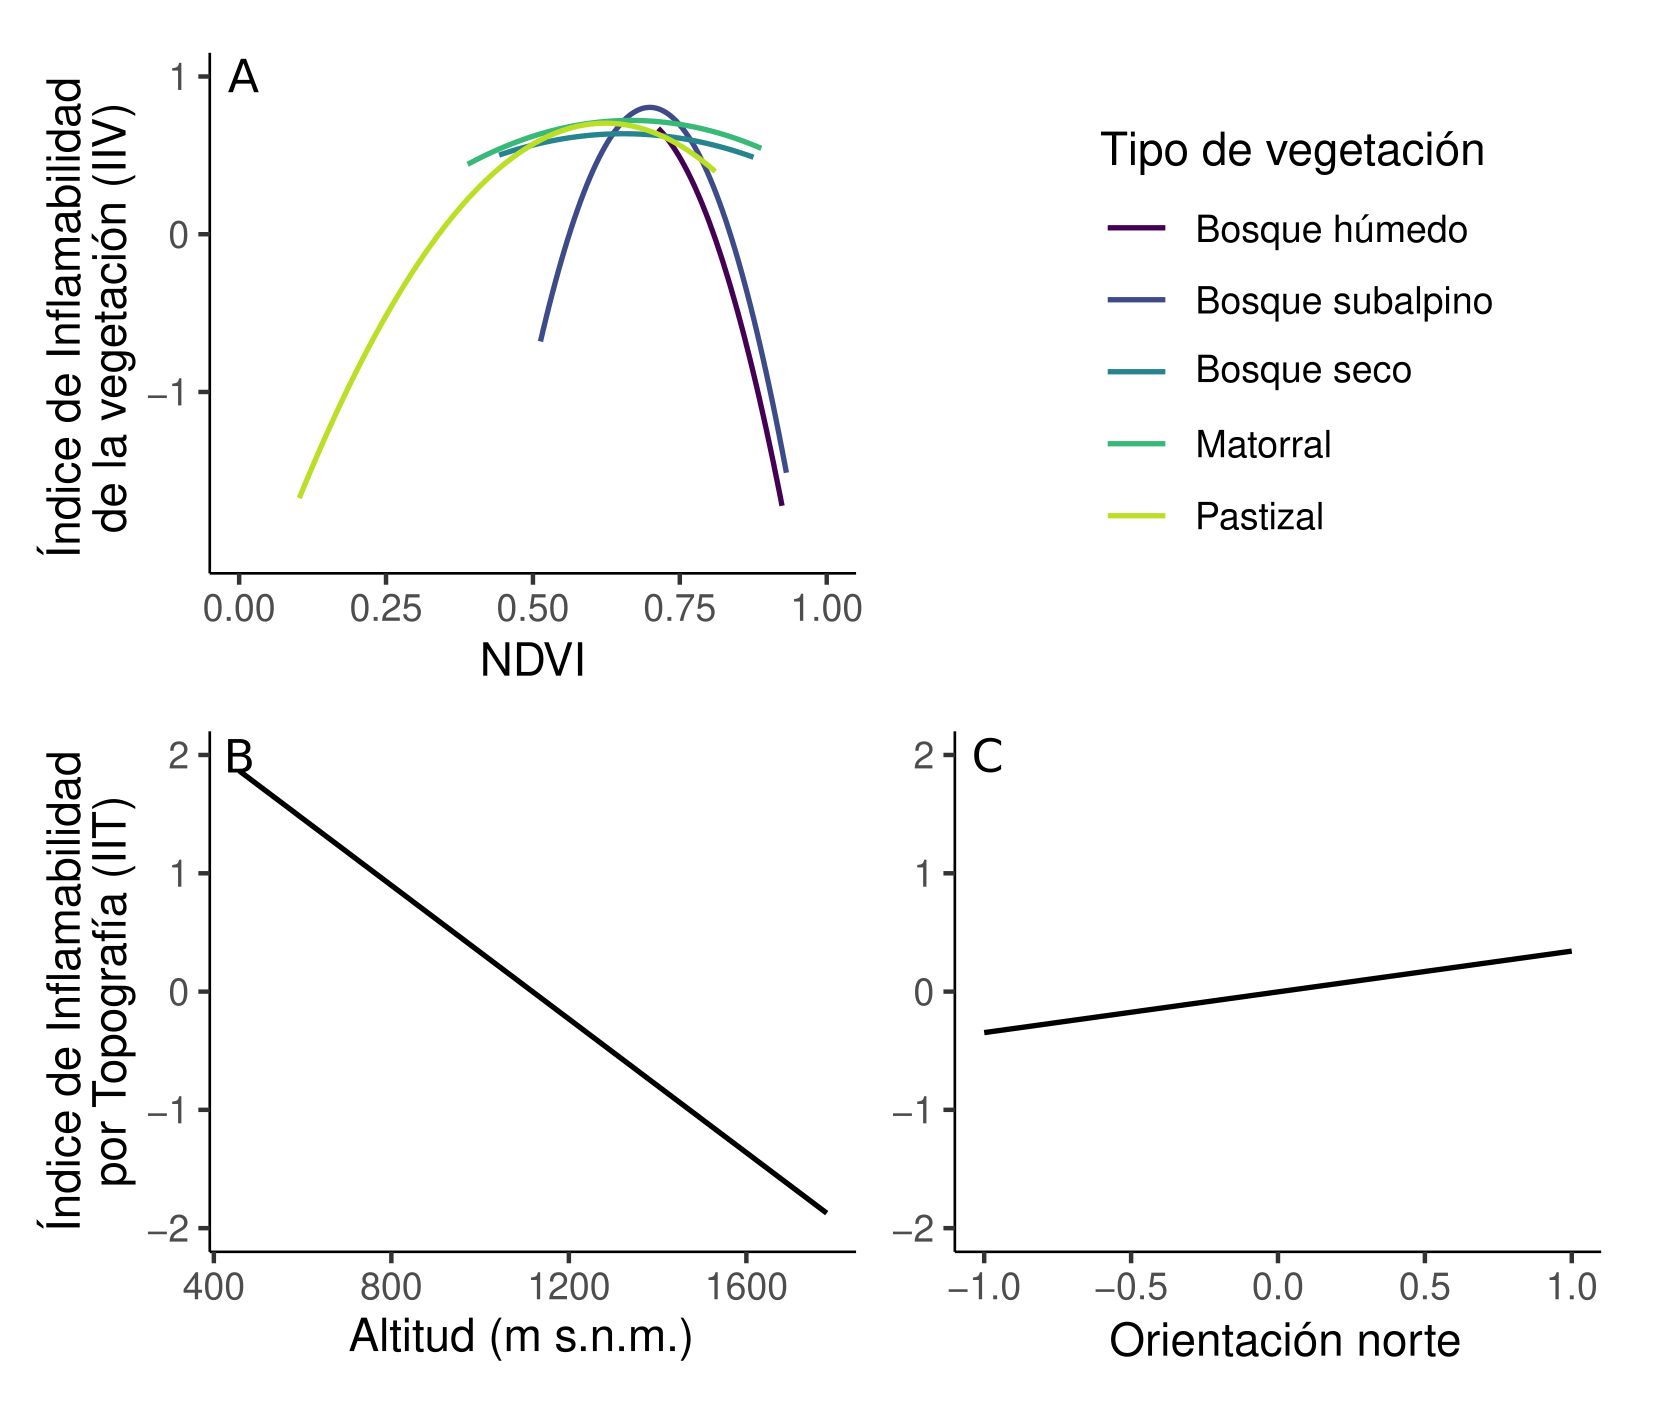
\includegraphics[width=14cm]{figuras/cap4/spread/flammability_indices.png}
  \caption{Índices de inflamabilidad en función de las variables que los componen, definidos en \eqref{eq:FI}.}
  \label{fig:FI}
\end{figure}

\FloatBarrier

\section{Proyecciones del régimen de incendios bajo cambio climático}\label{append:proj}

Los valores de FWI diario en su escala original diferían considerablemente entre las simulaciones de los modelos climáticos \citep{quilcaille2023FWI} y los datos basados en el reanálisis de ERA5 \citep{vitolo_era5-based_2020}, pero las anomalías quincenales de FWI presentaban una distribución muy similar. Sin embargo, dado que los datos y las simulaciones diferían en escala, las anomalías diarias de las simulaciones fueron calculadas a partir de la media y el desvío estándar del FWI basado también en simulaciones. Para cada realización de cada modelo climático y en cada escenario, las anomalías diarias de FWI fueron calculadas para los 3 períodos (1999-2023, 2040-2049, 2090-2099) de la siguiente manera:

\begin{enumerate}
    \item Definir período de referencia como la concatenación de la simulación climática para el final del escenario histórico (1999-2015) y el comienzo del escenario futuro correspondiente (2016-2023). 
    \item Calcular la media y desvío estándar de los valores diarios por celda en ese período.
    \item Estandarizar los valores diarios por celda en base a la media y desvío definidos en (2). Esto se hace para todos los días en los 3 períodos de interés: moderno, 2040s y 2090s.
    \item Promediar las anomalías diarias por quincena. 
\end{enumerate}

De esta manera, los valores se estandarizaron en base a la misma serie simulada. El período moderno de las simulaciones fue utilizado únicamente para evaluar cómo los modelos representaban el clima en dicho período, con el fin de ponderar los modelos adecuadamente. Para cada serie simulada de anomalías quincenales de FWI del período moderno (1999-2023) evaluamos su similitud con los datos basados en ERA5 mediante el índice de Bhattacharyya $B \in [0, 1]$, definido como:

\[
B(f, g) = \int \sqrt{f(x) \ g(x)}\ dx,
\]

\noindent donde $f()$ y $g()$ son las funciones de densidad de probabilidad. En este caso, estas densidades se obtuvieron por estimación basada en kernel utilizando los datos de ERA5 y las simulaciones. Previamente, remuestreamos los rasters a la resolución de ERA5 y recortamos todos al contorno del PNNH. Como cada modelo climático tenía un set de datos para el período moderno por cada escenario climático y realización, promediamos $B$ entre escenarios y realizaciones para obtener un único valor por modelo. En base a esta métrica definimos el peso de cada modelo como $P = \exp\{-[(1 - B) / 6]^2\}$ (no normalizado), para ponderar su aparición en las simulaciones de acuerdo a su capacidad de reproducir el clima observado. La Tabla~\ref{tab:climtable} detalla los modelos y realizaciones utilizados.

\begin{table}[htbp]
\centering
\caption[Modelos climáticos utilizados para las proyecciones.]{Modelos climáticos utilizados para las proyecciones. $B \in [0, 1]$ es el índice de similitud de Bhattacharyya entre las distribuciones de anomalía de FWI quincenal según el reanálisis de ERA5 o de las simulaciones climáticas. Los pesos se muestran relativizados al máximo para facilitar la comparación.}
\label{tab:climtable}
\small
\begin{tabular}{L{3cm} C{1.5cm} C{1.5cm} L{8cm}}
\toprule
Modelo & $B$ & Peso ($P$) & Realizaciones \\
\midrule
ACCESS-CM2 & 0.992 & 0.999 & r2i1p1f1, r3i1p1f1, r4i1p1f1, r5i1p1f1\\
ACCESS-ESM1-5 & 0.962 & 0.951 & r10i1p1f1, r11i1p1f1, r12i1p1f1, r13i1p1f1, r14i1p1f1, r15i1p1f1, r16i1p1f1, r17i1p1f1, r18i1p1f1, r19i1p1f1, r1i1p1f1, r20i1p1f1, r21i1p1f1, r22i1p1f1, r23i1p1f1, r24i1p1f1, r25i1p1f1, r26i1p1f1, r27i1p1f1, r28i1p1f1, r29i1p1f1, r2i1p1f1, r30i1p1f1, r31i1p1f1, r32i1p1f1, r33i1p1f1, r34i1p1f1, r35i1p1f1, r36i1p1f1, r37i1p1f1, r38i1p1f1, r39i1p1f1, r3i1p1f1, r40i1p1f1, r4i1p1f1, r5i1p1f1, r6i1p1f1, r7i1p1f1, r8i1p1f1, r9i1p1f1\\
CanESM5 & 0.979 & 0.986 & r10i1p1f1, r10i1p2f1, r11i1p1f1, r11i1p2f1, r12i1p1f1, r12i1p2f1, r13i1p1f1, r13i1p2f1, r14i1p1f1, r14i1p2f1, r15i1p1f1, r15i1p2f1, r16i1p1f1, r16i1p2f1, r17i1p1f1, r17i1p2f1, r18i1p1f1, r18i1p2f1, r19i1p1f1, r19i1p2f1, r1i1p1f1, r20i1p1f1, r20i1p2f1, r21i1p1f1, r21i1p2f1, r22i1p1f1, r22i1p2f1, r23i1p1f1, r23i1p2f1, r24i1p1f1, r24i1p2f1, r25i1p1f1, r25i1p2f1, r2i1p1f1, r2i1p2f1, r3i1p1f1, r3i1p2f1, r4i1p1f1, r4i1p2f1, r5i1p1f1, r5i1p2f1, r6i1p1f1, r6i1p2f1, r7i1p1f1, r7i1p2f1, r8i1p1f1, r8i1p2f1, r9i1p1f1, r9i1p2f1\\
CMCC-ESM2 & 0.980 & 0.987 & r1i1p1f1\\
EC-Earth3 & 0.984 & 0.993 & r1i1p1f1, r4i1p1f1\\
FGOALS-g3 & 0.989 & 0.997 & r1i1p1f1, r3i1p1f1\\
INM-CM4-8 & 0.978 & 0.984 & r1i1p1f1\\
INM-CM5-0 & 0.993 & 1.000 & r1i1p1f1\\
IPSL-CM6A-LR & 0.993 & 1.000 & r14i1p1f1, r1i1p1f1, r2i1p1f1, r3i1p1f1, r4i1p1f1, r6i1p1f1\\
MIROC-ES2L & 0.976 & 0.981 & r10i1p1f2, r1i1p1f2, r2i1p1f2, r4i1p1f2, r5i1p1f2, r6i1p1f2, r7i1p1f2, r8i1p1f2, r9i1p1f2\\
MIROC6 & 0.990 & 0.998 & r1i1p1f1, r2i1p1f1, r3i1p1f1\\
MPI-ESM1-2-HR & 0.947 & 0.905 & r1i1p1f1, r2i1p1f1\\
MPI-ESM1-2-LR & 0.951 & 0.919 & r10i1p1f1, r11i1p1f1, r12i1p1f1, r13i1p1f1, r14i1p1f1, r15i1p1f1, r16i1p1f1, r17i1p1f1, r18i1p1f1, r19i1p1f1, r1i1p1f1, r20i1p1f1, r21i1p1f1, r22i1p1f1, r23i1p1f1, r24i1p1f1, r25i1p1f1, r26i1p1f1, r27i1p1f1, r28i1p1f1, r29i1p1f1, r2i1p1f1, r30i1p1f1, r3i1p1f1, r4i1p1f1, r5i1p1f1, r6i1p1f1, r7i1p1f1, r8i1p1f1, r9i1p1f1\\
MRI-ESM2-0 & 0.831 & 0.358 & r1i1p1f1, r2i1p1f1, r3i1p1f1, r4i1p1f1, r5i1p1f1\\
\bottomrule
\end{tabular}
\end{table}

\FloatBarrier

\section{Efecto de la vegetación sobre la probabilidad de propagación en función del FWI}\label{append:spread-veg-effects}

Un aspecto relevante del modelo de propagación era cómo cambiaba el efecto del tipo de vegetación sobre la probabilidad de propagación con el FWI. Si bien el coeficiente asociado a la vegetación ($\beta_1$, IIV; Ecuación~\ref{eq:datamodel}) no varió en función del FWI (Fig.~\ref{fig:spread-params}B), la no linealidad de la función logística hace que el efecto de una variable sobre la probabilidad de propagación dependa también del efecto y del valor de otras variables, incluso cuando no hay coeficientes de interacción, como en nuestro modelo. Esto es relevante porque el FWI afectó a otros coeficientes de propagación, como aquellos regulando el efecto del viento y la pendiente ($\beta_3$ y $\beta_4$; Ecuación~\ref{eq:datamodel}; Fig.~\ref{fig:spread-params}Dy E). Si al aumentar el FWI el efecto del viento aumentaba lo suficiente como para llevar la probabilidad de propagación cerca de 1 (Fig.~\ref{fig:spread-curves}D), el efecto de la vegetación podría atenuarse, al menos considerando propagación a favor del viento. Para evaluar la posibilidad de esta interacción implícita, evaluamos cómo cambiaba el efecto del tipo de vegetación sobre la probabilidad de propagación en función del FWI, considerando los efectos del FWI sobre todos los parámetros de propagación. 

Para poder comparar los tipos de vegetación, fijamos la altitud en 900 m s.n.m. y la orientación en 90~° (implicando orientación norte = 0), fijando así el IIT (Índice de Inflamabilidad por Topografía). Para considerar en la predicción el efecto direccional de la pendiente y el viento sobre la probabilidad de propagación, considerando su variabilidad en el PNNH, muestreando 500 celdas de su zona quemable, utilizando el raster creado para la simulación de incendios, que contenía, entre otras variables, la velocidad del viento y la pendiente (Sección~\ref{cap4:data}). Para considerar el efecto de la pendiente tanto cuesta arriba como cuesta abajo, duplicamos el conjunto de celdas y fijando la pendiente en 0° en la segunda mitad (el modelo de propagación asume que la propagación cuesta abajo es igual que en llano; Ecuación~\ref{eq:datamodel}). 

Para comparar los tipos de vegetación necesitábamos obtener el IIV (Índice de Inflamabilidad de la Vegetación) para cada uno, con lo cual, requeríamos el NDVI. Como el NDVI varía en función de la topografía, calculamos su valor esperado para las condiciones topográficas analizadas (500 valores de pendiente, con altitud y orientación fijas) utilizando un modelo de NDVI, con un enfoque similar a lo expuesto en el Apéndice~\ref{append:cov}. Ajustamos un Modelo Aditivo Generalizado con distribución Beta para el NDVI  escalado a [0, 1], utilizando el mismo conjunto de datos con el cual se estimaron los parámetros de los índices de inflamabilidad (Apéndice~\ref{append:FI}). Incluimos como predictoras la pendiente, altitud y orientación en base a resultados del Capítulo~\ref{cap:patrones} (Fig.~\ref{fig:cap3-S07}). Con este modelo predijimos el NDVI a 900 m de altitud, con orientación este, y sobre todos los valores de pendiente muestreados, con el cual, calculamos el IIV para cada tipo de vegetación en todas las celdas muestreadas.

En base a la altitud y orientación fijadas, a los 500 valores de pendiente y viento muestreados (además de los 500 valores con pendiente fijada en cero), con sus respectivos IIV para cada tipo de vegetación, calculamos la probabilidad de propagación por tipo de vegetación a lo largo de una secuencia de FWI, promediando las predicciones a lo largo de las celdas muestreadas. De esta manera, las predicciones condicionan en valores fijos de altitud, orientación y tipo de vegetación y marginalizan sobre la distribución de velocidad del viento, pendiente y NDVI en el PNNH, asumiendo siempre dirección del viento a favor de la propagación. Además, las predicciones se calcularon marginalizando sobre los efectos aleatorios mediante simulación. 

El efecto del tipo de vegetación sobre la probabilidad de propagación (Fig.~\ref{fig:spread-veg-effects}A) se definió como el desvío absoluto medio a lo largo de los cinco tipos de vegetación, ponderándolos a todos por igual. 

\section{Propagación, resultados extendidos}\label{append:spread_results}

\begin{figure}[H]
  \centering 
  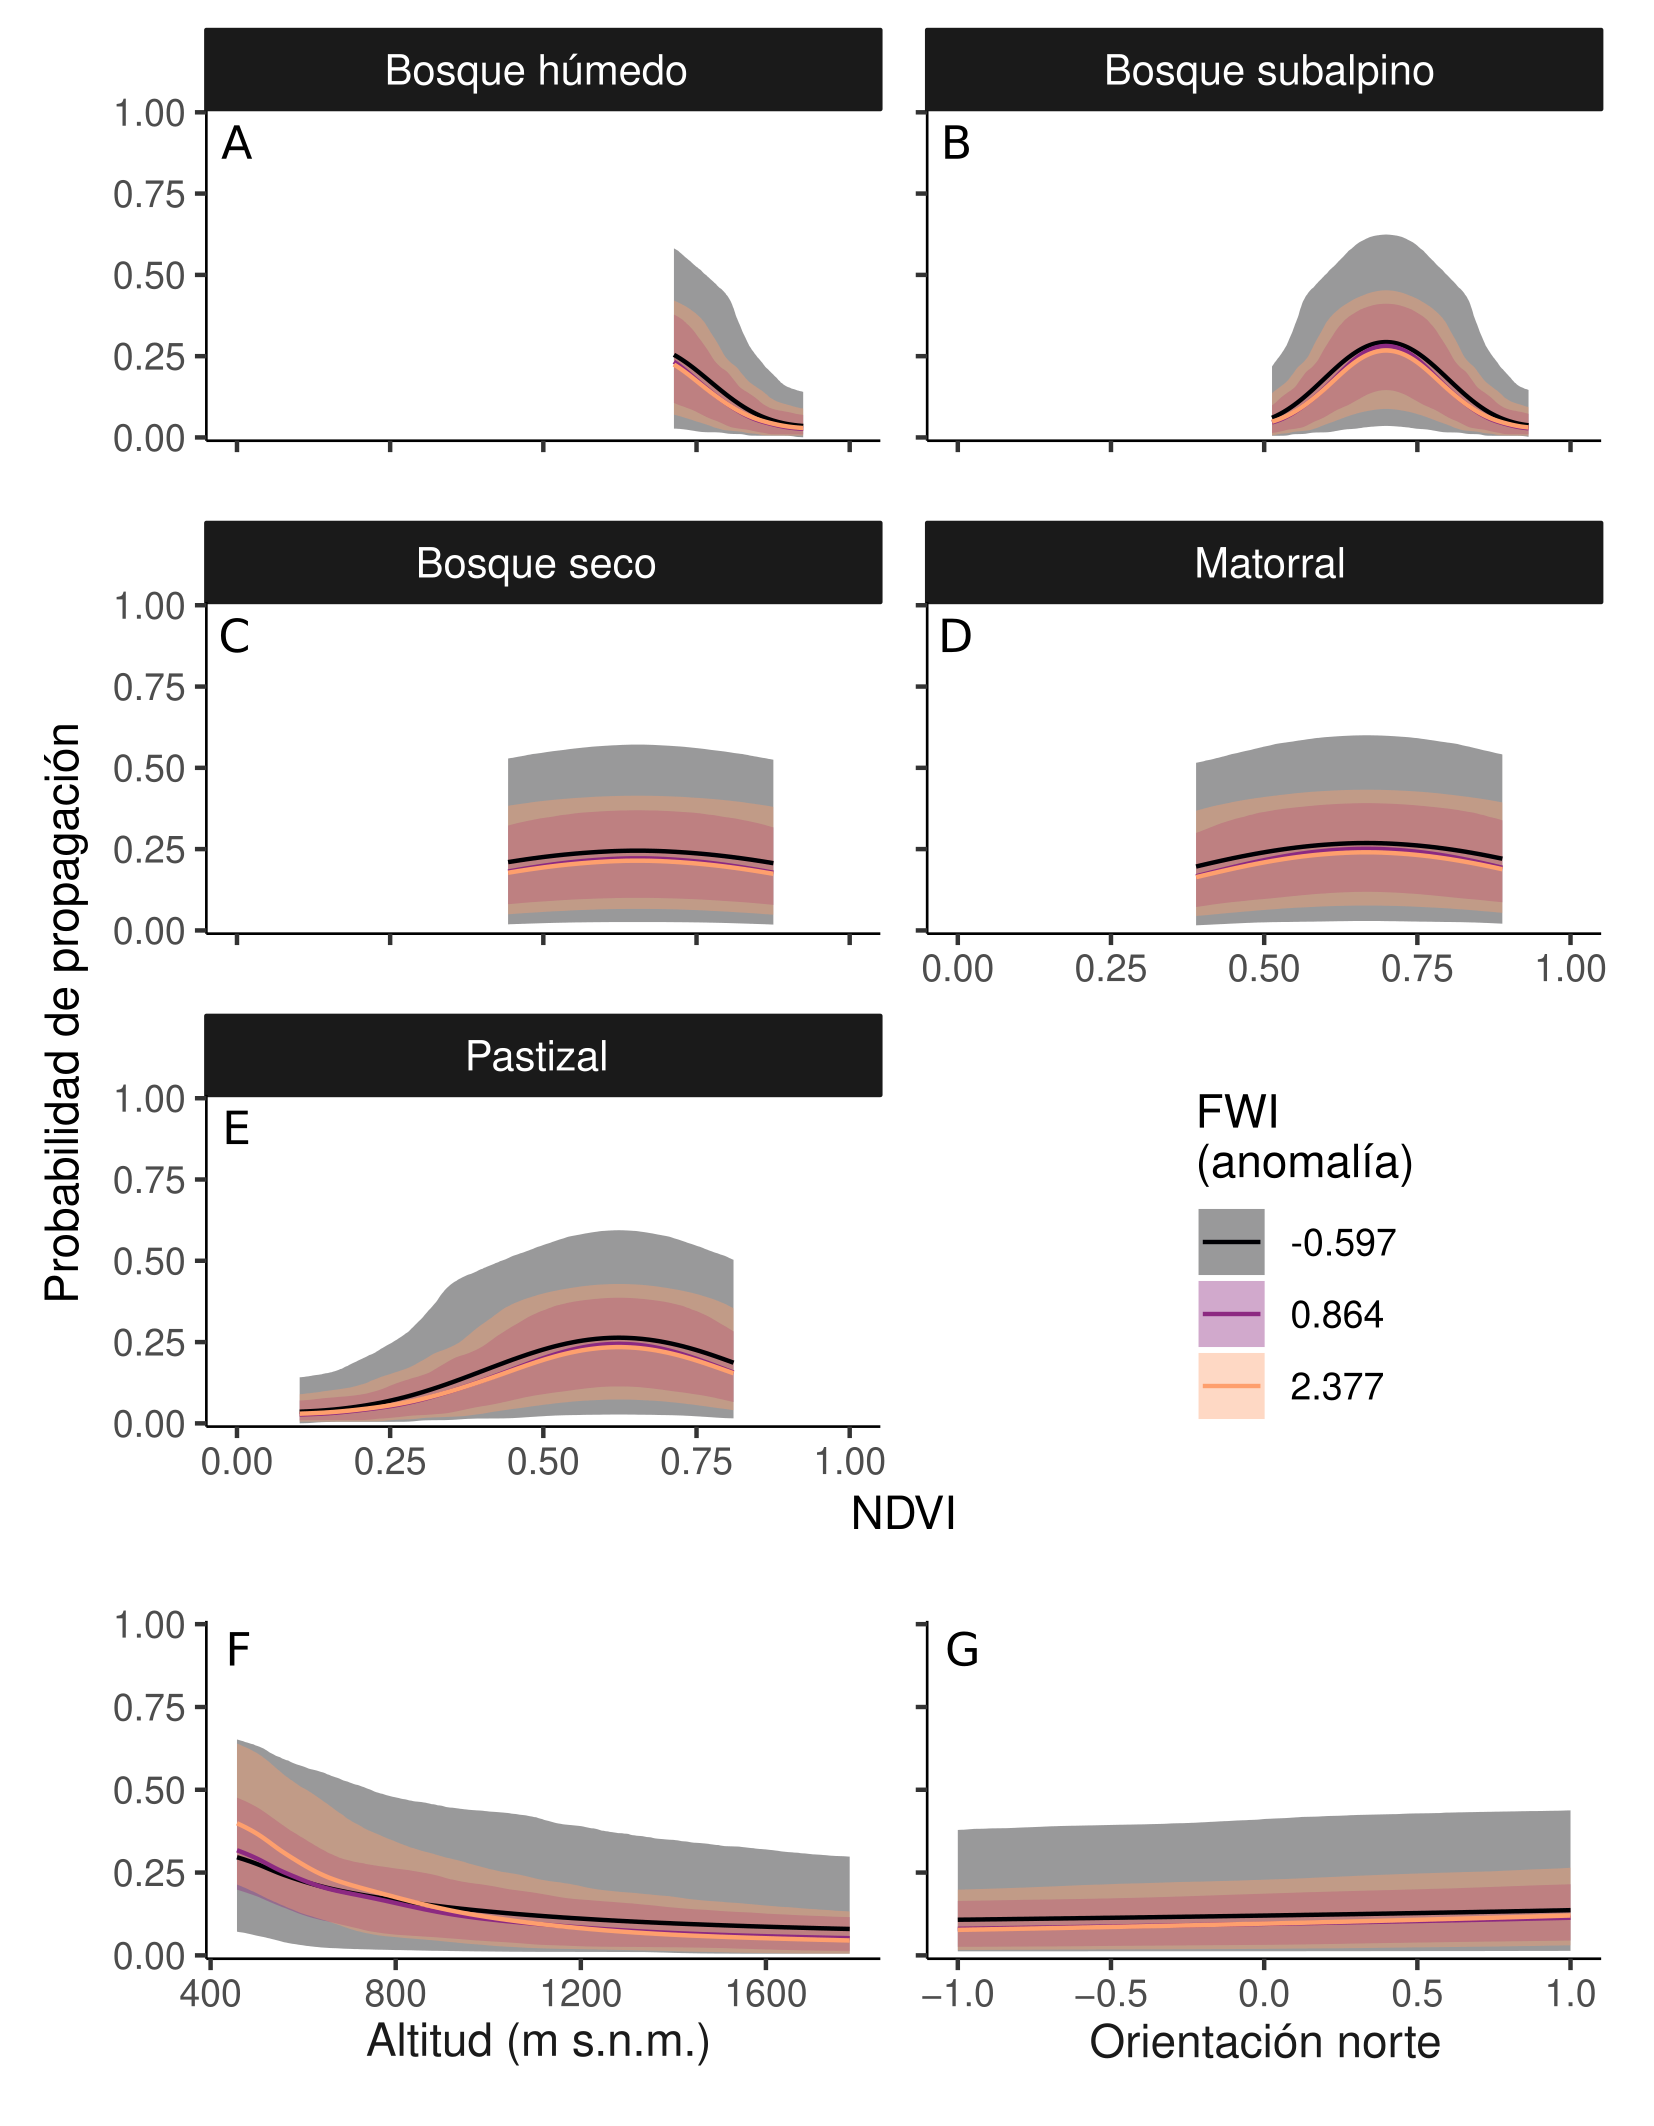
\includegraphics[width=14cm]{figuras/cap4/spread/spread_prob_curves_raw_x.png}
  \caption[Probabilidad de propagación en función del NDVI, el tipo de vegetación, la altitud y la orientación.]{Probabilidad de propagación en función las predictoras, descomponiendo los índices de inflamabilidad de vegetación y por topografía en sus variables crudas.}
  \label{fig:spread-curves-x}
\end{figure}

\begin{figure}[htbp]
  \centering 
  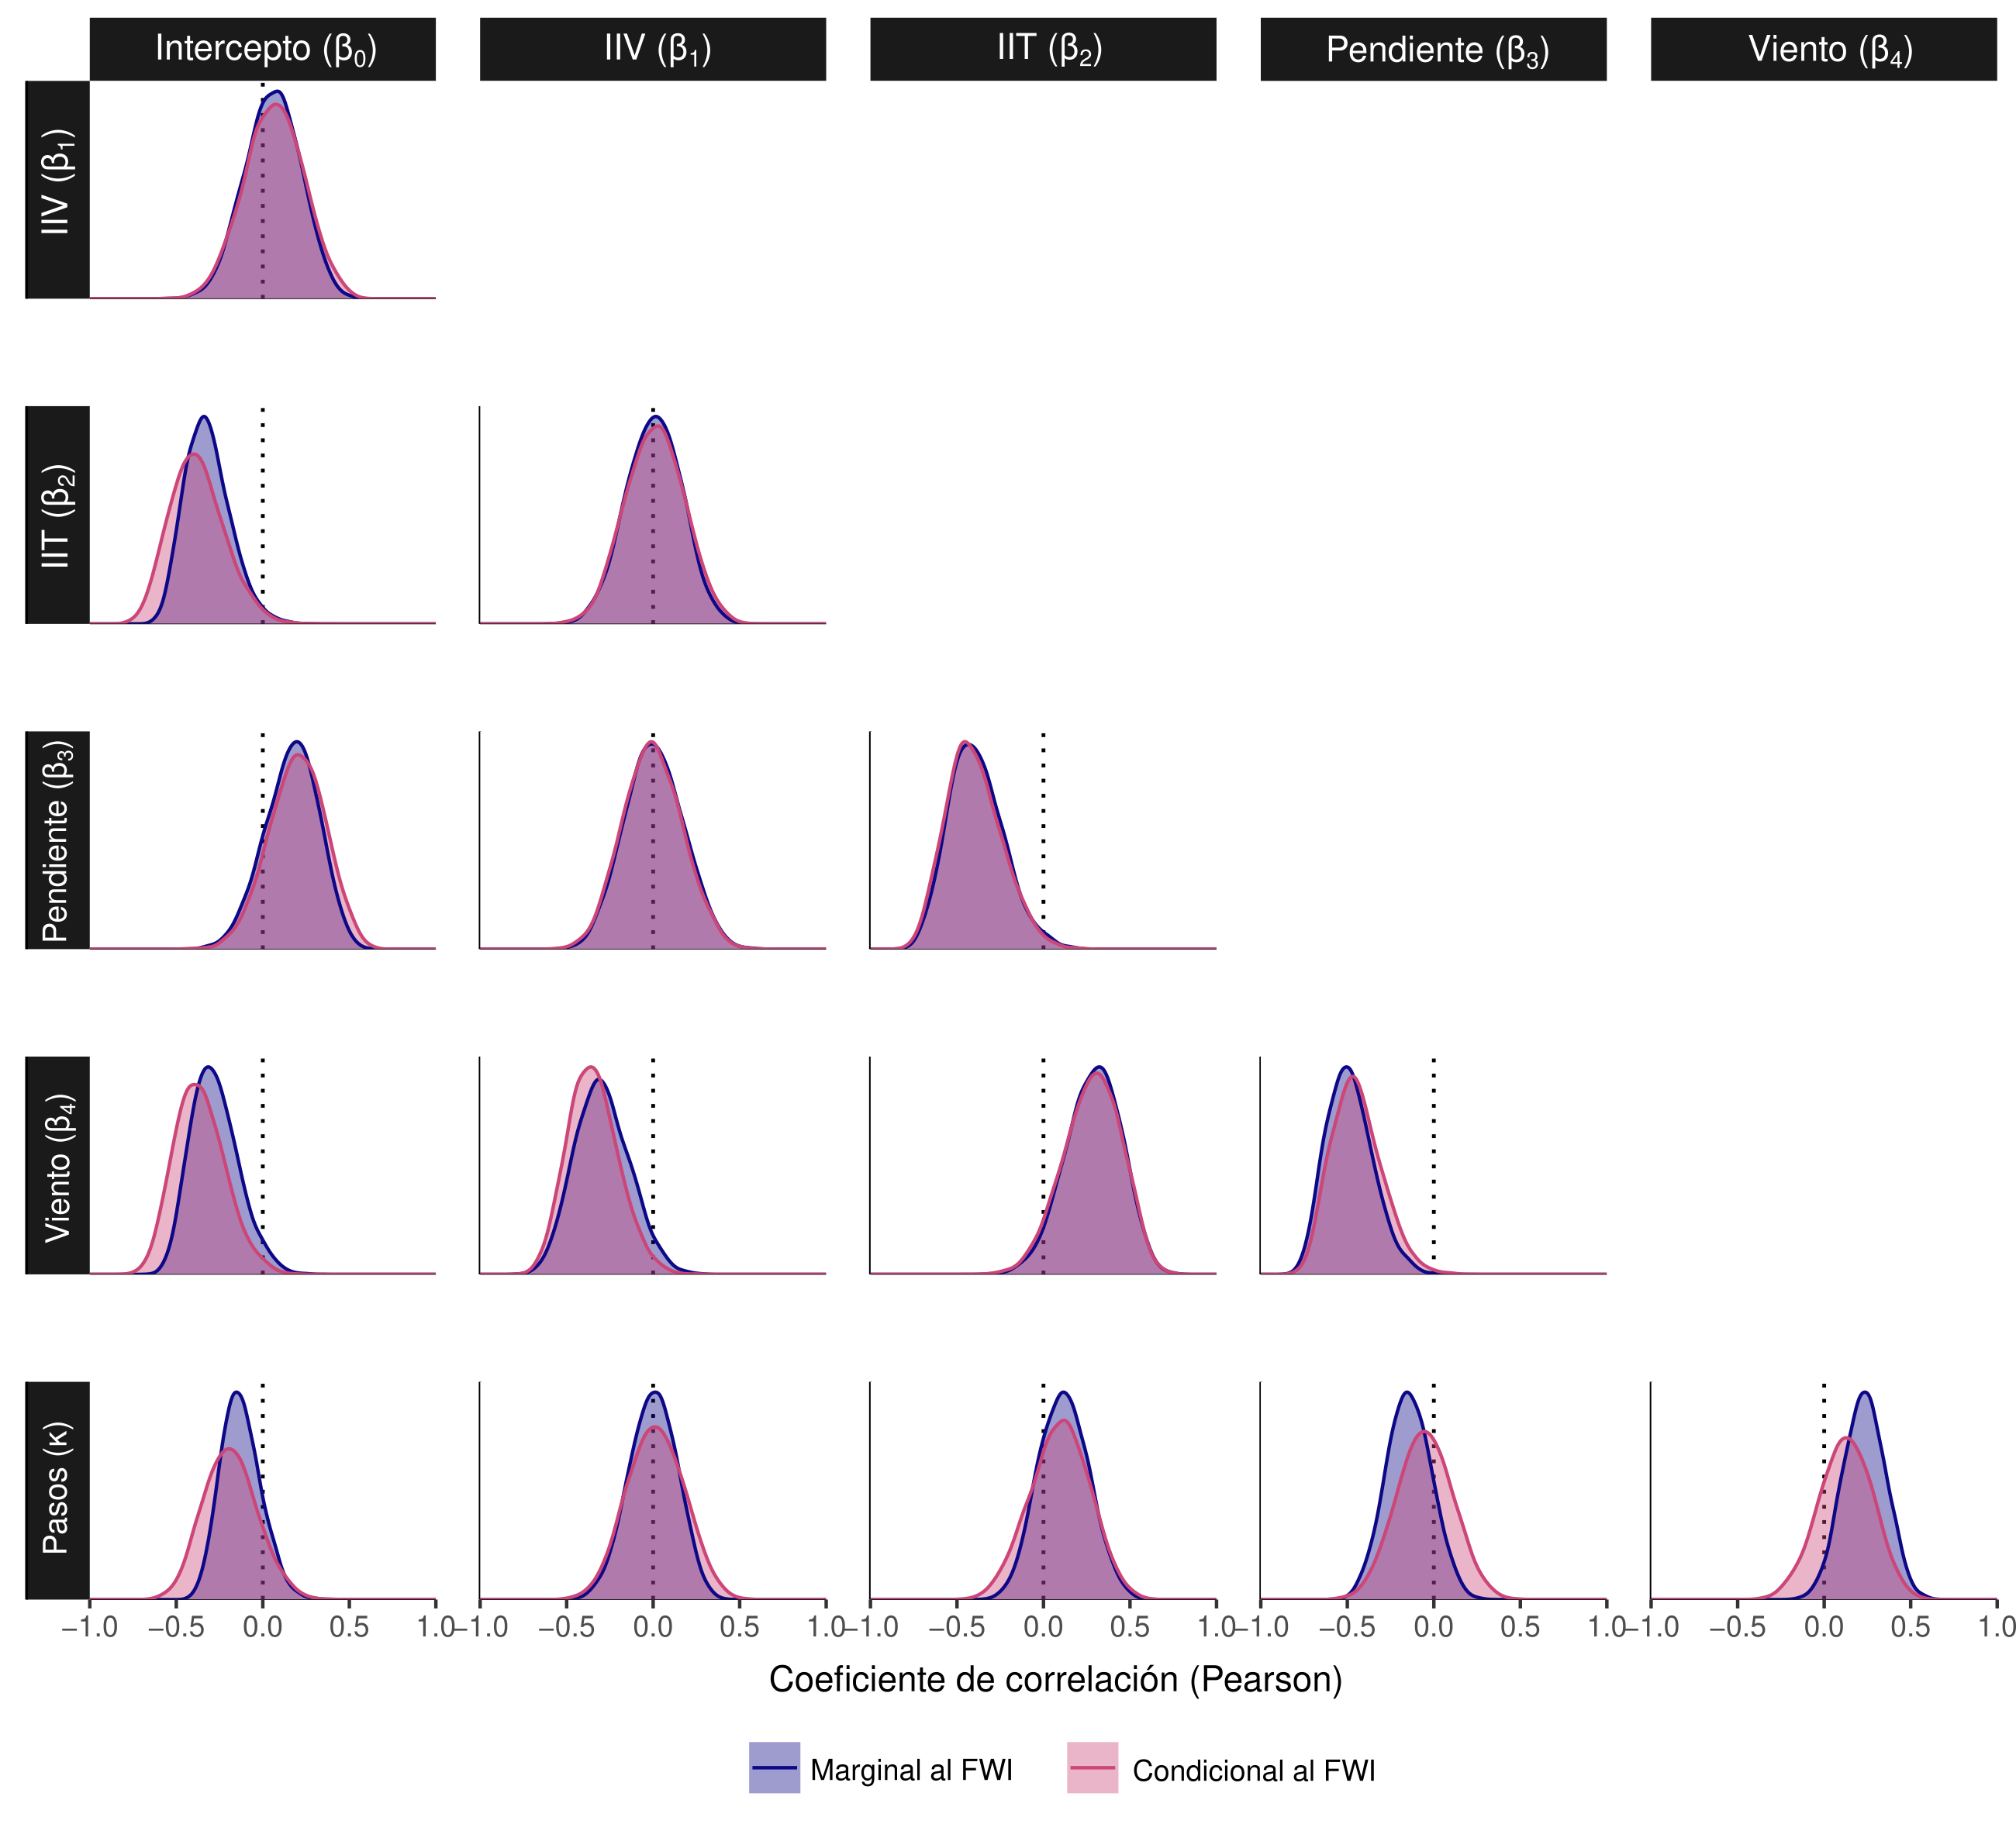
\includegraphics[width=\textwidth]{figuras/cap4/spread/pairs_plot_correlations_posteriors.png}
  \caption[Correlación entre los parámetros de propagación.]{Distribución posterior del coeficiente de correlación de Pearson entre cada par de parámetros de propagación, condicional o incondicional al FWI. Los coeficientes fueron calculados simulando valores de la Normal Multivariada ajustada. Las distribuciones condicionales al FWI fijan el FWI en la media de los datos de propagación, y representan la posterior de $\boldsymbol{\Omega}$ (ver Ecuación~\ref{eq:hier2}). La distribución incondicional al FWI incluye su efecto FWI: parámetros que son afectados de forma similar (diferente) por el FWI presentaría una correlación incondicional de mayor (menor) magnitud que la condicional.}
  \label{fig:spread-corr}
\end{figure}

\FloatBarrier

Las siguientes figuras muestran el ajuste del modelo de propagación. Como describimos en la sección~\ref{cap4:spread-model}, para cada incendio se estimó un vector de parámetros $\boldsymbol{\beta}$, el cual regula la propagación. Permitir que estos parámetros variaran entre incendios fue una forma de representar variables no observadas relevantes para el fuego. Por ejemplo, un incendio que fue apagado rápidamente por combatientes o por lluvia puede presentar un menor número de pasos ($\kappa$) que el promedio, y un incendio que propagó con elevada velocidad del viento puede presentar un efecto fuerte del viento ($\beta_4$). A su vez, a partir la variabilidad en $\boldsymbol{\beta}$ entre incendios y de cómo esta variabilidad se relacionaba con el FWI de cada incendio, estimamos una distribución de parámetros (Ecuación~\ref{eq:hier1}), que nos permite simular nuevos $\boldsymbol{\beta}$ para incendios hipotéticos. Para evaluar el ajuste del modelo comparar incendios observados con incendios simulados. Pero existen dos formas de hacerlo: (1) utilizar los \textit{parámetros ajustados} para cada incendio, o (2) simular nuevos parámetros de la distribución estimada (\textit{parámetros simulados}). Es esperable que en el primer caso los incendios simulados se parezcan más a los observados, en cambio, utilizando parámetros simulados estamos simulando incendios que difieren de los observados en las variables no observadas representadas por estos parámetros (e.g., velocidad del viento, combate, precipitaciones, etc.).

\begin{figure}[htbp]
  \centering 
  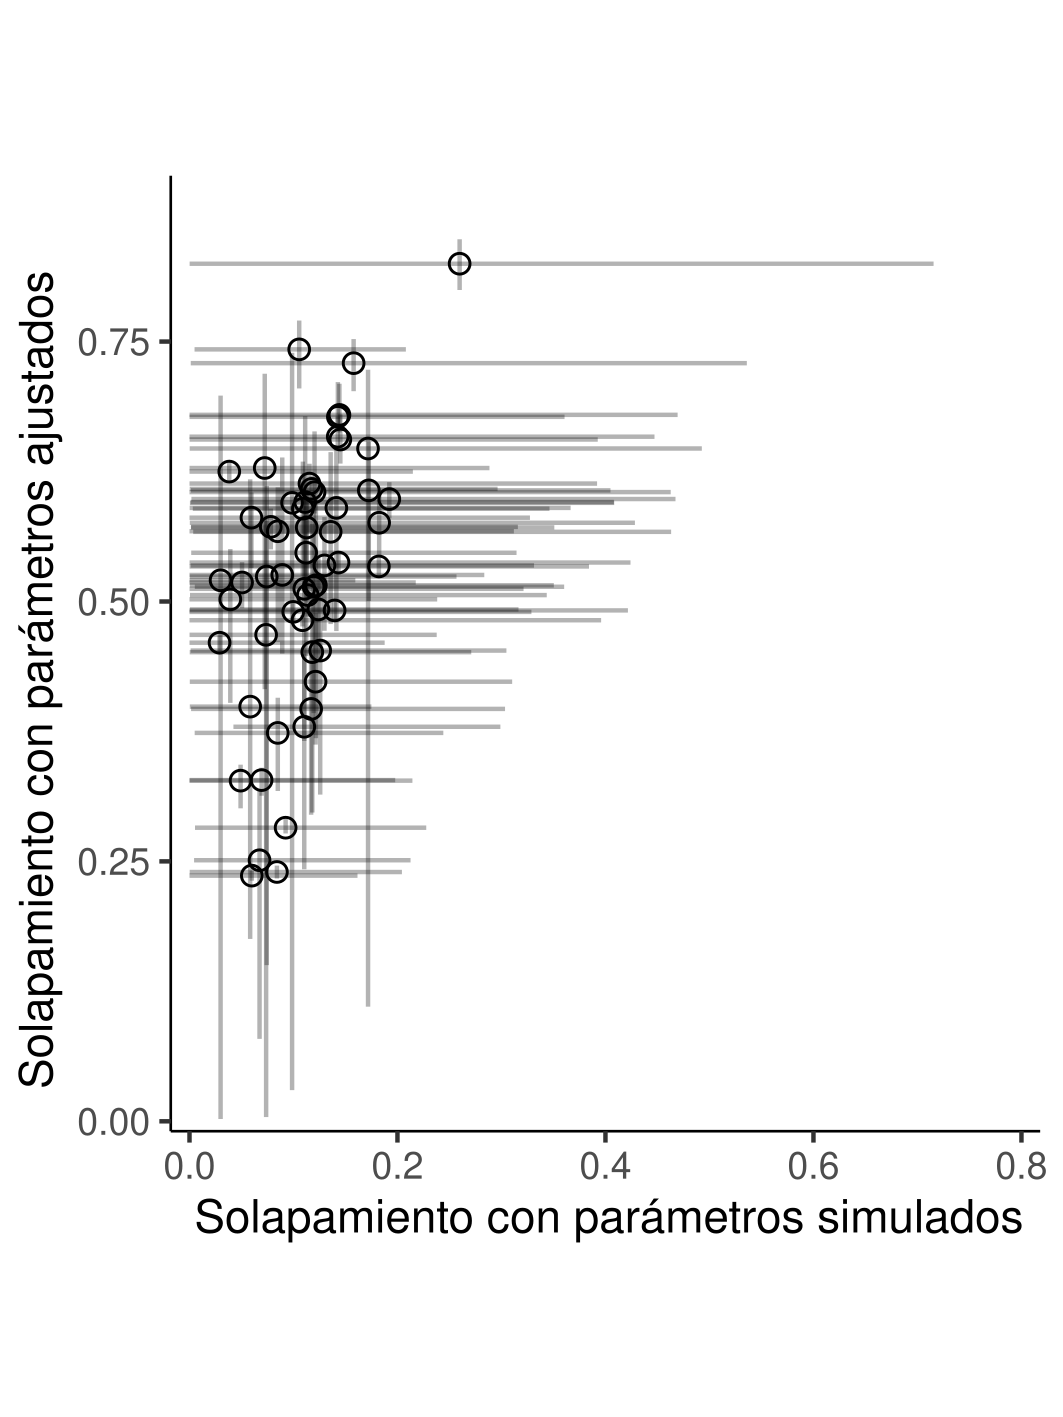
\includegraphics[width=9cm]{figuras/cap4/spread/overlap_fit_sim.png}
  \caption[Solapamiento espacial entre incendios simulados y observados.]{Solapamiento espacial entre incendios simulados y observados, utilizando los parámetros ajustados para cada incendio o simulando nuevos parámetros a partir de la distribución estimada. Los puntos y líneas indican la media y el intervalo de credibilidad del 95 \% de la distribución posterior del solapamiento, aproximada mediante 2000 simulaciones para cada tipo de uso de los parámetros e incendio.}
  \label{fig:spread-ov}
\end{figure}

\begin{figure}[htbp]
  \centering 
  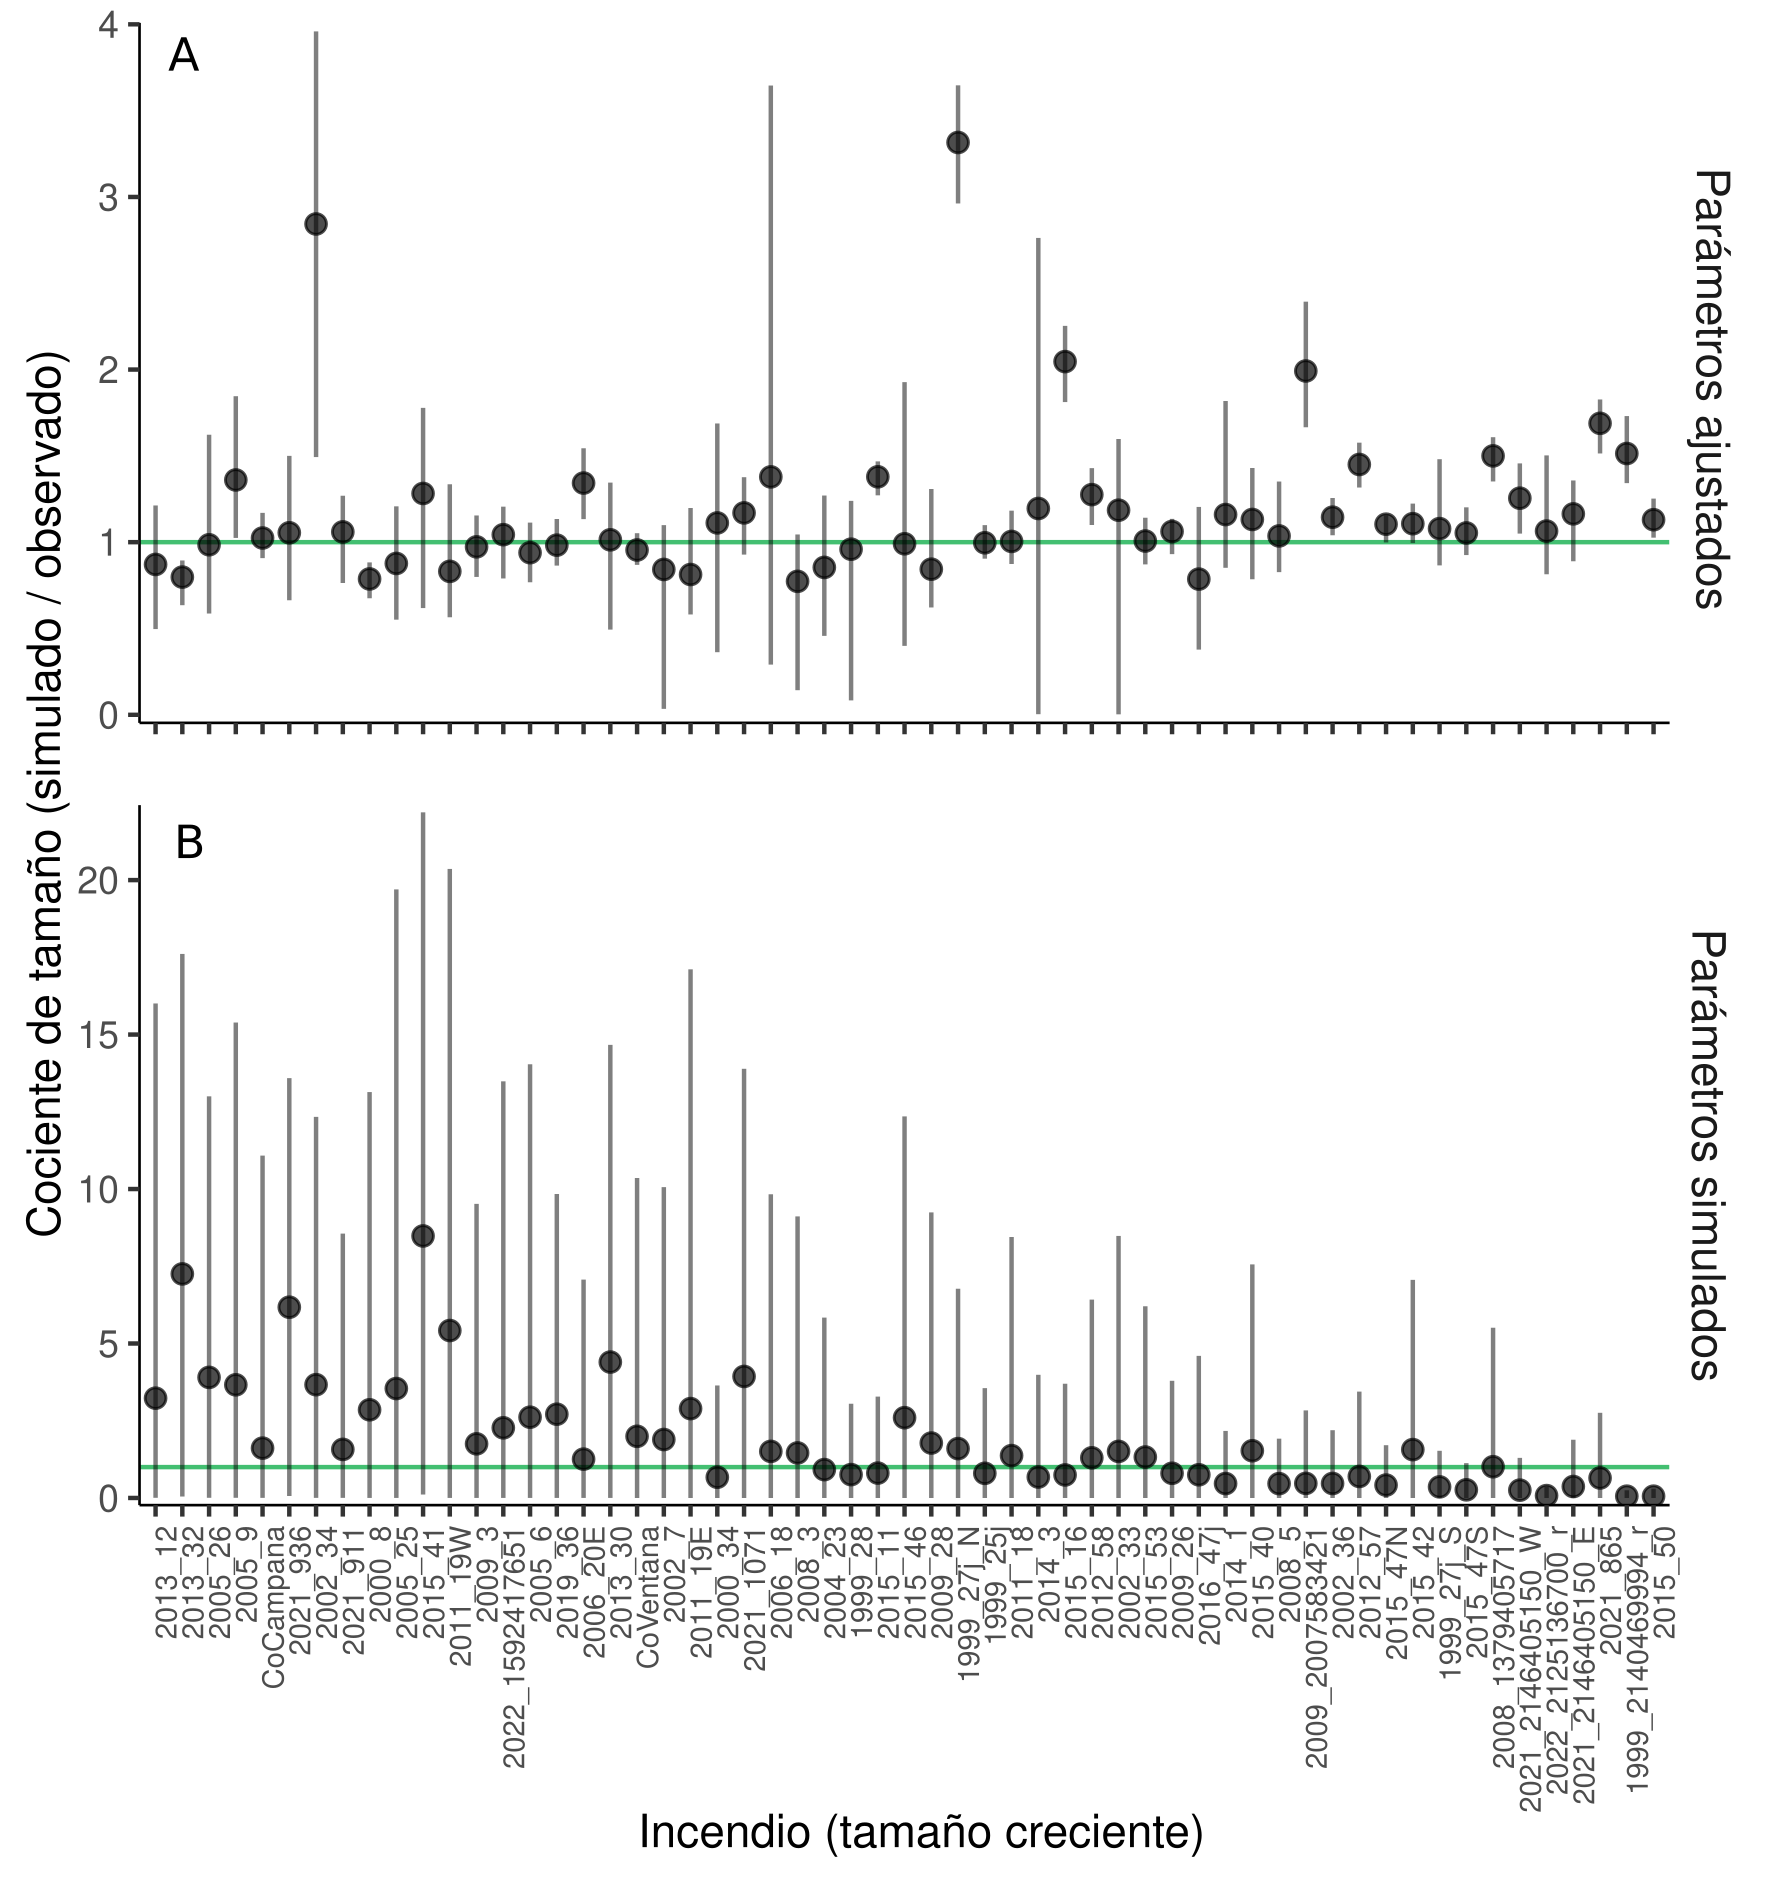
\includegraphics[width=15cm]{figuras/cap4/spread/quotient_sim_obs_fire_size.png}
  \caption[Cociente de tamaño de incendios simulados y observados.]{Cociente de tamaño de incendios simulados / observados, utilizando los parámetros ajustados para cada incendio o simulando nuevos parámetros a partir de la distribución estimada. Los puntos y líneas indican la media y el intervalo de credibilidad del 95 \% de la distribución posterior del cociente, aproximada mediante 2000 simulaciones para cada tipo de uso de los parámetros.}
  \label{fig:spread-q}
\end{figure}

\FloatBarrier

Si bien el modelo presenta un mal ajuste al usar parámetros simulados, nuestro objetivo no era desarrollar un simulador que pudiera predecir con precisión el avance del fuego en un incendio puntual, sino un simulador capaz de generar incendios similares a los que ocurren en nuestra área de estudio. Así, el mal ajuste observado al usar parámetros simulados no invalida al modelo. De hecho, a pesar de haber estimado el modelo con limitada o nula información atmosférica y de combate del fuego, se observa que el tamaño de los incendios simulados (usando parámetros simulados) es razonablemente similar a los tamaños de fuego observados (Fig.~\ref{fig:spread-q}B). 


% % Paper de respaldo 
% \newpage
% \thispagestyle{empty} % Página vacía sin encabezado ni pie
% \begin{center}
%     \vspace*{\fill} % Centrado vertical
%     {\huge \textbf{Artículo de respaldo}} % Texto grande y en negrita
%     \vspace*{\fill} % Centrado vertical
% \end{center}
% \addcontentsline{toc}{chapter}{Artículo de respaldo} % Agrega "Apéndices" al índice
% \clearpage
% \includepdf[pages=-]{secciones/10_paper_palitos.pdf} % Inserta todas las páginas del PDF

\end{document}